\documentclass[]{book}


\usepackage{svg}
\usepackage{changepage} % Include in the preamble
\usepackage{multicol} % 
\usepackage{enumitem} % 
\usepackage{fontspec}
\usepackage{xunicode}
\usepackage{polyglossia}
\usepackage{epigraph}
\usepackage{amsmath}
\usepackage{amssymb}
\setmainfont[Mapping=tex-text,Scale=1.0]{FreeSerif}
\setsansfont[Mapping=tex-text,Scale=1.0]{FreeSans}
\setmonofont{FreeMono}
\usepackage{booktabs}
\usepackage{xeCJK}
\usepackage{longtable}
\setCJKmainfont{BabelStone Han}
\newfontfamily\zh{BabelStoneHan.ttf}
\newfontfamily\zhpua{BabelStoneHanPUA.ttf}

\setdefaultlanguage[variant=american]{english}
% biblatex is used for bibtex rendering, style author-year
\usepackage[
    backend=bibtex,
    bibstyle=authoryear,
    giveninits=true,
    ibidtracker=strict,
    isbn=false,doi=false,url=false,
    labelnumber=true,
    loccittracker=strict,
    maxbibnames=10,
    maxcitenames=2,
    natbib=true,
    opcittracker=strict,
    sortcites=true,
    sorting=nyt,
    style=authoryear-ibid,
    alldates=terse,
    terseinits=false
   ]{biblatex}
\usepackage{graphicx}

\newcommand*{\img}[1]{%
    \raisebox{-.3\baselineskip}{%
        \includegraphics[
        height=\baselineskip,
        width=\baselineskip,
        keepaspectratio,
        ]{#1}%
    }%
}

\usepackage{csquotes}

\usepackage{gb4e}
\noautomath

%\let\gbtmp_
%\protected\def_{\ifincsname\string_\else\expandafter\gbtmp\fi}

\usepackage{hyperref}

\bibliography{asia.bib,references,extra}

\usepackage{color}
%\usepackage[top=0.7874in,bottom=0.7874in,left=0.7874in,right=0.7874in,nohead,includefoot,foot=12pt,footskip=26.148pt]{geometry}
\usepackage{array}
\usepackage{supertabular}
\usepackage{hhline}
\usepackage{hyperref}
%\usepackage{gb4e}
\usepackage{underscore}
\usepackage{adjustbox}
\usepackage{makecell}
\usepackage{multirow}
\usepackage{tikz}
\usetikzlibrary{tikzmark}


\noautomath
\hypersetup{colorlinks=true, linkcolor=blue, citecolor=blue, filecolor=blue, urlcolor=blue}

\newfontfamily\tib{Tibetan Machine Uni}
\newfontfamily\burm{Padauk}
\newfontfamily\sil{Charis SIL}
%\newcommand{\mydot}{\sil{ꞏ}}
\newfontfamily\grk{Galatia SIL}
\newfontfamily\kor{UnGungseo}
\newfontfamily\egy{[Aegyptus.otf]}
% Text styles
\newcommand\Bod[1]{\tibetan\textup{#1}}
\newcommand\Rom[1]{\sil\textit{#1}}
\newcommand\Gloss[1]{\sil\textup{#1}}
\newcommand\Trans[1]{\textup{#1}}
%\newcommand\Ref[1]{\textbf{\textup{#1}}}

\usepackage{enumitem}
\usepackage{setspace} 
\newcommand{\textunderset}[2]{\begin{tabular}[t]{@{}c@{}}#2\\[-0.3em]\scriptsize#1\end{tabular}}
\newcommand{\textoverset}[2]{\begin{tabular}[b]{@{}c@{}}\scriptsize#1\\[-0.45em]#2\end{tabular}}
\newcommand{\textoversetlarge}[2]{\begin{tabular}[b]{@{}c@{}}\scriptsize#1\\[-0.2em]#2\end{tabular}}
\newcommand{\textoversetnote}[2]{\begin{tabular}[b]{@{}c@{}}\scriptsize#1\\[-1.0em]#2\end{tabular}}


\usepackage{chngcntr}

%New Verison 
\counterwithout{paragraph}{subsubsection}
\setcounter{secnumdepth}{5} % Enable numbering for subparagraphs

% Paragraph numbering (repeat for each paragraph)
\renewcommand{\theparagraph}{\arabic{paragraph}}

% Subparagraph numbering (include paragraph number)
\renewcommand{\thesubparagraph}{\theparagraph\alph{subparagraph}}

% Ensure subparagraph numbering resets within each paragraph
\counterwithin*{subparagraph}{paragraph} 

% Define indentation and spacing for paragraphs
%\makeatletter
%\renewcommand{\paragraph}{%
%  \@startsection{paragraph}{4}{0pt}{1.5ex plus 1ex minus .2ex}{0.5ex plus .2ex}{\normalfont\normalsize\bfseries}%
%}

\makeatletter
\renewcommand{\paragraph}{%
  \@startsection{paragraph}{4}{0pt}{1.5ex plus 1ex minus .2ex}{-1em}{\normalfont\normalsize\bfseries}%
}
\renewcommand{\subparagraph}{%
  \@startsection{subparagraph}{5}{1.5em}{1ex plus .2ex}{-1em}{\normalfont\normalsize\bfseries}%
}
\makeatother





\title{Chinese: a dialectical history}
\author{Nathan W. Hill}


\begin{document}

\frontmatter
\maketitle

\tableofcontents


\mainmatter

%\chapter{諧聲 `\emph{xiéshēng} series':  phonetic information in the structure of Chinese characters}
\chaptermark{\textit{xiéshēng} series}

\epigraph{Treasure your exceptions! When there are none, the work gets so
dull that no one cares to carry it further. Keep them always uncovered and in sight. Exceptions are like the rough brickwork of a
growing building which tells that there is more to come and shows
where the next construction is to be.}{William Bateson 1908}



%\section{Structure of Chinese Characters}

\paragraph{}
The Chinese script, a fully developed writing system, abruptly emerges around 1250 BCE. 
Some Chinese characters are simple logograms---that is, symbols whose graphic shapes directly (iconically) represent the things they denote---for example 馬 \textit{maeX} `horse', being originally an image of a horse (see Figure \ref{fig:horse}). 
However the great majority of Chinese characters, throughout the writing system's history have consisted of a phonetic component and a semantic component. For instance, examining the character for `headboard', 榪 \textit{maeH}, we observe a semantic component on the left, 木 \textit{muwK} `tree', and a phonetic component on the right, 馬 \textit{maeX} `horse'
 (see Figure \ref{fig:headboard}). 
A suite of characters derived from the same phonetic component we refer to as a `\textit{xiéshēng} series'.\footnote{
Several scholars have prepared lists of \textit{xiéshēng} series; these include Zhu Junsheng 朱駿聲
(1788-1858) in his 說文通訓定聲
 \emph{Shuōwén tōngxùn dìngshēng} (1832), \citet[]{Karlgren1957}, and \citet[]{Schuessler2009minimal}. There has been little explicit discussion of the principles for compiling such lists. Many choces are obvious and controversies generally are restricted to whether or not, on the basis of paleographic relationships no longer visible in the current form of the characters, to unite together series that earlier scholars have kept apart. Thus, 
\citet[143]{Baxter2014OldChinese}
put 喪  \emph{saṅ} `obsequeis'
%(03-54a) 
in the series built on 亡~ \emph{miaṅ} `perish', 
%(03-65a), 
but 
\citet[87]{Schuessler2009minimal}
demurs.} Because at the time that any given character was coined, the pronunciation of the word that the character in question wrote must have been quite similar to the character that serves as its phonetic components, such \textit{xiéshēng} series provide a window onto the pronunciation of ancient times. Nonetheless, we must recognize that when looking at Old Chinese morphemes in the garb of Middle Chinese phonology, the difference between the Middle Chinese pronunciations of two morphemes that are written with characters making use of the self-same phonetic component may be credited either to (1) differences in their pronunciation that were already present when the characters in question were coined (but which were deemed sufficiently small to not stand in the way of using the same phonetic in both morphemes) or to (2) differences in their pronunciation that have arisen over time. Distinguishing these two is a methodological hornets nest. Luckily, however, because of the
\textit{Ausnahmslosigkeit der Lautgesetze} differences of the second type generally arise as differences of the first type. As such, differences in Middle Chinese pronunciation can qua differences in any event,  be back-projected onto Old Chinese
at least in the first instance.\footnote{The caveat `in the first instance' is necessary because of borrowings, analogical developments, onomatopaeia, and the like.}
 The phonetic nature of these differences may safely be assumed to have changed between Old Chinese and Middle Chinese, but the phonetic nature of a given difference in the early period and in the later period will naturally have a non-fortuitous relationship. 

\begin{figure}[tbp]
    \centering

    % First figure (Oracle Bone Character)
    \begin{parbox}{0.45\textwidth} % Adjust width as needed
        \centering
        
\includegraphics[width=0.1\textwidth]{Chapter2/OBIhorse.png}
        \caption{The Oracle bone character for `horse'}
        \label{fig:horse}
        \end{parbox}

     \vspace{10mm}

    % Second figure (Table)
    \begin{parbox}{0.45\textwidth} % Adjust width as needed
        \centering
\begin{tabular}{r l c r l c l}
  \Huge{木} & \large{`tree'} & {\raisebox{2ex}{+}} &
  \Huge{馬} & {\raisebox{3ex}{\large{\textit{maeX}}}} & {\raisebox{2ex}{=}} & 
  %
  % ---- A subtable in the last column ----
   \begin{tabular}[b]{@{}l@{\hspace{0.8em}}l@{}}
    % Column 1 of subtable: the big character
    \Huge{榪} 
    &
    % Column 2 of subtable: stacked text
    \begin{tabular}[b]{@{}l@{}}
      \large{\textit{maeH}}\\
      \large{`headboard'}
    \end{tabular}
  \end{tabular}
  \\
\end{tabular}

        
        \caption{Semantic and phonetic components of 榪 `headboard'}
        \label{fig:headboard}
 
    \end{parbox}

\end{figure}


In order to bring the discussion down to a more concrete level, I allow myself a sneak peak at things to come. The character 凋 \emph{tew} `wither'  contains as its phonetic the character 周 \emph{ciuw} `circle, whole'. A look at the Middle Chinese initial of the two morphemes, viz. \textit{t-}
and \textit{c-} (IPA [{\sil{tʃ-}}]), will immediately lead one to wonder whether in Old Chinese the morpheme written with 周 did not also begin with *t-, since the change of *t- to \textit{c-} is one of the most common and straightforward sound changes known in the world's languages. This proposal classifies the difference between  \textit{t-}
and \textit{c-} as belonging to type (2)---a difference in their pronunciation that arose over time, but at the cost of implicitly proposing that the condition for palatalization was a difference belonging to type (1)---a difference already present in the pronunciation of the two morphemes in Old Chinese, but a sufficiently small one to have not stood in the way of them employing the same phonetic. We can only pay Peter for differences in Middle Chinese with the wherewithal provided by Paul in the form of differences already present in Old Chinese. 
There is a way, however, to keep our debts to Paul from spiraling out of control; if we could credit an ignorable phonetic difference in Old Chinese as the conditioning environment for many irksome phenomena confronted in \textit{xiéshēng} in Middle Chinese garb, this would let us offer to Paul for strikingly large phonetic differences in Middle Chinese again and again the same well worn Old Chinese penny. 
In the case of 凋 \emph{tew} `wither'  and 周 \emph{ciuw} `circle, whole', for example, 
we can propose that the phonetic origin of what the -\textit{i}- in Middle Chinese indexes, is also what triggered the change of *t-to \textit{c}-. 
To further wear this metaphor out, paying ``debts'' of Middle Chinese phonetic differences with Old Chinese ``funds'' is in essence how \textit{xiéshēng} series are used in the reconstruction of Old Chinese. Before lunging headlong into an exploration of the various phenomena that occur in \textit{xiéshēng} series, we must arm ourselves with an overall impression of how close the pronunciation of two morphemes must have been in order to be written with characters that share a phonetic. To form this impression we start with a very simple \textit{xiéshēng} series (§\ref{par:simplest-XS-series}) and then modify our initial impressions with recourse to a still simple, but not quite as simple series (§\ref{par:still-simple-XS-series}).

\paragraph{The simplest type of \textit{xiéshēng} series.}
\label{par:simplest-XS-series}
Let us look at a few \textit{xiéshēng} series to explore parameters of phonetic difference that are found in their Middle Chinese readings. Focusing still on the \textit{xiéshēng} series built on 馬 \textit{maeX} `horse', we encounter variations such as:

\begin{itemize}
\item {\Large{馬}} \textit{maeX} `horse'
\item {\Large{榪}} \textit{maeH} `headboard'
\item {\Large{禡}} \textit{maeH} `war sacrifice'
\item {\Large{罵}} \textit{maeH}, \textit{maeX} `scold'
\end{itemize}

\noindent In this case, all of the readings share an initial 明 \textit{m-} and a rime -\textit{ae-} (O-II-麻-\textsc{cannabis}-smooth), and they vary only in tone (-\textit{H} for 去聲 \textit{qùshēng} and -\textit{X} for 上聲 \textit{shǎngshēng}).
Our options are to conclude (1) that tone was ignorable when coining new characters or (2) that the tones arose from some yet more ignorable phonetic difference. But setting tone aside as we clearly should, shall we hypothesize that two morphemes must share an initial and a rime in Old Chinese to employ the same phonetic? 

In service of the goal of symbolically representing the phonetic information indicated by the presence of the character 馬 \textit{maeX} as the phonetic component of another character, we can at this point write \textbf{mae}.  This transcription indicates that all morphemes written with this phonetic share initial \textbf{m-} and they also share the vowel \textbf{-ae-}. This notation also indicates that no information is furnished by the phonetic about the tone of the morphemes by how they are written. As proposed in \cite{hill_proposal_2015}, the semantic components may be written with abbreviated Latin words set in superscript. Thus, provisionally : 

\begin{itemize}
\item {\Large{馬}} \textbf{{\large{mae}}}, \textit{maeX} `horse'
\item {\Large{榪}} {\large{{\textsuperscript{arb}}mae}}, \textit{maeH} `headboard'
\item {\Large{禡}} {\large{{\textsuperscript{spirit}}mae}}, \textit{maeH} `war sacrifice'
\item {\Large{罵}} {\large{{\textsuperscript{nas}}mae}}, \textit{maeH}, \textit{maeX} `scold'
\end{itemize}

This approach to transcription captures the essential phonetic uniformity across the series by abstracting away from tonal variation and concentrating on the common initial and rime. 

\paragraph{A still quite simple \textit{xiéshēng} series.}
\label{par:still-simple-XS-series}
To test our ability to generalize what we have learned in our examination of the series built on 馬 \textit{maeX} `horse', we look next at a somewhat more complicated series. 

\begin{itemize}
    \item {\Large{皮}} \textit{bie} `skin'
    \item {\Large{被}} \textit{bieX} `cover'
    \item {\Large{陂}} \textit{pie} `pond'
    \item {\Large{披}} \textit{phie} `drape'
    \item {\Large{跛}} \textit{paX} `lame'
    \item {\Large{破}} \textit{phaH} `defeat'
\end{itemize}

This series showcases three initials, viz. 幫 \textit{p}-, 滂 \textit{ph}-, 並
\textit{b}-, and two rimes, viz. the Middle Chinese %type A 
rime -\textit{a} (O-I-歌-\textsc{carmen}-smooth) and the Middle Chinese 
%type B 
rime -\textit{ie} (O-III-支-\textsc{ramus}-smooth). After examining the \textit{xiéshēng} series built on 馬 \textit{maeX} `horse', we had  hypothesized that two morphemes must share an initial and a rime in Old Chinese to employ the same phonetic. This series built on 皮 \textit{bie} has negated this hypothesis, which now stands in need of revision. 

The series build on 皮 \textit{bie} `skin' exhibits the initials 
幫 \textit{p}-, 滂 \textit{ph}-, and 並
\textit{b}- but it does not exhibit 明 \textit{m}- (the initial seen in the series build on 馬 \textit{maeX} `horse'). The evidence of these two series taken together may thus be subsumed into the new hypothesis that for two morphemes to be written with the same phonetic they must have homorganic initials, either all stops or all nasals, and that they must either all have the same rime, or all have one of two rimes.  

\paragraph{The A/B-phenomenon.}
\label{par:A/B-phenomenon}
In the transcription of Middle Chinese that I am here using the orthographic medial -\textit{i-} indexes some phenomena in Middle Chinese that need not concern us here, instead we can note that this medial -\textit{i-} redundantly encodes one of the two rimes found in the series. As a point of terminology we call the Old Chinese ancestors of those syllables containing this Middle Chinese -\textit{i-} `type B syllables' and the Old Chinese ancestors of those Middle Chinese syllables lacking this -\textit{i-} we in contrast call `type A sylables'. 

The \textit{xiéshēng} series built on 皮 \textit{bie} `skin', thus exhibits the type A rime -\textit{a} 
 (O-I-歌-\textsc{carmen}-smooth) 
and the type B rime -\textit{ie} (O-III-支-\textsc{ramus}-smooth). We will hereafter refer to such a pair of rimes, one rime from type A and one from type B, as a  `\textit{xiéshēng} rhyme pair.'\footnote{More formally, we define a `\textit{xiéshēng} rhyme pair' \{v, w\}, where -\textit{v} and -\textit{w} are rimes appearing in a \textit{xiéshēng} series, only and exactly one of which has a medial -\textit{i-} in its Middle Chinese reading. We can now define a relationship `is member of a \textit{xiéshēng} rhyme pair'. Now, if x is a member of a \textit{xiéshēng} rhyme pair X, then X contains x as one of its two members, in other words `being in the \textit{xiéshēng} rhyme pair X' is reflexive. If x is a member of the same \textit{xiéshēng} rhyme pair as y, then y is a member of the same  \textit{xiéshēng} rhyme pair as x, so the relationship is symetrical. If x, is in the same pair with y, and y is in the same pair with z, then x = z, and indeed z and y are in the same pair, so the relationship is also transitive. Thus, being a member of a \textit{xiéshēng} rhyme pair creates an equivalence relation, which allows us to identify the pair as `the same rime' if we choose to do so. The relationship is analogous to an electron and a proton being part of the same hydrogen atom, where it is a question of focus whether refer to `this hydrogen atom' as a particle or `this proton' as a particle.

This definition of a \textit{xiéshēng} rime pair only fully works if there are exactly two rimes, one type A and one type B, in a particular series. Such series exist, for example those built on  虍 \textit{hu} `tiger',   巨 \textit{giəX}, \textit{kiuX} `huge', and 襄 \textit{siaṅ} `support'. However, there are also many series that contain only one rime, for example those built on 吳 \textit{ṅu} `the state of Wu',  宁 \textit{ḍiə}, \textit{ḍiəX} `reserve', 舁 \textit{yiəX} `carry on one's shoulder', etc., and there are also many series that contain more than two rimes, for example those built on 号 \textit{ḫawH} `number',  夭 \textit{'awX} `young' (n.), \textit{'iewX} `die prematurely', etc. Methodologically, we can treat the single rhyme series as equivalent to the relevant pair that contains this particular rime as a member. I do this, for example, for the series built on 剌 \textit{lat}  `contrary' (see sec. \ref{sec:xiesheng-l-t}, §\ref{par:at-iet-XS-pair}).
However, for series with more than two rimes, what we will do is simply narrow our focus in the first instance to a pair of rimes, particularly one that is a tested in other series as the only rimes of that series, and we will widen our focus explicitly later.} 
At this juncture \textit{ex hypothesi} a single series will at maximum exhibit a pair of rimes, one of them type A and one of them type B, so as a provisional matter of pure convention for the purpose of transliterating the phonetic information contained in the series as such, we may index the pair of rimes with the type A member.\footnote{In fact some \textit{xiéshēng} series exhibit only type B rimes or exhibit more than one type A rime, and in such cases I allow myself to use the prevailing type B rime in the transliteration of the series as a whole.} 
In like fashion, in the transliteration of the phonetic information encoded by membership in the series, we may use \textbf{p-} as a cover symbol for 
幫 \textit{p}-, 滂 \textit{ph}-, and 並
\textit{b}-. 
Thus, provisionally:

\begin{itemize}
    \item {\Large{皮}} {\large{\textbf{pa}}}, \textit{bie} `skin'
    \item {\Large{被}} {\large{\textsuperscript{vest}pa}}, 
\textit{bieX} `cover'
    \item {\Large{陂}} {\large{\textsuperscript{tum}pa}}, \textit{pie} `pond'
    \item {\Large{披}} {\large{\textsuperscript{man}pa}}, 
\textit{phie} `drape'
    \item {\Large{跛}} {\large{\textsuperscript{ped}pa}}, \textit{paX} `lame'
    \item {\Large{破}} {\large{\textsuperscript{lap}pa}}, 
\textit{phaH} `defeat'
\end{itemize}


The disadvantage of this choice of notation is that, if we use -\textbf{a} to index the pair of type A -\textit{a} and type B -\textit{ie}, then our writing 馬 \textbf{mae} above now appears to index a pair of rimes of which -\textit{ae} is the type A member, whereas in fact this series only has he one rime -\textit{ae} in it. Because series that mix a type A and a type B rime are more prevalent than those that exhibit only one rime, it is notationally more convenient to mark the rarer unmixed series. The series built on 馬 \textit{maeX} we accordingly revise as follows: 

\begin{spacing}{0.75} 
\begin{itemize}[noitemsep]
\item {\Large{馬}} \textbf{{\large{m\textoverset{a}{a}e}}}, \textit{maeX} `horse'
\item {\Large{榪}} {\large{{\textsuperscript{arb}}m\textoverset{a}{a}e}}, \textit{maeH} `rafter'
\item {\Large{禡}} {\large{{\textsuperscript{spirit}}m\textoverset{a}{a}e}}, \textit{maeH} `war sacrifice'
\item {\Large{罵}} {\large{{\textsuperscript{nas}}m\textoverset{a}{a}e}}, \textit{maeH}, \textit{maeX} `scold'
\end{itemize}
\end{spacing}

The structure of the Chinese script often acknowledges both the phonetic commonality of the two component rimes of a \textit{xiéshēng} rime pair and the phonetic distinctiveness of its two component rimes. 
Witness the following series: 

%\begin{itemize}
%    \item {\large{我}}  
%    {\large{\textbf{ṅa}}}, 
%    \textit{ṅaX} `we'
%    \item {\Large{俄}} 
%    {\large{{\textsuperscript{hom}}ṅa}}, 
%    \textit{ṅa} `sudden'
%    \item {\Large{娥}} 
%    {\large{{\textsuperscript{fem}}ṅa}},
%    \textit{ṅa} `beautiful'
%    \item {\Large{峨}} 
%    {\large{{\textsuperscript{mon}}ṅa}},
%    \textit{ṅa} `lofty'
 %   \item {\Large{睋}} 
 %   {\large{{\textsuperscript{ocul}}ṅa}},
 %   \textit{ṅa} `gaze'
 %   \item {\Large{莪}} 
  %  {\large{{\textsuperscript{herb}}ṅa}},
  %  \textit{ṅa} `zedoary'
  %  \item {\Large{蛾}} 
  %  {\large{{\textsuperscript{serp}}ṅa}},
  %  \textit{ṅa} `moth',
  %  \textit{ṅieX} `ant'
  %  \vspace{-2mm}
%    \begin{spacing}{0.8} 
%        \item 
%        {\Large{義}} 
        %{\large{{\textsuperscript{ov:}}ṅa}} =
        %{\large{\textbf{ṅ\textoverset{b}{a}}}},
       % \textit{ṅieH} `righteousness'
   % \end{spacing}
   % \vspace{-2mm}
   % \begin{itemize}[noitemsep]
   % \begin{spacing}{0.8} 
    %    \item {\Large{儀}} 
        %{\large{{\textsuperscript{hom}}ṅ\textoverset{b}{a}}},
   %     \textit{ṅie} `ceremony'
    %    \item {\Large{議}} 
        %{\large{{\textsuperscript{dic}}ṅ\textoverset{b}{a}}},
     %   \textit{ṅieH} `discussion'
        \item %{\Large{蟻}} 
        %{\large{{\textsuperscript{serp}}ṅ\textoverset{b}{a}}},
      %  \textit{ṅieX} `ant'
   % \end{spacing}
    %\end{itemize}
%\end{itemize}

%\noindent The subseries built on 義  \textit{ṅieH} `righteousness' consists entirely of type B readings with the rime 
%-\textit{ie} (O-III-支-\textsc{ramus}-smooth).\footnote{The series built on 我 \textit{ṅaX} itself, were it not for the one reading \textit{ṅieX} for 蛾 `ant' (and naturally for 義  \textit{ṅieH} considered as a child of  
%我 \textit{ṅaX}) `we', would consist entirely of type A readings with the rime -\textit{a} (O-I-歌-\textsc{carmen}-smooth).} 

\begin{itemize}
    \item {\Large{\symbol{135740}}} % 广 + 丁
    {\large{teṅ}}, \textit{theṅX}
    `court`
    \begin{spacing}{0.85} 
    % 09-17/0835d
    \item {\Large{廷}} % 廴 + 壬/延 
    {\large{{\textsuperscript{progred}}teṅ}} =
        {\large{\textbf{t\textoverset{a}{e}ṅ}}},
    \textit{deṅ, deṅH}
    `court`
\end{spacing}

\vspace{-1mm}

\begin{itemize}
    \begin{spacing}{0.85} 
    % 09-17/0835h
    \item {\Large{庭}} % 广 + 廷
    {\large{{\textsuperscript{lax}}t\textoverset{a}{e}ṅ}},
    \textit{deṅ, theṅH}
    `court`

    % 09-17/0835i
    \item {\Large{挺}} % 扌 + 廷
    {\large{{\textsuperscript{man}}t\textoverset{a}{e}ṅ}},
    \textit{deṅX, theṅX}
    `draw` (a weapon)

    % 09-17/0835m
    \item {\Large{霆}} % 雨 + 廷
    {\large{{\textsuperscript{pluv}}t\textoverset{a}{e}ṅ}}, \textit{deṅ}
    `thunder`
    \end{spacing}
\vspace{-1mm}
   
\end{itemize}
\vspace{-1mm}
    % 09-17/0835r
    \begin{spacing}{0.8} 
    \item %{\Large{呈}} 
    
\includegraphics[width=1.4em]{Chapter2/呈.png}
    {\large{{\textsuperscript{or}}teṅ}} = {\large{\textbf{ḍ\textoverset{b}{e}ṅ}}}, \textit{ḍieṅ}
    `submit`
\end{spacing}
    \vspace{-1mm}

\begin{itemize}
    \begin{spacing}{0.8} 
     % 09-17/0835s
    \item {\Large{珵}} % 王 + 廷
    {\large{{\textsuperscript{gem}}ḍ\textoverset{b}{e}ṅ}},
    \textit{ḍieṅ} `jade pendant`

    % 09-17/0835t
    \item {\Large{程}} % 禾 + 呈
    {\large{{\textsuperscript{gran}}ḍ\textoverset{b}{e}ṅ}}, \textit{ḍieṅ}
    `measure` (n.)

    % 09-17/0835u
    \item {\Large{裎}} % 衣 + 呈
    {\large{{\textsuperscript{vest}}ḍ\textoverset{b}{e}ṅ}}, \textit{ḍieṅ}
    `be naked`
    \end{spacing}
\end{itemize}
\end{itemize}

\noindent The subseries built on 廷   \textit{deṅ, theṅH} `court' consists entirely of type A readings with the rime 
-\textit{eṅ} (O-IV-青-\textsc{vireo}-smooth) and the subseries built on 呈 \textit{ḍieṅ}
    `submit`
     consists entirely of type A readings with the rime 
-\textit{ieṅ} (O-A-清-\textsc{purus}-smooth) . 

\paragraph{Degrees of phonetic precision in \textit{xiéshēng} series.}
\label{par:precision-in-xiesheng}
The example of the series built on 
\symbol{135740} \textit{teṅ, theṅX} `court'
%我     \textit{ṅa} `we' 
and its subseries built on 
廷 \textit{deṅ, deṅH} `court'
and 
呈 \textit{ḍieṅ} `submit`
%義 \textit{ṅieH} `righteousness' 
makes the more general point that in principle a \textit{xiéshēng} series can be more or less precise in terms of the phonetic information that it imparts, and our transcription system is flexible enough to accommodate these varying degrees of precision. There are indeed series, such as the following, that clearly indicate tone, in this case -\textit{H} (去聲 \textit{qùshēng}).

\begin{itemize}
    \item {\Large{㒸}}  % 29-09/0526a  
    {\large{\textbf{zwiyH}}},  
    \textit{zwiyH}       % 0526a  
    `follow'

    \item {\Large{隊}}  % 29-09/0526f  
    {\large{\textsuperscript{tum}zwiyH}},  
    \textit{ḍwiyH, dwəyH}       % 0526f  
    `troop'
\begin{itemize}
    \item {\Large{墜}}  % 29-09/0526g  
    {\large{\textsuperscript{terr}zwiyH}},  
    \textit{ḍwiyH}       % 0526g  
    `plummet'
\end{itemize}

    \item {\Large{遂}}  % 29-09/0526d  
    {\large{\textsuperscript{eo}zwiyH}},  
    \textit{zwiyH}       % 0526d  
    `follow'
\begin{itemize}
    \item {\Large{檖}}  % 29-09/0526h  
    {\large{\textsuperscript{arb}zwiyH}},  
    \textit{zwiyH}       % 0526h  
    `Chinese wild pear'

    \item {\Large{燧}}  % 29-09/0526i  
    {\large{\textsuperscript{ign}zwiyH}},  
    \textit{zwiyH}       % 0526i  
    `flint'

    \item {\Large{璲}}  % 29-09/0526j  
    {\large{\textsuperscript{gem}zwiyH}},  
    \textit{zwiyH}       % 0526j  
    `pendant girdle ornament'

    \item {\Large{穟}}  % 29-09/0526k  
    {\large{\textsuperscript{gran}zwiyH}},  
    \textit{zwiyH}       % 0526k  
    `ear' (of grain)

    \item {\Large{襚}}  % 29-09/0526l  
    {\large{\textsuperscript{vest}zwiyH}},  
    \textit{zwiyH}       % 0526l  
    `shroud'

    \item {\Large{隧}}  % 29-09/0526m  
    {\large{\textsuperscript{tum}zwiyH}},  
    \textit{zwiyH}       % 0526m  
    `tunnel'

    \item {\Large{旞}}  % 29-09/0526n  
    {\large{\textsuperscript{vex}zwiyH}},  
    \textit{zwiyH}       % 0526n  
    `aigrette of a carroccio'

    \item {\Large{邃}}  % 29-09/0526o  
    {\large{\textsuperscript{cav}zwiyH}},  
    \textit{swiyH}       % 0526o  
    `profound'
\end{itemize}
\end{itemize}
%3
 %   29-09/0526a 㒸 zwiyH
 %   29-09/0526d 遂 zwiyH
 %   29-09/0526f 隊 ḍwiyH, dwəyH
 %   29-09/0526g 墜 ḍwiyH
 %   29-09/0526h 檖 zwiyH
 %   29-09/0526i 燧 zwiyH
 %   29-09/0526j 璲 zwiyH
 %   29-09/0526k 穟 zwiyH
 %   29-09/0526l 襚 zwiyH
 %   29-09/0526m 隧 zwiyH
 %   29-09/0526n 旞 zwiyH
 %   29-09/0526o 邃 swiyH

There are also series that uniformly have -\textit{X} (上聲 \textit{shǎngshēng}), but such series tend to be short. Here is one example: 



\begin{itemize}
    \item {\Large{禹}}  % 01-25/0099a  
    {\large{\textbf{ḫiuX}}},  
    \textit{hiuX}       % 0099a  
    `Yu the Great, legendary flood hero'

    \item {\Large{偊}}  % 01-25/0099d  
    {\large{\textsuperscript{hom}ḫiuX}},  
    \textit{ḫiuX}       % 0099d  
    `step by step' (in 偊偊)  

   % \item {\Large{楀}}  % 01-25/0099e  
   % {\large{\textsuperscript{arb}ḫiuX}},  
   % \textit{kiuX}       % 0099e  
   % `a kind of tree' (?)

    \item {\Large{萭}}  % 01-25/0099f  
    {\large{\textsuperscript{herb}ḫiuX}},  
    \textit{kiuX}       % 0099f  
    `wheelwright's truing reed'

    \item {\Large{踽}}  % 01-25/0099g  
    {\large{\textsuperscript{ped}ḫiuX}},  
    \textit{kiuX}       % 0099g  
    `step by step' (in 踽踽)
\end{itemize}

%5
%    26-23/0597a 豊 lejX
%    26-23/0597d 禮 lejX
%    26-23/0597e 醴 lejX
%    26-23/0597h 鱧 lejX
%    26-23/0597i 體 thejX



%5
%    07-28/0871a 徙 sjeX
%    07-28/0871b �� sjeX
%    07-28/0871f 蓰 sjeX
%    07-28/0871g 屣 srjeX
%    07-28/0871h 縰 srjeX


%4
%    04-32/0967a 巳 ziX
%    04-32/0967d 祀 ziX
%    04-32/0967i 汜 ziX
%    04-32/0967k 戺 dzriX


%4
%    09-05/0810a 幸 heangX
%    09-05/0810b 倖 heangX
%    09-05/0810c 婞 hengX
%    09-05/0810d 涬 hengX

%4
%    26-04/0588a 启 khejX
%    26-04/0588c 啟 khejX
%    26-04/0588h 綮 khejX
%    26-04/0588j 晵 khejX


%4
%    27-17/0583a 尾 mjɨjX
%    27-17/0583c 娓 mjɨjX
%    27-17/0583d 浘 mjɨjX
%    27-17/0583e �� xjwɨjX

%    26-28/0554b 姊 tsijX
%    26-28/0554c 姉 tsijX
%    26-28/0554d 秭 tsijX
%    26-28/0554f 笫 tsrijX
%    26-28/0554g 胏 tsrijX
%    26-28/0554h 柹 dzrijX
%    26-28/0554i 柿 dzrijX
%    26-28/0554j 䪡 tsej



%    10-34/1229a 奏 tsuwH
%    10-34/1229b 湊 tshuwH
%    10-34/1229c 腠 tshuwH

 %   21-16/0336a 筮 dzyeyH
  %  21-16/0336b 簭 dzyeyH
  %  21-16/0336c 噬 dzyeyH
  %  21-16/0336d 澨 dzyeyH

   % 24-05/0143a 寒 han
   % 24-05/0143d 搴 kjenX
   % 24-05/0143e 謇 kjenX
   % 24-05/0143f 蹇 kjenX, kjonX
  %  24-05/0143g 褰 khjen
  %  24-05/0143h 騫 kjonX
   % 24-05/0143i 攓 kjenX, kjonX

  %  24-48/0182a 般 ban, pan
  %  24-48/0182d 槃 ban
  %  24-48/0182e 盤 ban
  %  24-48/0182g 磐 ban
  %  24-48/0182h 縏 ban
  %  24-48/0182i 鞶 ban

  %  34-15/0461a 熏 xjun
  %  34-15/0461d 燻 xjun
  %  34-15/0461e 薰 xjun
  %  34-15/0461f 勳 xjun
  %  34-15/0461g 獯 xjun
  %  34-15/0461h 纁 xjun
   % 34-15/0461i 臐 xjun
   % 34-15/0461j 壎 xjwon

%7
    %29-08/0533a 惠 hweyH
    %29-08/0533b 叀 hweyH
    %29-08/0533e 蟪 hweyH
    %29-08/0533f 蕙 hweyH
    %29-08/0533g 譓 hweyH
    %29-08/0533h 穗 zwiyH
    %29-08/0533i 繐 sjweyH

%29-09

%13
 %   29-09/0526a 㒸 zwiyH
 %   29-09/0526d 遂 zwiyH
 %   29-09/0526f 隊 drwiyH, dwoyH
 %   29-09/0526g 墜 drwiyH
 %   29-09/0526h 檖 zwiyH
 %   29-09/0526i 燧 zwiyH
 %   29-09/0526j 璲 zwiyH
 %   29-09/0526k 穟 zwiyH
 %   29-09/0526l 襚 zwiyH
 %   29-09/0526m 隧 zwiyH
 %   29-09/0526n 旞 zwiyH
 %   29-09/0526o 邃 swiyH

%29-10

  %  29-10/0527a 彗 zjweyH, zwiyH
  %  29-10/0527b 篲 zjweyH, zwiyH
  %  29-10/0527c 嘒 xweyH
  %  29-10/0527d 慧 hweyH
  %  29-10/0527e 譿 hweyH

 %   29-34/0518a 四 siyH
  %  29-34/0518e 駟 siyH
   % 29-34/0518f 柶 siyH
    %29-34/0518g 泗 siyH

%10
 %   30-02/0515a 旡 kjɨyH
  %  30-02/0515c 既 kjɨyH
   % 30-02/0515g 蔇 giyH, kjɨyH
    %30-02/0515h 塈 giyH, xiyH, xjɨyH
%    30-02/0515i 摡 koyH, xjɨyH
%    30-02/0515j 㮣 koyH
%    30-02/0515k 概 koyH
%    30-02/0515l 溉 koyH
%    30-02/0515m 嘅 khoyH
%    30-02/0515n 慨 khoyH
%    30-02/0515o 暨 giyH

 %   30-11/0509a 隶 doyH, yiyH
 %   30-11/0509c 逮 deyH, doyH
 %   30-11/0509e 曃 thoyH
 %   30-11/0509f 棣 deyH
 %   30-11/0509g 肄 yiyH
 %   30-11/0509h 肆 siyH
 %   30-11/0509m 㣈 siyH
 %   30-11/0509n 蕼 siyH
 %   30-11/0509o 肂 siyH, yiyH
 %   30-11/0509p 殔 siyH, yiyH
 %   30-11/1241m 隸 leyH


%    31-05/0523a 胃 hjwɨyH
%    31-05/0523c 媦 hjwɨyH
%    31-05/0523d 謂 hjwɨyH
%    31-05/0523f 蝟 hjwɨyH
%    31-05/0523g 喟 khweayH, khwiyH

 %   32-24/0469a 舜 sywinH
 %   32-24/0469b 蕣 sywinH
 %   32-24/0469c 瞬 sywinH
 %   32-24/0469d 瞚 sywinH

 %   32-35/0363a 卂 sinH
 %   32-35/0363b 迅 swinH
 %   32-35/0363c 訊 sinH
 %   32-35/0363d 䒖 sinH

 %   24-56/0266a 曼 manH, mjonH
 %   24-56/0266d 蔓 mjonH
 %   24-56/0266e 嫚 maenH
 %   24-56/0266g 僈 maenH
 %   24-56/0266h 慢 maenH, manH
 %   24-56/0266i 墁 man
 %   24-56/0266j 幔 manH
 %   24-56/0266k 縵 manH
 %   24-56/0266l 鄤 manH
 %   24-56/0266n 漫 maenH, manH
 %   24-56/0266o 謾 maenH, man, manH, mjen

 %   31-02/0540a 㬰 gwiyH
 %   31-02/0540b 貴 kjwɨyH
 %   31-02/0540c 憒 kwoyH
 %   31-02/0540d 潰 hwoyH
 %   31-02/0540e 繢 hwoyH
 %   31-02/0540f 靧 xwoyH
 %   31-02/0540g 匱 gwiyH
  %  31-02/0540h 櫃 gwiyH
  %  31-02/0540i 蕢 gwiyH
  %  31-02/0540j 簣 khweayH
  %  31-02/0540k 鞼 gwiyH
  %  31-02/0540l 饋 gwiyH
  %  31-02/0540m 遺 ywij, ywiyH
  %  31-02/0540o 僓 xweayH
  %  31-02/0540p 聵 ngweayH
  %  31-02/0540q 壝 ywij, ywijX




%\section{The \textit{xiéshēng} dogma}
\paragraph{} We have come far enough to articulate the `\textit{xiéshēng} dogma' that will guide our exploration of Old Chinese from here on out. This dogma may now read ``the Old Chinese readings of characters with the same phonetic component share the same rime and a homorganic initial, without mixing stops and resonants''.\footnote{Duan Yucai 段玉裁 (1735-1815) proposed that characters sharing the same phonetic component would have rhymed in the language of the \textit{Shījīng}. Li Fang-Kuei 
\citeyearpar[228]{Li1974} further stipulated that they should have homorganic initials. 
See also \citet[348]{Baxter1992} and \citet[11]{schuessler_minimal_2009}.}
If we come up with a series of sound changes that, if undone reverse chronologically, took us from middle Chinese to a form of Old Chinese that adhered to this dogma, we would have won at the game of Old Chinese reconstruction. 

Once again allowing ourselves to sneak a peak into our own future results, the \emph{xiéshēng} series built on 皮  \emph{bie} %(18-16) 
illustrates
both the rime and the initial facets of the \emph{xiéshēng} hypothesis, in the reconstruction of Baxter and Sagart.

\begin{itemize}
\item {\Large{皮}} \textit{bie} < *{\sil{m-p(r)aj}} `skin`
\item {\Large{被}} 
\textit{bieX} < *{\sil{m-pʰ(r)ajʔ}} `cover`
%\item {\Large{被}} *{\sil{mә-pʰaj}} `cover`
%\item {\Large{被}} *{\sil{pʰajs}} `cover`
\item {\Large{陂}}  \textit{pie}  < *{\sil{p(r)a[j]}} `pond`
\item {\Large{披}} \textit{phie} < *{\sil{pʰ(r)aj}} `drape`
\item {\Large{跛}} \textit{paX} < *{\sil{pˤajʔ}} `lame`
\item {\Large{破}} \textit{phaH} < *{\sil{pʰˤaj-s}} `defeat`
\end{itemize}

\paragraph{Limits of the \textit{xiéshēng} dogma.}
Some series violate the \textit{xiéshēng} dogma, even according to the understanding of those   researchers, such as Baxter and Sagart, who are most thoroughgoing in bringing their reconstructions into conformity with this principle. Witness for example the series built on 
萬 % 21-26/0267a
%    {\large{man}},
     \textit{miənH} `ten thousand'.\footnote{Baxter (personal communication) particularly likes the example of 圓  \textit{ḫiwen} <   *ɢʷ<r>en  `circle', originally written as a circle and with the main vowel *-e-, serving as phonetic in 袁 \textit{ḫiwən} < *[ɢ]ʷa[n] `long' with the main vowel *-a-, but I find this case a bit too complicated to present here.} 


\begin{itemize}
  \item {\Large{萬}} % 21-26/0267a
%    {\large{man}},
     \textit{miənH}
     < *t.ma[n]-s
     `ten thousand' % 0267a

%  \item {\Large{勱}} % 21-26/0267c
    %{\large{{\textsuperscript{virt}}man}},
%    \textit{maeyH} `to strive' % 0267c

  \item {\Large{邁}} % 21-26/0267d
    %{\large{{\textsuperscript{amb}}man}},
    \textit{maeyH} < *mˁrat-s `proceed' 
    
    % 0267d

  \item {\Large{蠆}} % 21-26/0326a
    %{\large{{\textsuperscript{serp}}man}},
    \textit{ṭhaeyH}  < *mә-r̥ˁa[t]-s `scorpion' % 0326a

  \item {\Large{厲}} % 21-26/0340a
    %{\large{{\textsuperscript{cliv}}man}},
    \textit{lieyH} < *[r]at-s `cruel' % 0340a

\begin{itemize}
  \item {\Large{礪}} % 21-26/0340b
    %{\large{{\textsuperscript{lap}}man}},
    \textit{lieyH} < *[r]at-s `grindstone' % 0340b

%  \item {\Large{勵}} % 21-26/0340c
    %{\large{{\textsuperscript{virt}}man}},
%    \textit{lieyH} `to encourage, urge' % 0340c

  \item {\Large{癘}} % 21-26/0340d
    %{\large{{\textsuperscript{infirm}}man}},
    \textit{lieyH} < *[r]at-s `pestilence' % 0340d

  %\item {\Large{\symbol{"275FD}
%}} % 21-26/0340e
    %{\large{{\textsuperscript{insect}}lieyH}},
    %\textit{lieyH} `(rare insect form)' % 0340e

  \item {\Large{蠣}} % 21-26/0340f
    %{\large{{\textsuperscript{serp}}man}},
    \textit{lieyH} < *mә-rat-s `stinging insect' % 0340f

  \item {\Large{糲}} % 21-26/0340g
    %{\large{{\textsuperscript{oryz}}man}},
    \textit{layH} < *[r]ˁat-s, \textit{lat} < *[r]ˁat, \textit{lieyH} 
    < *[r]at-s
    `coarse rice' % 0340g
\end{itemize}
\end{itemize}

Although the Baxter and Sagart reconstructions bring such disparate Middle Chinese readings as \textit{lieyH}, \textit{ṭhaeyH}, and \textit{maeyH} under an overall \textbf{rat}, the base character 萬 \textit{miənH} < *t.ma[n]-s `ten thousand' is precisely missing the element *r- that is otherwise the initial of the series, and shows a final *-n in place of the usual  final *-t. It is not hard to come up with a plausible just so story to account for such a case--the character 萬 originally portrayed a scorpion and thus represented the morpheme  \textit{ṭhaeyH}  < *mә-r̥ˁa[t]-s `scorpion'. As such, it is an excellent base character for the series overall.  In the earliest days of the writing system it was inevitable that characters with more concrete meaning would be pressed into service to represent words with relatively abstract meaning, and needing to represent the word  \textit{miənH}
     < *t.ma[n]-s
     `ten thousand' the ancients turned \textit{faute de mieux} to 萬. 

Let us consider another poorly behaved series, viz. that built on 
柬 \textit{keanX} `select'. % 0185a
This series is uniformly composed of type A readings, but includes the two Old Chinese rimes *-en and *-an. 
The subseries built on 闌 \textit{lan} < *[r]ˁan `entry barrier' specifies  rime  -\textit{an}. 


\begin{itemize}
\item {\Large{柬}} % 23-07/0185a
%{\large{{\textsuperscript{arb}}kean}},
\textit{keanX} < *kˁr[a]nʔ `select' % 0185a

\item {\Large{諫}} % 23-07/0185b
%{\large{{\textsuperscript{dic}}kaen}},
\textit{kaenH} < *kˁranʔ(-s) `admonish' % 0185b

\item {\Large{揀}} % 23-07/0185e
%{\large{{\textsuperscript{man}}kean}},
\textit{keanX} < *kˁr[a]nʔ `select' % 0185e


%\item {\Large{湅}} % 23-07/0185h
%{\large{{\textsuperscript{aq}}len}},
%\textit{lenH} `degum' (silk) % 0185h

\item {\Large{練}} % 23-07/0185i
%{\large{{\textsuperscript{ser}}len}},
\textit{lenH} < *[r]ˁen-s `sized white silk' 

% 0185i

\item {\Large{鍊}} % 23-07/0185j
%{\large{{\textsuperscript{met}}len}},
\textit{lenH} < *[r]ˁen-s `smelt' % 0185j


\item {\Large{闌}} % 23-07/0185f
%{\large{{\textsuperscript{port}}lan}},
\textit{lan} < *[r]ˁan `entry barrier' % 0185f

\begin{itemize}

%\item {\Large{瀾}} % 23-07/0185k
%{\large{{\textsuperscript{aq}}lan}},
%\textit{lan, lanH} `billowing waves'  % 0185k

\item {\Large{瀾}} % 23-07/0185k
%{\large{{\textsuperscript{aq}}lan}},
\textit{lanX} < *[r]ˁanʔ `water of washed rice'  % 0185k

\item {\Large{爛}} % 23-07/0185l
%{\large{{\textsuperscript{ign}}lan}},
\textit{lanH} < *[r]ˁan-s `spoil' % 0185l

%\item {\Large{欄}} % 23-07/0185q
%{\large{{\textsuperscript{arb}}len}},
%\textit{lenH} `Chinaberry tree' % 0185q

\item {\Large{蘭}} % 23-07/0185n
%{\large{{\textsuperscript{herb}}lan}},
\textit{lan} < *k.rˁan `orchid' % 0185n

%\item {\Large{讕}} % 23-07/0185o
%{\large{{\textsuperscript{dic}}lan}},
%\textit{lan, lanX} `slander' % 0185o

\end{itemize}
\end{itemize}

Again we can propose a  plausible just so story. In the earliest days of the writing system, it was inevitable that, simply because insufficient characters were available for every syllable type, scribes could not be too punctilious in their choices. Thus, 柬 was used, \textit{faute de mieux}, for \textbf{krVn}, with an under-specified vowel,  and from there also for both \textbf{ren} and \textbf{ran}. In time, 闌 was specialized for \textbf{ran}.  What I find hard to fathom is why the whole series would be limited to type A rimes. 

I am tempted to draw on Robert Brandom's distinction between a `reason' and a `cause'. The reason why the ancients used 
厲 \textit{lieyH}  `cruel' as phonetic in 礪 \textit{lieyH} `grindstone' is that the morphemes these two characters right have homorganic initials and the same Old Chinese rime.
In contrast, the cause for the ancients reaching for the character 萬 (originally for  \textit{ṭhaeyH}  < *mә-r̥ˁa[t]-s `scorpion') to write the abstract term \textit{miənH} < *t.ma[n]-s `ten thousand' was that they could think of no better option. 
In like fashion, the reason the ancients used 闌 \textit{lan} < *[r]ˁan `entry barrier' as the phonetic in 瀾 \textit{lanX} < *[r]ˁanʔ `water of washed rice' is because of the homorganic initials and shared rime of these two morphemes, but the reason they used 柬 as the phonetic in both 鍊 \textit{lenH} `smelt' and 闌 \textit{lan} `entry barrier' is because, before the coinage of the latter, they had no phonetic available for \textbf{ran}. 

The example of 萬 in particular shows both the power of the \textit{xiéshēng} dogma to make sense of the seeming irregularities in phonetic series and the potential obstacles that face too strict an adherence to this dogma. There is a  tension between the idealized principles of reconstruction and the messy realities of historical usage. 
The methodological question is how far to follow the \textit{xiéshēng}  dogma. I offer the banal contention that one should follow it so long as it is profitable to do so, but no further. I allow myself an analogy from mathematics. Allowing ourselves the operation of division moves us from the integers to the rational numbers, which many will view as worthwhile. However, if we should become so ambitious as to divide by zero, we move instead from the integers to the much simpler universe consisting only of zero itself.\footnote{I remind the reader, that if x/0 = y, then y * 0 = x = 0.} 

The role of the Neogrammarian dogma in historical linguistics is also apt as a comparison. If someone claism that `bridegroom' (cognate with German \textit{Bräutigam}) and `vat' (cognate with \textit{Faß}) disproved the exceptionlessness of sound change, because the first ought to have no -r- and the second ought to start with an f-, this  contention is already undermined by the fact that the mere identification of this contamination (bridegroom) and this borrowing (vat), is only arrived at by prima facie adherence to the principle of exceptionlessness. 
We will only know that we have followed the \textit{xiéshēng} dogma too far when we have in fact followed it too far and seen what consequences we suffer. If we suspect we have gone too far, we can take a step or two backwards if we can determine a plausible `cause' for the  \textit{xiéshēng} dogma's violation in a given instance.

\paragraph{First steps toward the reconstruction of Old Chinese.}
\label{par:first-steps}
To the extent that Old Chinese is more or less like other natural languages, we would expect it to have an inventory of vowels and the vowels of this inventory would more or less each appear as open syllables and preceding the available final consonants that were available in Old Chinese. This is just to say that a rime in Old Chinese was characterized by a vowel and a final (possibly null). We are already operating with the assumption that the two rimes that constitute a \textit{xiéshēng} rime pair characterize a single Old Chinese rime. 

The reconstruction of Old Chinese via \textit{xiéshēng} series can then proceed in two stages. First, we take an inventory of those  \textit{xiéshēng} rime pairs that occur in each syllable type, where a syllable type is a template of a particular initial and a particular final consonant (possibly null). Second, we attempt to identify the \textit{xiéshēng} rime pair pertaining to each distinct syllable type. From the perspective of possible Old Chinese reconstruction, for example, in the first step we identify the the \textit{xiéshēng} rime pairs that characterize Old Chinese *-ek and Old Chinese *-et and in the second step we find a mechanism for identifying that this pair of pairs should be identified as continuing Old Chinese *-e. How to undertake this second step is not immediately clear to me, but I hope it will become so in the course of the work. With which syllable type should be commence our exploration of  \textit{xiéshēng} rime pairs?

To systematically identify  \textit{xiéshēng} rime pairs it behooves us to start with the simplest examples and then look at increasingly complex cases. I have identified syllables with initial 來 \textit{l}- as a good starting point, since this initial is incompatible with quite a few rimes, namely those containing the vowels -\textit{ae}- and -\textit{ea}- (so-called 二等 `division-ii rimes') and those rimes that are only compatible with velars and laryngeals, i.e. % \emph{táng / yáng} 
-\emph{waṅ} (C-I-唐-\textsc{strata}-smooth), 
‑ \emph{iwaṅ} (C-III-陽-\textsc{sol}-smooth),  
%\emph{dēng} 
 \emph{-wəṅ} (C-I-登-\textsc{scando}-smooth),   and 
%\emph{xiān} 
-\emph{wen} (C-IV-先-\textsc{prior}-smooth).\footnote{The two rimes 
%\emph{gēng-èr} 
-\emph{waeṅ} (C-II-庚-\textsc{aetas}-smooth) and  %\emph{gēng} 
 -\emph{weaṅ} (C-II-耕-\textsc{colo}-smooth) belong to both types.} 


%\section{\textit{Xiéshēng} rime pairs found after initial 來\textit{l}-}\label{sec:Xiéshēng rime pairs found after initial 來l-}
As just mentioned (§\ref{par:first-steps}), I begin by investigating those \textit{xiéshēng} rime pairs that occur with initial 來 \textit{l}- for the reason that initial 來 \textit{l}- is incompatible with quite a few 
Middle Chinese rimes. As such, we have a good chance of being able to form an overview  
perspective on \textit{xiéshēng} rime pairs and what light they might be able to shed on the reconstruction of the Old Chinese vowel system
without being dragged into unnecessary complications. To put this another way, by virtue of their comparative simplicity syllables with initial 來 \textit{l}- should be able to provide us with an overall perspective that will then give us a context for understanding what goes on in more complicated cases. 

For the moment, I default to transcribing all characters in a \textit{xiéshēng} series by using the initial of the base character and the type A member of the \textit{xiéshēng} rhyme pair that the series in question evinces.\footnote{I sometimes violate the first of these principles for reasons of more straightforward readability. In the ensuing discussion the initials are not in focus and I invite the reader to not pay them too close attention.}  
In order to not hide from the reader the full complexities of \textit{xiéshēng} series, they are given relatively completely. 
However, in order to not distract the reader with problems that will only be addresssed much later in this work, I set some parts of the evidence in gray to signal that they are not in focus. 

Middle Chinese syllables occur with the following final consonants -\textit{ṅ}, -\textit{k}, -\textit{n}, -\textit{t}, -\textit{m}, and -\textit{p}, there are naturally also open syllables, this inventory of finals provides the structuring principle for the ensuing discussion ***** (-\textit{ṅ} at \ref{subsubsec:xiesheng_l_ng}, -\textit{k} at \ref{subsubsec:xiesheng_l_k}, -\textit{n} at \ref{subsubsec:xiesheng_l_n}, -\textit{t} at \ref{sec:xiesheng-l-t}, -\textit{m} and -\textit{p} at \ref{subsec:xiesheng_l_m_p}).\footnote{This inventory of finals, specifying as it does a particular phonetic content, cannot be read straight off the \textit{Guǎnyùn} rimes as structural categories, but instead takes for granted a phonetic interpretation of these categories based on living Sinitic languages and historic transcriptions into other forms of writing. Nonetheless, the existence of final consonants can be established trivially, so need not raise the scrouples of even the most methodologically rigorous reader.} 

\subsection{\textit{Xiéshēng} rime pairs found after initial 來\textit{l}- in syllables with final -\textit{ṅ} and -\textit{k}}

\subsubsection{\textit{Xiéshēng} rime pairs found after initial 來\textit{l}- in syllables with final -\textit{ṅ}}
\label{subsubsec:xiesheng_l_ng}

\paragraph{} 
There are five patterns of \textit{xiéshēng} rime pairs of rimes ending in -\textit{ṅ} after initial 來 \textit{l}-, namely -\textit{aṅ}/-\textit{iaṅ} (§\ref{par:ang-iang-XS-pair}),  
-\textit{əṅ}/-\textit{iṅ} (§\ref{par:əng-ing-XS-pair})
 -\textit{eṅ}/-\textit{ieṅ} 
(§\ref{par:eng-ieng-XS-pair}), 
-\textit{uwṅ}/-\textit{iəwṅ}
(§\ref{par:uwng-iəwṅ-XS-pair}), and 
-\textit{əwṅ}/-\textit{iuwṅ} 
(§\ref{par:əwṅ-iuwṅ-XS-pair}), with this last involving some complications. 

\paragraph{The -\textit{aṅ}/-\textit{iaṅ} \textit{xiéshēng} rime pair.}
\label{par:ang-iang-XS-pair}
The following \textit{xiéshēng} series pairs the Middle Chinese type A rime -\textit{aṅ} (O-I-唐-\textsc{strata}-smooth) and the Middle Chinese type B rime -\textit{iaṅ} (O-III-陽-\textsc{sol}-smooth). 




\begin{itemize}
    \item {\Large{良}}  % 03-43/0735a
    {\large{\textbf{laṅ}}},
    \textit{liaṅ} `good' % 0735a

    \item {\Large{粮}}  % 03-43/0735e
    {\large{{\textsuperscript{oryz}}laṅ}},
    \textit{liaṅ} `grain' % 0735e

    \item {\Large{俍}}  % 03-43/0735f
    {\large{{\textsuperscript{hom}}laṅ}},
    \textit{laṅH, liaṅ} `good' % 0735f

    \item {\Large{埌}}  % 03-43/0735g
    {\large{{\textsuperscript{terr}}laṅ}},
    \textit{laṅH} `wasteland' % 0735g

    \item {\Large{朗}}  % 03-43/0735h
    {\large{{\textsuperscript{luna}}laṅ}},
    \textit{laṅX} `bright' % 0735h

    \item {\Large{桹}}  % 03-43/0735i
    {\large{{\textsuperscript{arb}}laṅ}},
    \textit{laṅ} `palm' % 0735i

    \item {\Large{浪}}  % 03-43/0735k
    {\large{{\textsuperscript{aq}}laṅ}},
    \textit{laṅ, laṅH} `wave' % 0735k

    \item {\Large{狼}}  % 03-43/0735l
    {\large{{\textsuperscript{can}}laṅ}},
    \textit{laṅ} `wolf' % 0735l

    \item {\Large{琅}}  % 03-43/0735n
    {\large{{\textsuperscript{gem}}laṅ}},
    \textit{laṅ} `white carnelian' % 0735n

    \item {\Large{稂}}  % 03-43/0735o
    {\large{{\textsuperscript{gran}}laṅ}},
    \textit{laṅ} `weeds' % 0735o

    \item {\Large{筤}}  % 03-43/0735p
    {\large{{\textsuperscript{bamb}}laṅ}},
    \textit{laṅ} `bamboo shoots' % 0735p

    \item {\Large{蜋}}  % 03-43/0735q
    {\large{{\textsuperscript{serp}}laṅ}},
    \textit{laṅ} `mantis' % 0735q

    \item {\Large{郎}}  % 03-43/0735r
    {\large{{\textsuperscript{urb}}laṅ}},
    \textit{laṅ} `gentleman' % 0735r

    \item {\Large{閬}}  % 03-43/0735s
    {\large{{\textsuperscript{port}}laṅ}},
    \textit{laṅ, laṅH} `fosse' % 0735s

    \item {\Large{廊}}  % 03-43/0735t
    {\large{{\textsuperscript{tect}}laṅ}},
    \textit{laṅ} `veranda' % 0735t
\end{itemize}

%1. -a- 
%    03-43/0735a 良 liaṅ
%    03-43/0735e 粮 liaṅ
%    03-43/0735f 俍 laṅH, liaṅ
%    03-43/0735g 埌 laṅH
%    03-43/0735h 朗 laṅX
%    03-43/0735i 桹 laṅ
%    03-43/0735k 浪 laṅ, laṅH
%    03-43/0735l 狼 laṅ
%    03-43/0735n 琅 laṅ
%    03-43/0735o 稂 laṅ
%    03-43/0735p 筤 laṅ
%    03-43/0735q 蜋 laṅ
%    03-43/0735r 郎 laṅ
%    03-43/0735s 閬 laṅ, laṅH
%    03-43/0735t 廊 laṅ


Here is a selection of those \textit{xiéshēng} series with other initials that pair the Middle Chinese type A rime -\textit{aṅ} (O-I-唐-\textsc{strata}-smooth) and the Middle Chinese type B rime -\textit{iaṅ} (O-III-陽-\textsc{sol}-smooth)

\begin{multicols}{2}
\raggedcolumns
%=======================
% 03-20
%=======================
\begin{itemize}
    \item {\Large{央}} % 03-20/0718a
    {\large{\textbf{'aṅ}}},
    \textcolor{gray}{\textit{'iaeṅ}}, \textit{'iaṅ} `center'  % 0718a

    \item {\Large{鴦}} % 03-20/0718h
    {\large{{\textsuperscript{av}}'aṅ}},
    \textit{'aṅ, 'iaṅ} `mandarin duck' % 0718h

    \item {\Large{盎}} % 03-20/0718i
    {\large{{\textsuperscript{dish}}'aṅ}},
    \textit{'aṅH} `bowl' % 0718i
\end{itemize}

\vspace{2mm}

%=======================
% 03-29
%=======================
\begin{itemize}
    \item {\Large{卬}} % 03-29/0699a
    {\large{\textbf{ṅaṅ}}},
    \textit{ṅaṅ} `high', \textit{ṅiaṅX} `look up'  % 0699a

    \item {\Large{昂}} % 03-29/0699b
    {\large{{\textsuperscript{sol}}ṅaṅ}},
    \textit{ṅaṅ} `raise' % 0699b

    \item {\Large{仰}} % 03-29/0699c
    {\large{{\textsuperscript{hom}}ṅaṅ}},
    \textit{ṅiaṅX} `look up to' % 0699c
\end{itemize}

\vspace{2mm}


%=======================
% 03-32
%=======================
\begin{itemize}
    \item {\Large{尚}} % 03-32/0725a
    {\large{\textbf{caṅ}}},
    \textit{jiaṅH} `esteem' % 0725a

    %\item {\Large{裳}} % 03-32/0725d
    %{\large{{\textsuperscript{vest}}caṅ}},
    %\textit{jiaṅ} `lower garment' % 0725d

    %\item {\Large{常}} % 03-32/0725e
    %{\large{{\textsuperscript{lint}}caṅ}},
    %\textit{jiaṅ} `often, constant' % 0725e

    %\item {\Large{嘗}} % 03-32/0725f
    %{\large{{\textsuperscript{gust}}caṅ}},
    %\textit{jiaṅ} `to taste, try' % 0725f

    %\item {\Large{甞}} % 03-32/0725i
    %{\large{{\textsuperscript{dulc}}caṅ}},
    %\textit{jiaṅ} `to taste' % 0725i

    %\item {\Large{掌}} % 03-32/0725j
    %{\large{{\textsuperscript{man}}caṅ}},
    %\textit{ciaṅX} `palm' (of the hand) % 0725j

   % \item {\Large{當}} % 03-32/0725q
    %{\large{{\textsuperscript{ager}}caṅ}},
    %\textit{taṅ} `match', \textit{taṅH} `be suitable'  % 0725q

    %\item {\Large{黨}} % 03-32/0725r
    %{\large{{\textsuperscript{niger}}caṅ}},
   % \textit{taṅX} `faction, party' % 0725r

    \item {\Large{堂}} % 03-32/0725s
    {\large{{\textsuperscript{terr}}caṅ}},
    \textit{daṅ} `hall' % 0725s

   % \item {\Large{棠}} % 03-32/0725t
    %{\large{{\textsuperscript{arb}}caṅ}},
    %\textit{daṅ} `crabapple tree' % 0725t
\end{itemize}

\vspace{2mm}

%=======================
% 03-38
%=======================
\begin{itemize}
    \item {\Large{昜}} % 03-38/0720a
    {\large{\textbf{yaṅ}}},
    \textit{yiaṅ} `bright' % 0720a

 %   \item {\Large{陽}} % 03-38/0720e
    %{\large{{\textsuperscript{hill}}yaṅ}},
   % \textit{yiaṅ} `sun, yang' % 0720e

   % \item {\Large{畼}} % 03-38/0720u
    %{\large{{\textsuperscript{field}}}},
    %\textit{ṭhiaṅH} `open fields' % 0720u

%    \item {\Large{暢}} % 03-38/0720v
    %{\large{{\textsuperscript{sol}}}},
    %\textit{ṭhiaṅH} `unhindered, free' % 0720v

%    \item {\Large{場}} % 03-38/0720x
    %{\large{{\textsuperscript{terr}}}},
    %\textit{ḍiaṅ} `field, open area' % 0720x

    %\item {\Large{腸}} % 03-38/0720y
    %{\large{{\textsuperscript{flesh}}}},
    %\textit{ḍiaṅ} `intestines' % 0720y

    \item {\Large{餳}} % 03-38/0720c'
    {\large{{\textsuperscript{lap}}yaṅ}},
    \textit{daṅH} `veined stone' % 0720c'
\end{itemize}

\vspace{2mm}

%=======================
% 03-42
%=======================
\begin{minipage}{\columnwidth}
\begin{itemize}[leftmargin=*, labelsep=0.5em]  
    \item {\Large{襄}} % 03-42/0730a
    {\large{\textbf{saṅ}}},
    \textit{saṅ} `remove' % 0730a

    \item {\Large{讓}} % 03-42/0730i
    {\large{{\textsuperscript{dic}}saṅ}},
    \textit{ñiaṅH} `yield, allow' % 0730i

    \item {\Large{曩}} % 03-42/0730l
    {\large{{\textsuperscript{sol}}saṅ}},
    \textit{naṅ} `long ago' % 0730l
\end{itemize}
\end{minipage}

\vspace{2mm}

%=======================
% 03-48
%=======================
\begin{itemize}
    % -- FIRST ITEM: Removed \textsuperscript & added \textbf reading
    \item {\Large{倉}} % 03-48/0703a
    {\large{\textbf{tsaṅ}}},
    \textit{tshaṅ} `granary' % 0703a

    %\item {\Large{鶬}} % 03-48/0703f
    %{\large{{\textsuperscript{orn}}}},
    %\textit{tshaṅ, tshiaṅ} `sound of birds; pheasant' % 0703f

  %  \item {\Large{創}} % 03-48/0703l
    %{\large{{\textsuperscript{blade}}}},
    %\textit{tṣhiaṅ, tṣhiaṅH} `to create; to wound' % 0703l

    \item {\Large{槍}} % 03-48/0703i
    {\large{{\textsuperscript{arb}}tsaṅ}},
    \textit{tshiaṅ} `spear' % 0703i
\end{itemize}

\vspace{2mm}

%=======================
% 03-49
%=======================
\begin{itemize}

 
    \item {\Large{牀}} % 03-49/0727a
    {\large{{\textsuperscript{arb}}tsaṅ}},
    \textit{dẓiaṅ} `bed' % 0727a

    %\item {\Large{壯}} % 03-49/0727n
    %{\large{{\textsuperscript{manly}}}},
    %\textit{tṣiaṅH} `strong, robust' % 0727n

    %\item {\Large{狀}} % 03-49/0727s
    %{\large{{\textsuperscript{can}}}},
    %\textit{dzriaṅH} `form, shape' % 0727s

    \item {\Large{牂}} % 03-49/0727t
    {\large{{\textsuperscript{ov}}tsaṅ}},
    \textit{tsaṅ} `ewe' % 0727t
\end{itemize}

\vspace{2mm}

%=======================
% 03-54
%=======================
\begin{itemize}
    % -- FIRST ITEM: Removed \textsuperscript & added \textbf reading
    \item {\Large{亡}} % 03-54/03-65/0742a
    {\large{\textbf{maṅ}}},
    \textit{miaṅ} `escape' % 0742a

  %  \item {\Large{忘}} % 03-54/03-65/0742i
    %{\large{{\textsuperscript{heart}}}},
    %\textit{miaṅ, miaṅH} `forget' % 0742i

    \item {\Large{忙}} % 03-54/03-65/0742o
    {\large{{\textsuperscript{cor}}maṅ}},
    \textit{maṅ} `busy' % 0742o
\end{itemize}

\vspace{2mm}


%=======================
% 03-57
%=======================
\begin{itemize}
    \item {\Large{方}} % 03-57/0740a
    {\large{\textbf{paṅ}}},
    \textit{baṅ, piaṅ, piaṅX} `square'  % 0740a

    \item {\Large{舫}} % 03-57/0740g
    {\large{{\textsuperscript{boat}}paṅ}},
    \textit{paṅH, piaṅH} `boat' % 0740g
\end{itemize}
\end{multicols}

\paragraph{The -\textit{əṅ}/-\textit{iṅ} \textit{xiéshēng} rime pair.}
\label{par:əng-ing-XS-pair}
The following \textit{xiéshēng} series, built on 夌 \textit{liṅ}   `dawdle', contains only the Middle Chinese type B rime -\textit{iṅ} (O-III-蒸-\textsc{sarmen}-smooth). 
Nonetheless,  \textit{xiéshēng} with other initials make it clear that Chinese type B rime -\textit{iṅ} (O-III-蒸-\textsc{sarmen}-smooth) pairs with type A rime -\textit{əṅ} (O-I-登-\textsc{scando}-smooth). 
Especially considering the fact that there are no Middle Chinese syllables like *\textit{ləṅ}, with initial 來 \textit{l}- and rime -\textit{əṅ} (O-I-登-\textsc{scando}-smooth), it is convenient to regard the series built on 夌 `dawdle' as also exhibiting the the -\textit{əṅ}/-\textit{iṅ} \textit{xiéshēng} rime pair. 

\begin{itemize}
\setlength{\itemsep}{0.2em}
\begin{spacing}{0.8}  
    \item {\Large{夌}} % 06-17/0898a
    {\large{\textbf{l\textoverset{b}{ə}ṅ}}},
    \textit{liṅ} `dawdle' % 0898a

    \item {\Large{陵}} % 06-17/0898c
    {\large{{\textsuperscript{tum}}l\textoverset{b}{ə}ṅ}},
    \textit{liṅ} `mound' % 0898c

    \item {\Large{淩}} % 06-17/0898e
    {\large{{\textsuperscript{aq}}l\textoverset{b}{ə}ṅ}},
    \textit{liṅ} `cross over' % 0898e

\begin{itemize}
\vspace{-2mm}
    \item {\Large{蔆}} % 06-17/0898i
    {\large{{\textsuperscript{herb}}l\textoverset{b}{ə}ṅ}},
    \textit{liṅ} `water caltrop' % 0898i
\vspace{-2mm}
\end{itemize}

    \item {\Large{凌}} % 06-17/0898f
    {\large{{\textsuperscript{glac}}l\textoverset{b}{ə}ṅ}},
    \textit{liṅ} `frosty' % 0898f

    \item {\Large{菱}} % 06-17/0898g
    {\large{{\textsuperscript{herb}}l\textoverset{b}{ə}ṅ}},
    \textit{liṅ} `water caltrop' % 0898g

    \item {\Large{鯪}} % 06-17/0898h
    {\large{{\textsuperscript{pis}}l\textoverset{b}{ə}ṅ}},
    \textit{liṅ} `leviathan carp' % 0898h
\end{spacing}
\end{itemize}

\vspace{-\medskipamount}

%06-17
%    06-17/0898a 夌 liṅ
%    06-17/0898c 陵 liṅ
%    06-17/0898e 淩 liṅ
%    06-17/0898f 凌 liṅ
%    06-17/0898g 菱 liṅ
%    06-17/0898h 鯪 liṅ
%    06-17/0898i 蔆 liṅ

Here is a selection of those \textit{xiéshēng} series with other initials that pair type B rime -\textit{iṅ} (O-III-蒸-\textsc{sarmen}-smooth) pair with Chinese type A rime -\textit{əṅ} (O-I-登-\textsc{scando}-smooth). 

%\vspace{-\medskipamount}

\begin{multicols}{2}
\raggedcolumns
\begin{minipage}{\columnwidth}
\begin{itemize}[leftmargin=*, labelsep=0.5em]  
% \item {\textcolor{black}{pre-Qin %
% \makebox[1.0em][l]{\raisebox{-0.5em}{\includesvg[width=1.0em]{Chapter2/OBI豋.svg}}}  
% (as if
%  
\includegraphics[width=1.3em]{Chapter2/⿱豆廾.png})
% {\Large{XX}})     
%{\large{\textbf{təṅ}}},
%    \textit{təṅ}  `clay ritual vessel for meat stew'}}% 0006a

%\begin{itemize}
%    \item {\raisebox{-0.2em}{
\includegraphics[width=1.7em]{Chapter2/⿳CDP-88F0豆廾.png}}}/{\Large{\symbol{"2236A}}} 
%    (structurally 
%    
\includegraphics[width=1.24em]{Chapter2/肉豆廾gray.png}, later simplified to {\Large{豋}})
%    {\large{\textsuperscript{carn}}təṅ},
%    \textit{təṅ}  `clay ritual vessel for meat stew'
    
 %   \item  pre-Qin  
 %   \makebox[1.0em][l]{\raisebox{-0.8em}{\includesvg[width=1.0em]{Chapter2/OB登.svg}}}  (as if 
 %      {\raisebox{-0.15em}{
\includegraphics[width=1.28em]{Chapter2/癶豆廾grayfull.png}}} / 
%\raisebox{-0.15em}{
\includegraphics[width=1.28em]{Chapter2/癶豆廾gray.png}}/ {\Large{\symbol{"24F37}}},    
%       later simplified to {\Large{登}})    {\large{{\textsuperscript{grad}}təṅ}},
%    \textit{təṅ}  `ascend'

%\begin{itemize}
\item  {\Large{登}}    {\large{\textbf{təṅ}}},
    \textit{təṅ}  `ascend'\footnotemark
    
    

%    \item {\Large{鐙}} % 06-09/0883i
%    {\large{{\textsuperscript{met}}təṅ}},
%    \textit{təṅ} `stirrup' % 0883i

    \item {\Large{燈}} % 06-09/0883j
    {\large{{\textsuperscript{ign}}təṅ}},
    \textit{təṅ} `lamp' % 0883j

%    \item {\Large{隥}} % 06-09/0883k
%    {\large{{\textsuperscript{tum}}təṅ}},
%    \textit{təṅH} `ascent' (n.) % 0883k

%    \item {\Large{鄧}} % 06-09/0883l
%    {\large{{\textsuperscript{urb}}təṅ}},
%    \textit{dəṅH} place name % 0883l

    \item {\Large{澄}} % 06-09/0883m
    {\large{{\textsuperscript{aq}}təṅ}},
    \textit{driṅ} `clear' % 0883m

    \item {\Large{證}} % 06-09/0883n
    {\large{{\textsuperscript{dic}}təṅ}},
    \textit{ciṅH} `proof' % 0883n
\end{itemize}
%\end{itemize}
\end{minipage}

\bigskip 
%\bigskip 
%\bigskip 
%\bigskip 
%\bigskip 
%\bigskip 
%\bigskip 
%\bigskip 


\footnotetext{The character 豋 \textit{təṅ} `clay ritual vessel for meat stew' also belongs to this series, although this it not visually obvious in the current form of the script.
    In fact, the base character of this series is  
{\textcolor{black}{pre-Qin %
 \makebox[1.0em][l]{\raisebox{-0.35em}{\includesvg[width=0.8em]{Chapter2/OBI豋.svg}}}  
 (as if
  
\includegraphics[width=1.0em]{Chapter2/⿱豆廾.png})
% {\Large{XX}})     
\textbf{təṅ},
    \textit{təṅ}  `clay ritual vessel for meat stew'}}. % 0006a
This word was then further specified with the addition of a 肉 `meat' semantic (written  \textsuperscript{carn} in my system)  as 
    {\raisebox{-0.2em}{
\includegraphics[width=1.2em]{Chapter2/⿳CDP-88F0豆廾.png}}},
    %/{\normalsize{\symbol{"2236A}}} 
    structurally 
    \raisebox{-0.2em}{
\includegraphics[width=1.0em]{Chapter2/肉豆廾gray.png}} 
     \textsuperscript{carn}təṅ,
    \textit{təṅ}  `clay ritual vessel for meat stew'; this character was later simplified to 豋. Now, as for 登    
%    {\large{{\textsuperscript{grad}}təṅ}},
    \textit{təṅ}  `ascend' itself, it started life as     
 pre-Qin  
    \makebox[1.0em][l]{\raisebox{-0.6em}{\includesvg[width=0.7em]{Chapter2/OB登.svg}}}  (as if 
       {\raisebox{-0.15em}{
\includegraphics[width=1.0em]{Chapter2/癶豆廾grayfull.png}}} / 
\raisebox{-0.15em}{
\includegraphics[width=1.0em]{Chapter2/癶豆廾gray.png}}/ \symbol{"24F37})     
          {\textsuperscript{grad}}təṅ,
    \textit{təṅ}  `ascend', itself later simplified to 登.}


%    06-09/0883a 豋 təṅ
%    06-09/0883e 登 təṅ
%    06-09/0883i 鐙 təṅ
%    06-09/0883j 燈 təṅ
%    06-09/0883k 隥 təṅH
%    06-09/0883l 鄧 dəṅH
%    06-09/0883m 澄 ḍiṅ
%    06-09/0883n 證 ciṅH

\medskip

\begin{minipage}{\columnwidth}
\begin{itemize}[leftmargin=*, labelsep=0.5em]  
    \item {\Large{曾}} % 06-19/0884a
    {\large{\textbf{tsəṅ}}},
    \textit{dzəṅ, tsəṅ} `once' % 0884a

    \item {\Large{增}} % 06-19/0884c
    {\large{{\textsuperscript{terr}}tsəṅ}},
    \textit{tsəṅ} `increase' % 0884c

%    \item {\Large{憎}} % 06-19/0884d
    %{\large{{\textsuperscript{cor}}tsəṅ}},
    %\textit{tsəṅ} `hate' % 0884d

%    \item {\Large{橧}} % 06-19/0884e
%    {\large{{\textsuperscript{arb}}tsəṅ}},
%    \textit{tsəṅ} `pile house' % 0884e

%    \item {\Large{罾}} % 06-19/0884f
%    {\large{{\textsuperscript{nass}}tsəṅ}},
%    \textit{tsəṅ} `large square  fishing net' % 0884f

%    \item {\Large{矰}} % 06-19/0884g
    %{\large{{\textsuperscript{sagit}}tsəṅ}},
    %\textit{tsəṅ} `silk-tethered bird-hunting arrow' % 0884g

    \item {\Large{繒}} % 06-19/0884h
    {\large{{\textsuperscript{ser}}tsəṅ}},
    \textit{dziṅ, tsəṅ} `silks' % 0884h

%    \item {\Large{層}} % 06-19/0884i
    %{\large{{\textsuperscript{cadaver}}tsəṅ}},
    %\textit{dzəṅ} `multi-tiered' % 0884i

%    \item {\Large{贈}} % 06-19/0884j
    %{\large{{\textsuperscript{conch}}tsəṅ}},
    %\textit{dzəṅH} `present with' % 0884j

    \item {\Large{甑}} % 06-19/0884k
    {\large{{\textsuperscript{teg}}tsəṅ}},
    \textit{tsiṅH} `earthen steamer' % 0884k

   % \item {\Large{僧}} % 06-19/0884-
    %{\large{{\textsuperscript{hom}}tsəṅ}},
    %\textit{səṅ} `monk' % 0884-
\end{itemize}
\end{minipage}

%    06-19/0884a 曾 dzəṅ, tsəṅ
%    06-19/0884c 增 tsəṅ
%    06-19/0884d 憎 tsəṅ
%    06-19/0884e 橧 tsəṅ
%    06-19/0884f 罾 tsəṅ
%    06-19/0884g 矰 tsəṅ
%    06-19/0884h 繒 dziṅ, tsəṅ
%    06-19/0884i 層 dzəṅ
%    06-19/0884j 贈 dzəṅH
%    06-19/0884k 甑 tsiṅH
%    06-19/0884- 僧 səṅ

\medskip

\begin{itemize}
    \item {\Large{朋}} % 06-20/0886a
    {\large{\textbf{pəṅ}}},
    \textit{bəṅ} `cowrie string' % 0886a

    \item {\Large{倗}} % 06-20/0886f
    {\large{{\textsuperscript{hom}}pəṅ}},
    \textit{bəṅ} `companion' % 0886f

%    \item {\Large{鵬}} % 06-20/0886j
    %{\large{{\textsuperscript{av}}pəṅ}},
    %\textit{bəṅ} `roc' % 0886j

    \item {\Large{堋}} % 06-20/0886k
    {\large{{\textsuperscript{terr}}pəṅ}},
    \textit{pəṅH} `inter' (v.) % 0886k

  % \item {\Large{崩}} % 06-20/0886m
    %{\large{{\textsuperscript{mon}}pəṅ}},
    %\textit{pəṅ} `collapse' % 0886m

%\begin{itemize}
%    \item  {\Large{傰}} % 06-20/0886g
    %{\large{{\textsuperscript{hom}}pəṅ}},
   % \textit{bəṅ} `companion' % 0886g

%  \item {\Large{塴}} % 06-20/0886l
    %{\large{{\textsuperscript{terr}}pəṅ}},
    %\textit{pəṅH} `inter' % 0886l

  %\item {\Large{繃}} % 06-20/0886o
    %{\large{{\textsuperscript{ser}}pəṅ}},
  %  \textit{peang} `bind' % 0886o
    
%\end{itemize}

    \item {\Large{掤}} % 06-20/0886n
    {\large{{\textsuperscript{man}}pəṅ}},
    \textit{piṅ} `quiver lid' % 0886n

  

    %\item {\Large{棚}} % 06-20/0886-
    %{\large{{\textsuperscript{arb}}pəṅ}},
    %\textit{bəṅ} `wooden platform' % 0886-
\end{itemize}


%    06-20/0886a 朋 bəṅ
%    06-20/0886f 倗 bəṅ
%    06-20/0886g 傰 bəṅ
%    06-20/0886j 鵬 bəṅ
%    06-20/0886k 堋 pəṅH
%    06-20/0886l 塴 pəṅH
%    06-20/0886m 崩 pəṅ
%    06-20/0886n 掤 piṅ
%    06-20/0886o 繃 peang
%    06-20/0886- 棚 bəṅ
\end{multicols}

\paragraph{The -\textit{eṅ}/-\textit{ieṅ} \textit{xiéshēng} rime pair.}
\label{par:eng-ieng-XS-pair}
The following \textit{xiéshēng} series pairs the Middle Chinese type A rime -\textit{eṅ} (O-IV-青-\textsc{vireo}-smooth) and the Middle Chinese type B rime -\textit{ieṅ} (O-A-清-\textsc{purus}-smooth). 



\begin{itemize}
    \item {\Large{令}} 
  (pre-Qin
    \makebox[0.8em][l]{\raisebox{-0.6em}{\includesvg[width=1.5em]{Chapter2/OBI令.svg}}})
    % 09-19/0823a
    {\large{\textbf{leṅ}}},
    \textit{lieṅ, lieṅH} `command' % 0823a

\vspace{-\medskipamount}


   \item {\color{gray}{ {\Large{命}} % 09-19/0823a
(pre-Qin
    \makebox[1.0em][l]{\raisebox{-0.4em}{\includesvg[width=1.5em]{Chapter2/OBI命gray.svg}}}) 
    {\large{{\textsuperscript{or}}leṅ}},
    \textit{miaeṅH} `command'}} % 0823a

    \item {\Large{領}} % 09-19/0823f
    {\large{{\textsuperscript{fac}}leṅ}},
    \textit{lieṅX} `neck' % 0823f

    \item {\Large{伶}} % 09-19/0823g
    {\large{{\textsuperscript{hom}}leṅ}},
    \textit{leṅ} `performer' % 0823g

    \item {\Large{冷}} % 09-19/0823h
    {\large{{\textsuperscript{glac}}leṅ}},
    \textit{leṅX} `cold' % 0823h

    \item {\Large{囹}} % 09-19/0823i
    {\large{{\textsuperscript{cla}}leṅ}},
    \textit{leṅ} `prison' (in 囹圄) % 0823i

    \item {\Large{泠}} % 09-19/0823j
    {\large{{\textsuperscript{aq}}leṅ}},
    \textit{leṅ} `crisp' % 0823j

    \item {\Large{玲}} % 09-19/0823k
    {\large{{\textsuperscript{gem}}leṅ}},
    \textit{leṅ} `tinkling of jade' % 0823k

    \item {\Large{笭}} % 09-19/0823l
    {\large{{\textsuperscript{bamb}}leṅ}},
    \textit{leṅ} `carriage railing' % 0823l

    \item {\Large{舲}} % 09-19/0823n
    {\large{{\textsuperscript{nav}}leṅ}},
    \textit{leṅ} `skiff' % 0823n

    \item {\Large{苓}} % 09-19/0823o
    {\large{{\textsuperscript{herb}}leṅ}},
    \textit{leṅ} `cocklebur' % 0823o

    \item {\Large{蛉}} % 09-19/0823p
    {\large{{\textsuperscript{serp}}leṅ}},
    \textit{leṅ} `dragonfly' (in 蜻蛉) % 0823p

    \item {\Large{軨}} % 09-19/0823q
    {\large{{\textsuperscript{vehic}}leṅ}},
    \textit{leṅ} `carriage railing' % 0823q

    \item {\Large{鈴}} % 09-19/0823r
    {\large{{\textsuperscript{met}}leṅ}},
    \textit{leṅ} `chime' % 0823r

    \item {\Large{零}} % 09-19/0823u
    {\large{{\textsuperscript{pluv}}leṅ}},
    \textit{leṅ} `fall' (rain) % 0823u

    \item {\Large{鴒}} % 09-19/0823v
    {\large{{\textsuperscript{av}}leṅ}},
    \textit{leṅ} `wagtail' % 0823v

    \item {\Large{齡}} % 09-19/0823x
    {\large{{\textsuperscript{dent}}leṅ}},
    \textit{leṅ} `age' % 0823x
\end{itemize}

Here is a selection of those \textit{xiéshēng} series with other initials that pair -\textit{eṅ} (O-IV-青-\textsc{vireo}-smooth) and  -\textit{ieṅ} (O-A-清-\textsc{purus}-smooth). 

\begin{multicols}{2}
\raggedcolumns


%3 -e- 
%09-19
%    09-19/0823a 令 lieṅ, lieṅH
%    09-19/0823f 領 lieṅX
 %   09-19/0823g 伶 leṅ
 %   09-19/0823h 冷 leṅX
 %   09-19/0823i 囹 leṅ
 %   09-19/0823j 泠 leṅ
 %   09-19/0823k 玲 leṅ
 %   09-19/0823l 笭 leṅ
 %   09-19/0823n 舲 leṅ
 %   09-19/0823o 苓 leṅ
 %   09-19/0823p 蛉 leṅ
 %   09-19/0823q 軨 leṅ
 %   09-19/0823r 鈴 leṅ
 %   09-19/0823u 零 leṅ
 %   09-19/0823v 鴒 leṅ
 %   09-19/0823x 齡 leṅ

\begin{itemize}
    %======================================================
    % 09-11
    %======================================================
    % 09-11/0833a
    \item \begin{flushleft}  {\Large{丁}} (pre-Qin \hspace{-0.5em}  \makebox[1.2em][l]{{\raisebox{-0.2em}{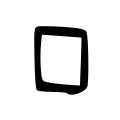
\includegraphics[width=1.5em]{Chapter2/OBI丁.png}}}})
    % 4th Heavenly Stem; nail
    {\large{\textbf{teṅ}}}, 
    \textit{teṅ}  `4th Heavenly Stem`, \textcolor{gray}{\textit{ṭeaṅ} `clang'}
\end{flushleft}
   

    % 09-11/0833e
%    \item {\Large{頂}} % 丁 + 頁
%    {\large{{\textsuperscript{fac}}teṅ}},
%    \textit{teṅX} `top, apex; to carry on the head`

    % 09-11/0833f
%    \item {\Large{汀}} % 丁 + 氵
%    {\large{{\textsuperscript{aq}}teṅ}}
%    \textit{theṅ} `sandbank, shore`

    % 09-11/0833g
%    \item {\Large{町}} % 丁 + 田
%    {\large{{\textsuperscript{agr}}teṅ}},
%    \textit{deṅX, theṅX}
%    `village block, small settlement`

    % 09-11/0833h
%    \item {\Large{亭}} % 丁 + high roof
%    {\large{{\textsuperscript{pav}}teṅ}}, \textit{deṅX}
%    `pavilion, kiosk`
%\begin{itemize}
    % 09-11/0833i
%    \item {\Large{停}} % 亻 + 亭
%    {\large{{\textsuperscript{hom}}deṅ}}, \textit{deṅ}
%    `to stop, pause`
%\end{itemize}

    % 09-11/0833j
    \item    \begin{flushleft} 
    {\Large{正}} (pre-Qin  \hspace{-0.5em} \makebox[1.2em][l]{{\raisebox{-0.1em}{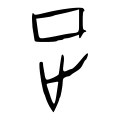
\includegraphics[width=1.5em]{Chapter2/OBI正.png}}}}) % 一 + 止
    {\large{{\textsuperscript{ped}}teṅ}},
    \textit{cieṅ, cieṅH}
    `upright` \end{flushleft}
%\begin{itemize}
    % 09-11/0833o
%    \item {\Large{征}} % 彳 + 正
%    {\large{{\textsuperscript{step}}cieṅ}}, \textit{cieṅ}
%    `to go on a campaign or expedition`

    % 09-11/0833r
%    \item {\Large{政}} % 攵 + 正
%    {\large{{\textsuperscript{act}}cieṅ}}, \textit{cieṅH}
%    `government, adminisṭation`

    % 09-11/0833t
%    \item {\Large{整}} % 攵 + 正
%    {\large{{\textsuperscript{act}}cieṅ}}, \textit{cieṅX}
%    `to arrange, put in order`

    % 09-11/0833u
%    \item {\Large{証}} % 訁 + 正
%    {\large{{\textsuperscript{dic}}cieṅ}}, \textit{cieṅH}
%    `proof, evidence, testimony`

    % 09-11/0833v
%    \item {\Large{鉦}} % 金 + 正
%    {\large{{\textsuperscript{met}}cieṅ}}, \textit{cieṅ}
%    `a small gong`

    % 09-11/0833y
    %\item {\Large{竀}} % 立 + 争
    %{\large{{\textsuperscript{stand}}ṭhieṅ}},
    %\textit{ṭhieṅ}
    %`rare, archaic (possibly "to rise/strive")`

    % 09-11/0833z
%    \item {\Large{定}} % 宀 + 正
%    {\large{{\textsuperscript{tect}}deṅH}},
%    \textit{deṅH, teṅH}
%    `to settle, fix, decide`

    % 09-11/1248b
 %   \item {\Large{綻}} % 糸 + 定
 %   {\large{{\textsuperscript{ser}}dreanH}}, \textit{dreanH}
 %   `to burst open (at the seam), to unravel`
%\end{itemize}
\end{itemize}

%======================================================
    % 09-12
    %======================================================
    % 09-12/0834a

\medskip

    \begin{itemize}
    \item \begin{flushleft} {\Large{鼎}} 
    {\large{\textbf{teṅ}}}, \textit{teṅX}
    `three-legged bronze cauldron` \end{flushleft}

    % 09-12/0834g
    \item \begin{flushleft}  {\Large{鼑}} (later {\Large{貞}})   % 貝 + 正
      {\large{{\textsuperscript{prognosc}}teṅ}}, \textit{ṭieṅ}
    `steadfast` \end{flushleft}
%\begin{itemize}
    % 09-12/0834j
%    \item {\Large{禎}} % 礻 + 貞
%    {\large{{\textsuperscript{sac}}ṭieṅ}}, \textit{ṭieṅ}
%    `auspicious, good omen`

    % 09-12/0834k
%    \item {\Large{偵}} % 亻 + 貞
%    {\large{{\textsuperscript{hom}}ṭhieṅ}},
 %   \textit{ṭhieṅH, ṭieṅ}
 %   `to scout, investigate, spy`

    % 09-12/0834l
 %   \item {\Large{楨}} % 木 + 貞
 %   {\large{{\textsuperscript{arb}}ṭieṅ}}, \textit{ṭieṅ}
 %   `pillar, upright post of wood`

    % 09-12/0834m
 %   \item {\Large{赬}} % 赤 + 丁
 %   {\large{{\textsuperscript{red}}ṭhieṅ}}, \textit{ṭhieṅ}
 %   `scarlet, bright red`
%\end{itemize}
\end{itemize}

\medskip
    %======================================================
    % 09-17
    %======================================================
    % 09-17/0835a
\begin{minipage}{\columnwidth}
\begin{itemize}[leftmargin=*, labelsep=0.5em]  
    \item {\Large{\symbol{135740}}} 
    {\large{teṅ}}, \textit{theṅX}
    `court`

    % 09-17/0835d
    \item {\Large{廷}} % 廴 + 壬/延 
    {\large{{\textsuperscript{progred}}teṅ}},
    \textit{deṅ, deṅH}
    `court`
%\begin{itemize}
    % 09-17/0835h
%    \item {\Large{庭}} % 广 + 廷
%    {\large{{\textsuperscript{bld}}deṅ}},
%    \textit{deṅ, theṅH}
%    `courtyard, yard`

    % 09-17/0835i
%    \item {\Large{挺}} % 扌 + 廷
%    {\large{{\textsuperscript{man}}deṅ}},
%    \textit{deṅX, theṅX}
%    `to straighten, to hold out, to support`

    % 09-17/0835m
%    \item {\Large{霆}} % 雨 + 廷
%    {\large{{\textsuperscript{pluv}}deṅ}}, \textit{deṅ}
%    `thunder`
%\end{itemize}

    % 09-17/0835r
    \item 
   
\includegraphics[width=1.5em]{Chapter2/呈.png} 
    %{\Large{呈}} 
    {\large{{\textsuperscript{or}}teṅ}}, \textit{ḍieṅ}
    `submit`
%\begin{itemize}
     % 09-17/0835s
   % \item {\Large{珵}} % 王 + 廷
   % {\large{{\textsuperscript{gem}}ḍieṅ}},
   % \textit{ḍieṅ} `jade ornament`

    % 09-17/0835t
   % \item {\Large{程}} % 禾 + 呈
   % {\large{{\textsuperscript{cere}}ḍieṅ}}, \textit{ḍieṅ}
   % `journey, distance, measure`

    % 09-17/0835u
  %  \item {\Large{裎}} % 衣 + 呈
  %  {\large{{\textsuperscript{vest}}ḍieṅ}}, \textit{ḍieṅ}
  %  `to sṭip clothing, go partly naked`
%\end{itemize}
\end{itemize}
\end{minipage}

\vspace{8mm}

\begin{minipage}{\columnwidth}
\begin{itemize}[leftmargin=*, labelsep=0.5em]  
    % 09-25
    %======================================================
    % 09-25/0812a
    \item

    \textcolor{gray}{{\Large{生}} {\large{\textbf{ṣeṅ}}}, \textit{ṣaeṅ, ṣiaeṅ} `be born`}


    % 09-25/0812i
    %\item {\Large{眚}} % 目 + 生
    %{\large{{\textsuperscript{ocul}}ṣieṅX}}, \textit{ṣieṅX}
    %`eye disease, impairment of sight`

    % 09-25/0812q
    %\item {\Large{姓}} % 女 + 生
    %{\large{{\textsuperscript{fem}}sieṅH}}, \textit{sieṅH}
    %`surname, family name`

    % 09-25/0812s
    \item {\Large{性}} % 忄 + 生
    {\large{{\textsuperscript{cor}}ṣeṅ}}, \textit{sieṅH}
    `character`

    % 09-25/0812t
   % \item {\Large{狌}} % 犭 + 生
   % {\large{{\textsuperscript{can}}sieṅH}}, \textit{sieṅH}
   % `a wild beast (rare/uncertain)`

    % 09-25/0812u
    %\item {\Large{鼪}} % 鼠 + 生
    %{\large{{\textsuperscript{rod}}sieṅH}}, \textit{sieṅH}
    %`a skunk- or weasel-like creature`

    % 09-25/0812x
    \item {\Large{星}} % 日 + 生
    {\large{{\textsuperscript{sol}}ṣeṅ}},
    \textit{dzieṅ, seṅ}
    `star`
\begin{itemize}

    % 09-25/0812y
%    \item {\Large{曐}} % 日 + 星
%    {\large{{\textsuperscript{sol}}seṅ}}, \textit{seṅ}
 %   `variant form of "star"`

    % 09-25/0812z
 %   \item {\Large{猩}} % 犭 + 星
  %  {\large{{\textsuperscript{can}}seṅ}},
 %   \textit{seṅ, ṣaeṅ}
  %  `ape with red fur (orangutan)`

    % 09-25/0812a'
    \item {\Large{腥}} % 月(肉) + 星
    {\large{{\textsuperscript{carn}}seṅ}},
    \textit{seṅ, seṅH}
    `fishy smell`

    % 09-25/0812b'
    \item {\Large{醒}} % 酉 + 星
    {\large{{\textsuperscript{vin}}seṅ}},
    \textit{seṅ, seṅH, seṅX}
    `sober up`

\end{itemize}
\end{itemize}
\end{minipage}
\end{multicols}

\paragraph{The -\textit{uwṅ}/-\textit{iəwṅ} \textit{xiéshēng} rime pair.}
\label{par:uwng-iəwṅ-XS-pair}
The following \textit{xiéshēng} series pairs the Middle Chinese type A rime -\textit{uwṅ} (O-I-東-\textsc{oriens}-smooth) and the Middle Chinese type B rime -\textit{iəwṅ} (C-III-鐘-\textsc{calix}-smooth). 


\begin{itemize}
    \item {\Large{龍}} % 12-15/1193a
    {\large{\textbf{luwṅ}}},
    \textit{liəwṅ},  {\color{gray}{\textit{maewṅ}}} `dragon' % 1193a

    \item {\Large{壟}} % 12-15/1193f
    {\large{{\textsuperscript{terr}}luwṅ}},
    \textit{liəwṅX} `burial mound' % 1193f

    \item {\Large{隴}} % 12-15/1193g
    {\large{{\textsuperscript{tum}}luwṅ}},
    \textit{liəwṅX} 
    name of mountain range  % 1193g

    \item {\Large{蘢}} % 12-15/1193h
    {\large{{\textsuperscript{herb}}luwṅ}},
    \textit{liəwṅ, luwṅ} `water-pepper' % 1193h

    \item {\Large{龐}} % 12-15/1193i
    {\large{{\textsuperscript{lax}}luwṅ}},
    \textit{luwṅ} `imposing' % 1193i

    \item {\Large{礱}} % 12-15/1193k
    {\large{{\textsuperscript{lap}}luwṅ}},
    \textit{luwṅ} `grind' % 1193k

    \item {\Large{籠}} % 12-15/1193l
    {\large{{\textsuperscript{bamb}}luwṅ}},
    \textit{luwṅ, luwṅX, liəwṅ} `bamboo crate' % 1193l

    \item {\Large{聾}} % 12-15/1193m
    {\large{{\textsuperscript{aur}}luwṅ}},
    \textit{luwṅ} `deaf' % 1193m

    \item {\Large{蠪}} % 12-15/1193o
    {\large{{\textsuperscript{serp}}luwṅ}},
    \textit{luwṅ} `giant ant' % 1193o

    \item {\Large{寵}} % 12-15/1193p
    {\large{{\textsuperscript{tect}}luwṅ}},
    \textit{ṭhiəwṅX} `favor' (v.) % 1193p
\end{itemize}

Here is a selection of those \textit{xiéshēng} series with other initials that pair -\textit{uwṅ} (O-I-東-\textsc{oriens}-smooth) and the -\textit{iəwṅ} (C-III-鐘-\textsc{calix}-smooth). 


\begin{multicols}{2}
\raggedcolumns


\begin{itemize}
    %======================================================
    % 12-01
    %======================================================
    % 12-01/1172a
    \item {\Large{工}}
    {\large{\textbf{kuwṅ}}}, \textit{kuwṅ}
    `work`

    % 12-01/1172d
   % \item {\Large{功}} % 力 + 工
    %{\large{\textsuperscript{for}kuwṅ}}, \textit{kuwṅ}
    %`achievement, merit`

    % 12-01/1172e
   % \item {\Large{攻}} % 攵 + 工
    %{\large{\textsuperscript{act}kuwṅ}}, \textit{kuwṅ}
    %`to attack, assault`

    % 12-01/1172g
    %\item {\Large{貢}} % 貝 + 工
    %{\large{\textsuperscript{conch}kuwṅ}}, \textit{kuwṅH}
    %`tribute, offering`

    % 12-01/1172h
  %  \item {\Large{空}} % 穴 + 工
    %{\large{\textsuperscript{cav}kuwṅ}}, \textit{khuwṅ, khuwṅH}, \textit{khuwṅX}
    %`empty`

%\begin{itemize}
  % 12-01/1172z
%    \item {\Large{悾}} % 心 + 空(工)
    %{\large{\textsuperscript{card}kuwṅ}}, \textit{khaewṅ},  \textit{khuwṅ}, \textit{khuwṅH}
    %`honest, openhearted (rare)`

    % 12-01/1172a'
    %\item {\Large{控}} % 扌 + 空
    %{\large{\textsuperscript{man}\textit{khaewṅH}}}, \textit{khuwṅH}
    %`to control, restrain`

    % 12-01/1172b'
   % \item {\Large{椌}} % 木 + 空
    %{\large{\textsuperscript{arb}\textit{khaewṅ}}}, \textit{khaewṅ}
    %`name of a tree or wooden utensil (rare)`

%\end{itemize}

    % 12-01/1172i
   % \item {\Large{紅}} % 糸 + 工
    %{\large{\textsuperscript{ser}kuwṅ}}, \textit{ḫuwṅ}
    %`red`

    % 12-01/1172j
%    \item {\Large{虹}} % 虫 + 工
    %{\large{\textsuperscript{serp}ḫuwṅ}}, \textit{ḫuwṅ, kaewṅH}
    %`rainbow`

    % 12-01/1172k
  %  \item {\Large{訌}} % 言 + 工
    %{\large{\textsuperscript{dic}ḫuwṅ}}, \textit{ḫuwṅ}
    %`dispute, argue (archaic)`

    % 12-01/1172l
 %   \item {\Large{䲨}} % (fish radical?) + 工
    %{\large{\textsuperscript{av}ḫuwṅ}}, \textit{ḫuwṅ}
   % `a type of fish (rare)`

%\begin{itemize}

 % 12-01/1172g'
 %   \item {\Large{鴻}} % 鳥 + 工
    %{\large{\textsuperscript{av}\textit{ḫuwṅ}}}, \textit{ḫuwṅ}
    %`wild goose; vast, great`

%\end{itemize}

    % 12-01/1172m
%    \item {\Large{��}} % 足 + 工
    %{\large{\textsuperscript{pod}\textit{ḫuwṅ}}}, \textit{ḫuwṅ}
    %`archaic form (foot-related)`

    % 12-01/1172p
    \item {\Large{\symbol{"28F8A}}} % 忄 + 工
    {\large{\textsuperscript{passer}kuwṅ}}, \textit{kiəwṅX}
    `swan`

    % 12-01/1172s
    %\item {\Large{邛}} % 邑 + 工
    %{\large{\textsuperscript{civ}\textit{giəwṅ}}}, \textit{giəwṅ}
    %`place name, Qiong (ancient region)`

    % 12-01/1172u
    %\item {\Large{杠}} % 木 + 工
    %{\large{\textsuperscript{arb}\textit{kaewṅ}}}, \textit{kaewṅ}
    %`wooden bar, pole`

    % 12-01/1172v
 %   \item {\Large{江}} % 氵 + 工
    %{\large{\textsuperscript{aq}\textit{kaewṅ}}}, \textit{kaewṅ}
    %`river (Yangtze-like)`

    % 12-01/1172x
  %  \item {\Large{矼}} % 石 + 工
    %{\large{\textsuperscript{lap}\textit{kaewṅ}}}, \textit{khuwṅH}
    %`stone mortar or block (rare)`

    % 12-01/1172y
   % \item {\Large{項}} % 頁 + 工
    %{\large{\textsuperscript{fac}\textit{ḫaewṅX}}}, \textit{ḫaewṅX}
    %`nape of the neck, item`

    %\item {\Large{\symbol{"2201C}}}  
%{\large{\textsuperscript{ten}kuwṅ}}, \textit{kiəwṅX}
%  `embrace'
  
%\begin{itemize}

    % 12-01/1172c'
%    \item {\Large{鞏}} 
    %{\large{\textsuperscript{lea}kiəwṅ}}, \textit{kiəwṅX}
    %`to strengthen, secure`

    % 12-01/1172d'
    %\item {\Large{恐}} % 心 + 工
    %{\large{\textsuperscript{cor}khiəwṅ}}, \textit{khiəwṅX}
    %`fear, dread`

    % 12-01/1172e'
    %\item {\Large{蛩}} % 虫 + 工
    %{\large{\textsuperscript{serp}giəwṅ}}, \textit{giəwṅ}
    %`cricket (insect)`

    % 12-01/1172f'
  %  \item {\Large{跫}} % 足 + 工
    %{\large{\textsuperscript{ped}giəwṅ}}, \textit{giəwṅ}, \textit{khaewṅ}
    %`sound of footsteps`
%\end{itemize}


   
\end{itemize}

\medskip

\begin{itemize}
  % 12-03/1182a
  \item {\Large{廾}} % 12-03/1182a
    {\large{\textbf{kuwṅ}}},
    \textit{kiəwṅX} `salute with raised hands' % 1182a

  % 12-03/1182g
  %\item {\Large{龏}} % 12-03/1182g
    %{\large{{\textsuperscript{dracon}}kuwṅ}},
  %  \textit{kiəwṅ} `reverent' % 1182g

  % 12-03/1182l
 % \item {\Large{恭}} % 12-03/1182l
    %{\large{{\textsuperscript{cor}}kuwṅ}},
 %   \textit{kiəwṅ} `reverent' % 1182l

  % 12-03/1182o
 % \item {\Large{洪}} % 12-03/1182o
    %{\large{{\textsuperscript{aq}}kuwṅ}},
 %   \textit{ḫuwṅ} `deluge' % 1182o

  % 12-03/1182r
  \item {\Large{烘}} % 12-03/1182r
    %{\large{{\textsuperscript{ign}}kuwṅ}},
    \textit{huwṅ} `roast' % 1182r
\end{itemize}

\medskip

\begin{minipage}{\columnwidth}
\begin{itemize}[leftmargin=*, labelsep=0.5em]  
    \item {\Large{雍}} 
    {\large{\textbf{'uwṅ}}},
 \textit{'iəwṅ}, \textit{'iəwṅX}
 `placid'  % 0718a

    \item {\Large{甕}} % 03-20/0718h
    {\large{{\textsuperscript{teg}}'uwṅ}},
      \textit{'uwṅH} 
`urn' % 0718h
\end{itemize}
\end{minipage}

\bigskip
\bigskip


\begin{itemize}
    \item {\Large{重}} 
    {\large{\textbf{tuwṅ}}},
 \textit{ḍiəwṅg} `double', \textit{ḍiəwṅX}
 `heavy', \textit{ḍiəwṅH} `weigh'  % 0718a

    \item {\Large{動}} % 03-20/0718h
    {\large{{\textsuperscript{virt}}tuwṅ}},
      \textit{duwṅX} 
`move' % 0718h

\end{itemize}

\medskip



\begin{itemize}
    \item \begin{flushleft}   {\Large{縱}}     {\large{{\textsuperscript{ser}}tsuwṅ}},
 \textit{tsiəwṅH} `loosen',  \textit{tsiəwṅ} `vertical'     \end{flushleft}


    \item {\Large{豵}}  
    {\large{{\textsuperscript{porc}}tsuwṅ}},
   \textit{tsuwṅ} `shoat' % 0718h

\end{itemize}


\begin{itemize}
    \item \begin{flushleft}   {\Large{奉}}     {\large{{\textsuperscript{ser}}puwṅ}},
 \textit{biəwṅX} `offer'    \end{flushleft}


    \item {\Large{唪}}  
    {\large{{\textsuperscript{or}}tsuwṅ}},
   \textit{buwṅ} `intone' % 0718h

\end{itemize}


%奉 bjowngX offer
%buwngX
%唪 buwngX
%ADD SOME FROM OTHER INITIALS
\end{multicols}


\subparagraph{A poorly behaved series that includes  -\textit{əwṅ} readings.}
The series built on 
農 % 15-09/1005a
    \textit{nəwṅ} `agriculture' offers the type A rimes 
-\textit{əwṅ} and -\textit{uwṅ}, with the former predominating, and it offers the type B rime   
-\textit{iəwṅ}. In deference to its type B reading, I discuss it here.  

%15-09

 %   15-09/1005a 農 nəwṅ
 %   15-09/1005b 辳 nəwṅ
 %   15-09/1005g 噥 nəwṅ
 %   15-09/1005h 膿 nəwṅ
 %   15-09/1005i 濃 ṇiəwṅ, nuwṅ
 %   15-09/1005j 醲 ṇiəwṅ, nuwṅ
 %   15-09/1005k 穠 ṇiəwṅ, ñiəwṅ
 %   15-09/1005l 襛 ṇiəwṅ, ñiəwṅ
 %   15-09/1005- �� ṇiəwṅ
 %   15-09/1005- 齈 nuwṅH

\begin{itemize}
    \item {\Large{農}} % 15-09/1005a
    {\large{\textbf{nəwṅ}}},
    \textit{nəwṅ} `agriculture' % 1005a

    \item {\Large{噥}} % 15-09/1005g
    {\large{{\textsuperscript{or}}nəwṅ}},
    \textit{nəwṅ} `garrulous' % 1005g

    \item {\Large{膿}} % 15-09/1005h
    {\large{{\textsuperscript{carn}}nəwṅ}},
    \textit{nəwṅ} `pus' % 1005h

    \item {\Large{濃}} % 15-09/1005i
    {\large{{\textsuperscript{aq}}nəwṅ}},
    \textit{ṇiəwṅ, nuwṅ} `concentrated' (of a liquid) % 1005i

    %\item {\Large{醲}} % 15-09/1005j
    %{\large{{\textsuperscript{vin}}nəwṅ}},
    %\textit{ṇiəwṅ, nuwṅ} `concentrated' (of a liquid) % 1005j

    \item {\Large{穠}} % 15-09/1005k
    {\large{{\textsuperscript{gran}}nəwṅ}},
    \textit{ṇiəwṅ, ñiəwṅ} `lush' % 1005k

   % \item {\Large{襛}} % 15-09/1005l
    %{\large{{\textsuperscript{vest}}nəwṅ}},
    %\textit{ṇiəwṅ, ñiəwṅ} `rich or thick garment (?)' % 1005l

 %   \item {\Large{\symbol{"2844A}}} % 15-09/1005- (unreadable)
    %{\large{{\textsuperscript{???}}nəwṅ}},
   % \textit{ṇiəwṅ} `???' % 1005-

    \item {\Large{齈}} % 15-09/1005- or 1005l?
    {\large{{\textsuperscript{nas}}nəwṅ}},
    \textit{nuwṅH} `snot' % 1005-
\end{itemize}

As far as I have been able to determine, this pattern is unique to this one series. It would certainly be imprudent to reconstruct a distinct nuclear vowel in Old Chinese for the rhyme pattern -\textit{əwṅ} / \textit{iəwṅ}, and indeed, this is not necessary because an explanation is to hand.
The 廣韻 \textit{Guǎngyùn} of 1008 is our major source for Middle Chinese readings of characters. This works attempts to faithfully reproduce the phonology of the 601 \textit{Qièyùn}, but of course many changes had affected the pronunciation of Chinese in the meantime. In particular, the Middle Chinese type A rimes 
-\textit{uwṅ} (O-I-東-\textsc{oriens}-smooth) and -\textit{əwṅ}  (C-I-冬-\textsc{hiems}-smooth) were no longer distinguished. The merger of -\textit{uwṅ} and  -\textit{əwṅ} is explicitly indicated in the 四聲等子 \textit{Sìshēng Děngzǐ}, which was roughly contemporaneous with the \textit{Guǎngyùn}  
\citep[pp. 183 and 185]{shen2020phonological}. 
Thus, we are entitled to speculate that 
農 \textit{nəwṅ} `agriculture',
噥 \textit{nəwṅ} `garrulous', and 
膿 \textit{nəwṅ} `pus' were inherted belonging to the -\textit{uwṅ} rime and that the authors of the \textit{Guǎngyùn} incorrectly placed these words under -\textit{əwṅ}. 

THINGS TO DO: 

\begin{itemize}
    \item CHECK GUANYUN
    \item CHECK EARLIER VERSION OF THE QIEYUN
    \item CHECK THE BEHAVRIOR OF THESE THREE WORDS IN TERMS OF THEIR RHYMES
\end{itemize}

\paragraph{\textit{Xiéshēng} series with type B readings in rime -\textit{iuwṅ}.}
\label{par:əwṅ-iuwṅ-XS-pair}
%5 Nothing for -u-, except sort of this one: 
%
%    15-02/1015a 降 ḫaewṅ, kaewṅH
%    15-02/1015d 洚 ḫaewṅ, ḫəwṅ, huwṅ, kaewṅH
%    15-02/1015e 戇 huwṅH
%    15-02/1015f 隆 liuwṅ
%    15-02/1015g 癃 liuwṅ
%
In the 來 \textit{l}- initial series built on 降 \textit{ḫaewṅ}, \textit{kaewṅH} `descend', there are two type A rimes -\textit{əwṅ} (C-I-冬-\textsc{hiems}-smooth)
and -\textit{uwṅ} (O-I-東-\textsc{oriens}-smooth), because of this complication it would be imprudent to offer a transliteration of the characters before further discussion. 

\begin{itemize}
    \item  {\color{gray}{ {\Large{降}} % 15-02/1015a
   % {\large{\textbf{ḫəwṅ}}},
    \textit{ḫaewṅ, kaewṅH} `descend'}} % 1015a

    \item {\Large{洚}} % 15-02/1015d
    %{\large{{\textsuperscript{aq}}ḫəwṅ}},
    {\color{gray}{\textit{ḫaewṅ, kaewṅH,}}} \textit{ḫəwṅ, ḫuwṅ} `deluge' % 1015d

 \item {\color{gray}{ {\Large{絳}} % 15-02/1015d
    %{\large{{\textsuperscript{ser}}ḫəwṅ}},
    \textit{kaewṅH} `crimson'}} % 1015d

\item {\color{gray}{ {\Large{栙}} % 15-02/1015d
    %{\large{{\textsuperscript{arb}}ḫəwṅ}},
    \textit{ḫaewṅ} `sail batten'  (in 栙双)}} % 1015d




  


%    \item {\Large{戇}} % 15-02/1015e
    %{\large{{\textsuperscript{???}}huwṅH}},
%    \textit{huwṅH} `foolish, crude' % 1015e

    \item {\Large{隆}} % 15-02/1015f
(structurally 
    \makebox[1.25em][l]{\raisebox{-0.2em}{\includesvg[width=1.3em]{Chapter2/隆.svg}}})
    %\symbol{"28F07} 
    %{\large{{\textsuperscript{hill}}liuwṅ}},
    \textit{liuwṅ} `prosperous, elevated' % 1015f
\begin{itemize}
    \item {\Large{癃}} % 15-02/1015g
    %{\large{{\textsuperscript{dis}}liuwṅ}},
    \textit{liuwṅ} `infirm with age' % 1015g
\end{itemize}
\end{itemize}






  


% 窿 liuwng

%Based on this series it is quite hard to know what the type A member of this pair should be. However, when we look at other  initials we see clearly that there is an alternation between type A -\textit{əwṅ} and type B -\textit{iuwṅ}. 

If we look around at \textit{xiéshēng} series beginning with other initials, we see that there are at least four patterns of type A and type B rimes occurring in a single \textit{xiéshēng} series, where the type B rime (possibly among others) is -\textit{iuwṅ} (see Table \ref{tab:type_correspondences}).  



\subparagraph{Type A -\textit{əwṅ} with type B -\textit{iuwṅ}}
\label{subpara:typeA-awng-typeB-iuwng}
The following \textit{xiéshēng} series pairs the Middle Chinese type A rime -\textit{əwṅ} (C-I-冬-\textsc{hiems}-smooth) and the Middle Chinese type B rime -\textit{iuwṅ} (O-III-東-\textsc{oriens}-smooth).

\medskip

%    15-03/1002a 冬 təwṅ
%    15-03/1002e 終 ciuwṅ
%    15-03/1002f 螽 ciuwṅ

\begin{multicols}{2}
\raggedcolumns
\begin{itemize}
    \item {\Large{冬}} % 15-03/1002a
    %{\large{\textbf{təwṅ}}},
    \textit{təwṅ} `winter' % 1002a

    \item {\Large{終}} % 15-03/1002e
    %{\large{{\textsuperscript{ser}}təwṅ}},
    \textit{ciuwṅ} `end' % 1002e

    \item {\Large{螽}} % 15-03/1002f
    %{\large{{\textsuperscript{serp}}təwṅ}},
    \textit{ciuwṅ} `bush crickets' % 1002f
\end{itemize}

\medskip
%15-04

%    15-04/1010a 眾 ciuwṅH
%    15-04/1010e �� ciuwṅ
%    15-04/1010f 潨 dzəwṅ, dzuwṅ, ciuwṅ




\medskip
%15-05

%    15-05/1011a 充 chiuwṅ
%    15-05/1011b 統 thəwṅH


\begin{itemize}

\item {\Large{充}} % 15-05/1011a
  %  {\large{\textbf{chəwṅ}}},
    \textit{chiuwṅ} `fill' % 1011a

    \item {\Large{統}} % 15-05/1011b
    %{\large{{\textsuperscript{ser}}chəwṅ}},
    \textit{thəwṅH} `guiding thread' % 1011b
\end{itemize}

\bigskip 

 %   15-13/1003a 宗 tsəwṅ
  %  15-13/1003f 綜 tsəwṅH
   % 15-13/1003g 琮 dzəwṅ
   % 15-13/1003h 崇 dẓiuwṅ

\begin{minipage}{\columnwidth}
\begin{itemize}[leftmargin=*, labelsep=0.5em]  
\item {\Large{宗}} % 15-13/1003a
 %   {\large{\textbf{tsəwṅ}}},
    \textit{tsəwṅ} `ancestral hall' % 1003a

    \item {\Large{綜}} % 15-13/1003f
    %{\large{{\textsuperscript{ser}}tsəwṅ}},
    \textit{tsəwṅH} `heddle' % 1003f

    \item {\Large{琮}} % 15-13/1003g
    %{\large{{\textsuperscript{gem}}tsəwṅ}},
    \textit{dzəwṅ} `hollow jade prism' % 1003g

    \item {\Large{崇}} % 15-13/1003h
    %{\large{{\textsuperscript{mon}}tsəwṅ}},
    \textit{dẓiuwṅ} `lofty' % 1003h
\end{itemize}
\end{minipage}

\medskip

%    15-08/1008a 肜 yiuwṅ
%    15-08/1008c 彡 yiuwṅ
%    15-08/1008e 彤 duṅ

% ==========================
% 15-08
% ==========================

\begin{itemize}
  \item {\Large{彡}} % 15-08/1008c
   % {\large{\textbf{yuṅ}}},
    \textit{yiuwṅ} `second-day sacrifice' % 1008c
  
  \item {\Large{肜}} % 15-08/1008a
    %{\large{{\textsuperscript{carn}}yuṅ}},
    \textit{yiuwṅ} `second-day sacrifice' % 1008a


  \item {\Large{彤}} % 15-08/1008e
    %{\large{{\textsuperscript{cinnibar}}yuṅ}},
    \textit{dəwṅ} `vermilion' % 1008e
\end{itemize}
\end{multicols}

\subparagraph{Type A -\textit{uwṅ} and -\textit{əwṅ} with type B -\textit{iuwṅ}.}
\label{subpara:typeA-uwng-awng-typeB-iuwng}
The following \textit{xiéshēng} series pairs the Middle Chinese type A rimes 
\textit{uwṅ} (O-I-東-\textsc{oriens}-smooth) and -\textit{əwṅ}  (C-I-冬-\textsc{hiems}-smooth) and the Middle Chinese type B rime -\textit{iuwṅ} (O-III-東-\textsc{oriens}-smooth).
The series built on 降 
    \textit{ḫaewṅ, kaewṅH} `descend', which opened the discussion in this paragraph, also belongs to this type. 

    


%    15-04/1010a 眾 ciuwṅH
%    15-04/1010e �� ciuwṅ
%    15-04/1010f 潨 dzəwṅ, dzuwṅ, ciuwṅ

%    15-02/1015d 洚 ḫaewṅ, ḫəwṅ, ḫuwṅ, kaewṅH
%    15-02/1015e 戇 huwṅH
%    15-02/1015f 隆 liuwṅ

%    15-04/1010e �� ciuwṅ
%    15-04/1010f 潨 dzəwṅ, dzuwṅ, ciuwṅ

%In transliterating this next one, since two type A readings appear even with one character, I have no but to transliterate with the type B reading.  


\begin{table}[tbp]
    \centering
    \begin{tabular}{ll|ll|l}
        \hline
         \multicolumn{2}{c}{\textbf{Type A}} & \multicolumn{2}{c}{\textbf{Type B}} & \textbf{Reference} \\
        \hline
        \textit{əwṅ}  &  & \textit{iuwṅ}  &  & §\ref{subpara:typeA-awng-typeB-iuwng} \\
        \textit{uwṅ},  & \textit{əwṅ}  & \textit{iuwṅ}  &  & §\ref{subpara:typeA-uwng-awng-typeB-iuwng} \\
        \textit{uwṅ}  &  & \textit{iuwṅ},  & \textit{iəwṅ}  & §\ref{subpara:typeA-uwng-typeB-iuwng-iewng} \\
        \textit{uwṅ}  &  & \textit{iuwṅ}, &   \textit{iəm}  & §\ref{subpara:typeA-uwng-typeB-iuwng-iem} \\
        \hline
    \end{tabular}
    \caption{Rime patterns in 
    \textit{xiéshēng} series with type B readings in rime -\textit{iuwṅ}}
    \label{tab:type_correspondences}
\end{table}



\medskip

\begin{multicols}{2}
\raggedcolumns
\begin{minipage}{\columnwidth}
\begin{itemize}[leftmargin=*, labelsep=0.5em]  
  % 15-04/1010a
  \item {\Large{眾}} % 15-04/1010a
 %   {\large{ciuwṅ}},
    \textit{ciuwṅH} `crowd, multitude' % 1010a

  % 15-04/1010e (the glyph "��" is unknown)
  \item {\raisebox{-0.1em}{
\includegraphics[width=1.5em]{Chapter2/⿰虫衆.png}} 
%  \Large{\symbol{161860}}
} % 15-04/1010e
    %{\large{{\textsuperscript{serp}}ciuwṅ}},
    \textit{ciuwṅ} `bush crickets' % 1010e

  % 15-04/1010f
  \item  \begin{flushleft}
      
 {\Large{潨}} % 15-04/1010f
    %{\large{{\textsuperscript{aq}}ciuwṅ}},
    \textit{dzəwṅ, dzuwṅ},  `confluence', \textit{ciuwṅ} `riverbank' % 1010f
  \end{flushleft}

\end{itemize}
\end{minipage}
\end{multicols}

\subparagraph{Type A -\textit{uwṅ} with type B -\textit{iuwṅ} and
-\textit{iəwṅ}.}
\label{subpara:typeA-uwng-typeB-iuwng-iewng}
The following \textit{xiéshēng} series pairs the Middle Chinese type A rime -\textit{uwṅ} (O-I-東-\textsc{oriens}-smooth) and the Middle Chinese type B rimes -\textit{iuwṅ} (O-III-東-\textsc{oriens}-smooth) and -\textit{iəwṅ} (C-III-鐘-\textsc{calix}-smooth).

\begin{minipage}{\columnwidth}
\begin{itemize}[leftmargin=*, labelsep=0.5em]  
  % 12-13/1173a
  \item {\Large{公}} % 12-13/1173a
%    {\large{\textbf{kuwṅ}}},
    \textit{kuwṅ} `public' % 1173a

  % 12-13/1190a
  \item {\Large{松}} % 12-13/1190a
    %{\large{{\textsuperscript{arb}}kuwṅ}},
    \textit{ziəwṅ} `pine tree' % 1190a

  % 12-13/1190f
  \item {\Large{崧}} % 12-13/1190f
    %{\large{{\textsuperscript{mon}}kuwṅ}},
    \textit{siuwṅ} `lofty' % 1190f
\end{itemize}
\end{minipage}

\bigskip 

\subparagraph{Type A -\textit{uwṅ} with type B -\textit{iuwṅ} and -\textit{iəm}.} 
\label{subpara:typeA-uwng-typeB-iuwng-iem}
The following \textit{xiéshēng} series pairs the Middle Chinese type A rime -\textit{uwṅ} (O-I-東-\textsc{oriens}-smooth) and the Middle Chinese type B rimes -\textit{iuwṅ} (O-III-東-\textsc{oriens}-smooth) and  -\textit{iəm} (O-III-凡-\textsc{mundanus}-smooth).

\medskip

%    36-26/0625a 凡 biəm
%    36-26/0625b 芃 buwṅ
%    36-26/0625d 帆 biəm
%    36-26/0625e 軓 biəmX
%    36-26/0625f 汎 biuwṅ, phiəmH
%    36-26/0625h 風 piuwṅ, piuwṅH
%    36-26/0625i 飌 piuwṅ
%    36-26/0625j 鳳 biuwṅH
%    36-26/0625n 楓 piuwṅ
%    36-26/0625o 諷 piuwṅH
%    36-26/0625p 渢 biuwṅ

% ==========================
% 36-26 (peculiar series)
% ==========================

\begin{itemize}
  \item {\Large{凡}} % 36-26/0625a
   % {\large{puwṅ}},
    \textit{biəm} `ordinary' % 0625a

  \item {\Large{芃}} % 36-26/0625b
    %{\large{{\textsuperscript{herb}}puwṅ}},
    \textit{buwṅ} `lush' % 0625b

  \item {\Large{帆}} % 36-26/0625d
    %{\large{{\textsuperscript{lint}}puwṅ}},
    \textit{biəm} `sail' (n.) % 0625d

  \item {\Large{軓}} % 36-26/0625e
    %{\large{{\textsuperscript{vehi}}puwṅ}},
    \textit{biəmX} 
    `crossbar' (of a chariot) % 0625e

  \item {\Large{汎}} % 36-26/0625f
    %{\large{{\textsuperscript{aq}}puwṅ}},
    \textit{biuwṅ, phiəmH} `float' % 0625f

  \item {\Large{鳳}} % 36-26/0625j
    %{\large{{\textsuperscript{av}}puwṅ}},
    \textit{biuwṅH} `phoenix' % 0625j

  \item {\Large{風}} % 36-26/0625h
    %{\large{{\textsuperscript{vent}}puwṅ}},
    \textit{piuwṅ, piuwṅH} `wind' % 0625h
\begin{itemize}
  \item {\Large{飌}} % 36-26/0625i
    %{\large{{\textsuperscript{ciconia}}puwṅ}},
    \textit{piuwṅ} `wind' (esp. personified)% 0625i



  \item {\Large{楓}} % 36-26/0625n
    %{\large{{\textsuperscript{arb}}puwṅ}},
    \textit{piuwṅ} `maple' % 0625n

  \item {\Large{諷}} % 36-26/0625o
    %{\large{{\textsuperscript{dic}}puwṅ}},
    \textit{piuwṅH} `satirize' % 0625o

  \item {\Large{渢}} % 36-26/0625p
    %{\large{{\textsuperscript{aq}}puwṅ}},
    \textit{biuwṅ} `whoosh' % 0625p
\end{itemize}
\end{itemize}

\subparagraph{Analyzing \textit{xiéshēng} series with type B readings in rime -\textit{iuwṅ}.}
In analyzing the the four patterns looked at in this paragraph, we can first off allow ourselves to postpone consideration of the fourth pattern (type A -\textit{uwṅ} with type B -\textit{iuwṅ} and -\textit{iəm}), since -\textit{iəm} should be considered together with other rimes that end in -\textit{m} (CROSSREF). Turning to the other three, I have been able to offer five examples of the first pattern (type A -\textit{əwṅ} with type B -\textit{iuwṅ}), versus only two of the second (type A -\textit{uwṅ} and -\textit{əwṅ} with type B -\textit{iuwṅ}) and one of the third (type A -\textit{uwṅ} with type B -\textit{iuwṅ} and
-\textit{iəwṅ}).  Thus, there is a prima facie case for regarding the first pattern as the major phenomenon and explaining the second and third as minor complications. This is indeed possible.  
The \textit{Guǎngyùn} of 1008 is our major source for Middle Chinese readings of characters. This works attempts to faithfully reproduce the phonology of the 601 \textit{Qièyùn}, but of course many changes had affected the pronunciation of Chinese the meantime. In particular, the Middle Chinese type A rimes 
\textit{uwṅ} (O-I-東-\textsc{oriens}-smooth) and -\textit{əwṅ}  (C-I-冬-\textsc{hiems}-smooth) were no longer distinguished. This merger is explicitly indicated in the 四聲等子 \textit{Sìshēng Děngzǐ}, which was roughly contemporaneous with the \textit{Guǎngyùn}  
\citep[pp. 183 and 185]{shen2020phonological}


%\begin{quote}
%The Sìshēng Děngzǐ 四聲等子

%The \textit{Sìshēng Děngzǐ} (see Figure 4.2) mentions 206 rhymes of the \textit{Guǎngyùn} 廣 韻. It is likely that the surviving version was made after 1008, the publication date of the \textit{Guǎngyùn}. However, because characters and categorical features can be replaced when revised, the original version of the \textit{Sìshēng Děngzǐ} was not necessarily produced after the \textit{Guǎngyùn} or the \textit{Jíyùn} 集韻. The \textit{Sìshēng Děngzǐ} contains twenty tables, which reflects the mergers of certain rhymes of the \textit{Qièyùn} 切韻. For instance, in the \textit{Yùnjìng} 韻鏡, the \textit{dōng} 東 rhyme makes up one table, and the \textit{dōng} 冬 and \textit{zhōng} 鍾 rhymes together compose another table. But in the \textit{Sìshēng Děngzǐ}, \textit{dōng} 東, \textit{dōng} 冬, and \textit{zhōng} 鍾 rhymes are combined and listed in the same table.  
%\end{quote}

%\citet[pp. 183 and 185]{shen2020phonological}
%Shan 2020, p. 183 and 185

%I think Ziche said something that also implies that this was already something in the Qieyun.

The upshot is that I can take it as -\textit{əwṅ} / - \textit{iuwṅ} and predict that violations of this pattern are mistakes resulting from a late merger. 

\paragraph{Summmary of \textit{Xiéshēng} rime pairs found after initial 來\textit{l}- in syllables with final -\textit{ṅ}.}
Table \ref{tab:l-XS-rime-pairs-velar-nasal} presents the overall pattern of \textit{Xiéshēng} rime pairs found after initial 來 \textit{l}- in syllables with final -\textit{ṅ}.
Recall that there are no Middle Chinese syllables like *\textit{ləṅ}, with initial 來 \textit{l}- and rime -\textit{əṅ} (O-I-登-\textsc{scando}-smooth), as such the rime -\textit{əṅ} in  Table \ref{tab:l-XS-rime-pairs-velar-nasal} is set in gray. 

It looks from this like we should have five nuclear vowels before the velar nasal in Old Chinese, and it does not feel wild to presume that -\textit{aṅ}/-\textit{iaṅ}   comes from *-aŋ, and -\textit{eṅ}/-\textit{ieṅ}  comes from *-eŋ, but what to reconstruct in the other cases is less obvious. 
For the pair -\textit{əṅ} / -\textit{iṅ} an obvious possibility is that Old Chinese either had *ə that was fronted to -i in type B syllables or that Old Chinese had *-i which was backed to ə in type A syllables. 
The pairs -\textit{uwṅ} / -\textit{iəwṅ} and -\textit{əwṅ} / -\textit{iuwṅ} are mirror images of each other and both involve rounding, so *o or *u are plausible reconstructions for either one, but there is not an obvious mechanism at this juncture for deciding how to allocate the two patterns to the two reconstructed vowels.


 \begin{table}[htbp]
    \centering
    \begin{tabular}{|l|l|l|l|}
    \hline
    \textbf{Type A rime} & \textbf{Type B rime} & & \textbf{OC} \\
    \hline
    -\textit{aṅ}  & -\textit{iaṅ}   & §\ref{par:ang-iang-XS-pair}  & *aŋ \\
    \color{gray}{-\textit{əṅ}} 
    
    & -\textit{iṅ}    & §\ref{par:əng-ing-XS-pair}   & *əŋ or *iŋ ? \\
    -\textit{eṅ}  & -\textit{ieṅ}   & §\ref{par:eng-ieng-XS-pair}  & *eŋ \\
    -\textit{uwṅ} & -\textit{iəwṅ}  & §\ref{par:uwng-iəwṅ-XS-pair} & *oŋ or *uŋ ? \\
    -\textit{əwṅ} & -\textit{iuwṅ}  & §\ref{par:əwṅ-iuwṅ-XS-pair}  & *oŋ or *uŋ ? \\
    \hline
    \end{tabular}
    \caption{Velar‐nasal type A vs.\ type B \textit{xiéshēng} rime pairs after initial 來 \textit{l}-,
    matching the examples in \S\ref{par:ang-iang-XS-pair}--\ref{par:əwṅ-iuwṅ-XS-pair}.}
    \label{tab:l-XS-rime-pairs-velar-nasal}
\end{table}


\subsubsection{\textit{Xiéshēng} rime pairs found after initial 來\textit{l}- in syllables with final -\textit{k}}
\label{subsubsec:xiesheng_l_k}

\paragraph{} 
 There are five patterns of \textit{xiéshēng} rime pairs of rimes ending in -\textit{k} after initial 來 \textit{l}-, namely -\textit{ak}/-\textit{ia} (§\ref{par:ak-iak-XS-pair}),  
-\textit{ək}/-\textit{ik} (§\ref{par:ək-ik-XS-pair})
 -\textit{ek}/-\textit{iek} 
(§\ref{par:ek-iek-XS-pair}), 
-\textit{uwk}/-\textit{iəwk}
(§\ref{par:uwk-iəwk-XS-pair}), and 
-\textit{əwṅ}/-\textit{iuwṅ} 
(§\ref{par:iuwk-XS}), with this last involving some complications. 


\paragraph{The -\textit{ak}/-\textit{iak} \textit{xiéshēng} rime pair.}
\label{par:ak-iak-XS-pair}

The following \textit{xiéshēng} series pairs the Middle Chinese type A rime -\textit{ak} (O-I-唐-\textsc{strata}-checked) and the Middle Chinese type B rime -\textit{iak} (O-III-陽-\textsc{sol}-checked).\footnote{Ths is an exceedingly long series; since its full presentation would only clutter the presentation, I have omitted characters that only multiply examples of the same readings.} 
% secretly *-ak

\begin{itemize}
    \item {\Large{各}} % 02-01/0766a
    {\large{{\textsuperscript{or}}kak}},
    \textit{kak} `each' % 0766a

    \item {\Large{胳}} % 02-01/0766d
    {\large{{\textsuperscript{carn}}kak}},
    \textcolor{gray}{\textit{kaek},} \textit{kak} `upper arm' % 0766d

   % \item {\Large{袼}} % 02-01/0766e
    %{\large{{\textsuperscript{vest}}kak}},
    %\textit{kaek, kak} `sleeve' % 0766e

%    \item {\Large{閣}} % 02-01/0766f
    %{\large{{\textsuperscript{port}}kak}},
    %\textit{kak} `chamber' % 0766f

    \item {\Large{恪}} % 02-01/0766g
    {\large{{\textsuperscript{cor}}kak}},
    \textit{khak} `respectful' % 0766g

    \item {\Large{貉}} % 02-01/0766h
    {\large{{\textsuperscript{best}}kak}},
    \textit{ḫak}, \textcolor{gray}{\textit{maeH, maek}} `raccoon dog' % 0766h

    %\item {\Large{狢}} % 02-01/0766j
    %{\large{{\textsuperscript{can}}kak}},
    %\textit{maek} `raccoon dog' % 0766j

    %\item {\Large{洛}} % 02-01/0766k
    %{\large{{\textsuperscript{aq}}kak}},
    %\textit{lak} a river name  % 0766k

    \item {\Large{烙}} % 02-01/0766n
    {\large{{\textsuperscript{ign}}kak}},
    \textit{lak} `brand' (v.) % 0766n

    \item {\Large{絡}} % 02-01/0766o
    {\large{{\textsuperscript{ser}}kak}},
    \textit{lak} `enmesh' % 0766o

%    \item {\Large{酪}} % 02-01/0766p
    %{\large{{\textsuperscript{vin}}kak}},
    %\textit{lak} `posset' % 0766p
   

%    \item {\Large{雒}} % 02-01/0766q
    %{\large{{\textsuperscript{passer}}kak}},
    %\textit{lak} `owlet' % 0766q
   

%    \item {\Large{\symbol{"2929A}}} % 02-01/0766r
    %{\large{{\textsuperscript{cori}}kak}},
    %\textit{lak} `rawhide' % 0766r

 %   \item {\Large{駱}} % 02-01/0766s
    %{\large{{\textsuperscript{equ}}lak}},
    %\textit{lak} `camel' % 0766s
    % (馬 => “equ” for equine animals)

  %  \item {\Large{鴼}} % 02-01/0766t
    %{\large{{\textsuperscript{avi}}kak}},
    %\textit{lak} `egret' % 0766t

    \item {\Large{珞}} % 02-01/0766u
    {\large{{\textsuperscript{gem}}kak}},
    \textit{lak}, \textcolor{gray}{\textit{lek}} `bead' % 0766u

    \item {\Large{略}} % 02-01/0766v
    {\large{{\textsuperscript{ager}}kak}},
    \textit{liak} `cadastre' % 0766v
    % (畧 => radical 田 ? => "ager'= field

    %\item {\Large{\symbol{"224DC}}} % 02-01/0766x
    %{\large{{\textsuperscript{eo}}kak}},
    %\textit{kaek} `reach up' % 0766x

    \item \textcolor{gray}{{\Large{格}} % 02-01/0766z
    {\large{{\textsuperscript{arb}}kak}},
    \textit{ḫaek, kaek} `reach up' % 0766z
    }

    %\item {\Large{觡}} % 02-01/0766b'
    %{\large{{\textsuperscript{corn}}kak}},
    %\textit{kaek} `antlers' % 0766b'

%    \item {\Large{骼}} % 02-01/0766c'
    %{\large{{\textsuperscript{oss}}kak}},
    %\textit{kaek, kak, khaeH} `skeleton' % 0766c'

    %\item {\Large{垎}} % 02-01/0766g'
    %{\large{{\textsuperscript{terr}}kak}},
%    \textit{ḫaek} `arid land' % 0766g'

    %\item {\Large{詻}} % 02-01/0766h'
    %{\large{{\textsuperscript{dic}}kak}},
    %\textit{ṅaek} `forcefully assert' % 0766h'

    \item \textcolor{gray}{{\Large{頟}} % 02-01/0766j'
    {\large{{\textsuperscript{fac}}kak}},
    \textit{ṅaek} `forehead'} % 0766j'
   

%    \item {\Large{賂}} % 02-01/0766k'
    %{\large{{\textsuperscript{conch}}kak}},
    %\textit{luH} `bribe' % 0766k'
 

    \item \textcolor{gray}{{\Large{輅}} % 02-01/0766n'
    {\large{{\textsuperscript{rot}}kak}},
    \textit{ḫaek, luH, ṅaeH} `chariot shaft'} % 0766n'
    % (車 => “rot” for wheel?
\begin{itemize}
\vspace{-1mm}
    \item \textcolor{gray}{{\Large{簵}} % 02-01/0766x'
    {\large{{\textsuperscript{bamb}}kak}},
    \textit{luH} `arrow shaft bamboo'} % 0766x'

\end{itemize}

%\item {\Large{客}} % 02-01/0766d'
    %{\large{{\textsuperscript{tect}}khaek}},
    %\textit{kaek} `guest' % 0766d'

%\begin{itemize}
 %   \item {\Large{喀}} % 02-01/0766o'
    %{\large{{\textsuperscript{or}}khaek}},
    %\textit{khaek} `coughing sound' % 0766o'

    %\item {\Large{愙}} % 02-01/0766p'
    %{\large{{\textsuperscript{cor}}khak}},
    %\textit{khak} `respectful' % 0766p'
%\end{itemize}

%    \item {\Large{落}} % 02-01/0766q'
    %{\large{{\textsuperscript{herb}}kak}},
    %\textit{lak} `decline' (v.) % 0766q'

 \item \textcolor{gray}{{\Large{路}} % 02-01/0766l'
    {\large{{\textsuperscript{ped}}kak}},
    \textit{luH} `path'} % 0766l'


\begin{itemize}
\vspace{-2mm}

    \item \textcolor{gray}{{\Large{璐}} % 02-01/0766r'
    {\large{{\textsuperscript{gem}}luH}},
    \textit{luH} `fine jade'} % 0766r'

    \item \textcolor{gray}{{\Large{簬}} % 02-01/0766s'
    {\large{{\textsuperscript{bamb}}luH}},
    \textit{luH} `bamboo hamper'} % 0766s'

%    \item {\Large{露}} % 02-01/0766t'
    %{\large{{\textsuperscript{pluv}}luH}},
    %\textit{luH} `dew' % 0766t'
    

    %\item {\Large{潞}} % 02-01/0766u'
    %{\large{{\textsuperscript{aq}}luH}},
    %\textit{luH} `river name' % 0766u'

    %\item {\Large{鷺}} % 02-01/0766v'
    %{\large{{\textsuperscript{avi}}luH}},
    %\textit{luH} `egret' % 0766v'

\end{itemize}


\end{itemize}

\paragraph{The -\textit{ək}/-\textit{ik} \textit{xiéshēng} rime pair.}
\label{par:ək-ik-XS-pair}

The following \textit{xiéshēng} series pairs the Middle Chinese type A rime 
-\textit{ək} (O-I-登-\textsc{scando}-checked)
and the Middle Chinese type B
rime -\textit{ik}
(O-III-蒸-\textsc{sarmen}-checked). 
%Secretly *-ək


\begin{itemize}
    \item {\Large{力}} % 05-21/0928a
    {\large{lək}},
    \textit{lik} `strength' % 0928a

    \item {\Large{仂}} % 05-21/0928c
    {\large{{\textsuperscript{hom}}lək}},
    \textit{lik, lək} `surplus' % 0928c

    \item {\Large{扐}} % 05-21/0928d
    {\large{{\textsuperscript{man}}lək}},
    \textit{lək} `yarrow-stalk set aside in divination' % 

    \item {\Large{阞}} % 05-21/0928e
    {\large{{\textsuperscript{tum}}lək}},
    \textit{lək} `drainage divide' % 0928e

\begin{itemize}
    \item {\Large{泐}} % 05-21/0928h
    {\large{{\textsuperscript{aq}}lək}},
    \textit{lək} `erosion patterns' % 0928h
\end{itemize}

    \item {\Large{勒}} % 05-21/0928f
    {\large{{\textsuperscript{cori}}lək}},
    \textit{lək} `bridle' % 0928f

  
\end{itemize}


\paragraph{The -\textit{ek}/-\textit{iek} \textit{xiéshēng} rime pair.}
\label{par:ek-iek-XS-pair}
The \textit{xiéshēng} series built on 秝 exhibits only the the Middle Chinese type A rime 
-\textit{ek} (O-IV-青-\textsc{vireo}-checked), and indeed there is no Middle Chinese syllable of the type *\textit{liek}, a fact that will have to be accounted for. 

\begin{itemize}
\setlength{\itemsep}{0.2em}
\begin{spacing}{0.8}  
    \item {\Large{秝}} % 08-13/0858a
    {\large{l\textoverset{b}{e}k}},
    \textit{lek} `spaced-out' % 0858a
   

    \item {\Large{厤}} % 08-13/0858c
    {\large{{\textsuperscript{caut}}l\textoverset{b}{e}k}},
    \textit{lek} `regulate' % 0858c
\vspace{-2mm}
\begin{itemize}
    \item {\Large{歷}} % 08-13/0858e
    {\large{{\textsuperscript{ped}}l\textoverset{b}{e}k}},
    \textit{lek} `undergo' % 0858e
   
    \item {\Large{曆}} % 08-13/0858h
    {\large{{\textsuperscript{sol}}l\textoverset{b}{e}k}},
    \textit{lek} `calendar' % 0858h
    % (日 => “sol” ?

    \item {\Large{磿}} % 08-13/0858i
    {\large{{\textsuperscript{lap}}l\textoverset{b}{e}k}},
    \textit{lek} `gravely sound' % 0858i
\end{itemize}
\end{spacing}
\end{itemize}



Nonetheless, in series that do not have initial 来 \textit{l}-, we often see an alternation between type A rime 
-\textit{ek} (O-IV-青-\textsc{vireo}-checked) type B
rime -\textit{iek}
(O-A-清-\textsc{purus}-checked). 
%Secretly *-ek 

\begin{multicols}{2}
\raggedcolumns

\begin{minipage}{\columnwidth}
\begin{itemize}[leftmargin=*, labelsep=0.5em]   
    \item {\Large{易}} % 08-12/0850a
    {\large{\textbf{yek}}},
    \textit{yieH, yiek} `change' % 0850a

    \item {\Large{剔}} % 08-12/0850h
    {\large{{\textsuperscript{cult}}yek}},
    \textit{thek} `pick meat off a bone' % 0850h

%    \item {\Large{緆}} % 08-12/0850l
%    {\large{{\textsuperscript{ser}}yek}},
 %   \textit{sek, theyH} `fine cloth trim' % 0850l

    \item \begin{flushleft} {\Large{裼}} % 08-12/0850m
    {\large{{\textsuperscript{vest}}yek}},
    \textit{sek} `bare-chested', \textit{theyH} `swaddling clothes' \end{flushleft}% 0850m
   
    \item {\Large{睗}} % 08-12/0850p
    {\large{{\textsuperscript{ocul}}yek}},
    \textit{śiek} `watch intently' % 0850p
\end{itemize}
\end{minipage}

\medskip

\begin{itemize}
    \item {\Large{蹟}} % 08-14/0868u
    {\large{{\textsuperscript{ped}}tsek}},
    \textit{tsiek} `trace' % 0868u

    \item  \begin{flushleft} {\Large{績}} % 08-14/0868v
    {\large{{\textsuperscript{ser}}tsek}},
    \textit{tsek} `twist  fiber into thread' \end{flushleft} % 0868v
\end{itemize}
\end{multicols}



\paragraph{The -\textit{uwk}/-\textit{iəwk} \textit{xiéshēng} rime pair.}
\label{par:uwk-iəwk-XS-pair}

The following \textit{xiéshēng} series pairs the Middle Chinese type A rime 
-\textit{uwk} (O-I-東-\textsc{oriens}-checked)
and the Middle Chinese type B
rime -\textit{iəwk}
(C-III-鐘-\textsc{calix}-checked). 
%Secretly *ok 

\begin{itemize}
    \item {\Large{彔}} % 11-15/1208a
    {\large{\textbf{luwk}}},
    \textit{luwk} `carve' % 1208a

    \item {\Large{盝}} % 11-15/1208e
    {\large{{\textsuperscript{vas}}luwk}},
    \textit{luwk} `drain off' % 1208e

    \item {\Large{琭}} % 11-15/1208f
    {\large{{\textsuperscript{gem}}luwk}},
    \textit{luwk} `fine jade' % 1208f

    \item {\Large{睩}} % 11-15/1208g
    {\large{{\textsuperscript{ocul}}luwk}},
    \textit{luwk} `stare' % 1208g

    \item {\Large{祿}} % 11-15/1208h
    {\large{{\textsuperscript{spirit}}luwk}},
    \textit{luwk} `fortune' % 1208h

    \item {\Large{㯟}} % 11-15/1208i
    {\large{{\textsuperscript{silv}}luwk}},
    \textit{luwk} `foothill' % 1208i

    \item {\Large{綠}} % 11-15/1208k
    {\large{{\textsuperscript{ser}}luwk}},
    \textit{liəwk} `green' % 1208k

    \item {\Large{菉}} % 11-15/1208l
    {\large{{\textsuperscript{herb}}luwk}},
    \textit{liəwk} `hispid grass' % 1208l

    \item {\Large{錄}} % 11-15/1208m
    {\large{{\textsuperscript{met}}luwk}},
    \textit{liəwk} `inscribe' % 1208m

    \item  \textcolor{gray}{{\Large{剝}} % 11-15/1228a
    {\large{{\textsuperscript{cult}}luwk}},
    \textit{paewk} `peel'} % 1228a
\end{itemize}


\paragraph{The type B -\textit{iuwk} in \textit{xiéshēng} series.}
\label{par:iuwk-XS}

-\textit{iuwk} (O-III-東-\textsc{oriens}-checked)

secretly *-uk 
No alternation in this next one. 
    

%%%%%%%%%%%%%%%%%%%%%%%%
% 14-16
%%%%%%%%%%%%%%%%%%%%%%%%
\begin{itemize}
    \item {\Large{六}} % 14-16/1032a
    {\large{liuwk}},
    \textit{liuwk} `six' % 1032a

    \item {\Large{圥}} (structurally {\Large{\symbol{"21D06}}})     {\large{{\textsuperscript{germ}}liuwk}}, \textit{liuwk}
    `mushroom'

\begin{itemize}
    \item {\Large{坴}} % 14-16/1032e
    {\large{{\textsuperscript{terr}}liuwk}},
    \textit{liuwk} `earth clod' % 1032e


    \item {\Large{陸}} % 14-16/1032f
    {\large{{\textsuperscript{tum}}liuwk}},
    \textit{liuwk} `land' % 1032f

    \item {\Large{稑}} % 14-16/1032h
    {\large{{\textsuperscript{gran}}liuwk}},
    \textit{liuwk} `quick ripening grain' % 1032h

    \item {\Large{睦}} % 14-16/1032i
    {\large{{\textsuperscript{ocul}}miuwk}},
    \textit{miuwk} `amicable' % 1032i
\end{itemize}
\end{itemize}
% 14-16/1032a 六 liuwk
%    14-16/1032e 坴 liuwk
%    14-16/1032f 陸 liuwk
%    14-16/1032h 稑 liuwk
%    14-16/1032i 睦 miuwk

To have readings with the type B rime -\textit{iuwk} in 
a  \textit{xiéshēng}  series only imperfectly predicts which type A rimes will occur in it. 

\subparagraph{}
We see 
-\textit{əwk} (C-I-冬-\textsc{hiems}-checked) in the series built on 竹 \textit{ṭiuwk} `bamboo'. 

    
%%%%%%%%%%%%%%%%%%%%%%%%
% 14-08
%%%%%%%%%%%%%%%%%%%%%%%%
\begin{itemize}
    \item {\Large{竹}} % 14-08/1019a
    {\large{ṭəwk}},
    \textit{ṭiuwk} `bamboo' % 1019a

    \item {\Large{筑}} % 14-08/1019c
    {\large{{\textsuperscript{fov}}ṭəwk}},     
    \textit{ṭiuwk} `plucked zither' % 1019c



    \begin{itemize}
    \item {\Large{築}} % 14-08/1019d
    {\large{{\textsuperscript{arb}}ṭiuwk}},
    \textit{ṭiuwk} `ram earth' % 1019d

%     \item {\Large{\symbol{"25C92}}} % 14-08/1019e
%    {\large{{\textsuperscript{???}}ṭiuwk}},
%    \textit{ṭiuwk} `variant form of "to build"' % 1019e
\end{itemize}
    \item {\Large{竺}}
    (structurally {\Large{䈞}})
    % 14-08/1019f
    {\large{{\textsuperscript{templ}}təwk}}, 
    \textit{təwk} `ram earth'\footnote{See \cite{Wu2024}} % 1019f
    

    \item {\Large{篤}} % 14-08/1019g
    {\large{{\textsuperscript{equ}}təwk}},   
    \textit{təwk} `steadfast' % 1019g
\end{itemize}

\subparagraph{}
We see -\textit{ek} (O-IV-青-\textsc{vireo}-checked) in the series built on 逐 \textit{ḍiuwk} `chase'. 


%%%%%%%%%%%%%%%%%%%%%%%%
% 14-13
%%%%%%%%%%%%%%%%%%%%%%%%
\begin{itemize}
    \item {\Large{逐}} % 14-13/1022a
    {\large{ḍek}},
    \textit{ḍiuwk} `chase' % 1022a

    \item {\Large{篴}} % 14-13/1022d
    {\large{{\textsuperscript{bamb}}ḍek}},
    \textit{dek} `bamboo flute' % 1022d

    \item {\Large{蓫}} % 14-13/1022e
    {\large{{\textsuperscript{herb}}ḍek}},
    \textit{ḍiuwk, ṭhiuwk} `curly dock plant' % 1022e
\end{itemize}

DO I NEED TO SAY ANYTHING HERE 

\begin{itemize}
    \item {\Large{尗}} % 14-18/1031a
    {\large{śiuwk}},
    \textit{śiuwk} `legumes' % 1031a

  

    \item {\Large{\symbol{"238B0}}} % 14-18/1031e
    {\large{{\textsuperscript{dehab}}śiuwk}},
    \textit{tsiuwk} `distress' % 1031e
   
  \item {\Large{叔}} % 14-18/1031b
    {\large{{\textsuperscript{dextr}}śiuwk}},
    \textit{śiuwk} `gather', `father's younger brother' % 1031b

\vspace{-2mm}

\begin{itemize}
 \item {\Large{菽}} % 14-18/1031g
    {\large{{\textsuperscript{herb}}śiuwk}},
    \textit{śiuwk} `legumes' % 1031g



    \item {\Large{俶}} % 14-18/1031h
    {\large{{\textsuperscript{hom}}śiuwk}},
    \textit{chiuwk} `begin' % 1031h

    \item {\Large{諔}} % 14-18/1031i
    {\large{{\textsuperscript{dic}}śiuwk}},
    \textit{chiuwk} `eccentric' % 1031i

    \item {\Large{淑}} % 14-18/1031j
    {\large{{\textsuperscript{aq}}śiuwk}},
    \textit{jiuwk} `pure' % 1031j

    \begin{itemize}

 \item {\Large{蔋}} % 14-18/1031s
    {\large{{\textsuperscript{herb}}dek}},
    \textit{dek} `barren land' % 1031s

        
    \end{itemize}

    \item {\Large{踧}} % 14-18/1031k
    {\large{{\textsuperscript{ped}}śiuwk}},
    \textit{dek} `level', \textit{tsiuwk} `be concerned' % 1031k

    \item {\Large{寂}} % 14-18/1031l
    {\large{{\textsuperscript{tect}}śiuwk}},
    \textit{dzek} `quiet' % 1031l
    
    \item {\Large{督}} % 14-18/1031n
    {\large{{\textsuperscript{ocul}}śiuwk}},
    \textit{təwk} `oversee' % 1031n

    \item {\Large{裻}} % 14-18/1031o
    {\large{{\textsuperscript{vest}}śiuwk}},
    \textit{səwk, təwk} `back seam' % 1031o

    \item {\Large{惄}} % 14-18/1031p
    {\large{{\textsuperscript{cor}}nek}},
    \textit{nek} `longing' % 1031p

    \item {\color{gray}{
    {\Large{椒}} % 14-18/1031q
    {\large{{\textsuperscript{arb}}tsew}},
    \textit{tsew, tsiew} `Sichuan pepper'}} % 1031q

   \end{itemize}


    \item {\Large{戚}} % 14-18/1031f
    {\large{{\textsuperscript{secur}}śiuwk}},
    \textit{tshek} `battle axe',  `relatives by marriage' % 1031f
   
\vspace{-2mm}

\begin{itemize}
    \item {\Large{蹙}} % 14-18/1031t
    {\large{{\textsuperscript{ped}}tshek}},
    \textit{tsiuwk} `be concerned' % 1031t

%    \item {\Large{䠞}} % 14-18/1031u
    %{\large{{\textsuperscript{ped}}tsiuwk}},
    %\textit{tsiuwk} `variant of 蹙 (rare)' % 1031u

    \item {\Large{顣}} % 14-18/1031v
    {\large{{\textsuperscript{fac}}tshek}},
    \textit{tshek, tsiuwk} `be concerned' % 1031v

    \item {\Large{慼}} % 14-18/1031x
    {\large{{\textsuperscript{cor}}tshek}},
    \textit{tshek} `be concerned' % 1031x

    \item {\Large{鏚}} % 14-18/1031y
    {\large{{\textsuperscript{met}}tshek}},
    \textit{tshek} `battle axe' % 1031y
\end{itemize}
\end{itemize}



\subparagraph{}
The series built on    \raisebox{-0.1em}{
\includegraphics[width=1.0em]{Chapter2/賣.png}}    {\symbol{"27E07}}  `sell' is quite interesting since, it exhibits two type A rimes, viz. mostly \textit{uwk} but also 
\textit{ek} (O-IV-青-\textsc{vireo}-checked)  and also two type B rimes, viz. both 
-\textit{iuwk} (O-III-東-\textsc{oriens}-checked)
and -\textit{iəwk} (C-III-鐘-\textsc{calix}-checked).\footnote{The series has 12 characters read \textit{duwk}, so I  give only a selection.}  

\begin{itemize}
    \item 
    \raisebox{-0.1em}{
\includegraphics[width=1.4em]{Chapter2/賣.png}}
    {\Large{\symbol{"27E07}}} (later simplified to
    {\Large{賣}}) % 14-14/1023a
    {\large{yuwk}},
    \textit{yiuwk} `sell'\footnote{This character
 \raisebox{-0.15em}{
\includegraphics[width=1.0em]{Chapter2/賣.png}}
    {\symbol{"27E07}} \textit{yiuwk} `sell', with phonetic 六 \textit{liuwk}, must be distinguished from    
\makebox[1.2em][l]{\raisebox{-0.15em}{
\includegraphics[width=1.2em]{Chapter2/⿱出買.png}}}
 % 18-03/07-33/1240e
        \textit{meaH} `sell', with phonetic 
        買 % 18-03/07-33/1240c
    \textit{meaX} `buy', 
    although both 
    \raisebox{-0.1em}{{
\includegraphics[width=1.0em]{Chapter2/賣.png}}} and  
    \makebox[1.0em][l]{\raisebox{-0.15em}{
\includegraphics[width=1.2em]{Chapter2/⿱出買.png}}}
    were simplified to the graphically identical 賣.

    
    } % 1023a

    \item {\Large{儥}} % 14-14/1023c
    {\large{{\textsuperscript{hom}}yuwk}},
    \textit{yiuwk} `sell' % 1023c

    \item {\Large{覿}} % 14-14/1023e
    {\large{{\textsuperscript{ocul}}yuwk}},
    \textit{dek} `meet' % 1023e

%    \item {\Large{匵}} % 14-14/1023f
    %{\large{{\textsuperscript{latebr}}yuwk}},
    %\textit{duwk} `box, chest' % 1023f

   % \item {\Large{嬻}} % 14-14/1023g
    %{\large{{\textsuperscript{fem}}yuwk}},
    %\textit{duwk} `(archaic female name / form)' % 1023g
    % (女 => “woman”

    %\item {\Large{櫝}} % 14-14/1023h
    %{\large{{\textsuperscript{arb}}yuwk}},
    %\textit{duwk} `wooden chest' % 1023h

   % \item {\Large{殰}} % 14-14/1023i
    %{\large{{\textsuperscript{mal}}yuwk}},
    %\textit{duwk} `to exhaust, die out (rare)' % 1023i

    \item {\Large{瀆}} % 14-14/1023j
    {\large{{\textsuperscript{aq}}yuwk}},
    \textit{duwk} `ditch' % 1023j

   % \item {\Large{牘}} % 14-14/1023k
    %{\large{{\textsuperscript{segm}}yuwk}},
   % \textit{duwk} `wooden tablet or doc' % 1023k

    \item {\Large{犢}} % 14-14/1023l
    {\large{{\textsuperscript{bov}}yuwk}},
    \textit{duwk} `calf' % 1023l

    \item {\Large{讀}} % 14-14/1023m
    {\large{{\textsuperscript{dic}}yuwk}},
    \textit{duwk} `read' % 1023m

%    \item {\Large{讟}} % 14-14/1023n
    %{\large{{\textsuperscript{dic}}yuwk}},
    %\textit{duwk} `to denounce, scold' % 1023n

    \item {\Large{䢱}} % 14-14/1023o
    {\large{{\textsuperscript{amb}}yuwk}},
    \textit{duwk} `transgress' % 1023o
    % (辶 => “amb”

   % \item {\Large{韇}} % 14-14/1023q
    %{\large{{\textsuperscript{cori}}yuwk}},
    %\textit{duwk} `cover of drum or shield (rare)' % 1023q

   % \item {\Large{黷}} % 14-14/1023r
    %{\large{{\textsuperscript{niger}}yuwk}},
    %\textit{duwk} %`dark, to tarnish' % 1023r

    \item {\Large{竇}} % 14-14/1023s
    {\large{{\textsuperscript{cav}}yuwk}},
    \textit{duwH} `aperture' % 1023s

    \item {\Large{贖}} % 14-14/1023t
    {\large{{\textsuperscript{conch}}yuwk}},
    \textit{jiəwk, źiəwk} `redeem' % 1023t

    \item {\Large{續}} % 14-14/1023u
    {\large{{\textsuperscript{ser}}yuwk}},
    \textit{ziəwk} `lengthen' % 1023u

    \item {\Large{藚}} % 14-14/1023v
    {\large{{\textsuperscript{herb}}yuwk}},
    \textit{ziəwk} `water plantain' % 1023v
\end{itemize}


AND ANOTHER 

%%%%%%%%%%%%%%%%%%%%%%%%
% 14-19
%%%%%%%%%%%%%%%%%%%%%%%%
\begin{itemize}
    \item {\Large{鼀}} % 14-19/1027a
    {\large{{\textsuperscript{amph}}tshiuwk}},
    \textit{tshiuwk} `toad' % 1027a

    \item 
    {\Large{\symbol{"25A4B}}}     
 (simplified to {\Large{竈}}) % 14-19/1027b
    {\large{{\textsuperscript{cav}}tsawH}},
    \textit{tsawH} `hearth'\footnote{From 竈 this character  was further simplified to 灶, with the apparent 土 component replacing 鼀. If it had been me, I would have done this as  \symbol{"25927}, keeping the \textsuperscript{cav} component. I have been unable to precisely trace how 灶 was arrived at, but a semantic 火 `fire' for `hearth' is in any case sensible. Further note that in the Chu script 鼀 also occurs as    \makebox[1.0em][l]{\raisebox{-0.1em}{\includesvg[width=1.0em]{Chapter2/䵸.svg}}}
    䵸 with phonetic 秋 \textit{tshiuw} `harvest' and that 竈 itself in the Chu script has the two variants  \makebox[0.9em][l]{\raisebox{-0.35em}{\includesvg[width=1.0em]{Chapter2/chu竈.svg}}}
and
\makebox[1.0em][l]{\raisebox{-0.3em}{\includesvg[width=1.0em]{Chapter2/chu竈2.svg}}}, which in any case include 火 `fire' as semantic, whatever else you want to say about them. Note that {\symbol{"25A4B}} itself has phonetic {\symbol{"21D06}} \textit{liuwk} `mushroom', so could be included in a branch of the \textit{xiéshēng} series headed by 六 \textit{liuwk} `six', but it also occurred as  {\symbol{"2A4F0}} with phonetic 酋 \textit{dziuw} `chieftan'.}
        % 1027b
\end{itemize}




\paragraph{Summary of velar‐stop \textit{xiéshēng} rime pairs after initial 來 \textit{l}-.} \label{par:summary-velar-stops}

In the paragraphs above (§§\ref{par:ak-iak-XS-pair}--\ref{par:iuwk-XS}), we surveyed five sets of \textit{xiéshēng} rimes in syllables ending in a velar stop, all after initial 來 \textit{l}-. These type A vs.\ type B pairs display the same kind of alternation that we observed for velar‐nasal finals.

In some \textit{xiéshēng} series, only one rime (type A or type B) is attested; however, other series explicitly display both members of the pair, such as -\textit{ak}/-\textit{iak} (see §\ref{par:ak-iak-XS-pair}), -\textit{ək}/-\textit{ik} (see §\ref{par:ək-ik-XS-pair}), -\textit{ek}/-\textit{iek} (see §\ref{par:ek-iek-XS-pair}), -\textit{uwk}/-\textit{iəwk} (see §\ref{par:uwk-iəwk-XS-pair}), and -\textit{əwk}/-\textit{iuwk} (see §\ref{par:iuwk-XS}). Such direct contrasts confirm that Middle Chinese type B rimes reflect a distinct Old Chinese vowel quality in comparison to their type A counterparts.
Table \ref{tab:l-XS-rime-pairs-velar-stop} summarizes these correspondences:

\begin{table}[htbp]
    \centering
    \begin{tabular}{|l|l|l|l|}
    \hline
    \textbf{Type A rime} & \textbf{Type B rime} & \textbf{Reference} & \textbf{OC} \\
    \hline
    -\textit{ak}  & -\textit{iak}   & §\ref{par:ak-iak-XS-pair}   & *a \\
    -\textit{ək}  & -\textit{ik}    & §\ref{par:ək-ik-XS-pair}    & *\textschwa \\
    -\textit{ek}  & -\textit{iek}   & §\ref{par:ek-iek-XS-pair}   & *e \\
    -\textit{uwk} & -\textit{iəwk}  & §\ref{par:uwk-iəwk-XS-pair} & *o \\
    -\textit{əwk} & -\textit{iuwk}  & §\ref{par:iuwk-XS} & *u \\
    \hline
    \end{tabular}
    \caption{Velar‐stop type A vs.\ type B \textit{xiéshēng} rime pairs 
      after initial 來~\textit{l}-.}
    \label{tab:l-XS-rime-pairs-velar-stop}
\end{table}

As with the velar‐nasal finals, these alternations suggest that Middle Chinese type B rimes regularly pair with type A rimes. Such pairings are plausibly attributed to five Old Chinese vowel qualities 
(*a, *ə, *e, *o, *u) before the final *-k.

\subsubsection{Summing up: \textit{Xiéshēng} rime pairs found after initial 來\textit{l}- in syllables with final
-\textit{ṅ} and
-\textit{k}}
\paragraph{}
If we look at the patterns of Table 
\ref{tab:l-XS-rime-pairs-velar-nasal-stop}
the reconstructed values *a and *e are quite easy to assign. Otherwise, we have five apparent vowels, so a canonical a, e, i, o, u, would seem to be in order and the pairs -\textit{uwk}/-\textit{iəwk} and -\textit{əwk}/-\textit{iuwk} both seem good candidates for both *o and *u, and it is unclear which rime pair to assign to which reconstructed value. 

\begin{table}[htbp]
\centering
\begin{adjustbox}{max width=1.2\textwidth,center}
\begin{tabular}{|l|l|l|l||l|l|l|l|}
\hline
\multicolumn{4}{|c||}{\textbf{Velar‐nasal}} & \multicolumn{4}{c|}{\textbf{Velar‐stop}} \\ \hline
\textbf{Type A rime} & \textbf{Type B rime} & \textbf{Reference} & \textbf{OC} 
 & \textbf{Type A rime} & \textbf{Type B rime} & \textbf{Reference} & \textbf{OC} \\ 
\hline
-\textit{aṅ}  & -\textit{iaṅ}   & §\ref{par:ang-iang-XS-pair}  & *a  
 & -\textit{ak}   & -\textit{iak}    & §\ref{par:ak-iak-XS-pair}    & *a \\ 
-\textit{əṅ}  & -\textit{iṅ}    & §\ref{par:əng-ing-XS-pair}   & *ə  
 & -\textit{ək}   & -\textit{ik}     & §\ref{par:ək-ik-XS-pair}     & *\textschwa \\ 
-\textit{eṅ}  & -\textit{ieṅ}   & §\ref{par:eng-ieng-XS-pair}  & *e  
 & -\textit{ek}   & -\textit{iek}    & §\ref{par:ek-iek-XS-pair}    & *e \\ 
-\textit{uwṅ} & -\textit{iəwṅ}  & §\ref{par:uwng-iəwṅ-XS-pair} & *o  
 & -\textit{uwk}  & -\textit{iəwk}   & §\ref{par:uwk-iəwk-XS-pair}  & *o \\ 
-\textit{əwṅ} & -\textit{iuwṅ}  & §\ref{par:əwṅ-iuwṅ-XS-pair}  & *u  
 & -\textit{əwk}  & -\textit{iuwk}   & §\ref{par:iuwk-XS}           & *u \\ 
\hline
\end{tabular}
\end{adjustbox}
\caption{Combined velar‐nasal and velar‐stop type A vs.\ type B \textit{xiéshēng} rime pairs 
  after initial 來~\textit{l}-.}
\label{tab:l-XS-rime-pairs-velar-nasal-stop}
\end{table}



\subsection{\textit{Xiéshēng} rime pairs found after initial 來\textit{l}- in syllables with final -\textit{n} and -\textit{t}}

\subsubsection{\textit{Xiéshēng} rime pairs found after initial 來\textit{l}- in syllables with final -\textit{n}}
\label{subsubsec:xiesheng_l_n}

\paragraph{The -\textit{an}/-\textit{ien} \textit{xiéshēng} rime pair.}
\label{par:an-ien-XS-pair}

There is only one series with \textit{lan} readings in it, namely that built on
闌 \textit{lan} `entry barrier',
and this one is a pure type A syllable. 


\begin{itemize}
\setlength{\itemsep}{0.2em}
\begin{spacing}{0.8}  
\item {\Large{闌}} % 23-07/0185f
{\large{\textbf{l\textoverset{a}{a}n}}},
\textit{lan} `entry barrier' % 0185f

\item {\Large{瀾}} % 23-07/0185k
{\large{{\textsuperscript{aq}}l\textoverset{a}{a}n}},
\textit{lan, lanH} `billowing waves' % 0185k

\item {\Large{爛}} % 23-07/0185l
{\large{{\textsuperscript{ign}}l\textoverset{a}{a}n}},
\textit{lanH} `spoil' % 0185l



%\item {\Large{欄}} % 23-07/0185q
%{\large{{\textsuperscript{arb}}len}},
%\textit{lenH} `Chinaberry tree' % 0185q

\item {\Large{蘭}} % 23-07/0185n
{\large{{\textsuperscript{herb}}l\textoverset{a}{a}n}},
\textit{lan} `orchid' % 0185n

\item {\Large{讕}} % 23-07/0185o
{\large{{\textsuperscript{dic}}l\textoverset{a}{a}n}},
\textit{lan, lanX} `slander' % 0185o

\end{spacing}
\end{itemize}



%So what we actually see in this next one is quite odd, namely a series that seems to alternate rather consistently between two type A rimes, namely -\textit{an} and -\textit{en}. 

% ==========================
% 23-07 (all type A)
% ==========================
%\begin{itemize}
%\item {\Large{柬}} % 23-07/0185a
%{\large{{\textsuperscript{arb}}kean}},
%\textit{keanX} `select, letter' % 0185a

%\item {\Large{諫}} % 23-07/0185b
%{\large{{\textsuperscript{dic}}kaen}},
%\textit{kaenH} `admonish' % 0185b

%\item {\Large{揀}} % 23-07/0185e
%{\large{{\textsuperscript{man}}kean}},
%\textit{keanX} `select' % 0185e


%\item {\Large{湅}} % 23-07/0185h
%{\large{{\textsuperscript{aq}}len}},
%\textit{lenH} `degum' (silk) % 0185h

%\item {\Large{練}} % 23-07/0185i
%{\large{{\textsuperscript{ser}}len}},
%\textit{lenH} `improve' % 0185i

%\item {\Large{鍊}} % 23-07/0185j
%{\large{{\textsuperscript{met}}len}},
%\textit{lenH} `smelt' % 0185j


%\item {\Large{闌}} % 23-07/0185f
%{\large{{\textsuperscript{port}}lan}},
%\textit{lan} `entry barrier' % 0185f

%\begin{itemize}

%\item {\Large{瀾}} % 23-07/0185k
%{\large{{\textsuperscript{aq}}lan}},
%\textit{lan, lanH} `billowing waves' % 0185k

%\item {\Large{爛}} % 23-07/0185l
%{\large{{\textsuperscript{ign}}lan}},
%\textit{lanH} `spoil' % 0185l



%\item {\Large{欄}} % 23-07/0185q
%{\large{{\textsuperscript{arb}}len}},
%\textit{lenH} `Chinaberry tree' % 0185q

%\item {\Large{蘭}} % 23-07/0185n
%{\large{{\textsuperscript{herb}}lan}},
%\textit{lan} `orchid' % 0185n

%\item {\Large{讕}} % 23-07/0185o
%{\large{{\textsuperscript{dic}}lan}},
%\textit{lan, lanX} `slander' % 0185o

%\end{itemize}
%\end{itemize}

The one series with \textit{lien} readings, namely that built on 連  \textit{lien}, \textit{lienX} `link', is paired not with \textit{lan} but with \textit{len} (see § \ref{par:en-ien-XS-pair}). 
We can conclude either that some change from Old Chinese to Middle Chinese somehow precluded the availability of a type B equivalent of \textit{lan} in Middle Chinese, or that this is an accidental gap. 

In series with other initials we typically see type A -\textit{an} paired with type B -\textit{ien}. 
   
\begin{itemize}
  \item {\Large{亶}} % 24-22/24-23/0148a
    {\large{tan}},
    \textit{tanX} `sincere' % 0148a

%  \item {\Large{\symbol{"24EBA}
%}} % 24-22/24-23/0148b
 %   {\large{{\textsuperscript{infirm}}tan}},
 %   \textit{tanX} name of an illness  % 0148b

  \item {\Large{儃}} % 24-22/24-23/0148c
    {\large{{\textsuperscript{hom}}tan}},
    \textit{jien} `hesitate', \textit{thanX} `tranquil' % 0148c

  \item {\Large{壇}} % 24-22/24-23/0148d
    {\large{{\textsuperscript{terr}}tan}},
    \textit{dan} `altar' % 0148d

  \item {\Large{檀}} % 24-22/24-23/0148e
    {\large{{\textsuperscript{arb}}tan}},
    \textit{dan} `sandalwood' % 0148e

%  \item {\Large{澶}} % 24-22/24-23/0148f
 %   {\large{{\textsuperscript{aq}}tan}},
 %   \textit{danH} `vast, extensive waters' % 0148f

  \item {\Large{襢}} % 24-22/24-23/0148g
    {\large{{\textsuperscript{vest}}tan}},
    \textit{danX, ṭienH, ṭienX} `bare' % 0148g

  \item {\Large{皽}} % 24-22/24-23/0148h
    {\large{{\textsuperscript{pell}}tan}},
    \textit{ṭienX, cienX} `scab' % 0148h

  \item {\Large{邅}} % 24-22/24-23/0148i
    {\large{{\textsuperscript{amb}}tan}},
    \textit{ḍienX, ṭienX} `hesitant' % 0148i

  \item {\Large{鱣}} % 24-22/24-23/0148j
    {\large{{\textsuperscript{pisc}}tan}},
    \textit{ṭien} `sturgeon' % 0148j

  \item {\Large{旜}} % 24-22/24-23/0148k
    {\large{{\textsuperscript{vex}}tan}},
    \textit{cien} `banner' % 0148k

  \item {\Large{氈}} % 24-22/24-23/0148l
    {\large{{\textsuperscript{pil}}tan}},
    \textit{cien} `felt' % 0148l

  \item {\Large{饘}} % 24-22/24-23/0148m
    {\large{{\textsuperscript{ed}}tan}},
    \textit{cien, cienX} `gruel' % 0148m

  \item {\Large{鸇}} % 24-22/24-23/0148n
    {\large{{\textsuperscript{av}}tan}},
    \textit{cien} `crested goshawk' % 0148n

  \item {\Large{擅}} % 24-22/24-23/0148o
    {\large{{\textsuperscript{man}}tan}},
    \textit{jienH} `arrogate' % 0148o

  \item {\Large{蟺}} % 24-22/24-23/0148p
    {\large{{\textsuperscript{serp}}tan}},
    \textit{jienX} `earthworm' % 0148p

  \item {\Large{羶}} % 24-22/24-23/0148q
    {\large{{\textsuperscript{ov}}tan}},
    \textit{śien} `gamey smell' % 0148q

  \item {\Large{膻}} % 24-22/24-23/0148r
    {\large{{\textsuperscript{carn}}tan}},
    \textit{śien} `gamey smell' % 0148r

  \item {\Large{顫}} % 24-22/24-23/0148s
    {\large{{\textsuperscript{fac}}tan}},
    \textit{śien} `tremble' % 0148s 
\end{itemize}

DO I NEED TO PUT OTHER SERIES HERE?

\paragraph{The -\textit{en}/-\textit{ien} \textit{xiéshēng} rime pair.}
\label{par:en-ien-XS-pair}
The following \textit{xiéshēng} series pairs the Middle Chinese type A rime 
-\textit{en} (O-IV-先-\textsc{prior}-smooth)
and the Middle Chinese type B
rime -\textit{ien}
(O-III-仙-\textsc{divus}-smooth).
% ==========================
% 24-32
% ==========================
\begin{itemize}
  \item {\Large{連}} % 24-32/0213a
    {\large{\textbf{len}}},
    \textit{lien, lienX} `to link, connect' % 0213a

  \item {\Large{漣}} % 24-32/0213b
    {\large{{\textsuperscript{aq}}len}},
    \textit{lien} `ripples' % 0213b

  \item {\Large{璉}} % 24-32/0213c
    {\large{{\textsuperscript{gem}}len}},
    \textit{lienX} `sacrificial grain vessel' % 0213c

  \item {\Large{蓮}} % 24-32/0213d
    {\large{{\textsuperscript{herb}}len}},
    \textit{len} `lotus'\footnote{READ \cite[361]{baxter_handbook_1992}} % 0213d
\end{itemize}

\paragraph{The -\textit{en}/-\textit{in} \textit{xiéshēng} rime pair.}
\label{par:en-in-XS-pair}
The following \textit{xiéshēng} series pairs the Middle Chinese type A rime 
-\textit{en} (O-IV-先-\textsc{prior}-smooth)
and the Middle Chinese type B
rime -\textit{in}
(O-III-真-\textsc{verus}-smooth).

\begin{itemize}
\item {\Large{粦}} % 32-26/0387a
{\large{len}},
\textit{lin, linH} `will-o'-the-wisp' % 0387a

\item {\Large{鄰}} % 32-26/0387i
{\large{{\textsuperscript{urb}}len}},
\textit{lin} `neighborhood' % 0387i

\item {\Large{憐}} % 32-26/0387l
{\large{{\textsuperscript{cor}}len}},
\textit{len} `pity' % 0387l

\item {\Large{鱗}} % 32-26/0387k
{\large{{\textsuperscript{pisc}}len}},
\textit{lin} `fish scales' % 0387k

\item {\Large{麟}} % 32-26/0387j
{\large{{\textsuperscript{cerv}}len}},
\textit{lin} `Qilin' (in 麒麟) % 0387j

\item {\Large{磷}} % 32-26/0387f
{\large{{\textsuperscript{lap}}len}},
\textit{linH} `phosphorus' % 0387f

\item {\Large{遴}} % 32-26/0387h
{\large{{\textsuperscript{amb}}len}},
\textit{linH} `select' % 0387h

\item {\Large{轔}} % 32-26/0387g
{\large{{\textsuperscript{vehi}}len}},
\textit{lin} `rumbling of carts' % 0387g

%\item {\Large{燐}} % 32-26/0387b
%{\large{{\textsuperscript{ign}}len}},
%\textit{lin, linH} `phosphorescence' % 0387b

%\item {\Large{粼}} % 32-26/0387c
%{\large{{\textsuperscript{巜}}len}},
%\textit{lin, linH} `clear grains in water (variant)' % 0387c

%\item {\Large{獜}} % 32-26/0387d
%{\large{{\textsuperscript{best}}len}},
%\textit{lin} `fierce beast' % 0387d

%\item {\Large{甐}} % 32-26/0387e
%{\large{{\textsuperscript{teg}}len}},
%\textit{linH} `jade vessel' % 0387e
\end{itemize}


\paragraph{The -\textit{wan}/-\textit{iwen} \textit{xiéshēng} rime pair.}
\label{par:wan-iwen-XS-pair}
The following \textit{xiéshēng} series pairs the Middle Chinese type A rime 
-\textit{wan} (C-I-桓-\textsc{cippus}-smooth)
and the Middle Chinese type B
rime -\textit{iwen}
(C-III-仙-\textsc{divus}-smooth).

% ==========================
% 25-31
% ==========================
\begin{itemize}
  \item {\Large{䜌}} % 25-31/0178a
    {\large{lwan}},
    \textit{lwan} `tangle' % 0178a

  \item {\Large{巒}} % 25-31/0178c
    {\large{{\textsuperscript{mon}}lwan}},
    \textit{lwan} `mountain peaks' % 0178c

  \item {\Large{欒}} % 25-31/0178d
    {\large{{\textsuperscript{arb}}lwan}},
    \textit{lwan} `golden rain tree' % 0178d

  \item {\Large{灓}} % 25-31/0178e
    {\large{{\textsuperscript{aq}}lwan}},
    \textit{lwan} `eddy' % 0178e

  \item {\Large{鑾}} % 25-31/0178f
    {\large{{\textsuperscript{met}}lwan}},
    \textit{lwan} `imperial carriage bell' % 0178f

  \item {\Large{鸞}} % 25-31/0178h
    {\large{{\textsuperscript{av}}lwan}},
    \textit{lwan} `phoenix' % 0178h


  \item {\Large{曫}} % 25-31/0178-
    {\large{{\textsuperscript{sol}}lwan}},
    \textit{lwan} `twilight' % 0178-

  \item {\Large{臠}} % 25-31/0178i
    {\large{{\textsuperscript{carn}}lwan}},
    \textit{liwenX} `meat slice' % 0178i

  \item {\Large{孌}} % 25-31/0178k
    {\large{{\textsuperscript{fem}}lwan}},
    \textit{liwenX, liwenH} `graceful' % 0178k

  \item {\Large{戀}} % 25-31/0178m
    {\large{{\textsuperscript{cor}}lwan}},
    \textit{liwenH} `long for' % 0178m

  \item {\Large{攣}} % 25-31/0178n
    {\large{{\textsuperscript{man}}lwan}},
    \textit{liwen} `spasm' % 0178n

  \item \textcolor{gray}{{\Large{變}} % 25-31/0178o
    {\large{{\textsuperscript{fer}}lwan}},
    \textit{pienH} `change'} % 0178o

  \item \textcolor{gray}{{\Large{蠻}} % 25-31/0178p
    {\large{{\textsuperscript{serp}}lwan}},
    \textit{maen} `Southern barbarians'} % 0178p

  \item \textcolor{gray}{{\Large{孿}} % 25-31/0178q
    {\large{{\textsuperscript{fili}}lwan}},
    \textit{ṣwaenH, ṣiwenH} `twin'} % 0178q

\end{itemize}


\paragraph{Summary of  \textit{xiéshēng} rime pairs with final -\textit{t} after initial 來 \textit{l}-} \label{par:summary-t}
These observations confirm that for final -\textit{t} as well, type A and type B rimes consistently pair up (e.g., -\textit{at}/-\textit{iet}, -\textit{wat}/-\textit{iwet}, etc.), mirroring the clear five‐vowel alternations we have already seen with finals -\textit{ṅ} and -\textit{k}.



\subsubsection{\textit{Xiéshēng} rime pairs found after initial 來\textit{l}- in syllables with final -\textit{t}}
\label{sec:xiesheng-l-t}

\paragraph{The -\textit{at}/-\textit{iet} \textit{xiéshēng} rime pair.}
\label{par:at-iet-XS-pair}
In this case I reverse the usual order of discussion, first showing that this pair occurs in general and the providing evidence that, in some sense, there is also evidence for it after initial 來 \textit{l}-. 

The following series give evidence of type A -\textit{at} (O-I-寒-\textsc{frigus}-checked) and type B -\textit{iet} (O-III-仙-\textsc{divus}-checked) occuring inside a single series.


\begin{multicols}{2}
\raggedcolumns

\begin{minipage}{\columnwidth}
\begin{itemize}[leftmargin=*, labelsep=0.5em]   
%  \item {\Large{杀}} % 21-29/0319a
%    {\large{tshat}},
%    \textit{tshayH} `to kill (simplified)' % 0319a

  \item \textcolor{gray}{ {\Large{殺}} % 21-29/0319d
    {\large{\textbf{ṣat}}},
    \textit{ṣeat, ṣeayH} `kill'} % 0319d

%  \item {\Large{閷}} % 21-29/0319e
    %{\large{{\textsuperscript{porta}}ṣat}},
    %\textit{ṣeat} `variant (door radical)' % 0319e

  \item {\Large{樧}} % 21-29/0319f
    {\large{{\textsuperscript{arb}}ṣat}},
    \textcolor{gray}{\textit{ṣeat},} \textit{ṣiet} `four petal ruefruit tree' % 0319f

  \item {\Large{摋}} % 21-29/0319g
    {\large{{\textsuperscript{man}}ṣat}},
    \textit{sat} `brush off' % 0319g
\end{itemize}
\end{minipage}


\vspace{3mm}
% ==========================
% 21-01
% ==========================
\begin{itemize}
%  \item {\Large{匃}} % 21-01/0313a
 %   {\large{kat}},
 %   \textit{kayH, kat} `to beg or borrow? (archaic)' % 0313a

  \item {\Large{曷}} % 21-01/0313d
    {\large{\textbf{kat}}},
    \textit{ḫat} `what?' % 0313d

%  \item {\Large{毼}} % 21-01/0313e
    %{\large{{\textsuperscript{hair}}kat}},
    %\textit{ḫat} `(rare character with hair radical)' % 0313e

%  \item {\Large{蝎}} % 21-01/0313f
    %{\large{{\textsuperscript{insect}}kat}},
    %\textit{ḫat} `scorpion' % 0313f

%  \item {\Large{褐}} % 21-01/0313g
    %{\large{{\textsuperscript{vest}}kat}},
    %\textit{ḫat} `coarse hempen cloth' % 0313g

%  \item {\Large{鶡}} % 21-01/0313h
    %{\large{{\textsuperscript{av}}kat}},
    %\textit{ḫat, khat} `kind of bird (crested bird)' % 0313h

%  \item {\Large{葛}} % 21-01/0313i
    %{\large{{\textsuperscript{herb}}kat}},
   % \textit{kat} `kudzu vine' % 0313i

  \item {\Large{渴}} % 21-01/0313j
    {\large{{\textsuperscript{aq}}kat}},
    \textit{giet, khat} `thirsty' % 0313j

%  \item {\Large{喝}} % 21-01/0313k
    %{\large{{\textsuperscript{os}}kat}},
    %\textit{'aeyH, hat} `to shout, to drink' % 0313k

  %\item {\Large{遏}} % 21-01/0313l
    %{\large{{\textsuperscript{amb}}kat}},
    %\textit{'at} `to stop, check' % 0313l

  \item {\Large{朅}} % 21-01/0313m
    {\large{{\textsuperscript{depart}}kat}},
    \textit{khiet}, \textcolor{gray}{\textit{khiət}} `set out on' % 0313m

%  \item {\Large{揭}} % 21-01/0313n
    %{\large{{\textsuperscript{man}}kat}},
    %\textit{giet, giət, khieyH, khiet, kiət} `to lift up, raise' % 0313n

  \item {\Large{楬}} % 21-01/0313o
    {\large{{\textsuperscript{arb}}kat}},
    \textit{giet}, \textcolor{gray}{\textit{khaet}} `signpost' % 0313o

%  \item {\Large{偈}} % 21-01/0313p
    %{\large{{\textsuperscript{hom}}kat}},
    %\textit{kiət} `a Buddhist hymn or verse' % 0313p

%  \item {\Large{碣}} % 21-01/0313q
    %{\large{{\textsuperscript{lap}}kat}},
    %\textit{giet} `monumental stone tablet' % 0313q

%  \item {\Large{竭}} % 21-01/0313r
    %{\large{{\textsuperscript{sto}}kat}},
    %\textit{giet} `exhaust' % 0313r

%  \item {\Large{愒}} % 21-01/0313s
    %{\large{{\textsuperscript{cor}}kat}},
    %\textit{khayH, khieyH, khiet} `to idle, rest (archaic)' % 0313s

%  \item {\Large{猲}} % 21-01/0313t
    %{\large{{\textsuperscript{can}}kat}},
    %\textit{hiət} `(a fierce dog?)' % 0313t

%  \item {\Large{歇}} % 21-01/0313u
    %{\large{{\textsuperscript{lack}}kat}},
    %\textit{hiət} `to rest, stop' % 0313u

%  \item {\Large{暍}} % 21-01/0313v
    %{\large{{\textsuperscript{sol}}kat}},
    %\textit{'iət} `sunstroke' % 0313v

%  \item {\Large{謁}} % 21-01/0313x
    %{\large{{\textsuperscript{dic}}kat}},
   % \textit{'iət} `to have an audience, visit' % 0313x

%  \item {\Large{餲}} % 21-01/0313y
    %{\large{{\textsuperscript{food}}kat}},
    %\textit{'aeyH, 'at, 'ieyH} `rancid or fermented food' % 0313y

  %\item {\Large{㵣}} % 21-01/0313z
    %{\large{{\textsuperscript{aq}}kat}},
    %\textit{khat} `(variant: swirling water)' % 0313z

%  \item {\Large{藹}} % 21-01/0313a'
    %{\large{{\textsuperscript{herb}}kat}},
   % \textit{'ayH} `luxuriant growth; amiable' % 0313a'
\end{itemize}

% ==========================
% 21-11
% ==========================

\begin{minipage}{\columnwidth}
\begin{itemize}[leftmargin=*, labelsep=0.5em]     \item {\Large{辥}} % 21-11/0289a
    {\large{\textbf{sat}}},
    \textit{siet} `crime' % 0289a

  \item {\Large{\symbol{"2703C}}} % 21-11/0289d
    {\large{{\textsuperscript{herb}}sat}},
    \textit{siet} `wormwood' % 0289d
\begin{itemize}
  \item {\Large{躠}} % 21-11/0289f
    {\large{{\textsuperscript{ped}}sat}},
    \textit{sat}, \textcolor{gray}{\textit{set}} `limp' % 0289f

%  \item {\Large{孼}} % 21-11/0289g
    %{\large{{\textsuperscript{inf}}ṅiet}},
    %\textit{ṅiet} `evil offspring, misdeed' % 0289g

%  \item {\Large{蠥}} % 21-11/0289h
    %{\large{{\textsuperscript{serp}}ṅiet}},
    %\textit{ṅiet} `(rare insect form)' % 0289h

  %\item {\Large{糱}} % 21-11/0289i
    %{\large{{\textsuperscript{oryz}}ṅiet}},
    %\textit{ṅiet} `malted grain' % 0289i

%  \item {\Large{櫱}} % 21-11/0289j
    %{\large{{\textsuperscript{arb}}ṅiet}},
    %\textit{ṅiet} `sprout from a stump (rare)' % 0289j
\end{itemize}
\end{itemize}
\end{minipage}
\vspace{3mm}

% ==========================
% An -r series
% ==========================
%\begin{itemize}
%  \item {\Large{鬳}} % 24-17/0252a
%    {\large{ṅiən}},
%    \textit{ṅiənH} `food vessel (archaic)' % 0252a

%   \item {\Large{甗}} % 24-17/0252d
    %{\large{{\textsuperscript{vas}}ṅiən}},
    %\textit{ṅienH, ṅiən} `tall steamer/cooking pot' % 0252d

\begin{itemize}
  \item \textcolor{gray}{{\Large{獻}} % 24-17/0252e
    {\large{\textbf{ṅien}}},
    \textit{sa, hiənH} `present with'} % 0252e

  %\item {\Large{巘}} % 24-17/0252h
    %{\large{{\textsuperscript{mons}}ṅien}},
    %\textit{ṅienX, ṅiənX} `lofty peak' % 0252h

  \item {\Large{讞}} % 24-17/0252i 
    {\large{{\textsuperscript{dic}}ṅien}},
    \textcolor{gray}{\textit{ṅienH}}, \textit{ṅiet} `pronounced a verdict' % 0252i

  \item {\Large{\symbol{"2384C}}} % 24-17/0252j
    {\large{{\textsuperscript{arb}}ṅien}},
    \textit{ṅat} `stump sprout' % 0252j
\end{itemize}
%\end{itemize}
\end{multicols}


The series built on 剌
    \textit{lat} `contrary' % 0272a 
    is uniformly type A -\textit{at} (O-I-寒-\textsc{frigus}-checked) and the series built on 列 \textit{liet} `divide’ is uniformly type B -\textit{iet} (O-III-仙-\textsc{divus}-checked). Together they do not establish any  \textit{xiéshēng} rime pair. 
    Nonetheless, as we have seen, series with other initials allow us to connect -\textit{at} and -\textit{iet}, and these series warrent us taking the series built on 剌
    \textit{lat} `contrary' % 0272a
    and 列 \textit{liet} `divide' as together evidence for the rime pair after initial 來 \textit{l}-. In other words, we take the failure of these two series to connect as meaningless. 

% ==========================
% 21-24 (L with final -t)
% ==========================
\begin{itemize}
  \item {\Large{剌}} % 21-24/0272a
    {\large{\textbf{lat}}},
    \textit{lat} `contrary' % 0272a

  \item {\Large{賴}} % 21-24/0272e
    {\large{{\textsuperscript{conch}}lat}},
    \textit{layH} `rely on' % 0272e
\begin{itemize}
  \item {\Large{瀨}} % 21-24/0272f
    {\large{{\textsuperscript{aq}}lat}},
    \textit{layH} `rapids' % 0272f

  \item {\Large{籟}} % 21-24/0272g
    {\large{{\textsuperscript{bamb}}lat}},
    \textit{layH} `bamboo flute' % 0272g

  \item {\Large{藾}} % 21-24/0272h
    {\large{{\textsuperscript{herb}}lat}},
    \textit{layH, lat} `a type of herb' % 0272h

  \item {\Large{獺}} % 21-24/0272i
    {\large{{\textsuperscript{can}}lat}},
    \textit{that, ṭhaet} `otter' % 0272i
\end{itemize}
\end{itemize}


\medskip
% ==========================
% 21-25
% ==========================
\begin{itemize}
  \item {\Large{列}} % 21-25/0291a
    {\large{liet}},
    \textit{liet} `divide' % 0291a

  \item {\Large{冽}} % 21-25/0291b
    {\large{{\textsuperscript{glac}}liet}},
    \textit{liet} `piercing cold' % 0291b

%  \item {\Large{洌}} % 21-25/0291c
    %{\large{{\textsuperscript{aq}}liet}},
    %\textit{liet} `clear (water), pure' % 0291c

  \item {\Large{烈}} % 21-25/0291d
    {\large{{\textsuperscript{ign}}liet}},
    \textit{liet} `fierce' % 0291d

  \item {\Large{茢}} % 21-25/0291e
    {\large{{\textsuperscript{herb}}liet}},
    \textit{liet} `reed plumes' % 0291e

  \item {\Large{裂}} % 21-25/0291f
    {\large{{\textsuperscript{vest}}liet}},
    \textit{liet} `tear' (v.) % 0291f

  \item {\Large{栵}} % 21-25/0291g
    {\large{{\textsuperscript{arb}}liet}},
    \textit{lieyH, liet} `dwarf chestnut' % 0291g

  \item {\Large{例}} % 21-25/0291h
    {\large{{\textsuperscript{hom}}liet}},
    \textit{lieyH} `example' % 0291h

  \item {\Large{㾐}} % 21-25/0291i
    {\large{{\textsuperscript{infirm}}liet}},
    \textit{lieyH} `pestilence' (also written 癘) % 0291i
\end{itemize}

\citet[115-119]{Chen2024}
%Chen Qi's (2024, pp. 115–119)\footnote{陳琦 Chén Qí. 2024. 《形體混同與諧聲辨析》Xíngtǐ Hùntóng yǔ Xiéshēng Biànxī [A Study on the Confusion of Chinese Characters and the Discrimination of Phonetic Symbols]. 碩士學位論文 shuòshì xuéwèi lùnwén, 復旦大學中國語言文學系 Fùdàn Dàxué Zhōngguó Yǔyán Wénxué Xì. 指導教師：鄔可晶 zhǐdǎo jiàoshī: Wū Kějīng.} 
explains that in Oracle Bone Inscriptions 束 was likely wrote the word later written 裂 `to split'. Before 列 appeared as a character 剌 was used to write 烈 `blazing; brilliant' and 列 `many'. 

With this discussion in place we are in the position to see that the generally very odd series built on 萬 \textit{miənH} `ten thousand' also provides evidence for an alternation between \textit{lat} and \textit{lieyH}, and since \textit{lieyH} is quite common in the series built on 列  \textit{liet} `divide', this may be construed as evidence that this series exhibits the -\textit{at} / -\textit{iet} rime pair. (CROSS REF TO TONOGENESIS)





% ==========================
% 21-26
% ==========================
\begin{itemize}
  \item {\Large{萬}} % 21-26/0267a
    {\large{man}},
    \textit{miənH} `ten thousand' % 0267a

  \item {\Large{勱}} % 21-26/0267c
    {\large{{\textsuperscript{virt}}man}},
    \textit{maeyH} `to strive' % 0267c

  \item {\Large{邁}} % 21-26/0267d
    {\large{{\textsuperscript{amb}}man}},
    \textit{maeyH} `to stride, move forward' % 0267d

  \item {\Large{蠆}} % 21-26/0326a
    {\large{{\textsuperscript{serp}}man}},
    \textit{ṭhaeyH} `scorpion (rare form)' % 0326a

  \item {\Large{厲}} % 21-26/0340a
    {\large{{\textsuperscript{cliv}}man}},
    \textit{lieyH} `severe, strict' % 0340a

  \item {\Large{礪}} % 21-26/0340b
    {\large{{\textsuperscript{lap}}man}},
    \textit{lieyH} `to grind, sharpen' % 0340b

  \item {\Large{勵}} % 21-26/0340c
    {\large{{\textsuperscript{virt}}man}},
    \textit{lieyH} `to encourage, urge' % 0340c

  \item {\Large{癘}} % 21-26/0340d
    {\large{{\textsuperscript{infirm}}man}},
    \textit{lieyH} `pestilence' % 0340d

%  \item {\Large{\symbol{"275FD}
%}} % 21-26/0340e
    %{\large{{\textsuperscript{insect}}lieyH}},
    %\textit{lieyH} `(rare insect form)' % 0340e

  \item {\Large{蠣}} % 21-26/0340f
    {\large{{\textsuperscript{serp}}man}},
    \textit{lieyH} `oyster' % 0340f

  \item {\Large{糲}} % 21-26/0340g
    {\large{{\textsuperscript{oryz}}man}},
    \textit{layH, lat, lieyH} `coarse rice' % 0340g
\end{itemize}




\paragraph{The -\textit{wat}/-\textit{iwet} \textit{xiéshēng} rime pair.}
\label{par:wat-iwet-XS-pair}


% ==========================
% 22-14
% ==========================
\begin{itemize}
  \item {\Large{寽}} % 22-14/0299a
    {\large{lwat}},
    \textit{liwit} `(archaic)` % 0299a

  \item {\Large{鋝}} % 22-14/0299c
    {\large{{\textsuperscript{met}}liwet}},
    \textit{liwet} `small metal weight' % 0299c

  \item {\Large{埒}} % 22-14/0299d
    {\large{{\textsuperscript{terr}}lwat}},
    \textit{liwet} `boundary, limit' % 0299d

  \item {\Large{捋}} % 22-14/0299e
    {\large{{\textsuperscript{man}}lwat}},
    \textit{lwat} `to stroke, smooth' % 0299e
\end{itemize}

In this series -\textit{wat} pairs with both -\textit{iwit} and -\textit{iwet}, but the pairing of wat with -\textit{iwit} is as far as I know otherwise unprecedented, whereas the pairing of -\textit{wat} with -\textit{iwet} is known from a few other series. 

\begin{multicols}{2}
\raggedcolumns
% ==========================
% 22-10
% ==========================
\begin{itemize}
  \item \textcolor{gray}{ {\Large{叕}} % 22-10/0295a
    {\large{\textbf{ṭwat}}},
    \textit{ṭiweyH} `repeatedly'} % 0295a

  \item {\Large{剟}} % 22-10/0295g
    {\large{{\textsuperscript{cult}}ṭwat}},
    \textit{ṭiwet, twat} `cut out' % 0295g

  \item {\Large{掇}} % 22-10/0295h
    {\large{{\textsuperscript{man}}ṭwat}},
    \textit{ṭiwet, twat} `gather' % 0295h
\end{itemize}

\medskip

% ==========================
% 22-05
% ==========================
\begin{minipage}{\columnwidth}
\begin{itemize}[leftmargin=*, labelsep=0.5em]   
  \item  \textcolor{gray}{{\Large{戉}} % 22-05/0303a
    {\large{\textbf{ḫwat}}},
    \textit{ḫiwət} `broadaxe'} % 0303a

  \item {\Large{越}} % 22-05/0303e
    {\large{{\textsuperscript{amb}}ḫwat}},
    \textit{ḫiwət, ḫwat} `surpass' % 0303e

  \item \textcolor{gray}{{\Large{歲}} 
    {\large{{\textsuperscript{pass}}ḫwat}}, \textit{siweyH} `year' (of life)}


\begin{itemize}
  \item {\Large{濊}} % 22-05/0346h
    {\large{{\textsuperscript{aq}}ḫwat}},
    \textit{'iwəyH} \textcolor{gray}{`splash',} \textit{hwat} `vast' % 0346h

  \item {\Large{噦}} % 22-05/0346j
    {\large{{\textsuperscript{or}}ḫwat}},
    \textit{'iwet}, \textcolor{gray}{\textit{'iwət}} `retch', \textcolor{gray}{\textit{hwayH} `coo'} % 0346j
\end{itemize}
\end{itemize}
\end{minipage}
\end{multicols}

\paragraph{The -\textit{et}/-\textit{it} \textit{xiéshēng} rime pair.}
\label{par:et-it-XS-pair}
Here again we first show that this pair occurs in general and then look at the relevant evidence for initial 來 \textit{l}-. 

We see type A -\textit{et} and type B -\textit{it} alternations with series in other initials, so we can certainly count it as a phenomenon. 

\begin{multicols}{2}
\raggedcolumns
% ==========================
% 29-13
% ==========================
\begin{itemize}
  \item {\Large{壹}} % 29-13/0395a
    {\large{\textbf{'et}}},
    \textit{'it} `one' % 0395a

  \item {\Large{噎}} % 29-13/0395b
    {\large{{\textsuperscript{or}}'et}},
    \textit{'et} `choke' % 0395b
\end{itemize}

\medskip

% ==========================
% 29-15
% ==========================


\begin{minipage}{\columnwidth}
\begin{itemize}[leftmargin=*, labelsep=0.5em]   
  \item \textcolor{gray}{{\Large{至}} % 29-15/0413a
    {\large{\textbf{cet}}},
    \textit{ciyH} `go to limit'} % 0413a

  \item {\Large{桎}} % 29-15/0413i
    {\large{{\textsuperscript{arb}}cet}},
    \textit{cit} `fetters' % 0413i

%  \item {\Large{室}} % 29-15/0413j
    %{\large{{\textsuperscript{tect}}cet}},
    %\textit{śit} `room, chamber' % 0413j


 % \item {\Large{姪}} % 29-15/0413o
    %{\large{{\textsuperscript{fem}}cet}},
    %\textit{det, ḍit} `sister's child' % 0413o

  \item {\Large{垤}} % 29-15/0413n
    {\large{{\textsuperscript{terr}}cet}},
    \textit{det} `ant hill' % 0413n
\end{itemize}
\end{minipage}

\medskip

% ==========================
% 29-17
% ==========================
\begin{itemize}
  \item {\Large{失}} % 29-17/0402a
    {\large{śet}},
    \textit{śit} `to lose, miss' % 0402a

   \item {\Large{軼}} % 29-17/0402d
    {\large{{\textsuperscript{vehi}}śet}},
    \textit{det, yit} `surpass' % 0402d

   \item {\Large{跌}} % 29-17/0402j
    {\large{{\textsuperscript{ped}}śet}},
    \textit{det} `fall' % 0402j

\end{itemize}

\medskip


% ==========================
% 29-26
% ==========================
\begin{itemize}
  \item {\Large{日}} % 29-26/0404a
    {\large{ñet}},
    \textit{ñit} `day' % 0404a
 
%  \item {\Large{圼}} % 29-26/0404h
    %{\large{{\textsuperscript{土}}net}},
    %\textit{net} `to knead (clay?), region name (rare)' % 0404h

  \item {\Large{涅}} % 29-26/0404j
    {\large{{\textsuperscript{aq.terr}}net}},
    \textit{net} `black mineral dye' % 0404j
\end{itemize}
\end{multicols}


In my data there is only one reading of one character \textit{let}, namely 
戾 % 29-25/0532a
    \textit{leyH, let} `perverse'. 
In the series built on this character there is not type B reading with a final -\textit{t}. 


% ==========================
% 29-25
% ==========================
\begin{itemize}
  \item {\Large{戾}} % 29-25/0532a
    {\large{\textbf{let}}},
    \textcolor{gray}{\textit{leyH},} \textit{let} `perverse' % 0532a

  \item \textcolor{gray}{{\Large{悷}} % 29-25/0532b
    {\large{{\textsuperscript{cor}}let}},
    \textit{leyH} `grief-stricken'} % 0532b

  \item \textcolor{gray}{{\Large{淚}} % 29-25/0532c
    {\large{{\textsuperscript{aq}}let}},
    \textit{lwiyH} `tears'} % 0532c
\end{itemize}

\noindent As we will see below with final -\textit{n}, there are two patterns -\textit{en}/-\textit{ien} 
(§\ref{par:en-ien-XS-pair})
and -\textit{en}/-\textit{in} (§\ref{par:en-in-XS-pair}); thus, we might anticipate to find both an \textit{et}/-\textit{iet} pair and a and -\textit{et}/-\textit{it} pair.
The one uniformly  \textit{liet} series, that built on 列  \textit{liet} `divide', we have already associated with an -\textit{at}/-\textit{iet} pattern.

There is a pure  \textit{lit} series, built on 栗 \textit{lit} `chestnut', but it has no links to the series built on  戾 \textit{leyH}, \textit{let} `perverse'. 

\begin{itemize}
  \item {\Large{栗}} % 29-23/0403a
    {\large{\textbf{lit}}},
    \textit{lit} `chestnut' % 0403a

  \item {\Large{慄}} % 29-23/0403d
    {\large{{\textsuperscript{cor}}lit}},
    \textit{lit} `tremble' % 0403d

  \item {\Large{瑮}} % 29-23/0403e
    {\large{{\textsuperscript{gem}}lit}},
    \textit{lit} `clear jade' % 0403e
\end{itemize}

\noindent As an analysis for the time being, \textit{faute de mieux}, we can regard the evidence of initial 來 \textit{l}- and final -\textit{t} readings as at least consistent with analysis as showing an -\textit{et}/-\textit{it}
\textit{xiéshēng} rime pair.


\subsubsection{Summing up: \textit{Xiéshēng} rime pairs found after initial 來\textit{l}- in syllables with final
-\textit{n} and
-\textit{t}}
\paragraph{}
These data for syllables ending in -\textit{n} and -\textit{t} likewise reveal the same systematic pairing between type‐A and type‐B rimes—such as -\textit{an}/-\textit{ian}, -\textit{en}/-\textit{ien}, -\textit{at}/-\textit{iet}, etc.—indicating that Old Chinese had comparable vowel distinctions in these coda environments just as we observed with -\textit{ṅ} and -\textit{k}.

\subsection{\textit{Xiéshēng} rime pairs found after initial 來\textit{l}- in syllables with final -m and -p}
\label{subsec:xiesheng_l_m_p}
\paragraph{} There is only one pattern. 

\begin{itemize}

    \item {\Large{立}} % 37-15/0694a
    {\large{\textbf{ləp}}}, 
    \textit{lip} `stand' % 37-15/0694a

    \item {\Large{笠}} % 37-15/0694e
    {\large{\textsuperscript{bam}ləp}}, 
    \textit{lip} `conical paddy hat' % 37-15/0694e

    \item {\Large{粒}} % 37-15/0694f
    {\large{\textsuperscript{oryz}ləp}},
    \textit{lip} `grain' % 37-15/0694f

    \item {\Large{苙}} % 37-15/0694g
    {\large{\textsuperscript{herb}ləp}}, 
    \textit{gip, lip} `Dahurian angelica' % 37-15/0694g

    \item {\Large{泣}} % 37-15/0694h
    {\large{\textsuperscript{aq}ləp}}, 
    \textit{khip} `weep' % 37-15/0694h

    \item {\Large{湇}} % 37-15/0694i
    {\large{\textsuperscript{aq}ləp}}, 
    \textit{khip} `meat brooth' % 37-15/0694i

    \item {\Large{㕇}} % 37-15/0694j
    {\large{\textsuperscript{caut}ləp}},
    \textit{ləp} `crack' % 37-15/0694j

   \item {\Large{拉}} % 37-15/0694l
    {\large{\textsuperscript{man}ləp}},
    \textit{ləp} `drag' % 37-15/0694l


\item {\Large{位}}
 {\large{\textsuperscript{hom}ləp}},    
\textit{ḫwiyH}
\begin{itemize}
 
    \item {\Large{涖}} % 37-15/0520a
    {\large{\textsuperscript{aq}\textbf{ləp}}},
    \textit{liyH} `arrive' % 37-15/0520a

\begin{itemize}
    \item {\Large{蒞}} % 37-15/0520c
    {\large{\textsuperscript{herb}ləp}}, 
    \textit{liyH} `arrive' % 37-15/0520c
\end{itemize}


    \item {\Large{莅}} % 37-15/0520b
    {\large{\textsuperscript{herb}ləp}}, 
    \textit{liyH} `arrive' % 37-15/0520b

\end{itemize}
\end{itemize}

AND ANOTHER ONE 

\begin{itemize}
    \item {\Large{林}} % 38-18/0655a
    {\large{\textbf{ləm}}},
    \textit{lim} `forest' % 38-18/0655a

    \item {\Large{淋}} % 38-18/0655e
    {\large{\textsuperscript{aq}ləm}},
    \textit{lim} `drench' % 38-18/0655e

    \item {\Large{霖}} % 38-18/0655f
    {\large{\textsuperscript{pluv}ləm}},
    \textit{lim} `continuous rain' % 38-18/0655f

    \item {\Large{琳}} % 38-18/0655h
    {\large{\textsuperscript{gem}lim}},
    \textit{lim} `fine dark jade' % 38-18/0655h

    \item {\Large{婪}} % 38-18/0655i
    {\large{\textsuperscript{fem}ləm}},
    \textit{ləm} `covet' % 38-18/0655i

    \item {\Large{惏}} % 38-18/0655j
    {\large{\textsuperscript{cor}ləm}},
    \textit{ləm} `covetous' % 38-18/0655j

    \item {\Large{禁}} % 38-18/0655k
    {\large{\textsuperscript{spirit}ləm}},
    \textit{kim} `endure', \textit{kimH} `prohibit' % 38-18/0655k

\begin{itemize}
    \item {\Large{襟}} % 38-18/0655l
    {\large{\textsuperscript{vest}ləm}}
    \textit{kim} `lapel' % 38-18/0655l

    \item {\Large{噤}} % 38-18/0655m
    {\large{\textsuperscript{or}ləm}},
    \textit{gimH, gimX} `keep silent' % 38-18/0655m
\end{itemize}
\end{itemize}



\subsection{\textit{Xiéshēng} rime pairs found after initial 來\textit{l}- in open syllables}

\paragraph{}
We start by looking at open syllables that start with 來 \textit{l}- and see which \textit{xiéshēng} rime pairs comes to light. 


\paragraph{The -\textit{u}/-\textit{iə} \textit{xiéshēng} rime pair}
\label{par:u-iə-XS-pair}
%THIS ONE IS SECRETLY *A
The following \textit{xiéshēng} series, built on  {\large{盧}} \textit{lu} `oven',%\footnote{In fact 盧 is part of a larger series, but I do not want just now to worry about \symbol{"271A8} versus 虍 used as phonetics.} 
pairs the Middle Chinese type A rime -\textit{u} (C-I-模-\textsc{modulus}-smooth ) and the Middle Chinese type B rime -\textit{iə} (O-III-魚-\textsc{piscis}-smooth). 




\begin{itemize}  
    \item {\Large{盧}} % 01-51/0069d
    %{\large{{\textsuperscript{vas}}lu}} = 
    \textbf{{\large{lu}}},
    \textit{lu} `black'        % 0069d
    
    \item {\Large{壚}} % 01-51/0069j
    {\large{{\textsuperscript{terr}}lu}},
    \textit{lu} `firm soil'        % 0069j
    
    \item {\Large{櫨}} % 01-51/0069k
    {\large{{\textsuperscript{arb}}lu}},
    \textit{lu} `corbel'        % 0069k
    
    \item {\Large{爐}} % 01-51/0069l
    {\large{{\textsuperscript{ign}}lu}},
    \textit{lu} `stove'        % 0069l
    
    \item {\Large{鑪}} % 01-51/0069m
    {\large{{\textsuperscript{met}}lu}},
    \textit{lu} `furnace'        % 0069m
    
    \item {\Large{籚}} % 01-51/0069n
    {\large{{\textsuperscript{bamb}}lu}},
    \textit{lu} `bamboo basket'        % 0069n
    
    \item {\Large{纑}} % 01-51/0069o
    {\large{{\textsuperscript{ser}}lu}},
    \textit{lu} `fiber' (of hemp or ramie)        % 0069o
    
    \item {\Large{顱}} % 01-51/0069p
    {\large{{\textsuperscript{fac}}lu}},
    \textit{lu} `skull'        % 0069p
    
    \item {\Large{廬}} % 01-51/0069q
    {\large{{\textsuperscript{lax}}lu}},
    \textit{liə} `hut'       % 0069q
    
    \item {\Large{臚}} % 01-51/0069r
    {\large{{\textsuperscript{carn}}lu}},
    \textit{liə} `upper belly'       % 0069r
    
\end{itemize}

The -\textit{u}/-\textit{iə} \textit{xiéshēng} rime pair also widely occurs with other initials.  

\begin{multicols}{2}
\raggedcolumns
%=======================
%  01-01
%=======================
\begin{itemize}
    \item {\Large{古}} % 01-01/0049a
    {\large{\textbf{ku}}},
    \textit{kuX} % 0049a
    `ancient'

    \item {\Large{居}} % 01-01/0049c'
    {\large{{\textsuperscript{cadaver}ku}}},
    \textit{kiə}, \textit{kiəH} % 0049c'
    `reside'
\end{itemize}

\vspace{3mm}

%=======================
%  01-18
%=======================
\begin{minipage}{\columnwidth}
\begin{itemize}[leftmargin=*, labelsep=0.5em]
    \item {\Large{虍}} % 01-18/0057a
    {\large{\textbf{hu}}},
    \textit{hu} % 0057a
    `tiger'

    \item {\Large{虛}} % 01-18/0078a
    {\large{{\textsuperscript{coll}hu}}},
    \textit{khiə}, \textit{hiə} % 0078a
    `empty'
\end{itemize}
\end{minipage}

\vspace{5mm}

%=======================
%  01-29
%=======================

\begin{minipage}{\columnwidth}
\begin{itemize}[leftmargin=*, labelsep=0.5em]
    \item {\Large{吾}} % 01-29/0058a
    {\large{\textbf{ṅu}}},
    \textit{ṅu} % 0058a
    `me'

    \item {\Large{敔}} % 01-29/0058q
    {\large{{\textsuperscript{fer}ṅu}}},
    \textit{ṅiəX} % 0058q
    `guiro'
\end{itemize}
\end{minipage}

\vspace{6mm}

%=======================
%  01-38
%=======================
\begin{minipage}{\columnwidth}
\begin{itemize}[leftmargin=*, labelsep=0.5em]
    \item {\Large{褚}} % 01-38/0045g
    {\large{{\textsuperscript{vest}tu}}},
    \textit{ṭiəX} % 0045g
    `pad' (v.)

    \item {\Large{楮}} % 01-38/0045i
    {\large{{\textsuperscript{arb}tu}}},
    \textit{ṭhiəX}, \textit{tuX} % 0045i
    `paper mulberry'

    \item {\Large{渚}} % 01-38/0045k
    {\large{{\textsuperscript{aq}tu}}},
    \textit{ciəX} % 0045k
    `islet'

    \item {\Large{堵}} % 01-38/0045y
    {\large{{\textsuperscript{terr}tu}}},
    \textit{tuX} % 0045y
    `wall'
\end{itemize}
\end{minipage}

\medskip

%=======================
%  01-42
%=======================
\begin{itemize}
    \item {\Large{余}} % 01-42/0082a
    {\large{\textbf{yu}}},
    \textit{yiə} % 0082a
    `I'

    \item {\Large{涂}} % 01-42/0082u
    {\large{{\textsuperscript{aq}yu}}},
    \textit{du} % 0082u
    `smear'
\end{itemize}

\vspace{4mm}

%=======================
%  01-56
%=======================
\begin{minipage}{\columnwidth}
\begin{itemize}[leftmargin=*, labelsep=0.5em]
    \item {\Large{如}} % 01-56/0094g
    {\large{{\textsuperscript{or}ṇu}}},
    \textit{ñiə} % 0094g
    `like'

    \item {\Large{奴}} % 01-56/0094l
    {\large{{\textsuperscript{dextr}ṇu}}},
    \textit{nu} % 0094l
    `slave'
\end{itemize}
\end{minipage}


\medskip

%=======================
%  01-57
%=======================
\begin{itemize}
    \item {\Large{蛆}} % 01-57/0046m
    {\large{{\textsuperscript{serp}tsiə}}},
    \textit{tsiə} % 0046m
    `maggot'

    \item {\Large{組}} % 01-57/0046e'
    {\large{{\textsuperscript{ser}tsu}}},
    \textit{tsuX} % 0046e'
    `band'
\end{itemize}

\medskip

%=======================
%  01-69
%=======================
\begin{itemize}
    \item {\textcolor{gray}{{\Large{無}} % 01-69/0103a
    {\large{\textbf{mu}}},
    \textit{miu} % 0103a
    `none'}}

    \item {\Large{幠}} % 01-69/0103n
    {\large{{\textsuperscript{lint}mu}}},
    \textit{hu} % 0103n
    `cover'

    \item {\Large{鄦}} % 01-69/0103q
    {\large{{\textsuperscript{tum}mu}}},
    \textit{hiəX} % 0103q
    `state of Xu'
\end{itemize}

\end{multicols}


\paragraph{The -\textit{i}/-\textit{əy} \textit{xiéshēng} rime pair.}
\label{par:i-əy-XS-pair}
%THIS ONE IS SECRETLY *ə
The following \textit{xiéshēng} series, built on {\symbol{"20A7A}} \textit{li} `split', 
pairs the Middle Chinese type A rime -\textit{əy} (O-III-咍-\textsc{rideo}-smooth) and the Middle Chinese type B rime -\textit{i} (O-III-之-\textsc{vado}-smooth).

%    04-36/0979c �� li
%    04-36/0979f 嫠 li
%    04-36/0979g 孷 li
%    04-36/0979i 氂 li
%    04-36/0979j 犛 maew, li, ləy
%    04-36/0979k 斄 li
%    04-36/0979l 釐 li
%    04-36/1237q 漦 zri

\begin{itemize}
    % -- Base Item
    \item {\Large{\symbol{"20A7A}}} % 04-36/0979c
    {\large{\textbf{ləy}}},
    \textit{li} `split'            % 0979c

    \item {\Large{嫠}} % 04-36/0979f
    {\large{{\textsuperscript{fem}}ləy}},
    \textit{li} `widow'            % 0979f

    \item {\Large{孷}} % 04-36/0979g (assuming 孷 is the correct glyph for "孷"; sometimes it shows up as 孷/孈)
    {\large{{\textsuperscript{fili}}ləy}},
    \textit{li} `twin'            % 0979g

    \item {\Large{氂}} % 04-36/0979i
    {\large{{\textsuperscript{pil}}ləy}},
    \textit{li} `yak tail'            % 0979i

    \item {\Large{犛}} % 04-36/0979j
    {\large{{\textsuperscript{bos}}ləy}},
    \textit{li} `yak hair', \textit{ləy}, 
    \textit{\color{gray}{maew}}  `yak'     % 0979j \\

%    \item {\Large{斄}} % 04-36/0979k
%    {\large{{\textsuperscript{veni}}ləy}},
%    \textit{li} `yake hair', \textcolor{gray}{\textit{thəy} a placename} % 0979k
   
    \item {\Large{釐}} % 04-36/0979l
    {\large{{\textsuperscript{vic}}ləy}},
    \textit{li} `regulate'            % 0979l

\item {\color{gray}{\Large{漦}}} % 04-36/1237q
{\color{gray}{\large{{\textsuperscript{aq}}ləy}}},
{\color{gray}{\textit{ẓi}} `dragon spit'}           % 1237q
\end{itemize}

Because in this series the rime -\textit{əy} only occurs in only one reading of one character (viz. 犛 \textit{ləy} `yak', this series by itself provides only weak evidence for -\textit{i}/-\textit{əy} as a \textit{xiéshēng} rime pair. Nonetheless, the pattern exists in other series, as the following examples show. 

\begin{multicols}{2}
\begin{itemize}

    \item {\Large{宰}} % 04-48/0965b
    {\large{{\textsuperscript{tect}}tsəy}},
    \textit{tsəyX} % 0965b
    `govern'

    \item {\Large{梓}} % 04-48/0965a
    {\large{{\textsuperscript{arb}}tsəy}},
    \textit{tsiX} % 0965a
    `catalpa'

\end{itemize}

\medskip

\begin{itemize}

%    \item {\Large{疑}} % 04-23/0956a
%    {\large{{\textsuperscript{xxx}ṅi}}},
%    \textit{ṅi}, \textit{ṅik} % 0956a

    \item {\Large{礙}} % 04-23/0956g
    {\large{{\textsuperscript{lap}ṅəy}}},
    \textit{ṅəyH} % 0956g
    `obstruct'

    \item {\Large{嶷}} % 04-23/0956c
    {\large{{\textsuperscript{mon}ṅəy}}},
    \textit{ṅi} % 0956c
    `lofty'

\end{itemize}

\medskip

\begin{itemize}

    % 04-41/0982a
    %\item {\Large{而}} % 04-41/0982a
    %{\large{{\textsuperscript{xxx}ñi}}},
    %\textit{ñi} % 0982a

 % 04-41/0982h
    \item {\Large{耐}} % 04-41/0982h
    {\large{{\textsuperscript{digit}nəy}}},
    \textit{nəyH} % 0982h
    `endure'

    % 04-41/0982c
    \item {\Large{栭}} % 04-41/0982c
    {\large{{\textsuperscript{arb}nəy}}},
    \textit{ñi} % 0982c
    `king post'

    % 04-41/0982g
%    \item {\Large{鮞}} % 04-41/0982g
%    {\large{{\textsuperscript{xxx}ñi}}},
%    \textit{ñi}, \textit{ñiuwk} % 0982g

\end{itemize}

\medskip

\begin{itemize}

    % 04-45/0943a
    \item {\Large{才}} % 04-45/0943a
    {\large{\textbf{dzəy}}},
    \textit{dzəy} % 0943a
    `talent'

    % 04-45/0943g
    \item {\Large{材}} % 04-45/0943g
    {\large{{\textsuperscript{arb}dzəy}}},
    \textit{dzəy} % 0943g
    `wood'

    % 04-45/0943r
    \item {\Large{鼒}} % 04-45/0943r
    {\large{{\textsuperscript{ṭip}tsi}}},
    \textit{tsi} % 0943r
    `tripod'

    % 04-45/0943s
    %\item {\Large{䊷}} % 04-45/0943s
    %{\large{{\textsuperscript{ser}tṣi}}},
    %\textit{tṣi} % 0943s
\end{itemize}
\end{multicols}







\paragraph{The -\textit{ey}/-\textit{ie} \textit{xiéshēng} rime pair.}
\label{par:ey-ie-XS-pair}
%THIS ONE IS SECRETLY *e 
The following \textit{xiéshēng} series pairs the Middle Chinese type A rime -\textit{ey} (O-IV-齊-\textsc{plenus}-smooth) and the Middle Chinese type B rime -\textit{ie} (O-III-支-\textsc{ramus}-smooth).


%    07-21/0878a 麗 leyH
%    07-21/0878c 儷 leyH
%    07-21/0878d 攦 leyH
%    07-21/0878e 欐 leyH
%    07-21/0878f 驪 ley, lie
%    07-21/0878g 纚 lie, ṣeaX, ṣjeX
%    07-21/0878h 釃 ṣie, ṣiə
%    07-21/0878i 灑 ṣeaH, ṣeaX
%    07-21/0878j 躧 ṣieX

\begin{itemize}
    % -- Base Item
    \item {\Large{麗}}  % 07-21/0878a
    {\large{\textbf{ley}}}, 
    \textit{leyH}       % 0878a
    `pair with'

    \item {\Large{儷}}  % 07-21/0878c
    {\large{{\textsuperscript{hom}}ley}},
    \textit{leyH}       % 0878c
    `couple'

    \item {\Large{攦}}  % 07-21/0878d
    {\large{{\textsuperscript{man}}ley}},
    \textit{leyH}       % 0878d
    `break'

    \item {\Large{欐}}  % 07-21/0878e
    {\large{{\textsuperscript{arb}}ley}},
    \textit{leyH}       % 0878e
    `ridgepole'

    \item {\Large{驪}}  % 07-21/0878f
    {\large{{\textsuperscript{equ}}ley}},
    \textit{ley}, \textit{lie}   % 0878f
    `black horse'

    \item {\Large{纚}}  % 07-21/0878g
    {\large{{\textsuperscript{ser}}ley}},
    \textit{lie}, \textit{\color{gray}{ṣeaX}}, \textit{\color{gray}{ṣieX}}
    % 0878g
    `head scarf'

\item {\color{gray}{\Large{釃}}}  % 07-21/0878h
{\color{gray}{\large{{\textsuperscript{vin}}ley}}},
\textit{\color{gray}{ṣie}}, \textit{\color{gray}{ṣiə}}
`to strain wine'

\item {\color{gray}{\Large{灑}}}  % 07-21/0878i
{\color{gray}{\large{{\textsuperscript{aq}}ley}}},
\textit{\color{gray}{ṣeaH}}, \textit{\color{gray}{ṣeaX}}  % 0878i
`sprinkle'

\item {\color{gray}{\Large{躧}}}  % 07-21/0878j
{\color{gray}{\large{{\textsuperscript{ped}}ley}}},
\textit{\color{gray}{ṣieX}}       % 0878j
`slipper'

\end{itemize}


The -\textit{ey}/-\textit{ie} \textit{xiéshēng} rime pair also occurs with other initials.  

\begin{multicols}{2}
\raggedcolumns
\begin{itemize}
    \item {\Large{兒}} % 07-11/0873a
    {\large{\textbf{ñey}}},
    \textit{ñie} `child'        % 0873a
    
    \item {\Large{睨}} % 07-11/0873h
    {\large{{\textsuperscript{ocul}}ñey}},
    \textit{ṅeyH, ṅeyX} \\ `look askance at'        % 0873h    
\end{itemize}

\medskip

\begin{minipage}{\columnwidth}
\begin{itemize}[leftmargin=*, labelsep=0.5em]
%    \item {\Large{斯}} % 07-26/0869a
%    {\large{sey}},
%    \textit{sie, sieH} `thus; this'        % 0869a

    \item {\Large{凘}} % 07-26/0869c
    {\large{{\textsuperscript{aq}}sey}},
    \textit{sie} `ice floe'        % 0869c

    \item {\Large{撕}} % 07-26/0869f
    {\large{{\textsuperscript{man}}sey}},
    \textit{sey} `rip'        % 0869f
\end{itemize}
\end{minipage}

\medskip

\begin{minipage}{\columnwidth}
\begin{itemize}[leftmargin=*, labelsep=0.5em]
    \item {\Large{此}} % 07-25/0358a
    {\large{\textbf{tshey}}},
    \textit{tshieX} `this'        % 0358a

    \item {\Large{泚}} % 07-25/0358h
    {\large{{\textsuperscript{aq}}tshey}},
    \textit{tsheyX, tshieX} `clear'        % 0358h

    \item {\Large{眥}} % 07-25/0358s
    {\large{{\textsuperscript{ocul}}tsey}},
    \textit{dzeyH, dzieH} `corner of the eye'        % 0358s
\end{itemize}
\end{minipage}
\end{multicols}


\paragraph{The -\textit{uw}/-\textit{iu} \textit{xiéshēng} rime pair.}
\label{par:uw-iu-XS-pair}
%THIS ONE IS SECRETLY *o 
The following \textit{xiéshēng} series, built on 婁
    \textit{liu}, \textit{liuX}, \textit{luw}, \textit{luwX} `intervene', pairs the Middle Chinese type A rime -\textit{uw} (O-I-侯-\textsc{scopus}-smooth) and the Middle Chinese type B rime -\textit{iu} 
(O-III-魚-\textsc{piscis}-smooth). 


%10-29

%10-29/0123a 婁 liu, liuX, luw, luwX
%    10-29/0123b 僂 liuX, luw
%    10-29/0123c 膢 liu, luw
%    10-29/0123d 摟 luw
%    10-29/0123e 蔞 liu, liuX, luw
%    10-29/0123f 屢 liuH
%    10-29/0123g 瘻 liu
%    10-29/0123h 縷 liuX
%    10-29/0123i 鞻 kiuH, liuH, luw
%    10-29/0123j 塿 luwX
%    10-29/0123k 樓 luw
%    10-29/0123l 螻 luw, luwH
%    10-29/0123m 鏤 luwH
%    10-29/0123n 髏 luw
%    10-29/0123o 窶 giuX
%    10-29/0123p 寠 giuX
%    10-29/0123q 屨 kiuH
%    10-29/0123r 數 ṣiuX, ṣiuH
%    10-29/1207a 數 ṣaewk, tshiowk
%    10-29/1207b 籔 ṣiuX, suwk
%    10-29/1207c 藪 suwX


\begin{itemize}
    % -- Base Item
    \item {\Large{婁}}  % 10-29/0123a
    {\large{\textbf{luw}}},
    \textit{liu}, \textit{liuX}, \textit{luw}, \textit{luwX} `intervene' % 0123a

    \item {\Large{僂}}  % 10-29/0123b
    {\large{{\textsuperscript{hom}}luw}},
    \textit{liuX}, \textit{luw} `stooped posture' % 0123b

    \item {\Large{膢}}  % 10-29/0123c
    {\large{{\textsuperscript{carn}}luw}},
    \textit{liu}, \textit{luw} `burt offering' % 0123c

    \item {\Large{摟}}  % 10-29/0123d
    {\large{{\textsuperscript{man}}luw}},
    \textit{luw} `clutch' % 0123d

    \item {\Large{蔞}}  % 10-29/0123e
    {\large{{\textsuperscript{herb}}luw}},
    \textit{liu}, \textit{liuX}, \textit{luw} `mugwort' % 0123e

    \item {\Large{屢}}  % 10-29/0123f
    {\large{{\textsuperscript{cadaver}}luw}},
    \textit{liuH} `repeatedly' % 0123f

    \item {\Large{瘻}}  % 10-29/0123g
    {\large{{\textsuperscript{infirm}}luw}},
    \textit{liu} `goiter' % 0123g

    \item {\Large{縷}}  % 10-29/0123h
    {\large{{\textsuperscript{ser}}luw}},
    \textit{liuX} `thread' % 0123h

    \item {\Large{鞻}}  % 10-29/0123i
    {\large{{\textsuperscript{cordi}}luw}},
\textit{liuH}, \textit{luw}, 
\textcolor{gray}{\textit{kiuH}}% 0123i
(in the phrase 鞮鞻) `barbarian dancer'

    \item {\Large{塿}}  % 10-29/0123j
    {\large{{\textsuperscript{terr}}luw}},
    \textit{luwX} `mound' % 0123j

    \item {\Large{樓}}  % 10-29/0123k
    {\large{{\textsuperscript{arb}}luw}},
    \textit{luw} `tower' % 0123k

    \item {\Large{螻}}  % 10-29/0123l
    {\large{{\textsuperscript{serp}}luw}},
    \textit{luw}, \textit{luwH} `mole cricket' % 0123l

    \item {\Large{鏤}}  % 10-29/0123m
    {\large{{\textsuperscript{met}}luw}},
    \textit{luwH} `engrave' % 0123m

    \item {\Large{髏}}  % 10-29/0123n
    {\large{{\textsuperscript{oss}}luw}},
    \textit{luw} `skull' % 0123n

\item {\color{gray}{\Large{窶}}}  % 10-29/0123o
{\color{gray}{\large{{\textsuperscript{cav}}luw}}},
\textit{\color{gray}{giuX}} 
{\color{gray}{`poor'}}
 % 0123o

\item {\color{gray}{\Large{寠}}}  % 10-29/0123p
{\color{gray}{\large{{\textsuperscript{tect}}luw}}},
\textit{\color{gray}{giuX}} {\color{gray}{`poor'}} % 0123p

\item {\color{gray}{\Large{屨}}}  % 10-29/0123q
{\color{gray}{\large{{\textsuperscript{cadaver}}luw}}},
\textit{\color{gray}{kiuH}} {\color{gray}{`sandals'}} % 0123q

\item {\color{gray}{\Large{數}}}  % 10-29/1207a
{\color{gray}{\large{{\textsuperscript{fer}}luw}}},
\textit{\color{gray}{ṣiuX}} {\color{gray}{`count',}} \textit{\color{gray}{ṣiuH}}  {\color{gray}{`number',}}   
\textit{\color{gray}{ṣaewk}} {\color{gray}{`rapid',}} \textit{\color{gray}{tshiəwk}} {\color{gray}{`fine'}} % 1207a
% 0123r


\begin{itemize}
\item {\color{gray}{\Large{籔}}}  % 10-29/1207b
{\color{gray}{\large{{\textsuperscript{bamb}}luw}}},
\textit{\color{gray}{ṣiuX}}, \textit{\color{gray}{suwk}} {\color{gray}{`rice washing bamboo strainer'}} % 1207b

\item {\color{gray}{\Large{藪}}}  % 10-29/1207c
{\color{gray}{\large{{\textsuperscript{herb}}luw}}},
\textit{\color{gray}{suwX}} {\color{gray}{`marsh'}} % 1207c

    
\end{itemize}
\end{itemize}



The -\textit{uw}/-\textit{iu} \textit{xiéshēng} rime pair also occurs with other initials.  

\begin{multicols}{2}
%\raggedcolumns

\begin{itemize}

    \item {\Large{禺}} % 10-11/0124a
    {\large{\textbf{ṅuw}}},
    \textit{ṅiu, ṅiuH} `region'        % 0124a

    \item {\Large{耦}} % 10-11/0124o
    {\large{{\textsuperscript{aratr}}ṅuw}},
    \textit{ṅuwX} `pair'        % 0124o

\end{itemize}


\medskip

\begin{itemize}

    \item {\Large{豆}} % 10-16/0118a
    {\large{\textbf{tuw}}},
    \textit{duwH} `bean'        % 0118a

    \item {\Large{裋}} % 10-16/0118f
    {\large{{\textsuperscript{vest}}tuw}},
    \textit{jiuX} `russet'        % 0118f

\end{itemize}

\medskip

\begin{itemize}

    \item {\Large{取}} % 10-35/0131a
    {\large{tsuw}},
    \textit{tshuwX, tshiuX, tshiuH} `take'        % 0131a

    \item {\Large{陬}} % 10-35/0131l
    {\large{{\textsuperscript{tum}}tsuw}},
    \textit{tsiu, tsuw} `nook'        % 0131l

\end{itemize}


\end{multicols}



\paragraph{The -\textit{ew}/-\textit{iuw} \textit{xiéshēng} rime pair.}
\label{par:ew-iuw-XS-pair}
%THIS ONE IS SECRETLY *u
The following \textit{xiéshēng} series pairs the Middle Chinese type A rime -\textit{ew} (O-IV-萧-\textsc{artemisia}-smooth) and the Middle Chinese type B rime -\textit{iuw} (O-III-尤-\textsc{nefas}-smooth). 


This one is going to need some work. *-iw seems to be what they are mostly from. 

I think  -\textit{ew}/--\textit{iuw} is the main pattern, but i will have to look into it in some detail. 

翏 lew, liuwH are the readings according to Wikipedia. 

I think the reading liewH is possbly a mistake. 

13-45

\begin{itemize}
    % -- Base Item
    \item {\Large{翏}}  % 13-45/1069a
    {\large{\textbf{lew}}},
    \textit{liewH}, \textit{lyiwH}, \textit{liuwH} `whoosh' % 1069a

    \item {\Large{鏐}}  % 13-45/1069b
    {\large{{\textsuperscript{met}}lew}},
    \textit{lyiw}, \textit{liuw} `pure gold' % 1069b

    \item {\Large{飂}}  % 13-45/1069f
    {\large{{\textsuperscript{vent}}lew}},
    \textit{liuw} `howling wind' % 1069f
    
    \item {\Large{勠}}  % 13-45/1069j
    {\large{{\textsuperscript{virt}}lew}},
    \textit{liuw}, \textit{liuwH}, \textit{liuwk} `join forces' % 1069j

    \item {\Large{寥}}  % 13-45/1069n
    {\large{{\textsuperscript{tect}}lew}},
    \textit{lew} `deserted' % 1069n

    \item {\Large{漻}}  % 13-45/1069o
    {\large{{\textsuperscript{aq}}lew}},
    \textit{lew} `pellucid' % 1069o

    \item {\Large{蓼}}  % 13-45/1069p
    {\large{{\textsuperscript{herb}}lew}},
    \textit{lewX}, \textit{liuwk} `smartweed' % 1069p

    \item {\Large{熮}}  % 13-45/1069q
    {\large{{\textsuperscript{ign}}lew}},
    \textit{liewH} `burning' % 1069q

    \item {\Large{醪}}  % 13-45/1069r
    {\large{{\textsuperscript{vin}}lew}},
    \textit{law} `unfiltered wine' % 1069r

    \item {\Large{僇}}  % 13-45/1069u
    {\large{{\textsuperscript{hom}}lew}},
    \textit{liuwk} `hold in contempt' % 1069u

    \item {\Large{戮}}  % 13-45/1069v
    {\large{{\textsuperscript{hallebard}}lew}},
    \textit{liuwk} `execute' % 1069v

    \item {\Large{穋}}  % 13-45/1069x
    {\large{{\textsuperscript{gran}}lew}},
    \textit{liuwk} `early-ripening grain' % 1069x

    \item {\Large{瘳}}  % 13-45/1069k
    {\large{{\textsuperscript{infirm}}lew}},
    \textit{lew}, \textit{\color{gray}{ṭhiuw}} `recover from' % 1069k

    \item {\Large{摎}}  % 13-45/1069g
    {\large{{\textsuperscript{man}}lew}},
    \textit{liuw}, 
    \textit{\color{gray}{kyiw}} `wring' % 1069g

    \item {\color{gray}{\Large{樛}}}  % 13-45/1069h
    {\color{gray}{\large{{\textsuperscript{arb}}lew}}},
    \textit{\color{gray}{kyiw}} \color{gray}{`bend'} % 1069h

    \item {\color{gray}{\Large{繆}}}  % 13-45/1069l
    {\color{gray}{\large{{\textsuperscript{ser}}lew}}},
    \textit{\color{gray}{myiw}} \color{gray}{`entwine'} % 1069l

    \item {\color{gray}{\Large{謬}}}  % 13-45/1069m
    {\color{gray}{\large{{\textsuperscript{dic}}lew}}},
    \textit{\color{gray}{myiwH}} \color{gray}{`twist the truth'} % 1069m

    \item {\color{gray}{\Large{璆}}}  % 13-45/1069i
    {\color{gray}{\large{{\textsuperscript{gem}}lew}}},
    \textit{\color{gray}{gyiw}} \color{gray}{`jade chime'} % 1069i

    \item {\color{gray}{\Large{膠}}}  % 13-45/1069s
    {\color{gray}{\large{{\textsuperscript{carn}}lew}}},
    \textit{\color{gray}{kaew}}, \textit{\color{gray}{kaewX}} \color{gray}{`glue'} % 1069s

    \item {\color{gray}{\Large{嘐}}}  % 13-45/1069t
    {\color{gray}{\large{{\textsuperscript{or}}lew}}},
    \textit{\color{gray}{haew}} \color{gray}{`crow' (v.)} % 1069t
\end{itemize}



%    13-45/1069a 翏 liewH, lyiwH, liuwH
%    13-45/1069b 鏐 lyiw, liuw
%    13-45/1069f 飂 liuw
%    13-45/1069g 摎 kyiw, liuw
%    13-45/1069h 樛 kyiw
%    13-45/1069i 璆 gyiw
%    13-45/1069j 勠 liuw, liuwH, liuwk
%    13-45/1069k 瘳 lew, ṭhiuw
%    13-45/1069l 繆 myiw
%    13-45/1069m 謬 myiwH
%    13-45/1069n 寥 lew
%    13-45/1069o 漻 lew
%    13-45/1069p 蓼 lewX, liuwk
%    13-45/1069q 熮 liewH
%    13-45/1069r 醪 law
%    13-45/1069s 膠 kaew, kaewX
%    13-45/1069t 嘐 xaew
%    13-45/1069u 僇 liuwk
%    13-45/1069v 戮 liuwk
%    13-45/1069x 穋 liuwk



The -\textit{ew}/-\textit{iuw} \textit{xiéshēng} rime pair also occurs with other initials.  

\begin{multicols}{2}
\raggedcolumns

\begin{itemize}

    \item {\Large{叫}} % 13-08/1064g
    {\large{{\textsuperscript{or}}kew}},
    \textit{kewH} `cry out'        % 1064g

    \item {\Large{收}} % 13-08/1103a
    {\large{\textsuperscript{fer}kew}},
    \textit{śiuw} `gather in'        % 1103a

\end{itemize}

\medskip

\begin{itemize}

    \item {\Large{幺}} % 13-16/1115a
    {\large{\textbf{'ew}}},
    \textit{'ew} `small'        % 1115a

    \item {\Large{\symbol{"221B6}}} % 13-16/1115b
    {\large{{\textsuperscript{parv}}'ew}},
    \textit{'iw, 'iuw} `tiny'        % 1115b

    %\item {\Large{窈}} % 13-16/1115i
    %{\large{{\textsuperscript{???}}'ew}},
    %\textit{'ewX} `???'        % 1115i

\end{itemize}
\medskip


\begin{itemize}

    % 13-26/1083f => ends with f, so superscript
    \item {\Large{婤}} % 13-26/1083f
    {\large{{\textsuperscript{fem}}cew}},
    \textit{ciuw} used in female names, \textit{ṭhiuw} `beautiful'       % 1083f

    % 13-26/1083o => ends with o, so superscript
    \item {\Large{凋}} % 13-26/1083o
    {\large{{\textsuperscript{glac}}cew}},
    \textit{tew} `fall'        % 1083o

\item \textcolor{gray}{{\Large{禂}} % 13-26/1083y
{\large{{\textsuperscript{spirit}}cew}},
\textit{tawX} `prayer for livestock'}        % 1083y

\end{itemize}

\medskip

\begin{itemize}

    % 13-32/1077a => ends with a, so bold
    \item {\Large{攸}} % 13-32/1077a
    {\large{\textbf{yew}}},
    \textit{yiuw} `far'        % 1077a

    % 13-32/1077g => ends with g, so superscript
    \item {\Large{䩦}} % 13-32/1077g
    {\large{{\textsuperscript{cori}}yew}},
    \textit{dew} `harness bells'        % 1077g

\end{itemize}

\end{multicols}


\paragraph{The -\textit{aw}/-\textit{iuw} \textit{xiéshēng} rime pair.}
\label{par:aw-iuw-XS-pair}
There are in fact no series beginning with l- that show a -\textit{aw}/-\textit{iuw} \textit{xiéshēng} rime pair, but it makes sense to talk as if there were, since an l- reading does intrude into a k- series that does show this rime pair. 


\begin{itemize}[itemsep=-0.3em, topsep=0.5em]
\item {\Large{丂}}  % 13-03/1041a
(pre-Qín \makebox[1em][l]{\raisebox{-0.5em}{\includesvg[width=1.5em]{Chapter2/OBI丂}}})
{\large{\textbf{kaw}}},
    \textit{khawX} `constricted'


\item {\Large{老}}  % 13-43/1055a
(pre-Qín \makebox[1.0em][l]{\raisebox{-0.8em}{\includesvg[width=1.75em]{Chapter2/OBI老wgray}}} as if 

\includegraphics[width=1.3em]{Chapter2/老liding.png})
{\large{{\textsuperscript{pil.hom}kaw}}},
    \textit{lawX} `old' % 1055a


\item {\Large{朽}}  % 13-03/1041m
    {\large{{\textsuperscript{arb}kaw}}},
    \textit{hiuwX} `decay' % 1041m
\end{itemize}

The -\textit{aw}/-\textit{iuw} \textit{xiéshēng} rime pair also occurs with other initials.  

\begin{multicols}{2}
\raggedcolumns


\begin{itemize}

    \item {\Large{咎}} % 13-07/1068a
    {\large{\textbf{kaw}}},
    \textit{giuwX, kaw} `fault'         % 1068a

    \item {\Large{鼛}} % 13-07/1068e
    {\large{{\textsuperscript{tabur}}kaw}},
    \textit{kaw} `drum'        % 1068e

\end{itemize}

\medskip

\begin{itemize}

    \item {\Large{休}} % 13-11/1070a
    {\large{\textbf{haw}}},
    \textit{hiuw} `rest'        % 1070a

    % 13-11/1070k => ends with 'k' => superscript
    \item {\Large{茠}} % 13-11/1070k
    {\large{{\textsuperscript{herb}}haw}},
    \textit{haw} `weed' (v.)      % 1070k

\end{itemize}

\medskip

% --------------------------------
% 13-22
% --------------------------------
\begin{itemize}
     % 13-22/1090r => ends with 'r' => superscript
    \item {\Large{燾}} % 13-22/1090r
    {\large{{\textsuperscript{ign}}taw}},
    \textit{dawH} `suffuse'        % 1090r

    % 13-22/1090t => ends with 't' => superscript
    \item {\Large{譸}} % 13-22/1090t
    {\large{{\textsuperscript{dic}}taw}},
    \textit{ṭiuw} `deceive'        % 1090t

\end{itemize}

\medskip


\begin{itemize}

    % 13-23/1073a => ends with 'a' => bold
    \item {\Large{肘}} % 13-23/1073a
    {\large{\textbf{traw}}},
    \textit{ṭiuwX} `elbow'        % 1073a

    \item {\Large{討}} % 13-23/1073d
    {\large{{\textsuperscript{dic}}traw}},
    \textit{thawX} `rectify'        % 1073d

\end{itemize}

\medskip

% --------------------------------
% 13-27
% --------------------------------

% --------------------------------
% 13-48
% --------------------------------
\begin{itemize}

    % 13-48/1105a => ends with 'a' => bold
    \item {\Large{柔}} % 13-48/1105a
    {\large{\textbf{ñaw}}},
    \textit{ñiuw} `soft, gentle'        % 1105a

    % 13-48/1105g => ends with 'g' => superscript
    \item {\Large{猱}} % 13-48/1105g
    {\large{{\textsuperscript{can}}naw}},
    \textit{ñaw} `macaque'        % 1105g

\end{itemize}

\medskip

% --------------------------------
% 13-54
% --------------------------------
\begin{itemize}

    % 13-54/1051d => ends with 'd' => superscript
    \item {\Large{慥}} % 13-54/1051d
    {\large{{\textsuperscript{cor}}tshaw}},
    \textit{tshawH} `earnest'        % 1051d

    % 13-54/1051e => ends with 'e' => superscript
    \item {\Large{簉}} % 13-54/1051e
    {\large{{\textsuperscript{bamb}}tshaw}},
    \textit{tṣhiuwH} `deputy'        % 1051e

\end{itemize}

\medskip

% --------------------------------
% 13-60
% --------------------------------
\begin{itemize}

    % 13-60/1112g => ends with 'g' => superscript
    \item {\Large{騷}} % 13-60/1112g
    {\large{{\textsuperscript{equ}}saw}},
    \textit{saw} `agitate'        % 1112g

    % 13-60/1112h => ends with 'h' => superscript
    \item {\Large{糔}} % 13-60/1112h
    {\large{{\textsuperscript{oryz}}saw}},
    \textit{siuwX} `mash'        % 1112h

\end{itemize}

\medskip

% --------------------------------
% 13-72
% --------------------------------
\begin{itemize}

    \item {\Large{抱}} % 13-72/1113j
    {\large{{\textsuperscript{man}}baw}},
    \textit{bawX} `carry in the arms'        % 1113j

    % 13-72/1113k => ends with 'k' => superscript
    \item {\Large{枹}} % 13-72/1113k
    {\large{{\textsuperscript{arb}}baw}},
    \textit{biuw} `drumstick'        % 1113k

\end{itemize}

\medskip

% --------------------------------
% 13-76
% --------------------------------
\begin{itemize}

    % 13-76/1109d => ends with 'd' => superscript
    \item {\Large{楙}} % 13-76/1109d
    {\large{{\textsuperscript{arb}}maw}},
    \textit{maw} `flowering quince'   % 1109d

    % 13-76/1109m => ends with 'm' => superscript
    \item {\Large{蝥}} % 13-76/1109m
    {\large{{\textsuperscript{serp}}maw}},
    \textit{miuw} `blister beetle'    % 1109m

\end{itemize}

\end{multicols}






\paragraph{The -\textit{a}/-\textit{ie} \textit{xiéshēng} rime pair.}
\label{par:a-ie-XS-pair}
% THIS ONE IS SECRETLY *-aj
The following \textit{xiéshēng} series pairs the Middle Chinese type A rime -\textit{a} (O-I-歌-\textsc{carmen}-smooth) and the Middle Chinese type B rime -\textit{ie} (O-III-支-\textsc{ramus}-smooth). 
With initial 來 \textit{l}- the relevant series is quite short, but we have already seen alternations of this type above (§\ref{par:A/B-phenomenon}) 
with the series built on {\large{我}}
\textit{ṅaX} `we' (compare {\large{義}} \textit{ṅieH} `righteousness') and {\large{皮}} \textit{bie} `skin' (compare {\large{跛}} \textit{paX} `lame').

%    18-10/0006a 羅 la
%    18-10/0006b 蘿 la
%    18-10/0024a 罹 lie

\begin{itemize}
 \item pre-Qin 
 \makebox[1.4em][l]{\raisebox{-0.4em}{\includesvg[width=1.5em]{Chapter2/OBI网.svg}}}  
 (as if {\Large{网}})     {\large{\textbf{la}}},
    \textit{la}  `fowling net'% 0006a

    % -- Base Item
    \item pre-Qin \makebox[1.0em][l]{\raisebox{-0.8em}{\includesvg[width=1.75em]{Chapter2/OBI羅.svg}}}  (as if {\Large{䍜}}) % 18-10/0006a
    {\large{{\textsuperscript{passer}}la}},
    \textit{la}  `fowling net'% 0006a


\begin{itemize}

\vspace{-3mm}
  
    % -- Base Item
    \item {\Large{羅}}  
    %(pre-Qin \makebox[1.0em][l]{\raisebox{-0.8em}{\includesvg[width=1.75em]{Chapter2/OBI羅.svg}}}  as if {\Large{䍜}}) 
    % 18-10/0006a
    {\large{{\textsuperscript{ser}}la}},
    \textit{la}  `fowling net'% 0006a

\begin{itemize}
    \item 
    {\Large{蘿}}  % 18-10/0006b
{\large{{\textsuperscript{herb}}la}},
\textit{la} % 0006b 
`creeper'

  \item  {\textcolor{gray}{ {\Large{{\zhpua{{\symbol{"EF67}}}}}} 
(later {\Large{羈}})
  % 18-03/1238a
   {\large{{\textsuperscript{cori.equ}}la}},
    \textit{kie} `halter' (v.)}} % 18-03/1238a

\end{itemize}

\item {\Large{罹}}  % 18-10/0024a
{\large{{\textsuperscript{cor}}la}},
\textit{lie} % 0024a 
`sorrow'

\end{itemize}

  \item {\textcolor{gray}{  {\Large{買}} % 18-03/07-33/1240c
    {\large{{\textsuperscript{conch}}la}},
    \textit{meaX} `buy'}} % 18-03/07-33/1240c

\begin{itemize}
\vspace{-3mm}

  \item {\textcolor{gray}{ %{\Large{{\zh{\symbol{"27DD3}}}}}  
\makebox[1.4em][l]{\raisebox{-0.2em}{
\includegraphics[width=1.6em]{Chapter2/⿱出買_gray.png}}}
(later 
{\Large{賣}}) % 18-03/07-33/1240e
    {\large{{\textsuperscript{ex}}mea}},
    \textit{meaH} `sell'}} % 18-03/07-33/1240e
\end{itemize}

   \item {\textcolor{gray}{  {\Large{罷}} % 18-03/18-17/0026a
    {\large{{\textsuperscript{urs}}la}},
    \textit{beaX, bie} `finish' (vt)}} % 18-03/18-17/0026a

  \item {\textcolor{gray}{  {\Large{羆}} % 18-03/18-17/0026b
    {\large{{\textsuperscript{urs}}la}},
    \textit{pie} `brown bear'}} % 18-03/18-17/0026b


\end{itemize}



\paragraph{The -\textit{ew}/-\textit{iew} \textit{xiéshēng} rime pair.}
\label{par:ew-iew-XS-pair}

The following \textit{xiéshēng} series pairs the Middle Chinese type A rime -\textit{ew} (O-IV-萧-\textsc{artemisia}-smooth) and the Middle Chinese type B rime -\textit{iew} (O-III-宵-\textsc{nox}-smooth). 


%16-24
%
%    16-24/1151a \symbol{"242EF} liew, liewH
%    16-24/1151b 尞 liewH
%    16-24/1151e 燎 lewH
%    16-24/1151f 療 liewH
%    16-24/1151g 繚 lewX, liewX
%    16-24/1151h 僚 lew, lewX
%    16-24/1151i 寮 lew, lewX
%    16-24/1151m 憭 lew
%    16-24/1151n 獠 lew
%    16-24/1151o 瞭 lew, lewX
%    16-24/1151p 膫 lew
%    16-24/1151q 遼 lew
%    16-24/1151r 鷯 lew
%    16-24/1151s 橑 lawX, lew
%    16-24/1151t 簝 law, lew
%    16-24/1151u 潦 lawX
%    16-24/1151v 䕩 lawX


\begin{itemize}

    %\item {\Large{\symbol{"242EF}}} % 16-24/1151a
    %{\large{liew}},
    %\textit{liew}, \textit{liewH}    
   
    % 1151a

    \item {\Large{尞}} % 16-24/1151b
    {\large{lew}},
    \textit{liewH}   `fire offering'\footnote{Karlgren takes %{\large{
    \symbol{"242EF}
%    }} % 16-24/1151a
%    {\large{liew}},
    \textit{liew}, \textit{liewH} `cook' as the head of the series, which seems to be a mistake. CITE KARLGREN AND WHAT DOES SCHUESSLER DO}              % 1151b

    \item {\Large{燎}} % 16-24/1151e
    {\large{{\textsuperscript{ign}}lew}},
    \textit{lewH} `burn'                  % 1151e

    \item {\Large{療}} % 16-24/1151f
    {\large{{\textsuperscript{infirm}}lew}},
    \textit{liewH} `cure'                 % 1151f

    \item {\Large{繚}} % 16-24/1151g
    {\large{{\textsuperscript{ser}}lew}},
    \textit{lewX}, \textit{liewX} `enwrap'   % 1151g

    \item {\Large{僚}} % 16-24/1151h
    {\large{{\textsuperscript{hom}}lew}},
    \textit{lew}, \textit{lewX} `companion'       % 1151h

    \item {\Large{寮}} % 16-24/1151i
    {\large{{\textsuperscript{tect}}lew}},
    \textit{lew}, \textit{lewX} `hut'        % 1151i

    \item {\Large{憭}} % 16-24/1151m
    {\large{{\textsuperscript{cor}}lew}},
    \textit{lew} `anxiety'                   % 1151m

    \item {\Large{獠}} % 16-24/1151n
    {\large{{\textsuperscript{can}}lew}},
    \textit{lew} `to hunt'                   % 1151n

    \item {\Large{瞭}} % 16-24/1151o
    {\large{{\textsuperscript{ocul}}lew}},
    \textit{lew} `sorrow', \textit{lewX} `understand clearly'     % 1151o

    \item {\Large{膫}} % 16-24/1151p
    {\large{{\textsuperscript{carn}}lew}},
    \textit{lew} 
    `intestinal fat' 
         % 1151p

    \item {\Large{遼}} % 16-24/1151q
    {\large{{\textsuperscript{amb}}lew}},
    \textit{lew} `far away'                  % 1151q

    \item {\Large{鷯}} % 16-24/1151r
    {\large{{\textsuperscript{av}}lew}},
    \textit{lew} `wren'                      % 1151r

    \item {\Large{橑}} % 16-24/1151s
    {\large{{\textsuperscript{arb}}lew}},
    \textcolor{gray}{\textit{lawX},}
    \textit{lew} `rafter'        % 1151s

\begin{itemize}
    \item \textcolor{gray}{{\Large{䕩}} % 16-24/1151v
    {\large{{\textsuperscript{herb}}law}},
    \textit{lawX} `preserved fruit'} % 1151v
\end{itemize}

\item \textcolor{gray}{{\Large{簝}} % 16-24/1151t
{\large{{\textsuperscript{bamb}}lew}},
\textit{law}, \textit{lew} `ritual bamboo vessel'} % 1151t

\item \textcolor{gray}{{\Large{潦}} % 16-24/1151u
{\large{{\textsuperscript{aq}}lew}},
\textit{lawX} `flood water'} % 1151u

\end{itemize}

The -\textit{ew}/-\textit{iew} \textit{xiéshēng} rime pair also occurs with other initials.  


\begin{multicols}{2}
\raggedcolumns

% --------------------------------
% Group 1: -ew / -iew
% --------------------------------
\begin{itemize}

    \item {\Large{堯}} % 6-14/1164a
    {\large{ṅew}},
    \textit{ṅew} the legendary sage-king        % 6-14/1164a

    \item {\Large{繞}} % 16-14/1164k
    {\large{{\textsuperscript{ser}}ṅew}},
    \textit{ñiewH, ñiewX} `encircle'        % 16-14/1164k

    \item {\Large{蕘}} % 16-14/1164l
    {\large{{\textsuperscript{herb}}ṅew}},
    \textit{ñiew} `tinder' (n.)        % 16-14/1164l

\end{itemize}

\medskip

\begin{itemize}

    \item {\Large{詔}} % 16-15/1131q
    {\large{{\textsuperscript{dic}}tew}},
    \textit{ciewH} `edict'        % 16-15/1131q

    \item {\Large{鉊}} % 16-15/1131r
    {\large{{\textsuperscript{met}}tew}},
    \textit{ciew} `sickle'        % 16-15/1131r

    \item {\Large{貂}} % 16-15/1131c'
    {\large{{\textsuperscript{can}}tew}},
    \textit{tew} `sable'        % 16-15/1131c'

\end{itemize}

\medskip

\begin{minipage}{\columnwidth}
\begin{itemize}[leftmargin=*, labelsep=0.5em]
    \item {\Large{綃}} % 16-33/1149l
    {\large{{\textsuperscript{ser}}sew}},
    \textit{sew, siew} `raw silk'        % 16-33/1149l

    \item {\Large{逍}} % 16-33/1149m
    {\large{{\textsuperscript{amb}}sew}},
    \textit{siew} `roam'        % 16-33/1149m

    \item {\Large{捎}} % 16-33/1149x
    {\large{{\textsuperscript{man}}sew}},
    \textit{sew} `take along'        % 16-33/1149x

\end{itemize}
\end{minipage}

\medskip

% --------------------------------
% Group 4: 17-03 series
% --------------------------------
\begin{itemize}

    \item {\Large{弔}} % 17-03/1165a
    {\large{\textbf{tew}}}, \textit{tewH} `mourn', \textcolor{gray}{\textit{tek} `arrive'}        % 17-03/1165a

    \item {\Large{盄}} % 17-03/1165d
    {\large{{\textsuperscript{vas}}tew}},
    \textit{ciew} `cauldron'        % 17-03/1165d

\end{itemize}

\end{multicols}


\paragraph{The -\textit{ey}/--\textit{iy} \textit{xiéshēng} rime pair.}
\label{par:ey-iy-XS-pair}
The following \textit{xiéshēng} series pairs the Middle Chinese type A rime -\textit{ey} (O-IV-\textsc{plenus}-smooth) and the Middle Chinese type B rime -\textit{iy} (O-III-脂-\textsc{adeps}-smooth). 

%    26-24/0519a 利 liyH
%    26-24/0519b \symbol{"25762} liyH
%    26-24/0519g 犁 ley, liy
%    26-24/0519h 梨 liy
%    26-24/0519i 棃 liy
%    26-24/0519j 黧 ley
%    26-24/0519k 黎 ley
%    26-24/0519l 蔾 liy
%    26-24/0519m 藜 ley

\begin{itemize}
    \item {\Large{利}}/{\Large{\symbol{"25762}}} % 26-24/0519a
    {\large{\textbf{ley}}},
    \textit{liyH}  `sharp'                  % 0519a

%    \item {\Large{\symbol{"25762}}} % 26-24/0519b
    %{\large{{\textsuperscript{xxx}}liy}},
    %\textit{liyH}                    % 0519b

    \item {\Large{犁}} % 26-24/0519g
    {\large{{\textsuperscript{bos}}ley}},
    \textit{ley}, \textit{liy}    `plough'   % 0519g

    \item {\Large{梨}}/ {\Large{棃}}  % 26-24/0519h
    {\large{{\textsuperscript{arb}}ley}},
    \textit{liy}   `pear'                  % 0519h
\vspace{-2mm}
\begin{spacing}{0.8}  
\begin{itemize}
    \item     {\Large{蔾}} % 26-24/0519l
    {\large{{\textsuperscript{herb}}{l\textoverset{b}ey}}},
    \textit{liy}     `goosefoot'                % 0519l


\end{itemize}
\end{spacing}
\vspace{-2mm}

   % \item {\Large{棃}} % 26-24/0519i
    %{\large{{\textsuperscript{xxx}}ley}},
    %\textit{liy}                     % 0519i

    \item {\Large{黧}} % 26-24/0519j
    {\large{{\textsuperscript{niger}}ley}},
    \textit{ley}    `swarthy'                 % 0519j

    \item {\Large{黎}} % 26-24/0519k
    {\large{{\textsuperscript{mil}}ley}},
    \textit{ley} `dark muck'                    % 0519k
\vspace{-2mm}
\begin{spacing}{0.8}  
\begin{itemize}
    \item {\Large{藜}} % 26-24/0519m
        {\large{{\textsuperscript{herb}}{l\textoverset{a}ey}}},  
    \textit{ley}    `goosefoot'                 % 0519m
\end{itemize}
\end{spacing}
\end{itemize}

The -\textit{ey}/-\textit{iy} \textit{xiéshēng} rime pair also occurs with other initials.  

\begin{multicols}{2}
\begin{itemize}
\raggedcolumns
    \item {\Large{底}} % 底
    {\large{{\textsuperscript{lax}tey}}},
    \textit{teyX} % 
    `bottom'

    \item {\Large{祗}} % 祗
    {\large{{\textsuperscript{spirit}tey}}},
    \textit{ciy} % 
    `revere'

\end{itemize}

\medskip

\begin{itemize}

    \item {\Large{夷}} % 夷
    {\large{\textbf{yey}}},
    \textit{yiy} % 
    `barbarian, level'

    \item {\Large{洟}} % 洟
    {\large{{\textsuperscript{aq}yey}}},
    \textit{theyH, yiy} % 
    `snivel'

    \item {\Large{荑}} % 荑
    {\large{{\textsuperscript{herb}yey}}},
    \textit{dey, yiy} % 
    `sprouts'

\end{itemize}
\end{multicols}

\vspace{1mm}

\begin{multicols}{2}
\raggedcolumns

\begin{itemize}

    \item {\Large{齊}} % 齊
    {\large{\textbf{tsey}}},
    \textit{tsiy, dzey} % 
    `even'

    \item {\Large{臍}} % 臍
    {\large{{\textsuperscript{carn}dzey}}},
    \textit{dzey} % 
    `navel'

    \item {\Large{齍}} % 齍
    {\large{{\textsuperscript{vas}tsiy}}},
    \textit{tsiy} % 
    `ritual millet vessel'

\end{itemize}

\medskip

\begin{minipage}{\columnwidth}
\begin{itemize}[leftmargin=*, labelsep=0.5em]
    \item {\Large{次}} % 次
    {\large{\textbf{tshey}}},
    \textit{tshiyH} % 
    `next'

    \item {\Large{粢}} % 粢
    {\large{{\textsuperscript{oryz}tshey}}},
    \textit{dzeyH, tsiy} % 
    `sacrificial millet'

\end{itemize}
\end{minipage}

\medskip

\begin{minipage}{\columnwidth}
\begin{itemize}[leftmargin=*, labelsep=0.5em]

    \item {\Large{米}} % 米
    {\large{\textbf{mey}}},
    \textit{meyX} % 
    `rice'

    \item {\Large{麋}} % 麋
    {\large{{\textsuperscript{cerv}mey}}},
    \textit{miy} % 
    `Père David's deer'

\end{itemize}
\end{minipage}
\end{multicols}





\paragraph{Summarizing the \textit{xiéshēng} rime pairs found with  來 \textit{l}- initial open syllable \textit{xiéshēng} series}

\begin{table}[htbp]
    \centering
    \begin{tabular}{|l|l|l|l|}
    \hline
    \textbf{Type A rime}  & \textbf{Type B rime} & \textbf{Reference} &  OC \\ \hline
-\textit{u} & -\textit{iə} & §\ref{par:u-iə-XS-pair} & *a  \\\hline
-\textit{i} & -\textit{əy}  & §\ref{par:i-əy-XS-pair} & *ə   \\ \hline
 -\textit{ey} & -\textit{ie} & §\ref{par:ey-ie-XS-pair} & *e \\ \hline
 -\textit{uw} & -\textit{iu} & §\ref{par:uw-iu-XS-pair} & *o (Double check) \\ \hline
 -\textit{ew} & -\textit{iuw} & §\ref{par:ew-iuw-XS-pair} & *u \\ \hline
 -\textit{aw} 
 & -\textit{iuw}
 & §\ref{par:aw-iuw-XS-pair} & *??? \\ \hline
 
 -\textit{a} & -\textit{ie} & §\ref{par:a-ie-XS-pair} & *aj \\ \hline
 -\textit{ew} & -\textit{iew} & §\ref{par:ew-iew-XS-pair} & *??? \\ \hline
 -\textit{ey} & -\textit{iy} & §\ref{par:ey-iy-XS-pair} & *i \\ \hline
    \end{tabular}
    \caption{The \textit{xiéshēng} rime pairs found with  來 \textit{l}- initial open syllable \textit{xiéshēng} series}
    \label{tab:l-XS-rime-pairs}
\end{table}

We can see from Table \ref{tab:l-XS-rime-pairs} that there are nine distinct \textit{xiéshēng} rime pairs found with  來 \textit{l}- initial open syllable \textit{xiéshēng} series. 



%\section{The vowels -\textit{ae}- and -\textit{ea}- }
\paragraph{}
blah blah blah blah blah

\subsection{The vowels -\textit{ae}- and -\textit{ea}- in syllables with initial 來 l- }
\paragraph{}
Looking back over the progress we have made so far, it is interesting to note that the vowels -\textit{ae}- and -\textit{ea}- did not come up in our \textit{l}- initials series. Actually, at least -\textit{ae}- did come up, but never after the initial \textit{l}-. 

\begin{itemize}
    \item {\Large{麗}}  % 07-21/0878a
    {\large{\textbf{ley}}}, 
    \textit{leyH}       % 0878a
    `pair with'

    \item {\Large{纚}}  % 07-21/0878g
    {\large{{\textsuperscript{ser}}ley}},
\textit{\color{gray}{lie},} \textit{ṣeaX}, \textit{\color{gray}{ṣieX}}
    % 0878g
    `headband'

    \item {\Large{灑}}  % 07-21/0878i
    {\large{{\textsuperscript{aq}}ley}},
    \textit{ṣeaH}, \textit{ṣeaX}  % 0878i
    `sprinkle'
\end{itemize}
\vspace{2mm}

\begin{itemize}
  \item {\Large{婁}}  % 10-29/0123a
    {\large{\textbf{luw}}},
    \textit{liu}, \textit{liuX}, \textit{luw}, \textit{luwX} `intervene' % 0123a

\item {\Large{數}}  % 10-29/1207a
{\large{{\textsuperscript{fer}}luw}},
\textit{\color{gray}{ṣiuX}} {\color{gray}{`count',}} \textit{\color{gray}{ṣiuH}} {\color{gray}{`number',}}
\textit{ṣaewk} `rapid', 
\textit{\color{gray}{tshiəwk}} {\color{gray}{`fine'}}
\end{itemize}

\vspace{2mm}

\begin{itemize}
    \item {\Large{翏}}  % 13-45/1069a
    {\large{\textbf{lew}}},
    \textit{liewH}, \textit{lyiwH}, \textit{liuwH} `whoosh' % 1069a
    
\item {\Large{膠}}  % 13-45/1069s
    {\large{{\textsuperscript{carn}}lew}},
    \textit{kaew}, \textit{kaewX} `glue' % 1069s
\end{itemize}

So if we look this over, we see two things one is that the vowels -\textit{ea}- and -\textit{ae}- do not occur before the initial \textit{l}-, even in those series where \textit{l}- predominates. Since we have examined all \textit{l}- initial series this generalization can be understood to be robust, even though there is not much positive evidence. The second thing we notice is that no single series contains both -\textit{ea}- and -\textit{ae}-. Or, another way to put this is that to the extent that one of our existing XS rimes pairs accommodates the vowels -\textit{ea}- and -\textit{ae}- can only accommodate one of them. This is a hypothesis that we can investigate more thoroughly by looking at a series that start with other initials. 

\subparagraph{-ae- and -ea- in \textit{xiéshēng} rime pairs found after initial 來\textit{l}-}
We start by looking at open syllables that start with 來 \textit{l}- and see which \textit{xiéshēng} rime pairs comes to light. 
For the moment, I transcribe all characters in a series by using the initial of the base character\footnote{I sometimes violate this principle for reasons of more straightforward readability. In the ensuing discussion the initials are not in focus and I invite the reader to not pay them too close attention.} and the type A member of the \textit{xiéshēng} rhyme pair that the series in question evinces. 
In order to not hide from the reader the full complexities of \textit{xiéshēng} series, they are given relatively completely. However, in order to not distract the reader with problems that are currently set aside, in particular readers beginning with consonants under than 來 \textit{l}- and those ending in stops, the readings and characters that are not pertinent to the discussion at hand are greyed out. 



\subparagraph{The -\textit{u}/-\textit{iə} \textit{xiéshēng} rime pair.}
\label{subpar:u-iə-XS-pair}
%THIS ONE IS SECRETLY *A
The following \textit{xiéshēng} series pairs the Middle Chinese type A rime -\textit{u} (C-I-模-\textsc{modulus}-smooth ) and the Middle Chinese type B rime -\textit{iə} (O-III-魚-\textsc{piscis}-smooth). 


The series built on {\large{盧}} \textit{lu} `oven' does not contain any readings with -\textit{ae}- or -\textit{ea}-.\footnote{In fact 盧 is part of a larger series, but I do not want just now to worry about \symbol{"271A8} versus 虍 used as phonetics.}

\subparagraph{The -\textit{i}/-\textit{əy} \textit{xiéshēng} rime pair.}
\label{subpar:i-əy-XS-pair}
%THIS ONE IS SECRETLY *ə
The following \textit{xiéshēng} series pairs the Middle Chinese type A rime -\textit{əy} (O-III-咍-\textsc{rideo}-smooth) and the Middle Chinese type B rime -\textit{i} (O-III-之-\textsc{vado}-smooth).

%    04-36/0979c �� li
%    04-36/0979f 嫠 li
%    04-36/0979g 孷 li
%    04-36/0979i 氂 li
%    04-36/0979j 犛 maew, li, ləy
%    04-36/0979k 斄 li
%    04-36/0979l 釐 li
%    04-36/1237q 漦 zri

\begin{itemize}
    % -- Base Item
    \item {\color{gray}{\Large{\symbol{"20A7A}}}} % 04-36/0979c
    {\color{gray}{\large{\textbf{ləy}}}},
    {\color{gray}{\textit{li} `split'}}            % 0979c

    \item {\color{gray}{\Large{嫠}}} % 04-36/0979f
    {\color{gray}{\large{{\textsuperscript{fem}}ləy}}},
    {\color{gray}{\textit{li} `widow'}}            % 0979f

    \item {\color{gray}{\Large{孷}}} % 04-36/0979g (assuming 孷 is the correct glyph for "孷"; sometimes it shows up as 孷/孈)
    {\color{gray}{\large{{\textsuperscript{fili}}ləy}}},
    {\color{gray}{\textit{li} `twin'}}            % 0979g

    \item {\color{gray}{\Large{氂}}} % 04-36/0979i
    {\color{gray}{\large{{\textsuperscript{pil}}ləy}}},
    {\color{gray}{\textit{li} `yak tail'}}            % 0979i

    \item {\Large{犛}} % 04-36/0979j
    {\large{{\textsuperscript{bos}}ləy}},
    {\color{gray}{\textit{li} `yak hair'}}, {\color{gray}{\textit{ləy}}}, 
    \textit{maew} `yak'     % 0979j \\

%    \item {\color{gray}{\Large{斄}}} % 04-36/0979k
%    {\color{gray}{\large{{\textsuperscript{veni}}ləy}}},
%    {\color{gray}{\textit{li} `yak hair'}}, {\color{gray}{\textit{thəy}}} a placename % 0979k
   
    \item {\color{gray}{\Large{釐}}} % 04-36/0979l
    {\color{gray}{\large{{\textsuperscript{vic}}ləy}}},
    {\color{gray}{\textit{li} `regulate'}}            % 0979l

\item {\color{gray}{\Large{漦}}} % 04-36/1237q
{\color{gray}{\large{{\textsuperscript{aq}}ləy}}},
{\color{gray}{\textit{ẓi} `dragon spit'}}           % 1237q
\end{itemize}

\subparagraph{The -\textit{ey}/-\textit{ie} \textit{xiéshēng} rime pair.}
\label{subpar:ey-ie-XS-pair}
THIS ONE IS SECRETLY *e
07-21

%The following \textit{xiéshēng} series pairs the Middle Chinese type A rime -\textit{ey} (O-IV-齊-\textsc{plenus}-smooth) and the Middle Chinese type B rime -\textit{ie} (O-III-支-\textsc{ramus}-smooth).


%    07-21/0878a 麗 leyH
%    07-21/0878c 儷 leyH
%    07-21/0878d 攦 leyH
%    07-21/0878e 欐 leyH
%    07-21/0878f 驪 ley, lie
%    07-21/0878g 纚 lie, sreaX, srjeX
%    07-21/0878h 釃 ṣie, ṣiə
%    07-21/0878i 灑 ṣeaH, ṣeaX
%    07-21/0878j 躧 ṣieX

\begin{itemize}
    % -- Base Item
    \item {\color{gray}{\Large{麗}}}  % 07-21/0878a
    {\color{gray}{\large{\textbf{ley}}}}, 
    \textit{\color{gray}{leyH}}       % 0878a
    {\color{gray}{`pair with'}}

    \item {\color{gray}{\Large{儷}}}  % 07-21/0878c
    {\color{gray}{\large{{\textsuperscript{hom}}ley}}},
    \textit{\color{gray}{leyH}}       % 0878c
    {\color{gray}{`couple'}}

    \item {\color{gray}{\Large{攦}}}  % 07-21/0878d
    {\color{gray}{\large{{\textsuperscript{man}}ley}}},
    \textit{\color{gray}{leyH}}       % 0878d
    {\color{gray}{`break'}}

    \item {\color{gray}{\Large{欐}}}  % 07-21/0878e
    {\color{gray}{\large{{\textsuperscript{arb}}ley}}},
    \textit{\color{gray}{leyH}}       % 0878e
    {\color{gray}{`ridgepole'}}

    \item {\color{gray}{\Large{驪}}}  % 07-21/0878f
    {\color{gray}{\large{{\textsuperscript{equ}}ley}}},
    \textit{\color{gray}{ley}}, \textit{\color{gray}{lie}}   % 0878f
    {\color{gray}{`black horse'}}

    \item {\color{black}{\Large{纚}}}  % 07-21/0878g
    {\color{black}{\large{{\textsuperscript{ser}}ley}}},
    \textit{\color{gray}{lie}}, \textit{\color{black}{ṣeaX}}, \textit{\color{gray}{ṣieX}}
    % 0878g
    {\color{black}{`head scarf'}}

    \item {\color{gray}{\Large{釃}}}  % 07-21/0878h
    {\color{gray}{\large{{\textsuperscript{vin}}ley}}},
    \textit{\color{gray}{ṣie}}, \textit{\color{gray}{ṣiə}}
    {\color{gray}{`to strain wine'}}

    \item {\color{black}{\Large{灑}}}  % 07-21/0878i
    {\color{black}{\large{{\textsuperscript{aq}}ley}}},
    \textit{\color{black}{ṣeaH}}, \textit{\color{black}{ṣeaX}}  % 0878i
    {\color{black}{`sprinkle'}}

    \item {\color{gray}{\Large{躧}}}  % 07-21/0878j
    {\color{gray}{\large{{\textsuperscript{ped}}ley}}},
    \textit{\color{gray}{ṣieX}}       % 0878j
    {\color{gray}{`slipper'}}
\end{itemize}



\subparagraph{The -\textit{uw}/-\textit{iu} \textit{xiéshēng} rime pair.}
\label{subpar:uw-iu-XS-pair}
%THIS ONE IS SECRETLY *o 
The following \textit{xiéshēng} series pairs the Middle Chinese type A rime -\textit{uw} (O-I-侯-\textsc{scopus}-smooth) and the Middle Chinese type B rime -\textit{iu} 
(O-III-魚-\textsc{piscis}-smooth). 


%10-29

%10-29/0123a 婁 liu, liuX, luw, luwX
%    10-29/0123b 僂 liuX, luw
%    10-29/0123c 膢 liu, luw
%    10-29/0123d 摟 luw
%    10-29/0123e 蔞 liu, liuX, luw
%    10-29/0123f 屢 liuH
%    10-29/0123g 瘻 liu
%    10-29/0123h 縷 liuX
%    10-29/0123i 鞻 kiuH, liuH, luw
%    10-29/0123j 塿 luwX
%    10-29/0123k 樓 luw
%    10-29/0123l 螻 luw, luwH
%    10-29/0123m 鏤 luwH
%    10-29/0123n 髏 luw
%    10-29/0123o 窶 giuX
%    10-29/0123p 寠 giuX
%    10-29/0123q 屨 kiuH
%    10-29/0123r 數 ṣiuX, ṣiuH
%    10-29/1207a 數 ṣaewk, tshiowk
%    10-29/1207b 籔 ṣiuX, suwk
%    10-29/1207c 藪 suwX


The series built on 婁 `intervene' contains only one reading with -\textit{ae}- (and none with -\textit{ea}-), but this reading, namely 
數 \textit{ṣaewk} `rapid', has a final stop -k, so is not relevant to the current discussion. As such, we spare ourselves the tedium of presenting the complete series built on 婁 `intervene' again here. 

\subparagraph{The -\textit{ew}/-\textit{iuw} \textit{xiéshēng} rime pair.}
\label{subpar:ew-iuw-XS-pair}
%THIS ONE IS SECRETLY *u
The following \textit{xiéshēng} series pairs the Middle Chinese type A rime -\textit{ew} (O-IV-萧-\textsc{artemisia}-smooth) and the Middle Chinese type B rime -\textit{iuw} (O-III-尤-\textsc{nefas}-smooth). 


This one is going to need some work. *-iw seems to be what they are mostly from. 

I think  -\textit{ew}/--\textit{iuw} is the main pattern, but i will have to look into it in some detail. 

翏 lew, liuwH are the readings according to Wikipedia. 

I think the reading liewH is possbly a mistake. 

13-45

\begin{itemize}
    % -- Base Item
    \item {\color{gray}{{\Large{翏}}  % 13-45/1069a
    {\large{\textbf{lew}}},
    \textit{liewH}, \textit{lyiwH}, \textit{liuwH} `whoosh'}} % 1069a

    \item {\color{gray}{{\Large{鏐}}  % 13-45/1069b
    {\large{{\textsuperscript{met}}lew}},
    \textit{lyiw}, \textit{liuw} `pure gold'}} % 1069b

    \item {\color{gray}{{\Large{飂}}  % 13-45/1069f
    {\large{{\textsuperscript{vent}}lew}},
    \textit{liuw} `howling wind'}} % 1069f
    
    \item {\color{gray}{{\Large{勠}}  % 13-45/1069j
    {\large{{\textsuperscript{virt}}lew}},
    \textit{liuw}, \textit{liuwH}, \textit{liuwk} `join forces'}} % 1069j

    \item {\color{gray}{{\Large{寥}}  % 13-45/1069n
    {\large{{\textsuperscript{tect}}lew}},
    \textit{lew} `deserted'}} % 1069n

    \item {\color{gray}{{\Large{漻}}  % 13-45/1069o
    {\large{{\textsuperscript{aq}}lew}},
    \textit{lew} `pellucid'}} % 1069o

    \item {\color{gray}{{\Large{蓼}}  % 13-45/1069p
    {\large{{\textsuperscript{herb}}lew}},
    \textit{lewX}, \textit{liuwk} `smartweed'}} % 1069p

    \item {\color{gray}{{\Large{熮}}  % 13-45/1069q
    {\large{{\textsuperscript{ign}}lew}},
    \textit{liewH} `burning'}} % 1069q

    \item {\color{gray}{{\Large{醪}}  % 13-45/1069r
    {\large{{\textsuperscript{vin}}lew}},
    \textit{law} `unfiltered wine'}} % 1069r

    \item {\color{gray}{{\Large{僇}}  % 13-45/1069u
    {\large{{\textsuperscript{hom}}lew}},
    \textit{liuwk} `hold in contempt'}} % 1069u

    \item {\color{gray}{{\Large{戮}}  % 13-45/1069v
    {\large{{\textsuperscript{hallebard}}lew}},
    \textit{liuwk} `execute'}} % 1069v

    \item {\color{gray}{{\Large{穋}}  % 13-45/1069x
    {\large{{\textsuperscript{gran}}lew}},
    \textit{liuwk} `early-ripening grain'}} % 1069x

    \item {\color{gray}{{\Large{瘳}}  % 13-45/1069k
    {\large{{\textsuperscript{infirm}}lew}},
    \textit{lew}, \textit{\color{gray}{ṭhiuw}} `recover from'}} % 1069k

    \item {\color{gray}{{\Large{摎}}  % 13-45/1069g
    {\large{{\textsuperscript{man}}lew}},
    \textit{liuw}, 
    \textit{\color{gray}{kyiw}} `wring'}} % 1069g

    \item {\color{gray}{\Large{樛}}}  % 13-45/1069h
    {\color{gray}{\large{{\textsuperscript{arb}}lew}}},
    \textit{\color{gray}{kyiw}} \color{gray}{`bend'} % 1069h

    \item {\color{gray}{\Large{繆}}}  % 13-45/1069l
    {\color{gray}{\large{{\textsuperscript{ser}}lew}}},
    \textit{\color{gray}{myiw}} \color{gray}{`entwine'} % 1069l

    \item {\color{gray}{\Large{謬}}}  % 13-45/1069m
    {\color{gray}{\large{{\textsuperscript{dic}}lew}}},
    \textit{\color{gray}{myiwH}} \color{gray}{`twist the truth'} % 1069m

    \item {\color{gray}{\Large{璆}}}  % 13-45/1069i
    {\color{gray}{\large{{\textsuperscript{gem}}lew}}},
    \textit{\color{gray}{gyiw}} \color{gray}{`jade chime'} % 1069i

    \item {\color{black}{\Large{膠}}}  % 13-45/1069s
    {\color{black}{\large{{\textsuperscript{carn}}lew}}},
    \textit{\color{black}{kaew}}, \textit{\color{black}{kaewX}} \color{black}{`glue'} % 1069s

    \item {\color{black}{\Large{嘐}}}  % 13-45/1069t
    {\color{black}{\large{{\textsuperscript{or}}lew}}},
    \textit{\color{black}{haew}} \color{black}{`crow' (v.)} % 1069t
\end{itemize}

%    13-45/1069a 翏 liewH, lyiwH, liuwH
%    13-45/1069b 鏐 lyiw, liuw
%    13-45/1069f 飂 liuw
%    13-45/1069g 摎 kyiw, liuw
%    13-45/1069h 樛 kyiw
%    13-45/1069i 璆 gyiw
%    13-45/1069j 勠 liuw, liuwH, liuwk
%    13-45/1069k 瘳 lew, ṭhiuw
%    13-45/1069l 繆 myiw
%    13-45/1069m 謬 myiwH
%    13-45/1069n 寥 lew
%    13-45/1069o 漻 lew
%    13-45/1069p 蓼 lewX, liuwk
%    13-45/1069q 熮 liewH
%    13-45/1069r 醪 law
%    13-45/1069s 膠 kaew, kaewX
%    13-45/1069t 嘐 xaew
%    13-45/1069u 僇 liuwk
%    13-45/1069v 戮 liuwk
%    13-45/1069x 穋 liuwk

We can introduce another relevant series at this point which did not come up in   section \ref{sec:Xiéshēng rime pairs found after initial 來l-}.
This series did not come up there, because the mother character of the series, viz. 
戼/卯 \textit{maewX} `fourth of twelve earthly branches', has an initial 明 \textit{m}-, but this series shows variation between 來 \textit{l}- and 明 \textit{m}-, like the other series we are considering.  

\begin{itemize}
  \item {\Large{戼}}/{\Large{卯}} % 13-47/1114a
    {\large{\textbf{mew}}},
    \textit{maewX} `fourth of twelve earthly branches' % 13-47/1114a

  \item {\Large{茆}} % 13-47/1114f
    {\large{{\textsuperscript{herb}}mew}},
    {\color{gray}{\textit{liuwX}}}, \textit{maewX} `water shield' (\textit{Brasenia schreberi}) % 13-47/1114f

  \item {\Large{昴}} % 13-47/1114g
    {\large{{\textsuperscript{sol}}mew}},
    \textit{maewX} `Pleiades' % 13-47/1114g

  \item {\Large{窌}} % 13-47/1114i
    {\large{{\textsuperscript{cav}}mew}},
    \textit{kaewH, phaewH} `cellar' % 13-47/1114i

  
  \item {\color{gray}{{\Large{聊}} % 13-47/1114u
    {\large{{\textsuperscript{aur}}mew}},
    \textit{lew} `chat'}} % 13-47/1114u

\item {\color{gray}{{\Large{貿}} % 13-47/1114j
    {\large{{\textsuperscript{conch}}mew}},
    \textit{miuwH, muwH}}} {\color{gray}{`trade'}} % 13-47/1114j

  \item {\color{gray}{{\Large{桺}}/{\Large{柳}}  % 13-47/1114l
    {\large{{\textsuperscript{arb}}mew}},
    \textit{liuwX} `willow'}} % 13-47/1114l


  \item {\color{gray}{{\Large{畱}}/{\Large{留}} % 13-47/1114p
    {\large{{\textsuperscript{ager}}mew}},
    \textit{liuw} `stay'}} % 13-47/1114p

\vspace{-3mm}


\begin{itemize}[noitemsep]

\begin{spacing}{0.7} 
      \item {\color{gray}{ {\Large{溜}} % 13-47/1114v
    {\large{{\textsuperscript{aq}}l\textoverset{b}{e}w}},
    \textit{liuwH} `glide'}} % 13-47/1114v

  \item {\color{gray}{  {\Large{罶}} % 13-47/1114x
    {\large{{\textsuperscript{nas}}l\textoverset{b}{e}w}},
    \textit{liuwX} `bamboo fish trap'}} % 13-47/1114x

  \item. {\color{gray}{  {\Large{霤}} % 13-47/1114y
    {\large{{\textsuperscript{pluv}}l\textoverset{b}{e}w}},
    \textit{liuwH} `eavesdrop' (n.) % 13-47/1114y
  \item {\Large{騮}} % 13-47/1114z
    {\large{{\textsuperscript{equ}}l\textoverset{b}{e}w}},
    \textit{liuw} `bay steed' }} % 13-47/1114z
\end{spacing}

\vspace{-1mm}

\end{itemize}

  \item {\color{gray}{ {\Large{駵}}/{\Large{駠}} % 13-47/1114s
    {\large{{\textsuperscript{equ}}mew}},
    \textit{liuw} `bay steed'}} % 13-47/1114s




  \item {\color{gray}{ {\Large{劉}} % 13-47/1114a'
    {\large{{\textsuperscript{met.cult}}mew}},
    \textit{liuw} `kill' }} % 13-47/1114a'

\vspace{-3mm}


\begin{itemize}[noitemsep]

\begin{spacing}{0.7} 
  \item {\color{gray}{ {\Large{懰}} % 13-47/1114b'
    {\large{{\textsuperscript{cor}}l\textoverset{b}{e}w}},
    \textit{liuwX} `be glad'}} % 13-47/1114b'

  \item {\color{gray}{ {\Large{瀏}} % 13-47/1114c'
    {\large{{\textsuperscript{aq}}l\textoverset{b}{e}w}},
    \textit{liuw, liuwX} `pellucid'}} % 13-47/1114c'
\end{spacing}
\end{itemize}
\end{itemize}


\subparagraph{The -\textit{aw}/-\textit{iuw} \textit{xiéshēng} rime pair.}
\label{subpar:aw-iuw-XS-pair}
As mentioned, there are no series beginning with l- that show a -\textit{aw}/-\textit{iuw} \textit{xiéshēng} rime pair. The series built on
丂 \textit{khawX} `constricted', given above as evidence for such a rime pair at least occuring with an l- initial reading, does not contain any readings offering the vowels -\textit{ae}- or -\textit{ea}-.  

\subparagraph{The -\textit{a}/-\textit{ie} \textit{xiéshēng} rime pair.}
\label{subpar:a-ie-XS-pair}


THIS ONE IS SECRETLY *-aj

The following \textit{xiéshēng} series pairs the Middle Chinese type A rime -\textit{a} (O-I-歌-\textsc{carmen}-smooth) and the Middle Chinese type B rime -\textit{ie} (O-III-支-\textsc{ramus}-smooth). 
With initial 來 \textit{l}- the relevant series is quite short, but we have already seen alternations of this type above (§\ref{par:A/B-phenomenon}) 
with the series built on {\large{我}}
\textit{ṅaX} `we' (compare {\large{義}} \textit{ṅieH} `righteousness') and {\large{皮}} \textit{bie} `skin' (compare {\large{跛}} \textit{paX} `lame').

%    18-10/0006a 羅 la
%    18-10/0006b 蘿 la
%    18-10/0024a 罹 lie


On this series see \citep[269-270]{Baxter2014OldChinese}. 


%    18-03/1238a 羈 kie
%    18-03/07-33/1240c 買 meaX
%    18-03/07-33/1240e 賣 meaH
%    18-03/18-10/0006a 羅 la
%    18-03/18-10/0006b 蘿 la
%    18-03/18-10/0024a 罹 lie
%    18-03/18-17/0026a 罷 beaX, bie
%    18-03/18-17/0026b 羆 pie

\begin{itemize}
 \item {\textcolor{gray}{pre-Qin 
 \makebox[1.4em][l]{\raisebox{-0.4em}{\includesvg[width=1.5em]{Chapter2/OBI网gray.svg}}}  
 (as if {\Large{网}})     {\large{\textbf{la}}},
    \textit{la}  `fowling net'}}% 0006a

    % -- Base Item
    \item {\textcolor{gray}{pre-Qin \makebox[1.0em][l]{\raisebox{-0.8em}{\includesvg[width=1.75em]{Chapter2/OBI羅gray.svg}}}  (as if {\Large{䍜}}) % 18-10/0006a
    {\large{{\textsuperscript{passer}}la}},
    \textit{la}  `fowling net'}}% 0006a


\begin{itemize}

\vspace{-3mm}
  
    % -- Base Item
    \item {\textcolor{gray}{ {\Large{羅}}  
    %(pre-Qin \makebox[1.0em][l]{\raisebox{-0.8em}{\includesvg[width=1.75em]{Chapter2/OBI羅.svg}}}  as if {\Large{䍜}}) 
    % 18-10/0006a
    {\large{{\textsuperscript{ser}}la}},
    \textit{la}  `fowling net'}}% 0006a

\begin{itemize}
    \item {\textcolor{gray}{ 
    {\Large{蘿}}  % 18-10/0006b
{\large{{\textsuperscript{herb}}la}},
\textit{la} % 0006b 
`creeper'}}

  \item  {\textcolor{gray}{ {\Large{{\zhpua{{\symbol{"EF67}}}}}} 
(later {\Large{羈}})
  % 18-03/1238a
   {\large{{\textsuperscript{cori.equ}}la}},
    \textit{kie} `halter' (v.)}} % 18-03/1238a

\end{itemize}

\item {\textcolor{gray}{ {\Large{罹}}  % 18-10/0024a
{\large{{\textsuperscript{cor}}la}},
\textit{lie} % 0024a 
`sorrow'}}

\end{itemize}

  \item {\Large{買}} % 18-03/07-33/1240c
    {\large{{\textsuperscript{conch}}la}},
    \textit{meaX} `buy' % 18-03/07-33/1240c

\begin{itemize}
\vspace{-3mm}

  \item %{\Large{{\zh{\symbol{"27DD3}}}}}  
\makebox[1.4em][l]{\raisebox{-0.2em}{
\includegraphics[width=1.6em]{Chapter2/⿱出買_black.png}}}
(later 
{\Large{賣}}) % 18-03/07-33/1240e
    {\large{{\textsuperscript{ex}}mea}},
    \textit{meaH} `sell' % 18-03/07-33/1240e
\end{itemize}

   \item {\Large{罷}} % 18-03/18-17/0026a
    {\large{{\textsuperscript{urs}}la}},
    \textit{beaX}, {\textcolor{gray}{ \textit{bie}}} `finish' (vt) % 18-03/18-17/0026a

  \item {\textcolor{gray}{{\Large{羆}} % 18-03/18-17/0026b
    {\large{{\textsuperscript{urs}}la}},
    \textit{pie} `brown bear'}} % 18-03/18-17/0026b


\end{itemize}





\subparagraph{The -\textit{ew}/-\textit{iew} \textit{xiéshēng} rime pair.}
\label{subpar:ew-iew-XS-pair}
The series built on 尞 \textit{liewH}   `fire offering' does not contain readeings that exhibit the vowels -\textit{ae}- or -\textit{ea}-. 

\subparagraph{The -\textit{ey}/--\textit{iy} \textit{xiéshēng} rime pair.}
\label{subpar:ey-iy-XS-pair}
The series built on 利/{\symbol{"25762}} does not contain any readings that exhibit the vowels -\textit{ae}- or -\textit{ea}-. 












\subparagraph{Summarizing the \textit{xiéshēng} rime pairs found with  來 \textit{l}- initial open syllable \textit{xiéshēng} series}

\begin{table}[htbp]
    \centering
    \begin{tabular}{|l|l|l|l|l|}
    \hline
    \textit{xiéshēng} rime pair  & -\textit{ae}- & -\textit{ea}- & &  OC \\ \hline
-\textit{u}/-\textit{iə} & ✘ & ✘ & §\ref{subpar:u-iə-XS-pair} & *a  \\\hline
-\textit{i}/-\textit{əy} & ✔ & ✘ & §\ref{subpar:i-əy-XS-pair} & *ə   \\ \hline
 -\textit{ey}/-\textit{ie} & ✘ & ✔ & §\ref{subpar:ey-ie-XS-pair} & *e \\ \hline
 -\textit{uw}/-\textit{iu} & ✘ & ✘ & §\ref{subpar:uw-iu-XS-pair} & *o (Double check) \\ \hline
 -\textit{ew}/-\textit{iuw} & ✔ & ✘ & §\ref{subpar:ew-iuw-XS-pair} & *u \\ \hline
 -\textit{aw}/-\textit{iuw} 
 & ✘ & ✘ & §\ref{subpar:aw-iuw-XS-pair} & *??? \\ \hline
 -\textit{a}/-\textit{ie} & ✘ & ✔ & §\ref{subpar:a-ie-XS-pair} & *aj \\ \hline
 -\textit{ew}/-\textit{iew} & ✘ & ✘ & §\ref{subpar:ew-iew-XS-pair} & *??? \\ \hline
 -\textit{ey}/-\textit{iy} & ✘ & ✘ & §\ref{subpar:ey-iy-XS-pair} & *i \\ \hline
    \end{tabular}
    \caption{The \textit{xiéshēng} rime pairs found with  來 \textit{l}- initial open syllable \textit{xiéshēng} series}
    \label{tab:div2-in-l-XS-rime-pairs}
\end{table}

We can see from Table \ref{tab:div2-in-l-XS-rime-pairs} that there are nine distinct \textit{xiéshēng} rime pairs found with  來 \textit{l}- initial open syllable \textit{xiéshēng} series. 



\subsection{The vowel -\textit{ae}- in series with initial 泥 \textit{n}-, 日 \textit{ñ}-, or 娘  \textit{ṇ}-}
\paragraph{}
The vowel -\textit{ea}- does not appear in series with initial 泥 \textit{n}-, 日 \textit{ñ}-, or 娘  \textit{ṇ}-. As such, we need only examine here the distribution of -\textit{ae}-. 
The vowel -\textit{ae}- in series showing the three relevant nasal initials does not intrude into series that show the following occur \textit{xiéshēng} rime pairs:
    -\textit{i}/-\textit{əy},
    -\textit{ey}/-\textit{ie},  
    -\textit{uw}/-\textit{iu},  
    -\textit{ew}/-\textit{iuw}, 
   -\textit{aw}/-\textit{iuw}, and 
    -\textit{a}/-\textit{ie}, 
    and \textit{ey}/-\textit{iy}. Put differently, the vowel -\textit{ae}- intrudes only into series showing   the two \textit{xiéshēng} rime pairs \textit{u}/-\textit{iə} and \textit{ew}/-\textit{iew}. 

\subparagraph{The-\textit{u}/-\textit{iə} \textit{xiéshēng} rime pair in series with initial 泥 \textit{n}-, 日 \textit{ñ}-, or 娘  \textit{ṇ}-.}

lorem ipsum dolor sit 

\begin{itemize}
\item
{\textcolor{gray}{
{\Large{女}} 
{\large{\textbf{ṇu}}},
\emph{ṇiəX} 
`woman'}}

    \item {\textcolor{gray}{{\Large{如}} % 01-56/0094g
    {\large{{\textsuperscript{or}ṇu}}},
    \textit{ñiə} % 0094g
    `like'}}

\begin{itemize}


\item {\Large{挐}} % 01-56/0094c'
    {\large{{\textsuperscript{man}ṇae}}},
    \textit{ṇae} % 0094c'
    `draw'
\end{itemize}

    \item {\textcolor{gray}{{\Large{奴}} % 01-56/0094l
  {\large{{\textsuperscript{dextr}ṇu}}},
    \textit{nu} % 0094l
    `slave'}}
\begin{itemize}
\item {\Large{拏}} % 01-56/0094b'
    {\large{{\textsuperscript{man}ṇae}}},
    \textit{ṇae} % 0094b'
    `grasp'

\item {\Large{笯}} % 01-56/0094e'
    {\large{{\textsuperscript{man}ṇae}}},
    \textit{ṇae}, {\textcolor{gray}{\textit{nu, nuH}}} % 0094e'
    `birdcage'
    \end{itemize}
\end{itemize}





\subparagraph{The-\textit{ew}/-\textit{iew} \textit{xiéshēng} rime pair in series with initial 泥 \textit{n}-, 日 \textit{ñ}-, or 娘  \textit{ṇ}-.}


So this one sort of works, but actually it is a velar series and not a dental series. 


\begin{itemize}

  \item {\textcolor{gray}{
    {\Large{堯}} % 6-14/1164a
      {\large{\textbf{ṅew}}},
      \textit{ṅew} the legendary sage-king        % 6-14/1164a
  }}

  \item {\textcolor{gray}{
    {\Large{僥}} % 16-14/1164b
      {\large{{\textsuperscript{hom}ṅew}}},
      \textit{kewX, ṅew} % 1164b
      `by chance'
  }}

  \item {\textcolor{gray}{
    {\Large{繞}}}} % 16-14/1164k
      {\textcolor{gray}{{\large{{\textsuperscript{ser}}ṅew}},
      \textit{ñiewH, ñiewX} `encircle'}}        % 16-14/1164k
  

  \item {\textcolor{gray}{
    {\Large{蕘}}}} % 16-14/1164l
      {\textcolor{gray}{\large{\textsuperscript{herb}ṅew}}},
      {\textcolor{gray}{\textit{ñiew} `tinder' (n.)}}        % 16-14/1164l
 


  \item {\textcolor{gray}{{\Large{蟯}}}} % 16-14/1164m
      {\textcolor{gray}{{\large{{\textsuperscript{serp}ṅew}}},}}
      {\textcolor{gray}{\textit{ñiew} % 1164m
      `threadworm'}}

  \item {\textcolor{gray}{
    {\Large{襓}} % 16-14/1164n
      {\large{{\textsuperscript{vest}ṅew}}},
      \textit{ñiew} % 1164n
      `scabbard'
  }}

  \item {\textcolor{gray}{
    {\Large{饒}} % 16-14/1164o
      {\large{{\textsuperscript{ed}ṅew}}},
      \textit{ñiew} % 1164o
      `abundant'
  }}

  \item {\Large{橈}} % 16-14/1164p
      {\large{{\textsuperscript{arb}ṅew}}},
      \textit{ṇaewH}, {\textcolor{gray}{\textit{ñiew}}} % 1164p
      `paddle'

  \item {\Large{譊}} % 16-14/1164q
      {\large{{\textsuperscript{dic}ṅew}}},
      \textit{ṇaew} % 1164q
      `quarrel'

  \item {\Large{鐃}} % 16-14/1164r
      {\large{{\textsuperscript{met}ṅew}}},
      \textit{ṇaew} % 1164r
      `cymbal'

  \item {\Large{撓}} % 16-14/1164s
      {\large{{\textsuperscript{man}ṅew}}},
      \textit{ṇaewX}, {\textcolor{gray}{\textit{haw}}} % 1164s
      `agitate'

\end{itemize}


\subsection{The vowels -\textit{ae}- and -\textit{ea}- in series with initial 明\textit{m}-}


\paragraph{The -\textit{u-}/ -\textit{iə-} \textit{xiéshēng} rime pair in series with initial 明\textit{m}-.}
So, *miə is not an attested MC syllable. In contrast, \textit{mu} is attested, predominantly in one series, which does have one reading with -\textit{ae}-. However, many of the readings in this series end with -\textit{k}, so it is perhaps best not considered at this juncture. ADD CROSSREF 


%    02-40/0802a 莫 maek, mak, muH
%    02-40/0802d 暮 muH
%    02-40/0802e 募 muH
%    02-40/0802f 墓 muH
%    02-40/0802g 嫫 mu
%    02-40/0802h 慕 muH
%    02-40/0802j 模 mu
%    02-40/0802k 膜 mu
%    02-40/0802l 謨 mu
%    02-40/0802m 蟆 mae
%    02-40/0802n 寞 mak
%    02-40/0802o 幕 mak
%    02-40/0802p 漠 mak
%    02-40/0802q 瘼 mak
%    02-40/0802r 嗼 maek
%    02-40/0802s 冪 mek

\begin{itemize}
  \item {\Large{莫}} % 02-40/0802a
    {\large{\textbf{mak}}},
    \textit{maek, mak, muH} `do not; no' % 02-40/0802a

  \item {\Large{暮}} % 02-40/0802d
    {\large{{\textsuperscript{sol}}mak}},
    \textit{muH} `sunset; evening' % 02-40/0802d

  \item {\Large{募}} % 02-40/0802e
    {\large{{\textsuperscript{virt}}mak}},
    \textit{muH} `recruit; raise' % 02-40/0802e

  \item {\Large{墓}} % 02-40/0802f
    {\large{{\textsuperscript{terr}}mak}},
    \textit{muH} `grave; tomb' % 02-40/0802f

  \item {\Large{嫫}} % 02-40/0802g
    {\large{{\textsuperscript{fem}}mak}},
    \textit{mu} `ugly woman' % 02-40/0802g

  \item {\Large{慕}} % 02-40/0802h
    {\large{{\textsuperscript{cor}}mak}},
    \textit{muH} `admire; long for' % 02-40/0802h

  \item {\Large{模}} % 02-40/0802j
    {\large{{\textsuperscript{arb}}mak}},
    \textit{mu} `model; pattern' % 02-40/0802j

  \item {\Large{膜}} % 02-40/0802k
    {\large{{\textsuperscript{carn}}mak}},
    \textit{mu} `membrane' % 02-40/0802k

  \item {\Large{謨}} % 02-40/0802l
    {\large{{\textsuperscript{dic}}mak}},
    \textit{mu} `plan; scheme' % 02-40/0802l

  \item {\Large{蟆}} % 02-40/0802m
    {\large{{\textsuperscript{serp}}mae}},
    \textit{mae} `toad' % 02-40/0802m

  \item {\Large{寞}} % 02-40/0802n
    {\large{{\textsuperscript{tect}}mak}},
    \textit{mak} `silent; lonely' % 02-40/0802n

  \item {\Large{幕}} % 02-40/0802o
    {\large{{\textsuperscript{lint}}mak}},
    \textit{mak} `curtain' % 02-40/0802o

  \item {\Large{漠}} % 02-40/0802p
    {\large{{\textsuperscript{aq}}mak}},
    \textit{mak} `desert; indifferent' % 02-40/0802p

  \item {\Large{瘼}} % 02-40/0802q
    {\large{{\textsuperscript{infirm}}mak}},
    \textit{mak} `disease; suffering' % 02-40/0802q

  \item {\Large{嗼}} % 02-40/0802r
    {\large{{\textsuperscript{or}}maek}},
    \textit{maek} `silent' % 02-40/0802r

  \item {\Large{冪}} % 02-40/0802s
    {\large{{\textsuperscript{???}}mek}},
    \textit{mek} `cover; exponent' % 02-40/0802s
\end{itemize}


This series is entirely type A. So we can presume, after a fashion that \textit{mae} goes with the the -\textit{u-}/ -\textit{iə-} \textit{xiéshēng} rime pair, but what we cannot say for now is how this rime pair manifests in 明\textit{m}- initial
type B syllables. 

Having established that -\textit{ae}- participates in the -\textit{u-}/ -\textit{iə-} \textit{xiéshēng} rime pair, we can also now assign the `horse' series to this rime pair. 

Only the `horse' series with -ae- but this doesn't give us any information because it is unmixed. 


\paragraph{The -\textit{i-}/ -\textit{əy-} \textit{xiéshēng} rime pair in series with initial 明\textit{m}-.}

\begin{itemize}
    % -- Base Item
    \item {\color{gray}{\Large{\symbol{"20A7A}}}} % 04-36/0979c
    {\color{gray}{\large{\textbf{ləy}}}},
    {\color{gray}{\textit{li} `split'}}            % 0979c

    \item {\color{gray}{\Large{嫠}}} % 04-36/0979f
    {\color{gray}{\large{{\textsuperscript{fem}}ləy}}},
    {\color{gray}{\textit{li} `widow'}}            % 0979f

    \item {\color{gray}{\Large{孷}}} % 04-36/0979g (assuming 孷 is the correct glyph for "孷"; sometimes it shows up as 孷/孈)
    {\color{gray}{\large{{\textsuperscript{fili}}ləy}}},
    {\color{gray}{\textit{li} `twin'}}            % 0979g

    \item {\color{gray}{\Large{氂}}} % 04-36/0979i
    {\color{gray}{\large{{\textsuperscript{pil}}ləy}}},
    {\color{gray}{\textit{li} `yak tail'}}            % 0979i

    \item {\Large{犛}} % 04-36/0979j
    {\large{{\textsuperscript{bos}}ləy}},
    {\color{gray}{\textit{li} `yak hair'}}, {\color{gray}{\textit{ləy}}}, 
    \textit{maew} `yak'     % 0979j \\

%    \item {\color{gray}{\Large{斄}}} % 04-36/0979k
%    {\color{gray}{\large{{\textsuperscript{veni}}ləy}}},
%    {\color{gray}{\textit{li} `yak hair'}}, {\color{gray}{\textit{thəy}}} a placename % 0979k
   
    \item {\color{gray}{\Large{釐}}} % 04-36/0979l
    {\color{gray}{\large{{\textsuperscript{vic}}ləy}}},
    {\color{gray}{\textit{li} `regulate'}}            % 0979l

\item {\color{gray}{\Large{漦}}} % 04-36/1237q
{\color{gray}{\large{{\textsuperscript{aq}}ləy}}},
{\color{gray}{\textit{ẓi} `dragon spit'}}           % 1237q
\end{itemize}

\paragraph{The -\textit{ey-}/ -\textit{ie-} \textit{xiéshēng} rime pair in series with initial 明\textit{m}-.}

\paragraph{The -\textit{uw-}/ -\textit{iu-} \textit{xiéshēng} rime pair in series with initial 明\textit{m}-.}

my impression is that the genuine muw/miu pairs are in series that don't hav -ae- or -ea- 

There is a certain arbitrariness -- at least at this point in our discussion -- as to whether we assign the series based on 
卯 to the -\textit{uw-}/ -\textit{iu-} \textit{xiéshēng} rime pair or the -\textit{ew-}/ -\textit{iuw-} \textit{xiéshēng}. 

The series based on 
卯 % 13-47/1114a
\textit{maewX} `???' belongs here if we pay most attention to 
貿 % 13-47/1114j
    \textit{miuwH}, \textit{muwH} `???' % 13-47/1114j
than to 
聊 % 13-47/1114u
\textit{lew} `???' % 13-47/1114u
as its  type-A member. Since the whole series only contains these two type-A readings participating in the \textit{xiéshēng} rime pairs already established for initial \textit{l}-, very little weighs in favor of either choice, but I am inclined to say that since  \textit{lew} is the only reading of 
聊 % 13-47/1114u
whereas 
\textit{muwH} is one of two readings for 
貿 % 13-47/1114j
it is probably better to regard the series built on 
 the series based on 
卯 as belonging to the -\textit{ew-}/ -\textit{iuw-} \textit{xiéshēng} rime pair.  


\paragraph{The -\textit{ew-}/ -\textit{iuw-} \textit{xiéshēng} rime pair in series with initial 明\textit{m}-.}

%  13-47/1114a 卯 maewX
%    13-47/1114f 茆 liuwX, maewX
%    13-47/1114g 昴 maewX
%    13-47/1114i 窌 kaewH, phaewH
%    13-47/1114j 貿 miuwH, muwH
%    13-47/1114l 柳 liuwX
%    13-47/1114m 桺 liuwX
%    13-47/1114p 留 liuw
%    13-47/1114q 畱 liuw
%    13-47/1114s 駠 liuw
%    13-47/1114t 駵 liuw
%    13-47/1114u 聊 lew
%    13-47/1114v 溜 liuwH
%    13-47/1114x 罶 liuwX
%    13-47/1114y 霤 liuwH
%    13-47/1114z 騮 liuw
 %   13-47/1114a' 劉 liuw
 %   13-47/1114b' 懰 liuwX
%    13-47/1114c' 瀏 liuw, liuwX

There is a certain arbitrariness -- at least at this point in our discussion -- as to whether we assign the series based on 
卯 to the -\textit{uw-}/ -\textit{iu-} \textit{xiéshēng} rime pair or the -\textit{ew-}/ -\textit{iuw-} \textit{xiéshēng}. 

The series based on 
卯 % 13-47/1114a
\textit{maewX} `???' belongs here if we pay most attention to its  type-B member 
聊 % 13-47/1114u
\textit{lew} `???' % 13-47/1114u




\paragraph{The -\textit{aw-}/ -\textit{iuw-} \textit{xiéshēng} rime pair in series with initial 明\textit{m}-.}

I put it here because this is a place to put it, warranted by 楙 \textit{maw} but actually the more common type A rime that we see is 
-\textit{uw} as in 懋 \textit{muwH}. We did not see a rime pair -\textit{uw} / -\textit{iuw} with initial \textit{l}-. 

%    13-76/1109a 矛 miuw, muw
%    13-76/1109c 茅 maew
%    13-76/1109d 楙 maw
%    13-76/1109f 懋 muwH
%    13-76/1109h 敄 miuH, miuX
%    13-76/1109j 務 miuH
%    13-76/1109k 婺 miuH
%    13-76/1109l 騖 miuH
%    13-76/1109m 蝥 miuw
%    13-76/1109n 蟊 miuw
%    13-76/1109o 鍪 miuw
%    13-76/1109p \symbol{"29B7E} miuw
%    13-76/1109q 瞀 maewk, muwH
%    13-76/1109r 楘 muwk
%    13-76/1109s 鶩 muwk
%    13-76/1109t 霧 miuH

\begin{itemize}
\begin{spacing}{0.6} 

  \item {\Large{矛}} % 13-76/1109a
    {\large{\textbf{miuw}}},
    \textit{miuw, muw} `spear; pike' % 13-76/1109a

  \item {\Large{茅}} % 13-76/1109c
    {\large{{\textsuperscript{herb}}maew}},
    \textit{maew} `cogon grass; thatch' % 13-76/1109c

  \item {\Large{蟊}} % 13-76/1109n
    {\large{{\textsuperscript{serp.serp}}miuw}},
    \textit{miuw} `grain-eating pest insect' % 13-76/1109n

  \item {\Large{楙}} % 13-76/1109d
    {\large{{\textsuperscript{arb.arb}}maw}},
    \textit{maw} `(rare) lush growth; variant of 茂' % 13-76/1109d

\begin{itemize}

  \item {\Large{懋}} % 13-76/1109f
    {\large{{\textsuperscript{cor}}muwH}},
    \textit{muwH} `to strive; to encourage; eminent' % 13-76/1109f

\end{itemize}

  \item {\Large{敄}} % 13-76/1109h
    {\large{{\textsuperscript{rap}}miuH}},
    \textit{miuH, miuX} `to quell; to discipline' % 13-76/1109h

\begin{itemize}

  \item {\Large{務}} % 13-76/1109j
    {\large{{\textsuperscript{virt}}miuH}},
    \textit{miuH} `to be engaged in affairs; to strive' % 13-76/1109j

  \item {\Large{婺}} % 13-76/1109k
    {\large{{\textsuperscript{fem}}miuH}},
    \textit{miuH} `place name (e.g., 婺源); used in names' % 13-76/1109k

  \item {\Large{騖}} % 13-76/1109l
    {\large{{\textsuperscript{horse}}miuH}},
    \textit{miuH} `to gallop onward; swift horse' % 13-76/1109l

  \item {\Large{蝥}} % 13-76/1109m
    {\large{{\textsuperscript{serp}}miuw}},
    \textit{miuw} `blister beetle; a type of insect' % 13-76/1109m


  \item {\Large{鍪}} % 13-76/1109o
    {\large{{\textsuperscript{met}}miuw}},
    \textit{miuw} `ancient helmet' % 13-76/1109o

  \item {\Large{\symbol{"29B7E}}} % 13-76/1109p
    {\large{{\textsuperscript{crin}}miuw}},
    \textit{miuw} `variant of 鍪 (helmet); archaic form' % 13-76/1109p

  \item {\Large{瞀}} % 13-76/1109q
    {\large{{\textsuperscript{ocul}}maewk}},
    \textit{maewk, muwH} `dim-sighted; confused' % 13-76/1109q

  \item {\Large{楘}} % 13-76/1109r
    {\large{{\textsuperscript{arb}}muwk}},
    \textit{muwk} `(rare) a type of tree or woody growth' % 13-76/1109r

  \item {\Large{鶩}} % 13-76/1109s
    {\large{{\textsuperscript{av}}muwk}},
    \textit{muwk} `wild duck' % 13-76/1109s

  \item {\Large{霧}} % 13-76/1109t
    {\large{{\textsuperscript{pluv}}miuH}},
    \textit{miuH} `fog; mist' % 13-76/1109t

\end{itemize}


\end{spacing}
\end{itemize}


\paragraph{The -\textit{a-}/ -\textit{ie-} \textit{xiéshēng} rime pair in series with initial 明\textit{m}-.}

On this series see \citep[269-270]{Baxter2014OldChinese}. 


%    18-03/1238a 羈 kie
%    18-03/07-33/1240c 買 meaX
%    18-03/07-33/1240e 賣 meaH
%    18-03/18-10/0006a 羅 la
%    18-03/18-10/0006b 蘿 la
%    18-03/18-10/0024a 罹 lie
%    18-03/18-17/0026a 罷 beaX, bie
%    18-03/18-17/0026b 羆 pie

\begin{itemize}
 \item pre-Qin 
 \makebox[1.4em][l]{\raisebox{-0.4em}{\includesvg[width=1.5em]{Chapter2/OBI网.svg}}}  
 (as if {\Large{网}})     {\large{\textbf{la}}},
    \textit{la}  `fowling net'% 0006a

    % -- Base Item
    \item pre-Qin \makebox[1.0em][l]{\raisebox{-0.8em}{\includesvg[width=1.75em]{Chapter2/OBI羅.svg}}}  (as if {\Large{䍜}}) % 18-10/0006a
    {\large{{\textsuperscript{passer}}la}},
    \textit{la}  `fowling net'% 0006a


\begin{itemize}

\vspace{-3mm}
  
    % -- Base Item
    \item {\Large{羅}}  
    %(pre-Qin \makebox[1.0em][l]{\raisebox{-0.8em}{\includesvg[width=1.75em]{Chapter2/OBI羅.svg}}}  as if {\Large{䍜}}) 
    % 18-10/0006a
    {\large{{\textsuperscript{ser}}la}},
    \textit{la}  `fowling net'% 0006a

\begin{itemize}
    \item 
    {\Large{蘿}}  % 18-10/0006b
{\large{{\textsuperscript{herb}}la}},
\textit{la} % 0006b 
`creeper'

  \item  {\Large{{\zhpua{{\symbol{"EF67}}}}}} 
(later {\Large{羈}})
  % 18-03/1238a
   {\large{{\textsuperscript{cori.equ}}la}},
    \textit{kie} `halter' (v.) % 18-03/1238a

\end{itemize}

\item {\Large{罹}}  % 18-10/0024a
{\large{{\textsuperscript{cor}}la}},
\textit{lie} % 0024a 
`sorrow'

\end{itemize}

  \item {\Large{買}} % 18-03/07-33/1240c
    {\large{{\textsuperscript{conch}}la}},
    \textit{meaX} `buy' % 18-03/07-33/1240c

\begin{itemize}
\vspace{-3mm}

  \item %{\Large{{\zh{\symbol{"27DD3}}}}}  
\makebox[1.4em][l]{\raisebox{-0.2em}{
\includegraphics[width=1.6em]{Chapter2/⿱出買.png}}}
(later 
{\Large{賣}}) % 18-03/07-33/1240e
    {\large{{\textsuperscript{ex}}mea}},
    \textit{meaH} `sell' % 18-03/07-33/1240e
\end{itemize}



   \item {\Large{罷}} % 18-03/18-17/0026a
    {\large{{\textsuperscript{urs}}la}},
    \textit{beaX, bie} `finish' (vt) % 18-03/18-17/0026a

  \item {\Large{羆}} % 18-03/18-17/0026b
    {\large{{\textsuperscript{urs}}la}},
    \textit{pie} `brown bear' % 18-03/18-17/0026b


\end{itemize}



    %18-18/0017a 麻 mae
    %18-18/0017c 塺 maH
    %18-18/0017d 麽 maX
    %18-18/0017e 摩 ma
    %18-18/0017f 磨 ma, maH
    %18-18/0017g 糜 mie
    %18-18/0017h 靡 mie, mieX
    %18-18/0017i 麾 hiwe
    %18-18/0017j 攠 mie
    %18-18/0017- 魔 ma
    %18-18/0442a 穈 mwən

HERE IS A SECOND SERIES 

    \begin{itemize}
  \item {\Large{麻}} % 18-18/0017a
    {\large{\textbf{ma}}},
    \textit{mae} `hemp; (also "numb" in extended sense)' % 18-18/0017a

  \item {\Large{塺}} % 18-18/0017c
    {\large{{\textsuperscript{terr}}ma}},
    \textit{maH} `decayed hemp; hemp ashes' % 18-18/0017c

  \item {\Large{麽}} % 18-18/0017d
    {\large{{\textsuperscript{parv}}ma}},
    \textit{maX} `tiny; diminutive/interrogative suffix' % 18-18/0017d

  \item {\Large{摩}} % 18-18/0017e
    {\large{{\textsuperscript{manu}}ma}},
    \textit{ma} `to rub; to stroke' % 18-18/0017e

  \item {\Large{磨}} % 18-18/0017f
    {\large{{\textsuperscript{lap}}ma}},
    \textit{ma, maH} `to grind; millstone' % 18-18/0017f

  \item {\Large{糜}} % 18-18/0017g
    {\large{{\textsuperscript{oryz}}ma}},
    \textit{mie} `gruel; congee; overcooked rice' % 18-18/0017g

  \item {\Large{靡}} % 18-18/0017h
    {\large{{\textsuperscript{ne}}ma}},
    \textit{mie, mieX} `to collapse/scatter; to squander' % 18-18/0017h

\begin{itemize}
    \item {\Large{攠}} % 18-18/0017j
    {\large{{\textsuperscript{manu}}ma}},
    \textit{mie} `to rub off; to wipe away' % 18-18/0017j
\end{itemize}

 \item {\Large{魔}} % 18-18/0017-
    {\large{{\textsuperscript{daemon}}ma}},
    \textit{ma} `demon; evil spirit; magical force' % 18-18/0017-

  \item {\Large{麾}} % 18-18/0017i
    {\large{{\textsuperscript{pil}}ma}},
    \textit{hiwe} `military banner; to brandish a banner' % 18-18/0017i
  
  \item {\Large{穈}} % 18-18/0442a
    {\large{{\textsuperscript{gran}}ma}},
    \textit{mwən} `grain sprouts; a kind of field weed' % 18-18/0442a

\end{itemize}


\paragraph{The -\textit{ew-}/ -\textit{iew-} \textit{xiéshēng} rime pair in series with initial 明\textit{m}-.}

Note that there is no such MC syllable as *mew. 

    %16-43/1159a 苗 miew
    %16-43/1159b 庿 miewH
    %16-43/1159c 貓 maew, miew

\begin{itemize}
  \item {\Large{苗}} % 16-43/1159a
    {\large{{\textsuperscript{herb}}miew}},
    \textit{miew} `sprout; seedling' % 16-43/1159a

  \item {\Large{庿}} % 16-43/1159b
    {\large{{\textsuperscript{lax}}miewH}},
    \textit{miewH} `temple; small shrine' % 16-43/1159b

  \item {\Large{貓}} % 16-43/1159c
    {\large{{\textsuperscript{can}}maew}},
    \textit{maew, miew} `cat' % 16-43/1159c

\end{itemize}

\section{medial -w-}

\subparagraph{Type A -\textit{wəṅ} and type B -\textit{iuwṅ}} 

I DON'T WANT TO LOOK AT ANY RHYMES WITH MEDIAL -W- UNTIL LATER

%    06-05/0887a 厶 kwəṅ
%    06-05/0887b 厷 kwəṅ
%    06-05/0887f 肱 kwəṅ
%    06-05/0887g 弘 ḫwəṅ
%    06-05/0887l 雄 ḫiuwṅ
%    06-05/0887m 鞃 khwəṅ, kwəṅ

% ==========================
% 06-05
% ==========================
\begin{itemize}
  \item {\Large{厶}} % 06-05/0887a
    {\large{kwəṅ}},
    \textit{kwəṅ} `private (enclosure shape?)' % 0887a

  \item {\Large{弘}} % 06-05/0887g
    {\large{{\textsuperscript{???}}kwəṅ}},
    \textit{ḫwəṅ} `to expand, vast' % 0887g

\begin{itemize}
    \item {\Large{鞃}} % 06-05/0887m
    {\large{{\textsuperscript{cori}}kwəṅ}},
    \textit{khwəṅ, kwəṅ} `rein or strap (leather radical)' % 0887m
\end{itemize}

  \item {\Large{厷}} % 06-05/0887b
    {\large{{\textsuperscript{???}}kwəṅ}},
    \textit{kwəṅ} `archaic form (variant of "wide"?)' % 0887b
\begin{itemize}
  \item {\Large{肱}} % 06-05/0887f
    {\large{{\textsuperscript{carn}}kwəṅ}},
    \textit{kwəṅ} `upper arm' % 0887f


  \item {\Large{雄}} % 06-05/0887l
    {\large{{\textsuperscript{passer}}kwəṅ}},
    \textit{ḫiuwṅ} `male, heroic' % 0887l

 
\end{itemize}
\end{itemize}



\subparagraph{Type A -\textit{wəṅ} with Type B \textit{iuwṅ}}
Since there is more than one Type A rime in these series, in my transliterations I use the type A rime that is relevant for the character in question.
%    06-23/0902a 夢 miuwṅH, muwṅ
%    06-23/0902d 瞢 miuwṅ, məṅ
%    06-23/0902g 薨 hwəṅ



% ==========================
% 06-23
% ==========================
\begin{itemize}
  \item {\Large{夢}} % 06-23/0902a
    {\large{{\textsuperscript{eyes}}muwṅ}},
    \textit{miuwṅH} `dream' % 0902a

  \item {\Large{瞢}} % 06-23/0902d
    {\large{{\textsuperscript{eye}}məṅ}},
    \textit{miuwṅ, məṅ} `dim-sighted, confused' % 0902d

  \item {\Large{薨}} % 06-23/0902g
    {\large{{\textsuperscript{herb}}məṅ}},
    \textit{hwəṅ} `death of a noble (archaic); to pass away' % 0902g
\end{itemize}



%\subsection*{Appendix: passages in which 農 \textit{nəwṅ} `agriculture' is a rhyme word}

%Western Han according to 于安瀾 
%Yu Anlan
%冬部平 Dong Rhyme Group, Level Tone

%Western Han according to 羅 Luo Changpei and 周祖謨 Zhou Zumo
%冬部平 Dong Rhyme Group, Level Tone

（漢文, 卷25-12a）

誡子 `Admonition to My Son' by 東方朔
Dongfang Shuo (154—93 BCE）with rhyme annotation by 于安瀾 
Yu Anlan (1902—1999). The first stanza is what is relevant for us. 


\begin{longtable}{p{0.30\textwidth} p{0.60\textwidth}}
%\textbf{卷25-12a} & \\

% Line 1
明者處世, & The wise live in the world,\\
莫尚于A中 (\textit{ṭiuwṅ})。%【冬平】合韻 1)。 
& nothing surpasses balance.\\
%(Dong Ping rhyme)

% Line 2
優哉游哉, & Leisurely and carefree,\\
與道相A從 (\textit{dziəwṅ})。%【東平】。 
& following the Way.\\
%(Dong Ping rhyme)

% Line 3
首陽爲拙, & Shouyang is clumsy,\\
柳惠%2)
爲A工(\textit{kuwṅ})。 %【東平】 
& Liuhui is skilled.\\
%(Dong Ping rhyme)

% Line 4
飽食安步, & Eating fully and walking leisurely,\\
以仕代A農 (\textit{nəwṅ})。%【冬平】合韻 3) 
& serving replaces farming.\\
%(Dong Ping rhyme)

% Line 5
依隱玩世, & Secluded and playing with the world,\\
詭時不A逢 (\textit{biəwṅ})。%【東平】 
& evading unfavorable times.\\
%(Dong Ping rhyme)

%% Line 6
%是故才盡者身危, & Thus, the talented face danger;\\
%好名者得B華。%【歌平】 
%& fame-seekers gain superficial beauty.\\
%(Ge Ping rhyme)

%% Line 7
%有群者累生, & Those in groups accumulate life;\\
%孤貴者失B和。%【歌平】 
%& the solitary noble lose harmony.\\
%%(Ge Ping rhyme)

%% Line 8
%遺餘者不匱, & Those who leave something behind remain abundant;\\
%自盡者無B多。%【歌平】。 
%& those who exhaust themselves have little.\\
%%(Ge Ping rhyme)

%% Line 9
%聖人之道, & The way of the sage\\
%一龍一B蛇。%【歌平】。 
%& is like a dragon and a snake.\\
%(Ge Ping rhyme)

% Line 10
%形見神藏, & Form appears while spirit is hidden,\\
%與物變B化。%【歌平】。 
%& changing with things.\\
%%(Ge Ping rhyme)

%% Line 11
%隨時之宜, & Adapt to the times;\\
%無有常B家。%【歌平】4)。
%& have no fixed home.\\
%%(Ge Ping rhyme)

\end{longtable}


There is even actually a variant reading of the rhyme word that I am looking at. 

It looks like Zhou Zumo doesn't include 中 in the first rhyme, but otherwise they are in agreement. 

%1) 嚴注：《漢書・東方朔傳》贊作``上容''，應劭曰：容身遠害也。《御覽》作``忠''。\\
%Yan's note: The Han Shu biography of Dongfang Shuo records ``shangrong.'' Ying Shao says: ``to keep oneself safe and avoid harm.'' Yulan records ``zhong.''\\

%2) 嚴注：《漢書》作``柱下''，《御覽》作``柳下''。\\
%Yan's note: The Han Shu records ``zhuxia,'' Yulan records ``liuxia.''\\

%3) 嚴注：《漢書》作``易農''。\\
%Yan's note: The Han Shu records ``yi nong'' (to change farming).\\

%4) 嚴注：《蓺文類聚》二十三、《御覽》四百五十九。\\
%Yan's note: Cited in Yiwen Leiju vol. 23, Yulan vol. 459.\\




于安瀾 (Yu Anlan)

楊雄 (Yang Xiong)

\begin{longtable}{p{0.39\textwidth} p{0.80\textwidth}}
%世稱東方生之盛也， & The world praises the greatness of Dongfang Sheng.\\

%言不純師，行不純表， & His words were not purely those of a master, nor his actions purely exemplary.\\

%其流風、遺書，蔑如也。 & His influence and the texts he left behind are insignificant.\\

%或曰：``隱者也。'' & Someone said: "He was a recluse."\\

%曰：``昔之隱者，吾聞其語矣， & He replied: "The recluses of old—I have heard their words,\\

%又聞其行矣。'' & and I have also heard of their deeds."\\

%或曰：``隱道多端。'' & Someone said: "There are many ways to be a recluse."\\

%曰：``固也！ & He replied: "Indeed!\\

%聖言聖行，不逢其時，聖人隱也。 & If sage words and sage deeds do not meet their time, the sage remains hidden.\\

%賢言賢行，不逢其時，賢者隱也。 & If worthy words and worthy deeds do not meet their time, the worthy remain hidden.\\

%談言談行，而不逢其時，談者隱也。 & If idle words and idle deeds do not meet their time, the talker remains hidden.\\

%昔者箕子之漆其身也， & In ancient times, Jizi lacquered his body,\\

%狂接輿之被其發也， & Mad Jieyu let his hair fall loose,\\

%欲去而恐罹害者也。 & because they wished to withdraw yet feared harm.\\

%箕子之《洪範》，接輿之歌鳳也哉！'' & Jizi's "Hongfan" and Jieyu's "Song of the Phoenix!"\\

%\\[-6pt] % (Optional extra spacing between paragraphs)

%或問：``東方生名過實者，何也？'' & Someone asked: "Why is Dongfang Sheng's reputation greater than his reality?"\\

%曰：``應諧，不窮， & He replied: "He was witty, not profound.\\

%正諫，穢德。 & He gave upright remonstrance yet had sullied virtue.\\

%應諧似優，不窮似哲， & His wit seemed like jest, his lack of depth seemed like wisdom.\\

%正諫似直，穢德似隱。'' & His upright remonstrance seemed direct, his sullied virtue seemed like reclusion."\\

%\\[-6pt]

``請問名。'' & "What was his name?"\\

曰：``詼達。'' & He replied: "Huida."\\

``惡比？'' & "To whom can he be compared?"\\

曰：``非夷、齊，而是柳下惠， & He replied: "Not to Yi and Qi, but to Liuxia Hui,\\

戒其子以尚A容 (\textit{yiəwṅ}),
%【東平】， 
& who admonished his son to uphold grace. %(Dong Ping Rhyme)
\\

首陽為拙, 
%【東平】， 
& Shouyang was clumsy, 
\\

柱下為A工(\textit{kuwṅ}),
%【東平】， 
& Zhuxia was skilled. %(Dong Ping Rhyme)
\\

飽食安坐, 
%【冬平】合韻， 
& Eating fully and sitting at ease, 
\\

以仕易A農 (\textit{nəwṅ}),
%【冬平】合韻， 
&  replacing farming with official service. %(Dong Ping Rhyme)
\\

依隱玩世,
& Living in seclusion and playing with the world, 
\\


詭時不A逢(\textit{biəwṅ}),
%【東平】， 
&  missing the right time. %(Dong Ping Rhyme)
\\

其滑稽之A雄(\textit{ḫiuwṅ})
%【冬平】合韻 
乎！'' & Truly, he was a master of humor! %(Dong Ping Rhyme)
\\

%\\[-6pt]

%或問：``柳下惠非朝隱者與？'' & Someone asked: "Wasn't Liuxia Hui a recluse in the court?"\\

%曰：``君子謂之不恭。 & He replied: "The noble-minded say he was not respectful.\\

%古者高餓顯, 下祿隱。'' & In ancient times, the highly virtuous remained poor but renowned, while the lower officials withdrew into obscurity."\\

\end{longtable}







Eastern Han according to 于安瀾 Yu Anlan 
冬部平 Dong Rhyme Group, Level Tone

風陰淋農任心音潛參 

Hou Hanwen: Ban Gu, "Dou Jiangjun Beizheng Song"; Xing Nong 

Hou Hanwen: Cui Yin, "Dongxun Song"）

Eastern Han according to 羅 Luo Changpei and 周祖謨 Zhou Zumo
冬部平 Dong Rhyme Group, Level Tone


Hou Hanwen: Cui Yin, "Dongxun Song"）


竇將軍北征頌 ``Eulogy for General Dou's Northern Expedition''
by 班固 Ban Gu (32–92 CE) 
with the rhyme annotations of 
于安瀾 
Yu Anlan
(1902—1999)


全後漢文韻讀 101,  %班固于安瀾羅周周祖謨
卷26-2a

The poem is a bit long and mostly irrelevant. The section relevant here is the end of the poem.  

\begin{longtable}{p{0.40\textwidth} p{0.75\textwidth}}
%然而唱呼鬱憤， & However, they called out in repressed indignation,\\
%未逞厥A願。%【元去2】 
%& their aspirations unfulfilled.\\

%甘平原之酣A戰, %【元去2】， 
%& They relished fierce battles on the plains,\\
%矜訊捷之累筭。%【元去2】 
%& boasting of successive victories.\\

%何則？ & Why so?\\

%上將崇至仁， & The supreme general upheld utmost benevolence,\\
%行凱B易,%【錫入】合韻， 
%& making his triumphs easy.\\

%弘濃恩， & He bestowed profound kindness,\\
%降溫B澤。%【鐸入】。 
%& spreading his gentle grace.\\

%同庖廚之珍饌， & He shared the delicacies of his kitchen\\
%分裂室之纖B帛。%【鐸入】
%& and the finest silks of his chambers.\\

%勞不御輿， & Despite hardships, he did not ride in carriages;\\
%寒不施B襗。%【鐸入】。 
%& despite the cold, he did not wear extra layers.\\

%行無偏勤， & While marching, no one was overburdened;\\
%止無兼B役。%【錫入】合韻。 
%& while resting, no one was doubly tasked.\\

%悂蒙識而愎戾C順,%【真平】， 
%& The ignorant became aware, the stubborn grew obedient,\\
%貳者異而懦夫C奮。%【真平】。
%& the hesitant gained resolve, and the cowardly took courage.\\

%遂踰涿邪， & Thus, they crossed Zhuo\\
%跨祁D連,%【元平】， 
%& and traversed Qilian.\\

%籍□庭蹈就, D疆
%【陽平】合韻 
%獦崝嵮,  & They marched over enemy courtyards and trod upon rugged terrain,\\
%轔幽D山,%【元平】， 
%& rolling over secluded mountains.\\

%\symbol{"27F28}凶河， & They crossed the treacherous river,\\
%臨安候， & reached the An Garrison,\\
%軼焉居與虞D衍。%【元平】。
%& surpassing the dwellings of Yu Yan.\\

%顧衞霍之遺迹， & Looking upon the remnants of Wei and Huo,\\
%賊伊袟之所邈。 & they saw the distant domains of the defeated Yi Zhi.\\

%師橫騖而庶御， & The army advanced unhindered,\\
%士怫㥜以爭E先。%【真平】。 
%& officers and soldiers competed to be at the front.\\

%囘萬里而風騰， & Returning from thousands of miles away,\\
%劉殘寇于沂E垠。%【真平】1)。 
%& they routed the remaining enemies at the Yi border.\\

%糧不賦而師贍， & Supplies were sufficient without new levies;\\
%役不重而備E軍。%【真平】。 
%& military preparations were complete without excessive burdens.\\

%行戎醜以禮教， & The army treated captured enemies with propriety and discipline,\\
%炘鴻校而昭E仁。%【真平】。
%& demonstrating their righteousness.\\

%文武炳其並隆， & Both civil and military affairs flourished together,\\
%威德兼而兩E信%【真平】。 
%& combining authority and virtue with trust.\\

%清乾鈞之攸冒， & The purity of governance spread everywhere,\\
%拓畿略之所E順%【真平】。 
%& expanding and stabilizing the frontier.\\

%橐弓鏃而戢戈， & They sheathed their bows and arrows,\\
%囘雙麾以東E運。%【真平】。 
%& lowered their banners, and turned eastward.\\

%于是封燕然以降高， & Thus, they erected a stele at Yanran,\\
%襢廣鞬以弘F曠。%【陽去】。 
%& extending their dominion far and wide.\\

%銘靈陶以勒崇， & They inscribed their deeds in sacred stone,\\
%欽皇祇之祐F貺。%【陽去】。 
%& paying homage to the divine blessings.\\

宣惠氣， & They spread auspicious harmony,\\
盪殘G風(\textit{piuwṅ})。%【侵平】。 
& sweeping away the remnants of chaos.\\

軻泰幽嘉， & Winter settled in tranquility,\\
凝G陰 (\textit{'im})%【侵平】
飛雪。 & bringing snowfall over the frozen lands.\\

讓庶其雨， & The generous rains drenched the barren land,\\
洒G淋(\textit{lim}) %【侵平】
榛枯一握興。 & rejuvenating vegetation.\\

以仕代A農 (\textit{nəwṅ}),%【冬平】合韻， 
& Blessed plants began to grow,\\

土膏含養， & The rich earth nurtured life,\\
四行分G任(\textit{ñimH})。%【侵平】 
& sustaining all corners of the land.\\

于是三軍稱曰： & Then, the three armies proclaimed:\\

亹亹將軍， & Diligent and valiant, our general\\
克廣德G心(\textit{sim})。%【侵平】 
& broadens his virtuous heart.\\

光光神武， & Radiant and mighty,\\
弘昭德G音(\textit{'im})。%【侵平】。 
& he spreads his illustrious virtue.\\

超兮首天G潛(\textit{dziem}),%【侵平】， 
& Sublime as he rises to the heavens,\\
眇兮與神G參(\textit{śim})。%【侵平】2)。 
& vast as he communes with the divine.\\

\end{longtable}

%注釋 (Annotations)
%1) 原作``根''，《古文苑》作``垠''，于氏依《古文苑》改之。\\
%Original text has "根"; "Gu Wen Yuan" records it as "垠"; Yu corrected it based on "Gu Wen Yuan."\\

%2) 嚴注：《古文苑》，《蓺文類聚》六十九。\\
%Yan's note: Found in "Gu Wen Yuan" and "Yi Wen Lei Ju," volume 69.\\

全後漢文韻讀 194. 
"Complete Rhymed Readings of Later Han Texts, No. 194

10. 東巡頌 崔駰
"Ode on the Eastern Tour" by Cui Yin (d. 92 CE)

卷44-6a
"Volume 44, Folio 6a", with rhymes annotated by 
羅周



 
\begin{longtable}{p{0.40\textwidth} p{0.75\textwidth}}

%\multicolumn{2}{l}{0.東巡頌　崔駰}\\
%\multicolumn{2}{l}{卷44-6a}\\

%伊漢中興三葉， &
%Behold the Han, thrice renewed since its restoration;\\

%於皇維烈， &
%How majestic its blazing virtue,\\

%允迪厥倫。 &
%fully enacting the proper order.\\

%纘王命， &
%He continues the royal mandate,\\

%徹漢勳【真平】， &
%carrying forward Han’s meritorious deeds,\\

%矩坤度以範物， &
%Measuring by Earth’s pattern to guide all beings,\\

%規乾則以陶鈞【真平】。 &
%modeling after Heaven’s design to shape and mold them.\\

%于是考上帝以質中， &
%Thus, he communes with the Supreme Deity in pure sincerity,\\

%總列宿于北辰【真平】。 &
%gathering the myriad constellations around the Northern Star.\\

%開太微， &
%He opens the Grand Tenuity,\\

%敞紫庭【庚平】合韻， &
%and clears the Purple Court.\\

%延儒林， &
%He invites the community of scholars,\\

%以咨詢岱��之事。 &
%to consult on matters concerning Mount Tai.\\

%于是典司耆耇， &
%Then, the stewards and venerable elders,\\

%載華抱實， &
%bearing abundant wisdom,\\

%逌爾而造曰： &
%came forth, declaring:\\

%盛乎大漢， &
%``How splendid is the Great Han!\\

%既重雍而襲熙， &
%It renews the grand era and inherits its radiance;\\

%世增其德， &
%each generation amplifies its virtue,\\

%唯斯嶽禮， &
%but the rites of this sacred peak\\

%久而不修。 &
%have long gone unperformed.\\

%此神人之所慶幸， &
%Gods and mortals alike rejoice in this,\\

%海內之所想思。 &
%and all within the seas yearn to behold it.\\

%頌有喬山之征， &
%In hymns, there are records of ascending lofty mountains;\\

%典有徂嶽之巡【真平】。 &
%in the canons, accounts of touring Mount Cu.\\

%時邁其邦， &
%Now is the time to journey through the realm,\\

%民斯攸勤【真平】， &
%and let the people devote themselves with zeal—\\

%不亦宜哉！ &
%is this not most fitting?\\

%乃命太僕， &
%Thus he orders the Grand Equerry,\\

%訓六騶【魚平】， &
%to train the six teams of horses,\\

%閑路馬， &
%calm the road‐steeds,\\

%戒師徒【魚平】。 &
%and prepare the ranks.\\

%于是乘輿登天靈之威路， &
%So, the imperial carriage traverses the august path of the Heavenly Spirits,\\

%駕太一之象車【魚平】， &
%harnessing the chariot symbolic of the Great One,\\

%升九龍之華旗， &
%raising the Nine‐Dragon banners in resplendence,\\

%建翠霓之旌旄【宵平】合韻。 &
%and unfurling the rainbow‐green standards.\\

三軍霆激， &
The three armies roar like thunder,\\

羽騎火烈， &
and the winged cavalry flares with fiery might.\\

天動雷E震 (\textit{cinH}),
%【真平】, 
&
Heaven quakes with pealing thunder,\\

隱隱轔E轔 (\textit{lin}),
%【真平】。
&
its rumble rolling on and on.\\

躬東作之上務, &
He personally oversees the foremost labors of the East,\\

始八正于南F行 (\textit{ḫaṅ})。
%【陽平】。 
&
and commences the ``Eight Rectitudes'' with a journey to the South.\\

裒胡耇之元老， &
He gathers the venerable elders, even among the Hu tribes,\\

賞孝行之畯F農 (\textit{nəwṅ})。
%【冬平】合韻 1)。 
&
and rewards the exemplary farmers who uphold filial devotion.\\

\end{longtable}



According to 周祖謨 Zhou Zumo in the Jin dynasty 
宵部平 Xiao Rhyme Group, Level Tone


曹農 晉文.束皙.勸農賦、茅農 晉文.潘岳.藉田賦

Cao Nong – Jin Literature: Shu Xi, "Quan Nong Fu"; Mao Nong – Jin Literature: Pan Yue, "Jie Tian Fu"


全晉文韻讀 341. 束皙 周祖謨
Complete Rhymed Readings of Jin Literature, No. 341: Shu Xi, with annotations by Zhou Zumo.

4. 勸農賦 Rhapsody on Encouraging Agriculture by 束皙 Shu Xi
（262-300 CE）

卷87-2
Volume 87, Folio 2


\begin{longtable}{p{0.40\textwidth} p{0.75\textwidth}}

%\multicolumn{2}{l}{4. 勸農賦　束皙}\\
%\multicolumn{2}{l}{卷87-2}\\

惟百里之置吏， &
For the officials appointed in each hundred \emph{li},\\

各區別而異A曹。(\textit{dzaw})
%【宵平】。 
&
they are separately classified into distinct bureaus.\\

考治民之賤職， &
Examining the lowliest role of governing the people,\\

美莫當乎勸A農。(\textit{nəwṅ})
%【宵平】
&
none is more praiseworthy than exhorting them to agriculture.\\

%專一里之權， &
%They wield authority over a single district,\\

%擅百家之勢。 &
%and command the strength of a hundred households.\\

%及至青幡禁乎游惰， &
%When the green banners forbid idleness and wandering,\\

%田賦度乎頃畝【侯上】。 &
%the land tax is measured by \emph{qing} and \emph{mu}.\\

%與奪在己， &
%Giving or withholding rests in their own hands,\\

%良薄浹口【侯上】。 &
%so favor or neglect stirs the entire populace.\\

%受饒在於肥脯， &
%They take their fill in luscious meats,\\

%得力在於美酒【侯上】。 &
%and derive their vigor from fine wines.\\

%若場功畢， &
%When the harvest tasks are complete,\\

%租輸至， &
%the dues and grain levies arrive,\\

%錄社長， &
%they record village leaders,\\

%召閭師。 &
%and summon neighborhood heads.\\

%條牒所領， &
%Then, by written orders,\\

%注列名諱。 &
%they list each name in the register.\\

%則雞豚爭下， &
%Thereupon, chickens and pigs are rushed to slaughter,\\

%壺榼橫至。 &
%and flasks and pitchers are lavishly brought forth.\\

%遂乃定一以為十， &
%Hence they fix ``one'' to be ``ten,''\\

%拘五以為二。 &
%and constrain ``five'' to be ``two.''\\

%蓋由熱啖紆其腹， &
%It is all because of hot feasting easing their bellies,\\

%而杜康咥其胃1)。 &
%and Du Kang’s ale delighting their guts.\\

%乃有老閑舊猥， &
%Yet there are those long idle or corrupt from old habit,\\

%欺狹難覺【沃入】。 &
%their deceptions subtle and hard to detect.\\

%時雖被考， &
%Even when subjected to scrutiny,\\

%不過校督【沃入】。 &
%they are merely checked or supervised.\\

%歌對囹圄， &
%They sing in the face of prison,\\

%笑向桎梏【沃入】2)。 &
%and laugh though they wear fetters.\\

\end{longtable}

全晉文韻讀 356. 潘岳
Complete Rhymed Readings of Jin Literature, No. 356: Pan Yue.

19. 藉田賦 潘岳
Rhapsody on Plowing the Fields by Pan Yue (247-300CE).

周祖謨
With Commentary by Zhou Zumo.

卷91-3b
Volume 91, Folio 3b.


\begin{longtable}{p{0.40\textwidth} p{0.75\textwidth}}

\multicolumn{2}{l}{19. 藉田賦　潘岳}\\
\multicolumn{2}{l}{卷91-3b}\\

%伊晉之四年， &
%In the fourth year of the Jin,\\

%正月丁未， &
%on the day Dingwei in the first month,\\

%皇帝親率羣后 &
%the Emperor himself led the assembled nobles\\

%藉于千畝之甸，禮也。 &
%to plow at the fields of a thousand \emph{mu}, in accordance with the rites.\\

%于是乃使甸帥清畿， &
%Then he ordered the Superintendent of the Fields to cleanse the imperial domain,\\

%野廬掃路【魚去】。 &
%and for the rural huts to sweep the roads.\\

%封人壝宮， &
%The wardens built boundary walls,\\

%掌舍設枑【魚去】。 &
%and the quartermasters erected enclosure gates.\\

%青壇蔚其岳立兮， &
%A verdant altar rose high as a mountain,\\

%翠幕黕以雲布【魚去】。 &
%and a green canopy stretched out like clouds.\\

%結崇基之靈趾兮， &
%They laid a lofty foundation for this sacred site,\\

%啟四塗之廣阼【魚去】。 &
%opening four thoroughfares to its spacious forecourt.\\

%沃野墳腴， &
%Rich fields swelled with fertile soil,\\

%膏壤平砥【脂上】。 &
%the fat earth level as a whetstone.\\

%清洛濁渠， &
%Clear waters of the Luo, turbid ditches,\\

%引流激水【脂上】。 &
%direct the flow and channel the currents.\\

%遐阡繩直， &
%Far‐stretching paths are ruler‐straight,\\

%邇陌如矢【脂上】。 &
%and near lanes align like arrows.\\

%��犗服于縹軛兮， &
%Oxen yoked in azure harnesses,\\

%紺轅綴于黛耜【之上】合韻。 &
%dark shafts affixed to dusky plowshares.\\

%儼儲駕于廛左兮， &
%In neat array, the teams are readied to one side of the settlement,\\

%俟萬乘之躬履【脂上】。 &
%awaiting the Emperor himself to tread the fields.\\

%百僚先置， &
%First come the hundred officials,\\

%位以職分【真平】。 &
%each assigned rank according to duty.\\

%自上下下， &
%From highest to lowest,\\

%具惟命臣【真平】。 &
%all are subject to the imperial mandate.\\

%襲春服之萋萋兮， &
%They don the lush garments of spring,\\

%接游車之轔轔【真平】。 &
%accompanied by the rumbling of traveling carriages.\\

%微風生于輕幰， &
%A light breeze stirs beneath their silken canopies,\\

%纖埃起于朱輪【真平】。 &
%fine dust rises around the crimson wheels.\\

%森奉璋以階列， &
%They form ranks, each bearing jade emblems,\\

%望皇軒而肅震【真平】。 &
%looking upon the Emperor’s chariot in solemn awe.\\

%若湛露之晞朝陽， &
%Like dewdrops glistening in the morning sun,\\

%似眾星之拱北辰【真平】也。 &
%as if myriad stars array themselves around the northern pole.\\

%于是前驅魚麗， &
%Then the foremost procession forms like a school of fish,\\

%屬車鱗萃【脂去】。 &
%carriages joined in ranks like scales.\\

%閶闔洞啟， &
%The palace gates stand wide,\\

%參塗方駟【脂去】。 &
%and triple‐layered roads host chariots drawn by square‐arranged fours.\\

%常伯陪乘， &
%The Chief Equerry attends the imperial ride,\\

%太僕秉轡【脂去】。 &
%while the Grand Coachman holds the reins.\\

%后妃獻穜稑之種， &
%The Empress and consorts present seeds of millets and grains,\\

%司農撰播殖之器【脂去】。 &
%as the Minister of Agriculture selects the tools for sowing.\\

%挈壺掌升降之節， &
%The Timekeeper manages the timing of up and down beats,\\

%宮正設門閭之蹕【質入】合韻。 &
%and the Palace Overseer sets up the watchwords at the gates.\\

%天子乃御玉輦， &
%Then the Son of Heaven mounts the jade carriage,\\

%蔭華蓋【泰去】。 &
%beneath a canopy splendid as a blossoming tree.\\

%衝牙錚鎗， &
%Its ornamented metal bits clang sharply,\\

%綃紈綷䌨【曷入】合韻。 &
%and the silk harness straps stretch taut.\\

%金根照耀以烱晃兮， &
%Golden axles gleam in bright luster,\\

%龍驥騰驤而沛艾【泰去】。 &
%while dragon steeds bound forward in galloping force.\\

%表朱玄于離坎， &
%They display red and black standards marking south and north,\\

%飛青縞于震兌【泰去】。 &
%and hoist green‐white banners at east and west.\\

%中黃曄以發揮， &
%A vivid central yellow bursts forth,\\

%方綵紛其繁會【泰去】。 &
%as swirling colors converge in abundance.\\

%五輅鳴鑾， &
%Five state chariots ring their bells,\\

%九旗揚旆【泰去】。 &
%nine banners unfurl their pennants.\\

%瓊鈒入⿱蕊木， &
%Jade fittings adorn the blossoming carriage wood,\\

%雲罕晻藹【泰去】。 &
%while cloudlike canopies cast a dusky shade.\\

%簫管嘲哳以啾嘈兮， &
%Flutes and pipes twitter and trill,\\

%鼓鞞硡隱以砰礚【泰去】。 &
%as drums and gongs resound with booming thunder.\\

%筍簴嶷以軒翥兮， &
%Stately balustrades loom high like soaring wings,\\

%洪鐘越乎區外【泰去】。 &
%and the great bell echoes beyond all bounds.\\

%震震填填【先平】， &
%Loud and unceasing the tumult,\\

%塵騖連天【先平】， &
%dust billowing until it meets the heavens,\\

%以幸乎藉田【先平】。 &
%as they proceed to grace the ``Plowing Fields.''\\

%蟬冕熲以灼灼兮， &
%Their cicada‐shaped coronets glow radiantly,\\

%碧色肅其千千【先平】。 &
%while thousands clad in green stand in reverent ranks.\\

%似夜光之剖荆璞兮， &
%Like a luminous gem revealed from its raw jade,\\

%若茂松之依山巔【先平】也。 &
%or a thriving pine perched upon the mountain crest.\\

%于是我皇乃降靈壇， &
%At this point, Our Sovereign descends from the sacred altar,\\

%撫御耦【侯上】。 &
%and personally takes hold of the plow handles.\\

%坻場染屨， &
%Stepping upon the soaked furrows, mud staining his shoes,\\

%洪縻在手【侯上】。 &
%the great tether firmly in hand.\\

%三推而舍， &
%With three pushes he stops,\\

%庶人終畝【侯上】。 &
%while the common folk finish the furrow.\\

%貴賤以班， &
%Noble and humble are assigned tasks,\\

%或五或九【侯上】。 &
%some in groups of five, some of nine.\\

%于斯時也。 &
%At this time,\\

%居靡都鄙， &
%the populace dwell in no big cities or remote outposts—\\

%民無華裔【祭去】。 &
%no one is labeled ``Chinese'' or ``foreigner.''\\

%長幼雜遝以交集， &
%Young and old commingle in a crowd,\\

%士女頒斌而咸戾【祭去】。 &
%men and women gather in cheerful throngs.\\

%被褐振裾， &
%Clad in coarse robes, they shake out their hems,\\

%垂髫總髻【祭去】1)。 &
%while the children with dangling locks tie their hair in topknots.\\

%躡踵側肩， &
%They press forward on tiptoe, shoulders brushing,\\

%掎裳連襼【祭去】。 &
%skirts hooking together in a bustle.\\

%黃塵為之四合兮， &
%A yellow dust rises up on every side,\\

%陽光為之潛翳【祭去】。 &
%even the sunlight grows dim and veiled.\\

%動容發音而觀者， &
%Those who watch, stirred in body and voice,\\

%莫不抃舞乎康衢， &
%cannot help but clap and dance in the joyous streets,\\

%謳吟乎聖世【祭去】。 &
%singing praises to this sacred age.\\

%情欣樂于昏作兮， &
%Their hearts delight to labor from dawn till dusk,\\

%慮盡力乎樹蓺【祭去】。 &
%striving with all might to plant and cultivate.\\

%靡誰督而常勤兮， &
%No one need oversee them, yet they work industriously,\\

%莫之課而自厲【祭去】。 &
%no one compels them, yet they spur themselves on.\\

%躬先勞以說使兮， &
%They see the Emperor’s personal toil as an encouraging model—\\

%豈嚴刑而猛制【祭去】之哉！ &
%what need is there for harsh punishments or severe edicts?\\

%有邑老田父， &
%Then, an elder from these fields,\\

%或進而稱曰： &
%stepped forward and spoke, saying:\\

%蓋損益隨時，理有常然【先平】。 &
%``In matters of gain and loss, one adapts with the times, for that is the natural order.\\

%高以下為基，民以食為天【先平】。 &
%From high to low, the foundation stands; for the people, food is heaven’s decree.\\

%正其末者端其本， &
%He who corrects the branches sets the trunk aright,\\

%善其後者慎其先【先平】。 &
%he who perfects the end carefully tends the beginning.\\

%夫九土之宜弗任， &
%If the nine kinds of terrain are not fully utilized,\\

%四人之務不壹【質入】。 &
%the tasks of all four classes cannot be unified.\\

%野有菜蔬之色， &
%Fields may yield green vegetables,\\

%朝靡代耕之秩【質入】。 &
%yet the court lacks offices to replace those who plow.\\

%無儲稸以虞災， &
%Without stored grain to guard against misfortune,\\

%徒望歲以自必【質入】。 &
%we vainly count on good harvests as though guaranteed.\\

%三季之衰，皆此物【質入】也。 &
%In the decline of the Three Ages, these very failings abounded.\\

%今聖上昧旦丕顯， &
%But now, Our Sagely Lord rises early in great splendor,\\

%夕惕若慄【質入】。 &
%and at evening remains vigilant, as if trembling.\\

%圖匱于豐， &
%He anticipates want even in times of plenty,\\

%防儉于逸【質入】。 &
%and guards against frugality’s needs in days of ease.\\

%欽哉欽哉，惟穀之䘏【質入】。 &
%How admirable—truly mindful of the grain supply.\\

%展三時之弘務， &
%Expanding the grand tasks of the three seasons,\\

%致倉廩于盈溢【質入】。 &
%he fills the granaries to overflowing.\\

%固堯湯之用心， &
%This is indeed the way of Yao and Tang,\\

%而存救之要術【質入】也。 &
%the essential art of safeguarding the people.\\

%若乃廟祧有事， &
%When events occur in ancestral temples,\\

%祝宗諏日【質入】。 &
%the praying priests select an auspicious day.\\

%簠簋普淖，則此之自實【質入】。 &
%Their sacrificial vessels are broadly replenished—these fields provide it all.\\

%縮鬯蕭茅，又于是乎出【質入】。 &
%The aromatic ale and sweet rushes likewise come forth from here.\\

%黍稷馨香，旨酒嘉栗【質入】。 &
%The millet is fragrant, the wine is delicious, and the chestnuts are fine.\\

%宜其民和年登， &
%Thus the people dwell in harmony, the harvests flourish,\\

%而神降之吉【質入】也。 &
%and the gods bestow good fortune.\\

%古人有言曰， &
%The ancients have said:\\

%聖人之德，無以加于孝乎！ &
%‘No virtue of the sage exceeds filial piety!’\\

%夫孝，天地之性， &
%Indeed, filial piety is Heaven and Earth’s own essence,\\

%人之所由靈也。 &
%the root of humanity’s spirit.\\

%昔者明王以孝治天下， &
%In former days, the enlightened kings ruled all under Heaven by this filial virtue;\\

%其或繼之者，鮮哉希矣！ &
%those who continued it were few and far between!\\

%逮我皇晉， &
%But now, under Our Imperial Jin,\\

%實光斯道【宵上】。 &
%this Way is truly brought to shining fulfillment.\\

%儀刑孚于萬國， &
%His exemplary conduct wins trust from the myriad realms,\\

%愛敬盡于祖考【宵上】。 &
%and his love and reverence fully extend to his ancestors.\\

%故躬稼以供粢盛， &
%Therefore he personally tills the fields to provide the sacrificial grains—\\

%所以致孝也！ &
%this is how he enacts filial piety!\\

%勸穡以足百姓， &
%Encouraging agriculture to enrich the populace—\\

%所以固本也。 &
%thus he secures the foundation.\\

%能本而孝， &
%To keep the foundation sound, and remain filial—\\

%盛德大業至矣哉！ &
%such is the summit of great virtue and grand endeavor.\\

%此一役也， &
%In this single undertaking,\\

%而二美具焉。 &
%two splendid ends are met.\\

%不亦遠乎， &
%Is this not far‐reaching?\\

%不亦重乎！ &
%Is this not of great import?\\

敢作頌曰。 &
I venture to compose a hymn, saying:\\

思樂甸幾， &
I think joyfully of those fertile fields,\\

薄采其L茅。
%【宵平】。 
&
and lightly gather their thatch.\\

大君戾止， &
Our great lord arrives,\\

言藉其L農。
%【宵平】。
&
to plow with the peasants in those fields.\\

其農三推， &
He plows thrice,\\

萬方以M祇。
%【支平】。
&
and myriad lands show him reverence.\\

耨我公田， &
We weed these state fields,\\

實及我M私。
%【脂平】合韻。
&
and thereby our private plots as well.\\

我簠斯盛， &
Thus our sacrificial vessels are full,\\

我簋斯M齊。
%【皆平】合韻。
&
our bowls neatly ordered.\\

我倉如陵， &
Our granaries stand like hills,\\

我庾如M坻。
%【脂平】合韻。 
&
our storehouses loom like islets.\\

%念茲在茲， &
%Holding this always in our thoughts,\\

%永言孝思【之平】。 &
%we forever cherish filial devotion.\\

%人力普存， &
%Everyone exerts their strength,\\

%祝史正辭【之平】。 &
%and the priests offer solemn words.\\

%神祇攸歆， &
%The gods partake of the fragrance,\\

%逸豫無期【之平】。 &
%and joy and ease know no end.\\

%一人有慶， &
%When the ruler attains blessing,\\

%兆民賴之【之平】2)。 &
%countless people benefit thereby.\\

\end{longtable}


%According to 于安瀾 Yu Anlan in the Song Dynasty
%東部平 (Dong Rhyme Group, Level Tone

%（風邦恭農 宋文.顏延之.陶徵士誄）\\
%\textit{(Feng, Bang, Gong, Nong – Song Literature: Yan Yanzhi, "Tao Zhengshi Lei")}

%According to 周祖謨 in the Song dynasty 


%東部平 Dong Rhyme Group, Level Tone
%（風邦恭農 宋文.顏延之.陶徵士誄）
%(Feng, Bang, Gong, Nong – Song Literature: Yan Yanzhi, "Tao Zhengshi Lei"


全宋文韻讀 85. 顏延之
Complete Rhymed Readings of Song Dynasty Literature, No. 85: Yan Yanzhi.

3. 陶徵士誄　顏延之
Eulogy for the Hermit Tao, by Yan Yanzhi (384—456 CE).

卷38-2b
Volume 38, Folio 2b.



\begin{longtable}{p{0.40\textwidth} p{0.75\textwidth}}

\multicolumn{2}{l}{3. 陶徵士誄　顏延之}\\
\multicolumn{2}{l}{卷38-2b}\\

%物尚孤生， &
%All things tend to exist in solitary form,\\

%人固介立【緝入】。 &
%and man, by nature, stands alone.\\

%豈伊時遘， &
%Is it only the era that brings them together,\\

%曷云世及【緝入】？ &
%or can the world truly unite them?\\

%嗟乎若士， &
%Alas, such a man,\\

%望古遙集【緝入】。 &
%gazing upon antiquity, gathers remote ideals.\\

%韜此洪族， &
%He conceals his grand lineage,\\

%蔑彼名級【緝入】。 &
%and disregards fame or rank.\\

%睦親之行， &
%His cultivation of kinship sprang from sincerity,\\

%至自非敦【魂平】。 &
%though he never forced it overtly.\\

%然諾之信， &
%His promise was as good as a sacred pledge,\\

%重於布言【先平】合韻 。 &
%weightier than mere spoken words.\\

%廉深簡潔， &
%His integrity was profound, his manner simple and unadorned,\\

%貞夷粹溫【魂平】。 &
%steadfast, pure, and amiably mild.\\

%和而能峻， &
%Gentle yet uncompromising,\\

%博而不繁【先平】合韻 。 &
%broad in scope yet never excessive.\\

%依世尚同， &
%Conforming to the times, he seemed at one with them;\\

%詭時則異【之去】。 &
%when rejecting the times, he stood apart.\\

%有一於此， &
%If someone tries to fuse the two,\\

%兩非默置【之去】。 &
%they end up satisfying neither, and so remain silent.\\

%豈若夫子， &
%But how unlike this gentleman,\\

%因心違事【之去】。 &
%who followed his heart and shunned worldly affairs.\\

%畏榮好古， &
%He feared false honors, loved the ancient ways,\\

%薄身厚志【之去】。 &
%held his own person lightly but his aspirations in high regard.\\

世霸虛禮， &
Amid an age of hollow decorum,\\

州壤推風【東平】。 &
regional domains feigned virtue.\\

孝惟義養， &
His filial piety sought only righteous support,\\

道必懷邦【東平】。 &
his Way ever embracing the realm.\\

人之秉彝， &
Human nature, abiding in constant principle,\\

不隘不恭【東平】。 &
is neither narrow nor servile.\\

爵同下士， &
Rank equal to the low official,\\

祿等上農【東平】。 &
stipend akin to a high peasant.\\

%度量難鈞， &
%Yet matching his breadth of mind was no easy feat;\\

%進退可限【先上】。 &
%thus, his advancement or withdrawal knew its own bounds.\\

%長卿棄官， &
%Like Changqing who cast aside his office,\\

%稚賓自免【先上】。 &
%like Zhibin who freed himself from public service.\\

%子之悟之， &
%You understood their awakenings,\\

%何悟之辯【先上】。 &
%and how truly enlightening that insight was!\\

%賦詩歸來， &
%You composed poems as you returned,\\

%高蹈獨善【先上】。 &
%ascending to lofty solitude and preserving your own virtue.\\

%亦既超曠， &
%Having transcended all confines,\\

%無適非心【侵平】。 &
%nowhere you went could be contrary to your nature.\\

%汲流舊巘， &
%You drew from the stream near your old heights,\\

%葺宇家林【侵平】。 &
%repaired your house among the family groves.\\

%晨煙暮藹， &
%Morning mists and evening haze,\\

%春煦秋陰【侵平】。 &
%spring warmth and autumn gloom—\\

%陳書輟卷， &
%you would set your books aside,\\

%置酒絃琴【侵平】。 &
%to pour wine and strum the zither.\\

%居備勤儉， &
%Your dwelling practiced diligence and thrift,\\

%躬兼貧病【庚去】。 &
%your own person enduring both poverty and illness.\\

%人否其憂， &
%Others might find that cause for sorrow,\\

%子然其命【庚去】。 &
%yet you accepted your fate as it was.\\

%隱約就閑， &
%Withdrawn and quiet, you embraced a secluded life,\\

%遷延辭聘【庚去】。 &
%lingering in reclusion, declining all summons.\\

%非直也明， &
%Not only in outward candor,\\

%是惟道性【庚去】。 &
%but truly in the nature of your Way.\\

%糾纆斡流， &
%Binding ropes can reverse a current,\\

%冥漠報施【支去】。 &
%yet in the vast unseen, deeds still find repayment.\\

%孰云與仁， &
%Who claims to share in benevolence?\\

%實疑明智【支去】。 &
%One might well question even clear wisdom.\\

%謂天蓋高， &
%We say Heaven is high,\\

%胡諐斯義。 &
%but how can such duty be evaded?\\

%履信曷憑， &
%If we tread on trust, where do we rely,\\

%思順何寘【支去】？ &
%and where place our wish to comply with Fate?\\

%年在中身， &
%At mid‐life,\\

%疚維痁疾【質入】。 &
%you were already plagued by sickness.\\

%視死如歸， &
%You looked upon death as a return home,\\

%臨凶若吉【質入】。 &
%confronting disaster as though it were good fortune.\\

%藥劑弗嘗， &
%You never tasted medicinal brews,\\

%禱祀非恤【質入】。 &
%nor troubled yourself with prayers or sacrifices.\\

%傃幽告終， &
%You fixed your course toward the darkness beyond, ending your days,\\

%懷和長畢【質入】。 &
%embracing peace to the very last.\\

%嗚呼哀哉！ &
%Alas! Our grief is profound.\\

%敬述靖節， &
%I respectfully recount your tranquil integrity,\\

%式尊遺占【鹽去】。 &
%thereby honoring the signs you have left behind.\\

%存不願豐， &
%In life, you never sought abundance,\\

%沒無求贍【鹽去】。 &
%and in death, you required no lavish provisions.\\

%省訃卻賻， &
%Hearing the sad news, you refused funeral gifts;\\

%輕哀薄斂【鹽去】。 &
%your mourning was spare, your burial modest.\\

%遭壤以穿， &
%The earth was dug for your resting place,\\

%旋葬而窆【鹽去】。 &
%and you were soon interred therein.\\

%嗚呼哀哉！ &
%Alas! How grievous it is.\\

%深心追往， &
%With a pensive heart, I trace memories past,\\

%遠情逐化【歌去】。 &
%my distant thoughts follow your transformation.\\

%自爾介居， &
%Ever since you dwelt alone,\\

%及我多暇【歌去】。 &
%and I found ample time—\\

%伊好之洽， &
%this congenial bond between us,\\

%接閻鄰舍【歌去】。 &
%joining neighbors and friends—\\

%宵盤晝憩， &
%we chatted late into the night, rested in the day,\\

%非舟非駕【歌去】。 &
%lacking neither boat nor carriage.\\

%念昔宴私， &
%Recalling those private feasts before,\\

%舉觴相誨【咍去】。 &
%we raised our cups, admonishing and guiding each other.\\

%獨正者危， &
%One who stands purely upright meets peril,\\

%至方則礙【咍去】。 &
%the perfectly square block will not fit all corners.\\

%哲人卷舒， &
%The sage may furl or unfold like a scroll,\\

%布在前載【咍去】。 &
%his words spread across the records of old.\\

%取鑒不遠， &
%No need to seek mirrors in distant times—\\

%吾規子佩【咍去】。 &
%I’ve taken your example to heart, that I might wear it like a token.\\

%爾實愀然， &
%You grew solemn in spirit,\\

%中言而發【沒入】。 &
%speaking from the depths of your being.\\

%違眾速尤， &
%You parted from the crowd and quickly drew censure,\\

%迕風先蹷【沒入】。 &
%meeting harsh gales sooner than most would stumble.\\

%身才非實， &
%Your gifts were not robust,\\

%榮聲有歇【沒入】。 &
%your acclaim not lasting.\\

%叡音永矣， &
%Your wise voice, lost forever—\\

%誰箴余闕【沒入】。 &
%who now shall admonish my faults?\\

%嗚呼哀哉， &
%Alas! Our sorrow is immense.\\

%仁焉而終， &
%He died in benevolence,\\

%智焉而斃【祭去】。 &
%his wisdom likewise perished.\\

%黔婁既沒， &
%As with Qian Lou’s passing,\\

%展禽亦逝【祭去】。 &
%like Zhan Qin’s departure—\\

%其在先生， &
%so it is with our Master,\\

%同塵往世【祭去】。 &
%gone as dust in a vanished age.\\

%旌此靖節， &
%We extol this quiet integrity,\\

%加彼康惠【祭去】。 &
%granting him well‐earned grace.\\

%嗚呼哀哉1)！ &
%Alas! Our lament knows no bounds.\\

\end{longtable}

噥 nowng doesn't occur in Suzuki's data 

膿 nowng occurs twice in pre-Qin stuff 


\begin{longtable}{p{0.30\textwidth} p{0.75\textwidth}}

\multicolumn{2}{l}{靈樞韻讀 7. 官鍼姚文田江有誥}\\
\multicolumn{2}{l}{姚文田}\\
\multicolumn{2}{l}{江有誥}\\
\multicolumn{2}{l}{1.}\\

%凡刺之要【15爻去】， &
%``In the essentials of acupuncture,\\

%官鍼最妙【15爻去】。 &
%the ‘Official Needle’ is the finest.''\\

%九鍼之宜【11麻平】， &
%``Among the nine types of needles,\\

%各有所爲【11麻平】， &
%each has its specific purpose.\\

%長、短、大、小， &
%They differ in length, thickness, and size;\\

%各有所施【11麻平】也。 &
%each is used according to need.\\

%不得其用， &
%If one fails to use them correctly,\\

%病弗能移【11麻平】。 &
%the ailment cannot be driven away.\\

疾淺鍼深， &
If the illness is shallow but the needle goes in deeply,\\

內傷良肉， &
it harms healthy tissue inside,\\

皮膚爲癰【1東平】； &
causing sores to form on the skin.\\

病深鍼淺， &
If the illness is deep but the needle is placed shallowly,\\

病氣不寫， &
the pathogenic qi is not discharged,\\

支爲大膿【1東平】。 &
and it accumulates into large abscesses.\\

%病小鍼大【5齊去】， &
%If the ailment is minor but the needle is too large,\\

%氣寫大甚， &
%the discharge of qi is excessive,\\

%疾必爲害【5齊去】； &
%and the illness inevitably worsens.\\

%病大鍼小， &
%If the ailment is severe but the needle is too small,\\

%氣不泄【5齊去】寫， &
%qi cannot be sufficiently released,\\

%亦復爲敗【5齊去】。 &
%resulting in further deterioration.\\

%失鍼之宜【11麻平】。 &
%Such is the error of misusing the needle.\\

%大者寫1)， &
%Severe cases must be drained,\\

%小者不移【11麻平】。 &
%while mild ones remain unchanged.\\

%已言其過， &
%We have spoken of these errors;\\

%請言其所施【11麻平】。 &
%let us now discuss the proper applications.\\

\end{longtable}


 靈樞韻讀 75. 刺節真邪. 　姚文田　

\begin{longtable}{p{0.30\textwidth} p{0.75\textwidth}}

\multicolumn{2}{l}{8.}\\

凡刺癰邪， &
In needling abscess‐type ailments,\\

無迎隴【1東平】， &
do not chase them beyond the ridges.\\

易俗移性， &
Change the internal environment,\\

不得膿【1東平】， &
so that no pus forms.\\

%脆道更行， &
%By altering delicate pathways,\\

%去其鄉【16庚平】， &
%the pathogen is forced from its habitat.\\

%不安處所 &
%Unable to remain in place,\\

%乃散亡【16庚平】， &
%it disperses and vanishes.\\

%諸陰陽過癰取之， &
%Should yin or yang be in excess, producing an abscess, needle it,\\

%其輸寫之。 &
%and drain the pathogenic qi at its proper points.\\

\end{longtable}





%%%%%GAP%%%%%%%

%\chapter{Imposers }\label{chapter-1.-imposers}

\section{Cognates from related languages}

I rely on `inverted reconstruction' (\cite[512-516]{Hockett1958}, \cite[346]{Anttila1972})
also called
`reconstructing forward in time' \citep[97]{Watkins1962}
and 
`reconstruction from the top down' \citep[1]{Blust1972}, a method known to Trans-Himalayan linguistics  \citep[]{jacques.michaud11naish}, but still poorly known, as evinced by an anonymous referee's admonition that reconstruction ``proceeds from the bottom up''. 
In keeping with this method, I intentionally compare Tosu forms to cognates in distantly related languages. 

\paragraph{}Now that the lengthy presentation of Old Chinese and its
reconstruction is in place, attention turns to innovations that Old
Chinese reflects vis-à-vis the Trans-Himalayan proto-language. Because
of the ambiguous and indirect nature of information about the
pronunciation of Old Chinese it is not easy to draw a sharp line between
Old Chinese and forms of speech ancestral to it. The most clear cut
methodological approach is to conceptualize as Old Chinese only as much
as can be known without recourse to comparative data. The application of
this methodological principle means that some of the mergers which
Baxter \& Sagart treat as taking place within the history of Chinese are
presented here (cf. §§-).

All of the changes from Trans-Himalayan to Chinese are mergers and these
changes do not interact with one another. As a consequence it is not
possible to resolve the relative chronology of these changes. The
approach here it to first present those mergers that Baxter \& Sagart
treat as Chinese internal and then turn to changes proposed entirely on
the basis of comparison to Tibetan and Burmese.

\paragraph{Merger of velars and dentals after
-i-.} In Old Chinese it is difficult to distinguish dentals
and velars after the vowel -i- (Baxter 1992: 435-437). Because Burmese
merges dentals and velars after -i-, it is of no help in resolving the
Chinese ambiguity (cf. §).

§a. Examples to be reconstructed *iŋ:

\begin{description}
\item
Chi. 年 \emph{nen} \textless{} *C.n{\sil{ˤ}}i{[}ŋ] (32-28a) `harvest, year',
Tib. {\tib{ན་ནིང་}} \emph{na-niṅ }'last year'
\item
Chi. 薪 \emph{sin} \textless{} *si[n] (32-33n) `firewood', Tib. {\tib{ཤིང་}} \emph{śiṅ} `wood'

\item
Chi. 莘 \emph{srin} \textless{} *sri[n] (32-33h) `long, drawn-out',
Tib. {\tib{རིང་}} \emph{riṅ} `long'

\item
Chi. 仁  \emph{nyin} \textless{} *ni{[}ŋ] (32-28f) `kindness', Tib.{\tib{སྙིང་}} \emph{sñiṅ} `heart'
\end{description}

§b. Examples to be reconstructed *-in:

\begin{description} \item
Chi. 憐 \emph{len} \textless{} *r{\sil{ˤ}}iŋ (32-26l) `love, pity', Tib. {\tib{དྲིན་
}} \emph{drin }'kindness'
\end{description}

\begin{description} \item
Chi. 辛 \emph{sin} \textless{} *sin (32-33a) `pungent, painful', Tib. {\tib{མཆིན་}} \emph{mčhin} `liver'
\end{description}

§c. Examples to be reconstructed *ik

\begin{description} \item
Chi. 縊 \emph{'ejH} \textless{} {\sil{*qˤ}}iks (08-05g) `strangle', Tib. {\tib{འཁྱིག་}} \emph{ḫkhyig}

\item
Chi. 節 \emph{tset} \textless{} *ts{\sil{ˤ}}ik (29-30e) `joint of bamboo', Tib. {\tib{ཚིགས་}} \emph{tshigs} `joint'

\item
Chi. 蝨 \emph{srit} \textless{} *sri{[}k] (29-35a) `louse', Tib. {\tib{ཤིག་}} \emph{śig}
\end{description}

\paragraph{Labial neutralization}. Because of
an early neutralization of labial and non-labial vowels before labial
consonants in Old Chinese, it is difficult to distinguish among *-up,
*-op, *-əp or among *-um, *-om, and *-əm (Baxter 1992: 541-553, 
\cite[306]{Baxter2014OldChinese}). In principle, comparative evidence is available to
support the reconstruction of one vowel or another.

\begin{description} \item
Chi. 入 \emph{nyip} \textless{} *nup (37-16a) `enter', Tib. {\tib{ནུབ་}} \emph{nub} `sink, set'

\item
Chi. 立 \emph{lip} \textless{} *k.rəp (37-15a) `stand (v.)', Tib. {\tib{འཁྲབ་
}} \emph{ḫkhrab} \textless{} *ḫkrəp `strike, stamp, tread heavily', OBur. {\burm{ရျပ်}} \emph{ryap} `stand, stop, halt'

\item
Chi. 三 \emph{sam} \textless{} *srum (38-30a) `three', Tib. {\tib{གསུམ་}} \emph{gsum}, Bur. {\burm{သုံး}} \emph{suṃḥ}

\item
Chi. 含 \emph{hom} \textless{} *Cə-m-{\sil{kˤ}}əm (38-03l') `hold in the mouth',
Tib. {\tib{འགམ}}་ \emph{ḫgam} \textless{} *ḫgəm `put in the mouth'

\item
Chi. 尋 \emph{zim} \textless{}*sə-l{[}ə]m (38-17) `warm up (food)',
Bur. {\burm{လုံ}} \emph{luṃ} `warm'
\end{description}

\paragraph{Inability to distinguish *-u- and
in -ə- before acutes.} In many cases Chinese
has the vowel *-ə where one expects *-u-. Because in Old
Chinese it is difficult to distinguish *‑ən, *‑ər, and *‑əj
from *‑un, *‑ur, and *‑uj (Baxter 1992: 427-428, 550; Hill 2012 `six
vowels' : 18-21), it is likely that this complication is due to an
incorrect reconstruction of the vowels in Old Chinese. 

\begin{description} \item
Chi. 運 \emph{hjunH} \textless{} *{\sil{[ɢ]ʷ}}ər-s 
(23-13d) `move', Tib. {\tib{འགུལ་}} \emph{ḫgul}
`move'
\item
Chi. 眉 \emph{mij} \textless{} *mrər 
(27-14a)
'eyebrow', WBur. {\burm{မွေး}} \emph{mweḥ} 
`body hair'
\item
Chi. 根 \emph{kon} \textless{} *[k]{\sil{ˤ}}ə[n] 
(33-01b) `root, trunk', Tib. {\tib{ཁུལ་མ་}} \emph{khul-ma}
`bottom or side of sth'
\item
Chi. 銀 \emph{ngin} \textless{} *ŋrə[n]
(33-01k) `silver,' Tib. {\tib{དངུལ་}} \emph{dṅul}
`silver', OBur. {\burm{ငုယ်}} \emph{ṅuy}
`silver'
\item
Chi. 齦 \emph{ng{\sil{jɨ}}n} \textless{} *ŋə[n] 
(33-01-) `gums', Tib. {\tib{རྙིལ་}} \emph{rñil}
`gums'
\item
Chi. 分 \emph{pjun} \textless{} *pə[n] 
(33-30a) `divide', Tib. {\tib{འབུལ་}} \emph{ḫbul},
{\tib{འཕུལ་}} \emph{ḫphul} `give'
\item
Chi. 塵 \emph{drin} \textless{} *[d]rə[n] 
(33-17a) `dust', Tib. {\tib{རྡུལ་}} \emph{rdul}  `dust'
\item
Chi. 貧 \emph{bin} \textless{} *(Cə.){[}b]rə[n]
(33-30v) `poor', Tib. {\tib{དབུལ་}} \emph{dbul}
\item
Chi. 軍 \emph{kjun} \textless{}
*[k]{\sil{ʷ}}ər 
(34-13a) `army', Tib.
 {\tib{གཡུལ་}} \emph{\textbf{g.yul}}
'army, battle'
\end{description}


\paragraph{Where and when to reconstruct *r}

\subparagraph{Inability to recognize -r- in
certain circumstances.} A wide variety of sound changes in the
history of the Chinese language lead to a merger of syllables with and
without medial *-r-. Thus, in many circumstance it is difficult to know
whether Old Chinese has a medial *-r-. Using `K' for velars, uvulars,
labio-velars, and labio-uvulars, `P' for labials, and `C' for any
consonants, the specific environments in which medial *-r- is lost
without trace are *K(r)ə, *K(r)u, *K(r)ək, *K(r)uk, *K(r)oŋ, *P(r)u,
*P(r)uk, *P(r)a, *Praj, *P(r)aw, and *C(r)ok in type B syllables, as
well as *C{\sil{ˤ}}(r)o in type A syllables (Baxter \& Sagart 2014: 214, 218,
243, 245).

§a. Some comparisons suggest a lack of medial *-r- in Old Chinese.

\begin{description} \item
Chi. 極 \emph{gik} \textless{} *[g](r)ək (05-04e) `ridge of roof,
highest point, centre', Tib. {\tib{མཁའ་}} \emph{mkhaḫ} `sky'

\item
Chi. 後 \emph{huwX} \textless{} *{\sil{[ɢ]ˤ}}(r)oʔ (10-08a) `behind', Tib. {\tib{འོག་}} \emph{ḫog} `under'

\item
Chi. 舅 \emph{gjuwX} \textless{} *[g](r)uʔ (04-16b) `maternal
uncle', Tib. {\tib{ཁུ་}} \emph{khu} `paternal uncle'

\item
Chi. 蜂�� \emph{phjowng} \textless{} *p{\sil{ʰ}}(r)oŋ (12-25st) `bee', Tib. {\tib{བུང་བ་}}
\emph{buṅ-ba}
\end{description}

§b. Other comparisons appear to confirm the presence of a medial *-r- in
Old Chinese.

\begin{description} \item
Chi. 蚼 \emph{xuwX} \textless{}{\sil{*qʰ}}{\sil{ˤ}}(r)oʔ (10-01n) `ant', Tib. {\tib{གྲོག་མོ་
}} \emph{grog-mo}

\item
Chi. 羽 \emph{hjuX} \textless{} *{\sil{ɢʷ}}(r)aʔ (01-24a) `feather', Tib. {\tib{སྒྲོ་
}} \emph{sgro} \textless{} *sg{\sil{ʷ}}ra

\item
Chi. 詖 \emph{pje} \textless{} *p(r)aj (18-16h) `one-sided, insincere
words', Tib. {\tib{ཕྲ་མོ་}} \emph{phra-mo} `slander'

\item
Chi. 披 \emph{phje }\textless{} *p{\sil{ʰ}}(r)aj (18-16j) `divide', Tib. {\tib{འབྲལ་
}} \emph{ḫbral} `be separate, to part', Bur. {\burm{ပြား}} \emph{prāḥ} `be divided
into parts'
\end{description}


\subparagraph{Pulleyblank's conjecture, *Cr- \textless{} *RC-}.
Returning to the Tibetan correspondences of those Chinese words that
have an unexpected medial *-r- permits further contemplation of Jacques'
third option. In most cases Tibetan exhibits a complex onset with a {\tib{སྔོན་འཇུག་}} \emph{sṅon-ḥjug} or {\tib{མགོ་ཅན་}} \emph{mgo-can} consonant, i.e.
 \emph{s}-,  \emph{d},  \emph{l}-, or \emph{g}-. The overall pattern of
unexpected Chinese *-r- cor­re­sponding to Tibetan complex onsets
entitles one to speculate that Chinese had some `pre-initial' in these
words that conditioned the same effects in Middle Chinese as Old Chinese
*-r-. This speculation extends Coblin's conjecture to environments
beyond the dental stops. Because it is unlikely that specifically *r-
was the `pre-initial' in all of these words, it is more suitable to
reconstruct *R- as a convention to mean `an indeterminate initial of a
complex onset which bears the same effects as *-r-'. Particularly based
on the comparison of Tibetan {\tib{གསོད་}} \emph{gsod} `kill' with Chinese 殺
 \emph{sreat} \textless{} *srat (21-29d), Pulleyblank posits *ks- as an
origin of Middle Chinese 生 \emph{sr}- (1965: 206-207). Gong similarly
proposes *rsat as the origin of Chinese 殺 \emph{sreat} \textless{}
*srat (21-29d) (2002{[}2001]: 171).

\begin{description} \item
Chi. 殼  \emph{khaewk} \textless{} *[{\sil{kʰ}}]{\sil{ˤ}}rok \textless{}
*R{[}{\sil{kʰ}}]{\sil{ˤ}}ok (11-03a) `hollow shell, hollow', Tib. {\tib{སྐོག་}} \emph{skog}
'shell, peel'
\item
Chi. 銀  \emph{ngin} \textless{} *ŋrə[n] \textless{} *Rŋə[n]
(33-01k) `silver', Tib. {\tib{དངུལ་}} \emph{dṅul}
\item
Chi. 貧  \emph{bin} \textless{} *(Cə.){[}b]rə[n] \textless{}
*(Cə.)R{[}b]ə[n] (33-30v) `poor', Tib. {\tib{དབུལ་}} \emph{dbul}
\item
Chi. 虎  \emph{xuX} \textless{} {\sil{*qʰ}}{\sil{ˤ}}raʔ `tiger' \textless{} *R{\sil{qʰ}}{\sil{ˤ}}aʔ
(01-18b), 
Tib. 
%{\protect\[hypertarget{anchor-51}{}{}
Chi. 虎 \emph{xuX}
\textless{} {\sil{*qʰ}}{\sil{ˤ}}raʔ `tiger' \textless{} *R{\sil{qʰ}}{\sil{ˤ}}aʔ (01-18b), Tib. {\tib{སྟག་}} \emph{stag}
\item
Chi. 膚  \emph{pju} \textless{} *pra \textless{} *Rpa (01-51g) `skin',
Tib. {\tib{ལྤགས་}} \emph{lpags} (p. n. )
\item
Chi. 殺  \emph{sreat} \textless{} *srat \textless{} *Rsat (21-29d)
'kill', Tib. √sad (pres. {\tib{གསོད་}} \emph{gsod})
\item
Chi. 三  \emph{sam} \textless{} *srum \textless{} *Rsum (38-30a) `three',
Tib. {\tib{གསུམ་}} \emph{gsum}
\end{description}

§a. There are two comparisons, in which the Tibetan cognates have a
simplex onset; these are apparent counterexamples to Pulleyblank's
conjecture.

\begin{description} \item
Chi. 蝨  \emph{srit} \textless{} *sri{[}k] (29-35a) `louse', Tib. {\tib{ཤིག་}} \emph{śig}
\item Chi. 沙  \emph{srae} \textless{} *s{\sil{ˤ}}raj (18-15a) `sand', Tib. {\tib{ས་}} \emph{sa} `earth'
\end{description}

In the first of these apparent exceptions, the Japhug Rgyalrong cognate
 \emph{zrɯɣ} `louse' confirms the Chinese onset *sr- is original. One may
suggest that Tibetan underwent a change *sr- \textgreater{} ś-
conditioned by the vowel -i-. Because the change *sr- \textgreater{} ś-
preceded Dempsey's law *-eŋ \textgreater{} -\emph{iṅ} (cf. §), Tibetan {\tib{སྲིང་མོ་}} \emph{sriṅ-mo} \textless{} *sreṅ-mo `sister of a man' avoided
the former change (cf. Chi. 甥 \emph{sraeng} \textless{} *s.reŋ
{[}09-25g] `son-in-law'). I have no explanation for the correspondence
seen in `sand'.

§b. Fitting Burmese evidence into the overall picture of the sibilants
is not straightforward (cf. §).

\subparagraph{Coblin's conjecture, *Tr- \textless{} *rT-}. Coblin
proposes that the correspondence of Chinese *Tr with Tibetan Tr- be
reconstructed *rT in the proto-language (1986: 21-22). Gong reiterates
this suggestion, further conjecturing that *rT continued into the Old
Chinese period (2002{[}2000]: 171). Handel concurs with Gong that *Tr
should take the form *rT in Old Chinese (2009: 211-217); he offers the
Chinese internal evidence that `dimidiated clusters' suggest *Kr- (e.g.
康良 \emph{khang ljang} `empty' \textless{} *{\sil{kʰ}}r-) and *Pr- (e.g. 朦朧
 \emph{muwng luwng} `indistinct' \textless{} *mr{\sil{ˤ}}-) but not *tr- (2009:
215). Because this proposal improves cor­re­spon­dences to Tibetan, I
assume it as a working hypothesis. The orthographic representation of
Coblin's conjecture as a change from the proto-language to Old Chinese
via a metathesis, i.e. *rT- \textgreater{} *Tr- does not necessarily
have its face value. Instead, *‑r- in Baxter \& Sagart's system indexes
all origins of Middle Chinese retroflex initials (cf. §), division-ii
rimes (cf. §), and \emph{chóngniǔ} rank-iii rimes (cf. §), including
both medial *-r- and, if one accepts Coblin's conjecture, initial *r-,
at least before dentals. In other words, if Coblin's conjecture is
correct then the sequence *rT- existed as such in Old Chinese.

\begin{description} \item
Chi. 撞 \emph{draewng} \textless{} *[N-t]{\sil{ˤ}}roŋ \textless{}
*[N-]r{[}t]{\sil{ˤ}}oŋ (12-08f') `strike', Tib. {\tib{རྡུང་}} \emph{rduṅ}
\item
Chi. 塵 \emph{drin} \textless{} *[d]rə[n] \textless{}
*r{[}d]ə[n] (33-17a) `dust (n.)', Tib. {\tib{རྡུལ་}} \emph{rdul}
\item
Chi. 冢 \emph{trjowngX} \textless{} *[t]roŋʔ \textless{}
*r{[}t]oŋʔ (11-13h), `tomb mound', Tib. {\tib{རྡུང་}} \emph{rduṅ} `small
mound, hillock', WBur. {\burm{တောင်}} \emph{toṅ} \textless{} *tuṅ `hill,
mountain'
\item
Chi. 晝 \emph{trjuwH} \textless{} *truks \textless{} *rtuks (14-09a)
'time of daylight', Tib. {\tib{གདུགས་}} \emph{gdugs} `mid-day, noon'
\item
Chi. 綴 \emph{trjwet} \textless{} *trot \textless{} *rtot (22-10b)
'bind', Tib. √rtod (pres. {\tib{རྟོད་}}) `tether, fasten, secure'
\item
Chi. 椓 \emph{traewk} \textless{} *tr{\sil{ˤ}}ok \textless{} *rt{\sil{ˤ}}ok (11-13c)
'beat, strike', Tib. {\tib{རྡུག་}} \emph{rdug} `conquer'
\end{description}

§a. Coblin's conjecture still leaves many examples of medial *-r- in
Chinese without a corresponding rhotic in Tibetan or Burmese.

\begin{description} \item
Chi. 殼 \emph{khaewk} \textless{} *[{\sil{kʰ}}]{\sil{ˤ}}rok (11-03a) `hollow shell,
hollow', Tib. {\tib{སྐོག་}} \emph{skog} `shell, peel', WBur. {\burm{ခေါက်}} \emph{khok}
\textless{} *ˀkuk `bark (n.)', Atsi  \emph{ˀku⁵⁵}
\item
Chi. 銀 \emph{ngin} \textless{} *ŋrə[n] (33-01k) `silver,' Tib.{\tib{དངུལ་}} \emph{dṅul}, OBur. {\burm{ငုယ်}} \emph{ṅuy}
\item
Chi. 眉 \emph{mij} \textless{} *mrər (27-14a) `eyebrow', WBur. {\burm{မွေး}} \emph{mweḥ} \textless{} *muyḥ `body hair'
\item
Chi. 貧 \emph{bin} \textless{} *(Cə.){[}b]rə[n] (33-30v) `poor',
Tib. {\tib{དབུལ་}} \emph{dbul}
\item
Chi. 虎 \emph{xuX} \textless{} {\sil{*qʰ}}{\sil{ˤ}}raʔ `tiger' (01-18b), Tib.
\protect\hypertarget{anchor-49}{}{}Chi. 虎 \emph{xuX} \textless{}
{\sil{*qʰ}}{\sil{ˤ}}raʔ `tiger' (01-18b), Tib. {\tib{སྟག་}} \emph{stag}
\item
Chi. 膚 \emph{pju} \textless{} *pra (01-51g) `skin',\footnote{Perhaps
  cognate to the {\burm{
  ပြား}} \emph{prāḥ} (\textless{} *brāḥ) of WBur. {\burm{အရေပြား}} \emph{a-re-prāḥ} `skin' in which case the Tibetan form is potentially
  not cognate.} Tib. {\tib{ལྤགས་}} \emph{lpags}
\item
Chi. 蝨 \emph{srit} \textless{} *sri{[}k] (29-35a) `louse', Tib. {\tib{ཤིག་}} \emph{śig}
\item
Chi. 殺 \emph{sreat} \textless{} *srat (21-29d) `kill', Tib. √sad (pres. {\tib{གསོད་}} \emph{gsod}), Bur. {\burm{သတ်}} \emph{sat} \textless{} *ˀsat, Lashi
 \emph{ˀsa:tH}
 \item
Chi. 三 \emph{sam} \textless{} *srum (38-30a) `three', Tib. {\tib{གསུམ་}} \emph{gsum}, Bur. {\burm{သုံး}} \emph{suṃḥ} \textless{} *suṃḥ, Lashi  \emph{sɔmH}
\item
Chi. 沙 \emph{srae} \textless{} *s{\sil{ˤ}}raj (18-15a) `sand', Tib. {\tib{ས་}} \emph{sa} `earth', Bur. {\burm{သဲ}} \emph{sai} `sand'
\end{description}

\footnote{For a discussion of Handel's attempt to explain the correspondence of *sr- in
Chinese to Tibetan \emph{s}- (or \emph{ś}-) 
\citeyearpar[201-209]{Handel2009} and Jacques' 
\citeyearpar{jacques15sr}
rejection of his proposals see \citet[198-200]{hill2019phonology}.} 





\section{Early loans in and out of Chinese}


{Loan from Chinese}

\begin{itemize}
    \item {\Large{萬}} OChi. *t.mans `ten thousand'
    \item Old Turkic \textit{tümen} `ten thousand'
    \item Tocharian A \textit{tmān}; B \textit{tmane}, \textit{tumane} `ten thousand'
    \item 
\includegraphics[scale=0.12]{Chapter1/chai2.png} MChi. \textit{trhaejH} <  OChi. *t.{\sil{m̥}}rats 
     `scorpion'
\end{itemize}




{Indo-Aryan loans into Old Chinese} 

\begin{itemize}
    \item {馬} 
    %{\emph{\sil{mǎ}}} < 
    MChi. {\emph{\sil{maeX}}} < OChi. *{\emph{\sil{rmˤaʔ}}}
    \\ from Indo-Aryan *{\emph{\sil{áru̯ant}}}-`steed, courser'   
    \item {車}  
    %{\emph{\sil{chē}}} < 
    MChi. {\emph{\sil{tsyhae}}} < OChi. *{\emph{\sil{təqʰra}}} `chariot'
    \\ from Indo-Aryan *{\emph{\sil{cakrá-}}} `chariot'
\end{itemize}


  

Archaeological support for Indo-Aryan speakers introducing the horse and chariot to China circa 1250 BCE. \\

%\vspace{1mm}
%N.B. This agrees with the findings of archaeology.




goose

horse

ten thousand in Tokharian

\section{Hàn dynasty Chinese transcriptions of Indic Buddhist terms}

\paragraph{} 
\label{origins-of-the-tones-and-final-clusters}
Early Chinese transcriptions of foreign words sometimes show the
departing tone cor­re­spond­ing to foreign -\emph{s} ().\footnote{The
  examples are from Pulleyblank (1962: 217-219); I provide the Han
  Chinese reconstructions for reference, based on Schuessler 2009. These
  first seven examples Pulleyblank collected from an article by Bailey
  (1946). The following three examples are from Lokakṣema's (支婁迦讖
  circa 147-189 CE) translation of the \emph{Prajñāpāramitā Sūtra}
  (\emph{Dào Xíng Bānruò Jīng} 道行般若經, T. 224, cited after
  Pulleyblank). The remaining examples come from early historical
  sources. The example of 劫貝 for Skt.  \emph{kārpāsa} `cotton' is from
  Schuessler (2009: 22). In the case of the Skt. examples one must keep
  in mind that the final -a in Sanskrit is likely to have already become
  mute before these words were brought to China. } 
  
\begin{figure}[t]
    \centering
\begin{tabular}{|llll|}
\hline
Character &
Middle Chinese &
Hàn Chinese &
Foreign language transcribed \\ \hline
波羅奈 &
pa la najH &
{\sil{pɑi lɑi nɑs}} & 
Skt. 
{\emph{vārāṇasī}} \\
三昧 &
sam mwojH &
{\sil{sɑm məs}} & 
Skt. {\emph{samādhi}} (Skt. dh- > Prakrit z-) \\
提謂 &
tej hjwɨjH &
{\sil{de wus}} &
Skt. {\emph{trapuṣa}}, Khot. {\emph{tträväysa}} \\
忉利 &
taw lijH &
{\sil{tɑu lis}} &
Skt. {\emph{trāyastriṃśa}}, Khot. {\emph{ttāvatrīśa}} \\
阿魏 &
'a ngjwɨjH &
{\sil{ʔɑ ŋuih}} & \makecell{
Khot. {\emph{aṃguṣḍä}}, Tokh. B: {\emph{ankwaṣ}}, \\ Uighur {\emph{'nk'pwš}} `asafoetida'} \\
舍衞 &
syaeX hjwejH &
{\sil{śaʔ was}} &
Skt. {\emph{śrāvastī}} \\
迦維羅衛 &
kae ywij la hjwejH &
{\sil{kai wi lɑi was}} & 
Skt. {\emph{kapilavastu}} \\
阿會亘 & 
'a hwajH hwan &
{\sil{ʔɑ ɣuɑs huar}} &
Skt. {\emph{abhāsvara}} \\
阿迦貮吒 &
'a kae nyijH traeH & 
{\sil{ʔɑ ka ńis ṭah}} &
Skt. {\emph{akaniṣṭha}} \\
首陀衛 &
syuwX da hjwejH &
{\sil{śuʔ dɑi was}} &
Skt. {\emph{śuddhāvāsa}} \\
對馬 &
twojH maeX &
{\sil{tuəs maʔ}} &
Jp. Tusima (modern Tsushima) \\
都賴 &
tu lajH &
{\sil{tɑ lɑs}} & 
Talas \\
罽賓 &
kjejH pjien &
{\sil{kɨɑs pin}} & 
Kashmir \\
蒲纇 &
bu lwojH &
{\sil{bɑ luis}} &
Mong. {\emph{bars}} `tiger'  \\
劫貝 &
kjaep pajH &
{\sil{kɨɑp pɑs}} &
Skt. {\emph{kārpāsa}} `cotton' \\ \hline
\end{tabular}
    \caption{the 去聲 qùshēng tone transcribing foreign -s}
    \label{fig:qusheng-as-s}
\end{figure}


Transcriptions of foreign words





{Falling tone -H from *-s}

\begin{tabular}{|l|l|l|l|}
\hline
Character &
MChi. &
Hàn Chi. &
Skt. \\ \hline
波羅奈  &
{\sil{pa la naj\textbf{H}}} &
{\sil{pɑi lɑi nɑ\textbf{s}}}  &
vārāṇa\textbf{s}ī \\
%三昧 &
%sam mwojH &
%sɑm məs  &
%Skt. samādhi \\
提謂 &
{\sil{tej hjwɨj\textbf{H}}} &
{\sil{de wu\textbf{s}}} &
trapuṣa
%, Khot. tträväysa 
\\
忉利 &
{\sil{taw lijH}} &
{\sil{tɑu li\textbf{s}}} &
trāyastriṃ\textbf{ś}a
%, Khot. ttāvatrīśa 
\\
%阿魏 &
%'a ngjwɨjH &
%ʔɑ ŋuih &
%Khot. aṃguṣḍä, Tokh. B: ankwaṣ, Uighur 'nk'pwš 'asafoetida' \\
舍衞 &
{\sil{syaeX hjwej\textbf{H}}}&
{\sil{śaʔ wa\textbf{s}}} &
śrāva\textbf{s}tī \\
迦維羅衛 &
{\sil{kae ywij la hjwej\textbf{H}}} &
{\sil{kai wi lɑi wa\textbf{s}}} & 
kapilavastu \\
阿會亘  &
{\sil{'a hwaj\textbf{H} hwan}} &
{\sil{ʔɑ ɣuɑ\textbf{s} huar}} &
abhā\textbf{s}vara \\
阿迦貮吒 &
{\sil{'a kae nyij\textbf{H} traeH}} & 
{\sil{ʔɑ ka ńi\textbf{s} ṭah}} &
akani\textbf{ṣ}ṭha \\
首陀衛  &
{\sil{syuwX da hjwej\textbf{H}}}  &
{\sil{śuʔ dɑi wa\textbf{s}}} &
śuddhāvā\textbf{s}a \\ \hline
\end{tabular}






{Transcriptions of foreign words}
烏弋山離 \textit{'u yik srean lje}
< *{\sil{ʔâ lək sran raj}}
'Alexandria' (36 BCE)

%亘 (Lokakṣema, 178-189 CE) 
%亘 sjwen (25-12a), Skt. ābhāsvara 阿會
%洹 hwan (25-12g), Skt. parinirvāṇa 般泥洹 %
%桓 hwan (25-12f), Skt. śakro devānām indra 釋提桓因 


\section{Rhyme tables}
\paragraph{}
The
rime tables of the 宋 Sòng dynasty provide the most important imposer for Middle Chinese. The most famous is the 韻鏡
 \emph{Yùnjìng} published by 張麟之 Zhāng Línzhī in 1161, but the 七音略
 \emph{Qīyīnlüè}, which appeared the same year in the 通志 \emph{Tōngzhì}
encyclopedia by 鄭樵 Zhèng Qiáo, is also influential. The
in­ter­pre­ta­tion of these sources is complex and con­tro­versial (cf. \cite{Branner2000c},
\cite[8-20]{Baxter2014OldChinese},
\cite{Handel2014},
\cite{jacques17traditional}).

\paragraph{The initials of the rime tables.}
The  \emph{Yùnjìng} explicitly distinguishes initials into place and
manner of articulation with terms such as labial (唇 \emph{chún}),
dental (舌 \emph{shé}), voiceless (清 \emph{qīng}), voiceless aspirated
(次清 \emph{cìqīng}), etc. the \emph{Qīyīnlüè} distinguishes 36 initials
by giving an example of each.\footnote{The preface to the  \emph{Yùnjìng}
  contains a list of the same list of 36 initials, but the body of the
  text does not classify characters according to these initials.} Thus,
what the  \emph{Yùnjìng} describes as a `voiceless labial' the
 \emph{Qīyīnlüè} refers to acrophonically as the 幫 \emph{p}(\emph{ang})
initial. 
Associating sounds with the 36 initials of the \emph{Qīyīnlüè} and the
articulatory categories of the \emph{Yùnjìng} is feasible. Hereafter I
refer to `the rime tables' when the distinction between the
 \emph{Yùnjìng} and the the \emph{Qīyīnlüè} is clear or unimportant.\footnote{Note that 30
  initials of the Dūnhuáng fragments (see note ) omit initial 娘
  \emph{nr-}. Initials 匣 \emph{h-} and 雲 \emph{hj-} (the latter a
  subset of the 喻 yù initial category of the rime tables) are
  also in complementary distribution.}



\section{Táng dynasty Tibetan transcriptions of Chinese}


\section{Sino-Xenic}
Although the modern Chinese dialects do not generally allow a
distinction to be drawn between  \emph{chóngniǔ} rank-iii readings and
 \emph{chóngniǔ} rank-iv readings,
in many cases Sino-Vietnamese character readings also provide evidence for
this distinction; 碑  \emph{pje} has the Sino-Vietnamese reading
 \emph{bi} whereas 卑 \emph{pjie} has the Sino-Vietnamese reading
 \emph{ti} 
 \citep[86]{Baxter1977}.

\section{Yuán dynasty ‘Phags-pa script transcriptions of Chinese}

Although the modern Chinese dialects do not generally allow a
distinction to be drawn between  \emph{chóngniǔ} rank-iii readings and
 \emph{chóngniǔ} rank-iv readings,
in many cases the Ḥphags-pa script transcriptions of these characters in
the 14th century 蒙古字韻  \emph{Měnggǔ zìyùn} distinguishes
 \emph{chóngniǔ} rank-iii and \emph{chóngniǔ} rank-iv (\cite[]{Shen2005chongniu}); in this source 碑  \emph{pje} is transcribed
 
\includegraphics[width=0.25cm]{Chapter5/Phagspabue.png}
\textless{}bue\textgreater{} and 卑 \emph{pjie} is transcribed as

\includegraphics[width=0.25cm]{Chapter5/PhagspaBi.png}
\textless{}bi\textgreater{} (\cite[167]{Shen2005chongniu},
\cite[122 and 126]{Coblin2007}). 




%\chapter{Chinese Historical Phonology with Marxist Characteristics}
\chaptermark{Marxist characteristics}
\label{chapter-1.-Introduction}

\begin{quote}
während die Methode, vom Abstrakten zum Konkreten aufzusteigen, nur
die Art für das Denken ist, sich das Konkrete anzueignen, es als ein geistig Konkretes zu reproduzieren.
(Marx, Grundrisse)
\end{quote}

%\setlength{\epigraphwidth}{0.8\textwidth}
%\epigraph{...
%we must interrogate the being of the consciousness of science.}{Heidegger, \textit{Being and Time}}
%I CAN'T CONFIRM THIS QUOTE

\section{Baxter and Sagart's new reconstruction}
The 2014 monograph \textit{Old Chinese: A New Reconstruction} by William H. Baxter and Laurent Sagart is the most recent substantially contribution to the reconstruction of Old Chinese. 
Some reviewers, although not entirely uncritical,  greeted this work as a decisive step forward  (\cite{Starostin2015},
  \cite{Goldstein2015},  
  \cite{Hill2017OCreview}), but others 
reject it as unwarranted speculation  (\cite{Schuessler2015BSrv}, 
  \cite{Ho2016}, 
  \cite[]{Harbsmeier2016}).\footnote{Many
  criticisms apply \emph{mutatis mutandis} to all six vowel systems \citep[esp. pp. 183-184]{Ho2016} or even to all efforts in historical
  linguistics \citep[esp. pp. 484-487]{Harbsmeier2016}. The review of \citet[]{Ho2016} inspired several rejoinders \citep{jacques17buyang,Ma2019HoReply, List2016n}. As Max Planck tell us, ``[a] new scientific truth does not triumph by convincing its opponents and making them see the light, but rather because its opponents eventually die and a new generation grows up that is familiar with it'' (\textit{Scientific autobiography}, 1950, p. 33).} 

Before turning to the concrete controversies surrounding the New Reconstruction, let us consider \textit{in abstracto} how a reconstruction can go wrong. Wrong goings may arise either by starting from the wrong evidence base or by a lapse in methodological execution. Since the taking in of all and only the ultimately relevant evidence can in no way be ensured \textit{ex ante}, wrongdoings of the first type we can at last refer to those of the second. Let me illustrate with an example from the work of James Matisoff.\footnote{I offer this example ot from any animus, but simply because of familiarity with the case.} 
Matisoff 
compares Chinese 筆 \textit{pit} 
`writing brush' with Tibetan 
{\tib{པིར་}}
\textit{pir} `writing brush', proposing their descent from a common ancestor \citeyearpar[504]{Matisoff2003}. 
\citet[215]{sagart06review} justifiably points out that this comparison is \textit{prima facie} ridiculous. 

As it is quite impossible that speakers of the Sino-Tibetan Ursprache knew writing brushes, on semantic grounds alone he ought to have left this  comparison outside of his dataset. Matisoff has here done what he ought not to have done. But a scruple about missing out on any valid cognate, might caution one to provisionally include this  comparison, despite its unlikely semantics. I, for one, do not hesitate to compare Tibetan 
√{\sil{l̥ag}} 
({\tib{ཀློག་}} \textit{klog}, past {\tib{བླགས་}} \textit{blags}, fut. {\tib{ཀླག་}} \textit{klag}, imp. {\tib{ལྷོགས་}} \textit{lhog}) `read' with Chinese 讀 \textit{duwk}
< *{\sil{C.lˤok}} `id.', assuming that both underwent the same semantic shift from `intone, chant' to `read' (aloud), after the introduction of the practice of reading into both two societies. 
Nonetheless, 
Tibetan 
{\tib{པིར་}}
\textit{pir} `writing brush' is an obvious loan from Chinese 筆 \textit{pit}. 
Inherited Tibetan words do not begin with unaspirated voiceless stops (\cite{hill07aspirate}) and the correspondence of Chinese -t with Tibetan -r is characteristic of Tang dynasty Chinese loans into Tibetan \citep{Preiswerk2014Alttibetischen}, the correct application of the comparative method could have led Matisoff to remove the comparison from his dataset. By failing to fish out this loanword from his data based on the phonetic correspondences it exhibits, Matisoff has left undone what he ought to have done. This example shows that the sin of omission is graver than the sin of commission; the method, if correctly applied will wash away all errors of data collection.  
In other words, if all performances in the field were methodologically deft, the correct identification of the data explainable through reconstruction would take care of itself.

With the forgoing discussion in mind, it comes as no surprise that it is in their application of method and not in their gathering of data that Baxter and Sagart have irked some readers.\footnote{The critical reviews of \citet{Schuessler2015BSrv}, 
  \citet{Ho2016}, and 
  \citet{Harbsmeier2016} each in their way grudgingly acknowledge that Baxter and Sagart's increased engagement with early Chinese loans into neighboring languages is \textit{per se} a good thing.} 

\section{The Baconians versus the Popperians}
Baxter and Sagart credit their progress, at least in part, to their philosophy of science.  

\begin{quote}
[W]e encounter two diverging views about how linguistic history
is reconstructed. One traditional view is that [...] %[historical linguists have certain scientific
%procedures at hand that, if correctly applied, will produce reliable results and will not lead them into error.
%... 
%Conclusions resulting from the correct application of these methods may be regarded as ``proved.'' (It follows from this view that if two scholars reach different results, one of them--at least--must have applied the methods improperly.)
%Furthermore, in such a view,] 
researchers must go as far as the data take them and no
farther; to speak about matters unseen would be unscientific.
[...]
%It is doubtful whether anyone ever implemented this approach consistently, but this
%is how the process of reconstruction is sometimes described: certain results are said
%to be ``proved,'' and disagreements between researchers are attributed to illegitimate
%procedures on one side or the other. 
An alternate view of scientific inquiry, which we
adopt here, is the hypothetico-deductive approach (as described, for example, in 
\cite[28-29]{Mayr1982}).
%\footnote{Mayr, Ernst. 1982. The growth of biological thought: diversity, evolution, and inheritance. Cambridge, MA: Belknap Press.} 
In our view, a linguistic reconstruction is a set of hypotheses about
the linguistic past. Hypotheses are not simply summaries of observations; crucially,
while they are based on existing observations, they also make testable predictions
about future observations. This is the deductive part of the approach. Hypotheses
cannot be proved, but they can be tested empirically. If the predictions they make are
false, hypotheses can be disproved, and in that case it is the scientist's job to revise
or replace them. \citep[5]{Baxter2014OldChinese}\footnote{Transparency requires that I point out the content of the first ellipsis: ``One traditional view is that historical linguists have certain scientific procedures at hand that, if correctly applied, will produce reliable results and will not lead them into error.'' I hold this traditional view without apology and the goal of this essays is precisely to adumbrate the `scientific procedures’ that in Chinese historical phonology will not lead us to error.}
\end{quote}
Thus, Baxter and Sagart contrast the Baconian approach that they wish to pass beyond with their own embracing of a Popperian methodology. 

The criticisms their book has attracted from avowed empiricists makes clear that Baxter and Sagart are correct to characterize the field as divided into two methodological camps.  





\begin{quote}
%就這個例子來看，
《新論》爲了給自己的一個理論找證據，首先設立一個方法論前提，再去主觀地找材料，只取對自己有利的例子，並且對材料也沒有做正確的分析。這種做法帶有明顯的先入爲主的觀念，用材料來遷就理論，是難以得出正確的結論的。\\
In order to find evidence for one of its theories, the New Theory first establishes a methodological premise, and then subjectively searches for materials, taking only those examples that are favorable to itself, and does not correctly analyze the materials. 
Such an approach is obviously preconceived, and it is difficult to draw correct conclusions when using materials to accommodate theories. (Xiang et al. 2018)
\end{quote}
Put more succinctly ``[f]acts precede and matter more than interpretation'' \citep[183]{Ho2016}. 
The critiques that Kant and Sellars raise against empiricist  are too well known to rehearse here, but we allow a few lines from Lukács by way of reminder.

\begin{quote}
The blinkered empiricist will of course deny that facts can only become facts within the framework of a system -- which will vary with the knowledge desired. He believes that every piece of data [...], every statistic, every raw event already constitutes an important fact. In so doing he forgets that however simple an enumeration of `facts' may be, however lacking in commentary, it already implies an `interpretation'. Already at this stage the facts have been comprehended by a theory, a method; they have been wrenched from their living context and fitted into a theory.
\citep[PAGES]{Lukacs1923}
\end{quote} 


\section{The place of rare observations in science}
Baxeter and Sagart come in for a fair bit of criticism for their concentration on strange phenomena and difficult cases. 

\begin{quote}
從科學研究的角度看，這種只憑極個別例子就歸納出一種理論的做法是非常危險的 \\
From the point of view of scientific research, it is very dangerous to generalize a theory based only on very uncharacteristic examples. (Xiang et al. 2018)\footnote{https://www.sohu.com/a/255340335_488532 (accessed 13 Jan. 2024.)}
\end{quote}
Perhaps it is dangerous (危險) to generalize a theory on the basis of idiosyncratic examples, but within historical linguistics generalizing on the basis of idiosyncratic examples has traditionally been held to be the  practice that leads to truth \citep[27]{Meillet1925}. 
The alternation between -s- in the singular and -r- in the plural seen in the two English verbs \textit{is}/\textit{are} and \textit{was}/\textit{were} was once regular, and to reconstruct the pattern for the proto-language in its entirety on the basis of these two examples would be quite correct. 
The Vedic first person singular athematic middle optative is only attested as -\textit{īya}, but the form *-\textit{iya}, which is three times implied by the meter is the inherited form \citep[]{Gunkel2022iya}.
ADD JAY'S THING ON TOKHARIAN

With the standard practice of historical linguistics in mind, Schuessler's criticism that for Baxter and Sagart a ``piece that does not fit a general pattern is claimed to reflect an original state which is then applied to everything else'' \citep[577]{Schuessler2015BSrv} reads more like a description of best practice. 
Schuessler is disappointed with the importance that Baxter and Sagart put on rare phenomena, because he expects ``
%The marginal as norm. A tendency to argue that the marginal or unlikely represents the norm. 
%A piece that does not fit a general pattern is claimed to reflect an original state which is then applied to everything else, whereas 
%we usually expect 
the common pattern to be taken as the norm \citep[577]{Schuessler2015BSrv}. 
%\end{quote}
Schuessler finds Ice 1h in his freezer and he finds that it cools his lemonade; he sees no need for chemists to bother themselves with the other 18 forms of ice known so far. These aberrant ices are only found at high pressures, low temperatures, and in outer space, hardly the circumstances that should be considered when articulating a scientific norm. The 11 syllable lines of Hamlet's famous soliloquy give Schuessler no pause; Shakespeare usually manages to write 10 syllable lines and it would be quite unscientific to bring to bear his marginal poetic behavior into the judgement of his art overall. 

There are of course circumstances in which the discounting of rare phenomena can be appropriate in scientific practice, but these circumstances are quite constrained. 
Ignoring outlying data points is appropriate when the existence and the distribution of such outliers is itself predicted theoretically. 
In particular, rare phenomena can be safely ignored if their occurrence cannot be reliably distinguished from random chance or from a measurement error. 
Neither Schuessler nor any of the other critics of Baxter and Sagart have attempted to demonstrate that the rare phenomena within their purview are of this type. 

Put simply, accounting for rare events, far from being methodologically inexcusable eccentricity of our two authors, is to a large extent the actual point of science and is certainly a cornerstone of the scientific method. 

\section{The possibility of prediction}
Schuessler, perhaps reluctant to aim a frontal attack on Popper himself, proposes that the hypothetico-deductive approach has a place in the `hard sciences', but that historical linguistics should be left to the Baconians.\footnote{This proposed division of labour is extraordinary in several respects. First, 8 abandons the unity of science as a program--no small sacrifice. Second, it relegates such observational and imminently historical sciences as astronomy and paleontology, which methodologically parallel our own discipline in so many of their particulars, to the “soft sciences”. Third, it disregards that the founders of empiricism were aiming first and foremost at articulating the correct methodology of the hard sciences.}

\begin{quote}
Testing (falsifying) in natural sciences is different from recovering a dead language.
Physics can predict exactly how a body moves, where only one immutable
law needs to be understood. Sounds and meanings can change in unpredictable
ways (*t- > \textit{d}, \textit{th}, \textit{ts}, \textit{s}, \textit{{\sil{ʔ}}}, etc. depending on language, time and place) and can
only be explained \textit{ex post facto}. Explanations are often matters of interpretation,
judgment and plausibility. Then, in the hard sciences hypotheses can be falsified
with repeatable tests; drop an object to falsify gravity. But dead languages have no
native speakers. Predicting the behavior of rhymes in Old Chinese literature is a
matter of interpretation (a rhyme that does not fit may be a bad rhyme, a word may
have been pronounced differently, graphic error, obsolete word). Predicting that a
certain word will not be written in a certain way in manuscripts that may come to
light one day does not seem a viable test or falsification. \citep[577]{Schuessler2015BSrv}
\end{quote}

\begin{quote}
Traditionally the burden
of proof is on the one who makes a claim (B\&S dismiss this kind of ``proof''). The
new method leaves it to the skeptical audience to falsify propositions. \citep[577]{Schuessler2015BSrv}
\end{quote}

\noindent Schuessler too sharply draws the contrast between the hard and soft sciences. 
The major theme in this quotation is the hard sciences can predict the future and the social sciences cannot. Fine, but Baxter and Sagart nowhere proposed to predict what Chinese will sound like in 3,000 years from now, so this element of Schuessler's critique is irrelevant.
\footnote{Schuessler's insistence on Occam's razor loses focus on the caveat \textit{sine necessitate}. If Schuessler thinks, for example that the uvular hypothesis is incorrect, he would do well to propose his own answer to why some \textit{xiéshēng} series mix velar and glottal initials. Simply setting problems permanently to one side is certainly not how science progresses.}

The interpretation of data in the heart sciences is often controversial. Witnessed the slow acceptance of the atomic theory. First proposed by Democritus and only generally excepted after Einstein. The discoveries of labiovelars in Mycenaean Greek, the laryngeal of Hittite, and the cluster -\textit{htk}- in Swamy Cree are examples not unlike that famous 1919 photograph.

In short, Baxter and Sagart are correct distinguish a Baconian empirical and a Popperian hypothetico-deductive approach to science and correct to see the latter as the more advanced of the two period nonetheless, I shall argue below that a third approach to science dash the dialectic approach dash is more advanced still, preserving and combining the advantages of the two lower forms. But, first let us look concretely at how the empiricists and the hypothetico-deductivists wrangle.


\section{Were 工  and 公 homophones in Old Chinese?}

This section, by virtue of its practical focus, must take for granted much of the terminology of old Chinese historical phonology. The reader who prefers to remain at a relatively abstract level until the machinery of Chinese historical phonology has been introduced systematically, may turn to section 
\ref{sec:BnS-philo-sci}.

 On the basis of series that mix readings with Middle Chinese velars (見 \textit{k}-, 群 \textit{g}-, 匣 \textit{h}-, 曉 \textit{x}-) and readings with initial glottal stop (影 '-) or initial 以 \textit{y}-. Baxter and Sagart propose that the fricative (匣 \textit{h}-, 曉 \textit{x}-), glottal (影 '-) and glide (以 \textit{y}-) initials found in such series originate from uvular initials 
 \citeyearpar[43-46]{Baxter2014OldChinese}. 
 They explain velar stops (見 \textit{k}-, 群 \textit{g}-) occurring in the relevant series as arising from complex onsets (pp. 168-170),2 e.g. 公(
\includegraphics[scale=0.015]{Chapter1/kuwng.png}
 in early texts) \textit{kuwng} < *C.qˤ-, 瓮  \textit{'uwngH} < *{\sil{qˤ-}}, 容(
\includegraphics[scale=0.015]{Chapter1/yowng.png}) yowng < *{\sil{ɢr}}-.\footnote{Unfortunately, their proposals are not sufficiently explicit to allow the reader to predict their reconstruction of a given word. For example, they reconstruct many of the readings in the series built on 貴 with velar initials (e.g. 簣 \textit{khweayH} < *{\sil{kʰˤr}}- and 聵 \textit{ṅweayH} < *{\sil{[ŋ]ˤr}}-), despite the presence of readings such as 潰 \textit{ḫwəyH} and 遺 \textit{ywiy} suggesting a uvular series. Their proposed developments of uvulars occasionally appear phonetically odd. For example, they propose that *m.qʰ-, *m.ɢ-, *N.qʰ-, *N.ɢ- develop to 疑 ng-, whereas *m.q- and *N.q- merge with *ɢ-. Nonetheless, the clear-cut correspondence of Chinese uvulars to Tibetan velars and Burmese zero onset (e.g. Chi. 箴 \textit{cim} < *{\sil{t.qəm}} `needle', Tib. 
{\tib{ཁབ་ }}
\textit{khab}, 
Bur. 
{\burm{အပ်}} \textit{ap}; Chi. 窨  \textit{'imH} < *{\sil{q(r)[ə]m-s}} `subterranean room`, 
Tib. 
{\tib{ཁྱིམ་}}
\textit{khyim} `home', Bur. 
{\burm{အိမ်}} 
\textit{im}; Chi. 縊  \textit{'eyH} < *{\sil{qˤik-s}} `strangle', Tib.
{\tib{འཁྱིག་}}
\textit{ḫkhyig} `tie, fasten, suffocate', Bur. 
{\burm{အစ်}}
ac 'squeeze, throttle', etc.) versus velars in all three languages (Chi. 苦 \textit{khuX} < *{\sil{kʰˤaʔ}} `bitter', Tib. 
{\tib{ཁ་}}
\textit{kha}, Bur.
{\burm{ခါး}} \textit{khāḥ}; Chi. 岡 \textit{kang} < {\sil{*kˤaŋ}} `hill', Tib. 
{\tib{སྒང་}}
\textit{sgaṅ}, Bur. 
{\burm{ခင်}} \textit{khaṅ}, etc.) convincingly confirms the correctness of the Old Chinese uvular hypothesis.}  

Several reviewers take umbrage with this proposal. Let us start with Peking.\footnote{https://www.sohu.com/a/255340335_488532}

\begin{quote}
%《新論》認爲``工''和``公''在中古是同音字，以往的學者認爲在上古它們也是同音，但是在先秦文獻中，``工''和``公''沒有出現混用的例子，這說明它們在先秦不同音，因此``工''構擬成*kˤoŋ，``公''構擬成*C.qˤoŋ，這樣也能解釋以``公''爲主諧字的諧聲字都有小舌音聲母[1]。
%
%按：《新論》中的這個論斷是基於作者的一個方法論前提，即語音構擬不僅要解釋已經出現的現象，也要解釋爲什麼有些現象不能出現。例如在談到上古漢語韻文材料的時候，他們說：``一個合理的上古音構擬的要求之一就是要能解釋在《詩經》里哪些字能互相押韻，並且同樣重要的是要能解釋哪些字不能互相押韻。''[2]從擬音是否客觀反映韻部遠近的角度看，這個看法大體是正確的，而且我國學者很早就在他們的研究中體現了這個觀點。例如段玉裁分古韻爲十七部，他雖然沒法用國際音標爲每個韻部構擬音值，但是卻按照心目中音值的遠近來排列韻部，他把古韻十七部分爲六大類：之部是第一類；宵幽侯魚音近，是第二類；蒸侵談音近，是第三類；東陽耕音近，是第四類；真文元音近，是第五類；脂支歌音近，是第六類。拿我們今天的古音構擬成果來看，段玉裁的這種安排也是比較合理的，它能夠解釋古書中的合韻、音轉等現象，也就是哪些韻部相近，但同時也能解釋韻部相遠的現象，例如先秦魚部和宵部相差甚遠，往往不能一起押韻，段玉裁雖然將它們同列第二類，但分居首尾，說明段玉裁認爲它們讀音仍然有較大區別[3]。段玉裁對先秦韻部的這種安排是根據對材料的精細考察、分析而得出的，所以具有科學性。
%
%然而反觀《新論》，其中很多推理都值得進一步推敲，不能接受材料的檢驗。例如書中認爲``五''和``午''是兩個常見的聲符，但是在先秦它們沒有出現相通的情況，直到《說文》時代才有交替的例子，這說明它們先秦不是同音字，因此《新論》把``五''的聲母構擬爲*C.ŋˤ-，把``午''的聲母構擬爲*m.qhˤ-[4]。最近何大安先生在給《新論》所作的書評中詳細地批駁了這個看法，指出至晚在西周晚期就有``五''和``午''相通的例子。何先生認爲《新論》這個推理的問題主要有兩點：一是我們依據的往往是不全面的材料（incomprehensive materials），因此有些語言現象沒有反映出來，但沒反映（not attested）並不一定代表不存在（not existed）；二是《新論》往往只依靠一些工具書，而沒有親自去查閱原始材料。針對這種情況，何先生還特別引用了趙元任先生給王力先生《中國古文法》的評語``言有易，言無難''[5]，發人深省。

此處《新論》對``工''、``公''的處理同樣存在問題。我們也查閱了一些《通假字典》類的工具書，發現在《新論》設定的上古音範圍內（即公元前221年秦統一中國之前），目前確實沒有找到``公''、``工''混寫的情況。這可能有兩種情況，一是確實先秦``公''和``工''不相通；二是目前保存的先秦文獻較少，``公''、``工''先秦就有相通的情況，只不過文獻沒有記錄下來（not attested），至少沒有被收入到這些工具書當中。這都有待對材料進一步發掘才能得出確鑿的結論。 \\

Here, the treatment of 工 and 公 in the New Theory is also problematic. We have also checked some reference works such as the 通假字典 \textit{Tōngjiǎ zìdiǎn} (ADD CITATION) and found that there is no mixed use of 工 and 公 in the range of ancient sounds set by the "New Theory" (i.e., before the Qin unified China in 221 B.C.). This may be due to two reasons: firstly, it is true that 工 and 公 were not mutually compatible in the pre-Qin period; secondly, there are relatively few pre-Qin documents preserved, and 工 and 公 were mutually compatible in the pre-Qin period;  
it is only that they are not attested in the relevant literature, or at least, not in these reference works. All this requires further exploration of the material to draw a definite conclusion.
\end{quote}

Suppose for a moment that the proposal of Baxter and Sagart is correct; no amount of further exploration of the material will allow us to draw a definite conclusion. Newly discovered pre-Qin documents and newly compiled reference works will continue to fail to find any phonetic contact between 工 and 公.   
It is incumbent on the skeptic to stipulate what evidence he requires to change his mind. Otherwise, it is he, and not Baxter and Sagart, who is dogmatically married to \textit{a priori} assumptions; the proposal that 工 and 公 were always homophones is itself unfalsifiable. 

By drawing attention to the small size of the pre-Qin corpus in comparision to the Han corpus, 
the Pekin skeptic implies that he would find the new propsoal convincing if the corpus of pre-Qin documents happened to exceed the Han corpus in size.\footnote{Although he could still insist that the absence of evidence for contact between 工 and 公 was due entirely to change.} 

We could use statistics to at least parameterize this difference of opinions. How many characters occur in the entire Han corpus? How many characters is the entire pre-Qin corpus? How frequent are phonetic loans in each corpus? What are the typical overall frequencies of two chracters that are well attested as phonetic loans for one another in both corpora?  
The Peking skeptic does not raise let alone answer these questions.

DOES THE 通假字典 INCLUDE BOTH PRE-QIN AND HAN MATERIAL?

If Baxter and Sagart had shown that, 工 and 公 are both frequent enough that, based on parallel cases, one expects a certain amount of phonetic loaning among them, this would be good, but the Peking school would probably continue to find grounds for grumbling. Both sides should put their cards on the table and stipulate how in principle they think it is possible to separate signal and noise. 

In his 1992 book Baxter put his cards on the table very explicitly. 
In his \textit{Handbook} he went to great length to argue that certain failures of characters to rhyme disproved earlier understandings of the Old Chinese vowel system. 

I NEED TO SUMMARIZE HIS APPROACH 

\begin{quote}
    Schuessler believes that Baxter (1992) did not use hypothetico-deductive thinking. On the contrary, in classic hypothetico-deductive manner, that work formulated two hypotheses about OC rhyming: the rounded-vowel hypothesis and the front-vowel hypothesis, which predicted that certain types of rhyming, hitherto judged lawful, did not in fact exist in statistically significant numbers. Statistical testing by Baxter confirmed the two predictions, supporting both hypotheses. \citep[]{Baxter2017schuess}
\end{quote}

They base it on the basis of X series that one is k- and one is q-. This predicts that they should not have tongjia relationships (until uvulars and velars merge closed parentheses. This prediction is borne out by the philological evidence. The opponent says it is simply due to a positive evidence. This poses the methodological question of how much data one needs in order to show that something has not happened. This is actually where popper is helpful. The hypothesis has been tested and has passed the test. This means nothing except that the hypothesis should be allowed to live for another day.



\begin{quote}
%但至晚在漢代，``公''、``工''相通的例子就已經比較普遍了，這也同漢代流傳下來的文獻更多有關係。《史記·封禪書》：``受此書申公。''《孝武本紀》``申公''作``申功''，``功''从``工''得聲。《詩·大雅·靈台》：``蒙瞍奏公。''《楚辭·九章》``矇瞍謂之不章''王逸注引《詩》作``蒙瞍奏工''，《呂氏春秋·侍君覽·達鬱》``矇箴師誦''高誘注引《詩》作``矇叟奏功''。
也許有人會爲《新論》辯護，認爲先秦沒有出現``公''、``工''相通的例子，而漢代有這種情況，這可能是因爲到了漢代兩字讀音才變得相同。我們認爲這個看法不能成立。首先，目前我們沒有找到先秦``公''和``工''聲母讀音不同的內證材料，研究上古音，必須充分利用一切反映上古語音面貌的內證材料，尋求科學合理的解釋，就筆者目力所及，目前所有直接的內證材料都沒有顯示出``公''、``工''讀音有別，那麼有些人認爲它們先秦不同音便沒有充足的理由。
%第二，王力先生《漢語語音史》在談到漢代音系時說：``關於漢代的聲母，我們沒有足夠的材料可供考證，這裏缺而不論。可以假定，漢代聲母和先秦聲母一樣，或者說變化不大。''[6]這是在仔細研究材料后得出的實事求是的結論，如果沒有堅強的理由，我們不能輕易拋棄。上面我們引了漢代``公''和``工''相通的例子，說明那時它們讀音就相同或相近，書面語要滯後於口語，那麼很可能先秦口語中它們讀音就是一樣的。第三，文字相通的成因是複雜的，《新論》把這個問題想得太簡單，也暴露出作者在基礎知識和邏輯推理上的漏洞。如果兩個字有通假的情況，並不能就此認爲它們的讀音一定相同，有可能是由於字形相似造成的誤寫，因爲詞義的引申而新造一個分化字，分化字和本字也可能會出現相通的現象；相反，即使兩個字讀音相同，它們也不一定會相通。其實我們只要看看郭錫良先生的《漢字古音手冊》（增訂本）就會發現，中古和上古都同音但在上古卻不相通的字有很多，例如``畢篳蓽韠䟆蹕滭㪤㓖熚彃㮿縪罼必珌''中古都是幫母質韻字，上古同屬幫母質部，但是先秦文獻中``畢篳蓽韠䟆蹕滭㪤㓖熚彃㮿縪罼''等字不與``必珌''相通，
%它們分屬兩個諧聲系列；又如``暄萱諼吅喧諠䚭䚙''中古都是曉母元韻字，上古同屬曉母元部，但先秦文獻中``吅''和其他字不相通，它們分屬不同的諧聲系列。這樣的例子還有很多，《新論》爲什麼不按照處理``公''、``工''那樣的辦法來爲它們構擬不同的上古音呢（在《新論》里，``吅諠喧''的上古音都是*qwhar）？這難道不是自相矛盾嗎？究其原因，還是在於他們這樣做的目的。《新論》之所以非要認爲``公''和``工''上古讀音不同，是要以此作爲所謂``小舌音假設''（uvular hypothesis）的證據，在《新論》的上古音系統里，共有四套小舌音聲母，這個構擬在白一平和沙加爾之前的文章中有論述，他們認爲當一個特定的韻類中有兩個對立的諧聲系列、並且它們在中古有同樣的舌根音聲母時，通常情況是其中一個系列在上古是小舌音，也就是``舌根音+ʔ-、x-、h-''的形式，另一類則是普通的舌根音，他們舉出了主元音是-o-的四個例子：``冓：句''、``侯：后''、``工：公''、``角：殻''，每個配對中的前一個是舌根音聲母，後一個是小舌音聲母[7]。關於這個假設，我們可以再討論，但至少``工：公''這個例子是不能成立的，那也就是說所謂的小舌音假設是存在漏洞的。

Perhaps some people will defend the "New Theory", arguing that there is no example of 公 and 工 in the pre-Qin Dynasty, but there was such a situation in the Han Dynasty, probably because the pronunciation of the two characters became the same in the Han Dynasty. We think this view is not valid. First of all, we have not found any internal evidence for the different pronunciation of the vowels of 公 and 工 in the pre-Qin Dynasty. As far as I can see, all direct internal evidence does not show that 公 and 工 are pronounced differently, so there is no good reason for some people to think that they sound different in the pre-Qin period. 
%Secondly, Mr. Wang Li's "History of Chinese Phonology" says about the phonology of the Han dynasty: "We do not have enough material to verify the phonemes of the Han dynasty, which are not available here. It can be assumed that the vowels of the Han dynasty were the same as those of the pre-Qin dynasty, or that they did not change much." [6] This is a pragmatic conclusion reached after careful study of the materials, and we cannot easily discard it without strong reasons. We have cited above the example of the Han Dynasty when the words "Gong" and "Gong" were pronounced the same or similarly, and the written language lagged behind the spoken language, so it is likely that they were pronounced the same in the pre-Qin oral language. Thirdly, the causes of textual congruence are complex, and the "New Theory" makes this issue too simple, revealing the author's gap in basic knowledge and logical reasoning. If two words have the same pronunciation, it cannot be assumed that they must have the same pronunciation. It is possible that the misspelling is caused by the similarity of the characters, and that a new differentiated word is created because of the derivation of the meaning of the word, and the differentiated word and the original word may also have a common phenomenon. In fact, if we look at Mr. Guo Xiliang's Handbook of the Ancient Pronunciation of Chinese Characters (updated version), we will find that there are many characters that have the same pronunciation in both the Middle Ages and the Upper Ages but do not share the same pronunciation in the Upper Ages. The Middle and Early Dynasties are both "譯必珌", and the Upper Dynasties are in the same part of "蔣".  However, in the pre-Qin dynasty literature, the word "ㄅ" and other characters are not related to each other, and they belong to different harmonic series. There are many other examples of this kind, so why didn't the XINLU follow the same way of "Gong" and "Gong" to construct different ancient sounds for them (in the XINLU, the ancient sounds of (in the New Discussions, the ancient sound for "meaning" is *qwhar)? Is this not a contradiction? The reason for this is because of the purpose of doing so. The reason why the New Theory has to argue that the ancient pronunciation of "Gong" and "Gong" are different is to use this as evidence for the so-called "uvular hypothesis". They argue that when there are two opposing harmonic series in a given rhyme class and they have the same lingual root vowel in the Middle Ages, it is usually the case that one of the series is lingual in the Upper Ages, i.e., "lingual root vowel + ʔ-, x-, h-", and the other is the common lingual root consonant, and they give four examples where the primary vowel is -o-: "冓: 句", "侯: 後", "工: 工 The first one in each pair is a lingual root vowel and the last one is a small lingual vowel [7]. We can discuss this assumption again, but at least the example of "Gong: Gong" is not valid, which means that there is a loophole in the so-called ligular vowel assumption.
\end{quote}

Well, the are of course not mentioning the reason given by Baxter and Sagart, namely to explain contact between velars and glottals in certain xiéshēng series. 

Here I want to quote Zurcher, p. 269, who has a great discussion of the \textit{argumentum ex silencio}

SEE WHAT SCHUESSLER SAYS ABOUT 公 and 工



\begin{table}[]
    \centering
\makebox[\textwidth]{\begin{tabular}{lllllll}
\hline
    & MC & Karlgren & Pan & S\&B & OCM & Outside connections \\ \hline
    公 gōng ``uncle'' & {\sil{kuŋ}} & *kung & *{\sil{klooŋ}} & *{\sil{C.qˤoŋ}} & *{\sil{klôŋ}} & Tai {\sil{luŋ}}A² ``uncle'' \\ 
翁 wēng ``old man'' & {\sil{ʔuŋ}} & – & & *{\sil{qˤoŋ}} & (*{\sil{ʔôŋ}}) & Lushai unL ``elderly'' \\ 
瓮甕 wèng ``jar'' &  {\sil{ʔuŋ′}} & *{\sil{ʔung}} & *{\sil{qlooŋs}} & *{\sil{qˤoŋ-s}} & *{\sil{ʔôŋh}} \\
\makecell[l]{
訟 sòng ``litigate'' \\
= 誦 ``admonish''} &
{\sil{zjwoŋ′}} & *{\sil{dziu̯ ng}} & *{\sil{sɢloŋs}} & *{\sil{s-ɢoŋ-s}}  & *{\sil{s-loŋh}} & WT {\sil{luŋ}}
``admonition'' \\
松 sōng ``pine tree'' & {\sil{zjwoŋ}} & *{\sil{dziu̯ng}} &  
*{\sil{sɢloŋ}} & *{\sil{sə.ɢoŋ}} & *{\sil{s-loŋ}} \\
崧 sōng ``high'' & {\sil{sjuŋ}} & *{\sil{siô̯ng}}
& 嵩 *{\sil{suŋ}} & *{\sil{[s]uŋ}} & *{\sil{sluŋ}} & PMK *{\sil{sluuŋ}} ``high'' \\
妐 zhōng
``father-in-law'' &
tśjwoŋ &&& *t-qoŋ & *toŋ \\
\hline
    \end{tabular}}
    \caption{Phonetic series gōng 公 (apud \citet[]{Schuessler2015BSrv}}
    \label{tab:my_label}
\end{table}


\begin{quote}
The preference to err on the side of complexity results in the NOC reconstruction
of prefixes and initial consonant clusters for several reasons: (a) to make another
hypothesis work, e.g., in order to maintain the uvular hypothesis, a MC k in their
uvular series is derived from a cluster *C.q- (e.g., \textit{gōng} 公 MC \textit{kuŋ} < *{\sil{C.qˤoŋ}} ~ \textit{wēng}
翁 MC \textit{\sil{ʔuŋ}} < *{\sil{qˤoŋ}}); (b) consonant clusters with prefixes as a result of the authors`
view on the phonetic information extractable from graphs; (c) Old Chinese loans
in southern languages; (d) Min dialect data; (e) morphological hypotheses. {\citep[782]{Schuessler2015BSrv}}
\end{quote}

\begin{quote}
B\&S discuss the phonetic series gōng 公 which has the same types of MC initials,
plus MC ʔ (B\&S p. 28f. and elsewhere). Their uvular theory solves the ``intractable
problem'' why the two homophonous gōng series 公 and 工 show no overlap
in writing, i.e., gōng 工 was a plain *K-initial series, while gōng 公 was a Q-series
(Table 5). Thus their uvular theory + prefix theory solved this problem.

Alternative: 工 was reserved for simple K- words, whereas the gōng 公 series had
complex initials with clusters, such as gōng 公 ``uncle'' actually OC *klôŋ, to be connected
to Tai luŋA² ``uncle'' (for the medial *l, cf. sōng 松 *s-loŋ ``pine tree'' which
is phonetic in sōng 崧 *sluŋ ``high'', cf. Proto-Mon-Khmer *sluuŋ ``high''), while
Lushai un and Written Burmese hông could be more plausibly cognates of wēng
翁 *ʔôŋ ``old man''. (The existence and potential relevance of Tai lung and wēng 翁
 Axel Schuessler
are not discussed.) The authors conclude that with their proposal ``there is no need
for *l-clusters in these words'' (S\&B 2009: 233); but one could just as well turn the
argument on its head and say that the alternative suggestion eliminates the need
for uvulars (*l-clusters have typological parallels in Tibeto-Burman and other language
families in the area, but uvulars do not). This alternative could explain just
as well why the two gōng have been kept apart. Another case discussed by B\&S to
demonstrate that point is wǔ 五, 午 and chǔ 杵, cited as Example (2) above.
\end{quote}

Ma deals with wǔ 五 and 午. 
In 2017, Baxter and Sagart say rather more about uvulars, including a discussion of  公, a lot of it from word families. 




\section{Immodesty}
Several reviewers object to what they see as an immodesty in Baxter and Sagart's work. 

\begin{quote}
Maybe in the end we should be modest, and
content with what is actually knowable and plausible about that distant language.    \citep[596]{Schuessler2015BSrv}
\end{quote}

\noindent Modesty is perhaps a laudable civil virtue, but in Science it has no place. 
I rejoice that Galileo, Noether, and Darwin did not hide their lights under a bushel, but set other virtues above modesty.

According to Ho, Baxter and Sagart 
``deviate from received truths'' 
(2016: 117), which, despite Ho's intention, is indeed praise high for a work in science. As Lowell tells us: 

\begin{verse}
New occasions teach new duties; \\
Time makes ancient good uncouth; \\
They must upward still, and onward, \\
Who would keep abreast of truth.
\end{verse}

The point about the folloiwng quote is that it is quite explicit about Schuessler promoting a bottom-up, empiricist approach, in contrast to Baxter and Sagart who take a top down, deductive approach. 
    
\begin{quote}
Uvularists approach the issue from the writing angle, the phonetic series, and then adjust Old Chinese with the aid of theories, rather than starting with what is known about the language and using regular patterns of the writing system for adjustments, putting the cart before the horse.     \citep[PAGE]{Schuessler2015BSrv}

\end{quote}


\section{Baxter and Sagart's philosophy of science}
\label{sec:BnS-philo-sci}
LOOK AT WHERE THE REVIEWERS DISCUSS POPPER


Rejecting the one-sided empiricism of earlier investigators, they instead commit to the `hypothetico-deductive approach'. 

\begin{quote}
[W]e encounter two diverging views about how linguistic history
is reconstructed. One traditional view is that historical linguists have certain scientific
procedures at hand that, if correctly applied, will produce reliable results and will not
lead them into error.
... 
%Conclusions resulting from the correct application of these methods may be regarded as ``proved.'' (It follows from this view that if two scholars reach different results, one of them--at least--must have applied the methods improperly.)
Furthermore, in such a view, researchers must go as far as the data take them and no
farther; to speak about matters unseen would be unscientific.
...
%It is doubtful whether anyone ever implemented this approach consistently, but this
%is how the process of reconstruction is sometimes described: certain results are said
%to be ``proved,'' and disagreements between researchers are attributed to illegitimate
%procedures on one side or the other. 
An alternate view of scientific inquiry, which we
adopt here, is the hypothetico-deductive approach (as described, for example, in Mayr
1982:28–29). In our view, a linguistic reconstruction is a set of hypotheses about
the linguistic past. Hypotheses are not simply summaries of observations; crucially,
while they are based on existing observations, they also make testable predictions
about future observations. This is the deductive part of the approach. Hypotheses
cannot be proved, but they can be tested empirically. If the predictions they make are
false, hypotheses can be disproved, and in that case it is the scientist's job to revise
or replace them. \citep[5]{Baxter2014OldChinese}
\end{quote}



Baxter and Sagart may be ideologically committed to the hypothetico-deductive approach, but they do not in fact pursue it; nor should they. 


\begin{quote}
這顯然是強材料以就我，先假定一個演變機制，再去挑選一些看似合適的材料來論證。\\
This is obviously a strong material for me, assuming an evolutionary mechanism first, and then selecting some seemingly appropriate material to argue.
\end{quote}

I think this guy has a point. They do not look for things to falsify their theory, instead they collect anecdotal support for their theory and leave it to us to falsify it. I do not think there is anything wrong with their method, but it is not Popperian. 

%
\begin{quote}
%歸根結底，在於《新論》作者沒有踏踏實實地深入到漢語文獻內部，沒有仔細地爬梳材料，因此得出的一些看似很巧妙新穎的結論往往得不到材料的支持，
%有些更是無異於空中樓閣。
有些更是無異於空中樓閣。
%\\

%In the final analysis, the author of the New Theory did not go deep into the Chinese literature and did not carefully comb through the materials, so that some seemingly clever and novel conclusions were often not supported by the materials, and 
some of them are 
no more than castles in the air. 
\end{quote}

\begin{quote}
%... Linguistic reconstructions, then, are not simply summaries of observed data;
%rather, they are sets of hypotheses about actual languages--hypotheses that are
%broadly consistent with observed data but that also make predictions about data
%not yet seen. 
Our Old Chinese reconstructions make predictions about what kinds
of rhymes should and should not occur in texts that are either newly discovered
or not thoroughly analyzed; about how words should or should not be written in
documents from the Old Chinese period; and about what pronunciations should or
should not be found in Chinese dialects or in early Chinese loanwords into other
languages. Thus our reconstructions are subject to falsification by either existing or
newly discovered evidence.
\citep[5-6]{Baxter2014OldChinese}
\end{quote}


DISCUSS HOW NOHARA HAS CONFIRMED SOME OF THEIR RECONSTRUCTIONS, AND HOW GUILLAUME AND XUN HAVE EITHER CONFIRMED OR SUPERCEDED THEM. OF COURSE THIS ONLY SHOWS THAT THE RECONSTRUCTION OF INDIDIVUDAL MORPHEMES IS FALSIFIABLE, BUT THAT IS FINE, THE EMPIRICISTS MIGHT NOT LIKE IT, BUT AS A RESEARCH PROGRAMME IT ISN'T NECESSARY THAT THEIR WORK IS FALSIFIABLE. 

MY EXAMPLES REGARDING VAR SUGGEST THAT FALSIFIABILITY IS NOT THE POINT 

If their  hypotheses yield testable predictions, one expects them to state these predictions and specify exactly how to test these hypotheses. Their book contains no statements of the type `if, such and such a word in such a such a dialect is found to be pronounced in such a such a way, this will prove that Old Chinese had an pre-initial *p-.'  
Thus, the famous photograph of a solar eclipse taken on May 29, 1919, 
which Baxter and Sagart invoke as an instance of the hypothetico-deductive approach in action, is an inapt comparison to their actual practice. 

The scientist does not propose and then test hypotheses. Instead, in the course of his practice he discovers abstractions; one could equivalently say that he creates them. He then traces these abstractions in thought as they unfold into their concrete realizations. A theory is proven when other scientists are themselves able to reproduce in their own experience this ascent from the abstract to the concrete. Thus, reproduction is as much a question of psychic guidance as of instrumental replicability. Whether it be a mathematical proof or a series of experiments in a chemical laboratory the logic is the same.

In the following passage we see the subject-object dualism still baked into the hypothetico-deductive approach. 

\begin{quote}
The question how it happens that a new idea occurs to a man---whether it is a musical theme, a dramatic conflict, or a scientific theory---may be of great interest to empirical psychology, but it is irrelevant to the logical analysis of scientific knowledge. \citep[31]{Popper1959logic}
\end{quote}

\begin{quote}
To what extent scientists actually employ the hypothetico-deductive approach is arguable. Collingwood (1939) has stated quite correctly that a hypothesis is always a tentative answer to a question and that the posing of a question is really the first step on the path toward a theory. The history of science knows scores of instances where an investigator was in the possession of ail the important facts for a new theory but simply failed to ask the right question. Accepting the importance of questions, however, im­ mediately leads to new doubts: Why, in the first place, was the question raised? The answer must be because a scientist observed something which he did not understand or something the origin of which puzzled him, or because he encountered some seemingly contradictory phenomena from which he wanted to remove the contradiction. In other words, observations of facts gave rise to the questions. (Mayr 1982 : 29)
\end{quote}

\section{Three approaches to science}

Popper, Kuhn  

In the terminology of György Lukács, Baxter and Sagart rightly criticize the blinkered empiricist, but only from the standpoint of the sophisticated opportunist; they have not yet arrived at orthodox Marxism.


Robert Brandom's terminology of
\textit{bimodal hylomorphic conceptual realism} helps elucidate the methodological requirements of orthodox Marxism. 

\begin{quote}
This is the view that conceptual content shows up in two different
forms, which
are distinguished by the modality of the relations of incompatibility and consequence.
Determinate objective states of affairs are conceptually contentful
in standing to one another in alethic modal relations of noncompossibility
and necessitation. Determinate subjective thoughts express the same conceptual
contents by standing to one another in deontic modal relations of normative
preclusion and consequential commitment.
\citep[109]{Brandom2019Spirit}
%Brandom 2019, p. 109
\end{quote}

SEE IF HE STATES IT MORE ELEGENTLY ELSEWHERE

Only in light of bimodal hylomorphic
conceptual realism is ``the conceptual reproduction of reality'' (Lukács) made possible.

Brandom offers the philosophical starting point, the prerequisite for valid knowledge. To actually make progress in science, we need to add Lukács' emphasis on a totality in historical movement. 

In fact, as described by Kuhn, although not under this name, this is the only method that leads to achievements in science. 

If we return to the uvular hypothesis, we see that 
 Pan proposes uvulars largely on the basis of Sino-Tibetan parallels and early transcriptions of foreign words, but points out resulting improvements in the behaviour of phonetic series. 
 Baxter and Sagart get their ideas from the world; they are not born like Athena directly from their heads. 


\subsection{Empiricism}

\subsection{The hypothetico-deductive method}

\subsubsection{A few quotes from Feyerabend}

\begin{quote}
    The idea of a method that contains firm, unchanging, and
absolutely binding principles for conducting the business of science
meets considerable difficulty when confronted with the results of
historical research. We find, then, that there is not a single rule,
however plausible, and however firmly grounded in epistemology,
that is not violated at some time or other. It becomes evident that
such violations are not accidental events, they are not results of
insufficient knowledge or of inattention which might have been
avoided. On the contrary, we see that they are necessary for progress.
Indeed, one of the most striking features of recent
discussions in the history and philosophy of science is the
realization that events and developments, such as the invention of
atomism in antiquity, the Copernican Revolution, the rise of
modem atomism (kinetic theory; dispersion theory; stereochemistry;
quantum theory), the gradual emergence of the wave theory of
light, occurred only because some thinkers either \textit{decided} not to be
bound by certain `obvious' methodological rules, or because they
\textit{unwittingly broke} them. \citep[14]{feyerabend1993against}
\end{quote}

\begin{quote}
     Methodologists may point to the
importance of falsifications - but they blithely use falsified theories,
they may sermonize how important it is to consider all the relevant
evidence, and never mention those big and drastic facts which show
that the theories they admire and accept may be as badly off as the
older theories which they reject. In \textit{practice} they slavishly repeat the
most recent pronouncements of the top dogs in physics, though
in doing so they must violate some very basic rules of their trade.
 \citep[50]{feyerabend1993against}
\end{quote}


\begin{quote}
 nonsensical, unmethodical foreplay thus turns out
to be an unavoidable precondition of clarity and of empirical
success.    \citep[18]{feyerabend1993against}
\end{quote}

\begin{quote}
It is
clear that allegiance to the new ideas will have to be brought about by
means other than arguments. It will have to be brought about by
irrational means such as propaganda, emotion, ad hoc hypotheses, and
appeal to prejudices of all kinds. We need these 'irrational means' in
order to uphold what is nothing but a blind faith until we have found
the auxiliary sciences, the facts, the arguments that tum the faith into
sound 'knowledge'.
 \citep[114]{feyerabend1993against}
\end{quote}

On empiricism
\begin{quotation}
This need to wait, and to ignore large masses of critical
observations and measurements, is hardly ever discussed in our
methodologies. Disregarding the possibility that a new physics or a
new astronomy might have to be judged by a new theory of knowledge
and might require entirely new tests, empirically inclined scientists at
once confront it with the \textit{status quo} and announce triumphantly that `it
is not in agreement with facts and received principles'. They are of
course right, and even trivially so, but not in the sense intended by
them. For at an early stage of development the contradiction only
indicates that the old and the new are \textit{different} and \textit{out of phase}. It does
not show which view is the \textit{better} one. A judgement of \textit{this} kind
presupposes that the competitors confront each other on equal
terms. How shall we proceed in order to bring about such a fair
comparison?


The first step is clear: we must \textit{retain} the new cosmology until it has
been supplemented by the necessary auxiliary sciences. We must
retain it in the face of plain and unambiguous refuting facts. We may,
of course, try to explain our action by saying that the critical
observations are either not relevant or that they are illusory, but we
cannot support such an explanation by a single objective reason.
Whatever explanation we give is nothing but a \textit{verbal gesture}, a gentle
invitation to participate in the development of the new philosophy.
Nor can we reasonably remove the received \textit{theory} of perception
which says that the observations are relevant, gives reasons for this
assertion, and is confirmed by independent evidence. Thus the new
view is arbitrarily separated from data that supported its predecessor
and is made more 'metaphysical': a new period in the history of
science commences with a \textit{backward movement} that returns us to an
earlier stage where theories were more vague and had smaller
empirical content. This backward movement is not just an accident;
it has a definite function; it is essential if we want to overtake the status
quo, for it gives us the time and the freedom that are needed for
developing the main view in detail, and for finding the necessary
auxiliary sciences.
\citep[113-114]{feyerabend1993against}

\end{quotation}

p. 195 direct attack of Popper

here he comes close to endorsing a dialectical approach 

\begin{quote}
The first step on the way to a new cosmology, I have said, is a step
back: apparently relevant evidence is pushed aside, new data are
brought in by ad hoc connections, the empirical content of science is
drastically reduced. Now the cosmology that happens to be at the
centre of attention and whose adoption causes us to carry out the
changes just described differs from other views in one respect only: it
has features which at the time in question seem attractive to some
people. But there is hardly any idea that is totally without merit and
that might not also become the starting point of concentrated effort.
No invention is ever made in isolation, and no idea is, therefore,
completely without (abstract or empirical) support. Now if partial
support and partial plausibility suffice to start a new trend - and I
have suggested that they do - if starting a new trend means taking a
step back from the evidence, if any idea can become plausible and can
receive partial support, then the step back is in fact a step forward,
and away from the tyranny of tightly-knit, highly corroborated, and
gracelessly presented theoretical systems. 'Another different error',
writes Bacon on precisely this point, 10 'is the . . . peremptory
reduction of knowledge into arts and methods, from which time the
sciences are seldom improved; for as young men rarely grow in
stature af ter their shape and limbs are fully formed, so knowledge,
whilst it lies in aphorisms and observations, remains in a growing
state; but when once fashioned into methods, though it may be
further polished, illustrated and fitted for use, is no longer increased
in bulk and substance.'
\citep[117-118]{feyerabend1993against}
\end{quote}

\begin{quotation}
    3. \textit{Falsificationism}: new observations refuted important assumptions
of the old astronomy and led to the invention of a new one. This
is not correct for Copernicus and the domain of astronomy (see
above, comments on 2). The `refutation' of the immutability of the
heavens was neither compelling nor decisive for the problem of the
motion of the earth. Besides, 
the idea of the motion of the earth was
in big trouble or, if you will, `refuted'. It could survive only if it was
treated with kindness. But if \textit{it} could be treated with kindness, then so
could the older system.

We see here very clearly how misguided it is to try reducing the
process 'Copernican Revolution' to a single principle, such as the
principle of falsification. Falsifications played a role just as new
observations played a role. But both were imbedded in a complex
pattern of events which contained tendencies, attitudes, and
considerations of an entirely different nature.
\citep[145]{feyerabend1993against}
\end{quotation}


\begin{quotation}
Walter Hollitscher is a teacher, while Popper, who I also came to know quite well, is a mere propagandist.     
\citep[259]{feyerabend1993against}
\end{quotation}

\subsubsection{Quotes from \citet[]{Nickles2003-ThomasKuhn}}

The point I want to make here is that this is an absolutely great description of the inducto-dogmatic method, at least the dogmatic side of it. 

\begin{quotation}
Recall that Kuhn specified two respects in which his own view differed from Popper's. The second of these was his `discontent with the implications of the term ``falsification''' . A major step in resolving this `discontent' is again made once we accept that falsifications are of theoretical systems rather than central theories. Kuhn's anomalies are, then, at least in the simplest case, falsifications of overall theoretical systems that scientists regard -- at any rate for the time being -- as likely to be resolved by replacing that theoretical system with another one that shares the same central theory and differs only over some auxiliary or instrumental assumption. Most Newtonians in the nineteenth century regarded the observations of Uranus's orbit as anomalies for, rather than falsifications of, Newton's theory because they expected that the best replacement theoretical system that predicted the correct orbit for Uranus would also be built around Newton's theory and would differ from the current one `only' over some auxiliary. This attitude was, of course, dramatically vindicated by Adams and Leverrier, who, `holding on to' Newton's theory, replaced the auxiliary assumption about the number of other gravitational masses in the solar system and hence produced an overall system that not only correctly accounted for Uranus's orbit, but also predicted the existence of a new planet -- Neptune.
On the strength
of that success, it became more reasonable to treat the long-standing
difficulties with Mercury's orbit in the same way --- as anomalies to be
solved within a basically Newtonian framework by further adjustments to
auxiliary assumptions.
    \citep[77]{Worrall2003-KuhnVsPopperLakatos}
\end{quotation}

\subsection{The dialectical method}

\subsubsection{Aristotle}


\subsubsection{Epag\=og\=e \& Apodeixis}

\begin{quote}
\scriptsize
\emph{``{\grk διόπερ ἀνάγκη τὸν τρόπον τοῦτον προάγειν ἐκ τῶν ἀσαφεστέρων μὲν τῇ φύσει ἡμῖν δὲ σαφεστέρων
ἐπὶ τὰ σαφέστερα τῇ φύσει καὶ γνωριμώτερα... ἔστι δ’ ἡμῖν τὸ πρῶτον δῆλα καὶ σαφῆ τὰ συγκεχυμένα μᾶλλον·
ὕστερον δ’ ἐκ τούτων γίγνεται γνώριμα τὰ στοιχεῖα καὶ αἱ ἀρχαὶ διαιροῦσι ταῦτα.}''}
\\[0.6ex]
\footnotesize
``So we must advance from what is less clear by nature, but clearer to us, toward what is clearer and more knowable by nature ... 
Now what is to us plain and obvious at first is rather confused masses, the elements and principles of which become known to us later by analysis.''
\\
\hfill{\scriptsize \textit{Physics} I.1, 184a18--23.}
\end{quote}

\begin{itemize}
  \item \textbf{Epag\=og\=e}: appearances $\rightarrow$ causes.
\end{itemize}

\subsubsection{Apodeixis}

\begin{quote}
\footnotesize
\emph{``{\grk Ἐπίστασθαι δὲ οἰόμεθ᾽ ἕκαστον ἁπλῶς \ldots ὅταν τήν τ᾽ αἰτίαν οἰώμεθα γινώσκειν \ldots
καὶ μὴ ἐνδέχεσθαι τοῦτ᾽ ἄλλως ἔχειν.}''}
\\[0.6ex]
``We suppose ourselves to possess unqualified scientific knowledge \ldots when we think that we know the cause \ldots and \ldots that the fact could not be other than it is.''
\\
\hfill{\scriptsize \textit{Posterior Analytics} I.2, 71b9--12.}
\end{quote}

\begin{itemize}
  \item \textbf{apodeixis}: causes $\rightarrow$ appearances.
\end{itemize}


\subsubsection{Robert Grosseteste}


Crombie, A. C. Robert Grosseteste and the Origins of Experimental Science, 1100–1700. Oxford, Clarendon Press, 1953.


THERE IS GREAT STUFF ON GALEN on page 27


5 'Quia quaecunque participant aliquod genus commune, participant omnia consequentia
illius generis per illam communem naturam generis, et illa communis natura
generis erit causa participandi consequentia ad illam naturam.' (Posteriorum, ii. iv. 6,
p. 649.) He wcnt on to show how 'in hac arte inveniendi causam diccmus communia
nomina gcnerum .... Quia in illis hoc commune et naturale accidens erit causa quare
insit passio, quae sub illo communi sunt accepta. Unde considerare etiam oportet si aliud
aliquod commune accipiatur secundum accidens commune pluribus. Tune enim oportet
considcrare in suis partibus, scilicet specialibus sub illo communi proximo acceptis.'
(Ibid., pp. 649-50. ) He concluded a discussion of the property 'having horns ':
'Sic igitur per commune accidens particularibus demonstrantur inesse passiones illius
communis.'


PAGE 62

\begin{quotation}
In the investigation of the world of experience, the problem was,
first, to find a nominal, non-causal definition describing the
empirical connexion between the events observed, and then to see
whether this definition could exhibit the cause of the attributes predicted
of a defined subject.3 This programme Grosseteste attempted
to fulfil by the method of 'resolution and composition', which he
saw as the practical means by which the two movements in science,
from experience to theory and from theory to experience, might be
related.
\end{quotation}

3 See above, p. 53; below, p. 68, n. 3.


'Et haec vocatur via compositionis secundum quam universale (secundum id quod est) principium forma le est particularis; et particulare se habet ad singulare sicut subiectum et suppositum in ipso: et hoc modo prius secundum naturam est universale, et posterius secundum naturam est particulare, et postremum est singulare, super quod immediate cadit sensus. In via autem resolutionis ultimum efficitur primum, et e converso primum fit ultimum. Resolutio enim est compositi in simplicia, et posterioris in prius, et causati in causam. Et incipit ab ultimo secundum naturam quod immediatum sensibile est sensuum, non quidem per se vel commune sensatum, sed per accidens ... quia via resolutionis est via intellectus abstrahentis, quae vadit ad primam naturam formaliter naturantcm quae est etiam principium intelligendi id quod naturat.' (Posteriorum, i. ii. 3, ed. Jammy, i. 528b.)

Galen on medical diagnosis
In actionibus vero prius quidem corporum cognitio ex signis manifesta est; postea vero et earum causarum inventio.
“In practical investigations, first the knowledge of bodies becomes evident from their observable signs; only afterwards does one arrive at the discovery of their causes as well.”
p. 76

Gerard of Cremona translatcd Galen's Tegni along with the commentary
by the eleventh-century Egyptian doctor, 'Ali ibn Ridwan
or Hal y Rodohan. 3 There is no direct evidence that Grosseteste
knew this commentary, though Gerard's translation was certainly
well known by the end of the thirteenth century and probably by
a much earlier date. 4 However, in it Haly brought the method of
'resolution and composition' into relation with Aristotle's treatment
of the dual inductive-deductive movement involved in reaching
definitions, in a way that suggests Grosseteste's mvn treatment of
the subject. In commenting on the beginning of the prologue5 to
Galen's Tegni, Haly said:
ln ail science which follows a definite order there are three orders of
procedure .... One of them is that which is carried out by the way of conversion
and resolution; in it you set up in your mind the thing at which
you are aiming, and of which you are seeking scientific knowledge, as the
end to be satisfied. Then you examine what lies nearest to it, and the
nearest to that without which the thing cannot exist; nor are you finished
till you arrive at the principle which satisfies it .... The second follows the
way of composition and is the contrary of the first way. ln it you begin
with the thing at which you have arrived by the way of resolution, and then
Methodo Medendi, which was also translated by Burgundio of Pisa, Galcn gave many
examples of his method; see especially i. 3, ii. 2, iii. 1, ed. Kühn, x.
1 See Haskins, Mediaeval Science, pp. 369, 374; above, p. 28, n. I.
2 lt was recommcndcd in an Oxford statute before 1350; see Staluta Antiqua Unit·ersitatis
Oxoniensis, cd. S. Gibson, pp. ciii, 41; Rashdall, Universities, iii. 156.
3 Sarton, Introduction, i. 729, ii. 343; Haskins, Mediaeva/ Science, p. 14. This is the
translation cited above, p. 76, n. 7. Randall (JHI, i, 1940, p. 187) has confused Gerard's
translation with Constantine's and the commentary of Haly Rodohan with that of Haly
Abbas; cf. above, p. 28, n. I.
• e.g. it was known to Pietro d' Abano who in 13 ro indicated the history of the terms
'resolution and composition' in his Conciliator, Diff. iii. i, viii, Introductio, Prop. iii.
2 and iv, Vcnctiis, 1504. Cf. Randall, loc. cit.
' Above, p. 76, n. 7. In the 1487 ed. some of Haly's commentary is reprintcd as Galen 's
text, and Randall, ]oc. cit., follows the fiftccnth-century editor in this confusion. The
correct distinction betwecn text and commentary is made in MS Vat. Pal. Lat. 1102.
The text as indicated there corresponds to the Greck and Latin of Kühn 's edition and to
the Latin of another fiftenth-ccntury commentary in which Haly's commentary is mcntione<l:
Turisani Cum111ent11m A!ù-ruteg11i, Venetiis, 1498, f. 2rb
.INDUCTION, AND VERIFICATION AND
return to the very things resolved, and put them together again in their
proper order, until you arrive at the last of them ....
1 Ali demonstrations
are carried out in these two methods: demonstration propter quid is effected
by composition and demonstration qui,z by resolution .... And the third
follows the way of resolving the definition ....
2
Another writer from whom Grosseteste may have got an idea of
the method of 'resolution and composition' was the ninth-century
Arab philosopher, doctor and mathematical scientist Alkindi.3 In his
1 The same two methods corresponded respectively to 'analysis' and 'synthesis' as
used by some Grcek geometers; see above, p. 28; and cf. Newton, below, pp. 3q-18.
Galen himself hcld it to be the ideal of mcdicinc to be able to dcducc its conclusions
from indemonstrablc first principles after the mode! of mathematics (Meth. Med. i. 4,
ed. Kühn, x. 33-34, 36-37).
2 'In omnibus doctrinis que currunt secundum ordinem incessus sunt secundum tres
ordines .... Una earum est que fit secundum viam conversionis et solutionis, et est ut
statuas rem ad quam intendis et cuius inquiris scientiam in mente tua secundum finem
complementi eius. Et deinde consideres in propinquiori, et propinquiori ex eo sine quo
non stat illa res; neque completur usquequo pcrvenias ad principium complcmenti eius.
Hec est una specierum doctrinarum que currunt secundum ordincm, et est illa que
nominatur dissolutio per conversionem. Quidam vero posuerunt ei exemplum dicentes:
in ea corpus est compositum ex membris, et membra sunt composita ex humoribus, et
humores ex cibis, et cibi ex elcmentis. Hoc autem excmplum non convenit sententie
Galcni neque cor.Yenit sententie antiquorum quod est quia dissolutio pcr convcrsioncm
est secundum hune ordinem et modum. Accipe quesitum et salve ipsum in subiectum
quod est in eo et predicatum, et considcra consequentiam subiecti, deinde conscquentia
predicati, et attrahe per illud ratiocinationem eius. Et si invenis in aliqua propositionum
ratiocinationis eius locum considerationis i.e. dubitationis, salve etiam iterum illam propositionem,
et non cesses faccre hoc semper usquequo desccndas et <levenias a<l principia
artis et scientias cognitas. Et gcometre quidcm et auctores scientiarum sciunt hune
modum doctrine. Et Aristoteks qui<lem iam posuit ipsum in analcticis, id est in libro
posteriorum . ... Et secunda doctrina est secundum viam compositionis et secundum
contrarietatem semi te prime. Et est ut incipias a re a<l quam tu pcrvenisti per viam dissolutionis
et conversionis, et deinde rcdi in illis rebus et campane eas ad inviccm usquequo
pervenias ad postremum earum .. .. Et demonstrationcs quidem omncs fiunt in his
du abus doctrinis; demonstratio autem propter quid fit per compositionem, et demonstratio
quia fit pcr dissolutionem .. . . Et tcrtia fit per viam dissolutionis diffinitionis ... et
est ut accipias dif!initionem qucsiti et <livi<lis partes eius, et aspicias in unamquamque
partium eius et partium particularium cius, et complcas considcrationc tua totum cuius
intellcctu indiges in quesito.' Liber Tegni cum Commenta Hali, J\1S Vat. Pal. Lat. 1102,
f. 117; ed. 1487, ff. 151'-152': this edition has 'quare' instead of'propter quid' above;
the terms were use<l synonymously. After saying that 'In hoc autem libro nos utimur
doctrina que fit ex dissolutione dif!initionis', Haly went on to discuss the distinction between
'substantive' and 'national' definitions: 'Diffinitio substantialis est que determinat
rem diffinitam per res essentiales, et diffinitiones nominate notiones sunt descriptiones.
Et diffcrentia quidcm inter diffinitioncm et descriptioncm est quod in diffinitione ponitur
genus rei et adiungitur cum differentia aut cum differentiis que discernunt essentiam
diffiniti ab aliis. Et in descriptione ponitur gcnus rci et adiungitur cum proprictatibus aut
accidentibus que disccrnunt dcscriptum ab aliis, et non pcr rem csscntialcm.' MS Vat.
Pal. Lat. 1102, f. II8r; cd. 1487, f. 152r
.
• Sec bclow, p. 117, n. 2.FALSIFICATION IN NATURAL SCIENCE 79
Liber Introductiorius in Artem Logicae Demonstrationis, which was
translatcd by Gundissalinus and John of Spain, 1 Alkindi described
a fourfold dialectical method for arriving 'at knowledge of the
certainty of things' by 'division and resolution, definition and demonstration'.
2 By division and resolution, he said, the investigator
broke up the composite thing, 3 e.g. a physical object, into its parts, so
that it could be assigned to its species. By combining the species the
definition of the genus might then be reached and this, as the causal
definition, might finally become the start of demonstration.4 ln
another work, De Aspectibus, Alkindi spoke of 'resolution and composition'.5
These terms were used also by Averroës.6
Another important medical writer whom Grosseteste knew was
Avicenna, and in his Canon Medicinae Avicenna gave a set of seven
mies for discovering the powers of medicines, which were a precise
guide for practical experimentation. They were taken partly from
Galen.7 Grosseteste referred in his De Natura Locorum to 'Avicennam
quarto de animalibus et primo artis medicinae', in support of
the statement 'quod loca mundi sola sub tropicis et prope sunt combustiva
et loca sub aequinoctiali temperata et temperatissima'.8 The
second reference seems to be to the first book of the Canon,9 where
the same subject is discussed. In that work, after saying that
medicine was the science of understanding the causes of health and
diseasc and that science was acquired only through knowledge of
causes and principles,10 Avicenna went on to say that the properties
' Philosophische Abh. AI-Kindi, hrg. von A. Nagy, p. xv.
2 Liber !ntroductiorius, i, hrg. von Nagy, p. 41.


This is the best thing I have found. 

{\small Robert Grosseteste, \textit{Commentary on the Posterior Analytics} I.ii.3 (Baur ed., I 528 b)}

\begin{quotation}
\textbf{Latin}\\
\small
Et haec vocatur \emph{via compositionis} secundum quam universale (secundum id quod est) principium formale est particularis;  
et particulare se habet ad singulare sicut subiectum et suppositum in ipso.  
Et hoc modo \textbf{prius secundum naturam} est universale, posterius est particulare, et \textbf{postremum} est singulare, super quod immediate cadit sensus.  

In \emph{via autem resolutionis} ultimum efficitur primum, et e converso primum fit ultimum.  
Resolutio enim est compositi in simplicia, et posterioris in prius, et causati in causam.  
Et incipit ab ultimo secundum naturam, quod immediatum sensibile est sensuum—not quidem per se vel commune sensatum, sed per accidens—  
quia via resolutionis est via intellectus abstrahentis, quae vadit ad primam naturam formaliter naturantem, quae est etiam principium intelligendi id quod naturat.

\vspace{0.8em}
\textbf{English}\\
\small
\emph{This is called the way of composition}: the universal, insofar as it is such, is the formal principle of the particular;  
the particular, in turn, stands to the singular as subject and suppositum.  
Thus, by nature the universal comes first, the particular next, and last is the singular upon which sense falls immediately.  

\emph{In the way of resolution}, however, the last becomes first and, conversely, the first becomes last.  
Resolution is the analysis of the composite into simples, of the posterior into the prior, and of the effected into its cause.  
It therefore begins with what is last in nature—the object that is immediately sensible to the senses, not the proper or common sensible in itself, but only as perceived \emph{per accidens}—  
for the way of resolution is the path of the abstracting intellect, which proceeds to the first, formally productive nature that is also the principle by which what is produced is understood.
\end{quotation}


\subsubsection{Newton}
Good material in Paul Cockshott's lectures

\subsection{Isaac Newton --- Analysis \& Synthesis}

\begin{quote}
\footnotesize
\emph{``Omnis enim Philosophiæ difficultas in eo versari videtur, ut a Phænomenis motuum investigemus vires Naturæ, deinde ab his viribus demonstremus phænomena reliqua.''}
\\[0.6ex]
``For all the difficulty of philosophy seems to consist in this--from the phænomena of motions to investigate the forces of nature, and then from these forces to demonstrate the other phænomena''
\\
\hfill{\scriptsize  \textit{Principia}, Preface.}
\end{quote}

\begin{itemize}
  \item \textbf{Analysis}: phenomena $\rightarrow$ forces %(causes).
  \item \textbf{Synthesis}: forces $\rightarrow$ other phenomena %(explanations).
\end{itemize}


\subsubsection{Hegel}
He criticizes empiricist with a great metaphor about a skeleton with sticky-notes on it in the chapter on sense certainty and he criticizes deduction in his section on the supersensible  world, although that criticism is a little less clear. Both of these are from the Phenomenology. 
As far as I understand it, the movement from the abstract to the concrete (in its one-sided form) is what gives us the inverted world. 

There is a great quote from Chapter five alpha 1, about a rock falling, where he describes exactly the ascent from the abstract to the concrete. 

\subsubsection{John Stuart Mill}
Quote from essays on some unsettled questions

\subsubsection{Marx}


      \begin{itemize}
        \item Begin from the most \textbf{concrete appearance} (e.g.\ ``population'').
%        \item Analysis descends to \textbf{determinate categories}: class, wage-labour, capital.
      \end{itemize}


      \begin{quote}
      \footnotesize
      ``It seems to be correct to begin with the real and the concrete, with the real precondition, thus to begin, in economics, with e.g. the population, which is the foundation and the subject of the entire social act of production. However, on closer examination this proves false. The population is an abstraction if I leave out, for example, the classes of which it is composed. ...''
%      \\
 %     \hfill{\scriptsize \emph{Grundrisse}, Introduction (1857/58), MEW 42.}
      \end{quote}




      \begin{quote}
      \footnotesize
      ``... These classes in turn are an empty phrase if I am not familiar with the elements on which they rest. E.g. wage labour, capital, etc. These latter in turn presuppose exchange, division of labour, prices, etc. For example, capital is nothing without wage labour, without value, money, price etc. Thus, if I were to begin with the population, this would be a chaotic conception  {\upshape [Vorstellung]} of the whole, and I would then, by means of further determination, move analytically towards ever more simple concepts  {\upshape [Begriff]}, from the imagined concrete towards ever thinner abstractions until I had arrived at the simplest determinations. ....''
%      \\
%      \hfill{\scriptsize \emph{Grundrisse}, Introduction (1857/58), MEW 42.}
      \end{quote}

    


      \begin{quote}
      \footnotesize
      ``From there the journey would have to be retraced until I had finally arrived at the population again, but this time not as the chaotic conception of a whole, but as a rich totality of many determinations and relations... \textbf{The method of rising from the abstract to the concrete} is only the way in which thought appropriates the concrete, reproduces it as the concrete in the mind.''
      \\
      \hfill{\scriptsize \emph{Grundrisse}, Introduction (1857/58), MEW 42.}
      \end{quote}


    




      \begin{itemize}
        \item Knowledge advances through a \textbf{double movement}:
              abstraction $\rightarrow$ concrete reconstruction.
        \item The point is to \textbf{reproduce the concrete as an articulated whole}.
      \end{itemize}



\begin{quote}
``He [Lassalle] will learn to his cost that to bring a science by criticism to the point where it can be dialectically presented is an altogether different thing from applying an abstract ready-made system of logic to mere inklings of such a system.'' (cited in Mandel, Ernest. The Formation of the Economic Thought of Karl Marx: 1843 to Capital. Translated by Brian Pearce. London: NLB, 1971. p. 208)
\end{quote}

\subsubsection{Mao}

\section{scraps}

\begin{quote}
I am greatly attracted by Hegel's scheme of thesis-antithesis-synthesis. Further more, I believe that an antithesis is most easily provoked by a categorical statement of a thesis, and that the issue is most readily resolved by such a confrontation of an uncompromising thesis and antithesis and that the ultimate synthesis is thus most quickly achieved. Many examples for this can be found in the history of biology.
\citep[p. 9]{Mayr1982}
\end{quote}

\begin{quote}
it is true that my tactic is to make sweeping categorical statements. Whether or not this is a fault, in the free world of the interchange of scientific ideas, is debatable. My own feeling is that it leads more quickly to the ultimate solution of scientific problems than a cautious sitting on the fence. Indeed, I agree with Passmore (1965) that histories should even be polemical. Such histories will arouse contradiction and they will challenge the reader to come up with a refutation. By a dialectical By a dialectical process this will speed up a synthesis of perspective.
\citep[p. 9]{Mayr1982}
\end{quote}

Mayr, Ernst. 1982. The growth of biological thought: diversity, evolution, and inheritance.
Cambridge, MA: Belknap Press.

\citep{Mayr1982}

\begin{quote}
    if you insist on strict proof (or disproof) in the empirical sciences, you will never benefit from experience, and never learn from it how wrong you are \citep[50]{Popper1959logic}
\end{quote}
The one mistake here is to say `experience' where he should have said `practice'. Even this is ok, if the German original said Erfahrung rather than Erlebnis. 

Popper has a note \citeyearpar[55, n. 3]{Popper1959logic} in which he says he intends to treat dialectics on a later occasion, but he appears not to have.

TYPE OUT MY COLLCTION OF POPPER QUOTES

Suppose you have two theories that have the same falsifier's, are they equivalent theories, no, because one theory might produce the other theory as its consequences. This is the relationship between Marxism and classical political economy. But actually the the case with neo classical theory is clear. Marxism produce the Marxism predicts crises and neo classical theory does not. So, neo classical theory has been many times falsified. I don't think that Marxism exactly predicts the proletarian revolution, but instead it recommends it, just as Adam Smith recommends free trade.
Page 192 "a consistent system, on the one hand, divides the set of all possible statements into two; those which it contradicts and those with which it is compatible." This is a great quote and shows exactly what is inappropriate about Paul Perrion ism in linguistics. The neo grammarian hypothesis doesn't stand up. But what then does it have the same status as the \textit{filioque}? 
No, because it is rooted in a practice, practice that is productive. Which hunts also find witches. The difference is that the Neogrammarian does not mind that in a certain sense his method brings him sound changes into being. In fact, he rejoices in this fact.

Where is the which smaller is a positivist who thinks these women would be witches even if he didn't look for them. Empirical science is one in which the methodology employed in investigation by itself under determined the results of the investigation. Put differently, mathematics is the only discipline where the methodology is the object of its own study. The only discipline him wear it at a fork in the road one must always take both paths.

\begin{quote}
    an assertion which owing to its logical form is not testable can at best operate, within science, as a stimulus: it cannot suggest a problem. \citep[99]{Popper1959logic}
\end{quote}

He gives the example of Fermat's last theorem and something else that I can't read. Maybe I just don't know what he means by a `problem' here, but it seems that for Fermat's last theorem was a problem and indeed has since been solved. I would say that someone could only say such things in all innocence before Gödel and Cohen.

Page 113, he amusingly comes close to Brandom by pointing out that "observable" has a psychological and a materialist interpretation.

Note 3, page 105, he says clearly that he is a Kantian rather than a positivist. I think he is a little better still because he thinks that we can get a little bit of a look in at the Ding an sich. 


\begin{quote}
The `pure' facts of the natural sciences arise when a phenomenon of the real world is placed (in thought or in reality) into an environment where its laws can be inspected without outside interference. (Lukács)
\end{quote}

In my Chinese book I should add a footnote that points out that J. S. Mill offers a useful correction to Popper, both in so far as he says a bit of empiricism needs to proceed deduction and in saying that deduction with the interaction of differently determined abstraction is the correct method in the social sciences 


New book out, this is cited in Anwar Shaikh, 2016, p. 748

Marx's Experiments and Microscopes
it looks maybe interesting. 
\begin{quote}
    Although it is often said that economics is too much like physics, to a physicist econom- ics is not at all like physics. The difference is in the scientific method of the two fields: theoretical economics uses a top-down approach in which hypothesis and mathematical rigor come first and empirical confirmation comes second. Physics, in contrast, embraces the bottom up 'experimental philosophy' of Newton, in which 'hypotheses are inferred from phenomena, and afterward rendered general by induction'... if economics were to truly make empirical-verification the ultimate arbiter of theories... [this] would force it o open up to alternative approaches. (Farmer 2013, abstract) 
\end{quote}








\chapter{The abstractions adequate to Chinese historical phonology}
Two abstractions govern this work, 
These two kinds of evidence imposers and transposers. 

One must distinguish two types of historical phonology, viz. the reconstruction of unattested stages of languages with the comparative method as its corresponding method and our topic—the phonological interpretation of ancient documents, or more precisely the postulation of a phonological system that in principle is associated with the speech community that produced (or altered) a particular document at a particular time, together with an interpretation of how this document instantiates this system. This second type of historical phonology, perhaps properly called `philologico-historical phonology`, also has his proper method.  Despite the dearth of secondary literature on methodology, we propose that, just as the geometer limits his tools to a straight edge and compass or the comparative linguist employs exceptionless sound change and analogy, the philologico-historical linguist also has two tools to hand, which we here call `imposition` and `transposition`. 

\section{Imposition}
Imposition is a process whereby symbols of known pronunciation in one system are brought to bear on the interpretation of symbols of unknown pronunciation in another system. By virtue of its phonetically opaque writing system Chinese furnishes a good illustration of imposition. The \textit{Menggu Ziyun} 蒙古字韻 `Rimes in Mongol Script` of 1308 provides the pronunciation of 9,118 Chinese characters in the ʼPhags-pa script. For example, for the character 農 `agriculture` it offers  which straightforwardly consists of three letters with the respective values [n], [u] and [ŋ] (Coblin 2007: 108). We are thus entitled to believe that in Beijing in 1308 the morpheme meaning `agriculture` and written 農 was pronounced /nuŋ/. As in this Chinese example, it is typically the availability of the same word in more than one writing system that permits us to impose on the language under study with a language that is already better understood. The occurrence of the name `Ptolemy` in the Greek inscriptions on the Rosetta stone and Philae obelisk is what allowed Champollion to identify this name in hieroglyphics and to associate the relevant hieroglyphs with Greek letters and thereby with phonetic values (Robinson 2012: 137 and see Fig. 1). However, the source of imposition is not necessarily itself a philological source but could be a reconstructed language. The interpretation of Mycanean q as a labiovelar is a case of imposition from a reconstruction. Mycenean qe `and` can be interpreted as /kʷe/, because *kʷe is the source of Classical Greek {\grk{τε}} that is securely reconstructible on other grounds (Latin -\textit{que}, Celtiberian -\textit{kue}, etc.). Explicit metalinguistic comments are yet another potential source for imposition. For example, the Chinese character 齈 `nasal mucus` appears on the first chart of the \textit{Yunjing} 韻鏡from 1161, under the headings dental (舌音) and resonant (清濁), which is practically speaking enough for us to know that the morpheme in question began with /n/. These examples make clear that the evidence permitting the imposition of a sound into a writing system is necessarily a material artefact that awaits discovery in the philological record, but the imposition itself—the identification of a symbol in one system with a different symbol in a different system—is a mental act on the part of a researcher.  

\section{Transposition} 
Transposition is a process whereby symbols of unknown pronunciation in a particular system are interpreted by means of symbols of known pronunciation in that same system. To take a very simple example, the spelling variation between `sulphur` and `sulfur` allows us to presume that `ph` represents the phoneme /f/. The positional complementary distribution of the Greek letters σ and ς allows us to extend the phonetic interpretation of /s/ from one to the other. Returning to Champollion`s work on Egyptian, in addition to Ptolemy, the name Cleopatra also occurs on the Philae obelisk. Four hieroglyphs are common to the two names; these appear to represent `l`, `e`, `o` and `p` (Robinson 2012: 137 and fig 2). Nonetheless, the `t` in Ptolemy and the `t` in Cleopatra are written with different signs. Champollion ignored (abstracted from) this problem, assuming that both had the same sound value /t/. In a sense Champollion here makes a mistake; today the hieroglyph �� is understood to represent /t/ [tʰ] and the hieroglyph �� represents /d/ [t] (Allen 2013: 48). If we coquette with a Hegelian mode of expression—Champolion negated the distinction between these two hieroglyphs; subsequent scholarship negated this negation, and now we recognize his `mistake` as a necessary moment of the correct understanding. 

Aside from transposing one symbol with another, as we see with �� and ��, it is also possible to employ transposition to account for an absence. Richard Bentley (1662-1742) noted anomalous hiatuses and apparent metrical problems in Homer, such as {\grk{Ἀτρεΐδης τε ἄναξ}} `and Atreides the king` in place of an expected {\grk{Ἀτρεΐδης τ`ἄναξ}} with elision (but incorrect meter).  To resolve such anomalies, Bentley proposed to add a consonant where the context requires a consonant and he restored the digamma, here {\grk{ϝάναξ}} `king`. This act of transposition is the assumption that a pattern should be extended even to contexts that at first appear exceptional. In a further application of transposition, in those words where he found reason to restore the digamma Bentley restored it in all of its occurrences. Thus, required by his digamma to change {\grk{ὕβριν ἴδῃ}} `that you may see the insolence` into {\grk{ὕβριν ϝίδῃ}}, he further amends to {\grk{ὕβριν ὁρῇς}} `id.` in order to restore the meter that his digamma has damaged. Some criticize Bentley for this overenthusiasm in restoring digammas,  but such criticism is out of place. Bentley was right to presume that a particular \textit{état de langue} either did or did not have the digamma; in holding to this principle he even anticipates the neogrammarian hypothesis. His mistake, if it can be so called, was in not uniting his perspicacious work on the digamma to his insight on the heterogenous quality of the Homeric poems (Myres 1958: 49-50). 

Turning back to Chinese, the foundational hypothesis for all work in Chinese historical phonology, the 'xiéshēng hypothesis', is also an instance of transposition. We recall that a Chinese character is typically composed of two parts, one giving an indication of sound and the other giving an indication of meaning. If we look at the series of characters built on the same phonetic component (a `xiéshēng series`), we find that a given series offers only very few rimes.  For example, in the Middle Chinese pronunciation of 602 CE the series built on 皮 (i.e. 皮 \textit{bie}, 被 \textit{bieX},  陂 \textit{pie}, 披 \textit{phie}, 跛 \textit{paX},  簸 \textit{paX}, \textit{paH}, 破 \textit{phaH}, and 婆 \textit{ba}) offers only the two rimes -\textit{a} and -\textit{ie}. In the first millennium BCE \textit{Book of Odes} the word 皮 \textit{bie} `furs` rhymes with 紽 \textit{da} `tresses` (Ode 18.1) and 陂 pie `shore` with 荷 \textit{ḫa} `lotus` (Odes 145.1); these rhymes emboldens us to speculate that the morphemes written with characters built on 皮 originally all had the same rime and thus would have rhymed in poetry composed in the language of the Odes. Duàn Yùcái 段玉裁 (1735-1815) took this conceptual step; he articulated the xiéshēng hypothesis as 同聲必同部 `same phonetic means same rime` (Li 1974-75: 221); the challenge ever since has been to propose Old Chinese reconstructions that satisfying this hypothesis and also lead to the attested Middle Chinese outcomes through regular sound change.

The three examples of transposition we have considered—Champollion`s identification of �� and ��, Bentley`s restoration of ϝ, and Duàn Yùcái`s xiéshēng hypothesis—share a parallel logical structure. In each case the researcher begins with an empirical observation and then assumes the content of this observation as a dogma that structures subsequent investigation. Note that this inducto-dogmatic structure is the opposite of Karl Popper`s hypothetico-deductive method. Popper holds that “how it happens that a new idea occurs to a man … may be of great interest to empirical psychology; but it is irrelevant to the logical analysis of scientific knowledge” (1959: 9). Instead, we find that the structure of the matter itself urges an idea upon the investigator. Nonetheless, we can agree with Popper that “an assertion which owing to its logical form is not testable can at best operate, within science, as a stimulus” (1959: 99), but only if we amend his `can at best operate` to `must operate`.  

Allen, James P. (2013). The Ancient Egyptian Language: An Historical Study. Cambridge: Cambridge University Press. doi: 10.1017/CBO9781139506090

Brandom, Robert B. (2019). A Spirit of Trust: a reading of Hegel`s Phenomenology. The Belknap Press of Harvard university Press.  

Donaldson, John William (1859). The new Cratylus. 3d ed. London: J.W. Parker.

Gastaldi, Juan L. (2021). “Why Can Computers Understand Natural Language?.” Philosophy and Technology 34, 149–214. https://doi.org/10.1007/s13347-020-00393-9

Jebb, Richard Claverhouse (1882). Bentley. London: Macmillan and Co.

Van der Kuijp, Leonard (1986). "Studies in the Life and Thought of Mkhas grub rje IV: Mkhas grub rje on Regionalisms and Dialects," Berliner Indologische Studien 2, 23-49.

Li Fang-Kuei (1974–1975). `Studies on Archaic Chinese.` Gilbert L. Mattos, trans. Monumenta Serica 31: 219–287.

Lupi, Francesco (2022). "Richard Bentley and Philology as the Art of Conjecture". In: History of Classical Philology: From Bentley to the 20th century, Diego Lanza and Gherardo Ugolini, eds. Berlin: De Gruyter, pp. 9-34. https://doi.org/10.1515/9783110730388-002

Myres, John Linton (1958). Homer and His Critics. London: Routledge and Kegan Paul. 

Mimaki, Katsumi (1990). “ウパロサル (dBus pa blo gsal) の『新旧語彙集』(brDa gsar rñiṅ gi rnam par dbye ba) 校訂本初稿Dbus pa blo gsal no `Shin Kyuu Goi Shu` –Kōteibon Shokō / A Fourteenth-Century Tibetan Lexicographical Work, the brDa gsar rñiṅ gi rnam par dbye ba by dBus pa blo gsal.” アジアの言語と一般言語学: 西田龍雄教授還暦記念論集 Ajia no gengo to ippan gengogaku: Nishida Tatsuo kyōju kanreki kinen ronshū / Asian Languages and General Linguistics, Festschrift for Prof. Tatsuo Nishida on the occasion of his 60th birthday. Tokyo: 三省堂 Sanseidō 17-54.

Miyake, M. (2018). “Studies in Pyu Phonology, ii: Rhymes”, Bulletin of Chinese Linguistics, 11(1-2), 34-76. doi: https://doi.org/10.1163/2405478X-01101008

Miyake, M. (2021). “Studies in Pyu phonology, I, Onsets”, Language and Linguistics, 22(1), 28-70. doi: https://doi.org/10.1163/2405478X-01101008

Robinson, A. (2012). Cracking the Egyptian code: the revolutionary life of Jean- Francois Champollion. London: Thames and Hudson.


\section{Structure and conventions of this book}
We start at the end, in so far as the reconstruction of Old and Middle Chinese will be taken for granted as the various relevant kinds of evidence are presented through Chinese history. 

Middle Chinese and Old Chinese will be presented exegetically as two totalities.  





\section{imposers and transposers}

Both imposers and transposers are forms of abstraction; they are equivalence relations. imposers equate a sign of one system with a sign of another system. Transposers equate two or more signs within the same sign system. 

The preservation of the Greek phrase 
{\grk{Κύριε ἐλέησον}} `lord have mercy'
 as \textit{kyrie eleison} 
  in the Latin liturgy 
 provides a clear example of an alphabetizer. The spelling of these two Greek words in Roman letters allows us to associate the graphic symbols of the two script systems into equivalents: 
 ({\grk{κ}}, k), 
 ({\grk{ύ}}, y), 
 ({\grk{ρ}}, r), 
 ({\grk{ι}}, i), 
 ({\grk{ε}}, e), 
 ({\grk{ἐ}}, e), 
 ({\grk{λ}}, l), 
 ({\grk{έη}}, ei)
 ({\grk{σ}}, s)
 ({\grk{ο}}, o)
 ({\grk{ν}}, n). 
Like any collection of ordered pairs, this set can also represented as a function. 
Thus, 
%\begin{center}
\begin{equation}
\mathfrak{f}: G \longrightarrow L 
\end{equation}
%\end{center}
where 
$\mathfrak{f}$({\grk{κ}}) = k, $\mathfrak{f}$({\grk{ρ}}) = r, etc.  
Naturally, the function 
$\mathfrak{f}$
is an interpretation of Greek letters into the Latin alphabet.\footnote{Since Greek and Roman letters are serving as elements of the domain or codomain of our functions, it seems safest to represent the functions themselves with Fraktur.} The same set of ordered pairs also yields a function 
\begin{equation}
\mathfrak{f}: L \longrightarrow G 
\end{equation}
where 
$\mathfrak{f}$(k) = {\grk{κ}}, 
$\mathfrak{f}$(r) = {\grk{ρ}}, etc.  
In other words, the data itself does not specify which alphabet is \textit{interpretandum} and which serves as \textit{interpretans}; the investigator makes this decision depending on her aims. 

The spelling variation between `sulphur' and `sulfur'  provides a clear example of a transitivizer. The association of these two spelling also yields a set of ordered pairs: (s, s), (u, u), (ph, f), (u, u), (r, r). 
These ordered pairs us a function 
\begin{equation}
\mathfrak{f}
: L \longrightarrow L 
\end{equation},
where 
$\mathfrak{f}$(s) = s, 
$\mathfrak{f}$(ph) = f, etc.



NOW I NEED TO PROVE THAT THESE SET UP AN 
equivalence relation is a binary relation that is reflexive, symmetric and transitive. The

IT ISN'T GOING TO WORK, SO WE TURN TO NETWORK THEORY INSTEAD. ALPHABETIZER IS A BIPARTITE NETWORK AND TRANSITIVIZEZR IS A NORMAL (MONOPARTITE?) NETWORK

It behooves us to explore these two abstractions at greater length before deploying them in the study of Chinese. 

EXPLAIN MY CHOICE OF EGYPTIAN AND SUMERIAN 
IN TERMS OF BRANDOM'S bimodal hylomorphic conceptual realism 

\subsection{The decipherment of Egyptian}

\begin{figure}[h]
    \centering
    \begin{tabular}{p{0.02\textwidth}p{0.06\textwidth}p{0.05\textwidth}p{0.04\textwidth}p{0.05\textwidth}p{0.07\textwidth}p{0.04\textwidth}p{0.1\textwidth}}
        &  & p &  &  & l &  & \\
        \multicolumn{8}{c}
        {
\includegraphics[scale=0.2]{Chapter1/Ptolemy.png}}
        \\
&  & t & o &  & m & e & s
  \end{tabular}
    \caption{The name Ptolemy on the Rosetta stone and the Philae obelisk 
    \citep[137]{Robinson2012Egyptian}}
    \label{fig:Ptolemy}
%\end{figure}


%\begin{figure}
%    \centering
    \begin{tabular}{p{0.05\textwidth}p{0.06\textwidth}p{0.05\textwidth}p{0.04\textwidth}p{0.05\textwidth}p{0.1\textwidth}p{0.08\textwidth}p{0.06\textwidth}}
        & c &  &  &  &  & t &   \\
        \multicolumn{8}{c}
        {
\includegraphics[scale=0.4]{Chapter1/Cleopatra2.png}}
        \\
& l & e & o & p & a & r & a
  \end{tabular}
    \caption{The names Cleopatra on the Philae obelisk 
    \citep[137]{Robinson2012Egyptian}}
    \label{fig:Cleopatra}
%\end{figure}

%\begin{figure}
%    \centering
    \begin{tabular}{p{0.04\textwidth}p{0.09\textwidth}p{0.05\textwidth}p{0.04\textwidth}p{0.06\textwidth}p{0.1\textwidth}p{0.06\textwidth}}
        && l &  &  & ?\sil{₂} & r  \\
        \multicolumn{7}{c}{
\includegraphics[scale=0.12]{Chapter1/Aleksandr.png}}
        \\
&a & ?\sil{₁} & s & e & t & ?\sil{₃} 
  \end{tabular}
    \caption{The name Alexander (\textit{Alexandros}) on the Philae obelisk 
    \citep[137]{Robinson2012Egyptian}}
    \label{fig:Alexander}
\end{figure}


The Egyptian orthographic practice of placing proper names in cartouches was the precondition for the decipherment of the language, since it allowed one to associate the Greek personal names appearing on the Rosetta stone with Egyptian equivalents. 

Although the Rosetta stone has the fame for enabling the decipherment of Egyptian. It was awareness of a second object bearing a bilingual inscription, namely the Philae obelisk, which proved decisive.\footnote{Masséglia, Jane (2020). "Imaging Inscriptions: The Kingston Lacy Obelisk". The Epigraphy of Ptolemaic Egypt. Oxford: Oxford University Press. pp. 9–19. ISBN 9780198858225. This article annoyingly doesn't include the text of the inscription. It does have a reference to the publication by Lepsius. It also mentions that the inscription has the inventory number 424 in a planned published corpus.} The name Ptolemy occurs on both objects, spelled the same way. The name Cleopatra also occurs on the Philae obelisk. In the first instance Champollion's approach to decipherment was to identify Greek letters with Egyptian hieroglyphs (see figure \ref{fig:Cleopatra}). 
Four signs are common to the two names, which appear to represent \textit{l}, \textit{e}, \textit{o} and and \textit{p}. 
The appearance of both instances of the `a' in Cleopatra as eagle sign, gives weight to their interpretation, just as was the case for four signs  \textit{l}, \textit{e}, \textit{o} and and \textit{p} appearing in both names. 
The `t' in Ptolemy and the `t' in Cleopatra are written with different signs. Champollion ignored (abstracted from) this problem, assuming that both had the same sound value /t/. 


Next we turn to 
figure \ref{fig:Alexander};
already we can read six of its nine signs.\footnote{Question: the name Alexander was in the Greek version of the inscription, right? I need to check this.}
Champollion guessed that the three relevant values were 'k','n' and 's'. Only 'n' is new to the hypothetical phonological system. Otherwise, we add new transitive relationships among the signs ({\img{Chapter1/EgyQ.png}} = {\img{Chapter1/EgyK.png}}, {\img{Chapter1/EgyS.png}} = {\img{Chapter1/EgyZ.png}}). 

Some of these relationships turn out to be wrong, but the positing of the relationships was necessary, whereas the fact that they are wrong is contingent. To put this differently, the recognition that they are wrong can only be gained from the standpoint that believes in them. 
In the first instance this is not a historical but a logical claim. 
Perhaps there is a way to move from total ignorance of Egyptian writing system to the Egyptological \textit{opinio communis} of 2022 without ever passing through Champollion's particular errors (abstractions).\footnote{One would for one thing probably start from Proto-Coptic rather than from Greek as the alphabetizer.} 
But any path would have its errors, in the sense of simplifying assumptions that serves as a scaffolding to build the theoretical edifice, which we suspend once the edifice is in place 
\citet[60-72]{Pope1999decipherment}

I need to discuss this stuff in terms of imposers and transposers and do a little pseudo-math. 

\begin{equation}
\mathfrak{f}: G \longrightarrow E 
\end{equation}
where 
$\mathfrak{f}$(t) = {\img{Chapter1/EgyT.png}}, 
$\mathfrak{f}$(p) = {\img{Chapter1/EgyP.png}}, etc.


\begin{equation}
\mathfrak{f}: E \longrightarrow E 
\end{equation}
where 
$\mathfrak{f}$({\img{Chapter1/EgyT.png}}) = {\img{Chapter1/EgyD.png}}, etc.


Ptolemaios 

{\egy{ptwꜣrwmys}}

Cleopatra

{\egy{qrwjwꜣpꜣdrꜣ}}

Alexander

{\egy{ꜣrwksjndrs}}



\subsection{The invention of writing}
In the case of Egyptian decipherment, Champollion moved from a script system, whose monuments remained available iin his own day, to the pronunciation of an ancient language. The invention of writing is a movement in exactly the opposite direction. The inventor starts from sounds already available in his speech community two written symbols made available for future generations. 

The greatest historical achievement advanced by the invention of writing is the notion of writing itself. 
In the case that a language without a previous tradition of literacy gains a writing system, the idea of writing itself is naturally already available. For Sumarian, a long historical process culminated in writing. It is more accurate to say that writing was discovered than that it was invented.

Sumerian writing begins c. 31st century BCE.\footnote{The older the texts are the more morphemes are omitted in the writing. Sumerian has is typologically exciting  have lots of prefixes and suffixes and agreement and all sorts of exciting stuff going on all the type that we have in a lot of languages like early 2nd Millennium when Sumerian was probably already extinct and only spoken in schools that all of the affixes are fully expressed which is to say if you look at the early Sumerian when Sumerian was a robust living language from the point of view of an investigator today it might well look like a highly isolating language with very little morphology and that's just because the samarians didn't feel the need to write it down because they all knew it whereas in particular in this bilingual context of  Akkadians having to learn Sumerian as a second language they felt the need to spell everything out. 
This is a useful no story to keep in mind. Apparently isolating graphic information does not necessarily say anything about what the morphological profile of the language was. The following observations are worth keeping in mind in the context of morphology in old Chinese, but they are not directly relevant here.  ``the older the texts the more morphemes are omitted in the writing'' (Thomsen 1984: 28 qtd. in Handel 2019: 287). ``in the early second millennium, when Sumerian
was probably extinct and spoken only in the schools, are the affixes fully
expressed'' (Cooper 1996: 43).} For our present purposes the detailed stages that lead up to writing itself are not relevant.\footnote{GIVE SOME DETAIL AND CITATIONS}. Instead, here it suffices to present the matter as is the inventor of the Sumerian script had a specific goal in mind.

\begin{figure}[h]
\begin{center}
\begin{tabular}{cc}
\begin{tabular}{c}

\includegraphics[scale=0.5]{Chapter1/ka2.png}     
\end{tabular}
& {\Large {ka}} `mouth'       \\
\begin{tabular}{c}

\includegraphics[scale=0.6]{Chapter1/ME2.png}     
\end{tabular}
& {\Large {me}} `hundred'       \\
\begin{tabular}{c}

\includegraphics[scale=1.2]{Chapter1/eme.png}     
\end{tabular}
& {\Large {eme}} `tongue'       \\

\end{tabular}

\end{center}
    \caption{The Sumerian signs for \textit{ka} `mouth', \textit{me} `hundred'  and \textit{eme} `tongue'.}
    \label{fig:Sumerian-eme}
\end{figure}

We begin our tale when the Sumerians had already invented signs for certain \textit{realia} (body parts, animals, grains) and for numbers. For example, a sign for \textit{ka} `mouth' and a sign for \textit{me} `hundred'.  
When possessed of the design to, for the first time, write the word \textit{eme} `tongue' our Sumerian chose to put the sign for \textit{me} `hundred' inside of the sign for \textit{ka} `mouth'. 
He expected his readers to recognize both signs in this novel combination, posing themselves the question `what is a word that means something like `mouth'  and sounds something like \textit{me}?',  and using their own native-speaker knowledge of the language to come immediately to the answer \textit{eme} `tongue' (see figure \ref{fig:Sumerian-eme}).\footnote{If the reader instead posed the question `what is a word that means something like `hundred' and sounds something like \textit{ka}?', not coming upon any obvious word, would move immediate on to asking the right question, especially when aided by the overall context of the document, which would provide a context in which `tongue' made good sense.} 
This process of creating new graphic signs is, as we shall see anon, the exact analogy of how the phonosemantic (形聲) characters of Chinese were formed. 

Let us consider a second  example 
We now find ourselves wanting to write the word \textit{nundum} `lip'. 
We start again with \textit{ka} `mouth' but this time we put \textit{nun} `prince'  inside of it we then get a \textit{nundum}
`lip', a word that has something semantically to do with `mouth' and something phonetically to do with \textit{nun} (\ref{fig:Sumerian-nundum}. 

\begin{figure}[h]
\begin{center}
\begin{tabular}{cc}
\begin{tabular}{c}

\includegraphics[scale=0.5]{Chapter1/ka2.png}     
\end{tabular}
& {\Large {ka}} `mouth'       \\
\begin{tabular}{c}

\includegraphics[scale=0.6]{Chapter1/nun.png}     
\end{tabular}
& {\Large {nun}} `prince'       \\
\begin{tabular}{c}

\includegraphics[scale=1.2]{Chapter1/nundum.png}     
\end{tabular}
& {\Large {nundum}} `lip'       \\

\end{tabular}

\end{center}
    \caption{The Sumerian signs for \textit{ka} `mouth', \textit{nun} `prince'  and \textit{nundum} `lip'.}
    \label{fig:Sumerian-nundum}
\end{figure}

Let us now develop some abstractions about how Sumerian works. 
A particular grapheme is associated with at least one semantic value and one phonetic value. 
Using a notation that William Bolts puts forward, we may thus symbolize a grapheme as G a set \{S, P\}. 
When we combine two graphemes in order to coin a fresh one, we, in the first instance thus bring together a grapheme G₁ = \{S₁, P₁\} and a grapheme G₂ = \{S₂, P₂\}. We now ignore the phonetics of G₁ and the semantics of  G₂ in order to form 
G₃ = \{S₁, P₂\}. 


If we want to conceptualize the creation of new graphemes in terms of abstractions. We have two, which we may for the moment call `semantic extension' and `the Rebus principle'. 

\begin{equation}
S: \{S_1, P_1\} \rightarrow \{S_1\} 
\end{equation}

\begin{equation}
R: \{S_2, P_2\} \rightarrow \{P_2\} 
\end{equation}
Of course, G₃ does not in fact have semantics S₁ and the pronunciation of P₂. 
The grapheme 
{\img{Chapter1/nundum.png}} 
is not \textit{nun} `mouth' but \textit{nundum} `lip. 
We should note that the map from `mouth' to `lip'  cannot be made without the aid of the G₂  \textit{nun} and likewise the map from \textit{nun} to \textit{nundum} cannot be made without the aid of the grapheme G₁.  As such, a more precise formulation is. 

\begin{equation}
S_{G_2}: \{S_1, P_1\} \rightarrow \{S_3\} 
\end{equation}

\begin{equation}
R_{G_1}: \{S_2, P_2\} \rightarrow \{P_3\} 
\end{equation}

I think we need one more equation. 

\begin{equation}
S_{G_2}R_{G_1}: \{S_1, P_1\}  \times 
 \{S_2, P_2\} \rightarrow 
\{S_3, P_3\} 
\end{equation}

I am not sure if I have this formulated quite correctly. 

The reason I am making this point is that it is only hear that we see how S is a transitivizer. It is S that allows us to pass from P2 to P3. It is only S that tells us that P2 and P3 are similar \textit{but not necessarily the same}. 

Now we are left only to observe that we have now met for a second time the same abstractions that served us in the case of the decipherment of Egyptian. 
The Rebus principle is the alphabetizer; it is the means by which the pronunciation of one morpheme is associated with the pronunciation of another.  The semantic extension is the transitivizer because it is what allows us to pass in writing from one morpheme to another.  
Recall that that in this case our words are known and the way to write them is unknown, whereas in Egyptian it was the writing that was known but not the pronunciation or meaning of the morphemes this writing system encodes. Semantic extension in essence is simply a mechanism for multiplying signs. 

\section{The continuity of history}

In his review, Gao Yong'an,\footnote{https://www.sohu.com/a/253907850_488532} like Harbsmeier, basically rejects the continuity of history as a methodological principle. Hard to find a good quote, maybe this is not the right place to mention it anyhow. 

\begin{quote}
Are we entitled to assume for
any reconstructed proto-language that no deep systemic changes relevant to our
explanation occurred in the course of those 3,000 years?
\end{quote}

One might as well ask a Greek geometer what entitles him to use a straight edge and compass. It is really just Okham's razon that we are applying here. 


{Phonetic information from external sources}
\begin{itemize}
    \item Loans from Chinese 
    \item Loans into Chinese 
    \item Explicit comments on pronunciation
\end{itemize}







{Explicit comments on pronunciation}



{Falling tone was a glottal stop}
義淨 Yìjìng (635–713 CE) in his 南海寄歸內法 Nánhǎi jìguī nèifǎ, reamrks that that characters used to transliterate short vowels in Sanskrit 皆須上聲讀之 ``should all be read in the rising tone'' (Mei 1970: 90), regardless of a character's normal reading.


{Dialect evidence for consonant clusters}
%Examples of two characters writing words typically written with one also
%appear in texts more recent that the \emph{Odes}. For example, 
The
說文解字 \emph{Shuōwén jiězì} (100 CE) says of the characters 聿
(31-18a) and 筆~(31-18d):

  

\hspace{5mm} 聿 (*[m.]rut > *lut > 
 \emph{ywit}):\\
\hspace{5mm} 所以書也 \hspace{6mm} `that with which one writes'\\
\hspace{5mm} 楚謂之聿 \hspace{6mm} `In Chǔ, it is called 聿 *[m.]rut.'\\
\hspace{5mm} 吳謂之不律 \hspace{3mm} `In Wú, it is called 不律 *pə.{[}r]ut.'\\
\hspace{5mm} 燕謂之弗 \hspace{6mm} `In Yān, it is called 弗 *put.'\\
\hspace{5mm} 筆 (*p.{[}r]ut > *prut > 
 \emph{pit}): \\
\hspace{5mm} 秦謂之筆 \hspace{6mm} `In Qín, it is called 筆 *p{[}r]ut' \\ %(cf. \cite[43]{Baxter2014OldChinese})

  

The variation among 弗 *put, 筆 *prut, and 不律 *pə.rut is good evidence
for `tight' versus `loose' clusters

%; in particular, the equation of the
%single character word 聿 `brush' with the two character spelling 不律
%strongly suggests the articulation of two distinct vowels in this
%word.\footnote{Nonetheless, in this case the `loose' versus `tight'
%  distinction is one of dialect, suggesting that all three
%  pronunciations descend from a common ancestor, i.e. although evidence
%  of Old Chinese complex onsets, this passage does not serve as evidence
%  of a `loose' versus `tight' distinction existing within a single
%  synchronic system. Perhaps the people of Wú pronounced all their
%  pre-initials loose and the people of Qín pronounced all of their
%  pre-initials tight.}


{Dialect evidence for consonant clusters}
Comment in the 顏氏家訓  \emph{Yán shì jiā xùn} by \\ 顏之推 Yán Zhītuī (531--591 CE)

  

窮訪蜀土, 呼粒{[}lip]為逼, {[}pik]時莫之解。吾云: `《三蒼》、《説文》, 此字白 下為匕, 皆訓粒。《通俗文》音方力反{[}pik]。'眾皆歡悟

  

I have exhaustively visited {[}the] Shǔ 蜀 region, and they pronounce
粒 lì {[}MC \emph{lip} `grain, particle'] as 逼 bī {[}MC \emph{pik}
`compel']; but at the time they had no way to explain it. I said: ``In
the \emph{Sān cāng} 《三倉》and the \emph{Shuōwén} 《說文》, this word
is written with 白 bái above and 匕bǐ below {[}i.e., as 皀], and is
glossed in both cases as 粒 \emph{lì }{[}`grain, particle']. The
 \emph{Tōngsú wén} 《通俗文》 gives its pronunciation as 方力切
{[} \emph{p}(\emph{jang}) + (\emph{l})\emph{ik} = \emph{pik}].'' They
were all delighted to discover this. 
%\citep[307 and 406 note 113]{Baxter2014OldChinese}.


{Dialect evidence for final *-r}
%Baxter and Sagart (2014a: 264-267) cite evidence from discussions by early Chinese writers suggesting the need to reconstruct the readings of three characters with final *r. By way of example, 
In his commentary on Lǚshì Chūnqiū 呂氏春秋 the late Hàn commentator Gāo Yòu 高誘 (fl. 205–212) wrote: 

  

今兖州人謂殷氏皆曰衣
\\ "Nowadays the people of Yǎnzhōu 兖州 all pronounce the family name 殷 Yīn [*ʔər] as 衣 Yī [*ʔ(r)əj]" %(Baxter \& Sagrat 2014: 265).






{Rhyme patterns}
    
    \begin{quotation}
采采芣苢、cǎi cǎi fóu yǐ\\
薄言采之。bó yán \textbf{CǍI} zhī\\
采采芣苢、cǎi cǎi fóu yǐ\\
薄言有之。bó yán \textbf{YǑU} zhī\\
  
采采芣苢、cǎi cǎi fóu yǐ\\
薄言掇之。bó yán DUŌ zhī\\
采采芣苢、cǎi cǎi fóu yǐ\\
薄言捋之。bó yán LUŌ zhī\\
  
采采芣苢、cǎi cǎi fóu yǐ\\
薄言袺之。bó yán JIÉ zhī\\
采采芣苢、cǎi cǎi fóu yǐ\\
薄言襭之。bó yán XIÉ zhī\\
%  

%\noindent Colorful is the plantain, we gather it;\\
%colorful is the plantain, we hold it.

%  
%\noindent Colorful is the plantain, we pick it;\\
%colorful is the plantain, we pluck it.

%  
%\noindent Colorful is the plantain, we take it in our held-up flaps;\\
%colorful is the plantain, we take it in our tucked-up flaps.\\
\end{quotation}






%Let's look at some Sumerian concretely. This is the sign for the word sag, which means `head'. Later it was written like this. You can see that it goes from more iconic to more abstract, partly just for reasons of the convenience of writing. Here is the sign for mouth so you see it's it's like the sign for `head' but with some indication that you should pay attention to this particular part. This sign also stylized in a way that has a certain graphic relationship to the stylized version of head but no phonetic relationship. 



%\chapter*{Appendix 1: Rimes and initials of Middle Chinese}


The following is a list of the Middle Chinese rime categories, using the notation style of Ziche Chen, presented in the traditional order.  

\begin{adjustwidth}{-1.5cm}{-1.5cm} % Negative values allow content to extend into the margins

\begin{multicols}{3} % Adjust the number for more or fewer columns

\begin{itemize}[label={}, leftmargin=*]
  \item O-I-東-\textsc{oriens}-smooth \hfill \makebox[0pt][r]{-\textit{uwṅ}} 
  \item O-I-東-\textsc{oriens}-checked \hfill \makebox[0pt][r]{-\textit{uwk}}
  \item C-I-冬-\textsc{hiems}-smooth \hfill \makebox[0pt][r]{-\textit{əwṅ}} 
  \item C-I-冬-\textsc{hiems}-checked \hfill \makebox[0pt][r]{-\textit{əwk}} 

  \item O-III-東-\textsc{oriens}-smooth \hfill \makebox[0pt][r]{-\textit{iuwṅ}}
  \item O-III-東-\textsc{oriens}-checked \hfill \makebox[0pt][r]{-\textit{iuwk}}
  \item C-III-鐘-\textsc{calix}-smooth \hfill \makebox[0pt][r]{-\textit{iəwṅ}}
  \item C-III-鐘-\textsc{calix}-checked \hfill \makebox[0pt][r]{-\textit{iəwk}}

  \item O-II-江-\textsc{flumen}-smooth \hfill \makebox[0pt][r]{-\textit{aewṅ}}
  \item O-II-江-\textsc{flumen}-checked \hfill \makebox[0pt][r]{-\textit{aewk}}
  \item O-I-唐-\textsc{strata}-smooth \hfill \makebox[0pt][r]{\textit{-aṅ}}
  \item O-I-唐-\textsc{strata}-checked
\hfill \makebox[0pt][r]{\textit{-ak}}
  \item O-III-陽-\textsc{sol}-smooth \hfill \makebox[0pt][r]{\textit{-iaṅ}}
  \item O-III-陽-\textsc{sol}-checked \hfill \makebox[0pt][r]{\textit{-iak}}
  \item C-I-唐-\textsc{strata}-smooth \hfill \makebox[0pt][r]{\textit{-waṅ}}
  \item C-I-唐-\textsc{strata}-checked \hfill \makebox[0pt][r]{\textit{-wak}}

  \item C-III-陽-\textsc{sol}-smooth \hfill \makebox[0pt][r]{\textit{-iwaṅ}}
  \item C-III-陽-\textsc{sol}-checked \hfill \makebox[0pt][r]{\textit{-iwak}}
  \item O-II-庚-\textsc{aetas}-smooth \hfill \makebox[0pt][r]{\textit{-aeṅ}}
  \item O-II-庚-\textsc{aetas}-checked \hfill \makebox[0pt][r]{\textit{-aek}}

  \item O-II-耕-\textsc{colo}-smooth \hfill \makebox[0pt][r]{\textit{-eaṅ}}
  \item O-II-耕-\textsc{colo}-checked \hfill \makebox[0pt][r]{\textit{-eak}}
  \item O-III-庚-\textsc{aetas}-smooth \hfill \makebox[0pt][r]{\textit{-iaeṅ}}
  \item O-III-庚-\textsc{aetas}-checked \hfill \makebox[0pt][r]{\textit{-iaek}}

  \item O-A-清-\textsc{purus}-smooth \hfill \makebox[0pt][r]{\textit{-ieṅ}}
  \item O-A-清-\textsc{purus}-checked \hfill \makebox[0pt][r]{\textit{-iek}}
  \item O-IV-青-\textsc{vireo}-smooth \hfill \makebox[0pt][r]{\textit{-eṅ}}
  \item O-IV-青-\textsc{vireo}-checked  \hfill \makebox[0pt][r]{\textit{-ek}}

  \item C-II-庚-\textsc{aetas}-smooth \hfill \makebox[0pt][r]{\textit{-waeṅ}}
  \item C-II-庚-\textsc{aetas}-checked \hfill \makebox[0pt][r]{\textit{-waek}}
  \item C-II-耕-\textsc{colo}-smooth \hfill \makebox[0pt][r]{\textit{-weaṅ}}
  \item C-II-耕-\textsc{colo}-checked
\hfill \makebox[0pt][r]{\textit{-waek}}
  \item C-III-庚-\textsc{aetas}-smooth \hfill \makebox[0pt][r]{\textit{-iwaeṅ}}
  \item C-III-庚-\textsc{aetas}-checked \hfill \makebox[0pt][r]{\textit{-iwaek}}
  \item C-A-清-\textsc{purus}-smooth \hfill \makebox[0pt][r]{\textit{-iweṅ}}
  \item C-A-清-\textsc{purus}-checked \hfill \makebox[0pt][r]{\textit{-iwek}}

  \item C-IV-青-\textsc{vireo}-smooth \hfill \makebox[0pt][r]{\textit{-weṅ}}
  \item C-IV-青-\textsc{vireo}-checked \hfill \makebox[0pt][r]{\textit{-wek}}  
  \item O-I-登-\textsc{scando}-smooth \hfill \makebox[0pt][r]{\textit{-əṅ}}
  \item O-I-登-\textsc{scando}-checked \hfill \makebox[0pt][r]{\textit{-ək}}

  \item O-III-蒸-\textsc{sarmen}-smooth \hfill \makebox[0pt][r]{\textit{-iṅ}}
  \item O-III-蒸-\textsc{sarmen}-checked \hfill \makebox[0pt][r]{\textit{-ik}}
  \item C-I-登-\textsc{scando}-smooth \hfill \makebox[0pt][r]{\textit{-wəṅ}}
  \item C-I-登-\textsc{scando}-checked \hfill \makebox[0pt][r]{\textit{-wək}}

  \item C-III-蒸-\textsc{sarmen}-checked \hfill \makebox[0pt][r]{\textit{-wik}}
  \item O-I-痕-\textsc{cicatrix}-smooth \hfill \makebox[0pt][r]{\textit{-ən}}
  \item O-I-痕-\textsc{cicatrix}-checked \hfill \makebox[0pt][r]{\textit{-ət}}
  \item O-III-真-\textsc{verus}-smooth \hfill \makebox[0pt][r]{\textit{-in}}

  \item O-III-真-\textsc{verus}-checked \hfill \makebox[0pt][r]{\textit{-it}}
  \item O-III-臻-\textsc{perfectus}-smooth \hfill \makebox[0pt][r]{\textit{-in}}
  \item O-III-臻-\textsc{perfectus}-checked \hfill \makebox[0pt][r]{\textit{-it}}
  \item O-A-真-\textsc{verus}-smooth \hfill \makebox[0pt][r]{\textit{-yin}}

  \item O-A-真-\textsc{verus}-checked \hfill \makebox[0pt][r]{\textit{-yit}}
  \item O-III-欣-\textsc{laetus}-smooth \hfill \makebox[0pt][r]{\textit{-iɨn}}
  \item O-III-欣-\textsc{laetus}-checked \hfill \makebox[0pt][r]{\textit{-iɨt}}
  \item C-I-魂-\textsc{anima}-smooth \hfill \makebox[0pt][r]{\textit{-wən}}

  \item C-I-魂-\textsc{anima}-checked \hfill \makebox[0pt][r]{\textit{-wət}}
  \item C-III-諄-\textsc{doctrina}-smooth \hfill \makebox[0pt][r]{\textit{-iwin}}
  \item C-III-諄-\textsc{doctrina}-checked \hfill \makebox[0pt][r]{\textit{-iwit}}
  \item C-A-諄-\textsc{doctrina}-smooth \hfill \makebox[0pt][r]{\textit{-yiwin}}

  \item C-A-諄-\textsc{doctrina}-checked \hfill \makebox[0pt][r]{\textit{-yiwit}}
  \item C-III-文-\textsc{littera}-smooth \hfill \makebox[0pt][r]{\textit{-iun}}
  \item C-III-文-\textsc{littera}-checked \hfill \makebox[0pt][r]{\textit{-iut}}
  \item O-I-寒-\textsc{frigus}-smooth \hfill \makebox[0pt][r]{\textit{-an}}

  \item O-I-寒-\textsc{frigus}-checked \hfill \makebox[0pt][r]{\textit{-at}}
  \item O-II-山-\textsc{mons}-smooth \hfill \makebox[0pt][r]{\textit{-ean}}
  \item O-II-山-\textsc{mons}-checked \hfill \makebox[0pt][r]{\textit{-eat}}
  \item O-II-刪-\textsc{deleo}-smooth \hfill \makebox[0pt][r]{\textit{-aen}}

  \item O-II-刪-\textsc{deleo}-checked \hfill \makebox[0pt][r]{\textit{-aet}}
  \item O-III-仙-\textsc{divus}-smooth \hfill \makebox[0pt][r]{\textit{-ien}}
  \item O-III-仙-\textsc{divus}-checked \hfill \makebox[0pt][r]{\textit{-iet}}
  \item O-A-仙-\textsc{divus}-smooth \hfill \makebox[0pt][r]{\textit{-yien}}

  \item O-A-仙-\textsc{divus}-checked \hfill \makebox[0pt][r]{\textit{-yiet}}
  \item O-III-元-\textsc{caput}-smooth \hfill \makebox[0pt][r]{\textit{-iən}}
  \item O-III-元-\textsc{caput}-checked \hfill \makebox[0pt][r]{\textit{-iət}}
  \item O-IV-先-\textsc{prior}-smooth \hfill \makebox[0pt][r]{\textit{-en}}

  \item O-IV-先-\textsc{prior}-checked \hfill \makebox[0pt][r]{\textit{-et}}
  \item C-I-桓-\textsc{cippus}-smooth \hfill \makebox[0pt][r]{\textit{-wan}}
  \item C-I-桓-\textsc{cippus}-checked \hfill \makebox[0pt][r]{\textit{-wat}}
  \item C-II-山-\textsc{mons}-smooth \hfill \makebox[0pt][r]{\textit{-wean}}

  \item C-II-山-\textsc{mons}-checked \hfill \makebox[0pt][r]{\textit{-weat}}
  \item C-II-刪-\textsc{deleo}-smooth \hfill \makebox[0pt][r]{\textit{-waen}}
  \item C-II-刪-\textsc{deleo}-checked \hfill \makebox[0pt][r]{\textit{-waet}}
  \item C-III-仙-\textsc{divus}-smooth \hfill \makebox[0pt][r]{\textit{-iwen}}

  \item C-III-仙-\textsc{divus}-checked \hfill \makebox[0pt][r]{\textit{-iwet}}
  \item C-A-仙-\textsc{divus}-smooth \hfill \makebox[0pt][r]{\textit{-yiwen}}
  \item C-A-仙-\textsc{divus}-checked \hfill \makebox[0pt][r]{\textit{-yiwet}}
  \item C-III-元-\textsc{caput}-smooth \hfill \makebox[0pt][r]{\textit{-iwən}}

  \item C-III-元-\textsc{caput}-checked \hfill \makebox[0pt][r]{\textit{-iwət}}
  \item C-IV-先-\textsc{prior}-smooth \hfill \makebox[0pt][r]{\textit{-wen}}
  \item C-IV-先-\textsc{prior}-checked \hfill \makebox[0pt][r]{\textit{-wet}}
  \item O-I-覃-\textsc{extendo}-smooth \hfill \makebox[0pt][r]{\textit{-əm}}

  \item O-I-覃-\textsc{extendo}-checked \hfill \makebox[0pt][r]{\textit{-əp}}
  \item O-I-談-\textsc{disputo}-smooth \hfill \makebox[0pt][r]{\textit{-am}}
  \item O-I-談-\textsc{disputo}-checked \hfill \makebox[0pt][r]{\textit{-ap}}
  \item O-II-咸-\textsc{harmonia}-smooth \hfill \makebox[0pt][r]{\textit{-eam}}

  \item O-II-咸-\textsc{harmonia}-checked \hfill \makebox[0pt][r]{\textit{-eap}}
  \item O-II-銜-\textsc{frenum}-smooth \hfill \makebox[0pt][r]{\textit{-aem}}
  \item O-II-銜-\textsc{frenum}-checked \hfill \makebox[0pt][r]{\textit{-aep}}
  \item O-III-鹽-\textsc{sal}-smooth \hfill \makebox[0pt][r]{\textit{-iem}}

  \item O-III-鹽-\textsc{sal}-checked \hfill \makebox[0pt][r]{\textit{-iep}}
  \item O-A-鹽-\textsc{sal}-smooth \hfill \makebox[0pt][r]{\textit{-yiem}}
  \item O-A-鹽-\textsc{sal}-checked \hfill \makebox[0pt][r]{\textit{-yiep}}
  \item O-III-嚴-\textsc{severus}-smooth \hfill \makebox[0pt][r]{\textit{-iaem}}

  \item O-III-嚴-\textsc{severus}-checked \hfill \makebox[0pt][r]{\textit{-iaep}}
  \item O-IV-添-\textsc{addo}-smooth \hfill \makebox[0pt][r]{\textit{-em}}
  \item O-IV-添-\textsc{addo}-checked \hfill \makebox[0pt][r]{\textit{-ep}}
  \item O-III-凡-\textsc{mundanus}-smooth \hfill \makebox[0pt][r]{\textit{-iəm}}

  \item O-III-凡-\textsc{mundanus}-checked \hfill \makebox[0pt][r]{\textit{-iəp}}
  \item O-III-侵-\textsc{invado}-smooth \hfill \makebox[0pt][r]{\textit{-im}}
  \item O-III-侵-\textsc{invado}-checked \hfill \makebox[0pt][r]{\textit{-ip}}
  \item O-A-侵-\textsc{invado}-smooth \hfill \makebox[0pt][r]{\textit{-yim}}

  \item O-A-侵-\textsc{invado}-checked \hfill \makebox[0pt][r]{\textit{-yip}}
  \item O-III-支-\textsc{ramus}-smooth \hfill \makebox[0pt][r]{\textit{-ie}}
  \item O-A-支-\textsc{ramus}-smooth \hfill \makebox[0pt][r]{\textit{-yie}}
  \item O-III-脂-\textsc{adeps}-smooth \hfill \makebox[0pt][r]{\textit{-iy}}

  \item O-A-脂-\textsc{adeps}-smooth \hfill \makebox[0pt][r]{\textit{-yiy}}
  \item O-III-之-\textsc{vado}-smooth \hfill \makebox[0pt][r]{\textit{-i}}
  \item O-III-微-\textsc{paucus}-smooth \hfill \makebox[0pt][r]{\textit{-iɨy}}
  \item C-III-支-\textsc{ramus}-smooth \hfill \makebox[0pt][r]{\textit{-iwe}}

  \item C-A-支-\textsc{ramus}-smooth \hfill \makebox[0pt][r]{\textit{-yiwe}}
  \item C-III-脂-\textsc{adeps}-smooth \hfill \makebox[0pt][r]{\textit{-wiy}}
  \item C-A-脂-\textsc{adeps}-smooth \hfill \makebox[0pt][r]{\textit{-ywiy}}
  \item C-III-微-\textsc{paucus}-smooth \hfill \makebox[0pt][r]{\textit{-iwɨy}}

  \item O-I-咍-\textsc{rideo}-smooth \hfill \makebox[0pt][r]{\textit{-əy}}
  \item O-I-泰-\textsc{magnus}-smooth \hfill \makebox[0pt][r]{\textit{-ay}}
  \item O-II-皆-\textsc{omnis}-smooth \hfill \makebox[0pt][r]{\textit{-eay}}
  \item O-II-佳-\textsc{bonum}-smooth \hfill \makebox[0pt][r]{\textit{-ea}}

  \item O-II-夬-\textsc{divido}-smooth \hfill \makebox[0pt][r]{\textit{-aey}}
  \item O-III-祭-\textsc{sacrum}-smooth \hfill \makebox[0pt][r]{\textit{-iey}}
  \item O-A-祭-\textsc{sacrum}-smooth \hfill \makebox[0pt][r]{\textit{-yiey}}
  \item O-III-廢-\textsc{rumpo}-smooth \hfill \makebox[0pt][r]{\textit{-iəy}}

  \item O-IV-齊-\textsc{plenus}-smooth \hfill \makebox[0pt][r]{\textit{-ey}}
  \item C-I-灰-\textsc{cinis}-smooth \hfill \makebox[0pt][r]{\textit{-wəy}}
  \item C-I-泰-\textsc{magnus}-smooth \hfill \makebox[0pt][r]{\textit{-way}}
  \item C-II-皆-\textsc{omnis}-smooth \hfill \makebox[0pt][r]{\textit{-weay}}

  \item C-II-佳-\textsc{bonum}-smooth \hfill \makebox[0pt][r]{\textit{-wea}}
  \item C-II-夬-\textsc{divido}-smooth \hfill \makebox[0pt][r]{\textit{-waey}}
  \item C-III-祭-\textsc{sacrum}-smooth \hfill \makebox[0pt][r]{\textit{-iwey}}
  \item C-III-廢-\textsc{rumpo}-smooth \hfill \makebox[0pt][r]{\textit{-iwəy}}

  \item C-IV-齊-\textsc{plenus}-smooth \hfill \makebox[0pt][r]{\textit{-wey}}
  \item C-I-模-\textsc{modulus}-smooth \hfill \makebox[0pt][r]{\textit{-u}}
  \item O-III-魚-\textsc{piscis}-smooth \hfill \makebox[0pt][r]{\textit{-iə}}
  \item C-III-虞-\textsc{coniecto}-smooth \hfill \makebox[0pt][r]{\textit{-iwu}}

  \item O-I-豪-\textsc{hystrix}-smooth \hfill \makebox[0pt][r]{\textit{-aw}}
  \item O-II-肴-\textsc{caro}-smooth \hfill \makebox[0pt][r]{\textit{-aew}}
  \item O-III-宵-\textsc{nox}-smooth \hfill \makebox[0pt][r]{\textit{-iew}}
  \item O-A-宵-\textsc{nox}-smooth \hfill \makebox[0pt][r]{\textit{-yiew}}

  \item O-IV-蕭-\textsc{artemisia}-smooth \hfill \makebox[0pt][r]{\textit{-ew}}
  \item O-I-侯-\textsc{scopus}-smooth \hfill \makebox[0pt][r]{\textit{-uw}}
  \item O-III-尤-\textsc{nefas}-smooth \hfill \makebox[0pt][r]{\textit{-iuw}}
  \item O-A-幽-\textsc{obscurus}-smooth \hfill \makebox[0pt][r]{\textit{-iw}}

  \item O-I-歌-\textsc{carmen}-smooth \hfill \makebox[0pt][r]{\textit{-a}}
  \item O-III-戈-\textsc{hasta}-smooth \hfill \makebox[0pt][r]{\textit{-ia}}
  \item C-I-戈-\textsc{hasta}-smooth \hfill \makebox[0pt][r]{\textit{-wa}}
  \item C-III-戈-\textsc{hasta}-smooth \hfill \makebox[0pt][r]{\textit{-iwa}}

  \item O-II-麻-\textsc{cannabis}-smooth \hfill \makebox[0pt][r]{\textit{-ae}}
  \item O-III-麻-\textsc{cannabis}-smooth \hfill \makebox[0pt][r]{\textit{-iae}}
  \item C-II-麻-\textsc{cannabis}-smooth \hfill \makebox[0pt][r]{\textit{-wae}}
\end{itemize}
\end{multicols}
\end{adjustwidth}

And now the same information alphabetized by the Middle Chinese transcription. 

\vspace{10cm}

\begin{adjustwidth}{-1.5cm}{-1.5cm} % Negative values allow content to extend into the margins
\begin{multicols}{3}
\begin{itemize}[label={}, leftmargin=*]

%---------------------------------------------------------------------------------
% Items beginning with "a" (in ASCII order: a < ae < aek < aem < aen < aep < aet < aew... 
% then "ak", "am", "an", etc., with diacritics like "ṅ" sorting after plain letters)
%---------------------------------------------------------------------------------

\item -\textit{a}
  \hfill \makebox[0pt][r]{O-I-歌-\textsc{carmen}-smooth}

\item -\textit{ae}
  \hfill \makebox[0pt][r]{O-II-麻-\textsc{cannabis}-smooth}

\item -\textit{aek}
  \hfill \makebox[0pt][r]{O-II-庚-\textsc{aetas}-checked}

\item -\textit{aem}
  \hfill \makebox[0pt][r]{O-II-銜-\textsc{frenum}-smooth}

\item -\textit{aen}
  \hfill \makebox[0pt][r]{O-II-刪-\textsc{deleo}-smooth}

\item -\textit{aep}
  \hfill \makebox[0pt][r]{O-II-銜-\textsc{frenum}-checked}

\item -\textit{aet}
  \hfill \makebox[0pt][r]{O-II-刪-\textsc{deleo}-checked}

\item -\textit{aew}
  \hfill \makebox[0pt][r]{O-II-肴-\textsc{caro}-smooth}

\item -\textit{aewk}
  \hfill \makebox[0pt][r]{O-II-江-\textsc{flumen}-checked}

\item -\textit{aewṅ}
  \hfill \makebox[0pt][r]{O-II-江-\textsc{flumen}-smooth}

\item -\textit{ak}
  \hfill \makebox[0pt][r]{O-I-唐-\textsc{strata}-checked}

\item -\textit{am}
  \hfill \makebox[0pt][r]{O-I-談-\textsc{disputo}-smooth}

\item -\textit{an}
  \hfill \makebox[0pt][r]{O-I-寒-\textsc{frigus}-smooth}

\item -\textit{ap}
  \hfill \makebox[0pt][r]{O-I-談-\textsc{disputo}-checked}

\item -\textit{at}
  \hfill \makebox[0pt][r]{O-I-寒-\textsc{frigus}-checked}

\item -\textit{aw}
  \hfill \makebox[0pt][r]{O-I-豪-\textsc{hystrix}-smooth}

\item -\textit{ay}
  \hfill \makebox[0pt][r]{O-I-泰-\textsc{magnus}-smooth}

\item -\textit{aṅ}
  \hfill \makebox[0pt][r]{O-I-唐-\textsc{strata}-smooth}


%---------------------------------------------------------------------------------
% Transcriptions beginning with "e" (e < eak < eam < eap < eaṅ < eay < ek < em < en < ep < etc.)
%---------------------------------------------------------------------------------

\item -\textit{ea}
  \hfill \makebox[0pt][r]{O-II-佳-\textsc{bonum}-smooth}

\item -\textit{eak}
  \hfill \makebox[0pt][r]{O-II-耕-\textsc{colo}-checked}

\item -\textit{eam}
  \hfill \makebox[0pt][r]{O-II-咸-\textsc{harmonia}-smooth}

\item -\textit{eap}
  \hfill \makebox[0pt][r]{O-II-咸-\textsc{harmonia}-checked}

\item -\textit{ean}
  \hfill \makebox[0pt][r]{O-II-山-\textsc{mons}-smooth}

\item -\textit{eat}
  \hfill \makebox[0pt][r]{O-II-山-\textsc{mons}-checked}

\item -\textit{eay}
  \hfill \makebox[0pt][r]{O-II-皆-\textsc{omnis}-smooth}

\item -\textit{ek}
  \hfill \makebox[0pt][r]{O-IV-青-\textsc{vireo}-checked}

\item -\textit{em}
  \hfill \makebox[0pt][r]{O-IV-添-\textsc{addo}-smooth}

\item -\textit{en}
  \hfill \makebox[0pt][r]{O-IV-先-\textsc{prior}-smooth}

\item -\textit{eṅ}
  \hfill \makebox[0pt][r]{O-IV-青-\textsc{vireo}-smooth}

\item -\textit{ep}
  \hfill \makebox[0pt][r]{O-IV-添-\textsc{addo}-checked}

\item -\textit{et}
  \hfill \makebox[0pt][r]{O-IV-先-\textsc{prior}-checked}

\item -\textit{ew}
  \hfill \makebox[0pt][r]{O-IV-蕭-\textsc{artemisia}-smooth}

\item -\textit{ey}
  \hfill \makebox[0pt][r]{O-IV-齊-\textsc{plenus}-smooth}


%---------------------------------------------------------------------------------
% Transcriptions beginning with "i"
%   (We split them out carefully by the next letters: i, ia..., ie..., iə..., iɨ..., ik/im/in/ip/it..., iu..., iw..., etc.)
%---------------------------------------------------------------------------------

% --- Exactly "-i":
\item -\textit{i}
  \hfill \makebox[0pt][r]{O-III-之-\textsc{vado}-smooth}

% --- "-ia..." 
\item -\textit{ia}
  \hfill \makebox[0pt][r]{O-III-戈-\textsc{hasta}-smooth}

\item -\textit{iaek}
  \hfill \makebox[0pt][r]{O-III-庚-\textsc{aetas}-checked}

\item -\textit{iaem}
  \hfill \makebox[0pt][r]{O-III-嚴-\textsc{severus}-smooth}

\item -\textit{iaep}
  \hfill \makebox[0pt][r]{O-III-嚴-\textsc{severus}-checked}

\item -\textit{iaeṅ}
  \hfill \makebox[0pt][r]{O-III-庚-\textsc{aetas}-smooth}

\item -\textit{iak}
  \hfill \makebox[0pt][r]{O-III-陽-\textsc{sol}-checked}

\item -\textit{iaṅ}
  \hfill \makebox[0pt][r]{O-III-陽-\textsc{sol}-smooth}



% --- "-ie..." 
\item -\textit{ie}
  \hfill \makebox[0pt][r]{O-III-支-\textsc{ramus}-smooth}

\item -\textit{iek}
  \hfill \makebox[0pt][r]{O-A-清-\textsc{purus}-checked}

\item -\textit{iem}
  \hfill \makebox[0pt][r]{O-III-鹽-\textsc{sal}-smooth}

\item -\textit{ieṅ}
  \hfill \makebox[0pt][r]{O-A-清-\textsc{purus}-smooth}

\item -\textit{iep}
  \hfill \makebox[0pt][r]{O-III-鹽-\textsc{sal}-checked}

\item -\textit{iey}
  \hfill \makebox[0pt][r]{O-III-祭-\textsc{sacrum}-smooth}

\item -\textit{iew}
  \hfill \makebox[0pt][r]{O-III-宵-\textsc{nox}-smooth}

% --- "-iə..." 
\item -\textit{iəp}
  \hfill \makebox[0pt][r]{O-III-凡-\textsc{mundanus}-checked}

\item -\textit{iəwṅ}
  \hfill \makebox[0pt][r]{C-III-鐘-\textsc{calix}-smooth}

\item -\textit{iəwk}
  \hfill \makebox[0pt][r]{C-III-鐘-\textsc{calix}-checked}

\item -\textit{iəm}
  \hfill \makebox[0pt][r]{O-III-凡-\textsc{mundanus}-smooth}

\item -\textit{iəy}
  \hfill \makebox[0pt][r]{O-III-廢-\textsc{rumpo}-smooth}

\item -\textit{iən}
  \hfill \makebox[0pt][r]{O-III-元-\textsc{caput}-smooth}

\item -\textit{iət}
  \hfill \makebox[0pt][r]{O-III-元-\textsc{caput}-checked}

% --- "-iɨ..." 
\item -\textit{iɨn}
  \hfill \makebox[0pt][r]{O-III-欣-\textsc{laetus}-smooth}

\item -\textit{iɨt}
  \hfill \makebox[0pt][r]{O-III-欣-\textsc{laetus}-checked}

\item -\textit{iɨy}
  \hfill \makebox[0pt][r]{O-III-微-\textsc{paucus}-smooth}

% --- "-ik / -im / -in / -ip / -it" 
\item -\textit{ik}
  \hfill \makebox[0pt][r]{O-III-蒸-\textsc{sarmen}-checked}

\item -\textit{im}
  \hfill \makebox[0pt][r]{O-III-侵-\textsc{invado}-smooth}

\item -\textit{in}
  \hfill \makebox[0pt][r]{O-III-真-\textsc{verus}-smooth}

\item -\textit{in}
  \hfill \makebox[0pt][r]{O-III-臻-\textsc{perfectus}-smooth}

  \item -\textit{iṅ} \hfill \makebox[0pt][r]{O-III-蒸-\textsc{sarmen}-smooth}

\item -\textit{ip}
  \hfill \makebox[0pt][r]{O-III-侵-\textsc{invado}-checked}

\item -\textit{it}
  \hfill \makebox[0pt][r]{O-III-真-\textsc{verus}-checked}

\item -\textit{it}
  \hfill \makebox[0pt][r]{O-III-臻-\textsc{perfectus}-checked}

% --- "-iu..." 
\item -\textit{iə}
  \hfill \makebox[0pt][r]{O-III-魚-\textsc{piscis}-smooth}

\item -\textit{iun}
  \hfill \makebox[0pt][r]{C-III-文-\textsc{littera}-smooth}

\item -\textit{iut}
  \hfill \makebox[0pt][r]{C-III-文-\textsc{littera}-checked}

\item -\textit{iuw} 
  \hfill \makebox[0pt][r]{O-III-尤-\textsc{nefas}-smooth}

\item -\textit{iuwk}
  \hfill \makebox[0pt][r]{O-III-東-\textsc{oriens}-checked}

\item -\textit{iuwṅ}
  \hfill \makebox[0pt][r]{O-III-東-\textsc{oriens}-smooth}

% --- "-iw..." 
\item -\textit{iw}
  \hfill \makebox[0pt][r]{O-A-幽-\textsc{obscurus}-smooth}

\item -\textit{iwaeṅ}
  \hfill \makebox[0pt][r]{C-III-庚-\textsc{aetas}-smooth}

\item -\textit{iwaek}
  \hfill \makebox[0pt][r]{C-III-庚-\textsc{aetas}-checked}

\item -\textit{iwaṅ}
  \hfill \makebox[0pt][r]{C-III-陽-\textsc{sol}-smooth}

\item -\textit{iwak}
  \hfill \makebox[0pt][r]{C-III-陽-\textsc{sol}-checked}

\item -\textit{iwe}
  \hfill \makebox[0pt][r]{C-III-支-\textsc{ramus}-smooth}

\item -\textit{iweṅ}
  \hfill \makebox[0pt][r]{C-A-清-\textsc{purus}-smooth}

\item -\textit{iwek}
  \hfill \makebox[0pt][r]{C-A-清-\textsc{purus}-checked}

\item -\textit{iwen}
  \hfill \makebox[0pt][r]{C-III-仙-\textsc{divus}-smooth}

\item -\textit{iwet}
  \hfill \makebox[0pt][r]{C-III-仙-\textsc{divus}-checked}

\item -\textit{iwey}
  \hfill \makebox[0pt][r]{C-III-祭-\textsc{sacrum}-smooth}

\item -\textit{iwɨy}
  \hfill \makebox[0pt][r]{C-III-微-\textsc{paucus}-smooth}

\item -\textit{iwin}
  \hfill \makebox[0pt][r]{C-III-諄-\textsc{doctrina}-smooth}

\item -\textit{iwit}
  \hfill \makebox[0pt][r]{C-III-諄-\textsc{doctrina}-checked}

\item -\textit{iwən}
  \hfill \makebox[0pt][r]{C-III-元-\textsc{caput}-smooth}

\item -\textit{iwət}
  \hfill \makebox[0pt][r]{C-III-元-\textsc{caput}-checked}

\item -\textit{iwu}
  \hfill \makebox[0pt][r]{C-III-虞-\textsc{coniecto}-smooth}

\item -\textit{iy} 
  \hfill \makebox[0pt][r]{O-III-脂-\textsc{adeps}-smooth}

%---------------------------------------------------------------------------------
% Transcriptions beginning with "u"
%---------------------------------------------------------------------------------

\item -\textit{u}
  \hfill \makebox[0pt][r]{C-I-模-\textsc{modulus}-smooth}

\item -\textit{uw}
  \hfill \makebox[0pt][r]{O-I-侯-\textsc{scopus}-smooth}

\item -\textit{uwk}
  \hfill \makebox[0pt][r]{O-I-東-\textsc{oriens}-checked}

\item -\textit{uwṅ}
  \hfill \makebox[0pt][r]{O-I-東-\textsc{oriens}-smooth}


%---------------------------------------------------------------------------------
% Transcriptions beginning with "w"
%---------------------------------------------------------------------------------

\item -\textit{wa}
  \hfill \makebox[0pt][r]{C-I-戈-\textsc{hasta}-smooth}

\item -\textit{wae}
  \hfill \makebox[0pt][r]{C-II-麻-\textsc{cannabis}-smooth}

\item -\textit{waen}
  \hfill \makebox[0pt][r]{C-II-刪-\textsc{deleo}-smooth}

\item -\textit{waet}
  \hfill \makebox[0pt][r]{C-II-刪-\textsc{deleo}-checked}

\item -\textit{waeṅ}
  \hfill \makebox[0pt][r]{C-II-庚-\textsc{aetas}-smooth}

\item -\textit{waek}
  \hfill \makebox[0pt][r]{C-II-庚-\textsc{aetas}-checked}

\item -\textit{waek}
  \hfill \makebox[0pt][r]{C-II-耕-\textsc{colo}-checked}

\item -\textit{wak}
  \hfill \makebox[0pt][r]{C-I-唐-\textsc{strata}-checked}

\item -\textit{wan}
  \hfill \makebox[0pt][r]{C-I-桓-\textsc{cippus}-smooth}

\item -\textit{wat}
  \hfill \makebox[0pt][r]{C-I-桓-\textsc{cippus}-checked}

\item -\textit{waṅ}
  \hfill \makebox[0pt][r]{C-I-唐-\textsc{strata}-smooth}

\item -\textit{way}
  \hfill \makebox[0pt][r]{C-I-泰-\textsc{magnus}-smooth}

\item -\textit{waey}
  \hfill \makebox[0pt][r]{C-II-夬-\textsc{divido}-smooth}

\item -\textit{wea}
  \hfill \makebox[0pt][r]{C-II-佳-\textsc{bonum}-smooth}

\item -\textit{wean}
  \hfill \makebox[0pt][r]{C-II-山-\textsc{mons}-smooth}

\item -\textit{weat}
  \hfill \makebox[0pt][r]{C-II-山-\textsc{mons}-checked}

\item -\textit{weay}
  \hfill \makebox[0pt][r]{C-II-皆-\textsc{omnis}-smooth}

\item -\textit{weṅ}
  \hfill \makebox[0pt][r]{C-IV-青-\textsc{vireo}-smooth}

\item -\textit{wek}
  \hfill \makebox[0pt][r]{C-IV-青-\textsc{vireo}-checked}

\item -\textit{wey}
  \hfill \makebox[0pt][r]{C-IV-齊-\textsc{plenus}-smooth}

\item -\textit{wik}
  \hfill \makebox[0pt][r]{C-III-蒸-\textsc{sarmen}-checked}

\item -\textit{wiy}
  \hfill \makebox[0pt][r]{C-III-脂-\textsc{adeps}-smooth}

\item -\textit{wəṅ}
  \hfill \makebox[0pt][r]{C-I-登-\textsc{scando}-smooth}

\item -\textit{wək}
  \hfill \makebox[0pt][r]{C-I-登-\textsc{scando}-checked}

\item -\textit{wən}
  \hfill \makebox[0pt][r]{C-I-魂-\textsc{anima}-smooth}

\item -\textit{wət}
  \hfill \makebox[0pt][r]{C-I-魂-\textsc{anima}-checked}

\item -\textit{wəy}
  \hfill \makebox[0pt][r]{C-I-灰-\textsc{cinis}-smooth}


%---------------------------------------------------------------------------------
% Transcriptions beginning with "y"
%---------------------------------------------------------------------------------

\item -\textit{yie}
  \hfill \makebox[0pt][r]{O-A-支-\textsc{ramus}-smooth}

\item -\textit{yiey}
  \hfill \makebox[0pt][r]{O-A-祭-\textsc{sacrum}-smooth}

\item -\textit{yiew}
  \hfill \makebox[0pt][r]{O-A-宵-\textsc{nox}-smooth}

\item -\textit{yiem}
  \hfill \makebox[0pt][r]{O-A-鹽-\textsc{sal}-smooth}

\item -\textit{yiep}
  \hfill \makebox[0pt][r]{O-A-鹽-\textsc{sal}-checked}

\item -\textit{yien}
  \hfill \makebox[0pt][r]{O-A-仙-\textsc{divus}-smooth}

\item -\textit{yiet}
  \hfill \makebox[0pt][r]{O-A-仙-\textsc{divus}-checked}

\item -\textit{yim}
  \hfill \makebox[0pt][r]{O-A-侵-\textsc{invado}-smooth}

\item -\textit{yip}
  \hfill \makebox[0pt][r]{O-A-侵-\textsc{invado}-checked}

\item -\textit{yin}
  \hfill \makebox[0pt][r]{O-A-真-\textsc{verus}-smooth}

\item -\textit{yit}
  \hfill \makebox[0pt][r]{O-A-真-\textsc{verus}-checked}

\item -\textit{yiwe}
  \hfill \makebox[0pt][r]{C-A-支-\textsc{ramus}-smooth}

\item -\textit{yiwen}
  \hfill \makebox[0pt][r]{C-A-仙-\textsc{divus}-smooth}

\item -\textit{yiwet}
  \hfill \makebox[0pt][r]{C-A-仙-\textsc{divus}-checked}

\item -\textit{yiwin}
  \hfill \makebox[0pt][r]{C-A-諄-\textsc{doctrina}-smooth}

\item -\textit{yiwit}
  \hfill \makebox[0pt][r]{C-A-諄-\textsc{doctrina}-checked}

\item -\textit{yiy}
  \hfill \makebox[0pt][r]{O-A-脂-\textsc{adeps}-smooth}

\item -\textit{ywiy}
  \hfill \makebox[0pt][r]{C-A-脂-\textsc{adeps}-smooth}


%---------------------------------------------------------------------------------
% Transcriptions beginning with "ə" 
% (often sorted last in ASCII/Unicode because "ə" > plain Latin letters)
%---------------------------------------------------------------------------------

\item -\textit{əm}
  \hfill \makebox[0pt][r]{O-I-覃-\textsc{extendo}-smooth}

\item -\textit{əp}
  \hfill \makebox[0pt][r]{O-I-覃-\textsc{extendo}-checked}

\item -\textit{ən}
  \hfill \makebox[0pt][r]{O-I-痕-\textsc{cicatrix}-smooth}

\item -\textit{ət}
  \hfill \makebox[0pt][r]{O-I-痕-\textsc{cicatrix}-checked}

\item -\textit{əṅ}
  \hfill \makebox[0pt][r]{O-I-登-\textsc{scando}-smooth}

\item -\textit{ək}
  \hfill \makebox[0pt][r]{O-I-登-\textsc{scando}-checked}

\item -\textit{əwṅ}
  \hfill \makebox[0pt][r]{C-I-冬-\textsc{hiems}-smooth}

\item -\textit{əwk}
  \hfill \makebox[0pt][r]{C-I-冬-\textsc{hiems}-checked}

\item -\textit{əy}
  \hfill \makebox[0pt][r]{O-I-咍-\textsc{rideo}-smooth}

\end{itemize}
\end{multicols}
\end{adjustwidth}


\begin{table}[bp]
    \centering
    \begin{tabular}{|c|c|c|c|c|c|c|c|c|c|} \hline 
         1& \textit{P}-  & \makecell[l]{\textit{p}- \\幫}  & \makecell[l]{\textit{ph}- \\滂} & \makecell[l]{\textit{b}- \\ 並}  & \makecell[l]{\textit{m}- \\明}  &  &  &  & \\ \hline 
         2& \textit{T}-  & \makecell[l]{\textit{t}-\\端} & \makecell[l]{\textit{th}-\\透}  & \makecell[l]{\textit{d}-\\定}  & \makecell[l]{\textit{n}- \\泥} & \makecell[l]{\textit{l}-\\來} &  &  & \\ \hline 
         3& \textit{Tr}-  & \makecell[l]{\textit{tr}- \\知} & \makecell[l]{\textit{trh}- \\徹}  & \makecell[l]{\textit{dr}-\\澄}  & \makecell[l]{\textit{nr}-\\娘} &  &  &  & \\ \hline 
         4& \textit{Ts}-  & \makecell[l]{\textit{ts}-\\精} & \makecell[l]{\textit{tsh}-\\清}  & \makecell[l]{\textit{dz}-\\從} &  &  & \makecell[l]{\textit{s}-\\心} & \makecell[l]{\textit{z}- \\邪} & \\ \hline 
         5& \textit{Tsr}-  & \makecell[l]{\textit{tsr}-\\莊}  & \makecell[l]{\textit{tsrh}-\\初} & \makecell[l]{\textit{dzr}-\\崇} &  &  & \makecell[l]{\textit{sr}-\\生} & \makecell[l]{\textit{zr}-\\俟*} & \\ \hline 
         6& \textit{Tsy}-  & \makecell[l]{\textit{tsy}-\\章}  & \makecell[l]{\textit{tsyh}-\\昌} & \makecell[l]{\textit{dzy}-\\禪} & \makecell[l]{\textit{ny}-\\日} &  & \makecell[l]{\textit{sy}-\\書} & \makecell[l]{\textit{zy}-\\船} & \makecell[l]{\textit{y}-\\以} \\ \hline 
         7& \multirow{2}{*}{\textit{K}-}& \makecell[l]{\textit{k}-\\見} & \makecell[l]{\textit{kh}-\\溪}  & \makecell[l]{\textit{g}-\\群} & \makecell[l]{\textit{ng}-\\疑} &  &  &  & \\ \cline{1-1} \cline{3-10} 
         8&  & \makecell[l]{\textit{'}-\\影} & \makecell[l]{\textit{x}-\\曉} & \makecell[l]{\textit{h}-\\匣} &  &  &  &  & \makecell[l]{\textit{hj}-\\云} \\ \hline
    \end{tabular}
    \caption{The initial consonants of Middle Chinese}
    \label{tab:MC_initials}
\end{table}



Tibetan is transliterated in the pre-2015 Library of Congress
transliteration system with the following changes: 'ḫ' rather than
apostrophe, 'č' rather than of 'c', and 'ǰ' rather than 'j'. Burmese
also follows the Library of Congress system with the exception that as ḥ
and ʔ are used rather than ʺ and ʹ. For Chinese I provide the character
followed by Baxter's Middle Chinese (1992), an Old Chinese
reconstruction taken from or compatible with the current version of
Baxter and Sagart's system (2014), and the character number in
Schuessler (2009). Like in Baxter's own recent work, for Middle Chinese
I use 'ae' and 'ea' in place of his original 'æ' and 'ɛ'. I do not
however following him is changing 'ɨ' to '+'. When citing sources
originally written in the International Phonetic Alphabet I use ś
instead of ʃ and č instead of tʃ. Otherwise, the following symbols and
abbreviations are used:

\begin{quote}
* --- unattested
\end{quote}

√ --- root

\begin{quote}
Bur. --- Burmese
\end{quote}

\begin{quote}
Chi. --- Chinese
\end{quote}

\begin{quote}
fut. --- future
\end{quote}

\begin{quote}
Kur. --- Kurtöp (\emph{apud} Hyslop 2011)
\end{quote}

\begin{quote}
MChi. --- Middle Chinese
\end{quote}

\begin{quote}
Mon. --- Mtsho-sna Monpa, Wenlang dialect (\emph{apud} Lu 1986)
\end{quote}

\begin{quote}
OBur. --- Old Burmese
\end{quote}

\begin{quote}
OChi. --- Old Chinese
\end{quote}

\begin{quote}
pres. --- present
\end{quote}

\begin{quote}
Rgy. --- Rgyalrong
\end{quote}

\begin{quote}
Tib. --- Tibetan
\end{quote}

\begin{quote}
OTib. --- Old Tibetan
\end{quote}

\begin{quote}
WTib. --- Written Tibetan
\end{quote}

\begin{quote}
SBur. --- Spoken Burmese
\end{quote}

\begin{quote}
WBur. --- Written Burmese
\end{quote}

\begin{quote}
VN --- Vietnamese (\emph{apud} Baxter \& Sagart 2014)
\end{quote}

\begin{quote}
Atsi --- (\emph{apud} Lustig 2010)
\end{quote}

\begin{quote}
Lashi -- (\emph{apud} Nishi 1999) I make the following orthographic
substitutions when citing tones ³³ \textgreater{} Ø, ³¹ \textgreater{}
V, ⁵⁵ \textgreater{} H, ⁵³ \textgreater{} X.
\end{quote}

\begin{quote}
Achang -- (\emph{apud} Nishi 1999) I make the following orthographic
substitutions when citing tones ⁵⁵ \textgreater{} Ø, ³¹ \textgreater{}
H, ³⁵ \textgreater{} X
\end{quote}

\begin{quote}
Xiandao -- (\emph{apud} Nishi 1999) I make the following orthographic
substitutions when citing tones ⁵⁵ \textgreater{} Ø, ³¹ \textgreater{}
H, ³³ \textgreater{} X;\footnote{Xiandao also has a 35 tone, which I
  leave in numeric notation.}
\end{quote}



%










\section{\textit{Shuǒ wén jiě zì}, Xīn Bù 心部}

\subsection{心}
%1. SW 10B 408: 001; DXB 217 (10B 10a); GL vol 11: 4646b; Duan 501 (10B 23b); TKJ 1438; Ozaki vol. 5 (匏): 994.

\begin{tabular}{ll}
%HG: 

\includegraphics[width=1cm]{Appendices/xin1.png}
({\Large{心}}), & \textit{sim}, \\
%G: 
人心 & (as in) ``the heart of man", \\
%SN1: 
土藏. 在身之中。 & 
\makecell[l]{inner organ that belongs under (the agent) Earth. \\  (which is) in the middle of the torso.}
\\
%GS: 
象形。 & (The graph) symbolises the shape. \\
%SN2: 
博士說以爲火藏。 & \makecell[l]{The Explanations by the Doctors of Learning consider \\
this to be the inner organ belonging to (the Agent) Fire.} \\
%SF:	
凡心之屬皆从心。 & 
\makecell[l]{As a matter of principle, all (graphs) 
 classified \\ under {\Large{心}} 
%{\textit{sim}} ``heart'' 
have {\Large{心}} {\textit{sim}} ``heart'' as semantic constituent.}
\end{tabular}


%G     Xǔ Shèn knew that a wide variety of animals have hearts, and that all these hearts are called xīn 心. We need to explain why he defines the word in terms of the human heart, thus committing the notorious lexicographic mistake of using the definiendum as the main part of the definiens. In so doing Xǔ Shèn would appear to have wrongly narrowed the general meaning of xīn while at the same time failing to give a non-circular explication of the meaning of the word.
%    Xǔ Shèn's gloss focusses on the fact that the primary reference of xīn is linked to the physical human heart as the organ of psychology. It is this human psychology aspect of xīn which is pervasively relevant to the explanations of the graphs in the present section. Animal psychology was alien to Xǔ Shèn's conceptual world: to him psychology was human psychology. The definition of xīn, then, addresses not the question of what the word means and what the graph represents, but it draws attention to the semantic scope of the present section or chapter of Shuōwén. It is predominantly concerned with words related to human psychology rather than animal anatomy.
%    Xǔ Shèn's dictionary must be read as a book, and not merely as a collection of glosses. Sections on the radical themselves are best read as concise introductions to the chapters which they introduce.
%SN1 This line provides cosmological speculation regarding the organ of the heart. It constitutes an encyclopaedic explanation of the things rather than of the meaning of lexical entries.
%    It is typical of Xǔ Shèn's explanations of radicals, as opposed to other characters subsumed under radicals, that he often elaborated their meaning and significance in an encyclopaedic manner.
%Literally, the heart is perhaps also construed as situated near the centre of the torso, sh*n 身.
%But the meaning `person' for sh*n 身 is also relevant here, and especially relevant to the role of xīn 心 as the category under which many psychological terms are organised in Shuōwén. Thus the point suggested, but not explicitly made, is that the heart is construed as the centre of the person. The glosses for the inner organs in Shuōwén are instructive: the lungs fèi 肺 are defined simply as jīn zàng y\% 金藏也 ``inner organ belonging under the agent Metal"; the kidneys shèn 腎 are defined as ``inner organ belonging under the agent Water"; the spleen pí 脾 is defined as ``inner organ belonging under the agent earth'' tǔ zàng y\% 土藏也; and the liver g&n 肝 is defined as ``inner organ belonging under the agent Wood". Thus the glosses place the organs in a cosmological scheme rather than attempting any straightforward anatomical definition. Moreover, the glosses on these organs form a coherent system and are not compiled in an ad hoc way for each organ separately. However there are two `earth' intestines and no `fire' intestines, this surely is the background for the diverging opinion of the Bóshì 博士 ``Doctors of Learning".
%GS Graphological analysis is obligatory for radicals, as it is for other characters. Thus the graphemic elements themselves are not treated as graphological atoms: they may be complex, in which case Xǔ Shèn analyses their composition, or they may be simplex – as in the present instance – in which case graphological specification remains obligatory but is not normally in terms of the liùshū 六書. (It should be noted that only the term xiàng xíng 象形 is currently used in Shuōwén, zh+ shì 指事 has been found only twice throughout the text.)
%    In this line the subject has changed: Xǔ Shèn turns from the description of what the word xīn 心 refers to to an explanation of the type of graph used to write that word. Moreover, he never speaks of xiàng xíng zì 象形字 ``a character involving symbolising a shape'' but prefers the verbal formula xiàng xíng 象形 ``(the graph) symbolises a shape". (It would be an arbitrary conjecture to take the verbal formula as elliptic for the more explicit nominal phrase xiàng xíng zì y\% 象形字也.) Even in his postface, Xǔ Shèn does not speak in our modern way of xiàngxíng zì 象形字 but only of xiàng xíng zh\% 象形者 ``those which symbolise shape'' and for example, huì yì zh\% 會意者
%"those which associate ideas".
%SN2 Xǔ Shèn's explicit reference to the bó shì 博士 and their explanations (shuɨ 說) establishes an unusual polemical mode in which he appears to take exception to a predominant view held by the government-appointed specialists bó shì 博士. Without taking sides on the issue at hand one notes



%that the Labor Ministry Official gɨng cáo 功曹 Xǔ Shèn took it upon himself to disagree in writing on important points with the imperially appointed senior specialists.
%    It is surprising to have to note that Xǔ Shèn does not write as a partisan of the so-called gǔwén or jīnwén tradition, but occasionally feels free to agree with either of them when he sees fit. It remains significant, however, that he does not provide arguments for disagreeing with the school of  his  preference,  the  gǔwén  tradition  (see  Miller  1953:  58-59,  M(  Zɨŋhuò  Shuōwén  ji\%z+  y+n tɨngrén k(o 1967: ch. 3, p. 27).
%The subject of the verb y+ wéi 以為 ``to imagine, to hold to be true'' is never an utterance of
%any kind at least in pre-Hàn Chinese. It remains to be seen whether Xǔ Shèn here comes to introduce an innovation in the use of the term y+ wéi attributing beliefs to utterances or texts.
%SF In this formula, which is repeated mechanically at the end of every entry for a radical, even when no other characters are subsumed under this radical, Xǔ Shèn maintains an abstract and highly theoretical distinction between taxonomic subsumption shǔ 屬 under his radical system on the one hand and graphological analysis in terms of semantic constituents (cóng 从) on the other. ``Everything that comes in under (屬) this radical is said to have this radical as a semantic constituent".
%    In fact, the reverse is not true: 凡从心者皆心之屬也 ``As a matter of principle all (graphs) that have xīn as a semantic constituent are classified under xīn'' would be wrong. As we can see from the case of the character sī 思 ``to think of", a graph can have the heart element as its semantic constituent without being entered under that heart radical. Moreover when a graph has more than one semantic constituents it can still only be retrievable and classified under one semantic constituent and not under the others.
%    Xǔ Shèn's crucial point is this: whereas there are semantic constituents of a graph which are not the radical of that graph there can never be radicals in a graph that are not semantic constituent in that graph. At first sight Xǔ Shèn's statement may seem to come perilously close to being a tautology, and the delicate logic of his statement does not seem to have been appreciated by the Chinese tradition. In fact, the formula illustrates better than anything else the logical rigidity of Xǔ Shèn's methodology: as we have seen, even those radicals under which no other characters are subsumed still have this subsumption formula stated, and the logical point of this is that if there had been any such subsumed characters they would necessarily have been under this radical.
%    There would be nothing illogical in classifying a character in which a radical is only a phonetic constituent under that radical for convenient retrieval. But this is not what Xǔ Shèn ever admits to doing. The organisation of a character under its radical is not merely a matter of convenience for retrieval but a matter of substantive graphological analysis, sometimes even with implications of cosmological taxonomy.
%Current accounts over the system of radicals as a retrieval system (Qián Jiànfū 錢劍夫 1986:
%14) are profoundly misleading and disregard the analytic purpose of Xǔ Shèn's work. Increased retrievability must be considered as no more than a useful side-effect of semantic and sometimes even metaphysically inspired classification. The mechanical repetition of the subsumption formula




%at the end of every entry on radicals clearly shows up the standardised (perhaps even bureaucratic) organisation of the compilation of Shuōwén. The formula may be said to state the obvious, and yet it is never omitted because it forms part of the formulaic logical system or frame of the Shuōwén.
%There is a pedantic point of logic here: the character 心 does not, in fact, have 心 as a
%semantic constituent: the formula 从心 is limited to those characters in which 心 is a proper part of (and not identical with) the whole character. It turns out that no radical is said in Shuōwén to be its own semantic constituent. Thus, technically speaking the character 心 does not belong under any radical. Therefore, the current generalisation that Shuōwén subsumes all characters under radicals is refuted exactly by these radicals themselves (which are NOT said to have themselves as their semantic constituent (从) in Shuōwén).

HP   xīn 心 [息林切; LH: {\sil{sim}}, OCM: {\sil{səm}}]\footnote{The bracketed fǎnqiè 反切 reading is from Dà Xú běn 大徐本 (DXB), and is generally taken to date from Táng times. In this edition we have decided to take as our point of departure the fǎnqiè readings as we have them in DXB. (On the history of the fǎnqiè 反切 spelling in Shuōwén see Cài Mèngqí 2007a: 5 ff.)}
 

\subsection{息}


%2. SW 10B 408: 002; DXB 217 (10B x); GL vol 11: 4650; Duan 502 (10B 24a); TKJ 1438; Ozaki vol. 5: 994, see variants
%in WGY: 446.

\begin{tabular}{ll}
%HG: = 

\includegraphics[width=1cm]{Appendices/xin2.png}
({\Large{息}}) & \textit{sik} ``breathe''  \\
%G: 
喘也。 & is `pant'. %EXPLANATORY PARAPHRASE: EP: It is (like) to pant (scil. without the nuance of hard breathing)'.]] 
\\
%SSF1:  
从心, &  It has {\Large{心}} {\textit{sim}} ``heart'' as a semantic constituent, \\
%SSF2: 
从自， & it (also) has %zì ``self'' or 
{\Large{自}} \textit{dziyH}\textbackslash \textit{byiyH} ``nose'' 
%\citep[142]{Baxter2014OldChinese}
as a semantic constituent. \\
%PIF: 
自亦聲。 &  %zì (GSR 1237m: ``self, ..'') or 
\makecell[l]{{\Large{自}} \textit{dziyH}\textbackslash \textit{byiyH} ``nose'' 
\citep[142]{Baxter2014OldChinese} \\
is at the same time the phonetic constituent.}
\end{tabular}

%HG Breathing is neither a cardiac nor a psychological activity, and the statement that xīn 心 is a semantic constituent here can not plausibly be taken to mean that Xǔ Shèn thought that the presence of 心 indicated that breathing was a cardiac or psychological activity. We need to explain in what sense, exactly, the heart radical is linked semantically to the relevant meaning ``to breathe'' specified by Xǔ Shèn. Perhaps the fact that breathing is limited to animate beings was regarded as a sufficiently strong semantic link to justify speaking of the role of the heart radical as a semantic constituent. We shall see below, that such semantic links can occasionally be tenuous indeed. The cases where the link seems to be completely absent, on the other hand, need detailed comment.
%    Unless we assume that breathing is construed as a psychological activity, the classification of 心 as a semantic constituent would seem gratuitous. It is true enough that 心 is not phonetic, but in this instance it does not appear to be a semantic constituent either. Xǔ Shèn has no way of accommodating this kind of situation gracefully within his analytic system: his choice is only between `从X' and `X聲' and there is no way of designating a constituent as neither semantic nor phonetic in function except if we were to assume that what he means by the formula `从X' in the first place is really not `has X as a semantic constituent' but only the much weaker `has X as a non- phonetic constituent'. But Xǔ Shèn often justifies statements of the form `从X' in terms of the
%
%
%
%semantic relevance of X to the overall meaning of the character under discussion. Consider Xǔ Shèn's justification of the monkey in yú 愚 (Shuōwén 10B 408: 123):
%
%G:	愚:䮴也
%
%SSF1: 从心,
%SSF2: 从禺。
%
%yú is `simple-minded'. [EP: is `simple-minded' (scil. so as to lack necessary or normal mental skills).]
%it has {\Large{心}} {\textit{sim}} ``heart'' as a semantic constituent,
%it (also) has yú ``monkey'' as a semantic constituent.
%
%GI:
%
%禺，猴屬， 獸之愚者。
%
%yú is a kind of monkey, the stupidest of the wild animals.
%
%We need not agree with Xǔ Shèn's assessment of the intelligence of monkeys, but there can be no doubt that he justifies his formula 从禺 `has yú ``monkey'' as a semantic constituent' by an observation on the stupidity of monkeys. Moreover, in the heat of this intellectual battle he forgets to mention that yú 禺 ``monkey'' is surely phonetic in yú 愚 `stupid'.
%    Examples like these, which could be multiplied, bring out a pervasive structural weakness in Xǔ Shèn's analytic system in so far as this system does not allow him to distinguish explicitly between semantic constituents and merely non-phonetic constituents of characters. For another
%striking case under the speech radical see shéi 誰 which Xǔ Shèn glosses as 誰何也 ``who is which
%one", and for which he sheepishly claims yán 言 is a semantic constituent when in fact the meaning `who' would seem less than obviously related to the meaning `speech'. Whenever the radical of a character has no semantic link to the meaning of that character, and seems only assigned as a radical because it is definitely not the phonetic constituent, the encyclopaedic analytic aspect of Xǔ Shèn's graphological analysis seems to break down: Xǔ Shèn does not distinguish clearly enough between the notion of a semantic constituent and the very different, weaker, notion of a non-phonetic constituent. He thus often comes to pretend that what is non- phonetic must therefore be semantic.
%G When Xǔ Shèn glosses ``X is Y", he can not mean to suggest that X and Y are completely synonymous. The formula ``X is Y'' needs to be logically explicated as follows: ``The structure of the graph X is hereby explained on the semantic basis of a relevant meaning of the word Y". Our EP (Explanatory Paraphrase) attempts to reconstruct what that relevant meaning of Y is which is said to serve to explain the graph X. Thus our EP (Explanatory Paraphrase) attempts to specify the semantic relations between Xǔ Shèn's gloss and the meaning of the character explained.
%    In the Shuōwén there are quite a few examples in which Xǔ Shèn explicitly adds the specification of the semantic nuances involved which in so many other instances we have to supply ourselves in our explanatory paraphrase: 媒 謀也謀合二姓 ``Méi is to make plans, (i.e.) to make plans for the reunion of (members of) two families.'' (Shuōwén 12B 443 015), see also our note G for the gloss of the graph 185 chì ⣸ below.
%Literally, we take Xǔ Shèn to make a highly unspecific statement to the effect that ``X is Y".
%This general statement is open to a wide range of seriously misleading interpretations, including the endemic misunderstanding that Xǔ Shèn claims the gloss to be synonymous with what it
%
%
%
%
%glosses, or even worse that Xǔ Shèn claims that the gloss identifies the basic meaning of the word written by the character he explains. However when we interpret Xǔ Shèn's glosses we must always remember that they explain no more than that particular meaning of a word which he deemed relevant to a proper systematic explanation of the structure of the graph that is used to write it.
%    When a gloss is more general than the word it explains, it provides, in Aristotelian terms, the genus under which the word belongs. When, as here, the gloss is more specific than the word glossed, the effect can be profoundly confusing. We believe in these cases the gloss is properly understood as merely indicating likeness of meaning and neither subsumption nor equivalence. In cases like these Xǔ Shèn rarely seems to specify which features in the more specific gloss fail to apply to the word glossed: our EP aims to identify these features.
%SSF1 One needs to recognise that in Xǔ Shèn's system of graphological analysis X聲 identifies X as the one and only phonetic constituent of a character, whereas 从Y merely states that X is one of possibly several semantic constituent of a character. Just as there can only be one king in a given state so there can only be one phonetic constituent in a given character. By contrast, there can be even more than two semantic constituents which Xǔ Shèn claims to be present in a given character. (Compare duì 對 譍無方也。从丵从口从寸 ``duì is to provide a free answer. [The graph] as zhuó, kǒu, cùn as semantic constituents.") The general rule is that the first of the semantic constituents is the one identifying the bùshǒu 部♛ ``radical'' under which the character is classified.
%SFF2 自 is defined in Shuōwén as: 鼻也 and the Dà Xú b\%n fǎnqiè gloss is 疾二切. It will be remembered that the Dà Xú b\%n fǎnqiè glosses date from late Táng time. Moreover there is a crucial methodological point to be mentioned here: Xǔ Shèn's assignment of phonetic constituents in no way commits him to any phonetic value that a graph is assigned in connection with it's own graphological analysis in Shuōwén. The situation is comparable to the fact that Xǔ Shèn is entirely free to use graphs with meanings other than those identified in his own semantic glosses. Phonetic constituents are not phonetically monovalent in the Shuōwén. A given graph, functioning as a phonetic constituent in different characters, may do so, carrying different readings.
%PIF Yì sh*ng 亦聲 glosses often seem problematic and possibly constitute late additions, according to some. In this particular instance we need to know how it is that zì 自 could ever be considered a plausible phonetic for xī 息, under any system of reconstruction or phonetic interpretation.
%    Our inevitably arbitrary selective semantic glosses for the phonetic constituents are designed to indicate the extent to which it might be possible to assign a concurrent semantic motivation for the phonetic constituent in question.
%In any case we must try to interpret the Hàn text. Duàn Yùcái 段玉裁 omits our line ``自亦聲"
%and explains, in this case, that it must be omitted because it contravenes what he feels is known about ancient pronunciation. For our part, we wish to interpret the textus receptus and we wish to
%
%
%
%
%understand how Xǔ Shèn can have got away with contravening what was known about ancient pronunciation for such a long time.47
   Zì 自 (GSR 1237m: ``self, ..'') [疾二切; LH {\sil{dziᶜ}}, OCM {\sil{dzih}} or OCM {\sil{dzi(t)s}} ?] phonetic in xī 息 [相即切; LH {\sil{sɨk}}, OCM {\sil{sək}} [!]]; or: bí 鼻 (GSR 1237m: ``nose, ..'') [父二切; LH {\sil{bit}} and {\sil{bis}}, OCM {\sil{bit}} and {\sil{bits}}] phonetic in xī 息 [相即切; LH {\sil{sɨk}}, OCM {\sil{sək}} [!]]
%PR Both initials and rhymes are different on both of the readings of the phonetic. This should be classified as f*i sh*ng 非聲 ``wrong phonetic constituent", a graphic constituent declared to be phonetic when in fact there is no recognisable phonological relation between the character and its declared phonetic constituent. One wonders how this problem could have been overlooked as often as it is by Xǔ Shèn and indeed by his commentators. Meanwhile, already traditional phonologists noticed the crucial category of f*i sh*ng 非聲 ``wrong phonetic constituents". However, the number of f*i sh*ng 非聲 turns out to be far greater than is recognised in the commentarial literature. We now need to investigate who was the first to notice such pervasive phenomena of f*i sh*ng 非聲

\subsection{情}

%3. SW 10B 408: 003; DXB 217 (10B 10a); GL vol 11: 4650b, Duan 502 (10B 24a); TKJ 1438; Ozaki vol. 5: 995.

\begin{tabular}{ll}
       \\
%HG:
%ɨ 

\includegraphics[width=1cm]{Appendices/xin3.png}
({\Large{情}}), & \textit{dzieṅ} ``emotion'' \\
%G:
%SSF: PIF:
人之陰气有欲者。 & ``the yīn-vital energy of man,
the kind which contains desires.'' \\
从心,  & It has {\Large{心}} {\textit{sim}} ``heart'' as a semantic constituent. \\
青聲。 & {\Large{青}} \textit{tsheṅ} 
%(GSR 812c': 
``green, blue, ..''
%) 
is the phonetic constituent.
\end{tabular}

%G As in the case of xīn 心, Xǔ Shèn's gloss is explicitly anthropocentric. He chooses to comment on a rather late psychological use of the word qíng 情 which was current and even dominant in his own time. The graph 情 with the heart radical must indeed be analysed as a Hàn dynasty cultural product. The older uses of the word written by qíng 情 in traditional editions and the rarity of even absence of psychological meaning of qíng 情 discussed and perhaps overstated in A.C. Graham (1967) is thus irrelevant to the origin of the graph. The structure of Chinese graphs must always be discussed as relating to the time of the origin of that graph. The history of characters must be written on the basis of excavated rather than traditionally transmitted texts.
%    The reason why Xǔ Shèn focusses on the psychological meaning rather than the metaphysical ``true nature, essence", is the natural link of the meaning ``emotion'' to the heart radical.
%The graph 情 with the radical to the left of the phonetic is epigraphically unattested Hé Línyí
%何琳儀 1998 dictionary. The word qíng 情 is standardly written with various forms that corre- spond to the phonetic 青. One cannot, in this case, exclude the possibility that the character with

%47 For another instructive case of the use of 自 as a phonetic consider: huì 詯 膽气滿聲。在人上。从言自聲。讀若反目相‰。(荒內切), 自 [疾二切] is phonetic in 詯 [荒內切]!




%its heart radical on the left was indeed invented at the late stage when the word did have its psychological meaning. For example, in Gu\%diàn 郭店 and Shuìhǔdì 睡虎地 manuscripts the character is frequent and apparently never written with the xīn 心 radical and – incidentally – the word xìng 性 is regularly written with the eye radical below 生 rather than the heart radical when it is written with any radical at all.
%    The ``Aristotelian'' genus under which both qíng 情 and xìng 性 are subsumed by Xǔ Shèn is qì 氣 ``vital energy / dynamic force". Both are forms of ``vital energy'' in Xǔ Shèn's cosmological scheme of things. Xǔ Shèn uses the dynamic metaphysical concept of qì 氣 to gloss heart- terminology. This is significant in that he links the realm of the psychological to its physiological/ metaphysical base in his correlative pattern of vital energies.
%    The definition in terms of yīn 陰 precedes the definition in terms of yáng 陽, just as in idiomatic classical Chinese the word order is always yīn yáng 陰陽, never yáng yīn 陽陰. The order of Xǔ Shèn's lexical entries here – as often elsewhere – seems to be determined by word order in classical Chinese. The text of the dictionary is expected to be read consecutively. We shall see more cases of this kind below.
%    Having indicated the genus to which qíng 情 belongs, Xǔ Shèn goes on to specify what kind of yīn 陰-vital energy qíng 情 refers to. However, unlike the case of 媒 謀也謀合二姓 (Shuōwén 12B 443 015)(see above p. 35 under G), Xǔ Shèn does not begin with a full gloss ending in y\% 也. Instead, he appends to his gloss what to the western reader looks like a postposed relative clause. Since there is a y\% 也 at the end of the following strictly parallel entry, one might suspect stylistic carelessness. But our translation tries to take the text seriously, as it stands.
%    Note that yù 欲 ``desire", a manifestly psychological concept, as noted in the introduction, does not here have the heart radical. For the addition of the heart radical see Páng Pǔ 龐樸 (2004).

PIF  qīng 青 (GSR 812c': ``green, blue, ..'') [倉經切; LH {\sil{tsheŋ}}, OCM tshêŋ ] phonetic in qíng
情 [疾盈切; LH {\sil{dzieŋ}}, OCM {\sil{dzeŋ}}]
%PR Many examples show that ts-, tsh- and dz- often freely interchange in phonetic series. This means that phonetic series cannot be used as arguments to reconstruct distinctions between initials like ts-, tsh- and dz-. More generally, phonetic series cannot be used to reconstruct any initials that can be documented to interchange freely in phonetic series.
%    Similarly, many examples show that Old Chinese -êŋ and Old Chinese -eng, though presumably different in pronunciation, interchange freely in phonetic series. This means that phonetic series cannot be used as arguments to reconstruct one of these as opposed to the other. More generally, phonetic series cannot be used to reconstruct any finals that can be documented to interchange frequently in phonetic series.

\subsection{性}

%4. SW 10B. 408: 004; DXB 217 (10B 10a); GL vol 11: 4651b; Duàn 502 (10B 24a); TKJ 1439; Ozaki vol. 5: 995.

\begin{tabular}{ll}
%HG: ə 

\includegraphics[width=1cm]{Appendices/xin4.png}
({\Large{性}}),	&
\textit{sieṅH} ``inborn nature'' \\
%G: 
人之陽气	& ``the vital yáng-energy of man". \\
%IQ: 
性善者也。 & It is (as in) ``nature is good". \\
%SSF: 
从心, & It has {\Large{心}} {\textit{sim}} ``heart'' as a semantic constituent, \\
%PIF: 
生聲。 & {\Large{生}}  \textit{ṣaeṅ} 
%(GSR 812a: 
``be born, ..''
%) 
is the phonetic constituent.
\end{tabular}

%HG The word xìng 性 was regularly written as sh*ng 生 in pre-Hàn time, and by certain scribes with the eye radical mù 目 below 生. The case of xìng demonstrates the importance of paying attention to the time of invention of characters when discussing their structure.
%G All sorts of things have xìng 性 ``natural endowments", and indeed the sage is known for understanding the xìng 性 of things in general (TLS: Guan, 11). We need to ask why Xǔ Shèn again chooses the anthropocentric perspective on the meaning of the word. Whereas the meaning ``emotion'' may be construed as limited to man, that of ``inborn nature'' applies to living creatures and even to things generally. The presence of the heart radical might be taken to be linked to the fact that xìng 性 is prototypically ascribed to animate creatures, for which in turn humans are the representative example. Also, having provided an explicitly anthropocentric gloss for qíng 情, it was natural to provide a similar gloss for xìng 性.
%IQ   Xǔ Shèn is not making or even agreeing with any claim that nature is good. He merely mentions a current phrase to illustrate the meaning he has attributed to his lexical entry. The modern analytic distinction between use and mention is entirely relevant to an understanding of his text: the phrase 性善 is mentioned not used.
%    The rhythmic parallelism with the preceding lexical entry hides a completely different logical structure. For what Xǔ Shèn provides here is an illustration of the use of the word rather than an elaboration on a semantic nuance. This is a rhetorical device which has a long tradition in classical Chinese literature before Xǔ Shèn's time: superficial parallelism embellishes underlying contrast.
%PIF  The graph 生 is often taken to be not only phonetic but also semantic in function. As we saw in the problematic case of xī 息 above, Xǔ Shèn was prepared to acknowledge the semantic significance of phonetic constituents using the formula 从X, X亦聲. The present example, on the other hand, demonstrates how Xǔ Shèn often fails to acknowledge the manifest semantic relevance of phonetic constituents in his analysis. The formula X聲 is often used in cases where X is also a semantic constituent, and where 从X is omitted. This is what happens in the present instance. One is forced to concede that Xǔ Shèn's formula 从X, X亦聲 could always be abbreviated to 从X, so that the formula 亦聲 must always be regarded as optional. It often remains unclear what motivated Xǔ Shèn's choice of 从X versus X聲 in his analysis. When there is dual function it appears that Xǔ Shèn feels free to specify one or the other, or indeed both functions.

Sh*ng 生 [所庚切; LH {\sil{srɐŋ}}, OCM {\sil{srêŋ}}] phonetic in xìng 性 [息正切; LH {\sil{sieŋᶜ}}, OCM {\sil{seŋh}}]

%PR   Note the contrast in vowel quality as well as in tone. Note also the contrast in the initials.

\subsection{志}
%5. SW 10B 408: 005; DXB 217 (10B 10a); GL vol 11: 4652b; Duàn 502 (10B 24b); TKJ 1439; Ozaki vol. 5: 996, see
%variants in WGY: 447.

\begin{tabular}{ll}
%HG: ¢ 

\includegraphics[width=1cm]{Appendices/xin5.png}
({\Large{志}}),      &  \textit{ciH} ``aim/ aspiration'' \\
%G: 
意也。      & is `purpose'. 
%[[is `(a kind of) purpose (scil. concerning one's main orientation or aspiration in life')'.]] 
\\
%SSF: 
从心,      &  It has {\Large{心}} {\textit{sim}} ``heart'' as a semantic constituent, \\
%PIF:  
之聲。      & {\Large{之}} \textit{ci} 
%(GSR 962a: 
``go to, ..''
%) 
is the phonetic constituent.
\end{tabular}

%G Xǔ Shèn defines the species `aspiration' in terms of its genus `idea; purpose'. We indicate this strategy of lexical explanation in our explanatory paraphrase (EP). Wherever possible, we try to make explicit the specificity of the species as opposed to the genus, even when Xǔ Shèn leaves this  to  be  implicitly  understood. We  shall  see  that  also  zh+  䮞 (n°  7  below)  and  tài  態 (n°  130 below) are glossed by the more general 意也 is `purpose'.
%PIF Xǔ Shèn insists on the 之 in his seal script version of the head graph as a phonetic, and this in spite of the fact that he had 士 in the corresponding lìshū 隸書 graph. On the other hand, he does write the seal version of the phonetic by writing its convenient lìshū form: his concern here is with graphemes and not with epigraphic detail.
%    The phonetic zhī 之 may in fact have been chosen for semantic reasons, an aim being something one moves towards, `goes for'. As we have seen already Xǔ Shèn's addition of the formula X亦聲 is less than systematic and often absent where it would seem patently appropriate.
Zhī 之 [止而切; LH {\sil{tshə}}, OCM {\sil{tə}}] phonetic in zhì 志 [職吏切; LH {\sil{tshəᶜ}}, OCM {\sil{təh}}]
%PR   Note the tonal difference.

\subsection{意}

%6. SW 10B 408: 006; DXB 217 (10B 10a); GL vol 11: 4653b; Duàn 502 (10B 24b); TKJ 1439; Ozaki vol. 5: 997, see
%variants in WGY: 447.

\begin{tabular}{ll}
%HG: p 

\includegraphics[width=1cm]{Appendices/xin6.png}
({\Large{意}}), & \textit{qiH}  ``purpose'' \\
%G: 
志也。 & is `aspiration'. %[[is `(like) aspiration (scil. but without reference to higher aims in life)'.]] 
\\
%SN: 
从[read 以]心察言 & Taking one's mind as point of departure one \\
而知意也。 & investigates words and comes to understand ideas/ purposes. \\
%SSF1: 
从心, & It has {\Large{心}} {\textit{sim}} ``heart'' as a semantic constituent, \\
%SSF2: 
从音。& it (also) has {\Large{音}}
\textit{qim} ``sound'' as a semantic constituent.
\end{tabular}

I DON'T THINK THEY HANDLE THIS ONE CORRECTLY.
\footnote{WIKTIONARY: Modern form is a compound of 音 and 心 (“heart”). However, the top component is etymologically unrelated to 音. According to Lin (1920),  (a compound of 言 and 中) found in bronze inscriptions is the same character as 意 (yì). Lin, Yiguang (林義光) (1920). 《文源》. Republished by 中西書局, 2012.}


%G  The terms yì 意 and zhì 志 are used as glosses for each other in the pattern known as hùzhù 互注 or hùxùn 互訓 ``mutual glossing". Such inter-defined terms are many in Shuōwén: Féng Zhēng 馮蒸 1995 lists 354 cases, and adds an important list of 75 more which are created by Duàn's
%emendations of the text. When Xǔ Shèn defines zhì 志 by its hypernym, he adds no illustrative example to make his point clear. On the other hand, when he now employs the word zhì 志 in a strikingly different meaning that has nothing to do with aspirations, but with intended meanings, he adds an elaborate explanation.
%    Duàn rewrites this line as: 意 志也。从心音。察言而知意也。In so doing Duàn surrepti- tiously decides at this point not to rewrite the Dà Xú b\%n but in this case to rewrite the Xi(o Xú b\%n which reads: 意 志也。察言而知意也。從心音聲。
%This Xi(o Xú b\%n text is remarkable in that it declares yīn 音 which has a final nasal to be
%phonetic in yì 意 which has no final nasal. If we were to follow Xi(o Xú b\%n we would have to diagnose a f*i sh*ng 非聲 ``wrong phonetic". See below Shuōwén 10B 408 034 for a listing of declared f*i sh*ng.
%Several inevitably pedantic points need to be made on Duàn's philological procedure here:
%1. Duàn should have advised his readers of the divergence between Dà Xú b\%n and Xi(o Xú b\%n and his choice to base himself primarily on Xi(o Xú b\%n with respect to the postposed gloss, and on Dà Xǔ b\%n with respect to the graphological analysis. (His tacit manipulation of the text is not philologically acceptable by any any standards of Q(ng or modern times.)
%2. Duàn should have advised his readers that he rewrote the Xi(o Xú b\%n's version to say the exact opposite of what it does say. For the Xi(o Xú b\%n regards yīn 音 as phonetic and Duàn declares it to be a semantic constituent.
%3. Duàn should have explained why he changed the standard formula 从心从音 of Dà Xú b\%n to the alternative formula 从心音.
%SN Having expressed our reluctance to rewrite our text before we interpret it, we nonetheless venture to consider a possible emendation for the first character in this line. The received text has the abbreviated variant cóng 从 (Shuōwén gloss: 相聽也) which is largely limited to the technical formula designating a component a semantic constituent. This is not what the character can possibly mean in the present context. We note that the use of the abbreviated cóng 从 as a technical term in our received text is well established only for the Sòng b\%n and that, surprisingly, the fragmentary much earlier and much more reliable Táng dynasty manuscript evidence provides no manuscript support for this Sòng dynasty convention. In the Táng manuscripts the graph 从"have as a semantic constituent'' is always hand-written as 從. In the present case we submit that the use of the simplified cóng in the Sòng edition may conceivably be a mechanical error by a careless scribe who did not understand the important distinction between the technical cóng and the current cóng. Thus one might consider rewriting 从心 as 從心. Another alternative, suggested by Wáng Yún 王筠 (1784-1854) (句讀), is to declare the simplified cóng 从 a plain graphic mistake for y+ 以 which would make even smoother sense but which would assume that someone miswrote the complex 從 first rewritten as simplified 从, since there is no graphic similarity between 從 and 以.
%    The introduction of the technical term simplified 从 as distinct from the verb 從 ``to follow'' remains a crucial development, no matter whether it was made by Xǔ Shèn himself or whether it
%was a creative and congenial innovation by the editors of the DXB. One must remember that the characters 从 and 從 are separate entries in Shuōwén, and that the meaning ``follow'' is attached to the complex cóng 從 (Shuōwén: cóng 從 隨行也) and not to the simplified cóng 从 which is linked to listening/obeying (Shuōwén: cóng 从 相聽也). Xǔ Shèn defines bìng 䮒 as 相從也 and not as 相从也. The gloss 隨從也 recurs twice in Shuōwén (娽 (12B 10a), 楸 (12B 25b)), always in literal contexts of physically following something.
%    Having provided his generic gloss Xǔ Shèn goes on to an analytic elaboration which dispels any impression that he regarded yì 意 and zhì 志 as synonymous just because the two terms are glossed by each other. Whereas it is the purpose of poetry, as described in the Hàn dynasty preface to the Shījīng, to express one's zhì 志 ``aspirations, ultimate motivations", what we understand in the more general case  where we investigate words  are yì 意 ``meanings'' rather than zhì  志"aspirations". (Note that in current Shuōwén usage, yì 意 is sometimes used post-nominally so that X 意也 which often means ``has the meaning X", as in wà 聉:無知意也, ``has the meaning `be ignorant'".)
%SSF2 Surprisingly Xǔ Shèn does not assign any phonetic constituent. This is not uncommon elsewhere, even when modern historical reconstruction might suggest a phonetic role for a constituent.

PR	One notes that the nasal final in yīn 音 prevents it from serving as the phonetic constituent in
yì 意 [於記切; LH {\sil{ʔɨᶜ}}, OCM {\sil{ʔəkh}}]. It appears that Xǔ Shèn never breaks this rule.

\subsection{}

%7. SW 10B 408: 007; DXB 217 (10B 10a); GL vol 11: 4654b; Duàn 502 (10B 25a); TKJ 1439; Ozaki vol. 5: 997.

\begin{tabular}{ll}
%HG: 

\includegraphics[width=1cm]{Appendices/xin7.png} ({\Large{恉}}), & zhǐ, ``main meaning" \\
%G:  
意也。 & is `idea'. 
%[[is `(a kind of) idea (scil. the main idea contained in a text)'.]] 
\\
%SSF:  
从心, & It has {\Large{心}} {\textit{sim}} ``heart'' as a semantic constituent, \\
%PIF: 
旨聲。 &  {\Large{旨}} \textit{ciyX} 
%(GSR 552a: 
``basic idea, ..''
%) 
is the phonetic constituent.
\end{tabular}

%HG The standard way of writing this word in Warring States times as well as in Hàn times is 旨. The phonetic in this graph is in fact the standard way of writing the word in question. Xǔ Shèn records in this instance a specialised orthography the general principles of which have been laid out in Páng Pǔ 龐樸 (2004).
%The standard graph zh+ 旨 is glossed as 美也 and is treated as a composite radical: 从甘匕聲
%(5A 14b).
%G         Xǔ Shèn has the same gloss for zhì 志 `aspiration' and zh+ 䮞 `main meaning'. As indicated before this does not imply that he considered the two words as synonymous. What it does imply is that both concepts belong under the genus `intellectual content, idea' which he denotes by yì 意.



%The only other graph glossed simply as 意也 is: 態:意也。从心从能 ``tài frame of mind is `idea'. It has xīn as a semantic constituent, and it (also) has néng as a semantic constituent."
%PIF      As noted above, the phonetic constituent zh+ 旨 happens to be the most current way of writing the word sometimes written with the heart radical. Declaring this constituent zh+ 旨 to be merely phonetic raises interesting questions: one might be tempted to say that the phonetic is here at the same time a semantic constituent until one realises that in the context of graphological analysis which is relevant to Xǔ Shèn the graphologically pertinent meaning of zh+ 旨 is m\%i 美 `of good taste', a usage well attested in such phrases as zh+ jiǔ 旨酒 ``good wine".
Zh+ 旨 (GSR 552a: ``basic idea, ..'') [職雉切; LH {\sil{tshiᵇ < kiᵇ}}, OCM {\sil{ki)}}] phonetic in zh+ 䮞 [職
雉切; LH {\sil{tshiᵇ < kiᵇ}}, OCM {\sil{ki}})]
%PR   Homophonous phonetic constituent. Moreover it stands to reason that 䮞 and 旨 write one and the same word.

GET READING FROM FANQIE

\subsection{悳}
%8. SW 10B 408: 008; DXB 217 (10B 10b); GL vol 11: 4655b; Duàn 502 (10B 25a); TKJ 1439; Ozaki vol. 5: 998.

\begin{tabular}{ll}
%HG:  

\includegraphics[width=1cm]{Appendices/xin8.png}
({\Large{悳}}), & dé, \\
%G: 
外得於人
 & is what one obtains from others outside, \\
內得於己也。 &  (or) what one obtains for oneself inside. \\
%SSF1: 
从直 & it has {\Large{直}} \textit{ḍiH}
 ``straight'' as a semantic constituent, \\
%SSF2: 
从心, & It (also) has {\Large{心}} {\textit{sim}} ``heart'' as a semantic constituent, \\

\includegraphics[width=10pt]{Appendices/xin8a.png}
{[}從{]}，古文。 & 

\includegraphics[width=15pt]{Appendices/xin8a.png}
is an ancient style graph.
\end{tabular}
%SA: 



%HG In accordance with Warring States palaeographic evidence Xǔ Shèn prefers this graph as the primary way of writing what is currently written as 德. The character 德 itself, which is not unknown from Warring States palaeographic sources, he glosses as 升也 `go up' in order to explain the presence of the marching radical. In this case a graphologically misleading character has come to replace a graphologically transparent character as the standard way of writing the word. (For dé 德 see TKJ: 264, Hé Línyí 1998: 67-68 and for a western account of the epigraphic history of dé see Donald Munro 1969).
%G Xǔ Shèn's philosophical interest seems to interfere with his lexicographic conventions at this point: he omits to tell us what it is that is obtained and seems to assume that the reader knows what it is that constitutes virtue, and goes on to draw a distinction between two sources of this virtue.
%SSF1 Without announcing his emendation, Duàn rewrites the text as 从直心, clearly intending this to be read as 从直、心.
%SSF2 In assigning two semantic constituents to this character, Xǔ Shèn breaks his own convention according to which the first of any two semantic constituents generally is the radical.



HP Zhí 直 [除力切; LH {\sil{drɨk}}, OCM {\sil{drək}}] is not declared phonetic in dé 悳 [多則切; LH {\sil{tək}}, OCM {\sil{tə̂k}}.]
%PR	OCM drək and OCM t*+ k interchange frequently in Xǔ Shèn's phonetic series elsewhere. Thus phonetic series cannot be used to argue for any of these initials.

多 ta
則

GET MC READING FROM FANQIE

\subsection{應}

%9. SW 10B 408: 009; DXB 217 (10B 10b); GL vol 11: 4657/10287; Duàn 502 (10B 25a); TKJ 1440; Ozaki vol. 5: 998.

\begin{tabular}{ll}
%HG: 

\includegraphics[width=1cm]{Appendices/xin9.png}
({\Large{應}}), & qiṅ, \\
%G:  
當也。 & ``should (responding to what is proper)'' is `should fittingly'. \\
%SSF: 
从心,  & It has {\Large{心}} {\textit{sim}} ``heart'' as a semantic constituent, \\
%PIF: 
⿸疒倠聲。 & {\Large{⿸疒倠}} yīng (GSR 890%: ``SW says: eagle [in fact SW says 
`bird')
is the phonetic constituent.
\end{tabular}


%HG The seal graph has the sickness radical instead of the roof radical.
%G	Very often a word is glossed by another word with which it forms a common compound (in this case cf. modern Chinese yīngdāng 應當).
%The realm of obligation is construed as part of psychology.
PIF     yīng ⿸疒倠 = U+24E30(Ext B) (?䧹?) 於陵切; LH {\sil{ʔɨŋ}}, OCM {\sil{ʔəŋ}}] phonetic in [於陵切; LH {\sil{ʔɨŋ}}, OCM {\sil{ʔəŋ}}]

\subsection{慎}

%10. SW 10B 408: 010; DXB 217 (10B 10b); GL vol 11: 4657b; Duàn 502 (10B 25a); TKJ 1440; Ozaki vol. 5: 998.

\begin{tabular}{ll}
%HG:  

\includegraphics[width=1cm]{Appendices/xin10.png}
({\Large{慎}}) & \textit{jinH}  ``careful" \\
%G: 
謹也。 & is diligent. %[[is `(a way of being) diligent (scil. particularly in paying attention to possible sources of danger)'.]] 
\\
%SSF:  
从心, & It has {\Large{心}} {\textit{sim}} ``heart'' as a semantic constituent,  \\
%PIF: 
真聲。 & {\Large{真}} \textit{cin} 
%(GSR 375a: 
``true, real, ..''
%) 
is the phonetic constituent. \\
%SA: 

\includegraphics[width=10pt]{Appendices/xin10a.png}
{[}昚{]}， 古文。 
& 

\includegraphics[width=15pt]{Appendices/xin10a.png}
is an ancient style graph.
\end{tabular}
%G         Note the collocation j+n shèn 謹慎 which may be taken to motivate the gloss. Note also, in passing,  that  the  equally  psychological  j+n  謹 which  is  so  close  in  meaning  to  shèn  慎 is  not written with the heart radical.
%    The gloss j+n 謹 recurs 6 times in the heart radical alone and it is salutary to remember (see the entries n° 012, 030, 046, 052, 079.)

PIF    zh*n 真 [側鄰切; LH {\sil{tshin}}, OCM {\sil{tin}}] phonetic in shèn 慎 [時刃切; LH {\sil{dzhinᶜ}}, OCM {\sil{dins}}]
%PR Different but regularly interchangeable initials. Different tones. The phonetic rhymes with the character.

\subsection{忠}

%11. SW 10B 408: 011 ; DXB 217 (10B 10b); GL vol 11: 4658b; Duàn 502 (10B 25b); TKJ 1440; Ozaki vol. 5: 999; (Hé
%Línyí: 273)

\begin{tabular}{ll}
HG: ({\Large{忠}}), & \textit{ṭiuwṅ} ``do one's loyal best" \\
G:	敬也。 & is `dedicated'. %[[is `(a way of) being dedicated (scil. by doing one's best for the person one respects)'.]] 
\\
SSF: 从心, & It has {\Large{心}} {\textit{sim}} ``heart'' as a semantic constituent, \\
PIF: 中聲。 & 中 zhǒng (GSR 1007a: ``middle, ..'') is the phonetic constituent.
\end{tabular}

%G   Note that Xǔ Shèn analyses loyal effort in terms of the underlying dedication that motivates it, and of which it is an overt expression.
%SSF According to Xǔ Shèn's analysis the characters zhɨng 忠 and chɨng 忡 (SW 10B 408: 229), though differing in their initials, are taken to have the same phonetic. Moreover their graphonolog- ical analysis is taken to be identical: the placement of the radical is not considered an analytic issue. However, the two graphs write distinct words and pairs like these must be carefully distinguished from allographs pairs like cán 慚/慙 (SW 10B 408: 254).

PIF    中[陟弓切; LH {\sil{truŋ}}, OCM {\sil{truŋ}}] phonetic in 忠 [陟弓切; LH {\sil{druŋ}}, OCM {\sil{druŋ}}]
%PR   Voiced versus unvoiced initials. The phonetic rhymes with the character.

\subsection{愨}

%12. SW 10B 408: 012; DXB 217 (10B 10b); GL vol 11: 4659; Duàn 502 (10B 25b); TKJ 1440; Ozaki vol. 5: 999

\begin{tabular}{ll}
%HG: 
({\Large{愨}}), & què, ``good/earnest" \\
%G:	
謹也。 & is `diligent'. %[[is `(a way of being) diligent (scil. by acting as one should)'.]]
\\
%SSF: 
从心, & It has {\Large{心}} {\textit{sim}} ``heart'' as a semantic constituent, \\
%PIF: 
㱏聲。 & {\Large{㱏}} què (SW: ``strike downwards..'') is the phonetic constituent.
\end{tabular}

%G	The type of goodness què 愨 is analysed in terms of moral diligence.
PIF     㱏[苦角切; LH {\sil{khck}}, OCM {\sil{khrôk}}] phonetic in 愨 [苦角切; LH {\sil{khck}}, OCM {\sil{khrôk}}]
%PR	Phonetic not independently attested as a word in the literature as far as we can see, except in
%Shuōwén itself.


\subsection{⫬}

%13. SW 10B 408: 013; DXB 217 (10B 10b); GL vol 11: 4659b; Duàn 502 (10B 25b); TKJ 1441; Ozaki vol. 5: 1000.

\begin{tabular}{ll}
%HG:	
(⫬), & mi\&o, \\
%G:	
美也。 & is `beautiful/ wonderful'. \\
%SSF: 
从心, & It has {\Large{心}} {\textit{sim}} ``heart'' as a semantic constituent, \\
%PIF: 
焦聲。 &	{\Large{焦}} mào (SW: ``...appearance..'') is the phonetic constituent.
\end{tabular}

PIF     焦 [莫教切;  MC  mauC  =  LH  mauC,  OCM mrâu(k)h]  (see  皃)  phonetic  in  ⫬ [莫角切; MC måk = LH {\sil{mck}}, OCM *{\sil{mrâuk}}]



%\chapter{Middle Chinese}\label{chapter-3.-Middle-chinese}

The internal reconstruction of Middle Chinese provides a bedrock upon
which all efforts to elucidate Old Chinese phonology build. The Middle
Chinese phonological system exhibits several imbalances and asymmetries.
Each such infelicity affords an opportunity for internal
reconstruction. The nature of internal reconstruction as a method
dictates that a complex attested system descend from an elegant
precursor. One may thus \emph{a priori} guess that the phonology of Old
Chinese achieved through internal reconstruction is simpler than the
true state of affairs. With this danger of oversimplification in mind,
after the internal reconstruction reduces the number of distinct Old
Chinese phonological units relative to Middle Chinese, it is necessary
to consider evidence that Old Chinese maintained distinctions lost in
Middle Chinese.

The term `Middle Chinese' refers to the phonological representation of
Chinese characters as reflected in the 隋 Suí dynasty rime book, the
切韻  \emph{Qièyùn}, written in 601 CE by 陸法言 Lù Fǎyán.\footnote{The
  601 edition is extant only in fragments from Dūnhuáng and Turfan. The
  earliest available complete derivative work is 王仁昫 Wáng Rénxù's
  刊謬補缺切韻  \emph{Kānmiù Bǔquē Qièyùn} of 706 CE (see 
  \cite[62]{Chang1974}, \cite{Takata2004}, and 
  \cite{Bottero2013}). The exposition here generally makes
  reference to the  \emph{Qièyùn}, glossing over differences between it
  and later derivative works. Chinese historical phonology has typically
  relied on the substantially later 廣韻  \emph{Guǎngyùn} of 1007-1008
  (\cite[16-20]{Baxter2014OldChinese}).} Scholars ubiquitously approach the
description of the categories reflected in the  \emph{Qièyùn} through the
rime tables of the 宋 Sòng dynasty, most famously the 韻鏡
 \emph{Yùnjìng} published by 張麟之 Zhāng Línzhī in 1161, but the 七音略
 \emph{Qīyīnlüè}, which appeared the same year in the 通志 \emph{Tōngzhì}
encyclopedia by 鄭樵 Zhèng Qiáo, is also influential. The
in­ter­pre­ta­tion of these sources is complex and con­tro­versial (cf. \cite{Branner2000c},
\cite[8-20]{Baxter2014OldChinese},
\cite{Handel2014},
\cite{jacques17traditional}).

Employing Chinese data for the purposes of comparative linguistics does
not require mastery of these texts and their philology; the Middle
Chinese transcription system of William Baxter 
\citeyearpar[27-86]{Baxter1992}
mechanically reflects all distinctions made in the analysis of the
 \emph{Qièyùn}. Although some effort is made here to explain the meaning
of Baxter's conventions, these details are not relevant for comparative
Trans-Himalayan research. In practice, transcriptions into Baxter's
system are useable as a romanization of philologically attested primary
data, the same function served by the translit­er­a­tion into Roman
letters of the Tibetan or Burmese alphabets. The reader willing to
accept Baxter's transcription at face value may skip ahead to 
\ref{par:rhymes-of-the-Shijing}.

\paragraph{Structure of the \emph{Qièyùn}}.
The four tone categories of Middle Chinese serve as the overarching
principle for the  \emph{Qièyùn}'s organization. The dictionary is
divided into five volumes, with two volumes for characters in the Middle
Chinese level tone (平聲  \emph{píngshēng}) and one each for the rising
(上聲  \emph{shǎngshēng}), departing (去聲  \emph{qùshēng}) and entering
(入聲  \emph{rùshēng}) tones. The terms for these four tone categories,
coined by 瀋約 Shěn Yuē (441-513 CE) and 週顒 Zhōu Yóng (fl. 6c. CE)
(cf. \cite[304]{Baxter1992}), are in Middle Chinese each an example of the
tone in question: 平  \emph{píng} (MChi.  \emph{bjaeng} `level'), 上
 \emph{shàng} (MChi.  \emph{dzyangX} `rising'), 去  \emph{qù} (MChi.
 \emph{khjoH} `de­part­ing'), and 入  \emph{rù} (MChi.  \emph{nyip}
'entering'). In Baxter's system the capital letters -\emph{X} and
-\emph{H} represent the `rising' and `departing' tones respectively.
Both the `level' and `entering' tones are re­pre­sented with no final
capital letter, but a syllable in the `entering' tone ends with a final
stop whereas a syllable in the `level' tone is either open or ends with
a nasal.

The  \emph{Qièyùn} divides the characters classed under each tone into a
total of 193 rime categories (韻目~ \emph{yùnmù}) (cf. §). Within each
rime category those characters with homophonous readings appear
together. These homophone groups (小韻  \emph{xiǎoyùn} or 紐  \emph{niǔ})
are the smallest unit of the work's organization. The pronunciation
of the characters in a single homophone group are presented using
the反切 `\emph{fǎnqiè}' method traditionally credited to 孫炎 Sūn Yán
(220--280 CE) but perhaps used by the earlier scholars Yìng Shào 應劭
(140-206 CE) and 服虔 Fú Qián (late 2nd century) 
\citep[38]{Branner2000c}. The
 \emph{fǎnqiè} method represents a character's pronunciation by
giving two further characters; the first character shares the same onset
as the character annotated and the second character has the same rime as
the character annotated.\footnote{I use `onset' in this setting to
  indicate the phonetic quality shared by the reading of a character and
  the reading of the first of its two  \emph{fǎnqiè }spellers (反切上字
   \emph{fǎnqiè shǎngzì} hereafter `\emph{fǎnqiè} onset spellers'). As
  described below, assuming that the sameness of this relationship is
  transitive `onset' becomes equivalent to 聲類  \emph{shēnglèi}. I
  reserve `initial' for sets of `onsets' in complementary distribution.
  Although not equivalent `onset' is thus closer to an allophone whereas
  `initial' is closer to a phoneme.} To give a concrete example, the
character 東  \emph{tuwng} is glossed with 德 \emph{tok} and 紅
 \emph{huwng}, where the pro­nun­ci­a­tion \emph{tuwng} has the initial
of \emph{t}- of 德  \emph{tok} and the rime -\emph{uwng} of 紅
 \emph{huwng}; one can represent this relationship an equation: 東
 \emph{tuwng} = 德 \emph{t}(\emph{ok}) + 紅 (\emph{h})\emph{uwng}. The
analysis of the pro­nun­ci­a­tion of `fake' as \emph{f}(\emph{old}) +
(\emph{c})\emph{ake}, is an analogous use of the  \emph{fǎnqiè} method in
English.

shows the opening of the opening of the first \emph{píngshēng} volume of
the  \emph{Qièyùn} as it appears in a Dūnhuáng fragment, which lists the
first 18 of the 54 rimes of this volume together with the  \emph{fǎnqiè}
spellings of the names of the rime categories. Note that the first rime
category is 東  \emph{tuwng}, which is given the  \emph{fǎnqiè} spellings
 \emph{tuwng} = 德  \emph{t}(\emph{ok}) + 紅 (\emph{h})\emph{uwng}. shows
two homophone groups from the 刊謬補缺切韻  \emph{Kānmiù Bǔquē Qièyùn} of
706 CE (\cite[7]{Long1968}, 
\cite[49]{Zhou1983}).

\begin{figure}
    \centering
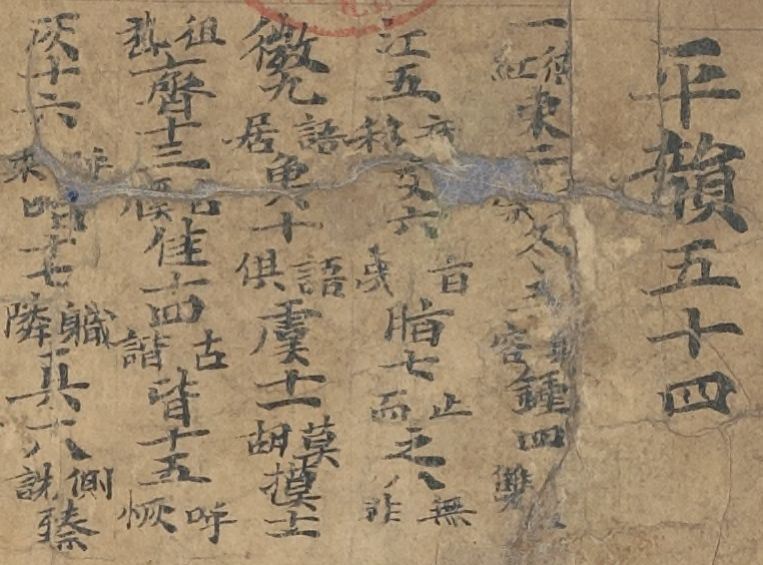
\includegraphics[width=0.90\textwidth]{Chapter5/fig12a P Chin 2017.jpg}
    \caption{Opening of the \emph{Qièyùn} from a Dūnhuáng fragment (PChin. 2017).}
    \label{fig:PChin}
\end{figure}


\begin{figure}[ht]
    \centering
%\begin{minipage}{0.4\columnwidth}
        \begin{tabular}{llll}
Transcription &  \multicolumn{3}{c}{Translation}
 \\
 {\large 平韻五十四}
 &
\multicolumn{3}{c}{There are 54 level tone rimes}
 \\
{\large 一}德紅{\large 東}

& 1. 東 tuwng 
& =
德 \textit{t(ok)}
& +
紅 \textit{(h)uwng} \\
{\large 二}都宗{\large 冬}

& 2. 冬 \textit{towng}
& =
都 \textit{t(u)}
& +
宗 \textit{(ts)owng} \\
{\large 三}職容{\large 鐘}

& 3. 鐘 \textit{tsyowng}
& =
職 \textit{tsy(ik)}
& +
容 \textit{(y)owng} \\
{\large 四}古雙{\large 江}

& 4. 江 \textit{kaewng}
& =
古 \textit{k(uX)}
& +
雙 \textit{(sr)aewng} \\
{\large 五}章移{\large 支}

& 5. 支 \textit{tsye}
& =
章 \textit{tsy(ang)}  
& +
移 \textit{(y)e} \\
{\large 六}旨夷{\large 脂}

& 6. 脂 \textit{tsyij} 
& =
旨 \textit{tsy(ijX)}
& +
夷 \textit{(y)ij} \\
{\large 七}止而{\large 之}

& 7. 之 \textit{tsyi}  
& =
止 \textit{tsy(iX)}
& +
而 \textit{(ny)i} \\
{\large 八}無非{\large 微}

& 8. 微 \textit{m{\sil{jɨj}}} 
& =
無 \textit{m(ju)}
& +
非 \textit{(p){\sil{jɨj}}} \\
{\large 九}語居{\large 魚}

& 9. 魚 \textit{ngjo}
& =
語 \textit{ng(joX)}
& +
居 \textit{(k)jo} \\
{\large 十}遇俱{\large 虞}

& 10. 虞 \textit{ngju}
& =
遇 \textit{ng(juH)}
& +
俱 \textit{(k)ju} \\
{\large 十一}莫胡{\large 模}

& 11. 模 \textit{mu}
& =
莫 \textit{m(aek)}
& +
胡 \textit{(h)u} \\
{\large 十二}徂嵇{\large 齊}

& 12. 齊 \textit{dzej}
& =
徂 \textit{dz(u)}
& +
嵇 \textit{(h)ej} \\
{\large 十三}古膎{\large 佳}

& 13. 佳 \textit{kea}
& =
古 \textit{k(uX)} 
& +
膎 \textit{(h)ea} \\
{\large 十四}古諧{\large 皆}

& 14. 皆 \textit{keaj}
& =
古 \textit{k(uX)}
& +
諧 \textit{(h)eaj} \\
{\large 十五}呼恢{\large 灰}

& 15. 灰 \textit{xwoj}
& =
呼 \textit{x(u)}
& +
恢 \textit{(kh)woj} \\
{\large 十六}呼來{\large 咍}

& 16. 咍 \textit{xoj}
& =
呼 \textit{x(u)}
& +
來 \textit{(l)oj} \\
{\large 十七}軄隣{\large 真}

& 17. 真 \textit{tsyin}
& =
軄 \textit{tsy(ik)}
& +
隣 \textit{(l)in} \\
{\large 十八}側詵{\large 臻}

& 18. 臻 \textit{tsrin}
& =
側 \textit{tsr(ik)}
& +
詵 \textit{(sr)in} \\
  ... &

 ... &
        \end{tabular}
%\end{minipage}
\caption{Transcription and translation of Figure \ref{fig:PChin}.}
\end{figure}


\paragraph{Rime categories of the
 \emph{Qièyùn}.} As already noted, the  \emph{Qièyùn}
classifies the readings of characters according to 193 different rime
categories. The  \emph{Qièyùn} itself makes no effort to meaningfully
group these rimes together into higher order categories or to elucidate
systematic relationships among them.\footnote{Once the phonetic value of
  the rimes has been made clear from other material it emerges that the
  order of rimes in the volumes belonging to different tones are
  parallel and phonetically motivated, e.g. within the \emph{píngshēng}
  rimes those that end with -n occur in a sequence and within the
   \emph{rùshēng} rimes those that end with -t occur in a sequence \citep[602]{Oh2017}. Later rime tables, beginning with the 13th century
  四聲等子  \emph{Sìshēng děngzǐ}, group together rimes into 摄
   \emph{shè}, a category roughly analogous to nuclear vowels \citep[133]{Coblin2006Zhang}.} Nonetheless, Baxter's transcription of Middle Chinese
rimes appears to reflect a language with the nuclear vowels -\emph{i}-,
-\emph{e}-, -\emph{ea}-, -\emph{ae}-, -\emph{{\sil{ɨ}}}-, -\emph{a}-,
-\emph{u}-, -\emph{o}- and the codas -\emph{ng}, -\emph{k}, -\emph{w},
-\emph{wng}, -\emph{wk}, -\emph{m}, -\emph{p}, -\emph{j}, -\emph{n},
-\emph{t}, -\emph{{\sil{ɨ}}}, but one must remember this system is not an
attempt at a phonetic or phonological rep­re­sen­ta­tion of Middle
Chinese but rather a transcription of all of the categories of the
 \emph{Qièyùn} (and the rime tables). Thus, the `\emph{jaep}' in the
transcription of a character 劫 as  \emph{kjaep} means that this
character appears under the  \emph{yè} 業 \emph{ngjaep} rime in the
 \emph{Qièyùn}.\footnote{As in the example just given, when reporting
  rime categories, I provide the pīnyīn reading of the character that
  names the category, the character itself, and its Middle Chinese
  reading, which is also an instance of the rime category in question.}
The entire inventory of 193 rime categories is here omitted as
unnecessary for the ensuing discussion.\footnote{Since the original
  edition of the  \emph{Qièyùn} is not extant research relies on later
  versions that offer different numbers of rime categories (\cite[74 et passim]{Chang1974}, \cite{Bottero2013}). For lists of the rime categories see
  \cite[74]{Chang1974},
  \cite[82-85]{Baxter1992}, 
  \cite[329-338]{Handel2009},
  \cite[17-20]{Baxter2014OldChinese}. The appendix (§) offers a look-up chart for Middle
  Chinese rimes on the basis of Baxter's transcription system. }

\paragraph{Initials categories of the
\emph{Qièyùn}.} Whereas rime categories are part of
the organization of the \emph{Qièyùn} as a document (i.e. they are
pre-defined as categories by their physical presentation), the work
reveals initial categories less straightforwardly. It would have been
convenient if the \emph{Qièyùn} only ever used one character to
represent a given initial in all \emph{fǎnqiè} spellings of character
readings that begin with that initial. Unfortunately, the \emph{Qièyùn}
is content to employ various \emph{fǎnqiè} spellers to indicate the same
initial. In order to distinguish which  \emph{fǎnqiè} spellers refer to
the same category, following a method elaborated by 陳澧 Chén Lǐ in his
切韻考 \emph{Qièyùn kǎo} of 1842, one links  \emph{fǎnqiè} onset spellers
(反切上字  \emph{fǎnqiè shǎngzì}) into chains by iteratively collecting
the \emph{fǎnqiè} onset speller used in the  \emph{fǎnqiè} spelling of
another \emph{fǎnqiè} onset speller. To pursue the English analogy, if
 \emph{f}(\emph{ake}) = \emph{f}(\emph{old}) +(\emph{c})\emph{ake},
 \emph{fold} =  \emph{ph}(\emph{one}) + (\emph{t})\emph{one}, and
 \emph{phone} = \emph{f}(\emph{ake}) + (\emph{sh})\emph{ield}, then
 \emph{fake},  \emph{fold}, and \emph{phone} all begin with the same
sound. To take a Chinese example, the following chain shows that
枯可苦康空楷口 and 客 all share the same onset.\footnote{Sometimes
  separate chains are linked by making use of the appearance of a
  character in two places in the \emph{Qièyùn}; this happens when a
  character has two different pronunciations. Both pronunciations are
  noted under both entries (with the notation 又音 \emph{yòuyīn }'also
  pronounced' applied to the alternative pronunciation). Thus, a
  character and its two pronunciations redundantly appear in two places
  in the body of the text. If the same pronunciation has two different
  \emph{fǎnqiè} initial spellers in its two locations these
  \emph{fǎnqiè} initial spellers can be used to link two chains that
  would otherwise remain broken (cf. 
  \cite[13-14]{Jacques2006Intro}).}

\begin{figure}[p]
    \centering
    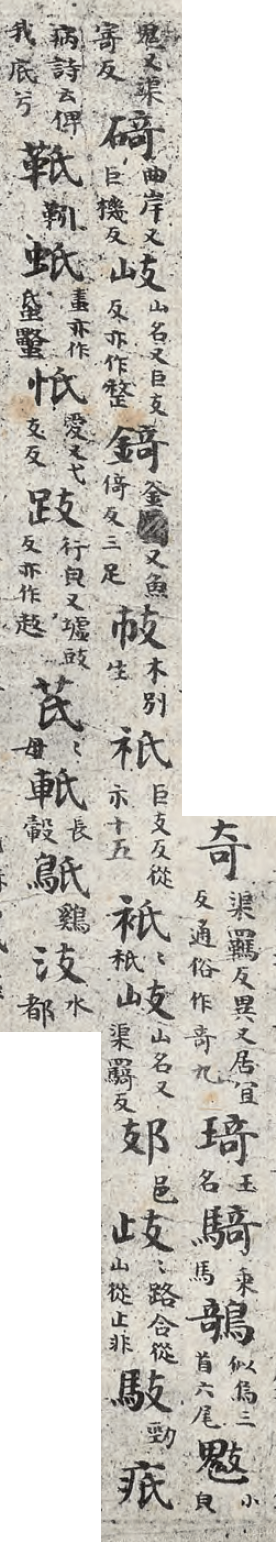
\includegraphics[height=1.46\textwidth]{Chapter5/gje.png}
    \caption{The homophone groups 奇 \textit{gje} and 祁 \textit{gjie} from the 刊謬補缺切韻 \textit{Kānmiù Bǔquē Qièyùn} of 706 CE.}
    \label{fig:Wang-gje-and-gjie}
\end{figure}

\begin{figure}[p]
\begin{adjustbox}{max width=1.3\textwidth,center}
    \centering
        \begin{tabular}{ll}
Transcription & Translation \\
\makecell[l]{{\large 奇}
渠羈反, \\ 異又居宜反,
通俗作奇九}
& \makecell[l]{1. {\large 奇 \textit{gje}} (渠 \textit{gjo} + 羈 \textit{kje} ), 異 also pronounced \textit{kje} (居 \textit{kjo} + 宜 \textit{ngje}), \\ 
 the vulgar writing is 竒. \\ A total of nine characters have the pronunciation gje.}
\\
{\large 琦}玉名
& 2. {\large 琦} name of a precious stone. \\
{\large 騎}乘馬
& 3. {\large 騎} ride a horse.  \\
{\large 鵸}似烏,三首六尾
& 4. {\large 鵸} like a crow, with three heads and six tails. \\
{\large 鬾}小兒鬼又渠寄反
& 5. {\large 鬾} ghost of a small child; also pronounced 渠 \textit{gjo} + 寄 \\
{\large 碕}曲岸又巨機反
& 6. {\large 碕} curved shore, also pronounced \textit{g{\sil{jɨj}}} (巨 \textit{gjoX} + 機 \textit{{\sil{kjɨj}}}). \\
{\large 岐}山名又巨支反亦作
& \makecell[l]{7. 岐 name of a mountain; also pronounced \textit{gje} (巨gjoX+支tsye); \\ also written .} \\
{\large 錡}釜屬又魚倚反三足 
& 8. {\large 錡} a type of cauldron; also pronounced ngjeX (魚 ngjo+倚 'jeX), with three legs.\\
{\large ��}木別生
& 9. {\large ��} [something] growing separately [from] a tree', [i.e. an arboreal parasite.] \\
& \\
{\large 祁}巨支反從示十五
& \makecell[l]{1. {\large 祁} \textit{gjie} (巨 \textit{gjoX} + 支 \textit{tsye}), from 示 'spirit'. \\ A total of fifteen characters have the pronunciation \textit{gjie}.} \\
{\large 衹}〻秖
& 2. {\large 衹} The first syllable of 衹秖 'monastic robes'. \\
{\large 岐}山名又渠羈反
& 3. {\large 岐} name of a mountain; also pronounced \textit{gje} (渠 \textit{gjo} + 羈 \textit{kje}). \\
{\large ��}邑
& 4. {\large ��} town (邑).\\
{\large 歧}〻路合從山從止非
& 5. {\large 歧} crossroad. From 山 not from 止. \\
{\large 馶}勁
& 6. {\large 馶} strong (勁). \\
{\large 疧}病《詩》云「俾我底兮」 
& 7. {\large 疧} sick; the Odes say 俾我底兮 'makes me sick!' \\
{\large ��}靷
& 8. {\large ��} leather belt that connects a horse with a cart (靷). \\
{\large 蚔}䖯亦作��
& 9. {\large 蚔} poisonous insect (䖯), also written �� and. \\
{\large 忯}愛又弋支反
& 10. 忯 love; also pronounced \textit{ye}  (弋 \textit{yik} + 支 \textit{tsye}) \\
{\large 跂}行兒又墟豉反亦作䞚
& \makecell[l]{11. 跂 walk like a child (i.e. crawl); also pronounced \textit{khje} (墟 \textit{khjo} +豉 \textit{dzye}), \\ also written 䞚.} \\
{\large 芪}〻母
& 12. {\large 芪} first syllable of 芪母, a kind of medicinal grass. \\
{\large 軝}長轂
& 13. {\large 軝} protruding part of a hub (長轂). \\
{\large 䲬}鷄
& 14. {\large 䲬} chicken (鷄). \\
{\large 汥}水都
& 15. {\large 汥} aggregation of water.
        \end{tabular}
\end{adjustbox}
\caption{The homophone groups 奇 \textit{gje} and 祁 \textit{gjie} from the 刊謬補缺切韻 \textit{Kānmiù Bǔquē Qièyùn} of 706 CE. (A transcription and translation of \ref{fig:Wang-gje-and-gjie})}
\end{figure}


\begin{description} \item
可 \emph{khaX} = 枯 \emph{kh}(\emph{u})+ 我 (\emph{ng})\emph{aX}
\item
枯  \emph{khu} = 苦  \emph{kh}(\emph{uX})+ 胡 (\emph{h})\emph{u}
\item
苦  \emph{khuX} = 康  \emph{kh}(\emph{ang}) + 杜 (\emph{d})\emph{uX}
\item
康 \emph{khang} = 苦  \emph{kh}(\emph{uX}) + 岡 (\emph{k})\emph{ang}
\item
空 \emph{khuwng} = 苦  \emph{kh}(\emph{uX}) + 紅 (\emph{h})\emph{uwng}
\item
楷  \emph{khojX} = 苦  \emph{kh}(\emph{uX}) + 駭 (\emph{h})\emph{ojX}
\item
口 \emph{kuwX} = 苦  \emph{kh}(\emph{uX}) + 後 (\emph{h})\emph{uwX}
\item
客 \emph{khæk} = 苦 \emph{kh}(\emph{uX}) + 格 (\emph{k})\emph{æk}
\end{description}


The result of applying this method to all  \emph{fǎnqiè} onset spellers
in the \emph{Qièyùn} is 51 chains of  \emph{fǎnqiè} onset spellers (聲類
 \emph{shēnglèi}). These onset classes are not phonemes, but merely
chains of onset \emph{fǎnqiè} spellers assembled philologically. The
 \emph{Qièyùn} is silent on the phonetic value of these 51 onset classes.
For their phonetic value we turn to the rime tables.

The  \emph{Yùnjìng} explicitly distinguishes initials into place and
manner of articulation with terms such as labial (唇 \emph{chún}),
dental (舌 \emph{shé}), voiceless (清 \emph{qīng}), voiceless aspirated
(次清 \emph{cìqīng}), etc. the \emph{Qīyīnlüè} distinguishes 36 initials
by giving an example of each.\footnote{The preface to the  \emph{Yùnjìng}
  contains a list of the same list of 36 initials, but the body of the
  text does not classify characters according to these initials.} Thus,
what the  \emph{Yùnjìng} describes as a `voiceless labial' the
 \emph{Qīyīnlüè} refers to acrophonically as the 幫 \emph{p}(\emph{ang})
initial. Whereas associating sounds with the 51 onsets of the
 \emph{Qièyùn} on the basis of internal evidence is not possible,
associating sounds with the 36 initials of the \emph{Qīyīnlüè} and the
articulatory categories of the \emph{Yùnjìng} is feasible. Hereafter I
refer to `the rime tables' when the distinction between the
 \emph{Yùnjìng} and the the \emph{Qīyīnlüè} is clear or unimportant.

Some effort must be taken to reconcile the 36 rime table initials of
relatively known phonetic interpretation with the  \emph{Qièyùn}'s 51
onsets of unknown phonetic value. There are cases where the rime tables
split cat­e­gories which can be linked in the  \emph{Qièyùn} and cases
where the rime tables conflate categories which cannot be linked in the
 \emph{Qièyùn} (\cite[45-61]{Baxter1992}, 
 \cite[14-16]{Baxter2014OldChinese}). The
splits reflect conditioned changes in the pronunciation of Chinese
during the centuries intervening the composition of the the works in
question and need concern us no further here.\footnote{The 9th century
  Buddhist monk 守溫 Shǒuwēn is traditionally credited with enumerating
  the 36 initials, but fragments from 敦煌 Dūnhuáng potentially
  creditable to him enumerate only 30 initials (\cite[206-207]{Pulleyblank1970LateMC}, 
  \cite{Coblin2006reflections}). The 30 initials omit some of the subsequent
  innovations. In particular, the the labiodental fricatives
  (\emph{qīngchún} 輕唇), viz. 非 f-, 敷 fh, 奉 v-, 微 ɱ- of the later
  36-initials \citep[41, 46-47]{Baxter1992}
  are not listed in the 30
  initials, although the fragment may show an awareness of their
  distinct pronunciation (\cite[210]{Pulleyblank1970LateMC}, 
  \cite[118]{Coblin2006reflections}). }
The latter cases, in which the rime tables collapse categories distinct
in the \emph{Qièyùn}, are of interest because the rime tables may
correctly subsume under one initial category  \emph{fǎnqiè} onset chains
that are in com­ple­men­tary distribution with respect to \emph{Qièyùn}
rime categories. Let us consider two examples \citep[112-114]{Tang2002}. 

In the first example the rime tables categorize some characters as
having the 照母 \emph{zhàomǔ} initial (here provisionally written
 \emph{č}-) which the \emph{Qièyùn} puts in the distinct \emph{fǎnqiè}
chains 側莊阻鄒簪仄爭 and 之職章諸旨止脂征正占支煮 (here provisionally
distinguished as \emph{č{\sil{₁}}- } and \emph{č{\sil{₂}}- } respectively); see . The
initials \emph{č{\sil{₁}}}- and \emph{č{\sil{₂}}}- must be considered distinct because
there are some rime categories com­patible with both, in particular
-\emph{ik} (\emph{zhí~}職 \emph{~tsyik}), -\emph{jang
}(\emph{yáng~}陽 \emph{~yang}), and -\emph{jo
}(\emph{yú~}魚 \emph{~ngjo}), i.e.  \emph{č{\sil{₁}}}- and \emph{č{\sil{₂}}}- are not in
com­ple­men­tary distribution with respect to the  \emph{Qièyùn} rime
categories. Thus, in his transcription system Baxter distinguishes
 \emph{tsr}- (pro­vi­sional \emph{č{\sil{₁}}}-) and \emph{tsy}- (provisional
 \emph{č{\sil{₂}}}-).


\begin{figure}[t]
\centering
\begin{minipage}[c]{\textwidth}
\centering
        \begin{tabular}{lllll}
\multicolumn{2}{l}{fǎnqiè onset speller (its rime)}
 &&
\multicolumn{2}{l}{fǎnqiè onset speller (its rime)} \\
側 \textit{č{\sil{₁}}ik} &
(\textit{zhí} 職 \textit{tsyik}) &&

之 \textit{č{\sil{₂}}i } &
(\textit{zhī} 之 \textit{tsyi}) \\
莊 \textit{č{\sil{₁}}jang} & 
(\textit{yáng} 陽 \textit{yang})\footnote{The reading of the character 莊 č{\sil{₁}}jang is described as an initial voiceless affricate (齒音 chǐyīn, 清 qīng) on chart 31 of the Yùnjìng and as initial č- (照 zhào) on chart 34 of the Qīyīnlüè. \\
}
&&

職 \textit{č{\sil{₂}}ik} &
(\textit{zhí} 職 \textit{tsyik}) \\
阻 \textit{č{\sil{₁}}joX} &
(\textit{yú} 魚 \textit{ngjo})&&

章 \textit{č{\sil{₂}}jang} &
(\textit{yáng} 陽 \textit{yang}) \\
鄒 \textit{č{\sil{₁}}juw} &
(\textit{yóu} 尤 \textit{hjuw}) &&

諸 \textit{č{\sil{₂}}jo} &
(\textit{yú} 魚 \textit{ngjo}) \\
簪 \textit{č{\sil{₁}}im} &
(\textit{qīn} 侵 \textit{tshim}) &&

旨 \textit{č{\sil{₂}}ijX} &
(\textit{zhī} 脂 \textit{tsyij}) \\
仄 č{\sil{₁}}ik  &
(\textit{zhí} 職 \textit{tsyik}) &&

止 \textit{č{\sil{₂}}iX} &
(\textit{zhī} 之 \textit{tsyi})\footnote{The reading of the character 止 č{\sil{₂}}iX is described as an initial voiceless affricate (齒音 shéchǐ, 清 qīngzhuó) on chart 8 of the Yùnjìng and as č- (照 zhào) on chart 8 of the Qīyīnlüè.}
\\
爭 \textit{č{\sil{₁}}eang}  &
(\textit{gēng} 耕 \textit{keang}) &&

脂 \textit{č{\sil{₂}}ij}  &
(\textit{zhī} 脂 \textit{tsyij}) \\

&&&

征 \textit{č{\sil{₂}}eng}  &
(\textit{qīng} 清 \textit{tshjeng}) \\

&&&

正 \textit{č{\sil{₂}}eng} &
 (\textit{qīng} 清 \textit{tshjeng}) \\

&&&

占 \textit{č{\sil{₂}}em}  &
(\textit{yán} 鹽 \textit{yem}) \\

&&&

支 \textit{č{\sil{₂}}e}  &
(\textit{zhī} 支 \textit{tsye}) \\

&&&

煮 \textit{č{\sil{₂}}joX}  &
(\textit{yú} 魚 \textit{ngjo})\\
\end{tabular}        \caption{The fǎnqiè onset speller chains  č{\sil{₁}}- and č{\sil{₂}}-, 
distinguishable in the \textit{Qièyùn} but not in the rime tables}
    \label{fig:fanqiec1c2}
\end{minipage}
\end{figure}

In the second example the rime tables categorize characters as having
the 來母 \emph{láimǔ} initial (here provisionally written \emph{l}-)
which the \emph{Qièyùn} puts in the distinct  \emph{fǎnqiè} chains
盧郎落魯來洛勒賴練 and 力良呂里林離連縷 (here provisionally
distinguished as \emph{l{\sil{₁}}- }and \emph{l{\sil{₂}}- }respectively); see . In this
case there are no rimes that occur in both  \emph{fǎnqiè} onset chains.
Thus, the rimes themselves sufficiently index the two types of
 \emph{l}-. The two are in complementary distribution and may be
re­gard­ed as allophones of the same phoneme (perhaps a `light l' and a
'dark l'). Because of their complementary distribution, Baxter's
transcription uses \emph{l}- for the Middle Chinese pro­nun­ci­a­tions
of characters written with both \emph{fǎnqiè} chains.\footnote{I have
  taken a methodologically unwarranted short cut. What I show here is
  that the rhymes of the initial \emph{fǎnqiè} spellers themselves are
  in complementary distribution, but better would be to show that all of
  the rimes in which words spelled with these spellers occur are in
  complementary distribution.}

By testing in this way all pairs of  \emph{fǎnqiè} onset chains in the
 \emph{Qièyùn} that are not assigned by the rime tables to distinct
initials, as to whether or not the two chains are in complementary
distribution relative to \emph{Qièyùn} rime categories, one reduces the
51 distinct  \emph{fǎnqiè} onset chains to 42 distinct  \emph{Qièyùn}
initials (聲母~ \emph{shēngmǔ}), as presented in .\footnote{The terms in
  are not necessarily those of any particular primary source, but
  instead are traditional in the teaching of Middle Chinese phonology.
  Although there is no traditional Chinese name for initial  \emph{zr}-,
  I herein refer to it as 俟  \emph{sì}
  \citep[15-46]{Baxter2014OldChinese}.}

The reader may protest that by observing the patterns of distribution
between the 51  \emph{fǎnqiè} onset chains in the  \emph{Qièyùn} and the
193 rime categories of the  \emph{Qièyùn}, one could establish without
reference to the rime tables that the  \emph{fǎnqiè} onset chain of which
盧 \emph{lú} is a member and that of which 力~ \emph{lì }is a member can
be united, whereas the chains of which 側 \emph{cè }and 之 \emph{zhī}
are respectively members cannot be. This al­ter­na­tive method, reducing
the 51  \emph{fǎnqiè} onset chains to a smaller number of distinct
initial cate­gories while ignoring the rime tables avoids the
anachronism of using a book from 1161 to analyze the categories of a
book from 601. Nonetheless, the alternative method has the practical
disadvantage of arriving at a number of initials lower than 42 which
the entire edifice of historical Chinese linguistics operates with.
Although conceptually this is an advantage, since it demonstrates that
the the rime tables distort one's perception of the  \emph{Qièyùn}, and
one may express the hope that in the future the 42 initials will be
abandoned as the dross of tradition, to propose an alternative analysis
here would take us well beyond the scope of this work's intended scope
and potentially confuse the student uniformly finds 42 initials
discussed in other works. To give an example, initials 泥 \emph{n}- and
娘 \emph{nr}-, although in com­ple­men­tary distribution, are usually
regarded as distinct Middle Chinese initials because they are
dis­tin­guished in the rime tables .\footnote{Note that 30
  initials of the Dūnhuáng fragments (see note ) omit initial 娘
  \emph{nr-}. Initials 匣 \emph{h-} and 雲 \emph{hj-} (the latter a
  subset of the 喻 yù initial category of the rime tables) are
  also in complementary distribution.}

The true drawback of ignoring the rime tables is that one then loses the
phonetic information that the two  \emph{fǎnqiè} onset chains which 盧
 \emph{lú} and 力 \emph{lì} respectively belong to are classed in the
rime tables as having an initial liquid resonant (舌齒 \emph{shéchǐ},
清濁 \emph{qīngzhuó}) or lateral (來目  \emph{láimù}) and that the two
chains which 側 \emph{cè} and 之 \emph{zhī} respectively belong to are
classed in the rime tables as having an initial voiceless affricate
(齒音 \emph{shéchǐ}, 清 \emph{qīngzhuó}) or 照母  \emph{zhàomǔ} initial.

\begin{figure}[t]
\centering
\begin{minipage}[c]{\textwidth}
\centering
        \begin{tabular}{lllll}
\multicolumn{2}{l}{fǎnqiè onset speller (its rime)}
 &&
\multicolumn{2}{l}{fǎnqiè onset speller (its rime)} \\
盧 \textit{l{\sil{₁}}u} & (\textit{mó} 模 \textit{mu}) &&
力 \textit{l{\sil{₂}}ik} & (\textit{zhí}  職 \textit{tsyik}) \\
郎 \textit{l{\sil{₁}}ang} &
(\textit{táng} 唐 \textit{dang}) && 
良 \textit{l{\sil{₂}}jang} &
(\textit{yáng} 陽 \textit{yang}) \\

落 \textit{l{\sil{₁}}ak} &
(\textit{duó} 鐸 \textit{dak}) &&

呂 \textit{l{\sil{₂}}joX} & 
(\textit{yú} 魚 \textit{ngjo}) \\

魯 \textit{l{\sil{₁}}uX}  &
(\textit{mó} 模 \textit{mu}) &&

里 \textit{l{\sil{₂}}iX} &
(\textit{zhī} 之 \textit{tsyi}) \\

來 \textit{l{\sil{₁}}oj} &
(\textit{hāi} 咍 \textit{xoj}) &&

林 \textit{l{\sil{₂}}im} &
(\textit{qīn} 侵 \textit{tshim}) \\

洛 \textit{l{\sil{₁}}ak} &
(\textit{duó} 鐸 \textit{dak}) &&

離 \textit{l{\sil{₂}}je} &
(\textit{qí} 齊 \textit{tsij}) \\


勒 \textit{l{\sil{₁}}ok}  &
(\textit{dé} 德 \textit{tok}) &&

連 \textit{l{\sil{₂}}jen} &
(\textit{xiān} 仙 \textit{sjen})\footnote{The reading of the character 連 \textit{l{\sil{₂}}jen} (\textit{xiān} 仙 \textit{sjen}) is described as a initial liquid resonant (舌齒 \textit{shéchǐ}, 清濁 \textit{qīngzhuó}) on chart 23 of the \textit{Yùnjìng} (Figure 17) and as l- (來 \textit{lái}) on chart 23 of the \textit{Qīyīnlüè} (Figure 18).} \\

賴 \textit{l{\sil{₁}}ajH} &
(\textit{tài} 泰 \textit{thajH}) &&

縷\textit{ l{\sil{₂}}juX} &
(\textit{yú} 虞 \textit{ngju}) \\

練 \textit{l{\sil{₁}}enH} &
(\textit{xiān} 先 \textit{sen})\footnote{The reading of the character 練 \textit{l{\sil{₁}}enH} is described as a initial liquid resonant (舌齒 \textit{shéchǐ}, 清濁 \textit{qīngzhuó}) on chart 23 of the \textit{Yùnjìng} (Figure 17) and as l- (來 \textit{lái}) on chart 23 of the \textit{Qīyīnlüè} (Figure 18).} &&& 

\end{tabular}        \caption{The fǎnqiè onset speller chains  \textit{l{\sil{₁}}}- and \textit{l{\sil{₂}}}-,  distinguishable in the Qièyùn but not in the rime tables}
    \label{fig:fanqiel1l2}
\end{minipage}
\end{figure}

\paragraph{The `ranks' of the rime tables and
`divisions' of the
 \emph{Qièyùn}.} Without explanation the rime tables
classify rimes among four 等~ \emph{děng} `ranks'. These `ranks' refer
fundamentally to the \emph{mise-en-page} of these two particular
documents, each rank corresponding to a row on a page. Although the
linguistic meaning of these `ranks' is obscure, they bear certain
relationships with dis­tri­bu­tional classes of co-occurrences between
initials and rimes in the \emph{Qièyùn} (\cite[7]{Schuessler2009minimal}, 
\cite[]{Shen2017}). In English it is useful to distinguish between `rank' as
the term for the four rows of the rime tables and `division' for the
analogous but distinct categories in the  \emph{Qièyùn}, even though the
Chinese term 等~ \emph{děng} is the same in both cases 
\citep[13]{Shen2017}. The paraphrase of `ranks' into `divisions' proceeds in two
steps. Jiāng Yǒng 江永 (1681-1762) took the first step in his 四聲切韻表
 \emph{Sìshēng Qièyùnbiǎo}; he looked up characters in each \emph{Qièyùn
}rime category to see which `rank' the rime tables place them in. Using
this procedure the rime categories of the  \emph{Qièyùn} divide into four
classes: (1) rimes that contain characters appearing in rank-i only, (2)
rimes that contain characters appearing in rank-ii only, (3) rimes that
contain mostly characters that appear in rank-iii, but containing some
characters appearing in rank-ii or rank-iv, (4) rimes that contain only
characters put into rank-iv (Shen Ruiqing 2017: 16). These classes of
rimes we may respectively dub `division-i rimes', `division-ii rimes',
'division-iii rimes', and `division-iv rimes'.\footnote{One explanation
  for the appearance of division-iii rimes in rank-ii is the sound
  change \emph{Tsrj}- \textgreater{} \emph{Tsr}- (cf. 
  \cite[267-269, 580-581]{Baxter1992}.} These `divisions' are hybrid beasts, with the rime
categories of the  \emph{Qièyùn} and the ranks of the rime tables as
their parents. In the second step, the realization that the divisions so
defined mostly coincide with dis­tri­bu­tional classes of  \emph{Qièyùn}
initials allows one to redefine the divisions using these co-occurence
patterns, and thereby avoid referring to rime table ranks. Rimes of all
four divisions occur with laryngeal (\emph{hóu} 喉 \emph{H}-), velar
(\emph{yá} 牙 \emph{K}-), and labial initials (\emph{chún }唇
 \emph{P}-). Retroflex stops (\emph{shéshǎng} 舌上 \emph{Tr}-) and
retroflex sibilants (\emph{zhuāngzǔ} 莊組  \emph{Tsr}-) initials occur
only with division-ii rimes; initial 來 \emph{l}- does not occur with
division-ii rimes. Palatal initials (\emph{zhāngzǔ} 章組 \emph{Tsy}-)
occur only with division-iii rimes.\footnote{If these co-occurrence
  patterns were articulated in terms of distinct  \emph{fǎnqiè} onset
  chains (聲類 \emph{shēnglèi}) instead of with initials
  (聲母~ \emph{shēngmǔ}), one could further observe that \emph{l{\sil{₂}}}- only
  occurs with division-iii rimes.} Dental initials (\emph{shétóu} 舌頭
 \emph{T}-) occur only with division-i and division-iv rimes. In fact,
rimes of division-i and division-iv pattern identically with regard to
their co-occurence with initials.\footnote{Most Chinese dialects show a
  prevocalic glide in division-iv words, e.g. 牽 Mandarin \emph{qiān}
  \textless{} MChi. \emph{khen. }The presence of this medial is
  presumably the reason the rime tables place these words in division-iv
  rather than division-i. Baxter argues that this medial arose due to a
  sound change affecting inherited front vowels between the composition
  of the  \emph{Qièyùn} and the composition of the rime tables 
  \citeyearpar[241-243]{Baxter1992}.} Thus, from the perspective of the  \emph{Qièyùn} it is
impossible to distinguish between division-i and division-iv; they can
be treated as a single division-i/iv (see ).

These statements of attested co-occurrence between a class of rimes and
a class of initials may be understood as the defining criteria of the
three divisions (viz. i/iv, ii, and iii) based on the internal evidence
of the \emph{Qièyùn.} In other words, the unsatisfactory
characterization of the ranks as an idiosyncrasy of the page formatting
of the rime tables is thus paraphrasable as linguistically meaningful
dis­tri­bu­tional classes in the  \emph{Qièyùn}.

\begin{figure}
    \centering
\begin{tabular}{|lr|l|l|l|l|l|l|l|}
\hline
唇音 & P- &  
幫 \textit{p-} &
滂 \textit{ph-} &
並 \textit{b-} &
明 \textit{m-} &&&
\\ \hline
舌頭音 & T- &
端 \textit{t-} &
透 \textit{th-} &
定 \textit{d-} &
泥 \textit{n-} &&&
\\ \hline
舌上音 & Tr- &
知 \textit{tr-} &
徹 \textit{trh-} &
澄 \textit{dr-} &
娘 \textit{nr-} &&&
\\ \hline
齒頭音 & Ts- &
精 \textit{ts-} &
清 \textit{tsh-} &
從 \textit{dz-} &
&
心 \textit{s-} &
邪 \textit{z-} &
\\ \hline
莊組 & Tsr- &
莊 \textit{tsr-} &
初 \textit{tsrh-} &
崇 \textit{dzr-} &
&
生 \textit{sr-} &
俟 \textit{zr-} &
\\ \hline
章組 & Tsy- &
章 \textit{tsy-} &
昌 \textit{tsyh-} &
禪 \textit{dzy-} &
日 \textit{ny-} &
書 \textit{sy-} &
船 \textit{zy-} &
以 \textit{y-} \\ \hline
牙音 & K- &
見 \textit{k-} &
溪 \textit{kh-} &
群 \textit{g-} &
疑 \textit{ng-} &
&& \\ \hline


喉音 &&
影 \textit{'-} &
曉 \textit{x-} &
匣 \textit{h-} &
&&&
云 \textit{hj-}
\\ \hline
半舌音 &&
來 \textit{l-} &&&&&& \\
\hline
\end{tabular}
    \caption{The 42 initials of the Qièyùn 
    \citep[15]{Baxter2014OldChinese}}
    \label{fig:34-initials}
\end{figure}

\begin{figure}
    \centering
    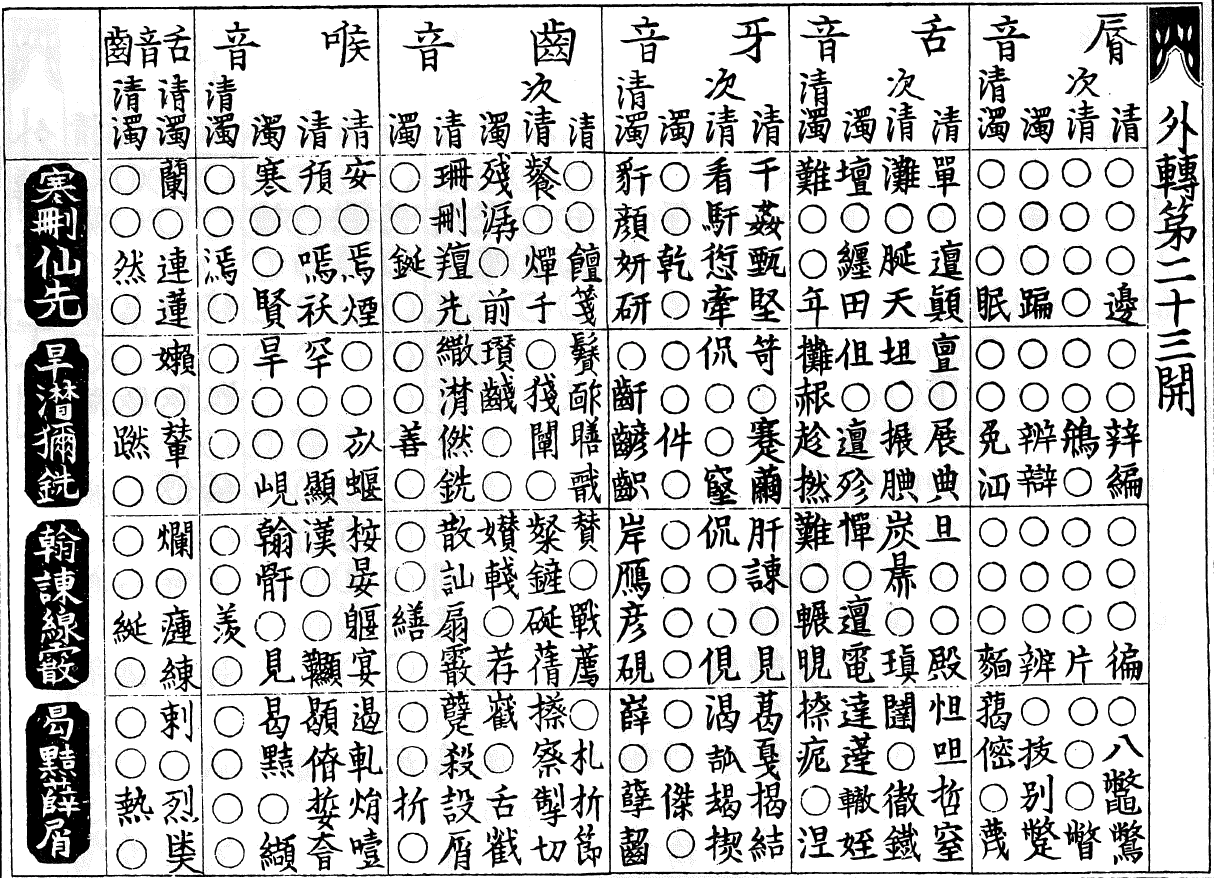
\includegraphics[width=1\textwidth]{Chapter5/fig17 Yunjing 23 version 1.png}
    \caption{Chart 23 from the \textit{Yùnjìng}}
    \label{fig:Yunjing23}
\end{figure}

A more thoroughgoing presentation of the co-occurrence restrictions of
the initial classes with rimes further permits division-i/iv and
division-ii to be collapsed. Division-i/iv rimes occur with dental
(\emph{shétóu} 舌頭 \emph{T}-) and affricate initials (\emph{chǐtóu}
齒頭 \emph{Ts}-) but not with retroflex (\emph{shéshǎng} 舌上
 \emph{Tr}-) or retroflex affricate (\emph{zhuāngzǔ} 莊組 \emph{Tsr}-)
initials. Division-ii occurs with retroflex (\emph{shéshǎng} 舌上
 \emph{Tr}-) and retroflex affricates (\emph{zhuāngzǔ}~莊組 \emph{Tsr}-)
but not with dental (\emph{shétóu} 舌頭  \emph{T}-) or affricate
(\emph{chǐtóu} 齒頭~ \emph{Ts}-) initials. Thus, division-i/iv is in
com­ple­men­tary distribution with division-ii; those places where the
one is allowed the other is forbidden, although both are forbidden from
the palatals (\emph{zhāngzǔ} 章組  \emph{Tsy}-). This com­ple­men­tary
distribution permits division-i/iv and division-ii to be united. From
this new perspective division-i/iv/ii bears the name `type A' and
division-iii bears the name `type B' (see ). The dis­tri­bu­tional
categories of the  \emph{Qièyùn} itself permit analysis either in terms
of the three division-i/iv, division-ii, and division-iii or of the two
types A and B. Whether one speaks of divisions or types is simply a
question of which dis­tri­bu­tional facts are in focus. Both ways of
looking at the co-occurence of initial categories with rime categories
are syn­chron­i­cally true of Middle Chinese as reflected in the
 \emph{Qièyùn}. Nonetheless, in practice the terminology of `divisions'
in used with reference to Middle Chinese and the terminology of `types'
is used with reference to Old Chinese.

\begin{figure}
    \centering
    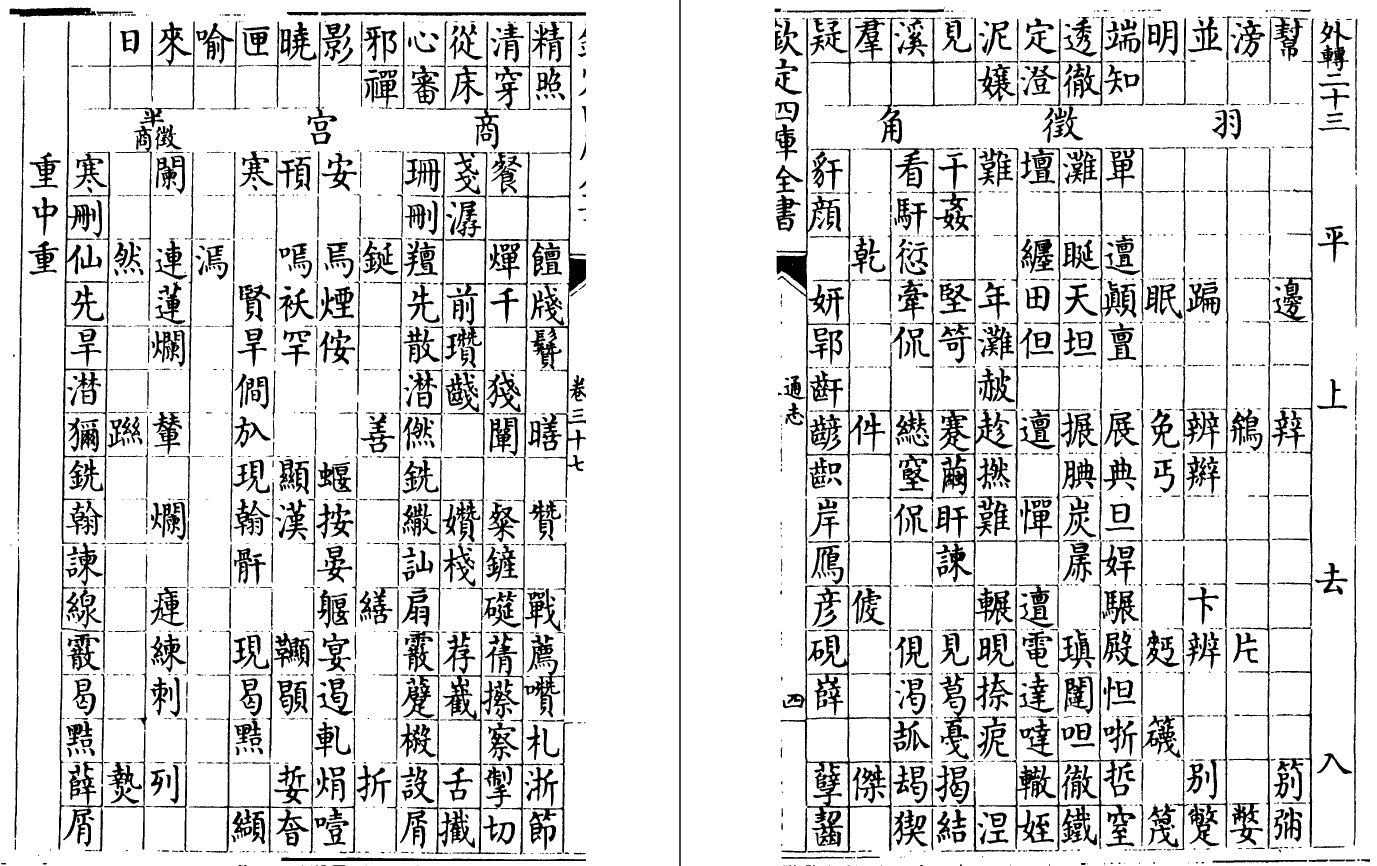
\includegraphics[width=1\textwidth]{Chapter5/fig18 Qiyinlue 23 version 1.png}
    \caption{Chart 23 from the \textit{Qīyīnlüè}}
    \label{fig:Qinyinlue23}
\end{figure}


In Baxter's Middle Chinese notation division-ii rimes are marked with
the vowels -\emph{ea}- and -\emph{ae}- and division-iii rimes are marked
with a main vowel -i- or pre-vocalic -j- (orthographically omitted after
initial palatals, i.e.  \emph{zhāngzǔ} 章組  \emph{Tsy}-) 
\citep[67-75]{Baxter1992}.\footnote{Note that in Baxter's system -\emph{ea}- occurs only in
  division-ii whereas -\emph{ae}- occurs in both division-ii and
  division-iii, so it is only in the absence of -\emph{j}- or -\emph{y}-
  in the onset that -\emph{ae}- by itself indexes division-ii.} The lack
of an indication of division-ii or division-iii using these conventions
itself indexes syllables of division-i/iv in Baxter's system; among
these syllables division-iv are indicated with the nuclear vowel
-\emph{e}-, whereas division-i syllables occur with -\emph{a}-,
-\emph{u}-, or -\emph{o}-. Following a suggestion of
\citet[]{Norman1994},
Baxter \& Sagart posit pharyn­geal­iza­tion in Old Chinese as the origin
of type A syllables and non-pharyngealization as the origin of type B
syllables 
\citeyearpar[68-76]{Baxter2014OldChinese}. For the present purposes this hypothesis can be
viewed as a mechanical rewriting of Middle Chinese syllables without -j-
as Old Chinese syllables with -{\sil{ˤ}}- (not applied to syllables with the
main vowel -i-) and the concomitant omission of -j- in the Old Chinese
ancestors of Middle Chinese words that contain -j-.\footnote{To the
  extent that one relies on late sources such as the  \emph{Guǎngyùn},
  the post-\emph{Qièyùn} sound change *TSrj \textgreater{} TSr-
  complicates this otherwise mechanical rewriting
  \citep[53-54]{Baxter1992}.}

\begin{figure}
    \centering
\begin{tabular}{|l|l|l|l|l|l|l|}
\hline
     &  l- & T- & Tr- & Ts- & Tsy- & Tsr- \\
\hline
Division-i & {\sil{✓}} & {\sil{✓}} && {\sil{✓}} && \\
\hline
Division-ii & & & {\sil{✓}} & & & {\sil{✓}} \\
\hline
Division-iii & {\sil{✓}} && {\sil{✓}} && {\sil{✓}} & {\sil{✓}} \\
\hline
Division-iv & {\sil{✓}} & {\sil{✓}} && {\sil{✓}} && \\
\hline
\end{tabular}
    \caption{Co-occurrence of rimes of the four divisions with various types of Middle Chinese initials}
    \label{fig:co-occurence-of-divisions}
\end{figure}

\begin{figure}
    \centering
\begin{tabular}{|l|l|l|l|l|l|l|}
\hline
     &  l- & T- & Tr- & Ts- & Tsy- & Tsr- \\
\hline
Type-A & {\sil{✓}} & {\sil{✓}} & {\sil{✓}} & {\sil{✓}} && {\sil{✓}} \\
\hline
Type-B & {\sil{✓}} & & {\sil{✓}} & & {\sil{✓}} &  {\sil{✓}} \\
\hline
\end{tabular}
    \caption{Co-occurrence of the rimes of type A and B with various types of Middle Chinese initials}
    \label{fig:co-occurence-of-A-and-B}
\end{figure}


\paragraph{Medial -\emph{w}- (合口
 \emph{hékŏu}) according to the rime tables.}
The presence or absence of a medial -\emph{w}- in Middle Chinese is of
significance for the reconstruction of Old Chinese. Reference to the
 \emph{Qièyùn} alone does not allow for the identification of this
distinction. The rime tables make the distinction explicit. A given
table of the  \emph{Yùnjìng} (but not of the  \emph{Qīyīnlüè}) is labelled
on its far right as either entirely 合口  \emph{hékŏu} `closed mouth' or
開口 \emph{kāikŏu} `open mouth'.\footnote{In fact, the situation is more
  complex. First, some tables are labeled 開合  \emph{kāihé}. Second,
  modern textbooks more or less tacitly `correct' the primary sources.
  For example, 中 is treated as 合口  \emph{hékǒu} in textbooks, although
  it appears on chart 1 of  \emph{Yùnjìng}, which is labeled 開
   \emph{kāi}. Such discrepancies, seldom discussed explicitly, are in
  need of systematic and methodologically informed study. I thank Zev
  Handel for his help with this note and this entire chapter.} As these
terms themselves suggest, all re­searchers analyze the syllables
categorized under these rubrics as respectively with -\emph{w}- and
without -\emph{w}- (e.g, 
\cite[62]{Baxter1992},
\cite[9]{Schuessler2009minimal},
\cite[2013-204]{Baxter2014OldChinese}).

The \emph{hékŏu }versus \emph{kāikŏu} distinction is not contrastive
after labial initials, as revealed by the inconsistent placement of
labial initial words in the rime tables and inconsistent use of
 \emph{fǎnqiè} rime spellers (反切下字  \emph{fǎnqiè xiàzì}) with these
words in the \emph{Qièyùn}
\citep[62-63]{Baxter1992}.

\paragraph{The 重紐 \emph{chóngniǔ} problem.} Historical Chinese phonologists in the tradition of Karlgren
(1964{[}1957]) fill out the categories of the  \emph{Qièyùn} and rime
tables with phonetically meaningful alphabetic representations. In most
cases---rimes, initials,  \emph{hékŏu}/ \emph{kāikŏu}---the phonetic
terminology of the rime tables or a look at Chinese dialects immediately
suggests a phonetic interpretation of the philological category in
question. However, in one case, the so-called 重紐 `\emph{chóngniǔ}
problem', a distinction present in the  \emph{Qièyùn} resisted
confirmation and analysis for a long time.

As with other niceties of Middle Chinese phonology, the  \emph{chóngniǔ}
problem boils down to an observation about the  \emph{mise-en-page} of
the  \emph{Qièyùn} and the rime tables. The term `\emph{chóngniǔ'} means
'repeated button', where `button' refers to the dot that separates
homophone groups within the same rime category in the presentation of
rime books deriving from the  \emph{Qièyùn}. The extant fragments
indicate that the original edition of the  \emph{Qièyùn} did not use this
device 
\citep[36]{Bottero2013}. In the preface to the earliest complete
version, namely 王仁昫 Wáng Rénxù's 刊謬補缺切韻 \emph{Kānmiù Bǔquē
Qièyùn} of 706 CE, the author says that he will separate homophone
groups with red dots 
\citep[41]{Bottero2013}, but such dots are not visible
on the published facsimile 
\citep[434-527]{Zhou1983}. Nonetheless, even when
such dots are missing, one can notice a new homophone group where the
text gives a new  \emph{fǎnqiè} spelling followed by an explicit numeric
indication of the number of characters that fall into that particular
homo­phone group (see *****Figure 3.2 above).

Eight rimes of the \emph{Qièyùn} (viz. \emph{zhī} 支~-\emph{je},
 \emph{zhī} 脂~-\emph{ij},  \emph{zhài~}祭~-\emph{jejH},  \emph{xiāo}
宵~-\emph{jew},  \emph{qīn} 侵~-\emph{im},  \emph{yán} 鹽~-\emph{jem},
 \emph{zhēn} 真~-\emph{in}, and \emph{xiān} 仙~-\emph{jen}) contain a
pair of homo­phone groups that have in­com­men­surate chains of
 \emph{fǎnqiè} rime spellers and cannot be distinguished on the basis of
 \emph{hékŏu }versus \emph{kāikŏu} (Baxter 1977: 56, 60-64).

In general each homophone group of the  \emph{Qièyùn} corresponds to one
non-empty grid point in the rime tables. One may thus understand the
placement of a character in the tables as an acrophonic representation
of the table's treatment of all characters in the corresponding
 \emph{Qièyùn} homophone group. Looking at the treatment of pairs of
 \emph{chóngniǔ} homophone groups in the rime tables, the one homophone
group is put into rank-iii and the other group in rank-iv. As a matter
of terminology characters of a relevant  \emph{Qièyùn} homophone group
that is put in rank-iii are called `\emph{chóngniǔ} rank-iii' characters
(重紐三等  \emph{chóngniǔ sānděng}) and characters of the other
 \emph{Qièyùn} homophone group, the one put in rank-iv, are called
' \emph{chóngniǔ} rank-iv' characters (重紐四等  \emph{chóngniǔ sìděng}).
The pronunications of both types belong to division-iii (or equivalently
type B) in the sense that their lower  \emph{fánqiè} spellers are
division-iii.\footnote{More concretely, there is an overall tendency for
   \emph{chóngniǔ} rank-iii characters to have lower  \emph{fánqiè}
  spellers of rank-iii and for \emph{chóngniǔ} rank-iv characters to
  either have \emph{chóngniǔ} rank-iv lower  \emph{fánqiè} spellers or to
  have lower \emph{fánqiè} spellers of rank-iii with initials for which
  there are no \emph{chóngniǔ} distinctions.} In Baxter's transcription,
 \emph{chóngniǔ} rank-iv are marked with an additional i or j. For
instance, the \emph{chóngniǔ} rank-iii word 碑 he transcribes as
 \emph{pje }while the \emph{chóngniǔ} rank-iv word 卑 he transcribes as
 \emph{pjie}. It turns out that the \emph{chóngniǔ} problem only affects
characters of these eight rimes with labial (唇  \emph{chún}) or velar
(牙  \emph{yá}) initials.

Nothing in the \emph{Qièyùn} or rime tables draws attention to these
 \emph{chóngniǔ }homophone groups as special or worthy of comment. The
grounds for putting these characters in two different homo­phone groups
of the  \emph{Qièyùn} were obvious to the authors of that work and the
grounds for putting some characters of the one homophone group in
rank-iii and some characters of the other in rank‑iv were obvious to the
authors of the rime tables. However, because  \emph{chóngniǔ} doublet
homophone groups are in the same  \emph{Qièyùn} rime, the same rime table
column (i.e. have the same initial), because they match in being both
 \emph{kāikŏu} or both \emph{hékŏu}, because both have division-iii lower
 \emph{fánqiè} spellers, and because the readings of characters in both
groups are homo­phonous in all of the better known Chinese dialects, it
is difficult to see what part of the syllable is obviously
reconstructible as distinct for the two members of a pair. Thus, the
interpretation of these homophone groups is confounding and requires a
label to facilitate discussion.

Although the modern Chinese dialects do not generally allow a
distinction to be drawn between  \emph{chóngniǔ} rank-iii readings and
 \emph{chóngniǔ} rank-iv readings, plenty of evidence con­firms that the
phonetic distinction recorded in this distinction was real. For example,
in many cases the Ḥphags-pa script transcriptions of these characters in
the 14th century 蒙古字韻  \emph{Měnggǔ zìyùn} distinguishes
 \emph{chóngniǔ} rank-iii and \emph{chóngniǔ} rank-iv (\cite[]{Shen2005chongniu}); in this source 碑  \emph{pje} is transcribed
 
\includegraphics[width=0.25cm]{Chapter5/Phagspabue.png}
\textless{}bue\textgreater{} and 卑 \emph{pjie} is transcribed as

\includegraphics[width=0.25cm]{Chapter5/PhagspaBi.png}
\textless{}bi\textgreater{} (\cite[167]{Shen2005chongniu},
\cite[122 and 126]{Coblin2007}). Sino-Vietnamese character readings also provide evidence for
this distinction; 碑  \emph{pje} has the Sino-Vietnamese reading
 \emph{bi} whereas 卑 \emph{pjie} has the Sino-Vietnamese reading
 \emph{ti} 
 \citep[86]{Baxter1977}.


%\chapter{Old Chinese}\label{chapter-3.-chinese}

\paragraph{} Chinese enters history as the language written onto cattle or sheep
scapulae and turtle plastrons by the diviners of an archeological
culture centered at 小屯 Xiǎotún (c. 1200--1050 BCE). The decipherment
of these oracle bone inscriptions permits the identification of this
culture with the 商~Shāng dynasty of traditional Chinese historiography
(K. Chang 1980). Bone in­scrip­tions record questions concerning
weather, crops, warfare, and the regulation of the Shāng's complex
ritual life. Although they serve historians as invaluable sources
\citep{Keightley1978}, these short formulaic texts are difficult to
profitably use in historical linguistics. Linguistic research on the
language of the oracle bone inscriptions focusses primarily on syntax \citep{Takashima2000}.

The Shāng fell to their neighbors the 周 Zhōu (c. 1046 BCE). Although
scapulimancy is attested among the Zhōu, the younger dynasty is more
known for inscriptions in cast bronze ritual vessels \citep{Shaughnessy1991}.
Such bronze inscriptions, intended in part as family heirlooms,
typically record the appointment of the initial owner to public office.
Because the texts of some of these inscriptions rhyme and their
paleography is more obviously continuous with later forms of Chinese,
bronze inscriptions offer a more fruitful avenue for historical
linguistic research than do the earlier oracle bone inscriptions \citep{Behr2008}.

There is no doubt that the Shāng and Zhōu produced writings on more
perishable materials such as bamboo and silk; the character 冊 (pre-Qín 
\includegraphics[width=5mm]{Chapter5/ce4.png}
) for `book', attested already in bone inscriptions, portrays bamboo
strips bound together. Nonetheless, extant texts on silk and bamboo date
only from the Warring States period (5th century BCE) and later. These
excavated texts, which offer a much wider selection of genres than
either the bone or bronze inscriptions, are increasingly the subject of
research (e.g. \cite{Cook2012}), but historical Chinese phonology as
traditionally practiced makes use of much later sources. This
inattentiveness of phonologists to early sources is generally
reciprocated by the ignorance of historians and philologists concerning
recent progress in Chinese historical phonology \citep[]{Caboara2014}.

Five texts originating from before the 秦 Qín dynasty (221-206 BCE) have
enjoyed un­in­ter­rupted circulation to our own day. They are know as
the `five classics' \citep{Nylan2001}, on account of their status within the
Confucian tradition and their incorporation into the state curriculum
under the 漢 Hàn dynasty (206 BCE -- 220 CE). Within traditional Chinese
learning these texts enjoy a preeminence in the study of early China.
Nonetheless, like all documents with an ancient transmission they are
beset by problems of chronology, textual stability, and interpretation.
Because the 詩經  \emph{Shījīng} `Classic of Poetry' mostly consists of
rhymed poetry it is the one Classic to substantially inform the study of
historical phonology.

\section{Old Chinese}\label{old-chinese}

\paragraph{} The term `Old Chinese' has several senses that do not necessarily
converge; these senses include the language ancestral to all of the
Sinitic languages spoken today and the language spoken in the Shāng or
Zhōu polities. The most precise way of defining the language referred to
as `Old Chinese' is to point to the evidence used for reconstructing
this language. From this per­spec­tive, Old Chinese is three things: the
ancestor of Middle Chinese (\ref{par:middle-chinese}), the language reflected in the rhyming
practices of the \emph{Shījīng} (\ref{par:rhymes-of-the-Shijing}), and the language that informs the
structure of the Chinese script (\ref{par:structure-of-chinese-characters}). Many reconstruction systems rely
entirely on these three types of evidence (cf. 
\cite[11]{Schuessler2009minimal}).
However, the system of Baxter \& Sagart further includes the evidence of
some modern Chinese dialects (especially Mĭn), early loanwords from
Chinese into Hmong-Mien, Vietic, and Kra-Dai, and explicit discussions
of language in early Chinese texts 
\citep[2-4]{Baxter2014OldChinese}. The
work in your hands uses Old Chinese in the system of 
\citet[]{Baxter2014OldChinese}; the ensuing discussion presents a précis of this
system.\footnote{The system of Baxter \& Sagart has not met with
  universal endorsement. Positive reviews include \cite{Starostin2015},
  \cite{Goldstein2015}, and 
  \cite{Hill2017OCreview}.
  Negative reviews include
  Schuessler 2015, 
  \cite{Ho2016}, and 
   \cite[]{Harbsmeier2016}. On the one hand many
  criticisms apply \emph{mutatis mutandis} to all six vowel systems \citep[esp. pp. 183-184]{Ho2016} or even to all efforts in historical
  linguistics \citep[esp. pp. 484-487]{Harbsmeier2016}. On the other hand
  some criticisms concern details only
  \citep[]{Schuessler2015BSrv}. Replies to the
  negative reviews are in press. I discuss some reasons for my choice of
  Baxter \& Sagart's system below (cf. §). An additional benefit of
  their system is that it is easily converted into simpler systems, such
  as Schuessler's 
  \citeyearpar[]{Schuessler2009minimal}, whereas it is not straightforward to convert a
  simpler system into Baxter \& Sagart's.}

Baxter \& Sagart's own presentation of their system is necessarily more
authoritative than the summary here, but my restatement may nonetheless
prove helpful because of its distinct expository approach. I aim to show
how the reader may herself reconstruct Old Chinese. Consequently, the
organization is built around the types of evidence that contribute to
Old Chinese reconstruction. In contrast, Baxter \& Sagart present a
reconstructed system as a system, combining all possible sources of
evidence in favor of the system's architecture at all points in the
argument.

In the ensuing presentation, I first discuss each type of evidence
(\ref{par:middle-chinese}-\ref{par:morphological-speculation}). Next comes a survey of the simplex initials, built on the basis
of the three traditional sources (\ref{par:lex-initials-of-old-chinese}-\ref{par:t-p-initials-before-ufvulars-as-a-source-of-MC-velars}). Thereafter follows treatment of
those elements of Baxter \& Sagart's system, generally the
'pre-initials', buttressed by the less traditional sources (\ref{par:recon-t-p-initials-on-morphological-speculation}-\ref{par:reconstructing-loose-pre-initials}). Again
relying on the three traditional sources, come discussion of the medial
(\ref{par:old-chinese-medial-r-}), vowels (\ref{par:old-chinese-vowels}-\ref{par:Asymmetries-in-type-B-rimes-with-dental-codas}), tones (\ref{origins-of-the-tones-and-final-clusters}-\ref{par:origin-of-the-rising-tone}), and final consonants (\ref{par:finals-of-old-chinese}-\ref{par:final-r}).


\subsection{\texorpdfstring{Rhymes of the 詩經
 \emph{Shījīng}}{Rhymes of the 詩經 Shījīng}}
 

\paragraph{}
\label{par:rhymes-of-the-Shijing}
The earliest received Chinese text containing rhymed poetry is the
詩經  \emph{Shījīng}. The collection consists of 305 poems presumed to
date from the 11th to 7th centuries BCE. Reading the poems of the
 \emph{Shījīng} aloud in the pronunciation of Peking today, it is
clear that many of the poems are intended to rhyme; many of the rhymes
are still good. Nonetheless, in many cases the pattern of rhyming also
makes clear that some words are meant to rhyme that fail to do so in
today's pronunciation. To illustrate this point Baxter draws attention
to Ode 8 
\citeyearpar[151]{Baxter1992}. Words in small capitals are the rhyme words.

\begin{quotation}
\noindent
采采芣苢、cǎi cǎi fóu yǐ\\
薄言采之。bó yán cǎi zhī\\
采采芣苢、cǎi cǎi fóu yǐ\\
薄言有之。bó yán yǒu zhī\\
\vspace{2mm}
\noindent
采采芣苢、cǎi cǎi fóu yǐ\\
薄言掇之。bó yán duō zhī\\
采采芣苢、cǎi cǎi fóu yǐ\\
薄言捋之。bó yán luō zhī\\
\vspace{2mm}
\noindent
采采芣苢、cǎi cǎi fóu yǐ\\
薄言袺之。bó yán jié zhī\\
采采芣苢、cǎi cǎi fóu yǐ\\
薄言襭之。bó yán xié zhī\\
\vspace{2mm}

\noindent Colorful is the plantain, we gather it;\\
colorful is the plantain, we hold it.

\vspace{2mm}
\noindent Colorful is the plantain, we pick it;\\
colorful is the plantain, we pluck it.

\vspace{2mm}
\noindent Colorful is the plantain, we take it in our held-up flaps;\\
colorful is the plantain, we take it in our tucked-up flaps.\\
\end{quotation}

The pattern of rhymes makes clear that 采 \emph{cǎi} and 有  \emph{yǒu}
are intended to rhyme, but as their romanization reveals these syllables
do not rhyme in the standard pro­nun­ci­a­tion of Peking today. The
Middle Chinese pronunciations of these characters, 采  \emph{tshojX} and
有  \emph{hjuwX}, also fail to rhyme.

Such failures of the poems to rhyme where expected have been noticed
since at least the sixth century of our era, when 沈重 Shěn Zhòng
suggested adjusting one's pro­nun­ci­a­tion to make the rimes of the
 \emph{Shījīng} work. Lù Démíng 陸德明 (550?-630) criticized this view,
instead explaining that 古人韻緩，不煩改字``the ancients rhymed loosely,
one need not trouble to change the words'' (Baxter 1992: 163 and note
105 on p. 829). The 明 Míng dynasty scholar 陳弟Chén Dì (1541-1617)
explained that sound change had altered the original pro­nun­ci­a­tion
of at least some words, and that these words normally had a single
pro­nun­ci­a­tion in the mouths of the ancients, even if a
pro­nun­ci­a­tion different from that of his own day 
\citep[154]{Baxter1992}.
Chén Dì appears to have believed that  \emph{chaque mot a son histoire}
and did not systematically explore the difference between ancient
phonological categories and those of his own day. The scholar 顧炎武 Gù
Yánwǔ (1613-1682) was first to undertake a reconstruction of the rime
categories of Old Chinese; he elaborated ten rime categories (韻部
 \emph{yùnbù}) in the \emph{Shījīng}, which split into the more elaborate
categories of Middle Chinese rimes 
\citep[155-157]{Baxter1992}. Subsequent
scholars distinguished categories that the \emph{Shījīng} keeps apart in
its rhyming practices, which 顧炎武 Gù Yánwǔ had failed to notice. The
categories re­cog­nized by scholars working within the Chinese
philo­logical tradition steady rose over time to 22.\footnote{Jiāng Yǒng
  江永 (1680-1762) recognized 13 categories, 段玉裁 Duàn Yùcái
  (1735-1815) recognized 17 categories, 江有誥 Jiāng Yǒugào (d. 1851)
  recognized 21 categories, and finally 王力 Wáng Lì (1900-1986)
  recognized 22 categories, cf. 
  \citet[157-171]{Baxter1992}.} As Baxter
remarks ``it is easy to spot Old Chinese rhymes that would not have been
allowed in Middle Chinese; but Old Chinese rhyme distinctions among
words which did rhyme in Middle Chinese are easily overlooked'' 
\citep[159]{Baxter1992}. In the late 20th century, armed with the six vowel hypothesis of
Old Chinese, motivated by the internal reconstruction of Middle Chinese
(§§-), the three scholars 鄭張尚芳 Zhèngzhāng Shàngfāng (1987), Sergei
Starostin 
\citeyearpar[]{Starostin89}, and William Baxter 
\citeyearpar{Baxter1992} independently recognized
many more rime categories. For example,
\citet[]{Schuessler2009minimal}, who also
operates in the six-vowel tradition, puts the total number of Old
Chinese rime categories at 38 and I count 45 in Baxter \& Sagart's 2014
book. 
\citet[]{Baxter1992} gives detailed statistical evidence that the
 \emph{Shījīng} indeed distinguishes the more recently proposed
categories that result form the six vowel hypothesis.

The rime category of an Old Chinese word is only directly knowable if
that word happens to occur as a rhyme word in the
 \emph{Shījīng}.\footnote{Explicit analyses of  \emph{Shījīng} rhymes
  include 
  \citet{Karlgren1950},
  \citet{Wang1980a}, 
  \citet[583-743]{Baxter1992}, and \citet[]{Wang2011Shijing}.} Except for in those few cases where the Middle
Chinese pronunciation of a word may, according to one's overall theory,
develop only from a single Old Chinese rime category, in order to speak
of the rime category of words that do not appear as rhyme words in the
 \emph{Shījīng} one must turn to the phonetic information inherent in the
Chinese script.

\subsection{Structure of Chinese
characters}

\paragraph{} 
\label{par:structure-of-chinese-characters}
A Chinese character is normally analyzable into a phonetic component
and a semantic component. For example, the character 被 (18-16e), which
writes the word \emph{bjeX} `cover oneself with' is com­posed of the
phonetic component 皮 (18-16a), which as a character itself represents
the word  \emph{bje} `skin', and the semantic component 衤, a con­tracted
version of 衣 (27-05a) `clothes'. The pronunciations \emph{bjeX} and
 \emph{bje} differ only in tone. The meaning `clothes' is sufficient to
dis­tinguish \emph{bjeX} `cover oneself with' from 疲 \emph{bje} `weary'
or 陂~ \emph{pje} `dam'. To take another example, the character 銳
 \emph{ywejH} (22-13f) `sharp' is composed of the phonetic 兌
 \emph{dwajH} (22-13a) and the semantic component 金 (38-03a) `metal,
bronze'. Even in their altered Middle Chinese pro­nun­ci­a­tions
 \emph{ywejH} and \emph{dwajH} are somewhat similar. The meanings `sharp'
and `metal' are related enough to signal to a reader that 銳 indicates
 \emph{ywejH} `sharp' as opposed to 稅  \emph{sywejH} `tax' or 悅
 \emph{ywet} `contented', written with the same phonetic.\footnote{Usually
  it is simple to determine which component of a character is the
  phonetic component and which is the semantic component. The MChi.
  reading of the phonetic component bears some relationship to the MChi.
  reading of the character in question, whereas the semantic component
  bears some relationship to its meaning. However, analyzing a character
  into these two components is not always straightforward. The 說文解字
   \emph{Shuōwén Jiězì} by 許慎 Xǔ Shèn (d. 149 CE) analyzes characters
  into phonetic and semantic components and its analyses are usually
  given the benefit of the doubt. Nonetheless, with a more thorough
  knowledge of the history of Chinese paleography available to us now,
  certain judgements of Xǔ Shèn reveal themselves as errors. For
  example, he identifies 土(
\includegraphics[width=3mm]{Chapter5/thuX.png}
  in early texts)  \emph{thuX} `earth'
  (01-36a) as the phonetic in 牡 \emph{muwX} `male quadruped' (13-75a),
  but early texts make clear that the element 土 (in which the lower
  horizontal line is longer than the higher one) was originally 士 (in
  which the lower horizontal line is shorter than the higher one)
   \emph{dzriX} `male' (04-51a). Thus, the character 牡(
\includegraphics[width=3mm]{Chapter5/dzriX.png} in early texts)
  is historically made up of two semantic components 牛(
\includegraphics[width=2mm]{Chapter5/ngjuw.png} in early texts)
   \emph{ngjuw} `cattle' and 士(
\includegraphics[width=2.5mm]{Chapter5/dzriX2.png}
   in early texts)  \emph{dzriX} `male' and
  altogether lacks a phonetic radical
  \citep[31]{Schuessler2009minimal}. On such
  characters, composed of two or more semantic components without a
  phonetic component (會意 \emph{huìyì}), see 
  \citet[]{Handel2016}.} At the
time of the development of the Chinese script, in order for a character
typically associated with a particular word to serve as a phonetic
indication of a word with an unrelated meaning, the two words must have
been similar in sound. To reconstruct pronunciations at the time of the
script's elaboration it is necessary to have an explicit theory of what
this similarity of sound may have consisted of. Such a theory provides
criteria against which the Middle Chinese pro­nun­ci­a­tions of the two
words in question can be judged similar or dissimilar. Pronunciations
which are dissimilar necessitate explanation in terms of sound change.
This methodology is similar to looking for those cases when a
 \emph{Shījīng} rhyme no longer rhymes in Middle Chinese and then
explaining how the words in question might once have rhymed.

The term 諧聲 `\emph{xiéshēng} series' serves to designate a suite of
characters sharing the same phonetic com­ponent. Zhū Jùnshēng 朱駿聲
(1788-1858) arranged characters by their phonetics in his 說文通訓定聲
 \emph{Shuōwén tōngxùn dìngshēng} (1832). Karlgren produced a similar
work, with the advantage that he provides reference numbers for each
series (1964{[}1957]). Nevertheless, these two works are now outdated;
I instead use the reference numbers from \citet[]{Schuessler2009minimal}.
In some
cases Schuessler thinks that two phonetic series that Karlgren divides
should be united, but he does not implement this unification. For
example, he suggests combining the series built on 屰 \emph{ngjaek}
(02-14) with that built on 朔~ \emph{sraewk} (02-34), but does not
combine the two series in the presentation of his book (2009: 68, 73).
In addition, Baxter \& Sagart propose the unification of some series,
which Schuessler does not accept. For example, Baxter \& Sagart (2014:
143) put 喪  \emph{sang} (03-54a) in the series built on 亡~ \emph{mjang}
(03-65a), but 
\citet[87]{Schuessler2009minimal}
doubts the correctness of this
analysis. Because the present work follows Baxter \& Sagart's
reconstructions, but uses Schuessler's reference numbers, the reader
should be cognizant that the argument at times requires two characters
to be understood as in a single phonetic series despite their reference
numbers implying otherwise.

Duàn Yùcái 段玉裁 (1735-1815) first elaborated the principle, called the
' \emph{xiéshēng} hypothesis', that the same phonetic component in the
writing of two characters implies the words expressed by these
characters have the same rime category in the \emph{Shījīng} (Li 1974:
221).\footnote{The 12th century scholar 徐蕆 Xú Chǎn made a similar
  observation, but less explicitly and less influentially (Behr 2005:
  34).} In other words, characters with the same phonetic component
write words that would have rhymed in the language of the
 \emph{Shījīng}. Li Fang-kuei 李方桂 adds the stipulation that each Old
Chinese rime category have one vowel (Li 1974-5: 243, 
\cite[348]{Baxter1992},
\cite[11]{Schuessler2009minimal}). For words that occur as rhyme words in the
 \emph{Shījīng} and are represented by characters of the same
 \emph{xiéshēng} series, whether or not the readings of these characters
rhyme is a testable hypothesis. There are many such cases. For example,
袺  \emph{ket} \textless{} *{\sil{kˤ}}i{[}t] (29-01q) and 襭  \emph{het}
\textless{} *g{\sil{ˤ}}it (29-01y) rhyme in Ode 8.3 and 脫 \emph{thwajH}
\textless{} *l̥{\sil{ˤ}}ot-s (22-13m) and 帨 \emph{sywejH} \textless{} *l̥ot-s
(22-13g) in Ode 23.3. For characters that do not occur as rhyme words in
the \emph{Shījīng} the \emph{xiéshēng} hypothesis is necessarily an
assumption.

The structure of the Chinese script not only provides a way of
confirming the rime category of words that do not occur as rhyme words
in the \emph{Shījīng} it also provides the primary mechanism for
exploring the initials of Old Chinese, about which the \emph{Shījīng} is
silent. The analogous theory that is used for initials, also called the
' \emph{xiéshēng} hypothesis', is the presumption that all readings in a
single \emph{xiéshēng} series originally began with sounds of the same
place of articulation (Li 1974-5: 228, Baxter 1992: 348, Schuessler
2009: 11).

the \emph{xiéshēng} series built on 皮  \emph{bje} (18-16) illustrates
both the rhyme and the initial facets of the \emph{xiéshēng} hypothesis.

\begin{description} \item
皮  \emph{bje}

\item
被  \emph{bjeX}

\item
陂  \emph{pje}

\item
披  \emph{phje}

\item
跛  \emph{paX}

\item
簸  \emph{paX, paH}

\item
破  \emph{phaH}

\item
婆  \emph{ba}
\end{description}

All Middle Chinese readings in this series have homorganic initials (唇
 \emph{chún} bilabials), and it is reasonable to assume that this state
of affairs is a continuation of what prevailed in Old Chinese. These
readings show two Middle Chinese rimes, -\emph{a} (\emph{gē }歌
 \emph{ka}) and -\emph{je }(\emph{zhī }支  \emph{tsye}). However, words
with these rimes regularly rhyme in the \emph{Shījīng; }for example, 皮
 \emph{bje} rhymes with 紽 \emph{da} in Ode 18.1 and 冝  \emph{ngje}
rhymes with 何 \emph{ha} in Ode 47.1. Noting that in this series the
Middle Chinese rime -\emph{a} (\emph{gē }歌  \emph{ka}) occurs only in
type A words and the Middle Chinese rime -\emph{je} (\emph{zhī }支
 \emph{tsye}) occurs only in type B words, in order to reconcile the
Middle Chinese pronunciations of the series with the \emph{xiéshēng}
hypothesis one could propose that *-a developed to Middle Chinese
-\emph{e} in type B syllables.\footnote{This proposal is valid at the
  level of Han Chinese, but in fact OChi. *-aj \textgreater{} MChi.
  -\emph{a} in type A syllables and MChi. -\emph{e} in type B syllables.
  Final *-j is required for two reasons: 1. to account for
  pronunciations such as Foochow dialect  \emph{muai 2} and Sino-Korean
   \emph{may} for the character 磨 (MChi.  \emph{ma}) (Baxter 1992:
  293-294), 2. to leave OChi. *-a available as an origin of MChi.
  -\emph{u }to explain such phenomena as the early transcription of
  Buddha as 浮屠 (MChi.  \emph{bjuw du}, see Pulleyblank 1983: 78) or
  cognates such as 吾 (MChi. \emph{ngu}) `I, me' compared to Tib. {\tib{ང་
 }} \emph{ṅa} and Bur. {\burm{ငါ}} \emph{ṅā} `id.'.}

In practice, there is seldom need to consult the rhymes of the
 \emph{Shījīng}. Although in some cases the reconstruction of the main
vowel in a \emph{xiéshēng} series is ambiguous if one relies solely on
the Middle Chinese pronunciations of the characters in the series (cf.
§), because Schuessler (2009) takes account of the rhymes of the
 \emph{Shījīng} in his presentation of the \emph{xiéshēng} series, it
generally suffices to consult his work, rather than the poems of the
 \emph{Shījīng} itself. Thus, for example the series built on 欮 (23-11),
containing such Middle Chinese pronunciations as 蕨 \emph{kjwot}, 闕
 \emph{khjwot}, and 橛 \emph{gjwot}, could indicate either *-a- or *-o-
as nuclear vowel. This ambiguity could be resolved by noting that 蕨
 \emph{kjwot} rhymes with 惙 \emph{trjwet} and 說 \emph{ywet} in Ode
14.2; since the latter two Middle Chinese pronunciations descend
unambiguiously from *-o-, it is clear that  \emph{kjwot} must also, but
one need not turn to the Odes since Schuessler resolves the ambiguity
himself by reconstructing 蕨 \emph{kjwot} \textless{} *kot, 闕
 \emph{khjwot} \textless{} *{\sil{kʰ}}ot, 橛  \emph{gjwot} \textless{} *got, etc.
(2009: 240).

\citet[]{Schuessler2009minimal}
does not explicitly distinguish those series which are
in principle reconstructible on the basis of Middle Chinese
pronunciations and the assumption of the \emph{xiéshēng} hypothesis
alone versus those series that require the consultation of the
 \emph{Shījīng} to disambiguate unambiguous reconstruction. In addition,
there is not universal accord on the analysis of rhymes in the
 \emph{Shījīng} and Schuessler does not specify which analysis he relies
upon (see p. n. ). Delicate is the balance between the merits of taking
a few inexplicit decisions on faith versus the merits of doing all the
work again oneself; greater explicitness in future works on Old Chinese
reconstruction is a desideratum.

\subsection{Less traditional sources of data for reconstructing Old
Chinese}\label{less-traditional-sources-of-data-for-reconstructing-old-chinese}

\paragraph{}Baxter \& Sagart additionally
make use of data not normally consulted in the re­con­struction of Old
Chinese, viz. proto-Mǐn (§), early Chinese loan­words into non-Sinitic
languages (§), and morphological spec­u­la­tion (§). For two reasons
separately tracing the epistemo­logical contribution of each these forms
of evidence, working backward from Middle Chinese to the Old Chinese of
their reconstruction, is not currently feasible. First, it is seldom the
case that the evidence of a particular Chinese dialect or a particular
recipient of Chinese loanwords is the sole and unambiguous authority for
a distinction that otherwise there would be no reason to draw; thus,
whereas it is feasible to reconstruct proto-Burmese from Old Burmese
consulting Lashi only to confirm whether a Burmese voiceless aspirate
descends from a plain voiceless or a pre-glottalized obstruent in
proto-Burmish (cf. §), it is not as simple to expand the repertoire of
Old Chinese initials with reference to Mǐn. Second, 
\citet[]{Baxter2014OldChinese}
do not work out the relative chronology of the sound changes they
propose. Until the relative chronology of changes is clarified it will
not be possible to work backward step by step from Middle Chinese to Old
Chinese.

In general, these three less traditional sources of data have no bearing
on either the simplex initials or the rhymes of Old Chinese, but instead
\citet[]{Baxter2014OldChinese}
bring them to bear only with respect to
'pre-initials'. Although the plausibility of `pre-initials' and their
place in Baxter \& Sagart's system are introduced below (§), for the
purposes of introducing the novel types of data that they employ, it is
convenient to preemptively refer to `pre-initials' in this and the
immediately following sections.

\paragraph{proto-Mǐn: } In the study of
Chinese dialects it is traditional to describe a living dialect with
reference to the categories of the  \emph{Qièyùn}. This is an unmotivated
practice, which in a happy development is gradually receding (Norman
2007, Handel 2010). One of the first efforts to show the weakness of the
traditional approach is an influential article by Jerry Norman (1973) in
which he showed that the initial categories of the  \emph{Qièyùn} are
inadequate to predict either initial manner types or tonal developments
in the Mǐn dialects of southern China. For example, Middle Chinese
並~ \emph{b}- corresponds to \emph{p}-,  \emph{p{\sil{ʰ}}}- and \emph{v}- in the
建陽 Kienyang dialect; Norman reconstructs the antecedents of these
segments respectively as *b, *bh, and *‑b in proto-Mǐn (cf. ).\footnote{There
  are some inconsistencies in the data that 
  \citet[]{Norman1973} gives. For
  example, the Amoy word he gives for `thin' appears as pɔˀ 8 on page
  224 but as poˀ 8 on page 227. These inconsistencies do not affect the
  current discussion, but the reader interested in Mǐn should take heed.}
Because of the lenition seen in Kienyang, Norman refers to the proto-Mǐn
segments of the ‑b type as `softened initials' 
\citeyearpar[237]{Norman1973}.
Baxter \&
Sagart use their theory of tightly and loosely attached pre-initials to
account respectively for the voiced aspirated and the softened initials
(\ref{par:reconstructing-tight-pre-initials-using-proto-Min}).

\begin{figure}
    \centering
\begin{tabular}{|l|c|c|c|c|c|c|}
\hline
Middle Chinese &
Proto-Mǐn &
\makecell[c]{Foochow \\
福州}
&
\makecell[c]{Amoy \\
廈門} &
\makecell[c]{Chaochow \\
潮州} &
\makecell[c]{Kienyang \\
建陽} &
\makecell[c]{Kienow \\
建瓯} \\
\hline
白 \textit{baek} 'white' &
*b &
{\sil{pa}} 8 &
{\sil{peˀ}} 8 &
{\sil{peˀ}} 8 &
{\sil{pa}} 8 &
{\sil{pa}} 6
\\ \hline
雹 \textit{baewk} 'hail' &
*bh &
{\sil{p{\sil{ʰ}}oi}} 8 &
{\sil{p{\sil{ʰ}}auˀ}} 8 &
{\sil{p{\sil{ʰ}}ak}} 8 &
{\sil{p{\sil{ʰ}}o}} 8 &
{\sil{p{\sil{ʰ}}au}} 6 \\
\hline
薄 \textit{bak} 'thin' &
*-b &
{\sil{po}} 8 &
{\sil{pɔˀ}} 8 &
{\sil{poˀ}} 8 &
{\sil{vɔ}} 8 &
{\sil{pɔ}} 6 \\
\hline
\end{tabular}
\caption{proto-Mǐn correspondences to Middle Chinese 並 \textit{b}- (after \cite{Norman1973})}
\label{fig:softenedinitials}
\end{figure}

\paragraph{Early Chinese loans into
non-Sinitic languages:} Baxter \& Sagart sporadically employ
comparisons to Sinitic loans in three non-Sinitic families, namely
Vietic, Kra-Dai, and Hmong-Mien. In each case, they understand a
particular feature of a given loanword as requiring explanation as a
reflection of a feature of the donor word, a feature which in many cases
cannot be reconstructed on the basis of Middle Chinese and
 \emph{xiéshēng} evidence.

Fricative initials in Vietnamese sometimes corresponds to a
'pre-syllable' in other Vietic languages, for example Vietnamese
 \emph{va̓i} `cotton',  \emph{vôi} `lime', and \emph{va̓} `hit' have the
Thavung cognates \emph{kpaaś¹}, \emph{ kpuul¹}, and \emph{tpan¹}
respectively (Ferlus 1982: 98); one can thus understand Vietnamese
fricatives as potential evidence of an erstwhile pre-initial. In early
Chinese loans Baxter \& Sagart take Vietnamese spirantization as
evidence of an original Chinese pre-initial 
\citeyearpar[47]{Baxter2014OldChinese}. However,
Vietnamese initial fricatives have multiple origins. Initial \emph{v}-
descends from *w- as well as *Cp- and *Cb-; these two origins are still
distinct in Alexandre de Rhodes' (1651)  \emph{Dictionarium Annamiticum
Lusitanum et Latinum}, the former written  \emph{v}- and the latter
 \emph{ʗb}- 
 \citep[89-90]{Ferlus1982}. To preclude *w- as the source of
 \emph{v}- in any particular word, and thereby secure *Cp- or *Cb- as its
origin, Baxter \& Sagart could have cited the relevant form in de
Rhodes' dictionary. Initial \emph{d}- {[}z] descends from *j- as well
as *Ct- and *Cd- \citep[90]{Ferlus1982}.\footnote{Forms in {[}] reflect the
  pronunciation of Hanoi in our day. 
  \citet[]{Gregerson1969}
  Gregerson (1969: 156) argues that
  Middle Vietnamese \textless{}d-\textgreater{} reflects unlenited /d-/,
  which poses a difficulty for Baxter \& Sagart's analysis. } Ferlus
claims that *j- as an origin of \emph{d- }occurs only in Sino-Vietnamese
words, i.e. a layer of Chinese loans more recent than those which
concern Baxter \& Sagart, but he does not provide an argument on the
basis of tonal correspondences to defend this claim. Initial \emph{r}-
descends from *r- as well as *Cs- and *Cś- 
\citep[91-93]{Ferlus1982}.
%(Ferlus 1982: 91-93). 
Initial
 \emph{gi}- {[}z] (Middle Vietnamese dž-) descends from *kj as well as
*Cč- and *Cǰ- 
\citep[93, 102]{Ferlus1982}.
%(Ferlus 1982: 93, 102). 
Only initial \emph{g}-/ \emph{gh}-
{[}ɣ] uniformly descends from lenited velars 
\citep[91, 99-100]{Ferlus1982}.
%(Ferlus 1982: 91, 99-100). 
Because Vietnamese initial fricatives have multiple origins,
Baxter \& Sagart's use of Vietnamese initial fricatives as \emph{prima
facia} evidence of a lost pre-syllable is not sufficient.

Baxter \& Sagart also cite evidence from other Vietic languages, in
particular Pong, Sách, and Rục. They understand an attested pre-syllable
k- in Rục (e.g. \emph{kəcʌk} `bandit') as evidence that a Chinese donor
word had this same pre-syllable (e.g. 賊  \emph{dzok} \textless{}
*k.dz{\sil{ˤ}}ək {[}05-23a] `bandit')
\citeyearpar[47-48]{Baxter2014OldChinese}.
They take Rục t- as
evidence of Old Chinese *s- 
\citeyearpar[136-137]{Baxter2014OldChinese},
%(2014: 136-137), 
e.g. 肝  \emph{kan
\textless{} }*s.{\sil{kˤ}}a{[}r] (24-01l) `liver' versus Rục \emph{\sil{təkaːn}}
`id.' and 劍 \emph{kjaemH} \textless{} *s.kr{[}a]m-s (36-06i) `sword'
versus Rục \emph{\sil{tə{\sil{kɨ}}əm}} `id.'. Much in developments of presyllables in
Vietic remains shadowy. Nonetheless, the hypothesis of a k- presyllable
continuing unchanged in Rục from the time at which it was borrowed from
Old Chinese (through a line of borrowing which remains to be establish
in detail) is not implausible in view of the remarkable state of
conservation of early phonological oppositions in the Rục language.

For Sinitic loanwords in the Kra-Dai family Baxter \& Sagart make use of
Lakkia, the ``only language in the family that simplifies clusters
having a nasal as their second element by preserving the first consonant
and transferring nasality onto the main vowel'' 
\citeyearpar[36]{Baxter2014OldChinese}. 
The preservation of the cluster initial they use as evidence for *k- and *t-
in Old Chinese, whether tight or loose.

Baxter \& Sagart refer to Chinese loans in proto-Hmong-Mien for evidence
of Chinese *m- or *N- in Old Chinese; in their account these
pre-initials are indistinguishably reflected by pre-nasalization of the
proto-Hmong-Mien initial 
\citeyearpar[48]{Baxter2014OldChinese}.

Aside from the particular reconstructed values Baxter \& Sagart propose,
their reconstruction is an improvement on all others if it captures
systematic relationships among these types of evidence. However, it is
not entirely clear to me that these various types of evidence all point
in the same direction, e.g. that in all cases of a voiced initial in
Middle Chinese corresponding to softened initials in Mǐn the Vietnamese
loan will begin with a fricative and Lakkia and Rục will maintain
pre-initials. Nonetheless, Baxter \& Sagart occasionally do point out
conspiracies of this type. is perhaps their most convincing evidence
that these data systematically correspond 
\citep[37]{Baxter2014OldChinese}.
%(Baxter \& Sagart 2014: 37).

\begin{figure}
    \centering

\begin{tabular}{|l|c|c|c|c|}
\hline
Chinese &
Lakkia &
Vietnamese &
Rục &
proto-Mǐn \\ 
\hline
紙 *k.teʔ > \textit{tsyeX} 'paper' &
khjei 3 &
giấy &
{\sil{kəcáy}} & 
*tš- \\
\hline
賊 *k.dzˤək > \textit{dzok} 'bandit' &
kjak 8 &
giặc &
{\sil{kəcʌ́k}} &
*dzh- \\
\hline
牀 *k.dzraŋ > \textit{dzrjang} 'bed' &
&
&
{\sil{kəc{\sil{ɨ}}ːŋ}} &
*dzh- \\
\hline
箴 *t.[k]əm > \textit{tsyim} 'needle' &
them 1 &
găm &
&
*tš-  \\
\hline
溺 *kə.nˤewk-s > \textit{newH} 'urine' &
kjĩ:w 5 & & & \\
\hline
\end{tabular}
    \caption{Combining the evidence of Kra-Dai, Vietic, and Mǐn}
    \label{fig:combiningKraVieticMin}
\end{figure}

\paragraph{Morphological speculation: }
\label{par:morphological-speculation}
\citet[]{Baxter2014OldChinese} rely on morphological speculation to motivate some
elements of their reconstruction. Their reliance on morphological
conjecture requires some methodological reflection. This method is not
philological, as is the use of  \emph{Shījīng} rhymes or \emph{xiéshēng}
series to modify the internal reconstruction of Middle Chinese. This
method is also not the comparative method, as is the use of proto-Mĭn
data and loans into non-Sinitic languages. The method of adjusting a
proto-language on the basis of morphological speculation is internal
reconstruction. Nonetheless, a distinction must be drawn between
internal reconstruction as used to reconstruct Old Chinese on the basis
of distributional irregularities in Middle Chinese and this internal
reconstruction that makes reference to morphological conjecture. The
former is a method akin to phonemic analysis that relies purely on
phonological distributional patterns, whereas the latter, by making
reference to morphology, necessarily also makes reference to meaning.
Because it relies on meaning, in order to be used in phonetic
reconstruction morphology must be sufficiently clear in a later form of
the language to allow its recognition.

Consideration of both a real and an imaginary instance of internal
reconstruction further brings into focus the methodological issues at
stake. Saussure's formulation of Indo-European laryngeals is the
 \emph{locus classicus} for internal reconstruction.\footnote{Saussure's
  discovery of Indo-European laryngeals was not the first example of the
  method. As early as 1843 in his  \emph{Schulgrammatik} Kühner points to
  the Indo-European \emph{nasalis sonans} with his comment that
  -\emph{n} ``geht bisweilen in 
  {\grk{α}} über'' (p. 17). He points in
  particular to accusative plural -\emph{a} of consonant stems such as {\grk{κόρακα}}
   \emph{kóraka} `raven' (compare -\emph{n} in 
   {\grk{ἵππον}} 
   \emph{híppon}
  `horse') and the third person plural perfect middle ending
  -\emph{atai} as in 
  {\grk{τετάχαται}}  \emph{tetákhatai} `they have been
  arrayed' (compare -\emph{ntai} as in 
  {\grk{ἕστανται}}  \emph{héstantai} `they
  have been stood'). The relevant passage is lacking in the original
  1836 edition of the same work and in his earlier \emph{Ausführliche
  Grammatik} (1834-5). Both Brugmann and Saussure would later claim
  discovery of the \emph{nasalis sonans} (see 
  \cite[133-135]{Joseph2012}, 
  who
  however slightly misstates the bibliographic relationships among
  Kühner's various Greek grammars). Without acknowledging a predecessor,
  \citet[]{Brugmann1876}
    builds his argument on exactly the two environments
  that Kühner drew attention to.} Focussing just on Sanskrit, the root
√yuj (\textless{} IE *i̯eu̯g) `join' has the class VII present
 \emph{yunákti} `joins', with the nasal infix -\emph{ná}-, and the past
participle  \emph{yuktá}- `joined', whereas the root √pū `purify' has the
class IX present \emph{punā́ti} `purify' and the part participle
 \emph{pūtá} `purified'. Saussure realized that the introduction of a
sound change *vH \textgreater{} v̄ allows one to presume that the class
IX presents are ultimately analysable as class VII, i.e. *√puH having
the class VII present *punáHti and the part participle *puHtá \emph{
}(cf. \cite[56]{Clackson2007}).\footnote{In the presentation of this example I
  use modern notation and not that of Sausurre's original (1879).} In
this case the realization that two patterns are sufficiently analogous
to be subsumed as one warrants the presumption of a sound change.
Because none of the uses to which Baxter \& Sagart put morphological
conjecture in the service of phonological reconstruction is parallel
with this case, I have invented a scenario in English that has a
structure more parallel to their method.

The first step is to identify something in a synchronic system that
looks like (possibly defunct) morphology. Good candidates are typically
what Matisoff would call an `allofam', i.e. words that share both a
phonetic and semantic similarity 
(cf. \cite{Matisoff1978}). Consider
 \emph{drink} and \emph{drench}. The next step is to search for other
examples of the pattern. This search requires as explicit as possible
description of both the phonology and the semantics of the pattern, even
if the pattern requires some speculation, for example the interpretation
of \emph{drench} as `make drink'. The search turns up
 \emph{rise}/\emph{raise},  \emph{lie}/\emph{lay},  \emph{sit}/\emph{set},
and \emph{fall}/\emph{fell}. In each case there is a pair of verbs, a
non-causative and a causative; the non-causative is strong and the
causative is weak. Since strong verbs are inherited, and would be
presumed to be inherited even in ignorance of the history of English, it
is judicious to derive the causative from the non-causative. The
causative always has vowel -\emph{e}- or diphthong -\emph{ai}- and
palatalises the -\emph{k} of \emph{drink}. If one assumes that
non-segmental alternations of this kind arise from segmental sources it
is possible to postulate something like an *-e- causative suffix. With
this hypothesis in hand, one may explore the interaction of this
hypothesis with the overall set of stable hypotheses about the history
of English.

This methodology is more convincing when the meaning of the
morpho­logical alternation in question is supported with philological
evidence from as early of texts as possible. Unfortunately, in current
practice morphological alternations are usually argued for on the basis
of dictionary definitions and are seldom exhibited with textual
attestations. Until the philology is there to back up the reality of the
morphological analysis, the use of morpho­logical speculation in the
phonetic reconstruction of Chinese should be treated with great
caution.\footnote{Morphological speculation is most convincing when
  presented in a comparative context. For example, the causative
  formation of English \emph{drink}/\emph{drench} is much clearer in the
  Gothic pairs \emph{drigkan}/\emph{dragkjan},
   \emph{urreisan}/\emph{urraisjan},  \emph{ligan}/\emph{lagjan},
   \emph{sitan}/\emph{satjan}, and is clearer still in Sanskrit
   \emph{sī́dati} \textless{} *sísdeti versus \emph{sādáyati} \textless{}
  *sodéi̯eti (cf.
  \cite[98 §5.32]{Fortson2010}). The comparative
  con­tex­tu­aliza­tion of Chinese historical morphology is almost
  entirely absent.}

Some of Baxter \& Sagart's morphological speculations are more
convincing than others. The clearest case is a voicing alternation
between transitive and intransitive verbs in Middle Chinese (§). Rather
less obvious are prefixes such as *m{\sil{₂}}- in body parts and *m₃- in animal
names 
\citeyearpar[55-56]{Baxter2014OldChinese}.\footnote{In support of the reconstruction of an m-
  `animal prefix' Sagart cites the modern Mandarin forms 螞蚱
   \emph{màzhà} `grasshopper', 馬蜂  \emph{mǎféng} `hornet', 螞蝗
   \emph{mǎhuáng} `leech', and 螞蟻  \emph{mǎyǐ} `ant', Fuzhou  \emph{{\sil{ma₃₁}}}
   \emph{{\sil{u₅₂}}} `dragonfly', Guangzhou  \emph{{\sil{ma₂₃ khɔŋ₂₁ lɔŋ₂₁}}} `praying
  mantis', Bao'an Cantonese  \emph{{\sil{ma₂₁ tsɐu₅₅ sy₁₁}}} `bat', and Gongha
  Hakka \emph{{\sil{ma₄₄ sam₃₅}}} `cicada' 
  \citeyearpar[85]{Sagart1999}.} The English words
'head', `heel', `heart', and `hand' all begin with `h', but English is
not conventionally described as having an `h' prefix in these words. The
Latin words for domesticated animals  \emph{cattus} `cat',
 \emph{caballus} `horse',  \emph{capra} `goat', and \emph{camelus} `camel'
all begin with \emph{ca}-, but this syllable is not normally reckoned an
'animal prefix' (Hill 2014 `derivation' : 629-630 also cf. §d and
§b).
%\footnote{I thank Arnaud Fournet for drawing my attention to these Latin examples (\emph{per litteras} 10 February 2017).} 
Of course, a
morpheme is nothing more than a conventional as­so­ci­a­tion of form and
meaning 
\citep[65-76]{Hockett1987refurbishing}.
%(Hockett 1987: 65-76). 
Just as the association of `h' with body
parts in English or \emph{ca}- with domesticated animals in Latin are
available to any listener; the associations of form and meaning that
Baxter \& Sagart index with these prefixes are there to be observed, but
whether native hearers of Old Chinese understood them as prefixes and
whether they continue inherited material also bequeathed to other
languages are both difficult questions to answer.

\section{Simplex initials of Old
Chinese}

\paragraph{}
\label{par:lex-initials-of-old-chinese}
Reconstruction of the simplex initials of Old Chinese can be
conceptualized as proceeding in two steps. An internal re­con­struction
of Middle Chinese serves as the first step (§§-). As a second step
 \emph{xiéshēng} contacts provide motivation for further hypotheses
(§§-). Internal re­con­struction tends to reduce the number of initials.
The resultant simpler inventory of initials tidies up the
 \emph{xiéshēng} series and brings violations of the \emph{xiéshēng}
hypothesis into sharper focus. Suggesting explanations for these
apparent violations again expands the number of initials.

\subsection{Internal reconstruction of Middle Chinese
initials}\label{internal-reconstruction-of-middle-chinese-initials}

\paragraph{} Patterns of complementary distribution in Middle Chinese allow one to
suggest that multiple Middle Chinese initials arose as conditioned
variants of the same Old Chinese initial. Making use of the patterns of
complementary distribution one can preclude the existence in Old Chinese
of \emph{h}- (匣 \emph{xiá}) (§), the palatal affricates (\emph{zhāngzǔ}
章組 \emph{Tsy}-) (§),  \emph{l}- (來  \emph{lái}), the retroflex stops
(\emph{shéshǎng} 舌上  \emph{Tr}-), and the retroflex affricates
(\emph{zhuāngzǔ~}莊組 \emph{Tsr}-) (§). Internal re­con­struc­tion also
permits the postulation of a series of initial labiovelars and
provisionally labio-glottals (§). presents the initials of Old Chinese
to the extent that they can be recovered on the basis of the internal
reconstruction of Middle Chinese.

\paragraph{Origin of Middle Chinese 匣 \emph{\textbf{h}}-}. Middle
Chinese initial \emph{h}- (匣 \emph{xiá}) is in complementary
dis­tri­bu­tion with Middle Chinese \emph{g}- (群  \emph{qún}). Initial
 \emph{g}- only occurs in type B syllables whereas \emph{h}- only occurs
in type A syllables (Schuessler 2009: 13, cf. ). As Karlgren suggests
(1923: 21-22), this distribution allows one to assume that Old Chinese
had no *h-, and that there was a regular change *g- \textgreater{} 匣
 \emph{h}- in type A syllables.

\begin{figure}
    \centering
\begin{tabular}{|c|c|c|}
\hline
&
Type A &
Type B \\
\hline
見 k- &
干 kan &
建 kjonH \\
\hline
溪 kh- &
看 khanH &
褰 khjen \\
\hline
群 g- &
--- &
乾 gjen \\
\hline
匣 h- &
寒 han &
--- \\
\hline
\end{tabular}
    \caption{The Middle Chinese complementary distribution 
of 群 \textit{g-} and 匣 \textit{h-} (after \cite{Schuessler2009minimal})}
    \label{fig:HandG}
\end{figure}

\paragraph{Origin of palatal
affricates.} Whereas dental initials (端 \emph{t}-, 透
 \emph{th}-, 定 \emph{d}-) occur only with type A rimes, palatal
affricates (章 \emph{tsy}-, 昌 \emph{tsyh}-, 船 \emph{zy}-) occur only
with type B rimes. As Karlgren notes (1923: 24), this complementary
distribution allows for the interpretation that the palatal affricates
in type B rimes developed from dentals (端  \emph{t}- \textless{} *t{\sil{ˤ}}-,
章  \emph{tsy}- \textless{} *t-, etc.) 
\citep[12]{Schuessler2009minimal}.

\paragraph{Origin of 來
 \emph{l}- and the retroflex consonants.}
No type A
rimes with the main vowels -\emph{ae}- and -\emph{ea}- (division-ii)
occur with dental initials (\emph{shétóu} 舌頭  \emph{T}-) and only very
rarely with initial 來 \emph{l}-. No type A rimes with the main vowels
-\emph{a}-, -\emph{o}-, -\emph{u}-, or -\emph{e}- (division-i/iv) occurs
with retroflex stops (\emph{shéshǎng} 舌上  \emph{Tr}-). Noting this
com­ple­men­tary distribution of the initials and main vowels, Jaxontov
proposed that the dental and retroflex initial classes were originally
the same (1960a: 2-9, also see 
\cite[262-267]{Baxter1992}).\footnote{Jaxontov
  originally proposed medial -l-, but subsequent researchers have
  generally amended this to -r- (see 
  \cite[262]{Baxter1992}). On the basis of
  \emph{xiéshēng} connections between initial 來 \emph{l}- and velars
  von der Gabelentz similarly proposed clusters such as *kl- (1881: 99,
  §223). } Noting that ty­po­lo­gi­cal­ly a medial -\emph{r}- is known
to give rise both to \emph{l}- and to retroflex initials (e.g. *dr-
\textgreater{} ʈ- in Lhasa Tibetan, cf. 

\citet[388]{Tournadre2009manuel},
*r- \textgreater{} l- in Classical Sanskrit, cf. 
\cite[204 §10.8, 211 §10.34]{Fortson2010}), it is reasonable to conjecture that Middle Chinese
initial 來 \emph{l}- was initial *r- in Old Chinese and that Middle
Chinese retroflex initials derive from Old Chinese dental initials
followed by medial -r- (知 \emph{tr}- [{\sil{ʈ}}] \textless{} *tr- etc.).
Similar considerations lead to the conclusion that the retroflex
affricates (\emph{zhuāngzǔ~} 莊組 \emph{Tsr}-) originate from affricates
followed by a medial -r- (cf. 
\cite[203-206]{Baxter1992}).\footnote{Han
  dynasty Buddhist transcriptions of Sanskrit r- with MChi. initial 來
   \emph{l}- may reinforce the impression that the ancestor of this
  segment was pronounced as r- at the time of the transcription, e.g.
  Skt. \emph{saṃghārāma} 僧伽藍 \emph{song gja lam}, Skt. \emph{arhat}
  阿羅漢 \emph{'a la xanH}, Skt.  \emph{anuttarā}- 阿耨多羅 \emph{'a nuwH
  ta la}, Skt. \emph{pāramitā} 波羅蜜 \emph{pa la mjit}, Skt.
   \emph{śarīra}舍利 \emph{syaeX lijH}. However, since inherited *l- (cf.
  §) was lost before the encounter with Buddhism, this evidence does not
  support the reconstruction of the ancestor of MChi. 來  \emph{l}- as
  *r- in contrast to *l-.}

\begin{figure}[t]
    \centering

\begin{tabular}{|lllllll|}
\hline
 Plain (type B): &
*{\sil{p-}} &
*{\sil{p{\sil{ʰ}}-}} &
*{\sil{b-}} &
*{\sil{m-}} &
&
\\
&
*{\sil{t-}} &
*{\sil{t{\sil{ʰ}}-}} &
*{\sil{d-}} &
*{\sil{n-}} &
&
\\
&
*{\sil{ts-}} &
*{\sil{ts{\sil{ʰ}}-}} &
*{\sil{dz-}} &
&
*{\sil{s-}} &
*{\sil{z-}} \\
&
*{\sil{k-}} &
*{\sil{{\sil{kʰ}}-}} &
*{\sil{g-}} &
*{\sil{ŋ-}} &
&
\\
&
*{\sil{{\sil{kʷ}}-}} &
*{\sil{{\sil{kʰ}}{\sil{ʷ}}-}} &
*{\sil{g{\sil{ʷ}}-}} &
*{\sil{ŋ{\sil{ʷ}}-}} & 
&
\\
&
*{\sil{ʔ-}} &
&
&
&
*{\sil{x-}} &
\\&
*{\sil{ʔ{\sil{ʷ}}-}} &
&
&
&
*{\sil{x{\sil{ʷ}}-}} &
\\ 
&
*{\sil{r-}} &
&
*{\sil{hj-}} & 
&
&
\\
&&&
*y- &
&
&
\\
Pharyngealized (type A): &
*{\sil{pˤ-}} &
*{\sil{p{\sil{ʰ}}ˤ-}} &
*{\sil{bˤ-}} &
*{\sil{mˤ-}} &
&
\\&
*{\sil{tˤ-}} &
*{\sil{t{\sil{ʰ}}ˤ-}} &
*{\sil{dˤ-}} &
*{\sil{nˤ-}} &
&
\\&
*{\sil{tsˤ-}} &
*{\sil{ts{\sil{ʰ}}ˤ-}} &
*{\sil{dzˤ-}} &
&
*{\sil{sˤ-}} &
*{\sil{zˤ-}} \\
&
*{\sil{kˤ-}} &
*{\sil{{\sil{kʰ}}ˤ-}} &
*{\sil{gˤ-}} &
*{\sil{ŋˤ-}} &
&
\\&
*{\sil{{\sil{kʷ}}ˤ-}} &
*{\sil{{\sil{kʰ}}{\sil{ʷ}}ˤ-}} &
*{\sil{g{\sil{ʷ}}ˤ-}} &
*{\sil{ŋ{\sil{ʷ}}ˤ-}} &&
\\&
*{\sil{ʔˤ-}} &
&
&
&
*{\sil{xˤ-}} &
\\&
*{\sil{ʔ{\sil{ʷ}}ˤ-}} &
&
&
&
*{\sil{x{\sil{ʷ}}ˤ-}} &
\\&


*{\sil{rˤ-}} &
&
*{\sil{hjˤ-}} &
&
&
\\
&&&
*{\sil{yˤ-}} &&& \\
\hline
\end{tabular}

    \caption{Old Chinese initials on the basis of Middle Chinese internal reconstruction}
    \label{fig:OChionMChi}
\end{figure}


\paragraph{Old Chinese
labio-velars.} Middle Chinese syllables with medial -\emph{w}- (合口
 \emph{hékǒu}) fall neatly into two categories. The first category
consists of syllables with checked rimes that occur only after velars
(牙 \emph{yá}) or glottals (喉  \emph{hóu}). This category includes such
Middle Chinese rimes as \emph{táng / yáng} 唐阳 -\emph{wang} /
‑ \emph{jwang},  \emph{dēng} 登 \emph{-wong},  \emph{gēng-èr} 庚二
-\emph{waeng},  \emph{gēng} 耕 -\emph{weang}, and \emph{xiān} 先
-\emph{wen}). Thus, there are no Middle Chinese syllables of the type
*trwaeng, *tswen, *lwong or *dwang. The second category includes all
other rimes (‑ \emph{win}, ‑ \emph{won}, etc.), which appear freely with
all initials. This constrained distribution of medial -\emph{w}- in
Middle Chinese suggests that Old Chinese had no freely occurring medial
-\emph{w}-; these two distributional classes imply two separate origins
for -\emph{w}-. One source of -\emph{w}- (-*w{\sil{₁}}-) arose only after velars
and glottals but could occur in any rime, whereas another source of
-\emph{w}- (-*w{\sil{₂}}-) arose in certain rimes, but could occur with any
initial. After velars and glottals the outcome of these two sources are
conflated in those rhymes that do not require velar and glottal initials
(i.e. *kw{\sil{₁}}ang, *kw{\sil{₁}}in, *kw{\sil{₂}}in, *tw{\sil{₂}}in \textgreater{} \emph{kwang, kwin,
twin}). 
\citet[359]{Haudricourt1954b}\footnote{See also Jaxontov 1960b: 104, 1970: 54.}
explains the origin of -*w{\sil{₁}}- by positing the former existence of unitary
labiovelar consonants, e.g. 光 \emph{kwang} \textless{} *{\sil{kʷˤ}}aŋ (03-22a),
壙 \emph{khwangH} \textless{} *{\sil{k{\sil{ʷʰ}}ˤ}}aŋ-s (03-23n), etc. (cf. \cite[214-218]{Baxter1992}). For the moment one may presume the existence of labio-glottals
also (e.g. 枉 \emph{'jwangX} \textless{} *ʔ{\sil{ʷ}}aŋʔ {[}03-26q], 汪
 \emph{'wang} \textless{} *{\sil{ʔ{\sil{ʷ}}ˤ}}aŋ {[}03-26r]. etc.), but on the basis of
 \emph{xiéshēng} evidence these are better reconstructed as labio-uvulars
(cf. §). For the origin of the Middle Chinese medial -\emph{w}- that is
not restricted as to its co-occurence with class of initial (*-w{\sil{₂}}-) see \ref{par:rounded-vowel}.

\subsection{\texorpdfstring{Expanding the Old Chinese initials using
 \emph{xiéshēng}
evidence}{Expanding the Old Chinese initials using xiéshēng evidence}}\label{expanding-the-old-chinese-initials-using-xiuxe9shux113ng-evidence}

\paragraph{}. According to the \emph{xiéshēng}
hypothesis, in a given phonetic series only initials from the same point
of articulation occur (Li 1974-5: 228,
\cite[11]{Schuessler2009minimal}
cf. §). All
those  \emph{xiéshēng} series which mix Middle Chinese pronunciations
with non-homorganic initials provide an opportunity to explain the
divergent Middle Chinese pronunciations as phonetically conditioned
developments of Old Chinese readings with homorganic initials.

\paragraph{Laterals}. Some \emph{xiéshēng}
series, such as the series built on 它 (18-09), present character
readings with Middle Chinese initials 以  \emph{y}-, 定~ \emph{d}- and 澄
 \emph{dr}-. In such series, 定  \emph{d}- is always found in type A
syllables and 以 \emph{y}- in type B syllables. Following a suggestion
of Pulleyblank (1973: 117-118), Baxter \& Sagart understand
 \emph{xiéshēng} series of this type as originally having lateral
initials in all cases 
\citep[109]{Baxter2014OldChinese}, suggesting the sound changes *l-
\textgreater{} 以  \emph{y}-, *l({\sil{ˤ}})r- \textgreater{} 澄  \emph{dr}-, and
*l{\sil{ˤ}}- \textgreater{} 定  \emph{d}-.

\begin{description} \item
也  \emph{yaeX} \textless{} *l- (18-09g)

\item
池  \emph{drje} \textless{} *lr- (18-09t)

\item
地  \emph{dijH} \textless{} *l{\sil{ˤ}}- (18-09b')
\end{description}

As confirmation of the lateral origins of initials in such series Baxter
\& Sagart draw attention to the preservation of lateral initials in the
瓦鄉 Wǎxiāng and 閩 Mǐn dialects as well as in loanwords into Vietnamese
and Hmong-mien 
\citeyearpar[109-110]{Baxter2014OldChinese}, e.g. 地  \emph{dijH} \textless{} *l{\sil{ˤ}}-
(18-09b') `earth, ground' pronounced /li 22/ in the Wǎxiāng dialect
Gǔzhàng.

\paragraph{Voiceless resonants}. In some
 \emph{xiéshēng} series with predominantly voiced resonant initial
readings, the occasional character instead has a reading with a
voiceless obstruent initial. Dǒng Tónghé 董同龢 posited a voiceless
labial nasal to explain the voiceless obstruent initial readings in
series with predominantly bilabial nasal initial readings (1949: 12-14).
Pulleyblank extended the proposal to the velar, labio-velar, and dental
nasals and the voiceless lateral (1962: 92, 121, 141). Baxter adds the
voiceless rhotic 
\citep[201-202]{Baxter1992}. Baxter \& Sagart accept these previous
proposals 
\citeyearpar[111-116]{Baxter2014OldChinese}.

§a. The voiceless velar nasal develops to 曉  \emph{x}- in both type A
and type B syllables. The series built on ⼚ (24-15) furnishes evidence
for the reconstruction of a type A voiceless velar nasal and the change
*ŋ̊{\sil{ˤ}}- \textgreater{} 曉 \emph{x}-.

\begin{description} \item
⼚  \emph{xanX} \textless{} *ŋ̊{\sil{ˤ}}- (24-15a)
\item
雁  \emph{ngaenH} \textless{} *ŋ- (24-15b)
\end{description}

The series built on 我 (18-05) furnishes evidence for the reconstruction
of a type B voiceless velar nasal and the change *ŋ̊- \textgreater{} 曉
 \emph{x}-.

\begin{description} \item
我  \emph{ngaX} \textless{} *ŋ{\sil{ˤ}}- (18-05a)
\item
儀  \emph{ngje} \textless{} *ŋ- (18-05u)
\item
犧  \emph{xje} \textless{} *ŋ̊- (18-05z)
\end{description}

§b. The voiceless labial nasal develops to 曉  \emph{x}- in both type A
and type B syllables. The series built on 黑 (05-38) furnishes evidence
for the reconstruction of a type A voiceless labial nasal and the change
*m̥{\sil{ˤ}}- \textgreater{} 曉 \emph{x}-.

\begin{description} \item
黑  \emph{xok} \textless{} *m̥{\sil{ˤ}}- (05-38a)
\item
墨 \emph{mok} \textless{} *m{\sil{ˤ}}- (05-38c)
\end{description}

The series built on 烕 (20-19) furnishes evidence for the reconstruction
of a type B voiceless dental nasal and the change {\sil{*m̥-}} \textgreater{} 曉
 \emph{x}-.

\begin{description} \item
烕  \emph{xjwiet} \textless{} {\sil{*m̥-}} (20-19a)
\item
滅 \emph{mjiet} \textless{} *m- (20-19b)
\end{description}

§c. The voiceless dental nasal behaves differently in type A and type B
syllables. The series built on 嘆 (24-35) furnishes evidence for the
reconstruction of a type A voiceless dental nasal and the change *{\sil{n̥ˤ}}-
\textgreater{} 透  \emph{th}- (cf. 
\cite[193]{Baxter1992}).

\begin{description} \item
嘆  \emph{than} \textless{} *{\sil{n̥ˤ}}- (24-35a)
\item
難  \emph{nan} \textless{} *n{\sil{ˤ}}- (24-35d)
\item
㸐  \emph{nyen} \textless{} *n- (24-35i)
\end{description}

The series built on 女 (01-56) furnishes evidence for the reconstruction
of a type B voiceless dental nasal and the change *n̥- \textgreater{} 書
 \emph{sy}- (cf. Baxter 1992: 194).

\begin{description} \item
女  \emph{nrjoX} \textless{} *nr- (01-56a)

\item
如  \emph{nyo} \textless{} *n- (01-56g)

\item
恕  \emph{syoH} \textless{} *n̥- (01-56t)
\end{description}

The series built on 耳 (04-40) furnishes evidence for the reconstruction
of a type B voiceless dental nasal with medial -r- and the change *n̥r-
\textgreater{} 徹~ \emph{trh}- (cf. 
\cite[195-196]{Baxter1992}).

\begin{description} \item
耳  \emph{nyiX} \textless{} *n- (04-40/0981a)

\item
恥  \emph{trhiX} \textless{} *n̥r- (04-40/0959a)
\end{description}

§d. The voiceless lateral develops differently in type A and type B
syllables. The series built on 俞 (10-23) furnishes evidence both for
the reconstruction of a type A voiceless lateral and the sound changes
*l̥{\sil{ˤ}}- \textgreater{} 透 \emph{th}- and the reconstruction of a type B
voiceless lateral and the sound change *l̥- \textgreater{} 書  \emph{sy}-.

\begin{description} \item
俞  \emph{yu} \textless{} *l- (10-23a)

\item
歈  \emph{duw} \textless{} *l{\sil{ˤ}}- (10-23t)

\item
輸  \emph{syu} \textless{} *l̥- (10-23s)

\item
偷  \emph{thuw} \textless{} *l̥{\sil{ˤ}}- (10-23u)
\end{description}

§e. The voiceless rhotic develops differently in type A and type B
syllables. The series built on 豊 (26-23) furnishes evidence for the
reconstruction of a type A voiceless rhotic and the sound change *r̥{\sil{ˤ}}-
\textgreater{} 透  \emph{th}-.

\begin{description} \item
豊  \emph{lejX} \textless{} *r{\sil{ˤ}}- (26-23a)

\item
禮  \emph{lejX} \textless{} *r{\sil{ˤ}}- (26-23d)

\item
體  \emph{thejX} \textless{} *r̥{\sil{ˤ}}- (26-23i)
\end{description}

The series built on �� (01-51) furnishes evidence for the reconstruction
of a type B voiceless rhotic and the sound change *r̥- \textgreater{} 徹
 \emph{trh}-.

\begin{description} \item
�� \emph{lu} \textless{} *r{\sil{ˤ}}- (01-51a)

\item
鑪  \emph{lu }\textless{} *r{\sil{ˤ}}- (01-51m)

\item
廬  \emph{ljo} \textless{} *r- (01-51q)

\item
攄  \emph{trhjo} \textless{} *r̥- (01-51x)
\end{description}

\begin{figure}
    \centering
\begin{tabular}{|c|c|c|c|}
\hline
\multicolumn{2}{|c}{Type A} &
\multicolumn{2}{c|}{Type B} \\
\hline
OChi. &
MChi. &
OChi. & 
MChi. \\
\hline
*{\sil{ŋ̊ˤ-}} > &
\multirow{2}{*}{曉 {\emph{x-}}}
%曉 x- 
&
*{\sil{ŋ̊-}} > &
\multirow{2}{*}{曉 {\emph{x-}}}
% 曉 x- 
\\ 
{\sil{*m̥ˤ}}- > &
&
*{\sil{m̥-}} > &
\\ \cline{2-2} \cline{4-4}
%\hline
*{\sil{n̥ˤ-}} > &
\multirow{3}{*}{透 {\emph{th-}}}
&
*{\sil{n̥-}} > &\multirow{2}{*}{書 {\emph{sy}}-} \\ 
{\sil{*l̥ˤ-}} > &
&
*{\sil{l̥-}} >% &
&
\\ \cline{4-4}
*{\sil{r̥ˤ-}} > &
&
*{\sil{r̥-}} >  &
徹 
{\emph{trh-}} 
\\ 
\hline
\end{tabular}

%\end{tabular}
    \caption{The development of Old Chinese voiceless resonants in Middle Chinese}
    \label{fig:OChivcresonants}
\end{figure}

summarizes the development of Old Chinese voiceless resonants in Middle
Chinese (cf. \cite[112]{Baxter2014OldChinese}).\footnote{Baxter \& Sagart also
  present evidence that a western dialect of early Chinese instead
  underwent the changes *n̥({\sil{ˤ}})- , *l̥({\sil{ˤ}})- \textgreater{} 曉  \emph{x}-
  (2014: 112-114). The examples Baxter \& Sagart discuss include
  initials *{\sil{n̥ˤ}}- (type A), *l̥{\sil{ˤ}}- (type A), and *l̥- (type B), i.e. they do
  not give an example of *n̥- (type B) \textgreater{} 曉  \emph{x}-. They
  also make no comment above the development of *r̥({\sil{ˤ}})- in this western
  dialect.}

\paragraph{Uvulars.} Some  \emph{xiéshēng}
series mix readings with Middle Chinese velars (見  \emph{k}-, 群
 \emph{g}-, 匣~ \emph{h}-, 曉  \emph{x}-) and readings with initial glottal
stop (影 `-) or initial 以  \emph{y}-. Following a proposal of Pan
(1997), Baxter \& Sagart propose that the fricative (匣  \emph{h}-, 曉
 \emph{x}-), glottal (影 `-) and glide (以  \emph{y}-) initials found in
such series originate from uvular initials (2014: 43-46, also cf. 
Sagart
\& Baxter 2009).\footnote{It is also possible to reconstruct a series
  with only Middle Chinese velar initials as uvular, if it contains some
  readings that begin with 曉  \emph{x}- (cf. §). } Their explanation for
the velar stops (見  \emph{k}-, 群  \emph{g}-) occurring in the relevant
series are discussed below (§). In support of the uvular hypothesis one
can mention Vovin's comparison of the titles for foreigner dignitaries
attested in the early Han period 護于  \emph{huH hju} \textless{}
*{\sil{[ɢ]ʷˤ}}ak-s *{\sil{ɢʷ}}(r)a (02-08k, 01-23a), which he sees as a
transcription of proto-Yeniseian *{\sil{qaʔ-ɢā}} `great ruler', and 單于
 \emph{dzyen hju} \textless{} *dar *{\sil{ɢʷ}}(r)a (24-21a, 01-23a) which he
compares to Old Turkic \emph{tarqan} (Vovin 2007: 180).

§a. The series built on 匃 (21-01) furnishes evidence for the
reconstruction of voiceless, voiceless aspirated, and voiced uvulars and
the changes *q- \textgreater{} 影 `-, {\sil{*qʰ}}- \textgreater{} 曉  \emph{x}-,
*{\sil{ɢ}}- \textgreater{} 匣 \emph{h}-.

\begin{description} \item
匃  \emph{kat} (21-01a)

\item
謁  \emph{'jot} \textless{} *q- (21-01x)

\item
歇  \emph{xjot} \textless{} {\sil{*qʰ}}- (21-01u)

\item
褐 \emph{hat} \textless{} *{\sil{ɢˤ}}- (21-01g)
\end{description}

§b. Baxter \& Sagart restrict the change *{\sil{ɢ}}- \textgreater{} 匣 \emph{h}-
to type A syllables; doing so makes *{\sil{ɢ}}- in type B syllables available as
an origin of 以 \emph{y}- in a series such as that built on 衍 (24-29).

\begin{description} \item
衍  \emph{yenH} \textless{} *{\sil{ɢ}}- (24-29a)

\item
愆  \emph{khjen} (24-29b)

\item
餰 \emph{khjen} (24-29c)
\end{description}

Baxter \& Sagart do not posit an initial *j- in Old Chinese; they take
*l- (cf. §) and *{\sil{ɢ}}- (or *{\sil{ɢʷ}}-, cf. §d), and pre-initials before *r- (cf.
§b), as the only three sources of Middle Chinese 以~ \emph{y}-.

§c. Baxter \& Baxter derive the Middle Chinese initial 云 \emph{hj}-
uniformly from Old Chinese *{\sil{ɢʷ}}- in type B syllables (Sagart \& Baxter
2009: 233-234). This hypothesis accounts for the distribution of initial
云 \emph{hj}- to (nearly) exclusively type B syllables with medial
-\emph{w}- 
\citep[209]{Baxter1992}. The series built on 王 (03-26) furnishes
evidence for the reconstruction of the voiced labio-uvular stop in type
B syllables, along with the change *{\sil{ɢʷ}}- \textgreater{} 云~ \emph{hj}-.

\begin{description} \item
王  \emph{hjwang} \textless{} *{\sil{ɢʷ}}- (03-26a)
\item
匡  \emph{khjwang} (03-26m)
\item
狂  \emph{gjwang} (03-26o)
\item
枉  \emph{'jwangX} \textless{} {\sil{*qʷ}}- (03-26q)
\item
汪  \emph{'wang} \textless{} {\sil{*qʷˤ}}- (03-26r)
\end{description}

The series built on 于 (01-23) also supports the proposal *{\sil{ɢʷ}}-
\textgreater{} 云  \emph{hj}-.

\begin{description} \item
于 \emph{hju} \textless{} *{\sil{ɢʷ}}(r)- (01-23a)
\item
污  \emph{'wae} \textless{} {\sil{*qʷˤ}}r- (01-23c')
\item
訏 \emph{xju} \textless{} {\sil{*qʷʰ}}(r)- (01-23v)
\end{description}


§d. At first glance a series such as that based on 肙 (23-17) appears to
point instead to the proposal *{\sil{ɢʷ}}-\textgreater{} 以  \emph{y}-.

\begin{description} \item
肙  \emph{'wen} \textless{} {\sil{*qʷˤ}}- (23-17a)
\item
駽  \emph{xwen} \textless{} {\sil{*{\sil{qʷʰ}}ˤ}}- (23-17k)
\item
捐  \emph{ywen} \textless{} *{\sil{ɢʷ}}- (23-17g)
\item
鞙  \emph{hwenX} \textless{} *{\sil{ɢʷˤ}}- (23-17j)
\end{description}

However, the two proposals *{\sil{ɢʷ}}- \textgreater{} 云  \emph{hj}-\emph{ }and
*{\sil{ɢʷ}}-\textgreater{} 以  \emph{y}- are reconcilable when one realizes that
there is no need to invoke the former before Old Chinese front vowels
and the second is required only in this environment, i.e. the two are in
complementary distribution (\cite[44-46]{Baxter2014OldChinese}, Sagart \&
Baxter 2009: 226, 234).

§e. shows the evolution of Old Chinese uvulars in Middle Chinese (cf.
\cite[46]{Baxter2014OldChinese}).

\begin{figure}
    \centering
\begin{tabular}{|p{2.6cm}p{2.6cm}|p{2.2cm}p{3.5cm}|}
\hline 
\multicolumn{2}{|c|}{Type A}
 &
\multicolumn{2}{c|}{Type B} \\
\hline
OChi. &
MChi. &
OChi. & 
MChi. \\
\hline
{\sil{*qˤ-}} > &
影 '- &
{\sil{*q-}} > &
影 '- \\
{\sil{*qʰˤ-}} > &
曉 {\emph{x-}} &
{\sil{*qʰ-}} > &
曉 {\emph{x-}} \\
{\sil{*ɢˤ-}} > &
匣 {\emph{h-}} &
{\sil{*ɢ-}} > &
以 {\emph{y-}} \\
{\sil{*qʷˤ-}} > &
影 {\emph{'(w)-}} &
{\sil{*qʷ-}} > &
影 {\emph{'(w)-}} \\
{\sil{*qʷʰˤ-}} > &
曉 {\emph{x(w)-}} &
{\sil{*qʷʰ-}} > &
曉 {\emph{x(w)-}} \\
{\sil{*ɢʷˤ-}} > &
匣 {\emph{h(w)-}} &
{\sil{*ɢʷ-}} > &
云 {\emph{hj(w)-}} or \\
&&&
以 {\emph{y-}} /__*-e- and *-i- \\ 
\hline
\end{tabular}
    \caption{The development of Old Chinese simplex uvulars in Middle Chinese}
    \label{fig:OChiUvulars}
\end{figure}

\paragraph{Origins of Middle Chinese 曉
 \emph{x}-.} Noting that Middle Chinese 曉  \emph{x}-
has *ŋ̊- (cf~ §a), {\sil{*m̥-}} (cf. §b), and {\sil{*qʰ}}- (cf. §a) as origins in Old
Chinese, there is no need to posit *x- as an initial in Old Chinese. If
a series, such as that built on 亘 (25-12), only has velar readings but
some of these are 曉  \emph{x}- , then it may be reconstructed as a
uvular series.

\begin{description} \item
桓  \emph{hwan} \textless{} *{\sil{ɢʷˤ}}- (25-12f)
\item
烜  \emph{xjweX} \textless{} {\sil{*qʷʰ}}- (25-12s)
\end{description}

\paragraph{Origins of Middle Chinese 邪 z-.}
\citet[206]{Baxter1992}
projects Middle Chinese initial 邪 \emph{z}- and 俟
 \emph{zr}- backward into Old Chinese. 
 \citet[27]{Schuessler2009minimal}
 also allows
for Old Chinese *z-, although perhaps only as a `pre-initial' before
-w-. Baxter \& Sagart suggest origins of Old Chinese 邪~ \emph{z}-
involving a `pre-initial' *s- before a voiced simplex onset (cf. \ref{par:tight-pre-initial-s-for-MC-z},
\ref{par:tight-pre-initial-s-for-MC-z-2}, 
\ref{par:tight-pre-initial-s-for-MC-z-3}
*****
§, , ,
and -). As `pre-initials' have not yet been discussed here (cf. §),
nothing more will be said of these proposals at present. It suffices to
say that Baxter \& Sagart see no need to reconstruct an initial *z- in
Old Chinese.

\paragraph{Inventory of Old Chinese simplex
onsets.} Starting with the Old Chinese initials recoverable on the
basis of Middle Chinese internal reconstruction (), adding to these the
initials postulated on the basis of  \emph{xiéshēng} series, specifically
the laterals (§) the voiceless resonants (§) and uvulars (§), and
removing initials *x- (§) and *z- (§) results in the inventory of
consonants shown in .

\begin{figure}[t]
    \centering

\begin{tabular}{llllllllllll}
Plain (type B): 
& {\sil{p-}}
& {\sil{t-}}
& {\sil{ts-}}
& 
& 
& {\sil{k-}}
& {\sil{kʷ-}}
& {\sil{q-}}
& {\sil{q-}}
& {\sil{ʔ-}} \\
& {\sil{pʰ-}}
& {\sil{tʰ-}}
& {\sil{tsʰ-}}
& 
& 
& {\sil{kʰ-}}
& {\sil{kʷʰ-}}
& {\sil{qʰ-}}
& {\sil{qʷʰ-}}
\\
& {\sil{b-}}
& {\sil{d-}}
& {\sil{dz-}}
& 
& 
& {\sil{g-}}
& {\sil{gʷ-}}
& {\sil{ɢ-}}
& {\sil{ɢʷ-}}
\\
& 
& 
& {\sil{s-}}
& 
& 
& 
& 
& 
& \\
& {\sil{m-}}
& {\sil{n-}}
& 
& 
& 
& {\sil{ŋ-}}
& {\sil{ŋʷ-}}
& \\
& 
& 
& 
& {\sil{l-}}
& {\sil{r-}}
& 
& 
& 
& 
\\
& {\sil{m̥-}}
& {\sil{n̥-}}
& 
& 
& 
& {\sil{ŋ̊-}}
& {\sil{ŋ̊ʷ-}}
& 
& \\
& 
& 
& 
& {\sil{l̥-}}
& {\sil{r̥-}}
& 
& 
& 
& 
& 
\\
Pharyngealized (type A):
& {\sil{pˤ-}}
& {\sil{tˤ-}}
& {\sil{tsˤ-}}
& 
& 
& {\sil{kˤ-}}
& {\sil{kʷˤ-}}
& {\sil{qˤ-}}
& {\sil{qˤ-}}
& {\sil{ʔˤ-}}
& {\sil{ʔʷˤ-}}
\\
& {\sil{pʰˤ-}}
& {\sil{tʰˤ-}}
& {\sil{tsʰˤ-}}
& 
& 
& {\sil{kʰˤ-}}
& {\sil{kʷʰˤ-}}
& {\sil{qʰˤ-}}
& {\sil{qʷʰˤ-}}
& 
\\
& {\sil{bˤ-}}
& {\sil{dˤ-}}
& {\sil{dzˤ-}}
& 
& 
& {\sil{gˤ-}}
& {\sil{gʷˤ-}}
& {\sil{ɢˤ-}}
& {\sil{ɢʷˤ-}}
& 
& \\
& 
& 
& {\sil{sˤ-}}
& 
& 
& 
& 
& 
& \\
& {\sil{mˤ-}}
& {\sil{nˤ-}}
& 
& 
& 
& {\sil{ŋˤ-}}
& {\sil{ŋʷˤ-}}
& 
& 
& 
& 
\\
& 
& 
& 
& {\sil{lˤ-}}
& {\sil{rˤ-}}
& 
& 
& 
& 
& 
& 
\\
& {\sil{m̥ˤ-}}
& {\sil{n̥ˤ-}}
& 
& 
& 
& {\sil{ŋ̊-}}
& {\sil{ŋ̊ʷ-}}
& 
& 
& 
& \\
& 
& 
& 
& {\sil{l̥ˤ-}}
& {\sil{r̥ˤ-}}
& 
& 
& 
& 
& 
& 
\end{tabular}

    \caption{Old Chinese simplex initials}
    \label{fig:OChi.initials}
\end{figure}

\section{Old Chinese pre-initials}\label{old-chinese-pre-initials}

\paragraph{} At face value the term `pre-initial' is oxymoronic, since `initial'
means `first' and nothing precedes what is first. Nonetheless, because
Baxter \& Sagart (2014: 52-53) use this term I cannot avoid it here.
Baxter \& Sagart's conception of pre-initials, similar to Tibetan
%\protect\hypertarget{anchor-46}{}{}\paragraph{

At face value the term
'pre-initial' is oxymoronic, since `initial' means `first' and nothing
precedes what is first. Nonetheless, because Baxter \& Sagart (2014:
52-53) use this term I cannot avoid it here. Baxter \& Sagart's
conception of pre-initials, similar to Tibetan 
{\tib{སྔོན་འཇུག་}}
\emph{sṅon-ḫǰug} consonants, is made more precise in their theory of Old
Chinese phonotactics. Presuming that there is no voicing distinction
among pre-initials, they postulate *p-, *k-, *t-, *m-, *N-, and *s-.
Each of these pre-initials may either appear as a `tight' pre-initial
directly before a simplex initial (e.g. *t.k-) or as a `loose'
pre-initial with an intervening vowel *-ə- before the following simplex
initial (e.g. *tə.k-). The segment *r is permitted as both an initial
and a medial in Baxter \& Sagart's system; thus, one can have three
types of cluster with *r, namely *tr-, *t.r-, and *tə.r-. Baxter \&
Sagart are silent about the phonetic distinction, if any, between *tr-
and *t.r-.

In their 2014 monograph Baxter \& Sagart make little effort to motivate
or defend this theory of Old Chinese phonotactics, but instead trace the
development of each facet of the system exe­ge­ti­cal­ly. Earlier,
Sagart (1999a: 13-19) made greater efforts to elaborate the theory, but
much of the evidence he then put forward, such as that Cantonese
 \emph{kə-la:k-tɐi} `armpit' and Foochow  \emph{kɔ-louʔ-a} `id.' suggest a
tight pre-initial *k- in the word 胳  \emph{kak} \textless{} *k.l{\sil{ˤ}}ak
'armpit' (1999a: 14-15), no longer holds in the more recent version of
their reconstruction; 胳 \emph{kak} they now reconstruct *[C.q]{\sil{ˤ}}ak.

The strongest motivation for faith in pre-initials known to me is the
explicit use of two characters to render a single word, normally written
with a single character (Boltz 2007).\footnote{The Chinese philological
  tradition was not innocent of the use of two syllables forms of
  generally one syllable words. Wolfgang Behr (2001) trances explicit
  discussion of what he calls `allegro' versus `lento' forms of the same
  word from the \emph{Shìběn} 世本 (2nd c. BCE) into the 19th century.}
As an example Baxter \& Sagart cite the phrase 無念爾祖 (\emph{mju nemH
nyeX tsuX} \textless{} *{\sil{ma nˤim-s nәrʔ tsˤaʔ}}) in Ode 235.5, which
appears to mean `do not remember your ancestors!' with 無 *ma as a
common negation marker. However, the Mao commentary (2nd. c. BCE)
annotates the poem with the remark 無念，念也 ``do not remember!'' means
``remember!'' (Kargren 1946: 6); Baxter \& Sagart interpret 無 *mə- as a
loose prefix that marks the verb 念 *n{\sil{ˤ}}im-s \textgreater{} \emph{nemH}
'think of' as volitional (cf. § and §) and thus capable of use as an
imperative (Baxter \& Sagart 2014: 179, Sagart 1999: 81 citing Behr
1994). Regarding the lines 無競維人，四方其訓之 (\emph{mju gjaengH ywij
nyin, sijH pjang gi xjunH tsyi} \textless{} 
{\sil{*ma m-kraŋʔ-s ɢʷij niŋ,
s.lij-s C-paŋ gə l̥un-s tə}}) in Ode 256.2, which appears to mean `Not
strong is this man, the four realms comply with him' the Mao commentary
says 無競, 競也 ```not strong'' means ``strong''' (Karlgren 1946: 101).
Here the character 無 *ma- potentially spells out the *m- prefix that
Baxter \& Sagart posit for 競 \emph{gjaengH} \textless{} *m‑kraŋʔ-s
'strive, compete'.

Such examples also occur with the apparent negation marker 不. Thus, Ode
235.1 contains the lines 有周不顯、帝命不時 (\emph{hjuwX tsyuw phij
xenX, tejH mjaengH pjuw dzyi} \textless{} {\sil{*ɢʷəʔ tiw pә qʰˤenʔ, tˤek-s m-riŋ-s pә də}}) `These Zhōu are greatly illustrious, god appointed them,'
in which the phrase 不時 {\sil{*pә də}} is unintelligible without recourse to
the commentaries. The Mao commentary remarks 不時, 時也. 時是也 ``not 時
{\sil{*də}} means 時 {\sil{*də}}, 時 *də means 是 {\sil{*deʔ}} `this''' (Karlgren 1944: 88). It
thus seems that 不時 *pәdə was somehow an alternate form of the deictic
pronoun 是 {\sil{*deʔ}} `this'.

In some cases, only in the overall context of the poem is it clear that
the reading of 不 as a negation marker is not sensible.

\begin{quote}
1. 我車既攻、Our carriages are well-worked,\\
我馬既同。our horses are (assorted:) well matched;\\
四牡龐龐、the four stallions are fat,\\
駕言徂東。we yoke them and march to the East.

2. 田車既好、The hunting carriages are fine,\\
四牡孔阜。the four stallions are very big;\\
東有甫草、in the East there are the grasslands of the (royal) parks,\\
駕言行狩。we yoke and go (there) to hunt.

3. 之子于苗、These gentlemen go to the summer hunt,\\
選徒囂囂。they count the footmen with great clamor;\\
建旐設旄、they set up the tortoise-and-snake banner and the oxtail
flag;\\
搏獸于敖。they catch animals in Áo.

4. 駕彼四牡、We yoke those four stallions,\\
四牡奕奕。the four stallions are large;\\
赤芾金舄、there are red knee-covers and gold-adorned slippers;\\
會同有繹。the meeting (of the princes) is grand.

5. 決拾既佽、The thimbles and armlets are (helpful:) convenient,\\
弓矢既調。the bows and arrows are well-adjusted;\\
射夫既同、the archers are assorted,\\
助我舉柴。they help us to rear a pile.

6. 四黃既駕、The four yellow horses are yoked,\\
兩驂不猗。the two outer horses do not deviate to the sides;\\
不失其馳、(the drivers) do not fail when they gallop the horses;\\
舍矢如破。when (the archers) let off the arrows, they (split:) pierce
(the game).

7. 蕭蕭馬鳴、with light whinnies the horses neigh;\\
悠悠旆旌。long-trailing are the pennons and banners;\\
徒御不驚、The footmen and charioteers are (not) attentive,\\
大庖不盈。the kitchen will (not) be filled.

8. 之子于征、These gentlemen go on the expedition,\\
有聞無聲。it is audible but there is no noise;\\
允矣君子、truly, they are noblemen;\\
展也大成。indeed a great achievement! (Ode 179, Karlgren 1950: 123-124)
\end{quote}

Regarding the lines 徒禦不驚，大庖不盈 (\emph{du ngjoX pjuw kjaeng},
 \emph{daH baew pjuw yeng \textless{}} {\sil{*dˤa *m‑qʰ(r)aʔ pə kreŋ, lˤat-s
brˤu pə leŋ}}) in the seventh stanza, the Mao commentary offers the remark
不驚, 驚也 \ldots{} 不盈, 盈 ```not attentive'' is attentive \ldots{}
``not filled' filled'' (Karlgren 1944: 58, Sagart 1999: 88 citing Behr
1994, Boltz 2007: 759). The overall tenor of the poem certainly supports
this interpretation. Also note that the Old Burmese cognate 
{\burm{ဖ္လည့်}} \emph{phlaññʔ} \textless{} *ˀpliŋʔ `fill up' (Atsi  \emph{ˀpiŋ⁵⁵})
confirms the *p- initial of Old Chinese 不盈  \emph{pjuw-yeng}
\textless{} *pə-leŋ (04-61a, 09-15a) `fill'.

Examples of two characters writing words typically written with one also
appear in texts more recent that the \emph{Odes}. For example, the
說文解字 \emph{Shuōwén jiězì} (100 CE) says of the characters 聿
(31-18a) and 筆~(31-18d):

\begin{quote}
聿 (*[m.]rut \textgreater{} *lut \textgreater{} 
 \emph{ywit}):\\
所以書也 `that with which one writes'\\
楚謂之聿 `In Chǔ, it is called 聿 *[m.]rut.'\\
吳謂之不律 `In Wú, it is called 不律 *pə.{[}r]ut.'\\
燕謂之弗 `In Yān, it is called 弗 *put.'\\
筆 (*p.{[}r]ut \textgreater{} *prut \textgreater{} 
 \emph{pit}):\\
秦謂之筆 `In Qín, it is called 筆 *p{[}r]ut' \\ (cf. \cite[43]{Baxter2014OldChinese})
\end{quote}

The variation among 弗 *put, 筆 *prut, and 不律 *pə.rut is good evidence
for `tight' versus `loose' clusters; in particular, the equation of the
single character word 聿 `brush' with the two character spelling 不律
strongly suggests the articulation of two distinct vowels in this
word.\footnote{Nonetheless, in this case the `loose' versus `tight'
  distinction is one of dialect, suggesting that all three
  pronunciations descend from a common ancestor, i.e. although evidence
  of Old Chinese complex onsets, this passage does not serve as evidence
  of a `loose' versus `tight' distinction existing within a single
  synchronic system. Perhaps the people of Wú pronounced all their
  pre-initials loose and the people of Qín pronounced all of their
  pre-initials tight.}

Although the aforementioned examples of two characters writing words
normally written with one character strongly supports the theory that
Old Chinese had iambic words with loose pre-initials, the dialect and
loanword features that 
\citet[]{Baxter2014OldChinese}
otherwise take as
evidence for pre-initials do not confirm the pre-initials in these
particular examples. In other words, even if one accepts the existence
of pre-initials on the basis of philological evidence, it is not clear
that Baxter \& Sagart reconstruct these pre-initials in the correct
places.

However, a comment in the 顏氏家訓  \emph{Yán shì jiā xùn} by 顏之推 Yán
Zhītuī (531--591 CE) explicitly discusses pronunciation of a word for
which the readings of Middle Chinese, and the evidence of Mǐn dialects
also appear to support a tight pre-initial in accordance with the
hypotheses of Baxter \& Sagart's system. At least in this one example
all sources of evidence are available and in concord.

\begin{quote}
窮訪蜀土, 呼粒{[}lip]為逼, {[}pik]時莫之解。吾云:
`《三蒼》、《説文》, 此字白 下為匕, 皆訓粒。《通俗文》音方力反{[}pik]
。'眾皆歡悟

I have exhaustively visited {[}the] Shǔ 蜀 region, and they pronounce
粒 lì {[}MC \emph{lip} `grain, particle'] as 逼 bī {[}MC \emph{pik}
`compel']; but at the time they had no way to explain it. I said: ``In
the \emph{Sān cāng} 《三倉》and the \emph{Shuōwén} 《說文》, this word
is written with 白 bái above and 匕bǐ below {[}i.e., as 皀], and is
glossed in both cases as 粒 \emph{lì }{[}`grain, particle']. The
 \emph{Tōngsú wén} 《通俗文》 gives its pronunciation as 方力切
{[} \emph{p}(\emph{jang}) + (\emph{l})\emph{ik} = \emph{pik}].'' They
were all delighted to discover this. 
\citep[307 and 406 note 113]{Baxter2014OldChinese}.
\end{quote}

The Middle Chinese pronunciations \emph{lip} and \emph{pik} for the word
'grain, particle' (written 粒 {[}37-15f] or 皀 {[}03-16a]) suggest
an old Chinese initial *p.r- with a tight pre-syllable. Proto-Mǐn *lhəp
D `grain of rice' (cf. Shaowu /sən 7/) confirms *C.rəp with a tight
pre-syllable (\cite[307]{Baxter2014OldChinese}, cf.~§).

In 1999 Sagart took as a working assumption that a given morpheme
existed in three forms, namely unprefixed, tightly prefixed, and loosely
prefixed and ``that the three types of forms existed side by side in Old
Chinese, perhaps as stylistic or social variants'' (1999a: 15). This
assumption of Sagart's undermines the methodological principle of
 \emph{Ausnahmslosigkeit},\footnote{ \emph{Ausnahmslosigkeit der
  Lautgesetze} `exceptionlessness of sound laws' is the methodological
  assumption promoted by the Neogrammarians that if a certain sound
  occurs in two morphemes in the same phonetic environment then it will
  change (or not change) in both morphemes in an identical manner. See \citet{Jankowsky1972}
  and \citet{Amsterdamska1987}.} by availing itself of the
wildcard of arbitrarily selecting one of three forms of a root to happen
to survive into Middle Chinese. To evoke stylistic or social variation
as possible explanations for the different types of prefixation is to
abandon the search for a uniform and predictive re­con­struction of Old
Chinese. A superior reconstruction would propose only one type of
pre-initial, explain the two types as regular outcomes of a yet earlier
reconstructed phonology, or propose a morphological meaning to the two
types of prefixation.

Although the prima facie evidence for Old Chinese pre-initials is weak,
the theory embraces a wider variety of sources of evidence than other
reconstructions of Old Chinese and affords a notation system that allows
systematic exploration of the evidence. These advantages make Baxter \&
Sagart's system the best choice of Old Chinese reconstruction for
comparative research.

\subsection{Reconstructing tight pre-initials using
 \emph{xiéshēng}
evidence}\label{reconstructing-tight-pre-initials-using-xiuxe9shux113ng-evidence}

\paragraph{}Baxter \& Sagart propose the tight pre-initials *s- (cf. §§-), *p-
(cf. §), *k- (cf. §), *t- (cf. §), *m-, and *N- (cf. §). In addition, in
some cases they believe that evidence is sufficient to posit *p-, *k- or
*t-, but it is unclear which of these three to reconstruct; such cases
they notate *C- (cf. §).

\paragraph{Tight pre-initial *s- : } Although
all researchers agree that Old Chinese had onset clusters beginning with
*s- there is considerable disagreement over the the circumstances in
which one ought to reconstruct such clusters (cf. Handel 2012). The
pedigree of Baxter \& Sagart's approach stretches back at least to
Karlgren (1964{[}1957]), who posited *s- before resonants to explain
the appearance of Middle Chinese initial 心~ \emph{s}- in phonetic series
in which resonant initial pre­dominate (\cite[222]{Baxter1992}). Li (1971: 19,
1974: 241), 
\cite[222-232]{Baxter1992},
Sagart (1999a: 62-73), 
\citet[]{Baxter2012}
take up Karlgren's proposal and widen the distribution of
*s- to other phonetic contexts.

Li Fang-Kuei re­con­structs a prefix *s- before resonants in order to
explain  \emph{xiéshēng} contacts between resonant initials and initial
心~ \emph{s}- (Li 1971: 18-20, 1974: 241-243). Baxter \& Sagart expand
the use of *s- to explain the appearance of 心~ \emph{s}- (cf. §), 生
 \emph{sr}- (cf. §), 書  \emph{sy}- (cf. §), 邪~ \emph{z}- (cf. §),
俟~ \emph{zr}- (cf. §), 船 \emph{zy}- (cf. §), 莊~ \emph{tsr}- (cf. §),
清~ \emph{tsh}- (cf. §), 初~ \emph{tsrh}- (cf. §) and 從~ \emph{dz}- (cf.
§) in  \emph{xiéshēng} series where these initials are not expected (cf.
Sagart \& Baxter 2012). Baxter \& Sagart also suggest tight *s- origins
of 精~ \emph{ts}- (cf. §), 見~ \emph{k}- (cf. § and §b), and 群~ \emph{g}-
(cf. §b) on the basis of evidence other than  \emph{xiéshēng} series.

\paragraph{Tight pre-initial *s- as an origin
of Middle Chinese 心 s-:} Baxter \& Sagart follow Karlgen (1957) and Li
Fang-Kuei in re­con­struct­ing a prefix *s- before resonants to explain
 \emph{xiéshēng} contacts between resonant initials and initial
心~ \emph{s}- (Li 1971: 18-20, 1974: 241-243, §§a-d). They expand this
proposal to also account for the appearance of 心~ \emph{s}- in uvular
(§§e-g) and affricate series (§g).

§a. The series based on 亡 (03-54/03-65) provides evidence for the
change *s.m{\sil{ˤ}}- \textgreater{} 心~ \emph{s}- in type A syllables.

\begin{description} \item
亡(pre-Qín 
\includegraphics[width=3mm]{Chapter5/mjang.png}) \emph{mjang} \textless{} *m- (03-65a)
\item
盲  \emph{maeng} \textless{} *mr{\sil{ˤ}}- (03-65q)
 \item
巟  \emph{xwang} \textless{} *m̥{\sil{ˤ}}- (03-65v)
 \item
喪(pre-Qín 
\includegraphics[width=4.5mm]{Chapter5/sang.png}) \emph{sang} \textless{} *s.m{\sil{ˤ}}- (03-54a) (cf. 
\cite[35-37]{Baxter2012})
\end{description}

The series based on 戌 (31-22/20-19) provides evidence for the change
*s.m- \textgreater{} 心~ \emph{s}- in type B syllables.

\begin{description} \item
戌  \emph{swit} \textless{} s.m- (31-22h) 
(cf. \cite[30]{Baxter2012})

\item
烕  \emph{xjwiet} \textless{} {\sil{*m̥-}} (20-19a)

\item
滅  \emph{mjiet} \textless{} m- (20-19b)
\end{description}

§b. The series based on 西 (04-39/26-31) provides evidence for the
change *s.n{\sil{ˤ}}- \textgreater{} 心~ \emph{s}- in type A syllables.

\begin{description} \item
西 sej \textless{} *s.n{\sil{ˤ}}- (26-31a)

\item
迺 nojX \textless{} *n{\sil{ˤ}}- (04-39a)

\item
廼 nojX \textless{} *n{\sil{ˤ}}- (04-39-)
\end{description}

The series based on 襄 (03-42) provides evidence for the change *s.n-
\textgreater{} 心 \emph{s}- in type B syllables.

\begin{description} \item
襄 \emph{sjang} \textless{} *s.n- (03-42a)

\item
攘  \emph{nyang} \textless{} *n- (03-42e)

\item
瀼  \emph{nyang} \textless{} *n- (03-42f)

\item
禳  \emph{nyang} \textless{} *n- (03-42g)
\end{description}

§c. The series based on 魚 (01-31) provides evidence for the change
*s.ŋ{\sil{ˤ}}- \textgreater{} 心  \emph{s}- in type A syllables.

\begin{description} \item
魚  \emph{ngjo} \textless{} *ŋ- (01-31/0079a)
 \item
漁  \emph{ngjo} \textless{} *ŋ- (01-31/0079g)
 \item
䱷  \emph{ngjo} \textless{} *ŋ- (01-31/0079m)
 \item
穌  \emph{su} \textless{} *s.ŋ{\sil{ˤ}}- (01-31/0067a)
\item
蘇  \emph{su} \textless{} *s.ŋ{\sil{ˤ}}- (01-31/0067c)
\end{description}

The series based on 辥 (21-11) provides evidence for the change *s.ŋ-
\textgreater{} 心  \emph{s}- in type B syllables.

\begin{description} \item
辥  \emph{sjet} \textless{} *s.ŋ- (21-11a)
\item
孼  \emph{ngjet} \textless{} *ŋ(r)- (21-11g)
 \item
櫱  \emph{ngjet} \textless{} *ŋ(r)- (21-11j)
\end{description}

§d. The series based on 易 (08-12) provides evidence both for the change
*s.l{\sil{ˤ}}- \textgreater{} 心  \emph{s}- in type A syllables and *s.l-
\textgreater{} 心  \emph{s}- in type B syllables.

\begin{description} \item
易  \emph{yek} \textless{} *l- (08-12a)
\item
剔  \emph{thek} \textless{} *l̥{\sil{ˤ}}- (08-12h)
 \item
鬄  \emph{dejH} \textless{} *l- (08-12r)
\item
錫  \emph{sek} \textless{} *s.l{\sil{ˤ}}- (08-12n)
\item
賜  \emph{sjeH} \textless{} *s.l- (08-12t)
\end{description}

§e. The series based on 員 (23-10) provides evidence for the change
*s.q{\sil{ʷˤ}}- \textgreater{} 心  \emph{sw}- in type A syllables.

\begin{description} \item
員  \emph{hjun} \textless{} *{\sil{ɢʷ}}- (23-10/0227a)
 \item
圓  \emph{hjwen} \textless{} *{\sil{ɢʷ}}r- (23-10/0227c)
 \item
塤  \emph{xjwon} \textless{} {\sil{*qʰ}}- (23-10/0227d)
 \item
隕  \emph{hwinX} \textless{} *{\sil{ɢʷ}}r- (23-10/0227g)
 \item
損  \emph{swonX} \textless{} *s.q{\sil{ʷˤ}}- (23-10/0435a)
\end{description}

The series based on 亘 (25-12) provides evidence for the change *s.q{\sil{ʷ}}-
\textgreater{} 心  \emph{sw}- in type B syllables.

\begin{description} \item
亘  \emph{hwan} \textless{} *{\sil{ɢʷˤ}}- (25-12a)
 \item
烜  \emph{xjweX} \textless{} {\sil{*qʷʰ}}- (25-12s)
 \item
宣  \emph{sjwen} \textless{} *s.q{\sil{ʷ}}- (25-12t)\footnote{It is not clear to
  me how Baxter \& Sagart decide between *s.q{\sil{ʷ}}- and *s.{\sil{qʷʰ}}- as possible
  re­con­struct­ions for the initial met in 宣  \emph{sjwen} (25-12t). }
\end{description}

There are no type B syllables that Baxter \& Sagart reconstruct with *s-
prefixed to uvulars but without labialization (i.e. *s.q- rather than
*s.q{\sil{ʷ}}-) or medial -r- (cf. §b).

§f. 
\citet[137]{Baxter2014OldChinese}
point to the pair 契 \emph{khejH}
\textless{} *[{\sil{kʰ}}]{\sil{ˤ}}et-s (20-01b) `script notches' and 楔  \emph{set}
\textless{} *s.q{\sil{ˤ}}et (20-01i) `wedge' in favor of a change *s.q{\sil{ˤ}}-
\textgreater{}心~ \emph{s}- in type B syllables. This pair can be viewed
either as an etymological or as a  \emph{xiéshēng} connection. In either
approach the mismatch of a uvular with a velar is a problem. One could
in principle reconstruct the initial of 契  \emph{khejH} with a uvular
(cf. §), but the series overall does not have any words other than 楔
 \emph{set} which are incompatible with a velar initial reconstruction.
Baxter \& Sagart previously reconstructed this word with initial *s.ŋ-
(Sagart \& Baxter 2012: 41), a reconstruction which has the advantage of
showing a velar initial. The change *s.q- \textgreater{} 心~ \emph{s}- is
the voiceless equivalent of *s.ɢ- \textgreater{} 邪  \emph{z}- (cf. §).

§g. The series built on 午 (01-30) provides evidence for the change
*s.{\sil{qʰ}}- \textgreater{} 心~ \emph{s}- in type B syllables (cf. 
\citet[140]{Baxter2014OldChinese}).\footnote{Although Baxter \& Sagart (2014) reconstruct
  the type A initial cluster *s.{\sil{qʰ}}{\sil{ˤ}}- for 燮  \emph{sep} (35-19c), it is
  unclear why.}

\begin{description} \item
卸  \emph{sjaeH \textless{} }*s.{\sil{qʰ}}- (01-30-)
\item
午  \emph{nguX \textless{} }*[m].{\sil{qʰ}}{\sil{ˤ}}- (01-30a)
 \item
滸  \emph{xuX} \textless{} {\sil{*qʰ}}{\sil{ˤ}}- (01-30k)
\end{description}

It is not clear to me how Baxter \& Sagart choose *s.{\sil{qʰ}}- rather than
*s.q- as the initial of 卸 \emph{sjaeH} or indeed why they do not
reconstruct this series with velar nasals, viz. 卸  \emph{sjaeH
\textless{} }*s.ŋ- (01-30-), 午 \emph{nguX \textless{} }*ŋ{\sil{ˤ}}- (01-30a),
and 滸  \emph{xuX} \textless{} *ŋ̊{\sil{ˤ}}- (01-30k).

\citet[140]{Baxter2014OldChinese}
also propose that *s.{\sil{qʰ}}({\sil{ˤ}})- develops into
both 清~ \emph{tsh}- in another dialect (cf. §d).

§h. \citet[136]{Baxter2014OldChinese}
posit the changes *s.ts- \textgreater{}
心~ \emph{s}- on the basis of etymological speculation (cf. §), but the
proposal appears to also receive support from  \emph{xiéshēng} evidence.
In particular, the series built on 㕚 (13-60) provides support for this
change in type A syllables.

\begin{description} \item
㕚  \emph{tsraewX} \textless{} *ts{\sil{ˤ}}r- (13-60a)
\item
搔  \emph{saw} \textless{} *s.ts{\sil{ˤ}}- (13-60f)
\end{description}

The series built on 桼 (29-32) provides support for this change in type
B syllables.

\begin{description} \item
桼  \emph{tshit} \textless{} *ts{\sil{ʰ}}- (29-32a)
 \item
膝  \emph{sit} \textless{} *s.ts- (29-32c)
\end{description}

Baxter \& Sagart similarly propose *s.ts{\sil{ʰ}}- \textgreater{} 心~ \emph{s}-,
but this change they support with etymological speculation (§b) and Mĭn
dialect evidence (§), not with  \emph{xiéshēng} evidence.

\paragraph{Tight pre-initial *s- as
an origin of Middle Chinese 生 {\textbf{sr-}}\textbf{:}}
Baxter \& Sagart posit a variety of origins of Middle Chinese 生
 \emph{sr}- involving a *s- pre-initial in Old Chinese. In the most
obvious case, they suggest a change of *s.r- to 生 \emph{sr}-.\footnote{\citet[]{Baxter2014OldChinese} reconstruct both *sr- and *s.r- in Old Chinese. It is
  not clear whether this distinction is meant to reflect any phonetic
  reality or whether it only reflects an analysis of the morphological
  structure.} It is reasonable to expect that those combinations of *s-
with a following consonant which develop to Middle Chinese 心~ \emph{s}-
develop instead to Middle Chinese 生 \emph{sr}- when the consonant in
question is followed by medial -r-, i.e. if *s.m-, *s.n-, *s.ŋ-, *s.l-,
*s.q-, *s.{\sil{qʰ}}-, *s.ts-, *s.ts{\sil{ʰ}}- \textgreater{}心~ \emph{s}-, then *s.mr-,
*s.nr-, *s.ŋr-, *s.lr-, *s.qr-, *s.{\sil{qʰ}}r-, *s.tsr-, *s.ts{\sil{ʰ}}r-\textgreater{}
生~ \emph{sr}-. Baxter \& Sagart indeed propose *s.ŋr- \textgreater{}
生~\emph{sr}- (cf. §c), but appear not to reconstruct any words with the
initials *s.mr-, *s.nr-, *s.lr-,\footnote{\citet[150]{Baxter2014OldChinese} do reconstruct *s.l̥{\sil{ˤ}}r- in the word  \emph{tsrhaewng} \textless{}
  *s‑l̥{\sil{ˤ}}roŋ `window', variously spelled 窻 (12-19l), 窗 (12-19-) or 䆫
  (12-19m), cf. §b.} *s.tsr-, or *s.ts{\sil{ʰ}}r-; they fail to discuss the
absence of such syllables. They propose that *s.qr- changes to
莊~ \emph{tsr}- rather than 生~ \emph{sr}- (cf. §) and allow both
生~ \emph{sr}- and 初~ \emph{tsrh}- as divergent dialect treatments of
*s.{\sil{qʰ}}({\sil{ˤ}})r- 
(\cite[140]{Baxter2014OldChinese}, cf.~§).

§a. The series built on 婁 (10-29) provides a clear example of *s.r-
\textgreater{} 生  \emph{sr}- in type B syllables 

\citep[144]{Baxter2014OldChinese}.

\begin{description} \item
婁  \emph{lju} \textless{} *r- (10-29a)
 \item
摟  \emph{luw} \textless{} *r{\sil{ˤ}}- (10-29d)
 \item
鞻  \emph{kjuH} \textless{} *kr- (10-29i)
 \item
數  \emph{srjuX} \textless{} *s.r- (10-29r)
\end{description}

Baxter \& Sagart appear not to reconstruct any words with the type A
initial cluster *s.r{\sil{ˤ}}-, although they do reconstruct *s.r̥̥{\sil{ˤ}}- (cf. §).

§b. The series based on 屰 (02-14/02-34) provides evidence for the
change *s.ŋr- \textgreater{} 生~ \emph{sr}- in type B syllables.

\begin{description} \item
屰  \emph{ngjaek} \textless{} *ŋr- (02-14a)
\item
遌  \emph{ngak} \textless{} *ŋ{\sil{ˤ}}- (02-14i)
 \item
朔  \emph{sraewk} \textless{} *s.ŋr- (02-34a)\footnote{Although the
  Middle Chinese reading 朔 \emph{sraewk} suggests a type A syllable.
  This appearance is a result of the change *TSrj- \textgreater{} *TSr-
  (Baxter 1992: 267-269, 580-581, 
  \cite[225]{Baxter2014OldChinese}). The
  phonetic series suggests the rime *-ak (cf. 屰  \emph{ngjaek}
  {[}02-14a]), but \emph{sraewk} from a type A syllable should go back
  to *s{\sil{ˤ}}rok; OChi. type A *s{\sil{ˤ}}rak should yield MC \emph{sraewk}. }
\end{description}

Baxter \& Sagart appear not to reconstruct any words with the type A
initial cluster *s.ŋ{\sil{ˤ}}r-.

\paragraph{Tight pre-initial *s- as
an origin of Middle Chinese 書  \emph{\textbf{sy}}\textbf{-:}}Baxter \&
Sagart propose four origins of 書~ \emph{sy}- involving an erstwhile
pre-initial *s-, namely *s.t-, *s.t{\sil{ʰ}}-, *s.k-, and *s.{\sil{kʰ}}-; these changes
only occurs in type B syllables (2014: 135, 137, 138, 140). The changes
*s.k-, *s.{\sil{kʰ}}- \textgreater{} 書~ \emph{sy}- they suggest only occurred
before front vowels (2014: 137, 140). This restriction is a result of
the `first palatalization' of Old Chinese, whereby velars palatalize
before front vowels, e.g *ki- \textgreater{}  \emph{tsyi}- (Pulleyblank
1962: 98-107, 
\cite[210-213]{Baxter1992}, Gong 2002{[}1994]: 66-77).
Prefixed velars before front vowels underwent the same change as an
intermediate change, i.e. *s.ki- \textgreater{} *s.tsyi-. The further
change *s.tsyi- \textgreater{} \emph{syi}- occurred as a sub-case of the
more general *sts- \textgreater{} \emph{s}- (cf. §g).

§a. Because  \emph{xiéshēng} series freely mix homorganic initials of
different manner types, if an aspirate and unaspirate initial merge on
their way to Middle Chinese it is not possible to distinguish them on
the basis of  \emph{xiéshēng} evidence. Thus, Baxter \& Sagart
distinguish aspiration (*s.t- versus *s.t{\sil{ʰ}}- and *s.k- versus *s.{\sil{kʰ}}-) on
the basis of aspiration in Mǐn or other dialects (2014: 138, 140, cf.
§§b-c).

§b. Although Baxter \& Sagart do not use  \emph{xiéshēng} evidence to
reconstruct *s.t- as a source of 書~ \emph{sy}- 
\citeyearpar[135]{Baxter2014OldChinese}, the series
based on 者 (01-38) provides evidence for the change *s.t{\sil{ʰ}}-
\textgreater{} 書~ \emph{sy}- in type B syllables (2014: 138).

\begin{description} \item
者  \emph{tsyaeX} \textless{} *t- (01-38a)
 \item
奢  \emph{syae} \textless{} *s.t{\sil{ʰ}}- (01-38e)
\item
都  \emph{tu} \textless{} *tˁ- (01-38e')
 \item
暑  \emph{syoX} \textless{} *s.t{\sil{ʰ}}- (01-38x)
\end{description}

§c. Baxter \& Sagart posit the change *s.k- \textgreater{} 書~ \emph{sy}-
before front vowels in type B syllables. They believe that *s.k-
develops into 見 \emph{k}- in type A syllables, but their evidence for
this latter proposal does not come from  \emph{xiéshēng} series (cf. §).
By implication Baxter \& Sagart believe *s.k- develops into 見 \emph{k}-
also in type B syllables, but they neither explicitly state so nor give
a relevant example.

\begin{description} \item
蓍  \emph{syij} \textless{} *s.k- (26-06q)
\item
耆  \emph{gij} \textless{} *gr- (26-06l)
\item
稽  \emph{kej} \textless{} *{\sil{kˤ}}- (26-06o)
\end{description}

§d. Baxter \& Sagart only posit the change *s.{\sil{kʰ}}- \textgreater{}
書~ \emph{sy}- before front vowels in type B syllables; they appear not
to discuss the development of *s.{\sil{kʰ}}- in other phonetic environments.

\begin{description} \item
支  \emph{tsye} \textless{} *k- (07-03a)
 \item
翅  \emph{syeH} \textless{} *s.{\sil{kʰ}}- (07-03e)
 \item
技  \emph{gjeX} \textless{} *gr- (07-03k)
\end{description}

The reason that Baxter \& Sagart propose an aspirate initial in 翅
 \emph{syeH} \textless{} *s.{\sil{kʰ}}- (07-03e) is because of aspirated dialect
pronunciations such as Mandarin \emph{chì} /t{\sil{ʂʰʅ}} 5/ and Guǎngzhōu
/t{\sil{ʃʰ}}i~5/, which indicate a Middle Chinese reading  \emph{tsyheH} 
\citeyearpar[140]{Baxter2014OldChinese}.

\paragraph{Tight pre-initial *s- as an origin
of Middle Chinese 邪  \emph{z}-:} 
\label{par:tight-pre-initial-s-for-MC-z}
\citet[141]{Baxter2014OldChinese}
suggest that before type B voiced uvular stops the tight
pre-initial *s- assimilated to 邪 \emph{z}-. The series based on 羊
(03-39) provides evidence for the change *s.ɢ- \textgreater{} 邪
 \emph{z}- in type B syllables. This change is the voiced equivalent of
*s.q- \textgreater{} 心~s- (cf. §).

\begin{description} \item
祥  \emph{zjang} \textless{} *zɢ- \textless{} *s.ɢ- (03-39n)
 \item
羊  \emph{yang} \textless{} *{\sil{ɢ}}- (03-39a)
 \item
姜  \emph{kjang} (03-05a)
\end{description}

Baxter \& Sagart also reconstruct and *s.d- and *s-m-t- as sources of 邪
 \emph{z}-, but not on the basis of  \emph{xiéshēng} evidence (2014:
141-142, cf. § and §).

\paragraph{Tight pre-initial *s- as an origin
of Middle Chinese 俟~ \emph{zr}- :}
If Old Chinese *s.ɢ- becomes 邪~ \emph{z}-, then one expects Old Chinese
*s.ɢr- to become 俟 \emph{zr}-. The series containing 矣 (04-30l)
provides evidence of just this change 
\citep[141]{Baxter2014OldChinese}.

\begin{description} \item
俟  \emph{zriX} \textless{} *s.{[}ɢ]r- (04-30m)
 \item
矣  \emph{hiX} \textless{} *q- (04-30l)
\end{description}

\paragraph{Tight pre-initial *s- as an origin
of Middle Chinese 船  \emph{zy}- {:}}
The series built on 示 (26-07) provides evidence for the change *s.g-
\textgreater{} 船 \emph{zy}-\emph{ }before front vowels in type B
syllables. This change parallels the change of *s.k- \textgreater{}
書~ \emph{sy}-, also before front vowels in type B syllables (cf. §c).

\begin{description} \item
示  \emph{zyijH} \textless{} *s.g- (26-07a)
 \item
視  \emph{dzyijH} \textless{} *g- (26-07h)
 \item
祁  \emph{gij} \textless{} *g{\sil{ˤ}}- (26-07i)
\end{description}

In general Baxter \& Sagart believe that *s.g- develops into 群
\emph{g}-, but their evidence for this latter proposal does not come
from  \emph{xiéshēng} series (cf. §b and §a).

\paragraph{Tight pre-initial *s- as one origin
of Middle Chinese 莊 \emph{\textbf{tsr}}\textbf{-:}} Baxter \& Sagart
maintain that a tight pre-initial *s- before *qr- gives rise to Middle
Chinese 莊 \emph{tsr}- (2014: 137).

§a. The series based on 乙 (20-04/30-07) provides evidence for the
reconstruction of *s.q{\sil{ˤ}}r- and the change *s.q{\sil{ˤ}}r- \textgreater{} 莊
 \emph{tsr}- in type A syllables.

\begin{description} \item
札  \emph{tsreat} \textless{} *s.q{\sil{ˤ}}r- (20-04/0280b)

\item
乙  \emph{'it} \textless{} *qr- (30-07/0505a)
\end{description}

§b. The series based on 咠 (37-19) provides evidence for the
reconstruction *s.qr- and the change *s.qr- \textgreater{} 莊
 \emph{tsr}- in type B syllables.

\begin{description} \item
濈  \emph{tsrip} \textless{} *s.qr- (37-19/0688f)
\item
揖  \emph{'jip} \textless{} *q- (37-19/0688g)
\end{description}

§c. Baxter \& Sagart also propose a change *s.tr-
\textgreater{}莊~ \emph{tsr}- (2014: 136), but on the basis of
etymological speculation rather than  \emph{xiéshēng} evidence (cf. §).

\paragraph{Tight pre-initial *s- as one
origin of Middle Chinese 清  \emph{\textbf{tsh}}-: }Baxter \& Sagart take
Middle Chinese 清  \emph{tsh}- as a reflex of a voiceless resonant
prefixed with *s- if there is evidence of connections to words that are
otherwise known to have resonant initials, whether voiced or voiceless
\citeyearpar[149-150]{Baxter2014OldChinese}.

§a. The series based on 人(
\includegraphics[width=1.5mm]{Chapter5/nyin.png}) (32-28) provides evidence for the change
*s.{\sil{n̥ˤ}}- \textgreater{} \textbf{清} \emph{tsh}- in type A syllables.

\begin{description} \item
千(
\includegraphics[width=2.5mm]{Chapter5/tshen.png})  \emph{tshen} \textless{} *s.{\sil{n̥ˤ}}- (32-28/0365a)
\item
人(
\includegraphics[width=1.5mm]{Chapter5/nyin.png})  \emph{nyin} \textless{} *n- (32-28/0388a)
\end{description}

Baxter \& Sagart cite no  \emph{xiéshēng} evidence for the same change in
type B syllables, but they do reconstruct the change in some words, e.g.
次 \emph{tshijH} \textless{} *[s-n̥]i{[}j]-s (26-29a) `second adj.'
(2014: 333).\footnote{Although Baxter \& Sagart do not explicitly give a
  reason for the reconstruction \emph{tsh} \textless{} *s-n̥- in this
  word, one may presume they have an etymological relationship with 二
   \emph{nyijH} \textless{} *ni{[}j]-s (29-28a) `two' in mind.}

§b. The series based on 兌 (23-13) provides evidence for the change
*s.l̥- \textgreater{} \textbf{清} \emph{tsh}- in type B syllables.

\begin{description} \item
兌  \emph{dwajH} \textless{} *l{\sil{ˤ}}- (22-13a)
\item
銳  \emph{ywejH} \textless{} *l- (22-13f)
\item
帨  \emph{tshjwejH} \textless{} *s.l̥- (22-13g)
\end{description}

Baxter \& Sagart appear not to reconstruct any words with the type A
initial *s.l̥{\sil{ˤ}}-.

§c. Baxter \& Sagart use etymological reasoning to propose a changes
*s.t{\sil{ʰ}}{\sil{ˤ}}- \textgreater{} 清~ \emph{tsh}- with one example (2014: 139, cf.
§). However, it is possible to see the same example as an instance of
 \emph{xiéshēng }contact in the series built on 隹 (28-11) that argues
for this same change.

\begin{description} \item
隹  \emph{tsywij} \textless{} *t- (28-11a)
\item
推  \emph{thwoj} \textless{} *t{\sil{ʰ}}{\sil{ˤ}}- (28-11a')
\item
催  \emph{tshwoj} \textless{} *ts{\sil{ʰ}}{\sil{ˤ}}- \textless{} *s.t{\sil{ʰ}}{\sil{ˤ}}- (28-11j')
\end{description}

Nonetheless, the series built on 隹 (28-11) is generally poorly behaved,
with many apparent violations of the \emph{xiéshēng} hypothesis, e.g.
the word 惟  \emph{ywij} \textless{} *{\sil{ɢʷ}}ij (28-11n) `copula' has both a
different main vowel and a different place of articulation from 隹
 \emph{tsywij} \textless{} *tur (28-11a) `a kind of bird' (cf. Schuessler
2009: 37).\footnote{Jacques (2000) proposes the reconstruction 惟
   \emph{ywij} \textless{} *tə-wuj (28-11n), i.e. *tə-{\sil{ɢʷ}}uj in a form
  compatible with the reconstruction system of Baxter \& Sagart 2014.
  The early change of -uj to -ij after labiovelars and labiouvulars then
  permitted 維 (an alternate spelling of 惟) to serve as phonetic in
  words with the etymological rime -ij. Conformation to the
   \emph{xiéshēng} hypothesis appears to be Jacques' main reason for
  proposing the *tə- loose pre-initial.} Thus,  \emph{xiéshēng} evidence
stemming only from this series is not strong evidence for the change
*s.t{\sil{ʰ}}{\sil{ˤ}}- \textgreater{} 清~ \emph{tsh}-.

Laurent Sagart (\emph{per litteras} 21 February 2017) kindly draws my
attention to the \emph{xiéshēng} series built on 尗 (14-18) -- not
discussed in Baxter \& Sagart 2014. This series also supports the change
*s.t{\sil{ʰ}}{\sil{ˤ}}- \textgreater{} 清~ \emph{tsh}-.

\begin{description} \item
戚  \emph{tshek} \textless{} *s.t{\sil{ʰ}}{\sil{ˤ}}- (14-18f)
\item
俶  \emph{tsyhuwk} \textless{} *t{\sil{ʰ}}- (14-18h)
 \item
督  \emph{towk} \textless{} *t- (14-18n)
\end{description}

§d. Baxter \& Sagart (2014: 140) propose that *s.{\sil{qʰ}}({\sil{ˤ}})- develops into
both 清~ \emph{tsh}- and 心~ \emph{s}- (cf. §f) according to dialect. In
support of this proposal they point to the two Middle Chinese
pronunciations \emph{sjek} \textless{} *s.{\sil{qʰ}}Ak and \emph{tshjak}
\textless{} *s.{\sil{qʰ}}ak of 舄 (02-35a) `slipper, shoe'. The question
naturally arises as to why they see the series built on 舄 (02-35) as
uvular. None of the words written with characters in this series have
initial velar or glottal readings in Middle Chinese, so it is not at all
a typically uvular series. Baxter \& Sagart's hypothesis that the series
built on 舄 (02-35) is a uvular series appears to be based both on the
loan into proto-Mien *xja B `to write' from the word 寫 \emph{sjaeX}
\textless{} *s.{\sil{qʰ}}Aʔ `depict' (02-35f) and the presumption that this word
also exhibits the same root found in 卸  \emph{sjaeH} \textless{}
*s.{\sil{qʰ}}A(ʔ)-s (01-30-) `to unload'; the series built on 午 (01-30), to
which 卸  \emph{sjaeH} \textless{} *s.{\sil{qʰ}}A(ʔ)-s (01-30-) `to unload'
belongs, is a clear uvular series. This example shows how intricately
intertwine the various kinds of evidence Baxter \& Sagart employ.

§e. Baxter \& Sagart propose a change *s.r̥{\sil{ˤ}}- \textgreater{}
清~ \emph{tsh}-, but on etymological grounds rather than  \emph{xiéshēng}
evidence (cf. §).

\paragraph{Tight pre-initial *s- as
one origin of Middle Chinese
初~ \emph{tsrh}- :} Baxter \& Sagart
propose *s.r̥- (§a) and *s.t{\sil{ʰ}}({\sil{ˤ}})r- (§b) as two sources of Middle Chinese
初~ \emph{tsrh}-.

§a. The series based on 疋 (01-62) provides evidence for the change
*s.r̥- \textgreater{} 初 \emph{tsrh}- in type B syllables.

\begin{description} \item
疋  \emph{srjo} \textless{} *sra (01-62/0090a)
 \item
楚  \emph{tsrhjoX} \textless{} *s.r̥aʔ (01-62/0088a)
\end{description}

In Type A syllables the development of *s.r̥- is instead to 清
 \emph{tsh}- (cf. §).

§b. Baxter \& Sagart propose the change *s.t{\sil{ʰ}}({\sil{ˤ}})r- \textgreater{}
初 \emph{~tsrh}-, supported with only one example (2014: 139). They
reconstruct 揣 \emph{tsrhjweX} \textless{} *ts{\sil{ʰ}}rorʔ \textless{}
*s-t{\sil{ʰ}}rorʔ (25-24q) `to measure; to estimate', without explicit
argumentation. However, their mention of the alternative reading of this
character \emph{tsyhwenX} \textless{} *t{\sil{ʰ}}orʔ `id.' suggests the
following argument: The two readings of this character \emph{tsrhjweX}
and \emph{tsyhwenX }would normally yield the reconstructions *ts{\sil{ʰ}}rorʔ
and *t{\sil{ʰ}}orʔ. Since the same meaning is associated with both readings and
the readings differ only in initial, one is tempted to segmentally
derive one reading from the other. A hypothesized change *s.t{\sil{ʰ}}r-
\textgreater{} *ts{\sil{ʰ}}r- provides convenient satisfaction to this
temptation and becomes more persuasive because of the similarity to the
changes *s.t{\sil{ˤ}}r- \textgreater{}莊~ \emph{tsr}- and *s.t{\sil{ʰ}}{\sil{ˤ}}- \textgreater{}
清~ \emph{tsh}- proposed for other reasons (cf. § and §c respectively).
However, if *s- is a morphological affix, one would expect it to
contribute something to the meaning, and concomitantly one would expect
that the reading *s-t{\sil{ʰ}}rorʔ \textgreater{}  \emph{tsrhjweX} would show a
meaning derived from the meaning of *t{\sil{ʰ}}orʔ \textgreater{}
 \emph{tsyhwenX}. A potential tack to circumvent this objection is to
speculate that the proto-form was only *s.t{\sil{ʰ}}rorʔ and that the two
readings \emph{tsrhjweX} and \emph{tsyhwenX} reflect di­ver­gent dialect
developments. It is unclear whether or not Baxter \& Sagart hold this
view. The character 揣 (25-24q) has a third reading \emph{twaX}, which
they do not take into account.

\paragraph{Tight pre-initial *s- as
one origin of Middle Chinese 從 \emph{dz}-:} Baxter
\& Sagart take Middle Chinese 從 \emph{dz}- as a reflex of *s.b- when
there is \emph{xiéshēng }evidence of connections between labials and
affricates (2014: 142).

§a. The series based on 匚 (03-58) provides evidence for the change
*s.b- \textgreater{} 從 \emph{dz}- in type B syllables.

\begin{description}
\item 匚  \emph{pjang} \textless{} *p- (03-58/0741a)
\item 匠  \emph{dzjangH} \textless{} *bz- \textless{} *zb- \textless{} *s.b-
(03-52/0729a)
\end{description}

The two readings of the early character  
\includegraphics[width=3mm]{Chapter5/bjijH.png} as \emph{bjijH} `nose' (鼻 in 
later texts) and \emph{dzijH} (\textless{} *bz- \textless{} *zb-
\textless{} *s.{[}b]-) `self' (自 in later texts) further support the
proposal *s.b- \textgreater{} 從 \emph{dz}- in type B syllables 
\citep[142]{Baxter2014OldChinese}.

§b. It is perhaps concerning that the *s- pre-initial related origins of
精 \emph{ts}- \textless{} *s.qr-, \textbf{清~} \emph{tsh}- (\textless{}
*s.l̥-, *s.{\sil{n̥ˤ}}-, *s.r̥-), and 從  \emph{dz}- (\textless{} *s.b-) are in no
way parallel.

\paragraph{The distribution of
pre-initial *s-: } The distribution of pre-initial *s- that
Baxter \& Sagart (2014) arrive at is not very elegant or symmetrical.
They do not reconstuct *s.p({\sil{ˤ}})-, *s.p{\sil{ʰ}}({\sil{ˤ}})-, *s.{\sil{kʰ}}{\sil{ˤ}}-, or *s.dz({\sil{ˤ}})-
although they do re­con­struct *s.b- and *s.{\sil{kʰ}}-. As mentioned (cf. §b),
they do not reconstruct *s.mr-, *s.nr-, *s.lr-, *s.tsr-, or *s.ts{\sil{ʰ}}r-
although they do reconstruct *s.l̥{\sil{ˤ}}r- and *s.ŋr-. It is clear that much
work remains to be done on Old Chinese phonotactics.

\paragraph{Tight pre-initials *p-}:
Tight pre-initial *p- explains the appearance of Middle Chinese
pronunciations with initial 幫~ \emph{p}-\emph{ }and 滂~ \emph{ph}-\emph{
}in series that are not predominantly labial initial 
\citep[151]{Baxter2014OldChinese}.

§a. The series based on 去 (35-01/35-21) provides evidence for the
change *p.k- \textgreater{} 幫~ \emph{p}- in type B syllables. Baxter \&
Sagart appear not to give examples of this sound change in type A
syllables.

\begin{description} \item
法  \emph{pjop} \textless{} *p- \textless{} *p.k- (35-21k)

\item
劫  \emph{kjaep} \textless{} *k(r)- (35-01h)
\end{description}

§b. The series based on 亨 (03-17/03-60) provides evidence for the
change *p.{\sil{qʰ}}{\sil{ˤ}}- \textgreater{} 滂~ \emph{ph}- in type A syllables. Baxter
\& Sagart appear not to give examples of this sound change in type B
syllables.

\begin{description} \item
烹  \emph{phaeng} \textless{} *p.{\sil{qʰ}}{\sil{ˤ}}r- (03-60a)
 \item
亨  \emph{xaeng} \textless{} {\sil{*qʰ}}{\sil{ˤ}}r- (03-17b)
\end{description}

§c. The series based on 甹 (09-27) provides evidence for the change
*p.r̥- \textgreater{} 滂~ \emph{ph}- in type B syllables.

\begin{description} \item
娉  \emph{phjiengH} \textless{} *p.r̥- (09-27c)
 \item
騁  \emph{trhjengX} \textless{} *r̥- (09-27/0817a)
\end{description}

Baxter \& Sagart appear not to reconstruct any words with the type A
initial *p.r̥{\sil{ˤ}}-.

§d. For *p- before resonants see §.

\paragraph{Tight pre-initial \textbf{*k-}}:
Tight pre-initial *k- explains the appearance of Middle Chinese
pronunciations with initial 見~ \emph{k}-\emph{ }and 溪~ \emph{kh}-\emph{
}in series that are not predominantly velar initial.

§a. The series based on 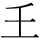
\includegraphics[width=3.8mm]{Chapter5/thengXkai.png}
 (09-17/09-01) provides evidence for the
change *k.l{\sil{ˤ}} \textgreater{} 見  \emph{k}- in type A syllables. Baxter \&
Sagart appear not to give examples of this sound change in type B
syllables.

\begin{description} \item
巠(
\includegraphics[width=3mm]{Chapter5/keng.png})  \emph{keng} \textless{} *k.l{\sil{ˤ}}- (09-01/0831a)
\item

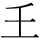
\includegraphics[width=3.8mm]{Chapter5/thengXkai.png}
(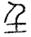
\includegraphics[width=4mm]{Chapter5/thengX.jpg})  
\emph{thengX} \textless{} *l̥- (09-17/0835a)
\item
梃  \emph{dengX} \textless{} *l{\sil{ˤ}}- (09-17/0835j)
\item
桯  \emph{yeng} \textless{} *l- (09-17/0835y)
\end{description}

§b. The series based on 丂 (13-03/13-43) provides evidence for the
change *k.r̥{\sil{ˤ}}- \textgreater{} 溪~ \emph{kh}- in type A syllables. Baxter
\& Sagart appear not to give examples of this sound change in type B
syllables.

\begin{description} \item
考  \emph{khawX} \textless{} *k.r̥{\sil{ˤ}}- (13-03d)
\item
老  \emph{lawX} \textless{} *r{\sil{ˤ}}- (13-43a)
\end{description}

§c. Baxter \& Sagart normally reconstruct a series that shows
 \emph{xiéshēng} contacts between velars and glottals as deriving from
inherited uvulars (cf. §). However, they also permit a pre-initial *k-
before {\sil{*ʔ-}} as an alternative explanation for such  \emph{xiéshēng}
series. They take the series based on 鬼(
\includegraphics[width=2mm]{Chapter5/kjwijX.png}) (28-01/28-09) as evidence
for the change {\sil{*k.ʔ-}} \textgreater{} 見  \emph{k}- (2014: 151).

\begin{description} \item
鬼(
\includegraphics[width=2mm]{Chapter5/kjwijX.png})  \emph{{\sil{kjwɨjX}}} \textless{} {\sil{*k.ʔ-}} (28-01/0569a)
 \item
畏(
\includegraphics[width=2.5mm]{Chapter5/'jwijH.png})  \emph{'{\sil{jwɨj}}H} \textless{} {\sil{*ʔ-}} (28-09/0573a)
\end{description}

Baxter \& Sagart make little effort to explain how they decide whether a
 \emph{xiéshēng} series should be analyzed as uvular initial versus
glottal initial with the occasional *k- prefix. It appears they prefer
not to have two  \emph{xiéshēng} series that write the same type of Old
Chinese syllable; by proposing {\sil{*k.ʔ-}} as the origin of 見  
\emph{k}- in the
reading of 鬼 \emph{{\sil{kjwɨjX}}} they are able to understand the series built
on 鬼 as encoding Old Chinese syllables of the shape *ʔuj as opposed to
the series built on 貴 as, which encodes Old Chinese syllables of the
shape *Quj \citep[151 n. 79 on p. 391]{Baxter2014OldChinese}. The inclusion
of readings with initial 曉 \emph{x}- and 以  \emph{y}- in the series
built on 貴 (31-02) essentially compels one to understand this series as
uvular initial in Baxter \& Sagart's system.\footnote{In violation of
  the \emph{xiéshēng} hypothesis, Baxter \& Sagart reconstruct many of
  the readings in the series built on 貴 (31-02) as having velar
  initials. e.g. 簣 \emph{khweajH} \textless{} *{\sil{kʰ}}{\sil{ˤ}}r- (31-02j), 聵
  \emph{ngweajH} \textless{} *[ŋ]{\sil{ˤ}}r- (31-02p). To my knowledge they
  have given no account of these reconstructions, but an obvious
  explanation to consider is that characters with velar readings are
  younger coinages, created after uvulars had already vanished.}

\begin{description} \item
靧  \emph{xwojH} \textless{} {\sil{*qʰ}}{\sil{ˤ}}- (31-02f)
\item
遺  \emph{ywij} \textless{} *{\sil{ɢ}}(r)- (31-02m)
\end{description}

§d. For *k- before resonants see §.

\paragraph{Tight pre-initials \textbf{*t-}}:
Tight pre-initial *t- explains the appearance of Middle Chinese
pronunciations with dental (\emph{shétóu} 舌頭  \emph{T}-),\footnote{Although
  Baxter \& Sagart include *t.q{\sil{ˤ}}- \textgreater{} 端  \emph{t}- in the
  table that summarizes the correspondences involving *t- (2014: 157), I
  am unable to locate an explicit discussion of this change in their
  volume.} palatal (\emph{zhāngzǔ} 章組  \emph{Tsy}-), or retroflex
initials (\emph{shéshǎng}舌上 \emph{Tr}-) in series that do not
predominantly contain readings with these initials 
\citep[157-159]{Baxter2014OldChinese}.

§a. The series based on 九(
\includegraphics[width=3mm]{Chapter5/kjuwX.png}) (04-12/13-23) provides evidence for the
change *t.kr- \textgreater{} 知 \emph{tr}-.

\begin{description} \item
肘(
\includegraphics[width=2mm]{Chapter5/trjuwX.png})  \emph{trjuwX} \textless{} *t.kr- (13-23a)
\item
九(
\includegraphics[width=3mm]{Chapter5/kjuwX.png})  \emph{kjuwX} \textless{} *k- (04-12a)
\end{description}

§b. The series based on 出 (31-16) provides evidence for the change
*t-{\sil{kʰ}}- \textgreater{} 昌 \emph{tsyh}- in type B syllables.

\begin{description} \item
出  \emph{tsyhwit} \textless{} *t.{\sil{kʰ}}- (31-16a)
\item
掘  \emph{gjut} \textless{} *g- (31-16s)
\end{description}

§c. The series based on 巠 (09-01) provides evidence for the change
*t.{\sil{kʰ}}r- \textgreater{} 徹 \emph{trh}- in type B syllables.

\begin{description} 
\item
徑  \emph{kengH} \textless{} *{\sil{kˤ}}- (09-01f)
\item

\includegraphics[width=3.4mm]{Chapter5/khengH.png}
 \emph{khengH} \textless{} *{\sil{kʰ}}{\sil{ˤ}}- (09-01j)
\item
陘  \emph{heng} \textless{} *g{\sil{ˤ}}- (09-01l)
\item
牼  \emph{kheang} \textless{} *{\sil{kʰ}}{\sil{ˤ}}r- (09-01q)
\item
䞓  \emph{trhjeng} \textless{} *t.{\sil{kʰ}}r- (09-01x)
\end{description}

§d. For *t- before resonants see §.

\paragraph{Tight stop pre-initials before
resonants}: Before resonants divergent dialect treatment of *p-, *t-,
and *k- on the way to Middle Chinese often leads to alternate readings
of the same character (Baxter \& Sagart 2014: 162).

\begin{description} \item
稟 (38-19a)  \emph{pimX} \textless{} *pr- \textless{} *p.r-, versus
 \emph{limX} \textless{} *p.r-
\item
慹 (37-08h)  \emph{tsyip} \textless{} *t- \textless{} *t.n-, versus
 \emph{nep} \textless{} *n{\sil{ˤ}}- \textless{} *t.n{\sil{ˤ}}-
\item
袂 (20-03d) \emph{kwe}t \textless{} *{\sil{kʷˤ}}- \textless{} *k.m{\sil{ˤ}}-, versus
 \emph{mjiejH} \textless{} *m- \textless{} *k.m-
\end{description}

\paragraph{Tight nasal pre-initials *m- and
*N-:} On the basis of  \emph{xiéshēng} evidence the tight
pre-initials *m- and *N- before obstruents are not easily distinguished
from each other nor are they distinguishable from simplex voiced
consonants. Nonetheless, *m-/*N- can be isolated on the basis of
 \emph{xiéshēng} evidence before the uvulars {\sil{*qʰ}}- and *{\sil{ɢ}}- (§a) and before
*r- (§b). In addition, *m- is identifiable on the basis of
 \emph{xiéshēng} evidence before (non-labial) nasals (§c).

§a. The pre-initials *m- and *N- before some uvulars are together
distinguishable from the voiced uvular *{\sil{ɢ}}- on the basis of
 \emph{xiéshēng} evidence. For example, the series built on 牙( )
(01-34/01-45) exhibits connections typical of a uvular series (見
 \emph{k}-, 影  \emph{'}-, 以 \emph{y}-), but it also contains readings
that begin with 疑  \emph{ng}-. One would like to find a way to credit
this 疑  \emph{ng}- also to an erstwhile uvular. Baxter \& Sagart's
explanation is a prefix *m- or *N- before a voiced uvular *{\sil{ɢ}} or the
voiceless aspirated uvular {\sil{*qʰ}}-, with the merger *m-{\sil{qʰ}}-, *m-ɢ-, *N-{\sil{qʰ}}-,
*N-ɢ- \textgreater{} 疑 \emph{ng}- (2014: 128-131). There is no way to
decide on the basis of  \emph{xiéshēng} evidence alone which of the four
uvular sources of 疑 \emph{ng}- is the correct re­con­struc­tion for a
given word.

\begin{description} \item
牙(
\includegraphics[width=2mm]{Chapter5/ngae.png} ) \emph{ngae} \textless{} *m.{\sil{qʰ}}r-, *m.ɢr-, *N.{\sil{qʰ}}r-, or *N.ɢr-
(01-34a)\footnote{\citet[131]{Baxter2014OldChinese} reconstruct this word
  with initial *m.{\sil{ɢˤ}}r-. It appears phonologically odd that *m.{\sil{qʰ}}-,
  *m.ɢ-, *N.{\sil{qʰ}}-, *N.{\sil{ɢ-}} develop to 疑  \emph{ng}-, but that *m.q- and
  *N.q- merge with *{\sil{ɢ}}-.}

\item
鴉  \emph{'ae} \textless{} q{\sil{ˤ}}r- (01-34h)

\item
舉(
\includegraphics[width=2.5mm]{Chapter5/kjoX.png}) \emph{kjoX} (01-45a)
\item
與(
\includegraphics[width=2.5mm]{Chapter5/yoX.png}) \emph{yoX} \textless{} *{\sil{ɢˤ}}(r)- (01-45b)\footnote{Baxter \& Sagart
  (2014: 125) in fact reconstruct this word with initial *m-q(r)-
  relying on Mĭn evidence (cf. §a).}
\end{description}

§b. \citet[122, 133-134]{Baxter2014OldChinese}
%Baxter \& Sagart (2014: 122, 133-134) 
reconstruct *N.r- and *m.r-,
both merging with *l- (\textgreater{} 以  \emph{y}-), in order to account
for contacts between 以  \emph{y}- and 來  \emph{l}-. For example, the
character 斿 (13-33a) has the two readings  \emph{yuw} (\textless{} *l-
\textless{} *N.r- or *m.r-) and \emph{ljuw} (\textless{} *r-).\footnote{Baxter
  \& Sagart (2014: 134) postulate that Middle Chinese shows a mixture of
  two dialect developments. In one dialect *m.r- develops similarly to
  *l- (cf. 蠅  \emph{ying} \textless{} *m.r- {[}06-24a] and 黽
   \emph{meangX} \textless{} *m{\sil{ˤ}}r- {[}06-24d]). In the other dialect
  *m.r- merges with *m- (cf. 命  \emph{mjaengH} \textless{} *m.r-
  {[}09-32a] and 令  \emph{ljeng} \textless{} *r- {[}09-19a]). As
  reconstructing 命  \emph{mjaengH} with *mr- rather than *m.r- seems
  explanation enough, I am unable to follow their reasoning for the need
  to distinguish two dialect developments. One may further wonder what
  exact phonetic difference they suppose the notation *mr- versus *m.r-
  to reflect. }

§c. One context in which *m- makes its presence observable in
 \emph{xiéshēng} relationships is before the (non-labial) nasals *ŋ- and
*n-. Baxter \& Sagart reconstruct the Old Chinese clusters *m.ŋ- and
*m.n- (\textgreater{} 明 \emph{m}-) (2014: 132-133); these clusters
provide an ex­pla­na­tion for the occasional intrusion of 明
 \emph{m}-\emph{ }initial word into a series that predominantly has
initial 疑~ \emph{ng}- or 泥~ \emph{n}-. The series built on 兒 (07-11)
exhibits 明~ \emph{m}- in a 疑~ \emph{ng}- series.

\begin{description} \item
兒 \emph{nye} \textless{} *ŋ- (07-11a)
\item
倪 \emph{ngej} \textless{} *ŋ{\sil{ˤ}}- (07-11f)
\item
麑 \emph{mej} \textless{} *m.ŋ{\sil{ˤ}}- (07-11o)
\end{description}

The series built on 爾 (07-20) exhibits 明~ \emph{m}- in an 泥~ \emph{n}-
series.

\begin{description} \item
爾 \emph{nyeX} \textless{} *n- (07-20a)
\item
嬭 \emph{nejX} \textless{} *n{\sil{ˤ}}- (07-20d)
\item
彌 \emph{mjieX} \textless{} *m.n- (07-20m)
\end{description}

\paragraph{Tight pre-initials before uvulars
as a source of Middle Chinese velars :} 
\label{par:t-p-initials-before-ufvulars-as-a-source-of-MC-velars}
As discussed above, Baxter \&
Sagart reconstruct series that mix glottals and velars as uvulars (§),
but the discussion so far has not treated the velar stops appearing in
such series. Baxter \& Sagart propose that tightly attached stop
pre-initials are the origin of velar initial readings appearing in
uvular series (\citet[28, 45, 168-170]{Baxter2014OldChinese})\footnote{Sagart
  \& Baxter (2009: 231) proposed that `loose' pre-initials conditioned
  the shift from uvulars to Middle Chinese velars, but because some of
  the relevant words do not have `softened' initials in proto-Mǐn they
  have revised their proposal to instead suggest `tight' pre-initials
  before uvulars are the source of the relevant cases of velars (Baxter
  \& Sagart 2014: 385 note 24). For tight pre-initial *N- and *s- before
  uvulars see respectively §a and §e-g.}

§a. The series built on 公 (12-13) provides evidence of *C.q{\sil{ˤ}}- and the
change *C.q{\sil{ˤ}}- \textgreater{} 見~ \emph{k}- in type A syllables.

\begin{description} \item
公(
\includegraphics[width=3mm]{Chapter5/kuwng.png}) \emph{kuwng} \textless{} *C.q{\sil{ˤ}}- (12-13/1173a)
\item
瓮 `\emph{uwngH} \textless{} {\sil{*qˤ}}- (12-13g)
\item
容(
\includegraphics[width=4mm]{Chapter5/yowng.png}) \emph{yowng} \textless{} *{\sil{ɢ}}r- (12-11a)
\end{description}

§b. The series built on 京 (03-10) provides evidence of *C.qr- and the
change *C.qr- \textgreater{} 見~ \emph{k}- in type B syllables.

\begin{description} \item
景 \emph{kjaengX} \textless{} *C.qr- (03-10/0755d)
\item
影 \emph{'jaengX} \textless{} *qr- (03-21/0756a)
\end{description}

§c. The series built on 衍 (24-29) provides evidence of *C.{\sil{qʰ}}r- and the
change of *C.{\sil{qʰ}}r- \textgreater{} 溪~ \emph{kh}- in type B syllables.

\begin{description} \item
衍  \emph{yenH} \textless{} *N-q(r)- (24-29/24-29a)\footnote{Baxter \&
  Sagart reconstruct *N-q(r)- rather than *{\sil{ɢ}}- on the presumption that 愆
  *C.{\sil{qʰ}}ra[n] \textgreater{}  \emph{khjen} `exceed, err' and 衍
  *N-q(r)anʔ \textgreater{}  \emph{yenX} `overflow' derive from the same
  root (2014: 169).}

\item
愆 \emph{khjen} \textless{} *C.{\sil{qʰ}}r- (24-29/24-29b)
\end{description}

§d. The series built on 气 (30-01) provides evidence of *C.{\sil{qʰ}}- and the
change *C.{\sil{qʰ}}- \textgreater{} 溪~ \emph{kh}- in type B syllables.

\begin{description} \item
乞 \emph{{\sil{khjɨ}}t} \textless{} *C.{\sil{qʰ}}- (30-01/0517f)
\item
氣 \emph{{\sil{xjɨj}}H} \textless{} {\sil{*qʰ}} (30-01/0517c)
\end{description}

§e. The series built on 吅 provides evidence of *C.{\sil{qʷʰ}}- and the change
*C.{\sil{qʷʰ}}- \textgreater{} 溪~ \emph{kh}- 
\citep[170]{Baxter2014OldChinese}.

\begin{description} \item
吅 \emph{xjwon} \textless{} {\sil{*qʷʰ}}- (25-02/0158-)
\item
勸 \emph{khjwonH} \textless{} *C.{\sil{qʷʰ}}- (25-02/0158s)
\end{description}

§f. A sequence of *m- or *N- and a uvular give rise to initial
疑~ \emph{ng}- (cf. §a).

\subsection{Reconstructing tight pre-initials on the basis of
morphological
speculation}

\paragraph{} 
\label{par:recon-t-p-initials-on-morphological-speculation}
Baxter \& Sagart reconstruct seven morphological affixes: the
prefixes *s-, *N-, *m-, *t-, and *k-, an infix *-r-, and a suffix *-s
(2014: 53-59, cf. §§-). They distinguish between a verb valence
increasing *s- prefix and a circumstantial noun *s- prefix (2014: 56).
Their prefix *N- decreases verb valence (2014: 54, cf. §§-).\footnote{Both
  Ancient Egyptian and the Semitic languages also evince an *s- valence
  increasing and *N- valence decreasing prefix (Moscati 1964: 125-127).
  This is a remarkable morphological coincidence between Old Chinese, as
  Baxter \& Sagart reconstruct it, and Afro-Asiatic. } They distinguish
five different *m- prefixes (2014: 54-56, cf. § and §). The presumed *t-
prefix they do not use to explain relationships between words, but
simply note its occurrence in some words (2014: 56-57); they never
reconstruct the pre-initial *t- on the basis of morphological
speculation.\footnote{The pair 臭  \emph{tsyhuwH} \textless{} *t-{\sil{qʰ}}u(ʔ)-s
  (13-12a) `foul smell ` and 朽  \emph{xjuwX} \textless{} {\sil{*qʰ}}(r)uʔ
  (13-03m) `rot, decay' is perhaps the one case in which they presume a
  pre-initial *t- on the basis of etymological speculation (Baxter \&
  Sagart 2014: 57). However, they do not discuss the pair explicitly, so
  one cannot be sure on what grounds they reconstruct initial 昌
   \emph{tsyh}- as *t-{\sil{qʰ}} in the first word. For example, one might regard
  the series built on 臭 (13-12) as uvular because of the velar
  fricative initial of 嗅 \emph{xjuwH} (13-12c), cf. §§-. } The presumed
prefix *k- nominalizes verbs (2014: 57, cf. §). The infix *-r- and final
*-s are reconstructed using the conventional sources for Old Chinese
historical phonology; Baxter \& Sagart assign them with a morphological
meaning, but, unlike for the prefixes, do not employ morphological
argumentation to posit their existence.

\paragraph{The tight pre-initial
*s-:} All researchers appears to concur that *s- had a
causative function in Old Chinese (cf. Handel 2012). The credit for this
proposal, as well as a proposed link between *s- in Chinese and the
Tibetan causative prefix \emph{s}-, typically goes to Conrady (1896).
However, Conrady did not propose Chinese *s- in the circumstances in
which Karlgren, Li, Baxter, and Sagart do, but rather in those places
where Baxter \& Sagart would reconstruction voiceless nasals (see
Conrady 1896: 156).

Baxter \& Sagart propose two different morphological functions for an
*s- prefix, a valency increasing verb prefix and a prefix that ``derives
circumstantial nouns (place, time, instrument)'' (2014: 56). Outside of
the initial presentation of the two prefixes, in their discussion of
words presumed to have an etymological relationship Baxter \& Sagart
generally fail to make explicit which of the two *s- prefixes they
believe is at play. They employ etymological arguments in favor of *s-
prefix origins of Middle Chinese 心~ \emph{s}- (cf. §), 生~ \emph{sr}-
(cf. §), 邪~ \emph{z}- (cf. §), 精~ \emph{ts}-, 莊~ \emph{tsr}- (cf. §),
清~ \emph{tsh}- (cf. §), and 初~ \emph{tsrh}- (cf. §).

§a. They provide the following four pairs of words to exemplify the
valency increasing prefix.

\begin{description} \item
烝 \emph{tsying} \textless{} *təŋ (06-10h) `rise (of steam)'; 升
 \emph{sying} \textless{} *s-təŋ (06-16a) `lift up, to save, to present
to'
\item
諤 \emph{ngak} \textless{} *ŋ{\sil{ˤ}}ak (02-14k) `speak frankly'; 愬 \emph{suH}
\textless{} *s-ŋ{\sil{ˤ}}ak-s (02-34b) `complain, accuse'
\item
當 \emph{tang} \textless{} *t{\sil{ˤ}}aŋ (03-32q) `match (v.); have the value
of, rank with'; 商 \emph{syang} \textless{} *s-taŋ (03-40a) `estimate'
\item
視 \emph{dzyijX} \textless{} *gijʔ (26-07h) `look, see'; 示 \emph{zyijH}
\textless{} *s-gijʔ-s (26-07a) `show (v.)'
\end{description}

§b. They provide the following three pairs of words to exemplify the
circumstantial noun prefix.\footnote{Baxter \& Sagart also give an
  example of the circumstantial noun prefix, in which the prefix is
  loose, viz. 以  \emph{yiX} \textless{} *ləʔ `take, use', 鈶 \emph{ziX}
  \textless{} *sə.ləʔ `handle of plow or sickle ` (i.e. `instrument of
  holding') (2014: 56).}

\begin{description} \item
屰 \emph{ngjaek} \textless{} *ŋrak (02-14a) `go against, reverse'; 朔
 \emph{sraewk} \textless{} *s-ŋrak (02-34a) `first day of month' (when
the moon changes from waning to waxing) (cf. p. n. )
\item
通 \emph{thuwng} \textless{} *l̥{\sil{ˤ}}oŋ (12-10r) `penetrate'; 窗
 \emph{tsrhaewng} \textless{} *s-l̥{\sil{ˤ}}roŋ (12-19-) `window' (i.e. `where
light penetrates')
\item
亡 \emph{mjang} \textless{} *maŋ (03-65a) `flee; disappear; die'; 喪
 \emph{sang} \textless{} *s-m{\sil{ˤ}}aŋ (03-54a) `mourning, burial' (i.e.
'circumstances associated with death')
\end{description}

The second and third example of the circumstantial noun prefix are not
flawless. The derivation of 窗  \emph{tsrhaewng} \textless{} *s-l̥{\sil{ˤ}}roŋ
`window' from 通  \emph{thuwng} \textless{} *l̥{\sil{ˤ}}oŋ `penetrate' involves an
-r- infix in addition to the *s- prefix and the derivation from of 喪
 \emph{sang} \textless{} *s-m{\sil{ˤ}}aŋ `mourning, burial' from 亡~ \emph{mjang}
\textless{} *maŋ `flee; disappear; die' includes an unexplained change
from a type B syllable to a type A syllable.

\paragraph{Tight pre-initial *s- as an origin
of Middle Chinese 心~} \emph{\textbf{s}}\textbf{-}\textbf{:} On
the basis of etymological argumentation Baxter \& Sagart reconstruct
both *s.ts- (cf. §a) and *s.ts{\sil{ʰ}}{\sil{ˤ}}- (§b) as origins for 心~ \emph{s}-.

§a. Baxter \& Sagart offer two pair of etymologically related words in
support of a change *s.ts- \textgreater{} 心~ \emph{s}- 
\citeyearpar[136]{Baxter2014OldChinese}.

\begin{description} \item
節 \emph{tset} \textless{} *ts{\sil{ˤ}}ik (29-30e) `joint of bamboo'; 膝
 \emph{sit} \textless{} *s.tsik (29-32c) `knee'
 \item
㕚 , 爪  \emph{tsraewX} \textless{} *[ts]{\sil{ˤ}}ruʔ (13-60a, 13-59a)
`claw'; 搔  \emph{saw} \textless{} *s-{[}ts]{\sil{ˤ}}u (13-60f) `scratch (v.)'
\end{description}

These proposals are not without difficulties. The derivation of `knee'
from `joint of bamboo' is neither an instance of the valence increasing
prefix nor of the circumstantial noun prefix. Sagart \& Baxter instead
suggest that perhaps ``we have a Chinese instance of the
T{[}ibeto-]B{[}urman] *s- animal (and body-part?) prefix from TB
*sya -- `flesh''' (2012: 45), which Benedict (1972: 106) has proposed. I
concur with Chang that Benedict's animal prefix is ``a dubious
proposition'' (1973: 336).\footnote{The fact that `joint of bamboo' is
  type A whereas `knee' is type B further complicates the relationship
  between the two words. There are other examples of alternations
  between type A and type B words (Baxter \& Sagart 1997: 61-62), with
  the pair 內 \emph{nop} \textless{} *n{\sil{ˤ}}{[}u]p `bring or send in'
  (37-16e) and 入 \emph{nyip} \textless{} *n{[}u]p `enter' (37-16a) as
  a well known case. No explanation has been put forward for the origin
  or derivational meaning of such patterns.} The proposal to derive
'scratch' from `claw' with a denominative *s- is less problematic, but
the absence of medial -r- in the verb `scratch' is an obstacle to this
proposal.

§b. Baxter \& Sagart offer one pair of etymologically related words in
support of a change *s.ts{\sil{ʰ}}{\sil{ˤ}}- \textgreater{} 心~ \emph{s}- 
\citeyearpar[139]{Baxter2014OldChinese}.

\begin{description} \item
清 \emph{tshjeng} \textless{} *ts{\sil{ʰ}}eŋ `clear (adj.)'; 星  \emph{seng}
\textless{} *s-ts{\sil{ʰ}}{\sil{ˤ}}eŋ `star' (i.e. that which is bright)
\end{description}

They acknowledge the difficulty that `clear' is type B whereas `star' is
type A. This proposed pair of cognates would not be compelling except
that words for `star' in the Mǐn dialects support initial *tsh- (cf.
Amoy /ts{\sil{ʰ}}ĩ 1/, §).

\paragraph{Tight pre-initial *s- as an origin of Middle Chinese
生 \emph{sr-}:} On the basis of the following pair of
words, Baxter \& Sagart reconstruct *s-{\sil{qʰ}}r- as one source of Middle
Chinese 生  \emph{sr}- 
\citeyearpar[129]{Baxter2014OldChinese}.

\begin{description}
\item
許 \emph{xjoX} \textless{} {\sil{*qʰ}}(r)aʔ (01-30i) `place (n.)'; 所
 \emph{srjoX} \textless{} *s-{\sil{qʰ}}raʔ (01-63a) `place (n.); that which'
\end{description}

Without further discussion this derivation is unconvincing. Note however
that the line 伐木許許 "chop trees `hack-hack'" of Ode 165.2 is quoted
in the entry for the character 所 in the 說文解字  \emph{Shuōwén Jiězì}
as 伐木所所; thus, the pronunciations of 許 (01-30i) and 所 (01-63a)
must have had very similar pronunciations, or at least both reflected
pronunciations that were suitable as onomatopoeia for the sound of
chopping wood.\footnote{I thank Adam Smith for drawing my attention to
  this use of 許 (01-30i) and 所 (01-63a) (\emph{per litteras} 25 May
  2017).}

\paragraph{Tight pre-initial *s- as an origin
of Middle Chinese 邪 \emph{\textbf{z}}\textbf{-:}} 
\label{par:tight-pre-initial-s-for-MC-z-2}
\citet[141-142]{Baxter2014OldChinese}
propose that pre-initial *s- before voiced obstruents in
type B syllables is one source of Middle Chinese 邪 \emph{z}-. They
propose *s.ɢ- \textgreater{} 邪  \emph{z}- on the basis of
 \emph{xiéshēng} evidence (cf. §a). They also propose *s.d-
\textgreater{} 邪  \emph{z}- on the basis of proto-Mǐn and loanwords into
non-Sinitic languages (cf. §). For the parallel, but yet more
complicated *s-m-t- \textgreater{} 邪  \emph{z}- they return to
etymological argumentation.

\begin{description} \item
著 \emph{trjak} \textless{} *trak (01-38n') `place (v.)'; 席  \emph{zjek}
\textless{} *s-m-tAk (02-29a) `mat' (i.e. `place for putting things')
\end{description}

Baxter \& Sagart do not however account for the morphological function
of the *m- prefix in `mat' nor the -r- infix in `place (v.)'.

\paragraph{Tight pre-initial *s- as an origin of Middle Chinese
\textbf{船}  \emph{\textbf{zy}}-: }In favor of the change *s.g-
\textgreater{} \textbf{船}  \emph{zy}- 
\citet[56]{Baxter2014OldChinese} point the the following verb pair.

\begin{description} \item
視 \emph{dzyijX} \textless{} *gijʔ (26-07h) `look, see'; 示  \emph{zyijH}
\textless{} *s-gijʔ-s (26-07a) `show (v.)'\footnote{Handel (2012: 76)
  points out that this pair is the only example of a causative *s-
  prefix before non-resonant velar initials in Baxter \& Sagart's
  system.}
\end{description}

\paragraph{Tight pre-initial *s- as an origin
of Middle Chinese \textbf{精~} \emph{ts}- and
莊~ \emph{tsr}-:}
Baxter \& Sagart (2014:
136) propose a change *s.t{\sil{ˤ}}- \textgreater{} 精~ \emph{ts}- on the basis
of presumed etymological relationships between words with Middle Chinese
initial 端 \emph{t}- and those with initial 精~ \emph{ts}-.

\begin{description} \item
登 \emph{tong} \textless{} *t{\sil{ˤ}}əŋ (06-09e) `ascend'; 增 \emph{tsong}
\textless{} *ts{\sil{ˤ}}əŋ \textless{} *s-t{\sil{ˤ}}əŋ (06-19c) `increase (v.)'
\end{description}

Baxter \& Sagart (2014: 136) similarly propose a change *s-t{\sil{ˤ}}r-
\textgreater{} 莊~ \emph{tsr}- on the basis of presumed etymological
relationships between words with Middle Chinese initial 知  \emph{tr}-
and those with initial 莊~ \emph{tsr}-.

\begin{description} \item
謫 \emph{treak} \textless{} *t{\sil{ˤ}}rek (07-12r) `blame (v.)';\footnote{Baxter
  \& Sagart in fact reconstruct 謫 \emph{treak} \textless{} *C.t{\sil{ˤ}}rek
  (07-12r) `blame (v.)', positing the *C. pre-initial on the basis of
  Vietnamese  \emph{dức} {[}zɯk D1] `reprove' (2014: 136). } 責
 \emph{tsreak} \textless{} *ts{\sil{ˤ}}rek \textless{} *s-t{\sil{ˤ}}rek (08-14m) `demand
payment'
\end{description}

The derivation from `blame' to `demand payment' is not obviously a case
of valence increase.

\paragraph{Tight pre-initial *s- as an origin
of Middle Chinese 清\textbf{~} \emph{\textbf{tsh}}\textbf{-:
}}Baxter \& Sagart propose the change *s.r̥{\sil{ˤ}}- \textgreater{}
清~ \emph{tsh}- to account for Middle Chinese doublets in which one word
begins with 清~ \emph{tsh}- and the other with 生~ \emph{sr}-; they credit
these doublets to divergent dialect developments (2014: 150).

\begin{description} \item
採 \emph{tshojX} \textless{} *s.r̥{\sil{ˤ}}əʔ (04-44d) `pluck, reap'; 嗇
 \emph{srik} \textless{} *s.rək (04-44d) `reap'
 \item
彩 \emph{tshojX} \textless{} *s.r̥{\sil{ˤ}}əʔ (04-44a) `colorful'; 色  \emph{srik}
\textless{} *s.rək (05-31a) `color; countenance'
\end{description}

\paragraph{Tight pre-initial *s- as
an origin of Middle Chinese
初~ \emph{tsrh}-:} Baxter \& Sagart
propose a change *s-t{\sil{ʰ}}{\sil{ˤ}}- \textgreater{} 初~ \emph{tsrh}- on the basis of
the following verb pair, in which they see the valence increasing *s-
prefix at play.

\begin{description} \item
推 \emph{thwoj} \textless{} *t{\sil{ʰ}}{\sil{ˤ}}uj (28-11a') `push away'; 催
 \emph{tshwoj} \textless{} *s-t{\sil{ʰ}}{\sil{ˤ}}uj (28-11j') `urge, repress'
\end{description}

\paragraph{The tight nasal p}re-initial *m-
and\textbf{*N-:} The nasal prefixes *m- and *N- of Baxter \& Sagart's
system are almost always impossible to distinguish using  \emph{xiéshēng}
evidence; in addition, before stops using  \emph{xiéshēng} evidence they
are indistinguishable from plain voiced onsets. Nonetheless, presumed
morphology, as well as proto-Mǐn (cf. §) and loanwords into Vietnamese
(cf. §), allow these two pre-initials to be differentiated from each
other and from voiced stops in many circumstances.

\paragraph{Pre-initial *N-}: To explains
morphological alternations between transitive and intransitive verbs
Pulleyblank (1973: 114) proposed a prefix (that he reconstructed *ɦ)
which voices a voiceless initial while making a verb intransitive. Often
both the transitive and the intransitive verb are written with the same
character.

\begin{description} \item
見 (23-02a) \emph{kenH} `see',  \emph{henH} `appear'
 \item
敗 (21-35f) \emph{paejH} `defeat',  \emph{baejH} `suffer defeat'
\item
壞 (28-06d) \emph{kweajH} `destroy, ruin',  \emph{hweajH} `be destroyed'
\item
斷 (25-22a) \emph{twanX} `cut in two',  \emph{dwanX} `be cut in two'
\item
折 (21-19a) \emph{tsyet} `break, bend' (v.t.),  \emph{dzyet} `bend'
(v.i.)
\end{description}

Sagart (1993: 244) proposed that the Chinese intransitive voicing prefix
must be some kind of nasal on the basis of the Mien high tone voiced
initial in the Chinese loanword 折 dzɛ́ʔ `be cracked', which suggests a
proto-Yao pre-nasalized voiceless initial. Baxter \& Sagart have changed
little in their evidence for and explanation of *N- since 1997 (cf.
Baxter \& Sagart 1997: 45-47). In their recent book they present the
following verb pairs as evidence of *N- (2014: 116-123).

\begin{description} \item
見  \emph{kenH }\textless{} *[k]{\sil{ˤ}}en-s (23-02a) `see'; 見 \emph{henH}
\textless{} *N-{[}k]{\sil{ˤ}}en-s (23-02a) `appear'
\item
敗  \emph{paejH} \textless{} *p{\sil{ˤ}}ra{[}t]-s (21-35f) `defeat'; 敗
 \emph{baejH} \textless{} *N-p{\sil{ˤ}}ra{[}t]-s (21-35f) `suffer defeat'
\item
壞  \emph{kweajH} \textless{} *[k]{\sil{ˤ}}ruj-s (28-06d) `destroy, ruin'; 壞
 \emph{hweajH} \textless{} *N-{[}k]{\sil{ˤ}}ruj-s (28-06d) `be destroyed'
\item
斷  \emph{twanX} \textless{} *t{\sil{ˤ}}o[n]ʔ (25-22a) `cut in two'; 斷
 \emph{dwanX} \textless{} *N-t{\sil{ˤ}}o[n]ʔ (25-22a) `be cut in two'
\item
折  \emph{tsyet} \textless{} *tet (21-19a) `break, bend' (v.t.); 折
 \emph{dzyet} \textless{} *N-tet (21-19a) `bend' (v.i.)
\item
夾  \emph{keap} \textless{} *C.{\sil{kˤ}}rep (35-03a) `press between'; 狹
 \emph{heap} \textless{} *N-{\sil{kˤ}}rep (35-03e) `narrow'
\item
置  \emph{triH} \textless{} *trək-s (05-12g) `put, place; set upright';
直 \emph{drik} \textless{} *N-trək (05-12a) `straight'
\item
清  \emph{tshjeng} \textless{} *ts{\sil{ʰ}}eŋ (09-25i') `clear (adj.)'; 晴
 \emph{dzjeng} \textless{} *N-ts{\sil{ʰ}}eŋ (09-25-) `clear (of weather)'
\end{description}

§a. To explain apparent etymological connections between words with
Middle Chinese initial 以  \emph{y}- or  \emph{d}- (normally from OChi.
*l-) and Middle Chinese initial \emph{l}- (from OChi. *r-), Baxter \&
Sagart (2014: 122) posit an original *N-r- that merges with *l- (i.e.
OChi. *N-r- \textgreater{} *l- \textgreater{} MChi. 以  \emph{y}- and
OChi. *N-r{\sil{ˤ}}- \textgreater{} *l{\sil{ˤ}}- \textgreater{} MChi.  \emph{d}-).

\begin{description} \item
流  \emph{ljuw} \textless{} *ru (13-46a) `flow (v.)'; 游 \emph{yuw}
\textless{} *lu \textless{} *[N-]ru (13-33f) `float, swim'
\item
旒  \emph{ljuw} \textless{} *[r]u (13-46c) `pendants of a banner or
cap'; 斿 \emph{yuw} \textless{} *lu \textless{} *[N.]ru (13-33a)
`pendants of a banner'
\item
儽  \emph{lwojH} \textless{} *[r]{\sil{ˤ}}uj-s (28-15p) `exhausted'; 隤
 \emph{dwoj }\textless{} *l{\sil{ˤ}}wəj \textless{} *N-r{\sil{ˤ}}uj (28-13a) `exhausted'
\item
婪  \emph{lom} \textless{} *[r]{\sil{ˤ}}{[}ə]m (38-18i) `covet'; 淫
 \emph{yim} \textless{} *ləm \textless{} *N.r{[}ə]m (38-15b) `excess;
licentious'
\end{description}

Baxter \& Sagart find no reason to reconstruct *N- before voiceless
resonants (2014: 122).

§b. Before uvulars the prefix *N- induces a velar nasal initial (Baxter
\& Sagart 2014: 121).

\begin{description} \item
嚇  \emph{xaek} \textless{} {\sil{*qʰ}}{\sil{ˤ}}rak (02-10b) `to frighten'; 愕
\emph{ngak} \textless{} *N-{\sil{qʰ}}{\sil{ˤ}}ak (02-14h) `scared'
\item
夏  \emph{haeX} \textless{} *{\sil{[ɢ]ˤ}}raʔ (01-15a) `great'; 雅
 \emph{ngaeX} \textless{} *N-{\sil{ɢˤ}}raʔ (01-34g) `proper, refined'
\end{description}

The hypotheses *N-{\sil{qʰ}} \textgreater{} \emph{ng-} and *N-ɢ \textgreater{}
 \emph{ng}- also receive support from  \emph{xiéshēng} evidence (§a).

\paragraph{Pre-initial *m-:} Baxter \& Sagart
propose a number of morphological *m- prefixes in Old Chinese, including
a volitional verb prefix, a `human body part prefix', and an `animal
prefix' (2014: 54-56). The verbal prefix *m-, was the first *m- prefix
to emerge in their work, and it emerged as distinct from *N- only slowly
in their system. Some of Baxter's 1992 examples of *N- pair a noun with
a voluntary verb, rather than a transitive with an intransitive verb
(Baxter 1992: 218-219). Such cases instil the suspicion that there is a
morpheme other than the detransitivizing *N- at play.

\begin{description} \item
朝 (16-17a) \emph{trjew} `morning',  \emph{drjew} `(morning ceremony:)
audience, court, go to the court of'

\item
背 (05-32e) \emph{pwojH} `the back',  \emph{bwojH} `turn the back'
\end{description}

Sagart (1999a: 79-86) proposes a prefix *m- with volitional meaning. He
presents three examples with lateral initial verbs.

\begin{description} \item
順  \emph{zywinH} \textless{} *m-lun-s in 1999, now *Cә.lu[n]-s
(34-20c) `follow; obey' (cf. 循  \emph{zwin} \textless{} *sə.lu[n]
{[}34-21f] `follow')

\item
贖  \emph{zyowk} \textless{} *m-l{[}u]k in 1999, now *Cə.lok (14-14t)
'redeem' (cf. 賣 \emph{yuwk} \textless{} *luk {[}14-14a] `sell')

\item
射  \emph{zyek} \textless{} *m-lak in 1999, now *Cә.lAk (02-26a) `hit
with bow and arrow' (cf. 釋  \emph{syek} \textless{} *l̥Ak {[}02-25l]
'release; dissolve')
\end{description}

Baxter \& Sagart no longer reconstruct these three words with a *m-
pre-initial; whether or not they would still regard the comparisons made
(e.g. of 順 \emph{zywinH} `follow; obey' to 循  \emph{zwin} `follow') as
reflecting genuine etymological relationships is unclear.\footnote{It is
  worrying that the semantic affect of *m- has remained stable since
  1999 although the words that originally motivated these semantics are
  no longer taken as examples of this prefix. This paradox suggests that
  `volition' may be too broad a meaning, and allow for any number of
  potentially invalid etymological proposals.}

Nonetheless, Baxter \& Sagart have subsequently found quite a few of
potential examples of this *m- voluntary prefix. Although in Middle
Chinese (and Sinitic loans in Hmong-Mien) *N- and *m- are
indistinguishable, in proto-Mĭn and Sinitic loans into Vietic the two
prefixes can be distinguished (§ and §).\footnote{With regard to Chinese
  external evidence Sagart \& Baxter (2010) point to an \emph{m}- prefix
  in Daai Chin, as described by Hartmann 2001. Although `volition' does
  appear to cover well the examples that Hartmann presents, this is not
  her analysis of the prefix's function. Also compare So-Hartmann (2009:
  55-56).}

§a. Baxter \& Sagart propose an *m- prefix before voiceless stops on the
basis of apparent etymological relationships between Middle Chinese
words with voiced initials and those with voiceless initials (2014:
123).

\begin{description} \item
包 \emph{paew} \textless{} *p{\sil{ˤ}}ru (13-72a) `wrap, bundle'; 抱  \emph{bawX}
\textless{} *[m-p]{\sil{ˤ}}uʔ (13-72j) `carry in the arms' (volitional)

\item
拄 \emph{trjuX} \textless{} *troʔ (10-19e) `prop up, support (v.)'; 樹
 \emph{dzyuX} \textless{} *m-toʔ (10-22j) `plant (v.); place upright'
(volitional)

\item
合 \emph{kop} \textless{} *{\sil{kˤ}}op (37-01a) `together; put together;
combined'; 合 \emph{hop} \textless{} *m-{\sil{kˤ}}op (37-01a) `come together;
bring together' (volitional)

\item
誡  \emph{keajH} \textless{} *{\sil{kˤ}}rək-s (04-03c) `warn'; 忌 \emph{giH}
\textless{} *m-k(r)ək-s (04-05s) `warn; avoid' (volitional)

\item
肚  \emph{tuX} \textless{} *t{\sil{ˤ}}aʔ (01-36-) `belly, stomach'; 肚 \emph{duX}
\textless{} *m-t{\sil{ˤ}}aʔ (01-36-) `belly'

\item
兜  \emph{tuw} \textless{} *t{\sil{ˤ}}o (10-12a) `helmet, hood'; 頭 \emph{duw}
\textless{} *[m-t]{\sil{ˤ}}o (10-16e) `head (body part)'

\item
髀  \emph{pjieX} \textless{} *peʔ (07-29f) `femur, haunch'; 髀
 \emph{bejX} \textless{} *m-p{\sil{ˤ}}eʔ (07-29f) `femur'
\end{description}

§b. They propose an *m- prefix before aspirated voiceless stops on the
basis of apparent etymological relationships between Middle Chinese
words with voiced initials and those with aspirated initials (Baxter \&
Sagart 2014: 128).

\begin{description} \item
奉  \emph{phjowngX} \textless{} *p{\sil{ʰ}}(r)oŋʔ (12-25z) `hold with both hands;
to present; receive'; 奉 \emph{bjowngX} \textless{} *m-p{\sil{ʰ}}(r)oŋʔ (12-25z)
`present (v.) with both hands'
\item
撤  \emph{trhjet} \textless{} *t{\sil{ʰ}}ret (21-20b) `remove, take away'; 撤
 \emph{drjet} \textless{} *m-t{\sil{ʰ}}ret (21-20b) `remove, take away'
\item
土  \emph{thuX} \textless{} *t{\sil{ʰ}}{\sil{ˤ}}aʔ (01-36a) `earth'; 社  \emph{dzyaeX}
\textless{} *m-t{\sil{ʰ}}Aʔ (01-36j) `sacrifice to the spirit of the soil'
\item
倉  \emph{tshang} \textless{} *ts{\sil{ʰ}}{\sil{ˤ}}aŋ (03-48a) `granary'; 藏  \emph{dzang}
\textless{} *m-ts{\sil{ʰ}}{\sil{ˤ}}aŋ (03-49g') `store (v.)'
\end{description}

\begin{description} \item
牼  \emph{kheang} \textless{} *{\sil{kʰ}}{\sil{ˤ}}reŋ (09-01q) `shank bone'; 脛
 \emph{hengH} \textless{} *m-{\sil{kʰ}}{\sil{ˤ}}eŋ-s (09-01k) `leg, shank'
\end{description}

§c. The voicing effect of the prefix naturally is unrecognizable when it
acts upon voiced roots. In these cases, it is alone the semantic
difference between different functions of the same Middle Chinese
reading (or eadings that coincidentally differ only by tone) that leads
to Baxter \& Sagart postulating the *m- prefix (2014: 131).

\begin{description} \item
平  \emph{bjaeng} \textless{} *breŋ (09-26a) `even (adj.)'; 平
 \emph{bjaeng} \textless{} *m-breŋ (09-26a) `make even'
\item
下  \emph{haeX} \textless{} *g{\sil{ˤ}}raʔ (01-14a) `down'; 下 \emph{haeH}
\textless{} *m-g{\sil{ˤ}}raʔ-s (01-14a) `descend'
\item
毒  \emph{dowk} \textless{} *[d]{\sil{ˤ}}uk (14-05a) `poison (n.)'; 毒
*dawH\footnote{The Middle Chinese reading is unattested (Baxter \&
  Sagart 2014: 132 note 55 on p. 389)} \textless{} *m-{[}d]{\sil{ˤ}}uk-s
(14-05a) `to poison (v.)' (volitional)
\end{description}

§d. In principle, Baxter \& Sagart reconstruct *m.l- when a Middle
Chinese word with initial 船 \emph{zy}- has etymological connections
with lateral initials (2014: 133), but they put forward only one
somewhat problematic example.

\begin{description} \item
塍  \emph{zying} \textless{} *m.ləŋ (06-09n) `raised path between
fields'; 勝 \emph{syingH} \textless{} *l̥əŋ-s (06-09p) `overcome;
surpass'
\end{description}

The example is problematic because the *m- does not have an obvious
function and because the difference between the voiced lateral in 塍
 \emph{zying} \textless{} *m.ləŋ (06-09n) `raised path between fields'
and the voiceless lateral in 勝 \emph{syingH} \textless{} *l̥əŋ-s
(06-09p) `overcome; surpass' is left unaccounted for.

§e. The `animal prefix' is ground enough for Baxter \& Sagart to
reconstruct *m- before uvulars in words for `frog' and `bird', where
variant pronunciations show voicing alternation (2014: 55).

鼃  \emph{'wea, `wae} \textless{} {\sil{*qʷˤ}}re `frog'; 鼃  \emph{hwea, hwae}
\textless{} *m-q{\sil{ʷˤ}}re `frog'

鷽  \emph{aewk} \textless{} {\sil{*qˤ}}ruk (14-03h) (`a kind of bird'); 鷽
 \emph{haewk} \textless{} *m-q{\sil{ˤ}}ruk (`a kind of bird')

§f. Baxter \& Sagart (2014: 55) also see the `animal prefix' in words
for `fawn' and `deer'. In the case of `fawn'  \emph{xiéshēng} evidence
supports the reconstruction (cf. §c) and for `deer' the form of the word
in Bùyāng dialect confirms the pre-initial.

\begin{description} \item
麑  \emph{mej} \textless{} *m-ŋ{\sil{ˤ}}e (07-11o) `fawn'
\end{description}

鹿  \emph{luwk} \textless{} *mə-r{\sil{ˤ}}ok `deer' (cf. Bùyāng 布央 /ma 0 lok 8/
`deer')

\paragraph{Pre-initial *k-:} Baxter \& Sagart
propose a pre-initial *k- in three words on the basis of the
etymological speculation that they are nouns that derive from verbs
(2014: 152). The third pair they propose only tentatively, presumably
because the derived word is not a noun.

明  \emph{mjaeng} \textless{} *mraŋ (03-68a) `bright'; 囧 \emph{kjwaengX}
\textless{} *{\sil{kʷ}}raŋʔ \textless{} *kmraŋʔ (dial.) \textless{} *k‑mraŋʔ
(03-25a) `bright window'

荒  \emph{xwang} \textless{} *m̥{\sil{ˤ}}aŋ (03-65e') `wasteland; uncultivated
land'; 曠 \emph{khwangH} \textless{} *{\sil{k{\sil{ʷʰ}}ˤ}}aŋ-s \textless{}
*[k‑m̥]{\sil{ˤ}}aŋ‑s (03-23o) `desolate, waste'

侐  \emph{xwik} \textless{} *m̥(r)ik (05-07b) `still, quiet'; 闃
 \emph{khwek} \textless{} *{\sil{k{\sil{ʷʰ}}ˤ}}ek \textless{} *[k-m̥]{\sil{ˤ}}ek \textless{}
*[k-m̥]{\sil{ˤ}}ik (08-06d) `quiet'

\subsection{Reconstructing tight pre-initials using
proto-Mĭn}

\paragraph{} 
\label{par:reconstructing-tight-pre-initials-using-proto-Min}
Proto-Mǐn develops or fails to develop in a number of ways that merit
mention as background to Baxter \& Sagart's use of Mǐn evidence, but
lack direct bearing on how they employ proto-Mǐn in the reconstruction
of Old Chinese (§). In their general presentation of proto-Mǐn's
contribution to Old Chinese reconstruction Baxter \& Sagart primarily
rely on Jerry Norman's distinction between plain voiced and aspirated
voiced stops; they report that simplex voiced initials from Old Chinese
are retained as such in proto-Mǐn whereas tightly attached pre-initials
before voiced stops (including stops secondarily voiced by *m-) lead to
proto-Mǐn voiced aspirates (2014: 47-48), i.e. *C.b- \textgreater{}
*bh-, *m.p- \textgreater{} *bh- (cf. §). This schematic presentation
does not cover the development of *N-, which they discuss only in a
single word (§), or *s-, which is particularly complex (cf. §§-).

\paragraph{General picture of Mǐn
developments:} Baxter \& Sagart put great weight on proto-Mǐn evidence
for certain purposes, but in other situations they ignore distinctions
in Mǐn that other sources of evidence fail to draw. Baxter \& Sagart do
not explain their reasoning for their fickle reliance on proto-Mǐn and
those areas that they attend to least are likely to prove most
profitable for future research. Before presenting their use of Mǐn
evidence for the reconstruction of tight pre-initials in Old Chinese, it
is helpful to draw attention both to where Mǐn fails to maintain Old
Chinese distinctions (§a) and where it make distinctions that Baxter \&
Sagart fail to project onto the Old Chinese proto-language (§c-d).

§a. Proto-Mǐn merges Old Chinese *p- and *C.p-, so Mǐn evidence is
unable to distinguish these two Old Chinese onsets (2014: 168). The
following selection of evidence exemplifies this merger. Note that
Vietnamese spirantisation is the major reason to reconstruct *C. in the
relevant examples (cf. §).

\begin{description} \item
真  \emph{tsyin} \textless{} *ti[n] (32-16a) `true, real', pMǐn *tš-
\item
正  \emph{tsyeng} \textless{} *C.teŋ (09-11j) `first (month)', pMǐn *tš-
\item
得  \emph{tok} \textless{} *t{\sil{ˤ}}ək (05-11d) `obtain', pMǐn *t-
\item
謫  \emph{treak} \textless{} *C.t{\sil{ˤ}}rek (07-12r) `blame (v.)', pMǐn *t-
\item
節  \emph{tset} \textless{} *ts{\sil{ˤ}}ik (29-30e) `joint of bamboo', pMǐn *ts-
\item
井  \emph{tsjengX} \textless{} *C.tseŋʔ (09-22a) `well (n.)', pMǐn *ts-
\item
芥  \emph{keajH} \textless{} *{\sil{kˤ}}r{[}e]{[}t]-s (20-02j) `mustard
plant', pMǐn *k-
\item
筋  \emph{{\sil{kjɨ}}n} \textless{} *C.{[}k]ə[n] (33-03a) `sinew', pMǐn *k-
\end{description}

§b. Old Chinese aspirates are retained as such in proto-Mǐn, as the
following examples show.

\begin{description} \item
蜂  \emph{phjowng} \textless{} *p{\sil{ʰ}}(r)oŋ (12-25s) `bee', pMǐn *ph-
\item
炭  \emph{thanH} \textless{} *[t{\sil{ʰ}}]{\sil{ˤ}}a[n]-s (24-24a) `charcoal,
coal', pMǐn *th-
\item
春  \emph{tsyhwin} \textless{} *t{\sil{ʰ}}un (34-19a) `springtime', pMǐn *tšh-
\item
秋  \emph{tshjuw} \textless{} *ts{\sil{ʰ}}iw (13-57a) `autumn; crop', pMǐn *tsh-
\item
苦  \emph{khux} \textless{} *{\sil{kʰ}}{\sil{ˤ}}aʔ (01-01u) `bitter', pMǐn *kh-
\end{description}

§c. Baxter \& Sagart say very little about the development of *C.p{\sil{ʰ}}- in
proto-Mǐn; the one change that they explicitly name is *C.{\sil{qʰ}}-
\textgreater{} *kh- (2014: 170). This proposal they exemplify with one
word.

\begin{description} \item
气  \emph{{\sil{khjɨj}}H} \textless{} *C.{\sil{qʰ}}əp-s `(inhaled thing:) breath, air,
vapors', pMǐn *kh-
\end{description}

The usefulness of proto-Mǐn *kh- as evidence of an erstwhile tight
pre-initial is however undermined by the fact that {\sil{*qʰ}}- itself
correspondences to both *x- and *kh- in proto-Mǐn.

\begin{description} \item
化  \emph{xwaeH} \textless{} {\sil{*{\sil{qʷʰ}}ˤ}}raj-s (19-08a) `transform', pMǐn *x-
\item
華  \emph{xwae} \textless{} {\sil{*{\sil{qʷʰ}}ˤ}}ra (01-27a) `flower (n.)', pMǐn *x-
\item
吸  \emph{xip} \textless{} {\sil{*qʰ}}(r)əp `inhale', pMǐn *kh-
\end{description}

The apparent unconditioned split of Old Chinese {\sil{*qʰ}}- to *x- and *kh- in
proto-Mǐn shows that Baxter \& Sagart's system is not predictive.

§d. The development of Old Chinese *sr- to both *š and *s in proto-Mǐn
is another instance of predictive failure in Baxter \& Sagart's system.

\begin{description} \item
蝨  \emph{srit} \textless{} *srik (29-35a) `louse', pMǐn *š-
\item
沙  \emph{srae} \textless{} *s{\sil{ˤ}}raj (18-15a) `sand', pMǐn *s-
\end{description}

\paragraph{Tight pre-initial *m- and *C-:}
According to Baxter \& Sagart (2014: 127, 132, 170) proto-Mǐn
distinguishes *bh- (from OChi. *m.p-, *m.b-, and *C-b-), *b- (from OChi.
*b-), and *p- (from OChi. *p- and *C-p-, cf. §). One may regard this
state of affairs as the outcome of two changes: first, the voiced
pre-initial *m- of *m.p- causes the following *p- to assimilate to *b-,
and then a change *C-b- \textgreater{} *bh- takes place, in which *m- is
included under `C' (Baxter \& Sagart 2014: 124). Due to the earlier of
these two changes, after a presumed *m- proto-Mǐn does not distinguish
the manner of the following segment; Baxter \& Sagart rely on presumed
etymological connections to separately reconstruct voiceless (cf. §a)
and voiced onsets (cf. §c). The following evidence illustrates the
merger of *m.p-, *m.b-, and *C.b- in proto-Mǐn as *bh-; the merger of
*C.p- and *p- is treated at §a.\footnote{The change *m.p- \textgreater{}
  *b- allows one to distinguish *N- and *m- because Min did not change
  *N.p to *b (cf. Baxter \& Sagart 2014: 123).}

\begin{description} \item
抱  \emph{bawX} \textless{} *[m-p]{\sil{ˤ}}uʔ (13-72j) `carry in the arms',
pMǐn *bh-
\item
平  \emph{bjaeng} \textless{} *m.breŋ (09-26a) `make even', pMǐn *bh-
(Amoy /p{\sil{ʰ}}ĩ 2/ `to make level')
\item
縫  \emph{bjowngH} \textless{} *C.{[}b](r)oŋ-s (12-25x) `seam', pMǐn
*bh-
\item
樹 \emph{dzyuH} \textless{} *m.toʔ-s (10-22j) `tree', pMǐn *džh-
\item
市 \emph{dzyiX} \textless{} *C.{[}d]əʔ `market (n.)', pMǐn *džh-

\item
蠶 \emph{dzom} \textless{} *C.{[}dz]{\sil{ˤ}}{[}ə]m `silkworm', pMǐn *dzh-

\item
柱 \emph{drjuX} \textless{} *m.troʔ (10-19h) `pillar', pMǐn *dh-

\item
頭 \emph{duw} \textless{} *[m-t]{\sil{ˤ}}o (10-16e) `head', pMǐn *dh-

\item
毒 *dawH (cf. n. ) \textless{} *m.{[}d]{\sil{ˤ}}uk-s (14-05a) `to poison
(v.)', pMǐn *dh (Amoy /t{\sil{ʰ}}au 6/, Foochow /t{\sil{ʰ}}au 5/ `to poison')

\item
團 \emph{dwan} \textless{} *C.{[}d]{\sil{ˤ}}on (25-25n) `round, plenty', pMǐn
*dh-

\item
忌 \emph{giH} \textless{} *m.k(r)ək-s (04-05s) `warn; avoid', pMǐn *gh-
(Amoy /{\sil{kʰ}}i 6/, Chaochow /{\sil{kʰ}}i~6/)

\item
騎 \emph{gje} \textless{} *C.g(r)aj (18-01u) `straddle; ride', pMǐn *gh-

\item
芹 \emph{g{\sil{jɨ}}n} \textless{} *C.{[}ɢ]ər (33-02f) `cress', pMǐn *gh-
(Amoy /{\sil{kʰ}}un 2/)
\end{description}

§a. A minor complication to the general change *C.b- \textgreater{} *bh-
is that Old Chinese *m.q-, *m.{\sil{kˤ}}--, *m.g{\sil{ˤ}}-, *C.ɢ-, and *C.g{\sil{ˤ}} become
proto-Mǐn *ɣ - rather than *gh- (Baxter \& Sagart 2014: 125). One would
also expect *m.ɢ- to undergo this special development, but Baxter \&
Sagart appear not to give such examples.

\begin{description} \item
與 \emph{yoX} \textless{} *m.q(r)aʔ (01-45b) `give; for; and', pMǐn *ɣ-
(Amoy /hɔ 6/ `give')

\item
蟹 \emph{heaX} \textless{} *m.{\sil{kˤ}}reʔ (07-07d) `crab', pMǐn *ɣ-

\item
合 \emph{hop} \textless{} *m.{\sil{kˤ}}op (37-01a) `come together; bring
together', pMǐn *ɣ-

\item
下 \emph{haeH} \textless{} *m.g{\sil{ˤ}}raʔ-s (01-14a) `descend', pMǐn *ɣ- (Amoy
/he 6/ `to lower')

\item
園 \emph{hjwon} \textless{} *C.{\sil{ɢʷ}}a[n] (25-15b) `garden', pMǐn *ɣ-

\item
畫 \emph{hweaH} \textless{} *C-g{\sil{ʷˤ}}rek-s (08-09a) `drawing (n.)', pMǐn
*ɣ-

\item
橫 \emph{hwaeng} \textless{} *C.g{\sil{ʷˤ}}raŋ (03-23m) `crosswise; horizontal',
pMǐn *ɣ-

\item
巷 \emph{haewngH} \textless{} *C.{[}g]{\sil{ˤ}}roŋ-s `lane, street', pMǐn *ɣ-
\end{description}

§b. In one word Baxter \& Sagart reconstruct *m.l- as an origin of
Middle Chinese 船 \emph{zy}- corresponding to pMǐn *džh-; they propose a
development *m.l \textgreater{} *md- \textgreater{} *džh- (2014: 133).

\begin{description} \item
秫 \emph{zywit} \textless{} *m.lut (31-17c) `glutinous millet', pMǐn
*džh-
\end{description}

Confusingly, a footnote to this explanation (2014: 133 note 56 on p.
389) contradicts the proposal *m.l- \textgreater{} 船 \emph{zy}- instead
proposing to reconstruct 秫 \emph{zywit} \textless{} *mə.lut (31-17c)
`glutinous millet' with a `loose pre-initial'.

\paragraph{Pre-initial *N-}: Baxter
\& Sagart (2014: 122) claim that proto-Mǐn has *z- as a reflex of *N.r-
in contrast to zero initial, the usual proto-Mǐn reflex of *l-. However,
they do not cite any proto-Mǐn evidence except to mention that proto-Mǐn
has *z- in the cognate of Old Chinese 游  \emph{yuw} \textless{} *lu
\textless{} *[N.]ru (13-33f) `float, swim'.

\paragraph{Tight pre-initial *s-:} Baxter \&
Sagart employ a pre-initial *s- to resolve a number of otherwise vexing
correspondences between Middle Chinese and proto-Mǐn. The
correspondences which they reconstruct with pre-initial *s- do not
display an overall pattern or commonality. The changes for which Mǐn
offers evidence for a pre-initial *s- include *s.ts{\sil{ʰ}}{\sil{ˤ}}- \textgreater{}
心~ \emph{s}- (cf. §), *s.t-, *s.t{\sil{ʰ}}- \textgreater{} 書~ \emph{sy}- (cf.
§), *s.d- \textgreater{} 邪  \emph{z}- (cf. §), and *s.{\sil{kˤ}}- \textgreater{}
見~ \emph{k}- (cf. §).

\paragraph{Tight pre-initial *s- as an origin
of Middle Chinese 心~ \emph{s}- :}
Baxter \& Sagart propose a change *s.ts{\sil{ʰ}}{\sil{ˤ}}- \textgreater{} 心~ \emph{s}-
on the basis of proto-Mĭn *tsh- corresponding to Middle Chinese
心~ \emph{s}- (2014: 139); they offer one example.

\begin{description} \item
星 \emph{seng} \textless{} *s-ts{\sil{ʰ}}{\sil{ˤ}}eŋ (09-25x) `star', pMǐn *tsh- (Amoy
/ts{\sil{ʰ}}ĩ 1/)
\end{description}

\paragraph{Tight pre-initial *s- as an origin
of Middle Chinese 書~ \emph{sy}-:} Baxter \& Sagart
propose *s.t- and *s.t{\sil{ʰ}}- in type B syllables as origins of Middle
Chinese 書~ \emph{sy}-.

§a. They propose *s.t- \textgreater{} 書~ \emph{sy}- on the basis of a
proto-Mĭn *tš- corresponding to Middle Chinese 書~ \emph{sy}- (2014: 93, 135).

\begin{description} \item
水  \emph{sywijX} \textless{} *s.turʔ (28-14a) `water', pMǐn *tš-
(Foochow /tsy 3/, Amoy /tsui 3/)
\item
升  \emph{sying} \textless{} *s-təŋ (06-16a) `liter', pMǐn *tš- (Foochow
/tsiŋ 1/, Amoy /tsin 1/)
\item
書  \emph{syo} \textless{} *s-ta (01-38t) `writing', pMǐn *tš- (Foochow
/tsy 1/, Amoy /tsu 1/)
\item
室  \emph{syit} \textless{} *s.ti{[}t] (29-15j) `chamber', pMǐn *tš-
(Foochow /seiʔ 7/,\footnote{Baxter \& Sagart put the Foochow form in
  brackets without explaining the meaning of this notation (2014: 93).}
Amoy /tsit 7/)
\end{description}

Baxter \& Sagart remark that *s.t- evolved to 書~ \emph{sy}-

presumably through an intermediate stage {[}stɕ] that simplified to
the Middle Chinese palatal fricative sy- under the influence of
preinitial *s: *s.t- \textgreater{} *stɕ- \textgreater{} *ɕ- =
 \emph{sy}-. Old Chinese *s.t- thus merges in Middle Chinese with MC
 \emph{sy}- from other sources, such as *n̥- and *l̥-. But this merger does
not occur in Proto-Mǐn: instead, OC *s.t- becomes Proto-Mǐn *tš-,
merging with original OC *t-, while OC *n̥- and *l̥- become Proto-Mǐn
*tšh-. (2014: 135)

Although Baxter \& Sagart do not explicitly say so, one can presume the
change *s.t- \textgreater{} *stɕ- happened before the separation of Mĭn
from the other Chinese dialects; thereafter Mĭn further underwent a
change of *stɕ- to *tɕ- with a simple loss of pre-initial *s-. One must
however note that the proposed change *stɕ- \textgreater{} *ɕ-, even if
it did occur in the history of Middle Chinese, is not an innovation
shared by all non-Mǐn dialects. For example, both 深 \emph{syimH}
\textless{} *[l̥]{[}ə]m-s (38-26c) `deep' and 書 \emph{syo}
\textless{} *s-ta (01-38t) `book' have affricate initials in Méixiàn
Hakka, where their pronunciations are respectively /ts{\sil{ʰ}}əm 1/ and /ts{\sil{ʰ}}u
1b/.\footnote{I thank W. S. Coblin for drawing my attention to the Hakka
  forms in this and the next paragraph (\emph{per litteras} 26 July
  2017).}

§b. In a closely parallel change, Baxter \& Sagart propose *s.t{\sil{ʰ}}-
\textgreater{} 書~ \emph{sy}- on the basis of a proto-Mĭn *tšh-
cor­re­spond­ing to Middle Chinese 書~ \emph{sy}- (2014: 138). In support
of this change in terms of  \emph{xiéshēng} evidence also see the
discussion at §b.

\begin{description} \item
奢  \emph{syae} \textless{} *s.t{\sil{ʰ}}- (01-38e) `extravagant', pMǐn *tšh-
(Amoy /ts{\sil{ʰ}}ia 1/ `lavish')
\end{description}

暑  \emph{syoX} \textless{} *s-t{\sil{ʰ}}- (01-38x) `heat', pMǐn *tšh- (Zhāngpíng
/ts{\sil{ʰ}}i 3/)

This change cannot be considered an innovation shared by all non-Mǐn
dialects, because of such pronunciations as Lìzhīzhuāng Hakka /t{\sil{ʃʰ}}iu 5/
and Méixiàn Hakka /ts{\sil{ʰ}}u 5/ for 獸 (13-41a) \emph{syuwH} \textless{}
*s.t{\sil{ʰ}}u(ʔ)-s `animal, wild beast'.

§c. Baxter \& Sagart give no examples of the Mǐn outcomes of *s.t{\sil{ˤ}}- or
*s.t{\sil{ʰ}}{\sil{ˤ}}- in type A syllables.

\paragraph{Tight pre-initial *s- as an origin
of Middle Chinese 邪 \emph{z}-:} 
\label{par:tight-pre-initial-s-for-MC-z-3}
Baxter \& Sagart
reconstruct *s.d- \textgreater{} 邪  \emph{z}- when the proto-Mǐn cognate
has *dzh- (2014: 141-142); the two examples they give are both type B
syllables.

\begin{description} \item
象  \emph{zjangX} \textless{} *s.{[}d]- (03-41a) `elephant', pMǐn
*dzh-, Amoy /ts{\sil{ʰ}}iũ 6/
\item 
席  \emph{zjek} \textless{} *s.d- (02-29a) `mat',\footnote{In fact,
  Baxter \& Sagart further reconstruct the initial to *s-m-t- on the
  basis of etymological speculation (2014: 142).} pMǐn *dzh- (cf. 
  \cite[389 note 63]{Baxter2014OldChinese})
\end{description}

\paragraph{Tight pre-initial *s- as an origin
of Middle Chinese 見~ \emph{k}{-} :} 
Baxter \& Sagart propose a change *s.{\sil{kˤ}}- \textgreater{} 見~ \emph{k}-
on the basis of Northern Mĭn and some Central Mĭn dialects showing /x-/
or /h-/ corresponding to Middle Chinese 見~ \emph{k}- (2014: 136).

\begin{description} \item
嫁  \emph{kaeH} \textless{} *s-{\sil{kˤ}}ra-s (01-11e) `marry', Kienow /xa 5/,
Hoping /ha 5/
\item
教  \emph{kaew} \textless{} *s.{[}k]{\sil{ˤ}}raw (16-07i) `teach', Kienyang,
Lianduentsuen, Kienow /xau1/

\item
肝  \emph{kan} \textless{} *s.{\sil{kˤ}}a{[}r] (24-01l) `liver', Kienyang,
Lianduentsuen, Kienow /xueŋ 1/, Hoping /hon 1/, Yungan /hum 1/
\end{description}

Norman (1973: 229) draws attention to this evidence, but nonetheless
reconstructs the relevant words with proto-Mǐn *k-, as if these dialects
all had initial k-. Baxter \& Sagart implicitly reject Norman's tack
with the remarks that the ``development *s.k- to {[}x] or {[}h] is
consistent with the general tendency of pre-initial *s to fricativize a
following stop or affricate'' (2014: 136).

\paragraph{Tight pre-initial *s- clusters
without Mĭn cognates:} Baxter \& Sagart give no
examples of Mĭn reflexes deriving from Old Chinese pre-initial *s-
before labials (*sb-, *sp-, *sp{\sil{ʰ}}-) or uvulars (*sɢ-, *sq-, *s{\sil{qʰ}}-).

\subsection{Reconstructing tight pre-initials using loans into
Vietic}\label{reconstructing-tight-pre-initials-using-loans-into-vietic}

\paragraph{}In support of their
reconstructions of Old Chinese pre-initials Baxter \& Sagart cite
evidence from various Vietic languages including Brô, Sách, Pong, Maleng
Kha Pong, Rục, and of course, Vietnamese. Vietic languages other than
Vietnamese they cite only sporadically and only in order to support the
reconstruction of Old Chinese pre-initials. Thus, it is not clear from
their presentation how these languages treat Old Chinese simplex
initials.\footnote{At least on the basis of the evidence they present,
  it is perfectly possible that Rục, for example, has pre-initials in
  all of its Chinese loanwords and that these pre-initials are better
  explained as morphological innovations than as retentions from the
  donor language. }

Many features of loans into Vietic are not predictable on the basis of
the Old Chinese source word in Baxter \& Sagart's reconstruction; for
example, Rục has at least -ə-, -à-, -a-, and -u- available as the vowel
of the minor syllable (\emph{kəcáy} `paper',
\protect\hypertarget{anchor-47}{}{}Many features of loans into Vietic
are not predictable on the basis of the Old Chinese source word in
Baxter \& Sagart's reconstruction; for example, Rục has at least -ə-,
-à-, -a-, and -u- available as the vowel of the minor syllable
(\emph{kəcáy} `paper',  \emph{kàraŋ} `bright sunshine',\footnote{Baxter
  \& Sagart (2014: 163) cite  \emph{pləj kàraŋ} `sunny weather'; Nguyễn
  et al. (1988: 89) give \emph{pləj kàraŋ} `temps ensoleillé', in which
   \emph{pləj} is `ciel'.} \emph{kadɔːk} `nape of the neck',  \emph{kumúa}
'dance'), but these different vowels are not predictable on the basis of
the Old Chinese forms (紙 \emph{tsyeX} \textless{} *k.teʔ `paper', 朗
 \emph{langX} \textless{} *k.r{\sil{ˤ}}aŋʔ `bright', 脰  \emph{duwH} \textless{}
*kə.d{\sil{ˤ}}ok-s `neck', 舞 \emph{mjuX} \textless{} *k.m(r)a ʔ
`dance').\footnote{One may speculate that there is ``no vowel contrast
  in the presyllable'' (Michaud 2012: 116) and that the variety of
  vowels reported in Rục minor syllables are not phonemically
  contrastive, but this speculation requires proof.}

\paragraph{Pre-initials in Brô}: Baxter \&
Sagart make reference to Brô only once; they appear to take pre-initial
 \emph{k}- in Brô as evidence for a pre-initial *k- in Old Chinese.

\begin{description} \item
牀  \emph{dzrjang} \textless{} *k.dzraŋ (03-49r) `bed', Maleng Brô
 \emph{kac{\sil{ɨ}}əŋ}
\end{description}

\paragraph{Pre-initials in Sách}: Baxter \&
Sagart make reference to Sách only twice; they appear to take a
pre-initial \emph{k}- in Sách as evidence for a pre-initial *k- in Old
Chinese.

\begin{description} \item
鐙  \emph{tong} \textless{} *k-t{\sil{ˤ}}əŋ (06-09i) `lamp', Sách \emph{kəten}

\item
牀  \emph{dzrjang} \textless{} *k.dzraŋ (03-49r) `bed', Sách \emph{kəc{\sil{ɨ}}ŋ
2}
\end{description}

\paragraph{Pre-initials in Pong}: Baxter \&
Sagart make reference to Pong on two occasions. They take pre-initial
 \emph{k}- in Pong as evidence for an Old Chinese pre-initial *k- (2014:
160, 163).

\begin{description} \item
椎  \emph{drwij} \textless{} *k.druj (28-11r) `hammer', Pong \emph{ktuːj}
`mallet'

\item
肉  \emph{nyuwk} \textless{} *k.nuk (14-17a) `meat, flesh', Pong
 \emph{kɲuk 7}
\end{description}

The proto-Mǐn initials *dh- and *nh- respectively for `hammer' and
`meat, flesh' also suggest the reconstruction of a pre-initial in these
words according to Baxter \& Sagart's system.

\paragraph{Pre-initials in Maleng Kha Pong}:
Baxter \& Sagart make reference to Maleng Kha Pong on two occasions.
They appear to take pre-initial \emph{k}- in this language as evidence
for an Old Chinese pre-initial *k-, but not to take pre-initial
 \emph{t}- as evidence of an Old Chinese *t- per se, but rather as
evidence of an unspecified *C- pre-initial.

\begin{description} \item
梜  \emph{kaep} \textless{} *C.{\sil{kˤ}}rep (35-03f) `chopsticks', Maleng Kha
Pong \emph{təkap 7} `spits for grilling'

\item
牀  \emph{dzrjang} \textless{} *k.dzraŋ (03-49r) `bed', Maleng Kha Pong
 \emph{kəc{\sil{ɨ}}ːŋ 2}
\end{description}

\paragraph{Pre-initials in Rục:}
Baxter \& Sagart cite Rục more frequently than any other Vietic language
except Vietnamese. They rely on Nguyễn et al. (1988) for their Rục data.

§a. They take a pre-syllable \emph{k}- in Rục to suggest this same
pre-syllable in Chinese (2014: 47-48, 153  \emph{et passim}):

\begin{description} \item
紙 \emph{tsyeX} \textless{} *k.teʔ (07-06-) `paper', Rục \emph{\sil{kəcáy}}

\item
種 \emph{tsyowngX} \textless{} *k.toŋʔ (12-08d) `seed', Rục \emph{\sil{kco:ŋ
3}}

\item
力 \emph{lik} \textless{} *k.rək (05-21a) `strength', Rục \emph{\sil{{\sil{kʰ}}r{\sil{ɨ}}k 7}}

\item
朗 \emph{langX} \textless{} *k.r{\sil{ˤ}}aŋʔ (03-43h) `bright', Rục \emph{\sil{kàraŋ}}
`bright sunshine' (cf. p. n. )

\item
賊 \emph{dzok} \textless{} *k.dz{\sil{ˤ}}ək (05-23a) `bandit', Rục \emph{\sil{kəcʌ́k}}

\item
牀 \emph{dzrjang} \textless{} *k.dzraŋ (03-49r) `bed', Rục \emph{\sil{kəc{\sil{ɨ}}ːŋ}}

\item
舞 \emph{mjuX} \textless{} *k.m(r)aʔ (01-69g) `dance', Rục \emph{\sil{kumúa}}
\end{description}

§b. They take a pre-syllable \emph{t}- in Rục to suggest a pre-syllable
*s- in Chinese (2014: 136 \emph{et passim}). In defense of this tack
they point out that Rục lacks pre-initial s- (2014: 137). This lack
could as easily be explained by the absence of pre-initial *s- in the
Chinese donor; the possibility merits exploration that some examples of
pre-initial *s- in Baxter \& Sagart's system should instead by
reconstructed *t-.

\begin{description} \item
肝 \emph{kan} \textless{} *s.{\sil{kˤ}}a{[}r] (24-01l) `liver', Rục
 \emph{{\sil{təkaːn}}}

\item
劍 \emph{kjaemH} \textless{} *s.kr{[}a]m-s (36-06i) `sword', Rục
 \emph{{\sil{təkɨəm}}}

\item
近 \emph{g{\sil{jɨ}}nH} \textless{} *s-gərʔ-s \textless{} *s-N-kərʔ-s (33-02g)
`be near to (v.t.)', Rục \emph{\sil{tŋkɛɲ}} (Baxter \& Sagart 2014: 119, 142)
\end{description}

§c. In one case Baxter \& Sagart also refer to Rục evidence in favor of
reconstructing *m- in Old Chinese (2014: 133):

\begin{description} \item
蠅 \emph{ying} \textless{} *m-rəŋ `fly (n.)', Rục \emph{\sil{məlaŋ}} `big fly'
\end{description}

\paragraph{Vietnamese treatment of Old Chinese
simplex initials:} In early Chinese loans Baxter \& Sagart take
Vietnamese spirantization as evidence of an original Chinese
pre-initial, either loose or tight 
\citeyearpar[47]{Baxter2014OldChinese}. 
In order to evaluate the
evidence of Vietnamese in such cases, the behavior of Old Chinese
simplex initials in loans into Vietnamese is a necessary point of
comparison. In general, Old Chinese simplex initials were borrowed
unchanged into proto-Vietic, but a number of Vietnamese internal
developments obscure this picture.

§a. Vietnamese does not segmentally distinguish inherited voicing, but
the tonal reflexes still indicate inherited voicing. Vietnamese has
eight tones (A1, B1, C1, D1, A2, B2, C2, D2). Tones marked with `1' are
tones that continue voicelessness whereas tones marked with `2' continue
voicing. In order to postpone the discussion of other complications, the
maintenance of the inherited voicing contrast as a tonal distinction is
here exemplified with velar initial words, a context in which the
development is clear.

\begin{description} \item
金 \emph{kim} \textless{} *k(r){[}ə]m (38-03a) `metal, bronze', VN
 \emph{kim} {[}kim A1] \textless{} pViet *k- `metal, needle'

\item
貴 \emph{{\sil{kjɨj}}H} \textless{} *kuj-s (31-02b) `precious; expensive', VN
 \emph{củi} {[}kui C1] \textless{} pViet *k- `high~price'

\item
芥  \emph{keajH} \textless{} *{\sil{kˤ}}r{[}e]{[}t]-s (20-02j) `mustard
plant', VN \emph{cải} {[}kɑi C1] \textless{} pViet *k- `cabbage'

\item
舅  \emph{gjuwX} \textless{} *[g](r)uʔ (04-16b) `mother's brother',
VN \emph{cậu} {[}kʌu B2] \textless{} pViet *g-

\item
橋  \emph{gjew} \textless{} *[g](r)aw (16-03g) `bridge', VN
 \emph{cầu} {[}kʌu A2] \textless{} pViet *g-
\end{description}

§b. Old Chinese aspirates are retained as such in Middle
Vietnamese.\footnote{Spoken Vietnamese has undergone the recent change
  *p{\sil{ʰ}}- \textgreater{} /f-/ (cf. Gregerson 1969: 148-150, Gage 1985:
  509).}

\begin{description} \item
騙  \emph{phjienH} \textless{} *p{\sil{ʰ}}en(ʔ)-s (23-27-) `to fool, to cheat',
VN \emph{phỉnh} \textless{} pViet *p{\sil{ʰ}}- `coax'
\item
尺  \emph{tsyhek} \textless{} *t{\sil{ʰ}}Ak `foot (02-20a) (measure)', VN
 \emph{thước} \textless{} pViet *t{\sil{ʰ}}- `meter'
\end{description}

§c. The straightforward maintenance of simplex voiceless initials in
proto-Vietic is com­plicated by the change of simplex voiceless *p- and
*t- to implosives in Vietnamese, i.e. *p-, *t- \textgreater{} \emph{b}-
{[}ɓ],  \emph{đ}- {[}ɗ] (Baxter \& Sagart 2014: 100).

\begin{description} \item
斧 \emph{pjuX} \textless{} *p(r)aʔ (01-67h) `axe', VN \emph{búa} {[}ɓuʌ
B1] \textless{} pViet *p-
\item
邊 \emph{pen} \textless{} *p{\sil{ˤ}}e[n] (23-26c) `side', VN \emph{bên}
{[}ɓen A1] \textless{} pViet *p- `side, party, team, area, place'
\item
氐 \emph{tejX} \textless{} *t{\sil{ˤ}}ijʔ (26-14a) `bottom', VN \emph{đáy}
{[}ɗai B1] \textless{} pViet *t-
\item
點 \emph{temX} \textless{} *t{\sil{ˤ}}emʔ (36-12n) `black spot', VN \emph{đốm}
{[}ɗom B1] \textless{} pViet *t- `spot'
\item
縛 \emph{bjak} \textless{} *bak (01-67m) `bind (v.)', VN \emph{buộc}
{[}ɓuʌk D2] \textless{} pViet *b-
\item
平 \emph{bjaeng} \textless{} *breŋ (09-26a) `even (adj.)', VN
\emph{bằng} {[}ɓaŋ A2] \textless{} pViet *b-
\item
白 \emph{baek} \textless{} *b{\sil{ˤ}}rak (02-38a) `white', VN \emph{bạc} {[}ɓɑk
D2] \textless{} pViet *b- `silver'
\item
住 \emph{drjuH} \textless{} *dro(ʔ)-s (10-19g) `stop (v.)', VN \emph{đõ}
{[}ɗɔ C2] \textless{} pViet *d-
\end{description}

§d. In at least one example, Vietnamese has a palatal reflecting an Old
Chinese simplex dental. Baxter \& Sagart do not discuss this
correspondence explicitly; on the basis of this one example it seems
possible either that Vietnamese palatalized the dental or that it
palatalized in the history of Chinese before the borrowing entered
Vietnamese. An analogous change also occurred with Chinese dentals
preceded by a pre-initial (cf. §b).

\begin{description} \item
隻  \emph{tsyek} \textless{} *tek (08-11c) `single', VN \emph{chiếc}
{[}ciʌk D1] `classifier for vehicles'
\end{description}

§e. Another complicating Vietnamese change is *ts({\sil{ʰ}})- \textgreater{}
\emph{t}(\emph{{\sil{ʰ}}})-.

\begin{description} \item
節  \emph{tset} \textless{} *ts{\sil{ˤ}}ik (29-30e) `joint of bamboo', VN
\emph{tết} {[}tet D1] \textless{} pViet *ts- `New Year festival'

\item
箭  \emph{tsjenH} \textless{} *[ts]en-s (23-20h) `arrow', VN
\emph{tên} {[}ten A1] \textless{} pViet *ts- `arrow'

\item
草  \emph{tshawX} \textless{} *[ts{\sil{ʰ}}]{\sil{ˤ}}uʔ (13-51b) `rough, coarse', VN
\emph{tháu} {[}t{\sil{ʰ}}au B1] \textless{} pViet *ts{\sil{ʰ}}- `scrawling'
\end{description}

Baxter \& Sagart appear not to give an example of Old Chinese simplex
*dz- borrowed into Vietnamese.

§f. In Old Chinese loans into Vietnamese resonants are preserved as
such. As expected the tonal correspondences indicate an erstwhile voiced
initial.

\begin{description} \item
磨  \emph{ma} \textless{} *m{\sil{ˤ}}aj (18-18f) `rub, grind', VN \emph{mài}
{[}mɑi A2] `to file, sharpen, whet'

\item
難  \emph{nan} \textless{} *n{\sil{ˤ}}ar (24-35d) `difficult',VN \emph{nàn}
{[}nɑn A2] `difficulty'

\item
逆  \emph{ngjaek} \textless{} *ŋrak (02-14c) `go against', VN
\emph{ngược} {[}ŋɯʌk D2] `go against'

\item
蜕  \emph{ywet} \textless{} *lot `exuviae of insects or reptiles', VN
\emph{lột} {[}lot D2] `to skin; to throw off'
\end{description}

§g. In a summary table Baxter \& Sagart report the Vietnamese reflexes
of Old Chinese *l̥{\sil{ˤ}}-, *l̥- and *r̥- as respectively \emph{l}- {[}l] H,
\emph{th}- {[}t{\sil{ʰ}}] H, and \emph{th}- {[}t{\sil{ʰ}}] H, where `H' indicates
any one of the four Vietnamese high tones (2014: 116, Table 4.31).
Unfortunately, I am unable to locate examples of the second and third
correspondence in their book. They provide one example of the first
correspondence.

\begin{description} \item
蜕  \emph{thwajH} \textless{} *l̥{\sil{ˤ}}ot-s `exuviae of insects or reptiles',
VN \emph{lốt} {[}lot D1] `exuviae'
\end{description}

The same character also has an Old Chinese voiced resonant type B
reading, which shows the expected Vietnamese correspondence.

\begin{description} \item
蜕  \emph{ywet} \textless{} *lot `exuviae of insects or reptiles', VN
\emph{lột} {[}lot D2] `to skin; to throw off'
\end{description}

That Old Chinese has two different very similar words *l̥{\sil{ˤ}}ot-s and *lot
with the same meaning `exuviae', which are not related via any obvious
morphological process is a problem in itself.

§h. As in inherited Mon-Khmer vocabulary (Gage 1985: 505), *r- is one
source of Vietnamese \emph{r}- in Chinese loans.

\begin{description} \item
離  \emph{ljeh} \textless{} *raj-s (18-11f) `reject', VN \emph{rẫy}
`repudiate (one's wife)'
\end{description}

\begin{description} \item
簾 \emph{ljem} \textless{} *rem (36-07-) `bamboo curtain', VN \emph{rèm}
`door curtain, bamboo curtain'

\item
梁 \emph{ljang} \textless{} *raŋ (03-46a) `beam; bridge', VN
\emph{rường} `beam, girder'
\end{description}

\paragraph{Vietnamese Spirantization as a
reflection of pre-initials.} With the treatment of Old Chinese simplex
onsets in Vietnamese as background it is now possible to turn to Baxter
\& Sagart's use of Vietnamese spiratiation as evidence of Old Chinese
pre-syllables. Vietnamese does not permit the particular pre-initial to
be specified.\footnote{Baxter \& Sagart do not think that *N- induces
  spirantization in Vietnamese (2014: 123).} I repeat Rục comparanda
where available; these forms show that Vietnamese spirantization indeed
corresponds with Rục pre-initials. It is also necessary to give Mǐn
cognates which do not have softened initials in order to preclude the
possibility that the pre-initial was loose (§a and §).

§a. In general, the Vietnamese fricative is homorganic with the Old
Chinese segment from which it derives.

\begin{description} \item
箴 \emph{tsyim} \textless{} *t.{[}k]əm (38-04n) `needle', VN
 \emph{găm} {[}ɣ-], pMǐn *tš-
\end{description}

\begin{description} \item
嫁 \emph{kaeH} \textless{} *s.{\sil{kˤ}}ra-s (01-11e) `marry', VN \emph{gả}
{[}ɣ-] `to give (one's daughter) in marriage'\footnote{For the Mǐn
  cognates of this word and the next see §.}
\item
肝 \emph{kan} \textless{} *s.{\sil{kˤ}}a{[}r] (24-01l) `liver', Rục
 \emph{təkaːn}, VN \emph{gan} {[}ɣ-]
\item
劍 \emph{kjaemH} \textless{} *s.kr{[}a]m-s (36-06i) `sword', Rục
 \emph{tə{\sil{kɨ}}əm}, VN \emph{gu̓o̓m} {[}ɣ-]\footnote{Baxter \& Sagart do not
  offer a Mǐn cognate for this word. It is unclear why they take it as
  an instance of a tight pre-initial.}
\item
近 \emph{g{\sil{jɨ}}nH} \textless{} *s.gərʔ-s \textless{} *s.N.kərʔ-s (33-02g)
`be near to (v.t.)', Rục \emph{\sil{tŋkɛɲ}}, VN \emph{gần} {[}ɣ-], pMǐn *g-
(Baxter \& Sagart 2014: 119, 142)
\item
合 \emph{hop} \textless{} *m.{\sil{kˤ}}op (37-01a) `come together; bring
together' (volitional), VN \emph{góp} {[}ɣ-] `to contribute; to pay
jointly with others', pMǐn *ɣ-
\item
競 \emph{gjaengH} \textless{} *m.kraŋʔ-s `strive; compete', VN
 \emph{ganh} {[}ɣ-] `emulate'\footnote{As Baxter \& Sagart do not cite
  a Mǐn cognate for this word it is unclear how they have determined
  that it has a tight rather than a loose pre-initial.}
\item
筋 \emph{{\sil{kjɨ}}n} \textless{} *C.{[}k]ə[n] (33-03a) `sinew', VN
 \emph{gân} {[}ɣ-] `nerve; tendon; sinew; vein', pMǐn *k-
\item
鏡 \emph{kjaengH} \textless{} *C.qraŋʔ-s `mirror', VN \emph{gương}
{[}ɣ-], pMǐn *k-
\item
刀 \emph{taw} \textless{} *C.t{\sil{ˤ}}aw (16-15a) `knife', VN \emph{dao} {[}zɑu
A1], pMǐn *t-
\item
謫 \emph{treak} \textless{} *C.t{\sil{ˤ}}rek (07-12r) `blame (v.)', VN
 \emph{dức} {[}zɯk D1] `reprove', pMǐn *t-
\item
本 \emph{pwonX} \textless{} *C.p{\sil{ˤ}}ə[n]ʔ (33-27a) `tree trunk', VN
 \emph{vốn} {[}v-] `capital, principal; origin', pMǐn *p-
\item
壁 \emph{pek} \textless{} *C.p{\sil{ˤ}}ek (08-19l) `house wall', VN \emph{vách}
{[}v-] `partition, wall', pMǐn *p-
\item
板 \emph{paenX} \textless{} *C.p{\sil{ˤ}}ranʔ (24-49j) `plank, board', VN
 \emph{ván} {[}v-] `plank', pMǐn *p-
\end{description}

Baxter \& Sagart also derive VN \emph{dạ} {[}zɑ B2] `stomach, abdomen'
from 肚 \emph{duX} \textless{} *m.t{\sil{ˤ}}aʔ `belly', but in this case the
Vietnamese tone points to a voiced initial in Old Chinese. Baxter \&
Sagart explain that the loan was made after pre-initial *m- voiced the
following consonant, whereas the borrow­ing of 競  \emph{gjaengH}
\textless{} *m.kraŋʔ-s `strive; compete' as Vietnamese \emph{ganh}
{[}ɣ-] `emulate' occurred prior to this voicing in Chinese (2014:
126-127).

§b. In Middle Vietnamese \textless{}gi\textgreater{} represents
{[}dž-] (Gregerson 1969: 101) and it is clear from Mon-Khmer
comparative evidence that in many cases it originates from a palatal
(Gage 1985: 504). Old Chinese dentals with pre-initials in type B
syllables become \textless{}gi\textgreater{} in Vietnamese.\footnote{An
  analogous change also occurred in Old Chinese simplex dentals (cf.
  §d).}

\begin{description} \item
紙 \emph{tsyeX} \textless{} *k.teʔ (07-06-) `paper', Rục \emph{\sil{kəcáy}},
VN \emph{giấy}

\item
正 \emph{tsyeng} \textless{} *C.teŋ (09-11j) `first (month)', VN
\emph{giêng}
\end{description}

§c. The aforementioned change of dental affricates to dental stops (cf.
§e) interacts with this palatal­ization. A series of changes *C.dz-
\textgreater{} *C.d- \textgreater{} *C.ɟ- \textgreater{} *ʝ-
\textgreater{} {[}z-] requires that the palatalization of type B
dentals occurred in Vietnamese independently of Chinese. If so, the
distinction of type A and type B syllables was maintained in Vietnamese
after the loaning of these words.

\begin{description} \item
賊 \emph{dzok} \textless{} *k.dz{\sil{ˤ}}ək (05-23a) `bandit', Rục \emph{\sil{kəcʌ́k}},
VN \emph{giặc}

\item
井 \emph{tsjengX} \textless{} *C.tseŋʔ (09-22a) `well (n.)', VN
 \emph{giếng}
\end{description}

§d. As in inherited Mon-Khmer vocabulary (Gage 1985: 505), Vietnamese
 \emph{r}- has *C-s as one of its origins in Old Chinese loans.

\begin{description} \item
譟 \emph{sawH} \textless{} *C.s{\sil{ˤ}}aw-s `shout', VN \emph{rao}

\item
燥 \emph{sawX} \textless{} *C.s{\sil{ˤ}}awʔ `dry', VN \emph{ráo}

\item
箱 \emph{sjang} \textless{} *C.{[}s]aŋ `box (of a carriage)', VN
 \emph{rương} `box, trunk'
\end{description}

§e. Baxter \& Sagart do not discuss the Vietnamese treatment of uvulars,
but do give one relevant example (2014: 158).

\begin{description} \item
車 \emph{tsyhae} \textless{} *[t.{\sil{qʰ}}](r)A (01-10a) `chariot', VN
 \emph{xa}
\end{description}

§f. Regarding tight prefixes before resonants, Baxter \& Sagart remark
that the reader should ``note high-register tone'' (2014: 164) in the
following example.

\begin{description} \item
舞 \emph{mjuX} \textless{} *k.m(r)aʔ (01-69g) `dance', Rục \emph{\sil{kumúa}},
VN \emph{múa} `to dance {[}ritually, with fan or sword or veil]; to
brandish, twirl, whirl'
\end{description}

It would thus seem that they think a Vietnamese high register tone in a
resonant initial word is evidence of an erstwhile Chinese pre-initial.
However, they reconstruct 近 \emph{g{\sil{jɨ}}nH} \textless{} *s.gərʔ-s
\textless{} *s.N.kərʔ-s (33-02g) `be near to (v.t.)' with a pre-initial
although the Vietnamese reflex \emph{gần} has a low register tone. Thus,
their perspective on the effect of Chinese pre-initials on Vietnamese
tone is unclear.

§g. Baxter \& Sagart also propose that a voiced initial with a
high-register tone in Vietnamese (indicating an erstwhile voiceless
initial) is evidence for *N- (2014: 117). Unfortunately, they cite only
one example (庳 \emph{bjieX} \textless{} *N-peʔ {[}0874m] `low,
short', Vietnamese \emph{bé} `small, little, tiny') and do not offer an
explanation for how the *N- in this word is morphologically meaningful.
This Chinese word is mentioned nowhere else in their monograph.

\subsection{Reconstructing tight pre-initials using loans into
Hmong-Mien}\label{reconstructing-tight-pre-initials-using-loans-into-hmong-mien}

\paragraph{}Baxter \& Sagart refer to Chinese loans in proto-Hmong-Mien for
evidence of Chinese *m- or *N- in Old Chinese; in their account these
two pre-initials are indistinguishably reflected by pre-nasalization of
the proto-Hmong-Mien initial (2014: 48).

§a. When Hmong-Mien shows a voiceless initial this is projected back
onto Old Chinese. The voicing seen in the Middle Chinese forms Baxter \&
Sagart credit to the influence of the tight nasal pre-initial (2014: 117
and 127).

\begin{description} \item
樹 \emph{dzyuH} \textless{} *m-toʔ-s (10-22j) `tree', pHM *ntju̯əŋH
`tree'.

\item
柱 \emph{drjuX} \textless{} *m-troʔ (10-19h) `pillar', pHM *ɲɟæu A
`pillar'

\item
狹 \emph{heap} \textless{} *N-{\sil{kˤ}}rep (35-03e) `narrow', pHM *ɴɢep

\item
直 \emph{drik} \textless{} *N-trək (05-12a) `straight', pHmong *ndzjæw C

\item
晴 \emph{dzjeng} \textless{} *N-ts{\sil{ʰ}}eŋ (09-25-) `to clear (of weather)',
pHM *ntshji̯əŋ `clear'
\end{description}

§b. The same correspondences lead to the reconstruction of *m- before
voiced initials, with the exception that in this case the etymological
connections are found with words that have voiced simplex onsets (cf.
§c).

\begin{description} \item
下 \emph{haeH} \textless{} *m-g{\sil{ˤ}}raʔ-s (01-14a) `descend'; pHmong *ɴɢa B
`to descend'
\end{description}

§c. Baxter \& Sagart reconstruct *m.l- when proto-Hmong-Mien has initial
*mbl- (2014: 133).

\begin{description} 
\item
秫 \emph{zywit} \textless{} *m.lut (31-17c) `glutinous millet', pHM
*mblut `glutinous/sticky'

\item
墜 \emph{drwijH} \textless{} *m.lru{[}t]-s (29-09g) `fall down',
pHmong *mblu̯ei C `shed leaves/drop'
\end{description}

\subsection{Reconstructing tight pre-initials using loans into
Tai-Kadai}\label{reconstructing-tight-pre-initials-using-loans-into-tai-kadai}

\paragraph{}Baxter \& Sagart refer to both Lakkia (cf. §) and proto-Kra (cf. §)
in support of the reconstruction of pre-initials.

\paragraph{Pre-initials in Lakkia}:
Baxter \& Sagart do not use Tai-Kadai in a consistent and explicit way.
Nonetheless, they do refer to Lakkia for support in distinguishing the
tight pre-initials *t- and *k-. It appears that they do not think Lakkia
distinguishes tight and loose pre-initials (cf. §b); they reconstruct
tight pre-initials in the following three words because the proto-Mǐn
initials are not softened (cf. §).

\begin{description} \item
紙 \emph{tsyeX} \textless{} *k.teʔ (07-06-) `paper', Lakkia /khjei 3/,
pMǐn *tš-

\item
賊 \emph{dzok} \textless{} *k.dz{\sil{ˤ}}ək (05-23a) `bandit', Lakkia /kjak 8/,
pMǐn *dzh-
\end{description}

箴 \emph{tsyim} \textless{} *t.{[}k]əm (38-04n) `needle', Lakkia /them
1/, pMǐn *tš-

\paragraph{Pre-initials in
proto-Kra}: Baxter \& Sagart once cite proto-Kra in support of
pre-initial *m-.

柱 \emph{drjuX} \textless{} *m-troʔ (10-19h) `pillar', proto-Kra *m-tʂu
A `pillar'

\subsection{Reconstructing loose
pre-initials}

\paragraph{}
\label{par:reconstructing-loose-pre-initials}
Baxter \& Sagart propose the `loose' pre-initials *pə-, *kə-, *tə-,
*mə-, *Nə-, and *sə-. In many circumstances they are able to posit a
loose pre-initial, but have no evidence that bears on its point of
articulation; they reconstruct such cases as *Cə, in which `C'
represents one of the six consonants they permit in this position. Their
primary motivation for reconstructing loose pre-initials is to explain
the origin of softened initials in proto-Mĭn (cf. §),\footnote{In some
  cases however, Baxter \& Sagart reconstruct loose pre-initials even in
  the absence of a Mĭn cognate (cf. §a, §a) or indeed even if there is a
  Mĭn cognate that does not show a softened initial because, because
  there are Mĭn consonants, such as voiceless aspirates and resonants,
  that do not soften (2014: 86 and 91).} but in some cases they also
find  \emph{xiéshēng} evidence helpful (cf. §§-). Chinese loans into
Hmong-Mien (§), Vietic (specifically Vietnamese, cf. §, and Rục, cf. §),
and Tai-Kadai (§) also provide additional evidence for loose
pre-initials.

\subsection{Reconstructing loose pre-initials using
proto-Mĭn}\label{reconstructing-loose-pre-initials-using-proto-mux12dn}

\paragraph{}Baxter \& Sagart take softened initials in proto-Mǐn as evidence of a
loose pre-initial in Old Chinese (2014: 46-47). In general Mǐn evidence
alone cannot determine the place of articulation of the loose
pre-initial.

\begin{description} \item
搬 \emph{pan} \textless{} *Cə.p{\sil{ˤ}}an `move', pMǐn *-p- (Kienyang /voiŋ 9/)

\item
反 \emph{pjonX} \textless{} *Cə.panʔ (24-49a) `reverse (v.)', pMǐn *-p-
(Kienyang /vaiŋ 3/)

\item
發 \emph{pjot} \textless{} *Cə.pat (21-30c) `fly forth, send forth',
pMǐn *-p- (Shíbēi/ buai 3/)

\item
飛 \emph{p{\sil{jɨj}}} \textless{} *Cə.pə{[}r] (27-09a) `fly (v.)', pMǐn *-p-
(Kienyang /ye 9/)

\item
崩 \emph{pong} \textless{} *Cə.p{\sil{ˤ}}əŋ (06-20m) `collapse (v., of a
mountain)', pMǐn *-p- (Kienyang /vaiŋ~9/)

\item
吠 \emph{bjojH} \textless{} *Cə.bo{[}t]-s (21-36a) `bark (v.)', pMǐn
*-b (Shíbēi /by 6/)

\item
戴 \emph{tojH} \textless{} *Cə.t{\sil{ˤ}}ək-s (04-45e') `carry on the head',
pMǐn *-t- (Kienyang /lue 9/)

\item
單 \emph{tan} \textless{} *Cə.t{\sil{ˤ}}ar (24-21a) `single, simple', pMǐn *-t-
(Kienyang /lueŋ 9/)

\item
斲 \emph{traewk} \textless{} *Cə.t{\sil{ˤ}}rok (10-15b) `chop, cleave', pMǐn
*-t- (Kienyang / lo 3/)

\item
簪 \emph{tsom} \textless{} *Cə.ts{\sil{ˤ}}{[}ə]m (38-28g) `hairpin', pMǐn
*-ts- (Kienyang /laŋ 9/)

\item
薦 \emph{tsenH} \textless{} *Cə.ts{\sil{ˤ}}ə{[}r]-s (33-23a) `grass, fodder',
pMǐn *-ts- (Kienyang /luŋ 9/) `straw mattress'

\item
醉 \emph{tswijH} \textless{} *Cə.tsu{[}t]-s (31-20h) `drunk (adj.)',
pMǐn *-ts- (Kienyang /ly 9/)

\item
膏 \emph{kaw} \textless{} *Cə.{\sil{kˤ}}aw (16-01i) `lard (n.)', pMǐn *-k-
(Kienyang /au 9/)

\item
狗 \emph{kuwX} \textless{} *Cə.{\sil{kˤ}}roʔ (10-01d) `dog', pMǐn *-k- (Kienow
/e 3/)

\item
蕨 \emph{kjwot} \textless{} *Cə.kot (22-02d) `bracken (a kind of edible
fern)', pMǐn *-k- (Kienyang /ue~9/)

\item
牯 \emph{kuX} \textless{} *Cə.{\sil{kʷˤ}}aʔ `male (bovine)', pMǐn *-k- (Kienyang
/o 3/)

\item
飢 \emph{kij} \textless{} *Cə.krə{[}j] (26-08f) `hungry', pMǐn *-k-
(Kienyang /ue 9/)

\item
假 \emph{kaeX} \textless{} *Cə.{\sil{kˤ}}raʔ (01-12c) `borrow; false', pMǐn *-k-
(Kienyang /a 3/)

\item
腎 \emph{dzyinX} \textless{} *Cə.[g]i[n]ʔ (32-01h) `kidney',
pMǐn *-g (Foochow /keiŋ 6/, Kienyang /iŋ~5/)

\item
厚 \emph{huwX} \textless{} *Cə.[g]{\sil{ˤ}}(r)oʔ (10-07a) `thick', pMǐn *-g
(Kienyang /eu 5/)\footnote{Baxter \& Sagart reconstruct 猴 \emph{huw}
  \textless{} *mə-g{\sil{ˤ}}(r)o `monkey' (2014: 178) but cite only proto-Mǐn
  *-g- as evidence. It seems to me they should reconstruct *Cə-g{\sil{ˤ}}(r)o. }
\end{description}

§a. In the same circumstances that Middle Chinese collapses distinct Old
Chinese simplex initials, it also collapses these same initials preceded
by a loose pre-initial. Thus, the cor­re­spondence of Middle Chinese
定~ \emph{d}- with proto-Mǐn *-d has two re­con­structions in Old
Chinese, i.e. *Cə.d({\sil{ˤ}})- and *Cə.l{\sil{ˤ}}-. These two are distinguished on the
basis of  \emph{xiéshēng} evidence (§).

\begin{description} \item
彈 \emph{dan} \textless{} *Cə.d{\sil{ˤ}}ar (24-21n) `shoot pellets', pMǐn *-d
(Shíbēi /duaiŋ 2/ `pluck a stringed instrument')

\item
袋 \emph{dojH} \textless{} *Cə.l{\sil{ˤ}}ək-s `bag', pMǐn *-d (Kienyang /lui 6/)

\item
奪 \emph{dwat} \textless{} *Cə.l{\sil{ˤ}}ot (22-09a) `seize', pMǐn *-d (Kienyang
/lue 8/)

\item
池 \emph{drje} \textless{} *Cə.lraj (18-09t) `pool (n.)', pMǐn *-d
(Shíbēi /di 2/)
\end{description}

§b. As just mentioned, Baxter \& Sagart presume that in general a loose
pre-initial simply dropped and the following segment merged with its
respective simplex initial. However, laterals in type B syllables
avoided this merger. Baxter \& Sagart take the correspondence of Middle
Chinese 船~ \emph{zy}- to proto-Mǐn *-dž as unambiguous evidence for Old
Chinese *Cə.l-, with a loosely attached pre-initial.

\begin{description} \item
舌 \emph{zyet} \textless{} *Cə.lat (20-10a) `tongue', pMǐn
*-dž\footnote{Baxter \& Sagart actually reconstruct the first three
  words with pre-initial *mə- on the basis of pre-nasalization in
  Hmong-Mien for 舌 \emph{zyet} and 食  \emph{zyik} (§c) and *m- in
  proto-Tai for 實 \emph{zyit} (§a). }

\item
食 \emph{zyik} \textless{} *Cə-lək (05-19a) `eat', pMǐn *-dž

\item
實 \emph{zyit} \textless{} *Cə.li{[}t] (29-18a) `fruit; full', pMǐn
*-dž

\item
船 \emph{zywen} \textless{} *Cə.lo[n] (25-29e) `boat', pMǐn *-dž
(Shíbēi /yiŋ 2/)

\item
射 \emph{zyek} \textless{} *Cə.lAk (02-26a) `hit with bow and arrow',
pMǐn *-dž (Kienyang /ia 8/)

\item
蛇 \emph{zyae} \textless{} *Cə.lAj (18-09l) `snake', pMǐn *-dž (Kienyang
/ye 2/)
\end{description}

§c. To recapitulate the development of laterals, initial *l{\sil{ˤ}}- and
*Cə.l{\sil{ˤ}}- merge as Middle Chinese 定 \emph{d}-, *lr({\sil{ˤ}}) and *Cə.lr({\sil{ˤ}}) merge
as Middle Chinese 澄 \emph{dr}-, but the reflexes of *l- and *Cə.l- in
type B syllables continue to be distinguished in Middle Chinese as 以
\emph{y}- and 船 \emph{zy}- respectively.

§d. Baxter \& Sagart suggest that in two words some Mǐn dialects
directly preserve evidence of a loose pre-initial *kə-. The first word
is not obviously attested in Middle Chinese.

\begin{description} \item
pMǐn *-dzɑt D \textless{} *kə-dz{\sil{ˤ}}- `cockroach' (Kienow /tsuɛ 4/, Hoping
/t{\sil{ʰ}}ai 4/, Kienyang /loi~8/, Lianduentsuen /lue 8/, etc. support
*Cə-dz{\sil{ˤ}}-; Fuan /ka 1 sat 8/ and Foochow /ka 1 tsuaʔ~8/ support *kə-.)

\item
落 \emph{lak} \textless{} *kə.r{\sil{ˤ}}ak (02-01q') `fall (v.)', pMǐn *l-
(Kienyang /lɔ 8/ and Shaowu /lo 6/ support *l-; Amoy /ka-lauʔ 8/ `to
fall, as things' and Jìn 晉, not a Mǐn dialect, /kʌʔ‑lʌʔ/ `to fall in
small quantities' support *kə-.)
\end{description}

Baxter \& Sagart support their reconstruction of *kə- in 落 \emph{lak
}with reference to  \emph{xiéshēng} evidence such as the inclusion of 格
 \emph{kaek} \textless{} *{\sil{kˤ}}rak (02-01z) `go to' in the same series.
However, the series also contains words such as 狢 \emph{maek} (02-01j)
and 詻 \emph{ngaek} (02-01h') with other initials.

\subsection{\texorpdfstring{Reconstructing loose pre-initials using
 \emph{xiéshēng}
evidence}{Reconstructing loose pre-initials using xiéshēng evidence}}\label{reconstructing-loose-pre-initials-using-xiuxe9shux113ng-evidence}

\paragraph{}In most other circumstances a Mǐn softened initial motivates an Old
Chinese loose pre-initial and the function of  \emph{xiéshēng} it to
specify which loose pre-initial is at play (cf. §). Nonetheless, when
Middle Chinese initial 邪~ \emph{z}- appears in a lateral  \emph{xiéshēng}
series, Baxter \& Sagart reconstruct a loose pre-initial even without
the support of a softened initial in Mǐn (cf. §). Apart from providing
evidence for loose pre-initials,  \emph{xiéshēng} evidence is also
important to distinguish dentals and laterals as is the case for simplex
initials, i.e. *Cə.d{\sil{ˤ}}- and *Cə.l{\sil{ˤ}}- (cf. §).

\paragraph{\emph{xiéshēng}
evidence specifying a loose pre-initial known from Mǐn}: In some cases
 \emph{xiéshēng} evidence suggests a (tight) pre-initial, but Mǐn allows
the initial to be specified as loose. Conversely stated, Mǐn reveals the
erstwhile presence of a loose pre-initial, but  \emph{xiéshēng} evidence
specifies its place of articulation.

§a. In a dental series, a reading with initial 邪  \emph{z}- might
suggest a reconstruction *s.d- (cf. §), but if Mǐn has a softened
initials in the relevant word then Baxter \& Sagart reconstruct *sə.d-
\citeyearpar[181]{Baxter2014OldChinese}.

\begin{description} \item
辰  \emph{dzyin} \textless{} *d- (33-13a)

\item
侲  \emph{tsyinH} \textless{} *t- (33-13n)

\item
娠  \emph{syin} \textless{} *s.t- (33-13q)

\item
辴  \emph{trhij} \textless{} *t{\sil{ʰ}}r- (33-13t)

\item
脣  \emph{zywin} \textless{} *sə.d- (33-13u) `lip', pMǐn *-dž- (?)
(Foochow /suŋ 2/, Kienow /oeyŋ 3/)\footnote{See Baxter \& Sagart (2014:
  181, note 103 on p. 392).}
\end{description}

Mǐn without the \emph{xiéshēng} evidence points to *Cə.l- as well as
*sə.d- (cf. §). the \emph{xiéshēng} evidence without the Mǐn evidence
also points to *s.d-. It is only the combination of both sources of
evidence that pinpoints *sə.d- as the reconstruction.

§b. In a uvular series, a reading with initial 邪  \emph{z}- might
suggest a reconstruction *s.ɢ- (cf. §a), however, if Mǐn has a softened
initial Baxter \& Sagart instead reconstruct *sə.ɢ- \citeyearpar[182]{Baxter2014OldChinese}.

\begin{description} \item
公(
\includegraphics[width=3mm]{Chapter5/kuwng.png}) \emph{kuwng} (12-13/1173a)
 \item
瓮 `\emph{uwngH} \textless{} {\sil{*qˤ}}- (12-13g)
 \item
松  \emph{zjowng} \textless{} *sə.ɢ- (12-13/1190a) `pine', pMǐn *-dz-
 \item
容(
\includegraphics[width=4mm]{Chapter5/yowng.png}) \emph{yowng} \textless{} *{\sil{ɢ}}r- (12-11a)
\end{description}

§c. If Middle Chinese 來 \emph{l}- corresponds to proto-Mǐn *-d- in a
\emph{xiéshēng }series that also has words with initial 明 \emph{m}-
readings, Baxter \& Sagart take such connections as sufficient ground
for reconstructing *mə- as the source of the softening in Mǐn.

\begin{description} \item
厲  \emph{ljejH} \textless{} *r- (21-26/0340a)
\item
蠣  \emph{ljejH} \textless{} *mə-r- (21-26/0340f) `stinging insect', pMǐn
*-d-
\item
糲  \emph{lat} \textless{} *r{\sil{ˤ}}- (21-26/0340g)

\item
勱  \emph{maejH} \textless{} *m{\sil{ˤ}}r- (21-26/0267c)

\item
邁  \emph{maejH} \textless{} *m{\sil{ˤ}}r- (21-26/0267d)
\end{description}

§d. In a series which offers contradictory evidence about the place of
articulation of the loose pre-initial, if Middle Chinese 來 \emph{l}-
corresponds to proto-Mǐn *-d- Baxter \& Sagart simply reconstruct
*Cə-r({\sil{ˤ}})- 
\citeyearpar[190]{Baxter2014OldChinese}, remaining agnostic about the place of
articulation of the pre-initial. For example, the series based on 各
(02-01) provides evidence for reconstructing 路  \emph{luH} (02-01l')
`road' as *kə.r{\sil{ˤ}}-, *mə.r{\sil{ˤ}}-, or *ŋə.r{\sil{ˤ}}-; stymied by this choice Baxter \&
Sagart choose the agnostic *Cə.r{\sil{ˤ}}-.

\begin{description} \item
各  \emph{kak} \textless{} *{\sil{kˤ}}- (02-01a)
\item
狢  \emph{maek} \textless{} *mr{\sil{ˤ}}- (02-01j)
\item
洛  \emph{lak} \textless{} *r{\sil{ˤ}}- (02-01k)
\item
鴼  \emph{lak} \textless{} *r{\sil{ˤ}}- (02-01t)
\item
略  \emph{ljak} \textless{} *r- (02-01v)
\item
�� \emph{kaek} \textless{} *kr{\sil{ˤ}}- (02-01x)
\item
客  \emph{khaek} \textless{} *{\sil{kʰrˤ}}- (02-01d')
\item
路  \emph{luH} \textless{} *Cə.r{\sil{ˤ}}- (02-01l') `road', pMǐn *-d (Kienyang
/lio 6/, Shaowu /t{\sil{ʰ}}io 6/)
\item
詻  \emph{ngaek} \textless{} *ŋr{\sil{ˤ}}- (02-01h')
\item
賂  \emph{luH} \textless{} *r{\sil{ˤ}}- (02-01k')
\end{description}

\paragraph{\emph{xiéshēng}
evidence for loose pre-initials not known from Mǐn}: The only
circumstance in which Baxter \& Sagart use  \emph{xiéshēng} as the only
evidence for reconstructing a loose pre-initial is when a word with
Middle Chinese initial 邪~ \emph{z}- appears in a series that otherwise
suggests an Old Chinese lateral. In such cases they reconstruct
邪~ \emph{z}- back to *sə.l-. The series built on 余 (01-42) is a case in
point.\footnote{One of the series in which Baxter \& Sagart see examples
  of *sə.l-. \textgreater{} 邪 \emph{z}- is rather odd. The series built
  on 隓 (19-09/19-16) does not contain any characters with the Middle
  Chinese initial 喻 \emph{y}-. The dialectal development of *l̥-
  \textgreater{} 曉 \emph{x}-, also witnessed in this series (e.g. in 墮
  \emph{xjwie} {[}19-09e]), compounds its strangeness. Such
  considerations lead Schuessler to see two series here (2009: 221-222).}

\begin{description} \item
余  \emph{yo} \textless{} *l- (01-42a)
\item
餘  \emph{yo} \textless{} *l- (01-42l)
\item
除  \emph{drjo} \textless{} *lr- (01-42m)
\item
䣄  \emph{zjo} \textless{} *sə.l- (01-42q)
\item
賖  \emph{syae} \textless{} *l̥- (01-42s)
\item
涂  \emph{du} \textless{} *l{\sil{ˤ}}- (01-42u)
\item
㻌  \emph{thu} \textless{} *l̥{\sil{ˤ}}- (01-42a')
\item
徐  \emph{zjo} \textless{} *sə.l- (01-42-)
\end{description}

\paragraph{} 
\textbf{\emph{xiéshēng}
evidence distinguishing laterals and dentals after loose pre-initials
known from Mǐn}: Just as in the case of simplex initials,
 \emph{xiéshēng} evidence is paramount in distinguishing initials that
fall together in Middle Chinese. For simplex initials  \emph{xiéshēng}
evidence distinguishes laterals and dentals (cf. §) but also uvulars
versus velars or laryngeals (cf. §). For loose pre-initials only the
distinction between dentals and laterals is relevant. In Baxter \&
Sagart's system velar words in uvulars series only arise under the
influence of a tight pre-initial, so the possibility of a loose
pre-initial does not arise.

§a. The correspondence of Middle Chinese 定  \emph{d}- with proto-Mǐn *-d
has two reconstructions in Old Chinese, i.e. *Cə.d({\sil{ˤ}})- and *Cə.l{\sil{ˤ}}-.
These two are distinguished on the basis of  \emph{xiéshēng} evidence.
Thus, the series of which 彈 \emph{dan} \textless{} *Cə.d{\sil{ˤ}}ar (24-21n)
`shoot pellets' is a member is a clear dental series.

\begin{description} \item
單  \emph{tan} \textless{} *t{\sil{ˤ}}- (24-21a)
\item
嘽  \emph{than} \textless{} *t{\sil{ʰ}}{\sil{ˤ}}- (24-21m)
\item
彈  \emph{dan} \textless{} *Cə.d{\sil{ˤ}}- (24-21n) `shoot pellets', pMǐn *-d
(Shíbēi /duaiŋ 2/ `pluck a stringed instrument')
\item
戰  \emph{tsyenH} \textless{} *t- (24-21r)
\item
幝  \emph{tsyhenX} \textless{} *t{\sil{ʰ}}- (24-21u)
\item
嬋  \emph{dzyen} \textless{} *d- (24-21y)
\end{description}

§b. In contrast, the series of which 袋  \emph{dojH} \textless{}
*Cə.l{\sil{ˤ}}ək-s `bag', pMǐn *-d (Kienyang /lui 6/) is a member is a clear
lateral series.

\begin{description} \item
弋  \emph{yik} \textless{} *l- (05-16a)
\item
杙  \emph{yik} \textless{} *l- (05-16e)
\item
式  \emph{syik} \textless{} l̥- (05-16f)
\item
忒  \emph{thok} \textless{} *l̥{\sil{ˤ}}- (05-16g)
\item
代  \emph{dojH} \textless{} *l{\sil{ˤ}}- (05-16i)
\item
侙  \emph{trhik} \textless{} *l̥r- (05-16m)
\item
蟘  \emph{dok} \textless{} *l{\sil{ˤ}}- (05-16s)
\item
袋 \emph{dojH} \textless{} *Cə.l{\sil{ˤ}}- (05-16-) `bag', pMǐn *-d (Kienyang
/lui 6/)
\end{description}

\subsection{Reconstructing loose using loans into non-Sinitic
languages}\label{reconstructing-loose-using-loans-into-non-sinitic-languages}

\paragraph{}In general loans into other languages are primarily of supplementary
benefit in the reconstruction of loose pre-initials. Nonetheless, Baxter
\& Sagart make reference, at least on occasion, to evidence from
Hmong-Mien (cf. §), Rục (cf. §), Vietnamese (cf. §), and Tai-Kadai (cf.
§) in support of loose pre-initials.

\paragraph{Hmong-Mien:} Baxter \& Sagart
reconstruct prenasalization in Hmong-Mien as *m-, *N-, *mə- and *Nə-. In
such cases, Baxter \& Sagart distinguish *Nə- and *mə- on the basis of
morphological speculation (§).

§a. A Middle Chinese voiced initial corresponding to Hmong-Mien
pre-nasalization is consistent with either loose or tight pre-initials
(*m-, *N-, *mə-, and *Nə-). In such cases a Mǐn cognate with softened
initial is necessary to specify a loose pre-initial.

\begin{description} \item
滑  \emph{hweat} \textless{} *Nə-g{\sil{ˤ}}rut `slippery', pMǐn *-g, pHM *ɴɢu̯at
`smooth/slippery'
\item
婦  \emph{bjuwX} \textless{} *mə.bəʔ `woman, wife', pMǐn *-b-, pMien
*mbu̯ɛŋ B
\item
步  \emph{buH} \textless{} *mə-b{\sil{ˤ}}a-s `step', pMǐn *-b-, Yáo /bia 6/
\textless{} *mb- `step, stride'
\item
紵  \emph{drjoX} \textless{} *mə-draʔ `ramie; flax', pMǐn *-d-, pHM *nduH
\item
字  \emph{dziH} \textless{} *mə-dzə(ʔ)-s `breed, love (v.); character',
pMǐn *-dz-, pMien *ndzaŋ C `word, character'
\item
舌  \emph{zyet} \textless{} *mə.lat `tongue', pMǐn *-dž, pHM *mblet
\item
食  \emph{zyik} \textless{} *mə-lək (05-19a) `eat', pMǐn *-dž, pHmong
*mbljæ C `to have food with rice'
\end{description}

§b. When Middle Chinese has a voiceless initial corresponding to
Hmong-Mien prenasalization Baxter \& Sagart reconstruct *mə. even
without Mǐn evidence. They do not reconstruct a tight pre-initial *m-,
because this pre-initial would have voiced the Middle Chinese initial in
their system (cf. §).

\begin{description} \item
開  \emph{khoj} \textless{} *Nə-{[}k]{\sil{ʰ}}{\sil{ˤ}}əj `to open (v.i)', Mien /goi 1/
\textless{} pHM *ŋkh- `to open, as a flower, the heart'
\item
缺  \emph{khwet} \textless{} *Nə-{[}k]{\sil{{\sil{ʷʰ}}ˤ}}et `break; defective', pHM
*N{\sil{kʷ}}et `have a gap'
\item
渴 \emph{khat} \textless{} *Nə-{[}k]{\sil{ʰ}}{\sil{ˤ}}at `thirsty', pHM *NKhat
`thirsty'
\item
稱 \emph{tsyhingH} \textless{} *mə-t{\sil{ʰ}}əŋ-s `steelyard', pHM *nthju̯əŋH
`balance'
\item
繰 \emph{tsawX} \textless{} *mə-ts{\sil{ˤ}}awʔ `bleach; wash', pHM *ntsæwX
`wash'
\item
粉 \emph{pjunX} \textless{} *mə.pənʔ `flour', pHM *mpwə:n B
\item
坼 \emph{trhaek} \textless{} *Nə-{\sil{qʰ}}{\sil{ˤ}}rak `split (v.i.)', Mien /dzɛʔ 7/
\textless{} *ntsh- `cracked, as earth'
\item
蔭 `\emph{imH} \textless{} *mə-qr{[}u]m-s `shade', pMien *ʔglom C
\textless{} *ŋkl-
\item
散 \emph{sanH} \textless{} *mə-s{\sil{ˤ}}a[n]ʔ-s `scatter (v.t.)', cf. pMien
*dzhan C \textless{} pHM *ntsh- `to disperse'
\end{description}

§c. In some words a softened initial in proto-Mǐn confirms the
correctness of the reconstructed loose pre-initial.

\begin{description} \item
沸 \emph{p{\sil{jɨj}}H} \textless{} *Nə.p{[}u]{[}t]-s `boil (v.i.)', pMǐn
*-p, pHM *mpu̯æiH
\item
早 \emph{tsawX} \textless{} *Nə.ts{\sil{ˤ}}uʔ `early', pMǐn *-ts, pHM *ntsi̯ouX
\item
擔 \emph{tam} \textless{} *mə-t{\sil{ˤ}}am `carry on the shoulder', pMǐn *-t-,
pHM *ntam `carry on the shoulder'
\item
菇  \emph{ku} \textless{} *mə.{\sil{kˤ}}a `mushroom', pMǐn *-k-, pHM *ŋkjæu
\end{description}

§d. In one word Baxter \& Sagart use Hmong-Mien evidence to specifically
reconstruct pre-initial *kə- 
\citeyearpar[184]{Baxter2014OldChinese}. the \emph{xiéshēng} contacts
of 道 \emph{dawX} (13-38/1048a) `way' specifies that the origin of
Middle Chinese 定~ \emph{d}- in this word is from a lateral.

\begin{description} \item
首 \emph{syuwH} \textless{} *l̥- (13-38/1102a)
\item
導  \emph{dawH} \textless{} *l- (13-38/1048d)
\end{description}

A potential Mǐn cognate shows a softened initial, suggesting a
reconstruction *Cə.l{\sil{ˤ}}-; the loan of this word into proto-Hmong-Mien
shows a cluster *kl-. Baxter \& Sagart take this evidence together as
showing an Old Chinese initial *kə.l{\sil{ˤ}}-.

\begin{description} \item
道  \emph{dawX} \textless{} *[kə.l]{\sil{ˤ}}uʔ (13-38/1048a) `way', pMǐn
*-dɑu B `far' (e.g. Shíbēi /dɔ~5/), pHM *kləuX `road/way'
\end{description}

§e. In one word Baxter \& Sagart rely on the Middle Chinese l-
corresponding to proto-Hmongic *ŋgr- to reconstruct the loose cluster
*[Nə-r]{\sil{ˤ}}-.

\begin{description} \item
漏  \emph{luwH} \textless{} *[Nə-r]{\sil{ˤ}}ok-s `leak (v.)', pHmong *ŋgro C
`leak'
\end{description}

Proto-Hmongic *ŋgro C `leak' provides evidence for a nasal pre-initial
while suggesting a velar articulation of *N in *Nə ; the pHmong *-g- can
be considered an epenthetic segment arising between *ŋ and *r. That the
evolution is not to Middle Chinese 以  \emph{y}- implies that the
pre-initial was loosely attached, since *N.r{\sil{ˤ}}- become 以  \emph{y}-. The
fact that the verb is intransitive and nonvolitional also argues for
*Nə- against *mə-.

\paragraph{Rục:} Baxter \& Sagart only cite
Rục in three words which they reconstruct with a loose pre-initial.

\begin{description} \item
脰 \emph{duwH} \textless{} *kə.d{\sil{ˤ}}ok-s `neck', pMǐn *-d-, Rục
 \emph{kadɔk} `nape of the neck', VN dọc {[}zɔk D2] `fleshy leaf-stalk
of certain plants {[}etc.]'
\item
補 \emph{puX} \textless{} *Cə-p{\sil{ˤ}}aʔ `mend', Rục \emph{\sil{təpaː 3}} \footnote{One
  might have expected a reconstruction with *s- on the basis of Rục (cf.
  §b), but other data points in other directions (cf. \cite[187]{Baxter2014OldChinese}).}
\item
脰 \emph{duwH} \textless{} *kə.d{\sil{ˤ}}ok-s `neck', Rục \emph{\sil{kadɔːk}} `nape of
the neck'
\end{description}

\paragraph{Vietnamese:} Baxter \& Sagart take
Vietnamese spirantizaton as evidence of a lost pre-initial, whether
loose or tight (cf. \textbf{§}). As a consequence Vietnamese is
generally of no use in specifying a loose pre-initial per se. In the
words where the loose pre-initial is motivated on the basis of Mǐn a
loan into Vietnamese it gratuitous. Nonetheless, there are two cases in
which Vietnamese alone points to a loose pre-initial.

§a. Baxter \& Sagart write that they ``reconstruct *Cə.s- when
Vietnamese shows high-register \emph{r} - {[}z] for Middle Chinese 心
s-, and when modern Chinese dialects also give {[}s]'' 
\citeyearpar[187]{Baxter2014OldChinese},
offering the following three examples, two without Mǐn cognates.

\begin{description} \item
灑  \emph{sreaH} \textless{} *srjeH \textless{} *Cə.srərʔ-s `sprinkle
(v.)', VN \emph{rảy} {[}zai C1] `sprinkle'
\item
釃 \emph{srje} \textless{} *Cə.sre `to strain off wine', VN \emph{rây}
{[}zʌi A1] `sieve; to sieve'
\item
散 \emph{sanH} \textless{} *mə-s{\sil{ˤ}}a[n]ʔ-s `scatter (v.t.)', pMien
*dzhan C \textless{} pHM *ntsh- `to disperse', VN \emph{ran} {[}zɑn
A1] `to disperse, propagate'
\end{description}

I fail to see how this correspondence differs from that which they
reconstruct *C.s- (cf. §d).

§b. Baxter \& Sagart tentatively suggest that *Cə.q({\sil{ˤ}}) is borrowed as
 \emph{g}(\emph{h})- {[}ɣ] in Vietnamese, pointing to one example.

\begin{description} \item
椅  \emph{'jeX} \textless{} *Cə.q(r)ajʔ `chair', VN \emph{ghế}
\end{description}

\paragraph{Tai-kadai:} Baxter \&
Sagart make little use of loans into Tai-Kadai in their reconstruction
of loose pre-initials.

§a. For three words Baxter \& Sagart point to Tai-Kadai initial labial
nasal or pre­na­sa­li­za­tion as evidence of an Old Chinese loose
pre-initial *mə.

\begin{description} \item
實 \emph{zyit} \textless{} *mə.li{[}t] (29-18a) `fruit; full', pMǐn
*-dž, proto-Tai *m.lec D `grain'
\item
稱 \emph{tsyhingH} \textless{} *mə-t{\sil{ʰ}}əŋ-s (06-15g) `steelyard', pHM
*nthju̯əŋH `balance', Máonán 毛 難 /ndaŋ~5/ `to weigh'
\item
鹿 \emph{luwk} \textless{} *mə-r{\sil{ˤ}}ok (11-16a) `deer', pMǐn *-d-, Bùyāng
布央 /ma 0 lok 8/
\end{description}

§b. In one word Baxter \& Sagart refer to Lakkia for evidence of loose
pre-initial *kə-.

\begin{description} \item
溺 \emph{newH} \textless{} *kə.n{\sil{ˤ}}ewk-s (17-09d) `urine', pMǐn *n-,
Lakkia /kĩu B1/
\end{description}

They remark that the nasalization in Lakkia continues the Old Chinese
initial *n- and that the ``Old Chinese onset cannot have been *k.n-,
since that should result in proto-Mǐn *nh-'' 
\citeyearpar[184]{Baxter2014OldChinese}.

\subsection{Reconstructing loose pre-initials on the basis of
morphological
speculation}\label{reconstructing-loose-pre-initials-on-the-basis-of-morphological-speculation}

\paragraph{}Baxter \& Sagart appear not to reconstruct any loose pre-initials
entirely on the basis of morphological speculation. Morphology does
however contribute to their system of loose pre-initials, namely if
Middle Chinese has an aspirate initial but a loan into Hmong-Mien has
pre-nasalization they reconstruct *Nə- in intransitive verbs and *mə- in
transitive verbs.

§a. Examples reconstructed with *Nə- in intransitive verbs:

\begin{description} \item
開 \emph{khoj} \textless{} *Nə-{[}k]{\sil{ʰ}}{\sil{ˤ}}əj `open (v.i)'; Mien /goi 1/
\textless{} pHM *ŋkh- `open, as a flower, the heart'
\item
缺 \emph{khwet} \textless{} *Nə-{[}k]{\sil{{\sil{ʷʰ}}ˤ}}et `break; defective', pHM
*N{\sil{kʷ}}et `have a gap'
\item
渴 \emph{khat} \textless{} *Nə-{[}k]{\sil{ʰ}}{\sil{ˤ}}at `thirsty', pHM *NKhat
`thirsty'
\item
坼 \emph{trhaek} \textless{} *Nə-{\sil{qʰ}}{\sil{ˤ}}\textless{}r\textgreater{}ak `split
(v.i.)', Mien /dzɛʔ 7/ \textless{} *ntsh- `cracked, as earth'
\end{description}

It remains unclear why this prefix should appear as *Nə- before some
words and *N- (e.g. 局 gjowk \textless{} *N-{\sil{kʰ}}(r)ok `bent, curved')
before others.

§b. Examples reconstructed with *mə- in transitive verbs:

\begin{description} \item
拍 \emph{phaek} \textless{} *mə-p{\sil{ʰ}}{\sil{ˤ}}rak `strike', pHM *mpjɛk `clap'
\item
唱 \emph{tsyhangH} \textless{} *mə-t{\sil{ʰ}}aŋ-s `lead (in singing)', pHM
*ɳtʃwjɒə:ŋ A `sing' (attested in Mienic only)
\item
稱 \emph{tsyhingH} \textless{} *mə-t{\sil{ʰ}}əŋ-s `steelyard', pHM *nthju̯əŋH
`balance'
\end{description}

\section{\texorpdfstring{\textbf{Old Chinese medial
*-r-}}{Old Chinese medial *-r-}}

\paragraph{}
\label{par:old-chinese-medial-r-}
A medial at times influence both the evolution of initials and the
evolution of rimes. The reconstruction of the one medial in Old Chinese,
namely *-r-, is motivated in both contexts. The coincidence of
division-ii rime with Middle Chinese 来  \emph{l}- and retroflex initials
gave rise to the hypothesis of initial *r and clusters of the type *tr-,
as discussed above (cf.~§). The effects of medial *-r- on rimes is
treated for type A syllables below ('the -r- hypothesis', cf.~§).

§a. In addition to division-ii rimes originating from medial *-r-,
following a suggestion of Pulleyblank (1962: 111-14), Baxter also posits
a medial *-r- in the origin of  \emph{chóngniǔ} rank-iii rimes (cf. §),
primarily on the basis of  \emph{xiéshēng} evidence (the
'-rj-hypothesis', cf. 
\cite[280-287]{Baxter1992}). For example the series
built on 䜌 predominately characters with initial Middle Chinese 来
 \emph{l}- \textless{} *r- readings, but the series also includes the
 \emph{chóngniǔ} divisions-iii word 變  \emph{pjenH} (25-31o).

\begin{description} \item
25-31a 䜌  \emph{lwan} \textless{} *r-
\end{description}

\begin{description} \item
25-31d 欒  \emph{lwan} \textless{} *r-
\item
25-31o 變  \emph{pjenH} \textless{} *pr-
\end{description}



%\chapter{The passage from Old Chinese to Middle Chinese }\label{chapter-6.-Chapter}


%\chapter{The history of the study of Old Chinese}\label{chapter-7.-History}

TO BE STRUCTURED IN TERMS OF CONTRADICTIONS

%\chapter{Desiderata}\label{chapter-8.-Desiderata}




\section{Old Chinese vowels}

\paragraph{}
\label{par:old-chinese-vowels}
In the practice of all investigators the reconstruction of Old
Chinese rimes takes as a point of departure the internal reconstruction
of Middle Chinese rimes. To facilitate a linear discussion here, it is
convenient to focus on type A rimes with velar codas (§§-). The
hypotheses generated by considering the type A rimes with velar codas
can then be tested and refined with reference to the type A rimes with
dental codas (§§-). Together the consideration of distributional
relationships in type A syllables with velar and dental codas generates
a five vowel theory of Old Chinese which can next be tested against the
distribution of type B syllables; the type B rimes require the
postulation of a sixth vowel (§).

\begin{figure}
    \centering
\begin{tabular}{|l|l|l|l|l|l|}
\hline
& & P- &
T- &
Ts- &
K- \\ \hline
{\emph{-ang}} &
唐一開 &
{\emph{Pang}} &
{\emph{Tang}} &
{\emph{Tsang}} &
{\emph{Kang}} \\ \hline
{\emph{-wang}} &
唐一合 &
--- &
--- &
--- &
{\emph{Kwang}} \\ \hline
{\emph{-aeng}} &
庚二開 &
{\emph{Paeng}} &
{\emph{Taeng}} &
--- &
{\emph{Kaeng}} \\ \hline
{\emph{-waeng}} &
庚二合 &
--- &
--- &
--- &
{\emph{Kwaeng}} \\ \hline
{\emph{-uwng}} &
東一 &
{\emph{Puwng}} &
{\emph{Tuwng}} &
{\emph{Tsuwng}} &
{\emph{Kuwng}} \\ \hline
{\emph{-eng}} &
青四開 &
{\emph{Peng}} &
{\emph{Teng}} &
{\emph{Tseng}} &
{\emph{Keng}} \\ \hline
{\emph{-weng}} &
青四合 &
--- &
--- &
--- &
{\emph{Kweng}} \\ \hline
{\emph{-eang}} &
耕二開 &
{\emph{Peang}} &
--- &
{\emph{Tseang}} &
{\emph{Keang}} \\ \hline
{\emph{-weang}} &
耕二合 &
--- &
--- &
--- &
--- \\ \hline
{\emph{-ong}} &
登一開 &
{\emph{Pong}} &
{\emph{Tong}} &
{\emph{Tsong}} &
{\emph{Kong}} \\ \hline
{\emph{-wong}} &
登一合 &
--- &
--- &
--- &
{\emph{Kwong}} \\ \hline
{\emph{-owng}} &
冬一 & 
{\emph{Powng}} &
{\emph{Towng}} &
{\emph{Tsowng}} &
{\emph{Kowng}}
\\ \hline
\end{tabular}

    \caption{Middle Chinese division-i/iv syllable types in final -\textit{ng} 
    \citep[198]{Baxter2014OldChinese}}
    \label{fig:MChi-i/iv-final-ng}
\end{figure}


\begin{figure}
    \centering

\begin{tabular}{|l|l|l|l|l|l|l|}
 \hline
&&
P- &
T- &
Ts- &
K- &
K{\sil{ʷ}}- \\ \hline
{\emph{-ang}} &
唐一 &
{\emph{Pang}} &
{\emph{Tang}} &
{\emph{Tsang}} &
{\emph{Kang}} &
{\emph{K{\sil{ʷ}}ang}} \\ \hline
{\emph{-aeng}} &
庚二 &
{\emph{Paeng}} &
{\emph{Taeng}} &
--- &
{\emph{Kaeng}} &
{\emph{K{\sil{ʷ}}aeng}} \\ \hline
{\emph{-uwng}} &
東一 &
{\emph{Puwng}} &
{\emph{Tuwng}} &
{\emph{Tsuwng}} &
{\emph{Kuwng}} &
--- \\ \hline
{\emph{-eng}} &
青四 &
{\emph{Peng}} &
{\emph{Teng}} &
{\emph{Tseng}} &
{\emph{Keng}} &
{\emph{K{\sil{ʷ}}eng}} \\ \hline
{\emph{-eang}} &
耕二 &
{\emph{Peang}} &
--- &
{\emph{Tseang}} &
{\emph{Keang}} &
--- \\ \hline
{\emph{-ong}} &
登一 &
{\emph{Pong}} &
{\emph{Tong}} &
{\emph{Tsong}} &
{\emph{Kong}} &
{\emph{K{\sil{ʷ}}ong}} \\ \hline
{\emph{-owng}} &
冬一  &
{\emph{Powng}} &
{\emph{Towng}} &
{\emph{Tsowng}} &
{\emph{Kowng}} &
--- \\ \hline
\end{tabular}
    \caption{Middle Chinese division-i/iv syllable types in final -ng with the supposition of labiovelar initials}
    \label{fig:MChi-div-ng-with-labiovelars}
\end{figure}


\paragraph{Asymmetries in type A rimes with velar codas.}
presents the type A Middle Chinese rimes with final -\emph{ng}; their
distribution includes a number of unattractive asymmetries. In
particular the distribution of -\emph{w}- (cf. §) is quite irregular as
are the distributions of the vowels -\emph{ae}- and -\emph{ea}- (cf. §).

\paragraph{Origin of some -w- (合口
 \emph{\textbf{hékŏu}}\textbf{) rimes in labiovelar initials.}} The
rimes -\emph{wang}, -\emph{waeng}, -\emph{weng}, and -\emph{wong} occur
only with velar initials (牙 \emph{K}-). As proposed in § , this
dis­tri­bu­tion suggests the analysis of the -\emph{w}- element as part
of the initial rather than in the rime., and thereby to propose a series
of labiovelar initials. Analyzing the rhymes -\emph{wang},
-\emph{waeng}, -\emph{weng}, and -\emph{wong} as -\emph{ang},
-\emph{aeng}, -\emph{eng}, and -\emph{ong} after labiovelars allows to
be reformulated as . Some of the remaining gaps in this table are
phonetically well mo­ti­vated. In particular, the lack of syllables like
*k{\sil{ʷ}}uwng and *k{\sil{ʷ}}owng would have involved too much labialness in one
syllables. The lack of *k{\sil{ʷ}}eang is best treated as an accidental gap,
since \emph{hweang} (嶸) and \emph{kweak} (膕, 聝, etc.) do occur.


\paragraph{The `r-hypothesis': origin of the
vowels -ae- and -ea-.} Bearing in mind that the reconstruction of
Middle Chinese retroflex (知 \emph{Tr}-) and retroflex affricate
(\emph{zhuāngzǔ~}莊組 \emph{~}Tsr-) initials as deriving respectively
from Old Chinese dentals and affricates before medial *-r- is based on
the complementary distribution of type A division-ii vowels -\emph{ae}-
and -\emph{ea}- (division-ii) with dental initials (\emph{shétóu} 舌頭
 \emph{T}-) (\cite[203-206]{Baxter1992}, cf. §), the conjecture arises that
medial *-r- is also responsible for the emergence of these two vowels.

§a. Consideration of type B syllables supports the conjecture that
-\emph{aeng} originates from *‑aŋ. There are type B rimes with
-\emph{aeng}- after grave initials (\emph{kj}-,  \emph{pj}-, etc.), e.g.
京  \emph{kjaeng}, 兵  \emph{pjaeng}, but there are no type B rimes with
-\emph{aeng} after acute initials (\emph{trj}-,  \emph{tsy}- \textless{}
*t- etc.), i.e. syllables such as *trjaeng and *tsyaeng do not exist
\citep[272]{Baxter1992}. If one suggests that type B syllables in
-\emph{aeng} derive from *-raŋ, moving the distinction between
 \emph{kjang} and \emph{kjaeng} from the vowel to the medial makes
 \emph{kjaeng} \textless{} *kraŋ and \emph{kjang} \textless{} *kaŋ
parallel to \emph{trjang} \textless{} *traŋ and \emph{tsyang}
\textless{} *taŋ. If -\emph{aeng} derives from *-raŋ in type B
syllables, it is reasonable to suggest that -\emph{aeng} in type A
syllables also derives from *-raŋ. This internal reconstruction predicts
that words in Middle Chinese -\emph{ang} and -\emph{aeng} should rhyme
with each other in Old Chinese poetry. The rhymes of the 詩經
 \emph{Shījīng} bear out this prediction. Already the first few poems
offer the rhyme sequences 莫濩綌 \emph{mak hwak khjaek} (Ode 2.2) and
岡黃觥傷 \emph{kang hwang kwaeng syang} (Ode 3.3).\footnote{An
  exploration of rhyme behavior also reveals that Old Chinese *-raŋ is
  not the only origin of Middle Chinese -\emph{aeng}. In particular, in
  type B syllables -\emph{aeng} also descends from *-reŋ, e.g. 瑩
   \emph{hjwaeng} \textless{} *{\sil{[ɢ]ʷ}}reŋ `luster' (09-09k) rhymes with
  星  \emph{seng} \textless{} *s-ts{\sil{ʰ}}{\sil{ˤ}}eŋ `star' (09-25x) in Ode 55.2.}

\begin{figure}
    \centering

\begin{tabular}{|l|l|l|l|l|l|l|l|}
 \hline
OChi. &
MChi. &
&
P- &
T- &
Ts- &
K- &
Kʷ- \\ \hline
*-aŋ &
{\emph{-ang}} &
唐一 &
{\emph{Pang}} &
{\emph{Tang}} &
{\emph{Tsang}} &
{\emph{Kang}} &
{\emph{K{\sil{ʷ}}ang}} \\ \hline
*-oŋ &
{\emph{-uwng}} &
東一 &
{\emph{Puwng}} &
{\emph{Tuwng}} &
{\emph{Tsuwng}} &
{\emph{Kuwng}} &
--- \\ \hline
*-eŋ &
{\emph{-eng}} &
青四 &
{\emph{Peng}} &
{\emph{Teng}} &
{\emph{Tseng}} &
{\emph{Keng}} &
{\emph{K{\sil{ʷ}}eng}} \\ \hline
*-əŋ &
{\emph{-ong}} &
登一 &
{\emph{Pong}} &
{\emph{Tong}} &
{\emph{Tsong}} &
{\emph{Kong}} &
{\emph{K{\sil{ʷ}}ong}} \\ \hline
*-uŋ &
{\emph{-owng}} &
冬一  &
{\emph{Powng}} &
{\emph{Towng}} &
{\emph{Tsowng}} &
{\emph{Kowng}} &
--- \\ \hline
\end{tabular}
    \caption{Revised type A syllables with final *-ŋ}
    \label{fig:Revise-A-syll-with-ng}
\end{figure}

§b. Turning from the origin of -\emph{aeng} to the origin of
-\emph{eang}, the restriction of the latter to type A syllables already
points to its secondary origin. Since there is no sign of (former)
rounding in -\emph{eang}, it seem more reasonable to credit its origin
to *-eŋ or *-əŋ rather than to *oŋ or *-uŋ. In the 詩經  \emph{Shījīng}
syllables ending in -\emph{eang} rhyme both with -\emph{eng}, e.g. 丁城
 \emph{treang dzyeng} (Ode 7.1), and with -\emph{ong} {[}ʌŋ], e.g. 麥北
 \emph{meak pok} (Ode 48.2).\footnote{In fact I find only rhymes of
  -\emph{eak} and -\emph{ok} but none of -\emph{eang} and -\emph{ong}. }
It thus appears that both *-reŋ and *-rəŋ are origins of -\emph{eang}
and that these two originally distinct rimes merged on their way to
Middle Chinese.

If we rid of the rimes -\emph{aeng} and -\emph{eang}, the result is a
system of five vowels before velar codas. As a working hypothesis, we
may presume that the original nuclear vowels were *a, *e, *ə, *u, and *o
as shown in . In this analysis -\emph{ang} \textless{} *-aŋ and
-\emph{eng} \textless{} *-eŋ are retentions from the original system.
Recalling that Middle Chinese orthographic \textless{}o\textgreater{}
symbolizes a vowel similar to {[}ʌ], -\emph{ong} \textless{} *-əŋ is
also tantamount to a retention.

\paragraph{Asymmetries in type A rimes with dental codas.} The
search for asymmetries in type A syllables with velar codas provides a
five vowel theory of Old Chinese. To explore the ramifications of this
hypothesis further, discussion now turns to the type A rimes with dental
codas.

§a. The discussion of -\emph{ae}- and -\emph{ea}- in the case of the
velar final (cf. §) rimes applies \emph{mutatis mutandis} to the
appearance of these two vowels with dental finals. With the hypotheses
-\emph{ae}- \textless{} *-ra and -\emph{ea}- \textless{} *-re-, *‑rə-
one may for the present regard -\emph{aen}, -\emph{waen}, -\emph{ean},
and -\emph{wean} as deriving from -\emph{an}, -\emph{wan}, -\emph{en},
-\emph{on}, -\emph{wen}, and -\emph{won} and omit -\emph{aen},
-\emph{waen}, -\emph{ean}, and -\emph{wean} from further discussion
here. presents the type A rimes with dental codas, omitting the vowels
-\emph{ae}- and -\emph{ea}-.

§b. The rime -\emph{wen} occurs only with velar initials (牙 \emph{K}-).
As was the case with the velar finals (cf. § and §), the fact that K- is
compatible with a greater number of rimes suggests that the labial
feature can be credited to the initial rather than the rime. The dental
final rimes do not present strong motivation for labiovelar initials,
but as labiovelar initials are already posited on firm grounds, there is
no reason not to take advantage of them here also. Reformulating with
cognizance of labiovelars results in ; although the elegance of the
distribution is improved, many gaps remain.

\begin{figure}
    \centering
\begin{tabular}{|l|l|l|l|l|l|l|l|}
 \hline
&&
P- &
T- &
Ts- &
K- \\ \hline
{\emph{-an}} &
寒一開 &
{\emph{Pan}} &
{\emph{Tan}} &
{\emph{Tsan}} &
{\emph{Kan}} \\ \hline
{\emph{-wan}} &
桓一合 &
--- &
{\emph{Twan}} &
{\emph{Tswan}} &
{\emph{Kwan}} \\ \hline
{\emph{-en}} &
先四開 &
{\emph{Pen}} &
{\emph{Ten}} &
{\emph{Tsen}} &
{\emph{Ken}} \\ \hline
{\emph{-wen}} &
先四合 &
--- &
--- &
--- &
{\emph{Kwen}} \\ \hline
{\emph{-on}} &
痕一開 &
--- &
--- &
--- &
{\emph{Kon}} \\ \hline
{\emph{-won}} &
魂一合 &
{\emph{Pwon}} &
{\emph{Twon}} &
{\emph{Tswon}} &
{\emph{Kwon}} \\ \hline
\end{tabular}
    \caption{Middle Chinese division-i/iv syllable types in final -n \citep[200]{Baxter2014OldChinese}}
    \label{fig:MChi-div-i-iv-final-n}
\end{figure}

\begin{figure}
    \centering
\begin{tabular}{|l|l|l|l|l|l|l|l|}
 \hline
&
P- &
T- &
Ts- &
K- &
K{\sil{ʷ}}- \\ \hline
{\emph{-an}} &
{\emph{Pan}} &
{\emph{Tan}} &
{\emph{Tsan}} &
{\emph{Kan}} &
\textbf{*K{\sil{ʷ}}an > {\emph{Kwan}}} \\ \hline
{\emph{-wan}} &
--- &
{\emph{Twan}} &
{\emph{Tswan}} &
{\emph{Kwan}} &
\textbf{*K{\sil{ʷ}}wan > {\emph{Kwan}}} \\ \hline
{\emph{-en}} &
{\emph{Pen}} &
{\emph{Ten}} &
{\emph{Tsen}} &
{\emph{Ken}} &
\textbf{*K{\sil{ʷ}}en > {\emph{Kwen}}} \\ \hline
{\emph{-on}} &
--- &
--- &
--- &
{\emph{Kon}} &
\textbf{*K{\sil{ʷ}}on > {\emph{Kwon}}} \\ \hline
{\emph{-won}} &
{\emph{Pwon}} &
{\emph{Twon}} &
{\emph{Tswon}} &
{\emph{Kwon}} &
\textbf{*K{\sil{ʷ}}won > {\emph{Kwon}}} \\ \hline
\end{tabular}
    \caption{Labiovelar initials (division-i/iv in final -n)}
    \label{fig:labiovelar-initials}
\end{figure}

\paragraph{The `rounded vowel' hypothesis:
origin of the remaining -\emph{w}- (合口 \emph{hékŏu}) rimes.} 
\label{par:rounded-vowel}
In the case of type A velars
finals, positing labiovelar initials explained away rimes with medial
-\emph{w}- altogether. However, in the case of dental finals the
labio-velars initials offer no explanation of syllables such as
 \emph{Twan} and \emph{Tswan}. Since medial -\emph{w}- is not required
for velar final syllables, a source for these syllables that makes no
recourse to medial -w- desireable.

Since the Old Chinese rimes *-aŋ, *-oŋ, *-eŋ, *-əŋ, and *-uŋ are set up
for the velar finals the null hypothesis is that only *-an, *-on, *-en,
*-ən, and *-un are to be set up for the dental finals. We may presume
that Middle Chinese -\emph{an}, -\emph{en}, and -\emph{on} {[}ʌn] are
retentions of Old Chinese *an, *en, and *ən respectively. This leaves
Middle Chinese -\emph{wan} and -\emph{won} {[}wʌn] to be explained as
somehow descended from Old Chinese *-on and *-un. Jaxontov proposed that
-\emph{wan} results from the breaking of *-on and -\emph{won} {[}wʌn]
similarly derives from *-un (1960b esp. p. 104, 1970 esp. p. 54, also
see Baxter 1992: 236-240 and \cite[203-207]{Baxter2014OldChinese}). This
internal reconstruction makes the following predictions. (1) Syllables
like \emph{twan} \textless{} *ton will not rhyme with syllables like
\emph{tan} in the 詩経  \emph{Shījīng}. (2) Syllables like \emph{kwan}
will divide into two rhyme classes, those deriving from *kon and those
deriving from *{\sil{kʷ}}an, and members of these two classes with not rhyme
with other. Since these patterns reflect what does not rhyme rather what
does, they cannot easily be illustrated anecdotally. Nonetheless, Baxter
provides detailed evidence that predictions are largely borne out in the
rhyming practices of the 詩經  \emph{Shījīng} (1992: 375-389). Accepting
the rounded vowel hypothesis allowed to be rewritten as .

\begin{figure}
    \begin{adjustbox}{max width=1.3\textwidth,center}
\begin{tabular}{|l|l|l|l|l|l|l|l|}
 \hline
&
P- &
T- &
Ts- &
K- &
Kʷ- \\ \hline
{\emph{-an}} &
{\emph{Pan}} &
{\emph{Tan}} &
{\emph{Tsan}} &
{\emph{Kan}} &
*Kʷan > {\emph{Kwan}} \\ \hline
{\emph{-wan}} < *on &
--- &
\textbf{*Ton > {\emph{Twan}}} &
\textbf{*Tson > {\emph{Tswan}}} &
\textbf{*Kon > {\emph{Kwan}}} &
\textbf{*Kʷon > *Kʷwan > {\emph{Kwan}}} \\ \hline
-en &
Pen &
Ten &
Tsen &
Ken &
*Kʷen > {\emph{Kwen}} \\ \hline
{\emph{-on}} < *ən &
--- &
--- &
--- &
*Kən > {\emph{Kon}} &
*Kʷən > *Kʷon > {\emph{Kwon}} \\ \hline
-won < *un &
\textbf{*Pun > {\emph{Pwon}}} &
\textbf{*Tun > {\emph{Twon}}} &
\textbf{*Tsun > {\emph{Tswon}}} &
\textbf{*Kun > {\emph{Kwon}}} &
\textbf{*Kʷun > *Kʷwon > {\emph{Kwon}}} \\ \hline
\end{tabular}
\end{adjustbox}
    \caption{Breaking of rounded vowels (division-i/iv in final -n)}
    \label{fig:breaking-vowels}
\end{figure}

\paragraph{w-neutralization.} Y. R. Chao noticed that Middle Chinese does not distinguish syllables
like \emph{pan} and syllables like \emph{pwan} (1941; 208; 
\cite[252-256, 567]{Baxter1992}), we can presume that after the change *-on \textgreater{}
-\emph{wan}, syllables like \emph{pwan} merged with \emph{pan}, because
of the labialness of the initial. This hypothesis allows us to plug two
more holes in the distribution of vowels before the dental nasal and
makes the prediction that early rhyming practices will distinguish
\emph{pan} \textless{} *pan from \emph{pan} \textless{} *pwan
\textless{} *pon and \emph{pwon} \textless{} *pun from \emph{pwon}
\textless{} *pən. The rhyming practice of the 詩経  \emph{Shījīng} bears
out this prediction. For example, 奔 \emph{pwon} (33-28a) and 門
\emph{mwon} (33-35a), although they have the same Middle Chinese rime
category, do not rhyme in the 詩経  \emph{Shījīng}, neither does any
other word rhyme with both of them (cf. ).\footnote{A distinction of *p-
  versus *pw-, subsequently lost, is also reconstructed for proto-Tai
  (Pittayaporn 2009: 155) and proto-Tupi (Jensen 1999: 140-141).}
Accepting the w-neutralization hypothesis allowed to be rewritten as .

\begin{figure}[t]
    \begin{adjustbox}{max width=1.3\textwidth,center}
\begin{tabular}{|llll|llll|}
\hline
\multicolumn{4}{|c|}{Words rhyming with 奔 
{\emph{pwon}} (33-28a)} &
\multicolumn{4}{c|}{Words rhyming with 門 mwon (33-35a)} \\ \hline
鶉 &
{\emph{dzywin}} &
34-18j &
(Ode 49.2) &
殷 &
{\emph{'j{\sil{ɨ}}n}} &
33-09a &
(Ode 40.1) \\ 
君 &
{\emph{kjun}} &
34-12a &
(Ode 49.2) &
貧 &
{\emph{bin}} & 
33-30v &
(Ode 40.1) \\
璊 &
{\emph{mwon}} &
24-57f &
(Ode 73.2) &
艱 &
{\emph{kean}} &
33-05c &
(Ode 40.1, 199.1) \\
啍 &
{\emph{thwon}} &
34-18t &
(Ode 73.2) &
雲 &
{\emph{hjun}} &
34-14b &
(Ode 93.1, 261.4) \\
&
&
&
&
存 &
{\emph{dzwon}} &
33-22a &
(Ode 93.1) \\
&
&
&
&
巾 &
{\emph{kin}} &
33-06a &
(Ode 93.1) \\
&
&
&
&
員 &
{\emph{hjun}} &
23-10a &
(Ode 93.1) \\ 
&
&
&
&
云 &
{\emph{hjun}} &
34-14a &
(Ode 199.1) \\ \hline
\end{tabular}
\end{adjustbox}
    \caption{the non-rhyming of 奔 pwon (33-28a) and 門 mwon (33-35a)}
    \label{fig:pwon-and-mwon}
\end{figure}

\begin{figure}[t]
    \centering
\begin{tabular}{|l|l|l|l|l|}
\hline
&
P- &
Tr- &
K- &
Tsy- \\ \hline
-jon &
{\emph{pjon}} &
—  &
{\emph{kjon}} &
— \\ \hline
-jwon &
{\emph{pjwon}} &
— &
{\emph{kjwon}} &
— \\ \hline
-j{\sil{ɨ}}n &
— &
— &
{\emph{kj{\sil{ɨ}}n}} &
— \\ \hline
-jun &
{\emph{pjun}} &
— &
{\emph{kjun}} &
— \\ \hline
-in &
{\emph{pin}} &
{\emph{trin}} &
{\emph{kjin}} &
{\emph{tsyin}} \\ \hline
-jwin &
— &
{\emph{trwin}} &
{\emph{kwin}} &
{\emph{twywin}} \\ \hline
-jen &
{\emph{pj(i)en}} &
{\emph{trjen}} &
{\emph{kj(i)en}} &
{\emph{tsyen}} \\ \hline
-jwen &
— &
{\emph{trjwen}} &
{\emph{kjwen}} &
{\emph{tsjwen}} \\
\hline
\end{tabular}
    \caption{the distribution of Middle Chinese type B rimes before -n}
    \label{fig:distibution-of-MChi-n}
\end{figure}


\paragraph{`a-raising', `acute fronting', and
'{\sil{ɨ}}-raising'.} Before further addressing the
asymmetries in the distribution of type A syllables let us turn our
attention to the asymmetries in the distribution of type B syllables.
presents the distribution of initials with rimes in type B syllables.
The absence of syllables of the shape *pjwin, *p{\sil{jɨ}}n, and *pjwen is no
surprise; as a consequence of w-neutralization (cf. §) these syllables
are not distinguishable from \emph{pin},  \emph{pjun}, and \emph{pjen}.
The more surprising gap is the absence of the rimes -\emph{jon},
-\emph{jwon}, -\emph{{\sil{jɨ}}n}, and -\emph{jun} after acute initials. This
gap suggests that the back and mid vowels have fronted between an acute
initial and a final dental.

§a. Before considering Baxter's formulation of this process of raising,
it is convenient to point out that final *-an does not occur in type B
syllables. Baxter proposes that a fairly recent change, `a-raising'
(1992: 579), changed *-an to -\emph{on} {[}ʌn] in type B syllables.
With this, effectively orthographic, change in mind, the noteworthy
asymmetry of type B syllables becomes the absence of *‑an, *‑wan, *‑ən,
and *‑un after acute initials.

§b. Baxter proposes two separate but related sound changes to account
for this odd distribution: *-an \textgreater{} -en ('acute fronting',
\cite[574-575]{Baxter1992}), which only took place in type B syllables, and
*-ən \textgreater{} -in ('{\sil{ɨ}}-fronting', 
\cite[577]{Baxter1992}), which took
place in both type A and type B syllables, although our motivation for
it so far only applies to type B syllables.

\begin{figure}
    \begin{adjustbox}{max width=1.3\textwidth,center}
\begin{tabular}{|l|lll|ll|ll|ll|lll|}
\hline
&
P- & & &
T- & &
Ts- & &
K- & &
K{\sil{ʷ}}- & & \\ \hline
-an & 
\tikzmark{Pan-b}{\emph{Pan}} &&&
{\emph{Tan}} &&
{\emph{Tsan}} &&
{\emph{Kan}}  &&
*K{\sil{ʷ}}an > & {\emph{Kwan}} & \\ \hline
{\emph{-wan}} < *on &
*\textbf{Pon} > & \textbf{*Pwan}  > &
\tikzmark{Pan-a}\textbf{{\emph{Pan}}} &
*Ton > & {\emph{Twan}} &
*Tson > & {\emph{Tswan}} &
*Kon > & Kwan &
*K{\sil{ʷ}}on > & *K{\sil{ʷ}}wan > & {\emph{Kwan}} \\ \hline
{\emph{-en}} &
{\emph{Pen}} &&&
\tikzmark{Ten-f}{\emph{Ten}} &&
\tikzmark{h}{\emph{Tsen}} &&
{\emph{Ken}} &&
*K{\sil{ʷ}}en > & {\emph{Kwen}} & \\ \hline
-on < *ən &
\textbf{*Pən} > & \textbf{*Pwən} > & \tikzmark{Pwon-c}\textbf{{\emph{Pwon}}}  &
\textbf{*Tən} > & \tikzmark{Ten-e}\textbf{{\emph{Ten}}}
&
\textbf{*Tsən} > & \textbf{{\emph{Tsen}}}\tikzmark{Tsen-g} &
*Kən > & {\emph{Kon}} &
*K{\sil{ʷ}}ən > & *K{\sil{ʷ}}on > & {\emph{Kwon}} \\ \hline
-won < *un &
*Pun > & \tikzmark{Pwon-d}{\emph{Pwon}} &&
*Tun > & {\emph{Twon}} &
*Tsun > & {\emph{Tswon}} &
*Kun > & {\emph{Kwon}} &
*K{\sil{ʷ}}un > & *K{\sil{ʷ}}won > & {\emph{Kwon}} \\ \hline
\end{tabular}
\end{adjustbox}
    \caption{hi > mid (division-i/iv in final -n)}
    \label{fig:hi-mid-div}
      \begin{tikzpicture}[overlay, remember picture, shorten >=6pt, shorten <=6pt, transform canvas={yshift=.2\baselineskip}]
    \draw [-> , line width=1pt] ({pic cs:Pan-a}) [bend right] to ({pic cs:Pan-b});
    \draw [->, line width=1pt] ({pic cs:Pwon-c}) [bend left] to ([yshift=5pt]{pic cs:Pwon-d});
    \draw [->, line width=1pt] ([xshift=-20pt,yshift=3pt]{pic cs:Ten-e}) [bend right] to ([xshift=-20pt]{pic cs:Ten-f});
    \draw [->, line width=1pt] ([xshift=-52pt,yshift=5pt]{pic cs:Tsen-g}) [bend right] to ([xshift=-30pt]{pic cs:h});
  \end{tikzpicture}
\end{figure}

\paragraph{hi \textgreater{} mid.}
Returning to the distribution of type A syllables, there are only two
holes remaining in namely Middle Chinese *Ton and *Tson. This absence
raises the question of how Old Chinese *Tən and *Tsən developed, such
that they did not become Middle Chinese *Ton and *Tson respectively. To
suggest that Old Chinese *Tən developed into  \emph{Twon} or \emph{Twan}
is unmotivated; the syllable *Tən offers no potential origin for Middle
Chinese medial -\emph{w}-. It is much more likely that *Tən developed to
 \emph{Ten} or \emph{Tan}. If we recall the proposal `{\sil{ɨ}}-fronting' of the
previous paragraph (cf. §), there is an explanation available for
-\emph{in} arising from *-ən. Unfortunately, we do not want -\emph{in}
but -\emph{en}. Baxter's solution is to propose a change of *-in to
-\emph{en} in type A syllables only; he dubs this change `hi
\textgreater{} mid' 
\citep[578]{Baxter1992}. The change `hi \textgreater{} mid'
occurred after `{\sil{ɨ}}-fronting', i.e. *-ən \textgreater{} *-in
\textgreater{} -\emph{en} in type A syllables. With this proposal in
place it is possible to explain all of the Middle Chinese type A
syllables with final dentals as originating from a version of Old
Chinese with five vowels (cf. ).

\begin{figure}[t]
    \begin{adjustbox}{max width=1.5\textwidth,center}
\begin{tabular}{|l|llll|lll|ll|llll|l|l|lll}
\hline
&
P- &&&&
Tr- &&&
K- &&
K{\sil{ʷ}}- &&&&
Tsy- \\ \hline
*-en &
{\emph{pj(i)en}} &&&
 & {\tikzmark{trjenj}}{\emph{trjen}} &&&
{\emph{kj(i)en}} &&
{\emph{kjwen}} &&&&
{\emph{tsyen}} \\ \hline
*-an &
\tikzmark{panl}*pan > & {\emph{pjon}} &&&
 *tran >  & {\emph{trjen}}{\tikzmark{trjeni}} & &
*kan > & {\emph{kjon}} &
*k{\sil{ʷ}}an > & {\emph{kjwon}}{\tikzmark{w}} &&&
*tan > {\emph{tsyen}} \\ \hline
*-on &
*pon > & *pwan > & \tikzmark{k}*pan & %{\emph{pjon}} 
&
*tron > & *trwan > & {\emph{trjwen}} &
*kon > & *kwan\tikzmark{s} &
*k{\sil{ʷ}}on > & *k{\sil{ʷ}}wan > & kwan\tikzmark{t} > & {\emph{kjwon}}{\tikzmark{x}} &
{\emph{tsywen}} \\ \hline
*-un &
*pun > & *pwən{\tikzmark{pwənm}}  & 
%> {emph{pjun}} 
& &
*trun > & *trwən > & {\emph{trwin}} &
*kun > & *kwən\tikzmark{u} & 
%{\emph{kjun}} → &
*k{\sil{ʷ}}un > & *k{\sil{ʷ}}wən > & kwən\tikzmark{v} > & {\emph{kjun}}{\tikzmark{z}} &
*tun > *twən > {\emph{twywin}} \\ \hline
*-ən &
*pən > & \tikzmark{pwənn}*pwən > &  {\emph{pjun}} &&
*trən > & {\tikzmark{trinq}}{\emph{trin}} & &
*kən > & {\emph{kj{\sil{ɨ}}n}} &
*k{\sil{ʷ}}ən > & *kwən > & {\emph{kjun}}{\tikzmark{y}} &&
*tən > {\emph{tsyin}}{\tikzmark{tsyina}} \\ \hline
*-in &
{\emph{pin}} &&&&
{\tikzmark{trinr}}{\emph{trin}} &&&
{\emph{kjin}} &&
{\emph{kwin}} &&&&
{\emph{tsyin}}{\tikzmark{tsyinb}} \\ \hline
\end{tabular}
\end{adjustbox}
    \caption{six vowels in type B rimes before -n}
    \label{fig:6-vowel-type-B-n}
\begin{tikzpicture}[overlay, remember picture, 
%shorten >=4pt, shorten <=8pt, 
transform canvas={yshift=-.2\baselineskip}]
    \draw [-> , line width=0.7pt, shorten >=6pt, shorten <=8pt] ([yshift=-2pt,xshift=-30pt]{pic cs:trjeni}) [bend right] to ({pic cs:trjenj});
    \draw [->, line width=0.7pt, shorten >=4pt, shorten <=8pt] ([yshift=3pt]{pic cs:k}) [bend right] to ([yshift=4pt,xshift=2pt]{pic cs:panl});
    \draw [->, line width=0.7pt, shorten >=5pt, shorten <=4pt] ([yshift=10pt,xshift=-29pt]{pic cs:pwənm}) [bend right=140,min distance=1cm] to ([yshift=9pt]{pic cs:pwənn});
    \draw [->, line width=0.7pt] ({pic cs:o}) [bend right] to ({pic cs:p});
    \draw [->, line width=0.7pt, shorten >=6pt, shorten <=8pt] ([xshift=-12pt,yshift=13pt]{pic cs:trinq}) [bend left] to ([xshift=-4pt,yshift=15pt]{pic cs:trinr});
    \draw [->, line width=0.7pt,bend left=110,min distance=2.8cm] ([xshift=-54pt,yshift=8pt]{pic cs:s}) [bend left] to ([xshift=-85pt,yshift=10pt]{pic cs:t});
    \draw [->, line width=0.7pt,bend left=130,min distance=2.6cm] ([xshift=-52pt,yshift=3pt]{pic cs:u}) [bend right] to ([xshift=-75pt,yshift=4pt]{pic cs:v});
    \draw [->, line width=0.7pt,bend left=35,min distance=0.5cm] ([xshift=-85pt,yshift=8pt]{pic cs:x}) [bend right] to ([xshift=-75pt,yshift=6pt]{pic cs:w});
    \draw [->, line width=0.7pt,bend left=40,min distance=0.5cm] ([xshift=-77pt,yshift=3pt]{pic cs:z}) [bend left] to ([xshift=-75pt,yshift=5pt]{pic cs:y});
    \draw [->, line width=0.7pt,bend left=50,min distance=0.5cm] ([xshift=-83pt,yshift=7pt]{pic cs:tsyina}) [bend left] to ([xshift=-75pt,yshift=10pt]{pic cs:tsyinb});
  \end{tikzpicture}
\end{figure}


\begin{figure}[t]
    \begin{adjustbox}{max width=1.5\textwidth,center}
\begin{tabular}{|l|lll|ll|ll|ll|lll|}
\hline
& P- &&&
T- &&
Ts- &&
K- &&
K{\sil{ʷ}}- && \\ \hline
*-an &
{\tikzmark{Pan-2}}{\emph{Pan}} &&&
{\emph{Tan}} &&
{\emph{Tsan}} &&
{\emph{Kan}} &&
*K{\sil{ʷ}}an > & {\tikzmark{Kwan-3}}{\emph{Kwan}} & \\ \hline
*-on &
*Pon > & *Pwan > & {\tikzmark{Pan-1}}{\emph{Pan}} &
*Ton > & {\emph{Twan}} &
*Tson > & {\emph{Tswan}} &
*Kon > & {\tikzmark{Kwan-1}}{\emph{Kwan}} &
*K{\sil{ʷ}}on > & *K{\sil{ʷ}}wan > & {\tikzmark{Kwan-2}}{\emph{Kwan}} \\ \hline
*-in &
*Pin > & {\tikzmark{Pen-1}}{\emph{Pen}} &&
*Tin > & {\tikzmark{Ten-1}}{\emph{Ten}} &
*Tsin > & {\tikzmark{Tsen-1}}{\emph{Tsen}} &
*Kin > & {\tikzmark{Ken-1}}{\emph{Ken}} &
*K{\sil{ʷ}}in > & {\tikzmark{Kwen-1}}{\emph{Kwen}} & \\ \hline
*-en &
{\tikzmark{Pen-2}}{\emph{Pen}} &&&
{\tikzmark{Ten-3}}{\emph{Ten}} &&
{\tikzmark{Tsen-3}}{\emph{Tsen}} &&
{\tikzmark{Ken-2}}{\emph{Ken}} &&
*K{\sil{ʷ}}en > & {\tikzmark{Kwen-2}}{\emph{Kwen}} & \\ \hline
*-ən &
*Pən > & *Pwən > & {\tikzmark{Pwon-1}}{\emph{Pwon}} &
*Ton > & {\tikzmark{Ten-2}}{\emph{Ten}} &
*Tson > & {\tikzmark{Tsen-2}}{\emph{Tsen}} &
*Kən > & {\emph{Kon}} &
*K{\sil{ʷ}}ən > & *K{\sil{ʷ}}on > & {\tikzmark{Kwon-3}}{\emph{Kwon}} \\ \hline
*-un &
*Pun > & {\tikzmark{Pwon-2}}{\emph{Pwon}} &&
*Tun > & {\emph{Twon}} &
*Tsun > & {\emph{Tswon}} &
*Kun > & {\tikzmark{Kwon-1}}{\emph{Kwon}} &
*K{\sil{ʷ}}un > & *K{\sil{ʷ}}won > & {\tikzmark{Kwon-2}}{\emph{Kwon}} \\ \hline
\end{tabular}

\end{adjustbox}
    \caption{six vowels in type A rimes before -n}
    \label{fig:6vowel-in-type-A-n}
          \begin{tikzpicture}[overlay, remember picture, shorten >=6pt, shorten <=6pt, transform canvas={yshift=.2\baselineskip}]
    \draw [-> , line width=1pt] ([xshift=12pt,yshift=2pt]{pic cs:Pan-1}) [bend right] to ([xshift=15pt,yshift=2pt]{pic cs:Pan-2});
    \draw [-> , line width=1pt] ([xshift=12pt,yshift=0pt]{pic cs:Pen-1}) [bend left] to ([xshift=15pt,yshift=2pt]{pic cs:Pen-2});
    \draw [-> , line width=1pt] ([xshift=12pt,yshift=0pt]{pic cs:Pwon-1}) [bend left] to ([xshift=20pt,yshift=2pt]{pic cs:Pwon-2});
    \draw [-> , line width=1pt] ([xshift=12pt,yshift=0pt]{pic cs:Ten-1}) [bend left] to ([xshift=20pt,yshift=2pt]{pic cs:Ten-3});
    \draw [- , line width=1pt] ([xshift=12pt,yshift=0pt]{pic cs:Ten-2}) [bend right] to ([xshift=20pt,yshift=1pt]{pic cs:Ten-3});
   \draw [-> , line width=1pt] ([xshift=12pt,yshift=0pt]{pic cs:Tsen-1}) [bend left] to ([xshift=20pt,yshift=2pt]{pic cs:Tsen-3});
   \draw [- , line width=1pt] ([xshift=12pt,yshift=0pt]{pic cs:Tsen-2}) [bend right] to ([xshift=23pt,yshift=0.5pt]{pic cs:Tsen-3});
    \draw [-> , line width=1pt] ([xshift=12pt,yshift=0pt]{pic cs:Ken-1}) [bend left] to ([xshift=20pt,yshift=2pt]{pic cs:Ken-2});
    \draw [<-> , line width=1pt] ([xshift=30pt,yshift=2pt]{pic cs:Kwen-1}) [bend left=90,min distance=2cm] to ([xshift=30pt,yshift=-2pt]{pic cs:Kwen-2});
    \draw [-> , line width=1pt] ([xshift=12pt,yshift=0pt]{pic cs:Kwon-1}) [bend right=140,min distance=2.4cm] to ([xshift=20pt,yshift=2pt]{pic cs:Kwon-3});
    \draw [-> , line width=1pt] ([xshift=12pt,yshift=0pt]{pic cs:Kwon-2}) [bend right=160,min distance=2.5cm] to ([xshift=20pt,yshift=-2pt]{pic cs:Kwon-3});
    \draw [-> , line width=1pt] ([xshift=12pt,yshift=0pt]{pic cs:Kwan-2}) [bend right=100,min distance=1.5cm] to ([xshift=20pt,yshift=-2pt]{pic cs:Kwan-3});
    \draw [- , line width=1pt] ([xshift=12pt,yshift=0pt]{pic cs:Kwan-1}) [bend left=100,min distance=1.7cm] to ([xshift=21pt,yshift=-2pt]{pic cs:Kwan-3});
\end{tikzpicture}
\end{figure}

\paragraph{Asymmetries in type B rimes with
dental codas.} 
\label{par:Asymmetries-in-type-B-rimes-with-dental-codas}
The distribution of Middle Chinese type A syllables
before velars (cf. §§-) and dentals (cf. §§-) gives rise to a five vowel
theory of Old Chinese phonology, viz. *e, *a, *o, *u, and *ə. Can this
theory, with its attendant hypotheses (labio-velars, cf. §, rounded
vowels, cf. §, w-neutralization, cf. §, a-raising, cf. §a, acute
fronting, cf. §b, {\sil{ɨ}}-fronting, cf. §b, hi \textgreater{} mid, cf. §),
also explain the distribution of Middle Chinese type B syllables, e.g.
before final -\emph{n}? The answer is no. To explain syllables of the
shape \emph{pin} and \emph{trin} one must presume a sixth vowel *-i-
(cf. ). In the type A syllables it is the change `hi \textgreater{} mid'
(cf. §) which obscured *-i- as a separate vowel (cf. ). A reader seeking
assurance that type A *-in and type A *-en rhyme separately may rest
secure in the knowledge that already the Qīng philologists recognized
this distinction, in traditional terminology it is the difference
between the 元 \emph{yuán} and the 真  \emph{zhēn} rhyme groups 
\citep[203]{Baxter2014OldChinese}. In summary, it is judicious to reconstruct Old
Chinese with six nuclear vowels *a, *e, *i, *o, *u, and *ə.

\section{Origins of the tones and final
clusters}

\paragraph{} 
\label{origins-of-the-tones-and-final-clusters}
Old Chinese lacked tones; the
Middle Chinese tones (cf. §) originating from Old Chinese segments. The
distribution of Middle Chinese tones in  \emph{xiéshēng} series and the
 \emph{Shījīng} singles out the departing tone (\emph{qùshēng} 去聲,
-\emph{H}) as potentially secondary (§). Relying on his own pre­vious
work on the origin of tones in Vietnamese, Haudricourt explains that the
departing tone originated from segmental *-s or the final clusters *-ps,
*-ts, and *-ks (§). Consensus holds that the Middle Chinese rising tone
(\emph{shǎngshēng} 上聲, -\emph{X}) originates from *-ʔ, but the
evidence for this proposal is weaker than for the origin of the
departing tone (§).

\paragraph{Distribution of Middle Chinese
tones in  \emph{\textbf{xiéshēng} series and the
 \emph{Shījīng}.}} 
\label{par:distribution-of-MC-tones-in-xs-series-and-the-SJ} 
The phonetic components of Chinese
character generally fall into two natural classes: (1) those appearing
with characters in the level (\emph{píngshēng} 平聲, -Ø) or rising tones
(\emph{shǎngshēng} 上聲, -\emph{X}) in Middle Chinese, and (2) those
appearing in characters in entering (\emph{rùshēng} 入聲, -\emph{p},
-\emph{k}, or -\emph{t}) tone in Middle Chinese. Phonetics of both types
often serve for characters in the departing (\emph{qùshēng} 去聲,
-\emph{H}) tone.

§a. The series built on 反 (24-49) is an example of a series that
combines level, rising, and departing tones.

\begin{description} \item
24-49a 反  \emph{baenX},  \emph{pjonX}

\item
24-49i 飯  \emph{bjonH, bjonX}

\item
24-49j 板  \emph{paenX}

\item
24-49m 扳  \emph{paen}
\end{description}

§b. The series built on 各 (02-01) is an example of a series that
combines entering and departing tones.

\begin{description} \item
02-01a 各 \emph{kak}
\item
02-01f 閣 \emph{kak}
\item
02-01z 格 \emph{kaek}
\item
02-01k' 賂 \emph{luH}
\item
02-01l' 路 \emph{luH}
\end{description}

§c. Duàn Yùcái 段玉裁 (1735-1815), investigating the 詩經  \emph{Shījīng}
rhymes, observed that rhyme sequences in the level, rising, and
departing tones could be isolated, but the rhyming of departing tone
words appeared to be random. He concluded that 古無去聲 ``there was no
departing tone in Old Chinese'' (Sagart 1999b: 96). Thus, for example,
in the following poem from the \emph{Shījīng} (Ode 209) the last
character in each line has a middle Chinese entering tone reading, but
three departing tones interrupt this pattern in an arbitrary way.

\begin{description} \item
執爨踖踖 \emph{tshjek}
\end{description}

\begin{description} \item
為俎孔碩 \emph{dzyek}
\end{description}

\begin{description} \item
或燔或炙 \emph{tsyaeH}
\end{description}

\begin{description} \item
君婦莫莫 \emph{meak}
\end{description}

\begin{description} \item
為豆孔庶 \emph{syoH}
\end{description}

\begin{description} \item
為賓為客 \emph{khaek}
\end{description}

\begin{description} \item
獻酬交錯 \emph{tshak}
\end{description}

\begin{description} \item
禮儀卒度 \emph{duH}
\end{description}

\begin{description} \item
笑語卒獲 \emph{hweak}
\end{description}

\begin{description} \item
神保是格 \emph{kaek}
\end{description}

\begin{description} \item
報以介福 \emph{pjuwk}
\end{description}

萬壽攸酢 \emph{dzak}

\begin{figure}
    \centering
\begin{tabular}{|l|l|l|}
\hline
Mon-Khmer Modern & 
Old Vietnamese &
Vietnamese tone \\ \hline
-s, -h &
-h &
hỏi-ngã \\ \hline
-ʔ &
-ʔ &
sắc-nặng \\ \hline
0 &
0 &
ngang-huyền \\ \hline
\end{tabular}
    \caption{the Mon-Khmer origins of Vietnamese tones}
    \label{fig:MK-origins-Viet-tones}
\end{figure}

\paragraph{Origin of the departing
tone.} Building on his explanation for the origin of
Vietnamese \emph{hỏi-ngã }and \emph{sắc-nặng} tones from laryngeal
endings -h and -ʔ 
\citep[]{Haudricourt1954a}
(Haudricourt 1954a, cf. ), Haudricourt pointed out
that in the oldest layer of Chinese loan-words into Vietnamese, words in
the Chinese departing tone correspond to Vietnamese words in the
 \emph{hỏi-ngã} tone (Haudricourt 1954b)
 \citep[]{Haudricourt1954b}. This suggests that the origin
of the Chinese departing tone is the same as that of the Vietnamese
 \emph{hỏi-ngã} tone. Haudricourt proposed that the departing tone arose
from a suffix -s.

§a. The explanation for departing tone readings appearing in phonetic
series with or rhyming with entering tone readings is the simplification
of final clusters. In the case of velar finals the change in question is
*-ks \textgreater{} *-s \textgreater{} -\emph{H}. The phonetic series
built on 各 (02-01) exhibits this change.

\begin{description} \item
02-01a 各 \emph{kak} \textless{} *{\sil{kˤ}}ak

\item
02-01f 閣 \emph{kak} \textless{} *{\sil{kˤ}}ak

\item
02-01z 格 \emph{kaek} \textless{} *{\sil{kˤ}}rak

\item
02-01k' 賂 \emph{luH} \textless{} *r{\sil{ˤ}}ak-s

\item
02-01l' 路 \emph{luH} \textless{} *Cə.r{\sil{ˤ}}ak-s
\end{description}

A poem from the \emph{Shījīng} (Ode 209) also demonstrates the power of
this hypothesis to improve the interpretation of rhyming in early
poetry.

\begin{description} \item
執爨踖踖  \emph{tshjek} \textless{} *ts{\sil{ʰ}}ak

\item
為俎孔碩  \emph{dzyek} \textless{} *dak

\item
或燔或炙  \emph{tsyaeH} \textless{} *tak-s

\item
君婦莫莫  \emph{meak} \textless{} *mr{\sil{ˤ}}ak

\item
為豆孔庶  \emph{syoH} \textless{} *stak-s

\item
為賓為客  \emph{khaek} \textless{} *{\sil{kʰrˤ}}ak

\item
獻酬交錯  \emph{tshak} \textless{} *ts{\sil{ʰ}}{\sil{ˤ}}ak

\item
禮儀卒度  \emph{duH} \textless{} *l{\sil{ˤ}}ak-s

\item
笑語卒獲  \emph{hweak} \textless{} *mq{\sil{ʷˤ}}rak

\item
神保是格  \emph{kaek} \textless{} *kr{\sil{ˤ}}ak

\item
報以介福  \emph{pjuwk} \textless{} *pək

\item
萬壽攸酢  \emph{dzak} \textless{} *dz{\sil{ˤ}}ak
\end{description}

§b. In the case of dental finals, the final does not disappear entirely,
but leaves a trace into Middle Chinese as final -\emph{j. }The change in
question is *-ts \textgreater{} *-js \textgreater{} -\emph{jH}, as shown
in the phonetic series built on 氒 (22-01).

\begin{description} \item
22-01h 括  \emph{khwat} \textless{} *{\sil{kʷˤ}}at

\item
22-01m 活  \emph{hwat}\textless{} *g{\sil{ʷˤ}}at

\item
22-01o 話 \emph{hwaejH} \textless{} *g{\sil{ʷ}}r{\sil{ˤ}}at-s
\end{description}

§c. In the case of labial finals the early change *-ps \textgreater{}
*-ts lead to a merger of original *‑ps and *-ts. After this merger *-ts
developed as immediately described (i.e. *-ts \textgreater{} *-js
\textgreater{} -\emph{jH}). The early date of the change*‑ps and *-ts
means that readings with final *-ts were available within a phonetic
series when characters were still being coined. As a result phonetic
series with final *-p sometimes include readings with final *-t, as is
the case with the series built on 入 (37-16a).

\begin{description} \item
37-16a 入  \emph{nyip} \textless{} *nup
\end{description}

\begin{description} \item
37-16e 内  \emph{nwojH} \textless{} *n{\sil{ˤ}}uts \textless{} *n{\sil{ˤ}}ups
\end{description}

\begin{description} \item
37-16j 訥 \emph{nwot} \textless{} *n{\sil{ˤ}}ut
\end{description}

§d. Early Chinese transcriptions of foreign words sometimes show the
departing tone cor­re­spond­ing to foreign -\emph{s} ().\footnote{The
  examples are from Pulleyblank (1962: 217-219); I provide the Han
  Chinese reconstructions for reference, based on Schuessler 2009. These
  first seven examples Pulleyblank collected from an article by Bailey
  (1946). The following three examples are from Lokakṣema's (支婁迦讖
  circa 147-189 CE) translation of the \emph{Prajñāpāramitā Sūtra}
  (\emph{Dào Xíng Bānruò Jīng} 道行般若經, T. 224, cited after
  Pulleyblank). The remaining examples come from early historical
  sources. The example of 劫貝 for Skt.  \emph{kārpāsa} `cotton' is from
  Schuessler (2009: 22). In the case of the Skt. examples one must keep
  in mind that the final -a in Sanskrit is likely to have already become
  mute before these words were brought to China. } In addition, some
early Chinese loanwords into Korean have -\emph{s} for Middle Chinese
departing tone (Zhèngzhāng 2000: 63, cf. ).\footnote{Schuessler objects
  to the blanket treatment of 去聲  \emph{qùshēng} as -s on the basis of
  foreign transcriptions, pointing out that all of the examples in are
  cases of -\emph{jH} \textless{} *-ts (2009: 23). One may note that the
  Sino-Korean evidence is also of the same type. He finds use of
  characters with non-dental final 去聲  \emph{qùshēng} readings, in the
  rare cases they are used in foreign transcriptions, correspond to -h,
  -x, or an omission of a final syllable in the foreign original (2009:
  23). Schuessler consequently reconstructs *-(t)s and *h as two
  distinct sources of 去聲 \emph{qùshēng}, albeit in complementary
  distribution. For velar final words, Schuessler's *-kh is implausible,
  since it posits the unlikely series of changes -ks \textgreater{} -{\sil{kʰ}}
  \textgreater{} -h rather than the more straightforward -ks
  \textgreater{} -s \textgreater{} -h. incorporates corrections
  suggested by Sven Osterkamp (\emph{per litteras} 12 February 2017).}

\begin{figure}[t]
    \centering
\begin{tabular}{|llll|}
\hline
Character &
Middle Chinese &
Hàn Chinese &
Foreign language transcribed \\ \hline
波羅奈 &
pa la najH &
{\sil{pɑi lɑi nɑs}} & 
Skt. 
{\emph{vārāṇasī}} \\
三昧 &
sam mwojH &
{\sil{sɑm məs}} & 
Skt. {\emph{samādhi}} (Skt. dh- > Prakrit z-) \\
提謂 &
tej hjwɨjH &
{\sil{de wus}} &
Skt. {\emph{trapuṣa}}, Khot. {\emph{tträväysa}} \\
忉利 &
taw lijH &
{\sil{tɑu lis}} &
Skt. {\emph{trāyastriṃśa}}, Khot. {\emph{ttāvatrīśa}} \\
阿魏 &
'a ngjwɨjH &
{\sil{ʔɑ ŋuih}} & \makecell{
Khot. {\emph{aṃguṣḍä}}, Tokh. B: {\emph{ankwaṣ}}, \\ Uighur {\emph{'nk'pwš}} `asafoetida'} \\
舍衞 &
syaeX hjwejH &
{\sil{śaʔ was}} &
Skt. {\emph{śrāvastī}} \\
迦維羅衛 &
kae ywij la hjwejH &
{\sil{kai wi lɑi was}} & 
Skt. {\emph{kapilavastu}} \\
阿會亘 & 
'a hwajH hwan &
{\sil{ʔɑ ɣuɑs huar}} &
Skt. {\emph{abhāsvara}} \\
阿迦貮吒 &
'a kae nyijH traeH & 
{\sil{ʔɑ ka ńis ṭah}} &
Skt. {\emph{akaniṣṭha}} \\
首陀衛 &
syuwX da hjwejH &
{\sil{śuʔ dɑi was}} &
Skt. {\emph{śuddhāvāsa}} \\
對馬 &
twojH maeX &
{\sil{tuəs maʔ}} &
Jp. Tusima (modern Tsushima) \\
都賴 &
tu lajH &
{\sil{tɑ lɑs}} & 
Talas \\
罽賓 &
kjejH pjien &
{\sil{kɨɑs pin}} & 
Kashmir \\
蒲纇 &
bu lwojH &
{\sil{bɑ luis}} &
Mong. {\emph{bars}} `tiger'  \\
劫貝 &
kjaep pajH &
{\sil{kɨɑp pɑs}} &
Skt. {\emph{kārpāsa}} `cotton' \\ \hline
\end{tabular}
    \caption{the 去聲 qùshēng tone transcribing foreign -s}
    \label{fig:qusheng-as-s}
\end{figure}

\begin{figure}[t]
    \centering
\begin{tabular}{|lllll|}
\hline
Character &
Middle Chinese &
Korean &
& \\ \hline
味 &
mj{\sil{ɨ}}jH &
{\kor{맛}}
 & 
mas &
'taste' \\
器 &
khijH &
{\kor{그릇}} &
kulus &
`implement, utensil' \\
篦 &
pjijH & 
{\kor{빗}} & 
pis &
`comb’ \\
芥 &
kaejH &
{\kor{갓}} &
kas &
`mustard plant’ \\
蓋 &
kajH &
{\kor{갓}} &
kas &
‘cover, bamboo hat’ \\
製 &
tsyejH &
{\kor{짓}} &
cis- &
`to make, construct'  \\ \hline
\end{tabular}
    \caption{the 去聲 qùshēng tone as Korean -s}
    \label{fig:qusheng-Korean}
\end{figure}

\paragraph{Origin of the rising
tone.} 
\label{par:origin-of-the-rising-tone}
\citet[]{Mei1970}
%Mei (1970) 
proposes that the Chinese rising
tone developed out of an earlier glottal stop ending, like the
Vietnamese \emph{sắc-nặng} tone in Haudricourt's theory. His proposal
helps account for the correspondence between the Chinese rising tone and
the Vietnamese \emph{sắc-nặng} in the early layer of Chinese loan-words
into Vietnamese. In further support of his proposal, Mei points to
Chinese dialects which pronounce a glottal stop in some words written
with characters that have rising tone readings in Middle Chinese (1970:
89). He also notes a comment of 義淨 Yìjìng (635--713 CE) in his
南海寄歸內法 \emph{Nánhǎi jìguī nèifǎ}, which explicitly says that
characters used to transliterate short vowels in Sanskrit 皆須上聲讀之
``should all be read in the rising tone'' (Mei 1970: 90), regardless of
a character's normal reading.

This evidence that the rising tone was originally a glottal stop is not
nearly as convincing as the evidence that the departing tone derives
from final *-s. Nevertheless, I represent the rising tone as -ʔ to
accord with 
\citet[195]{Baxter2014OldChinese}.

\section{Finals of Old Chinese}

\paragraph{}
\label{par:finals-of-old-chinese}
The forgoing analysis of tonogenesis makes the tacit assumption that,
when there is no reason to do otherwise the finals -\emph{k}, -\emph{p},
-\emph{t}, -\emph{j}, -\emph{w}, -\emph{ng} (ŋ), -\emph{m}, -\emph{n}
are projected directly backwards from Middle Chinese to Old Chinese. If
Middle Chinese and Old Chinese displayed the same set of finals,
according to the \emph{xiéshēng} hypothesis all characters in the same
 \emph{xiéshēng} series should show Middle Chinese pronunciations with
the same final. In general, this situation prevails, but two interacting
exceptions require comment. In one case final *-j is present in Old
Chinese, even when lacking in Middle Chinese (cf. §). In the other case
Old Chinese has *-r where Middle Chinese has -\emph{n} or -\emph{j} (or
-Ø \textless{} *-j) (cf. §).

\paragraph{-*aj monophthongization.}
\citet[269]{Baxter2014OldChinese}, following 
\citet[292, 413, 570-571]{Baxter1992}
% Baxter (1992: 292, 413, 570-571)
posit *-aj as the Old Chinese origin of Middle Chinese
-\emph{a}.\footnote{OChi. *-a becomes MChi. -\emph{u} in type A
  syllables and -\emph{o} [ʌ] in type B syllables, cf. \cite[572, 575]{Baxter1992}.}
   The motivation for `-aj monophthongization' is the presence
of final glides in early Chinese loans into other languages and in the
relevant cognates of Mǐn dialects of Chinese. The following examples
give relevant Mǐn evidence from the Foochow dialect.

\begin{description} \item
舵  \emph{daX} (18-09-), Foochow /tuai 6/
\item
磨 \emph{ma} (18-18f), Foochow /muai 2/
\item
我 \emph{ngaX} (18-05a), Foochow /ŋuai 3/
\item
破 \emph{phaH} (18-16o), Foochow /p{\sil{ʰ}}uai 5/
\item
跛 \emph{paX} (18-16m), Foochow /pai 3/
\item
簸 \emph{paH} (18-16n), Foochow /puai 5/
\end{description}

This suggestion means that a final *-j must be added in the appropriate
words in Old Chinese.

\paragraph{Final *-r.} 
\label{par:final-r}
Starostin motivated final *-r in Old Chinese, primarily on the basis
of phonetic series that mix reading that have both final -\emph{an} and
(*aj \textgreater{}) -\emph{a} in Middle Chinese (S. Starostin 1989:
399-401). The series built on 釆 (24-54) is a case in point.

\begin{description} \item
24-54b 番 \emph{pa} \textless{} *p{\sil{ˤ}}aj \textless{} *p{\sil{ˤ}}ar
\item
24-54d 幡 \emph{phjon}
\item
24-54g 轓 \emph{pjon}
\item
24-54n 潘 \emph{phan}
\item
24-54o 蟠 \emph{ban}
\item
24-54r 皤 \emph{ba} \textless{} *b{\sil{ˤ}}aj \textless{} *b{\sil{ˤ}}ar
\end{description}

Baxter \& Sagart provide extensive evidence to argue that *-r
\textgreater{} *-n is the mainstream development whereas *-r
\textgreater{} *-j is typical of an eastern dialect 
\citeyearpar[252-268]{Baxter2014OldChinese}.
Although the overall thrust of Baxter \& Sagart's discussion strongly
suggests *-r as part of the Old Chinese syllable canon, because they
approach the evidence unsystematically it is difficult to be confident
of *-r in any one of their reconstructions (cf. Hill 2017 `Chi. *-r').
Nonetheless, in the absence of a dedicated study of Old Chinese *-r, I
have no choice but to defer to their judgements. The reader should
exercise due caution wherever my argument relies on Old Chinese *-r
(i.e. §§, -, and ).

\section{How to reconstruct a word in Old
Chinese}

\paragraph{}
\label{par:how-to-reconstruct-a-word-in-old-chinese}
Baxter \& Sagart do not present their system in a way that
facilitates others reconstructing Old Chinese words in this system.
However, because their assumptions and methods are largely explicit, it
is possible to distill from their discussion a sort of `recipe' for
reconstructing an Old Chinese word step by step. It is most practical to
approach the reconstruction of the rime (cf. §a) and the onset (cf. §b)
separately.

§a. The rime of an Old Chinese word can be determined with the following
three steps:

\begin{enumerate}
\item  Begin with the Middle Chinese reading.

\item Determine whether the rime has multiple origins.

\item Use  \emph{Shījīng} rhymes or  \emph{xiéshēng} evidence to identify a
unique origin of the rime.
\end{enumerate}

In the first step one identifies the Middle Chinese reading of the word
of interest. In some cases, the Middle Chinese rime unambiguously
descends from only one Old Chinese origin, e.g. the Middle Chinese rime
category 模 -\emph{u} has only Old Chinese vowel *-a as its origin, and
thus the Old Chinese ancestor of 堵 \emph{tuX} must have had the rime
*-aʔ. However, in most cases the origins of a Middle Chinese rime
category is ambiguous. For example, the Middle Chinese rime 麻
-\emph{ae} merges Old Chinese *-ra and *-raj. Therefore, 馬 \emph{mæX}
can \emph{a priori} descend from either *mr{\sil{ˤ}}aʔ or *mr{\sil{ˤ}}ajʔ. Thus, in the
second step one must identify whether the Middle Chinese rime has an
unambiguous single origin in Old Chinese, or whether it has multiple Old
Chinese origins. A list of all Middle Chinese rime categories and their
respective potential origins in Old Chinese appears at § . In the third
step one must decide among the potential ancestral rimes using the
rhymes of the \emph{Shījīng} or  \emph{xiéshēng} evidence. The word 馬
\emph{mæX} `horse' rhymes 21 times in the \emph{Shījīng;} in many cases
the word it rhymes with unambiguously has the rime *-a, e.g. 組
 \emph{tsuX} \textless{} *ts{\sil{ˤ}}aʔ (Ode 78.1). Therefore, we must
reconstruct 馬 *mr{\sil{ˤ}}aʔ. In contrast, 麻  \emph{mae} `hemp', which also has
a Middle Chinese reading that permits the Old Chinese rimes *-ra and
*‑raj, rhymes three times in the \emph{Shījīng}. Two of its rhyme words
are unambiguous, viz. 娑 \emph{sa} \textless{} *s{\sil{ˤ}}aj (137.2) and 歌
 \emph{ka} \textless{} *{\sil{kˤ}}aj (Ode 139.1). Baxter provides a finding list
of all rhyme words in the \emph{Shījīng } according to their
 \emph{pīnyīn} transliteration (1992: 745-812); he also gives the rhyme
words, with their Middle Chinese transcriptions and Old Chinese
reconstructions, in the order that they appear in the \emph{Shījīng
}(1992: 583-743).\footnote{In using Baxter (1992) one must bear in mind
  that he does not reconstruct Old Chinese *-r. }

Only a tiny minority of words appear as rhymes in the \emph{Shījīng}.
For words not appearing in the \emph{Shījīng} only  \emph{xiéshēng}
evidence permits the disambiguation of competing Old Chinese
re­con­struc­tions. 
\citet[]{Schuessler2009minimal}
%Schuessler (2009) 
offers the most convenient
presentation of  \emph{xiéshēng} evidence. One must however bear in mind
that his decisions of how to assemble  \emph{xiéshēng} series are his own
and do not necessarily concur with those of Baxter \& Sagart. Purely by
way of illustration, we consider the disambiguation of the Old Chinese
rimes of 馬 \emph{mæX} `horse' and 麻 \emph{mae} `hemp' using
 \emph{xiéshēng} evidence. Schuessler places 麻  \emph{mae} in series
18-18, in which one also finds 摩 \emph{ma} descending unambiguously
from *-aj 
\citeyearpar[217-218]{Schuessler2009minimal}. Schuessler places 馬  \emph{maeX} in series
01-73, in which all readings have Middle Chinese -\emph{ae}- of
ambiguous origin (2009: 63). Nonetheless, Schuessler reconstructs *-a
rather than *-aj, presumably on the tacit basis of the rhyme evidence
presented immediately above.

§b. The initial of an Old Chinese word can be determined, in so far as
is possible, with the following four steps:

\begin{enumerate}
\item 1. Begin with the Middle Chinese initial.
\item 2. Mechanically rewrite Middle Chinese notation in the corresponding Old
Chinese notation.
\item 3. Consult  \emph{xiéshēng} evidence to distinguish laterals, voiceless
resonants, and uvulars.
\item 4. Consult cognate Mǐn dialect forms and borrowings into other
languages.
\end{enumerate}

In the first step one identifies the Middle Chinese reading of the word
of interest.\footnote{In Baxter \& Sagart's system there are no cases in
  which the Middle Chinese initial unambiguously descends from only one
  Old Chinese origin, since it is always possible that there was a loose
  pre-initial which simply dropped. Nonetheless, some Middle Chinese
  initials have more origins in Old Chinese than others do. For example,
  leaving aside loose pre-initials 端 \emph{t}- has only the two origins
  *t- and *C.t, but 定 \emph{d}- derives from *d-, *lˁ-, *N.t- *m-t,
  etc. }

In the second step, a number of changes can be made that amount to
rewriting the Middle Chinese form in the notation of Old Chinese: Middle
Chinese 匣 \emph{h}- is rewritten as Old Chinese *g- (cf. §); 來
\emph{l}- is rewritten as *r- (cf. §); palatal initials and retroflex
initials are mechanically replaced with dentals (i.e. 章 \emph{tsy}-
\textless{} *t-, etc. cf. §, and 知 \emph{tr}- {[}ʈ] \textless{} *tr-
etc. cf. §); pharyngealization (ˁ) is added to a syllable that lack
-\emph{j- }other than those with the main vowel -i-; -\emph{j}- is
removed from a syllable that has it; the velars and laryngeals initials
of words with the relevant Middle Chinese rimes (viz. 唐阳 ‑ \emph{wang}
/ ‑ \emph{jwang} , 登 ‑ \emph{wong}, 庚二 -\emph{waeng}, 耕 -\emph{weang},
and 先 -\emph{wen}) may be rewritten as labiovelar and labiolaryngeals
(cf. §); initial 云 \emph{hj}- is rewritten as *{\sil{ɢʷ}}- (cf. §b).

In the third step  \emph{xiéshēng} evidence permits certain mergers to be
undone:

\begin{description} \item
幫~ \emph{p}-\emph{ }originates from  \emph{*}p.k-\emph{ }if there are
connections to velar stops and otherwise it continues inherited *p- (cf
§a);
\item
滂~ \emph{ph}-\emph{ }originates from *p.{\sil{qʰ}}{\sil{ˤ}}- if there are connections to
曉~ \emph{x}- (cf. §b), from *p.r̥- if there are connections to
徹~ \emph{trh}- (cf §c), and otherwise it continues inherited *p{\sil{ʰ}}-;
\item
透~ \emph{th}- comes from *{\sil{n̥ˤ}}- if it has con­nec­tions to 泥~ \emph{n}-
(cf. §c), *r̥{\sil{ˤ}}- if it has connections to 來~ \emph{l}- (cf.~§e), or *l̥{\sil{ˤ}}-
if it has con­nec­tions to 以~ \emph{y}- or 書~ \emph{sy}- (cf. §d);
\item
定~ \emph{d}- can be re­con­structed as *lˁ- if it has \emph{xiéshēng} con­nec­tions to initial 以~ \emph{y}- or 書~ \emph{sy}- (cf. §)
otherwise it continues inherited *d-;
\item
知 \emph{tr}- derives from *t.kr- if there are connections to velars
(cf. §a), otherwise it continues *tr-;
\item
徹  \emph{trh}- may descend from *t.{\sil{kʰ}}r- if there are connections to
velars (cf. §c), from *r̥- if it has connections to 來~ \emph{l}- (cf.
§c), and otherwise it continues inherited *t{\sil{ʰ}}r-;
\item
\textbf{清~} \emph{tsh}- originates from *s.{\sil{n̥ˤ}}- in
series where it has con­nec­tions to 泥~ \emph{n}- and *s.l̥- if it has
con­nec­tions to 定~ \emph{d}-, 透~ \emph{th}-, and 以~ \emph{y}- (cf.~§);
\item
從  \emph{dz}- comes from *s.b- if there are  \emph{xiéshēng }connections
to labials (cf.~§), otherwise it continues inherited *dz-;
\item
心~ \emph{s}- derives from *s.m({\sil{ˤ}})-, *s.n({\sil{ˤ}})-, *s.ŋ({\sil{ˤ}})-, *s.l{\sil{ˤ}}-, or
*s.q{\sil{ʷ}}({\sil{ˤ}})- if it has \emph{xiéshēng }connections respectively with 明
\emph{m}- (cf.~§a), 泥 \emph{n}- (cf.~§b), 疑  \emph{ng}- (cf.~§c),
定~ \emph{d}-, 透~ \emph{th}-, and 以~ \emph{y}- (cf.~§d), or 云 \emph{hj}-
and 曉 \emph{x}- (cf.~§e);
\item
邪~ \emph{z-} originates from *s.ɢ- in series that
contain characters with initial 以  \emph{y}- (cf.~§§, b), *sə.l- if it
has con­nec­tions to 定~ \emph{d}-, 透~ \emph{th}-, and 以~ \emph{y}- (cf.
§), and otherwise *s.d- (or *s-m-t-) (cf. § and §).
\item
莊\textbf{~} \emph{tsr}- originates from *s.q{\sil{ˤ}}r- in uvular
series (§), otherwise it continues inherited *tsr-;
\item
初~ \emph{tsrh}- originates from *s.r̥- in type B syllables if there is a
con­nec­tion to 生~ \emph{sr}- and *s.t{\sil{ʰ}}({\sil{ˤ}})r- if there is a connection to
palatals, themselves descending from dentals in type B syllables
(cf.~§);
\item
生~ \emph{sr}- can descend from *s.r- if it has \emph{xiéshēng
}con­nec­tions to 來~ \emph{l}- or *s.ŋr- if it has con­nec­tions to
疑~ \emph{ng}- (cf. ~§);
\item
俟\textbf{~} \emph{zr}- originates from *s.ɢr- in uvular series,
i.e. those mixing 見~ \emph{k}-, 群~g-, 匣~ \emph{h}-, 曉~ \emph{x}-, and
以\textbf{~} \emph{y}- (cf.~§), however their example is only of
contact with 匣 \emph{h}- in a series (04-30, based on 㠯 \emph{yiX})
that general appears to be a lateral series; 
\citet[]{Baxter2014OldChinese}
do not appear to propose other origins for 俟\textbf{~} \emph{zr}-.
\item
昌 \emph{tsyh}- may derive from *t.{\sil{kʰ}}- in type B syllables if there are
connections to velar initials (cf.~§b), otherwise it derives from *t-;
\item
書~ \emph{sy}- can be re­con­structed as *n̥- if it has con­nec­tions to
泥~ \emph{n}- (cf.~§c), *l̥- if it has con­nec­tions to 定~ \emph{d}-,
透~ \emph{th}-, or 以~ \emph{y}- (cf.~§d), or *s.t-, *s.t{\sil{ʰ}}-, *s.k-, and
*s.{\sil{kʰ}}- (the latter two only before front vowels) in type B syllables if
there are connections to dentals or velars respectively (cf.~§);
\item
船\textbf{~} \emph{zy}-\emph{ }originates from \emph{*s.g-
}before front vowels in type B syllables if there are con­nec­tions to
velars (cf.~§);
\item
以~ \emph{y}- can be re­con­struct­ed as *l- if it has con­nec­tions to
定~ \emph{d}-, 透~ \emph{th}- or 書~ \emph{sy}- (cf.~§), otherwise it
descends from *{\sil{ɢ}}- (cf.~§b);
\item
見  \emph{k}- originates from *k.l{\sil{ˤ}}- in type A syllables if the word has
 \emph{xiéshēng} connections to 定~ \emph{d}-, 透~ \emph{th}-, and
以~ \emph{y}- (§a), from {\sil{*k.ʔ-}} if the connections are with 影 `- (cf.
§c), from *C.q{\sil{ˤ}}- if the connections are with 曉  \emph{x}-, 影 `-, or 以
 \emph{y}- (cf. §), and otherwise it continues inherited *k-;
\item
溪~ \emph{kh}- originates from *k.r̥{\sil{ˤ}}-in type A syllables if there are
connections to to 來~ \emph{l}- (b), from *C.{\sil{qʰ}}({\sil{ˤ}})- if it has \emph{
}connections to initials 曉 \emph{x}-, 影~'- {[}ʔ], or 以  \emph{y}-
(cf. §), and otherwise continues inherited *{\sil{kʰ}};
\item
疑 \emph{ng}- can be reconstructed as *m-{\sil{qʰ}}-, *m-ɢ-, *N-{\sil{qʰ}}-, or *N-ɢ- if
the word has \emph{xiéshēng }connections to initials 見 \emph{k}-, 影
\emph{'}-, 以  \emph{y}- (cf. §a);
\item
Middle Chinese initial glottal stop (影 `-) can be re­con­structed as
*q- if it has connections to 見 \emph{k}-, 群 g-, 匣 \emph{h}-, 曉
 \emph{x}-, or 以  \emph{y}- (cf. §), otherwise it continues inherited
{\sil{*ʔ-}}.
\item
曉 \emph{x}(\emph{j})- can be reconstructed as *ŋ̊({\sil{ˤ}})- if it has
connections to 疑~ \emph{ng}- (cf~ §a) or *m̥{\sil{ˤ}}- if it has con­nec­tions to
明~ \emph{m}- (cf. §b), other­wise it descends from {\sil{*qʰ}}- (cf.~§ and §a);
\item
匣 \emph{h}- (i.e. *g- in type A syllables following the mechanical
rewriting of step two) can be re­con­structed as *{\sil{ɢ}}ˁ- if it has
connections to 影 `- {[}ʔ] or 以  \emph{y}- (cf.~§a), otherwise it
descends from *g- (cf.~§).
\end{description}

In principle the fourth step is to consider the evidence of Mǐn,
Hmong-Mien, Vietic languages, etc. Unfortunately, this step is currently
impractical. Schuessler (2009) does not include such information and
\citet[]{Baxter2014OldChinese}
do not present such information in a
comprehensive, lexicographically convenient format. Until the requisite
information is collected in a convenient format, if one wants to
incorporate these sources of evidence the only option is to credulously
use the reconstructions that 
\citet[]{Baxter2014OldChinese}
offer.

\section{From Old Chinese to
Trans-Himalayan}\label{from-old-chinese-to-trans-himalayan}

\paragraph{}Now that the lengthy presentation of Old Chinese and its
reconstruction is in place, attention turns to innovations that Old
Chinese reflects vis-à-vis the Trans-Himalayan proto-language. Because
of the ambiguous and indirect nature of information about the
pronunciation of Old Chinese it is not easy to draw a sharp line between
Old Chinese and forms of speech ancestral to it. The most clear cut
methodological approach is to conceptualize as Old Chinese only as much
as can be known without recourse to comparative data. The application of
this methodological principle means that some of the mergers which
Baxter \& Sagart treat as taking place within the history of Chinese are
presented here (cf. §§-).

All of the changes from Trans-Himalayan to Chinese are mergers and these
changes do not interact with one another. As a consequence it is not
possible to resolve the relative chronology of these changes. The
approach here it to first present those mergers that Baxter \& Sagart
treat as Chinese internal and then turn to changes proposed entirely on
the basis of comparison to Tibetan and Burmese.

\paragraph{Merger of velars and dentals after
-i-.} In Old Chinese it is difficult to distinguish dentals
and velars after the vowel -i- (Baxter 1992: 435-437). Because Burmese
merges dentals and velars after -i-, it is of no help in resolving the
Chinese ambiguity (cf. §).

§a. Examples to be reconstructed *iŋ:

\begin{description}
\item
Chi. 年 \emph{nen} \textless{} *C.n{\sil{ˤ}}i{[}ŋ] (32-28a) `harvest, year',
Tib. {\tib{ན་ནིང་}} \emph{na-niṅ }'last year'
\item
Chi. 薪 \emph{sin} \textless{} *si[n] (32-33n) `firewood', Tib. {\tib{ཤིང་}} \emph{śiṅ} `wood'

\item
Chi. 莘 \emph{srin} \textless{} *sri[n] (32-33h) `long, drawn-out',
Tib. {\tib{རིང་}} \emph{riṅ} `long'

\item
Chi. 仁  \emph{nyin} \textless{} *ni{[}ŋ] (32-28f) `kindness', Tib.{\tib{སྙིང་}} \emph{sñiṅ} `heart'
\end{description}

§b. Examples to be reconstructed *-in:

\begin{description} \item
Chi. 憐 \emph{len} \textless{} *r{\sil{ˤ}}iŋ (32-26l) `love, pity', Tib. {\tib{དྲིན་
}} \emph{drin }'kindness'
\end{description}

\begin{description} \item
Chi. 辛 \emph{sin} \textless{} *sin (32-33a) `pungent, painful', Tib. {\tib{མཆིན་}} \emph{mčhin} `liver'
\end{description}

§c. Examples to be reconstructed *ik

\begin{description} \item
Chi. 縊 \emph{'ejH} \textless{} {\sil{*qˤ}}iks (08-05g) `strangle', Tib. {\tib{འཁྱིག་}} \emph{ḫkhyig}

\item
Chi. 節 \emph{tset} \textless{} *ts{\sil{ˤ}}ik (29-30e) `joint of bamboo', Tib. {\tib{ཚིགས་}} \emph{tshigs} `joint'

\item
Chi. 蝨 \emph{srit} \textless{} *sri{[}k] (29-35a) `louse', Tib. {\tib{ཤིག་}} \emph{śig}
\end{description}

\paragraph{Labial neutralization}. Because of
an early neutralization of labial and non-labial vowels before labial
consonants in Old Chinese, it is difficult to distinguish among *-up,
*-op, *-əp or among *-um, *-om, and *-əm (Baxter 1992: 541-553, 
\cite[306]{Baxter2014OldChinese}). In principle, comparative evidence is available to
support the reconstruction of one vowel or another.

\begin{description} \item
Chi. 入 \emph{nyip} \textless{} *nup (37-16a) `enter', Tib. {\tib{ནུབ་}} \emph{nub} `sink, set'

\item
Chi. 立 \emph{lip} \textless{} *k.rəp (37-15a) `stand (v.)', Tib. {\tib{འཁྲབ་
}} \emph{ḫkhrab} \textless{} *ḫkrəp `strike, stamp, tread heavily', OBur. {\burm{ရျပ်}} \emph{ryap} `stand, stop, halt'

\item
Chi. 三 \emph{sam} \textless{} *srum (38-30a) `three', Tib. {\tib{གསུམ་}} \emph{gsum}, Bur. {\burm{သုံး}} \emph{suṃḥ}

\item
Chi. 含 \emph{hom} \textless{} *Cə-m-{\sil{kˤ}}əm (38-03l') `hold in the mouth',
Tib. {\tib{འགམ}}་ \emph{ḫgam} \textless{} *ḫgəm `put in the mouth'

\item
Chi. 尋 \emph{zim} \textless{}*sə-l{[}ə]m (38-17) `warm up (food)',
Bur. {\burm{လုံ}} \emph{luṃ} `warm'
\end{description}

\paragraph{Inability to distinguish *-u- and
in -ə- before acutes.} In many cases Chinese
has the vowel *-ə where one expects *-u-. Because in Old
Chinese it is difficult to distinguish *‑ən, *‑ər, and *‑əj
from *‑un, *‑ur, and *‑uj (Baxter 1992: 427-428, 550; Hill 2012 `six
vowels' : 18-21), it is likely that this complication is due to an
incorrect reconstruction of the vowels in Old Chinese. 

\begin{description} \item
Chi. 運 \emph{hjunH} \textless{} *{\sil{[ɢ]ʷ}}ər-s \textless{}
*{\sil{[ɢ]ʷ}}ərl-s (cf. §) (23-13d) `move', Tib. {\tib{འགུལ་}} \emph{ḫgul}
\textless{} *ḫɢul (Peiros \& Starostin's law, cf. §) \textless{} *ḫɢurl
(cf. §) `move'
\item
Chi. 眉 \emph{mij} \textless{} *mrər \textless{} *mrərl (cf. §) (27-14a)
'eyebrow', WBur. {\burm{မွေး}} \emph{mweḥ} \textless{} *muyḥ \textless{} *murlḥ
(cf. §) `body hair'
\item
Chi. 根 \emph{kon} \textless{} *[k]{\sil{ˤ}}ə[n] \textless{}
*[k]{\sil{ˤ}}ərl (cf. §) (33-01b) `root, trunk', Tib. {\tib{ཁུལ་མ་}} \emph{khul-ma}
\textless{} *kurl (cf. §) `bottom or side of sth'
\item
Chi. 銀 \emph{ngin} \textless{} *ŋrə[n] \textless{} *ŋrərl (cf. §)
(33-01k) `silver,' Tib. {\tib{དངུལ་}} \emph{dṅul} \textless{} *dṅurl (cf. §)
'silver', OBur. {\burm{ငုယ်}} \emph{ṅuy} \textless{} *ṅurl (cf. §) `silver'
\item
Chi. 齦 \emph{ng{\sil{jɨ}}n} \textless{} *ŋə[n] \textless{} *ŋərl (cf. §)
(33-01-) `gums', Tib. 
%{\protect\[hypertarget{anchor-48}{}{}
Chi. 齦 \emph{ng{\sil{jɨ}}n} \textless{} *ŋə[n] \textless{} *ŋərl (cf. §) (33-01-)
'gums', Tib. {\tib{རྙིལ་}} \emph{rñil} \textless{} *rṅʸil \textless{} * rṅʸirl
(cf. §) `gums'
\item
Chi. 分 \emph{pjun} \textless{} *pə[n] \textless{} *pərl (cf. §)
(33-30a) `divide', Tib. {\tib{འབུལ་}} \emph{ḫbul }\textless{} *ḫburl, 
{\tib{འཕུལ་}} \emph{ḫphul} \textless{} *ḫphurl (cf. §) `give'
\item
Chi. 塵 \emph{drin} \textless{} *[d]rə[n] \textless{}
*[d]rərl (cf. §) (33-17a) `dust', Tib. {\tib{རྡུལ་}} \emph{rdul} \textless{}
*rdurl (cf.~§) `dust'
\item
Chi. 貧 \emph{bin} \textless{} *(Cə.){[}b]rə[n] \textless{}
*(Cə.){[}b]rərl (cf. §) (33-30v) `poor', Tib. {\tib{དབུལ་}} \emph{dbul}
\textless{} *dburl (cf. §)'
\item
Chi. 軍 \emph{kjun} \textless{}
*[k]{\sil{ʷ}}ər \textless{} *[k]{\sil{ʷ}}ərl (cf.§) (34-13a) `army', Tib.
 {\tib{གཡུལ་}} \emph{\textbf{g.yul}} \textless{} *gyurl
(cf. §) 'army, battle'
\end{description}

\paragraph{Inability to recognize -r- in
certain circumstances.} A wide variety of sound changes in the
history of the Chinese language lead to a merger of syllables with and
without medial *-r-. Thus, in many circumstance it is difficult to know
whether Old Chinese has a medial *-r-. Using `K' for velars, uvulars,
labio-velars, and labio-uvulars, `P' for labials, and `C' for any
consonants, the specific environments in which medial *-r- is lost
without trace are *K(r)ə, *K(r)u, *K(r)ək, *K(r)uk, *K(r)oŋ, *P(r)u,
*P(r)uk, *P(r)a, *Praj, *P(r)aw, and *C(r)ok in type B syllables, as
well as *C{\sil{ˤ}}(r)o in type A syllables (Baxter \& Sagart 2014: 214, 218,
243, 245).

§a. Some comparisons suggest a lack of medial *-r- in Old Chinese.

\begin{description} \item
Chi. 極 \emph{gik} \textless{} *[g](r)ək (05-04e) `ridge of roof,
highest point, centre', Tib. {\tib{མཁའ་}} \emph{mkhaḫ} `sky'

\item
Chi. 後 \emph{huwX} \textless{} *{\sil{[ɢ]ˤ}}(r)oʔ (10-08a) `behind', Tib. {\tib{འོག་}} \emph{ḫog} `under'

\item
Chi. 舅 \emph{gjuwX} \textless{} *[g](r)uʔ (04-16b) `maternal
uncle', Tib. {\tib{ཁུ་}} \emph{khu} `paternal uncle'

\item
Chi. 蜂�� \emph{phjowng} \textless{} *p{\sil{ʰ}}(r)oŋ (12-25st) `bee', Tib. {\tib{བུང་བ་}}
\emph{buṅ-ba}
\end{description}

§b. Other comparisons appear to confirm the presence of a medial *-r- in
Old Chinese.

\begin{description} \item
Chi. 蚼 \emph{xuwX} \textless{}{\sil{*qʰ}}{\sil{ˤ}}(r)oʔ (10-01n) `ant', Tib. {\tib{གྲོག་མོ་
}} \emph{grog-mo}

\item
Chi. 羽 \emph{hjuX} \textless{} *{\sil{ɢʷ}}(r)aʔ (01-24a) `feather', Tib. {\tib{སྒྲོ་
}} \emph{sgro} \textless{} *sg{\sil{ʷ}}ra

\item
Chi. 詖 \emph{pje} \textless{} *p(r)aj (18-16h) `one-sided, insincere
words', Tib. {\tib{ཕྲ་མོ་}} \emph{phra-mo} `slander'

\item
Chi. 披 \emph{phje }\textless{} *p{\sil{ʰ}}(r)aj (18-16j) `divide', Tib. {\tib{འབྲལ་
}} \emph{ḫbral} `be separate, to part', Bur. {\burm{ပြား}} \emph{prāḥ} `be divided
into parts'
\end{description}

\paragraph{Coblin's conjecture, *Tr- \textless{} *rT-}. Coblin
proposes that the correspondence of Chinese *Tr with Tibetan Tr- be
reconstructed *rT in the proto-language (1986: 21-22). Gong reiterates
this suggestion, further conjecturing that *rT continued into the Old
Chinese period (2002{[}2000]: 171). Handel concurs with Gong that *Tr
should take the form *rT in Old Chinese (2009: 211-217); he offers the
Chinese internal evidence that `dimidiated clusters' suggest *Kr- (e.g.
康良 \emph{khang ljang} `empty' \textless{} *{\sil{kʰ}}r-) and *Pr- (e.g. 朦朧
 \emph{muwng luwng} `indistinct' \textless{} *mr{\sil{ˤ}}-) but not *tr- (2009:
215). Because this proposal improves cor­re­spon­dences to Tibetan, I
assume it as a working hypothesis. The orthographic representation of
Coblin's conjecture as a change from the proto-language to Old Chinese
via a metathesis, i.e. *rT- \textgreater{} *Tr- does not necessarily
have its face value. Instead, *‑r- in Baxter \& Sagart's system indexes
all origins of Middle Chinese retroflex initials (cf. §), division-ii
rimes (cf. §), and \emph{chóngniǔ} rank-iii rimes (cf. §), including
both medial *-r- and, if one accepts Coblin's conjecture, initial *r-,
at least before dentals. In other words, if Coblin's conjecture is
correct then the sequence *rT- existed as such in Old Chinese.

\begin{description} \item
Chi. 撞 \emph{draewng} \textless{} *[N-t]{\sil{ˤ}}roŋ \textless{}
*[N-]r{[}t]{\sil{ˤ}}oŋ (12-08f') `strike', Tib. {\tib{རྡུང་}} \emph{rduṅ}
\item
Chi. 塵 \emph{drin} \textless{} *[d]rə[n] \textless{}
*r{[}d]ə[n] (33-17a) `dust (n.)', Tib. {\tib{རྡུལ་}} \emph{rdul}
\item
Chi. 冢 \emph{trjowngX} \textless{} *[t]roŋʔ \textless{}
*r{[}t]oŋʔ (11-13h), `tomb mound', Tib. {\tib{རྡུང་}} \emph{rduṅ} `small
mound, hillock', WBur. {\burm{တောင်}} \emph{toṅ} \textless{} *tuṅ `hill,
mountain'
\item
Chi. 晝 \emph{trjuwH} \textless{} *truks \textless{} *rtuks (14-09a)
'time of daylight', Tib. {\tib{གདུགས་}} \emph{gdugs} `mid-day, noon'
\item
Chi. 綴 \emph{trjwet} \textless{} *trot \textless{} *rtot (22-10b)
'bind', Tib. √rtod (pres. {\tib{རྟོད་}}) `tether, fasten, secure'
\item
Chi. 椓 \emph{traewk} \textless{} *tr{\sil{ˤ}}ok \textless{} *rt{\sil{ˤ}}ok (11-13c)
'beat, strike', Tib. {\tib{རྡུག་}} \emph{rdug} `conquer'
\end{description}

§a. Coblin's conjecture still leaves many examples of medial *-r- in
Chinese without a corresponding rhotic in Tibetan or Burmese.

\begin{description} \item
Chi. 殼 \emph{khaewk} \textless{} *[{\sil{kʰ}}]{\sil{ˤ}}rok (11-03a) `hollow shell,
hollow', Tib. {\tib{སྐོག་}} \emph{skog} `shell, peel', WBur. {\burm{ခေါက်}} \emph{khok}
\textless{} *ˀkuk `bark (n.)', Atsi  \emph{ˀku⁵⁵}
\item
Chi. 銀 \emph{ngin} \textless{} *ŋrə[n] (33-01k) `silver,' Tib.{\tib{དངུལ་}} \emph{dṅul}, OBur. {\burm{ငုယ်}} \emph{ṅuy}
\item
Chi. 眉 \emph{mij} \textless{} *mrər (27-14a) `eyebrow', WBur. {\burm{မွေး}} \emph{mweḥ} \textless{} *muyḥ `body hair'
\item
Chi. 貧 \emph{bin} \textless{} *(Cə.){[}b]rə[n] (33-30v) `poor',
Tib. {\tib{དབུལ་}} \emph{dbul}
\item
Chi. 虎 \emph{xuX} \textless{} {\sil{*qʰ}}{\sil{ˤ}}raʔ `tiger' (01-18b), Tib.
\protect\hypertarget{anchor-49}{}{}Chi. 虎 \emph{xuX} \textless{}
{\sil{*qʰ}}{\sil{ˤ}}raʔ `tiger' (01-18b), Tib. {\tib{སྟག་}} \emph{stag}
\item
Chi. 膚 \emph{pju} \textless{} *pra (01-51g) `skin',\footnote{Perhaps
  cognate to the {\burm{
  ပြား}} \emph{prāḥ} (\textless{} *brāḥ) of WBur. {\burm{အရေပြား}} \emph{a-re-prāḥ} `skin' in which case the Tibetan form is potentially
  not cognate.} Tib. {\tib{ལྤགས་}} \emph{lpags}
\item
Chi. 蝨 \emph{srit} \textless{} *sri{[}k] (29-35a) `louse', Tib. {\tib{ཤིག་}} \emph{śig}
\item
Chi. 殺 \emph{sreat} \textless{} *srat (21-29d) `kill', Tib. √sad (pres. {\tib{གསོད་}} \emph{gsod}), Bur. {\burm{သတ်}} \emph{sat} \textless{} *ˀsat, Lashi
 \emph{ˀsa:tH}
 \item
Chi. 三 \emph{sam} \textless{} *srum (38-30a) `three', Tib. {\tib{གསུམ་}} \emph{gsum}, Bur. {\burm{သုံး}} \emph{suṃḥ} \textless{} *suṃḥ, Lashi  \emph{sɔmH}
\item
Chi. 沙 \emph{srae} \textless{} *s{\sil{ˤ}}raj (18-15a) `sand', Tib. {\tib{ས་}} \emph{sa} `earth', Bur. {\burm{သဲ}} \emph{sai} `sand'
\end{description}

§b. Handel offers an explanation for the correspondence of *sr- in
Chinese to Tibetan \emph{s}- (or \emph{ś}-) seen in the immediately
preceding four examples, namely that Chinese maintains inherited *sr-,
which Tibetan (and all languages of the family except Chinese) simplify
to \emph{s}- before vowels other than inherited *-e- and *-i- (2009:
201-209). He discusses the following examples.\footnote{Handel
  additionally compares Chi. 鼪~ \emph{sjengH} \textless{} *sreŋ (09-25u)
  `weasel' to Tibetan {\tib{སྲེ་མོང་}} \emph{sre-moṅ} `mongoose' (2009: 201), a
  comparison he derives from Benedict (1972: 79). These forms are not a
  good phonetic match. In addition, mongooses are not native to Tibet,
  so if the words are connected it is not as cognates. Handel
  additionally mentions two comparison noted by Coblin (1986: 115, 128),
  viz. Chi. 雙  \emph{sraewng} \textless{} *s{\sil{ˤ}}roŋ `a pair' (12-24a), Tib. {\tib{ཟུང་}} \emph{zuṅ} \textless{} *dzuŋ, Bur.{\burm{စုံ}} -\emph{cuṃ} and Chi. 率
   \emph{srwijH} \textless{} *s-rut-s (31-23a) `lead (v.); commander',
  Chi. 帥 \emph{srwijH} \textless{} *s-rut-s (31‑24a) `leader (of an
  army)', Tib. {\tib{སྲིད་}} \emph{srid} `government'. The correspondence seen
  in `pair' conforms to Handel's proposal in so far as the Tibetan word
  lacks a medial -r-, but it contradicts his proposal in that the
  Tibetan initial is z- \textless{} *dz- rather than s-. Jacques rejects
  this pair as cognates because of the irregular initial correspondence
  (2015: 218 note 18 on p. 221). Because the second comparison shows an
  irregular vowel correspondence, it is difficult to evaluate whether it
  supports or contradicts Handel's proposal. One may note that no
  Tibetan words begin *sru-, and consequently suggest that Tib. {\tib{སྲིད་
 }} \emph{srid} `government' derives regularly from *srud. Jacques (2015:
  216 note 2 on p. 221) rejects this comparison, both on the basis of
  the irregular vowel correspondences, and also because he sees the
  Chinese word as deriving from 律 \emph{lwit} \textless{} *rut
  (31-18c). Note that Tib. {\tib{སྲིད་}} \emph{srid} does not mean `government'
  in isolation but only in the compounds 
  {\tib{ཆབ་སྲིད་}} \emph{chab-srid} or
  {\tib{ཆུ་སྲིད་}} \emph{chu-srid}
  composed of `water' plus `possible, exist'
  (cf. Ishikawa 1998).}

\begin{description} \item
Chi. 殺  \emph{sreat \textless{} }*srat (21-29d) `kill', Tib. √sad (pres. {\tib{གསོད་}} \emph{gsod}), Bur. {\burm{သတ်}} \emph{sat} \textless{} *ˀsat, Lashi
 \emph{ˀsa:tH}
\item
Chi. 沙  \emph{srae} \textless{} *s{\sil{ˤ}}raj (18-15a) `sand', Tib. {\tib{ས་}} \emph{sa} `earth', Bur. {\burm{သဲ}} \emph{sai} `sand'
\item
Chi. 蝨  \emph{srit} \textless{} *sri{[}k] (29-35a) `louse', Tib. {\tib{ཤིག་
}} \emph{śig}
\item
Chi. 甥  \emph{sraeng} \textless{} *s.reŋ (09-25g) `son-in-law', Tib.
{\tib{སྲིང་མོ་}} \emph{sriṅ-mo} `sister of a man'
\item Chi. 產  \emph{sreanX} \textless{} *s-ŋrarʔ (34-46a) `produce', Tib.
{\tib{སྲེལ་}} \emph{srel} `rear, bring up'
\item
Chi. 欶  \emph{sraewk} \textless{} *s{\sil{ˤ}}rok (11-21o) `suck, inhale, WBur. {\burm{သောက်}} \emph{sok} \textless{} *śuk `drink', Lashi  \emph{śu:kH}
\end{description}

To these one can further offer the following comparisons:

\begin{description} \item
Chi. 三  \emph{sam} \textless{} *srum (38-30a) `three', Tib. {\tib{གསུམ་
}} \emph{gsum, }Bur. {\burm{သုံး}} \emph{suṃḥ} \textless{} *suṃḥ, Lashi  \emph{sɔmH}

\item
Chi. 獺  \emph{that} \textless{} *r̥{\sil{ˤ}}at (21-24i) `otter', Tib.
\protect\hypertarget{anchor-50}{}{}Chi. 獺  \emph{that} \textless{} *r̥{\sil{ˤ}}at
(21-24i) `otter', Tib. {\tib{སྲམ་}} \emph{sram}, Bur. {\burm{ဖျံ}} \emph{phyaṃ}, Lashi
 \emph{ˀśam}
\end{description}

The five examples `kill', `sand', `three', `son-in-law', and `produce'
conform to the pattern Handel describes. He acknowledges that `louse'
con­tra­dicts his hypothesis, finding it best to ``attribute the
variation in Tibetan to an unknown cause'' (2009: 209) and criticizing
Benedict (1972: 108 n. 304) for setting up *śr- and *sr- on the sole
basis of the two outcomes *śr- \textgreater{} \emph{ś}- and *sr-
\textgreater{} \emph{sr}- in Tibetan. The same criticism applies to
Jacques' reconstructions of Tibetan \emph{ś}- \textless{} *sr- versus
 \emph{sr}- \textless{} *sə.r- to explain the same two examples (2015:
217). The different re­con­structed initials *sr- versus *s.r- in Baxter
\& Sagart's system implies an explanation similar to Jacques'. For
'otter' Handel resolves the obstacle of \emph{sr}- in Tibetan appearing
before -\emph{a}- by reconstructing *s-ram `otter' rather than *sram;
for him there is ``no apparent cognate in Chinese'' (2009: 202 note 20).
This *sr- versus *s-r- notational slight of hand, exactly akin to the
tack of Benedict that Handel rejects, has no descriptive or explanatory
power.\footnote{From these scant data in support of a Tibetan innovation
  (i.e. *sr- \textgreater{} s- except before -e- and i-), Handel
  concludes that ``the loss of medial *-r- after initial *s- in PTB
  {[}Proto-Tibeto-Burman] is a common innovation that provides
  evidence supporting the early split of Chinese from the common PST
  stock, before the subsequent ramification of Tibeto-Burman'' (Handel
  2009: 204). This reasoning would be correct if Benedict's
  reconstructions reflected systematic correspondences among all the
  so-called `Tibeto-Burman' languages, but they do not.}

§c. Guillaume Jacques rejects Handel's explanation of the development of
*sr-. First, he objects to the comparison of Chinese 產  \emph{sreanX}
\textless{} *s-ŋrarʔ (34-46a) `produce' to Tibetan 
{\tib{སྲེལ་}} \emph{srel}
'rear, bring up' (2015: 216 note 2 on p. 221), but in so doing puts
undue weight on Baxter \& Sagart's reconstruction. Handel reconstructs
*s{\sil{ˤ}}renʔ (2009: 200, 204) and Schuessler *s{\sil{ˤ}}ranʔ / *s{\sil{ˤ}}renʔ (2009: 291).
Second, Jacques points out that Japhug Rgyalrong maintains medial -r- in
two cognates where Chinese has the vowel *ə.

\begin{description} \item
Chi. 色  \emph{srik} \textless{} *srək (05-31a) `color, sex, shame',
Japhug Rgy. \emph{tɤ‑zraʁ} `shame'

\item
Chi. 參 \emph{syim}\textless{} *srəm (38-29a) `rhizome', Japhug Rgy.
 \emph{tɤ-zrɤm} `root'\footnote{Jacques (2017c) further proposes Tib. {\tib{གཤམ་}} \emph{gśam} `base, underpart' as a cognate. }
\end{description}

These two examples ensure that Handel's proposal that all languages
except Chinese change *sr- to \emph{s}- before all vowels except *-e-
and *-i- cannot be correct. Jacques (2015: 219-220) offers three
explanations for the attested correspondences: (1). Languages other than
Chinese share a change *sr- to \emph{s}-, conditioned be a following
inherited *-a- and possibly also *-o-. (2). Chinese innovates medial
*-r- through infixation (cf. Baxter \& Sagart 2014: 57-58). (3). Current
re­con­structions of Old Chinese include too many instances of medial
*-r-. Jacques remains agnostic among these three possibilities.

\paragraph{Pulleyblank's conjecture, *Cr- \textless{} *RC-}.
Returning to the Tibetan correspondences of those Chinese words that
have an unexpected medial *-r- permits further contemplation of Jacques'
third option. In most cases Tibetan exhibits a complex onset with a {\tib{སྔོན་འཇུག་}} \emph{sṅon-ḥjug} or {\tib{མགོ་ཅན་}} \emph{mgo-can} consonant, i.e.
 \emph{s}-,  \emph{d},  \emph{l}-, or \emph{g}-. The overall pattern of
unexpected Chinese *-r- cor­re­sponding to Tibetan complex onsets
entitles one to speculate that Chinese had some `pre-initial' in these
words that conditioned the same effects in Middle Chinese as Old Chinese
*-r-. This speculation extends Coblin's conjecture to environments
beyond the dental stops. Because it is unlikely that specifically *r-
was the `pre-initial' in all of these words, it is more suitable to
reconstruct *R- as a convention to mean `an indeterminate initial of a
complex onset which bears the same effects as *-r-'. Particularly based
on the comparison of Tibetan {\tib{གསོད་}} \emph{gsod} `kill' with Chinese 殺
 \emph{sreat} \textless{} *srat (21-29d), Pulleyblank posits *ks- as an
origin of Middle Chinese 生 \emph{sr}- (1965: 206-207). Gong similarly
proposes *rsat as the origin of Chinese 殺 \emph{sreat} \textless{}
*srat (21-29d) (2002{[}2001]: 171).

\begin{description} \item
Chi. 殼  \emph{khaewk} \textless{} *[{\sil{kʰ}}]{\sil{ˤ}}rok \textless{}
*R{[}{\sil{kʰ}}]{\sil{ˤ}}ok (11-03a) `hollow shell, hollow', Tib. {\tib{སྐོག་}} \emph{skog}
'shell, peel'
\item
Chi. 銀  \emph{ngin} \textless{} *ŋrə[n] \textless{} *Rŋə[n]
(33-01k) `silver', Tib. {\tib{དངུལ་}} \emph{dṅul}
\item
Chi. 貧  \emph{bin} \textless{} *(Cə.){[}b]rə[n] \textless{}
*(Cə.)R{[}b]ə[n] (33-30v) `poor', Tib. {\tib{དབུལ་}} \emph{dbul}
\item
Chi. 虎  \emph{xuX} \textless{} {\sil{*qʰ}}{\sil{ˤ}}raʔ `tiger' \textless{} *R{\sil{qʰ}}{\sil{ˤ}}aʔ
(01-18b), 
Tib. 
%{\protect\[hypertarget{anchor-51}{}{}
Chi. 虎 \emph{xuX}
\textless{} {\sil{*qʰ}}{\sil{ˤ}}raʔ `tiger' \textless{} *R{\sil{qʰ}}{\sil{ˤ}}aʔ (01-18b), Tib. {\tib{སྟག་}} \emph{stag}
\item
Chi. 膚  \emph{pju} \textless{} *pra \textless{} *Rpa (01-51g) `skin',
Tib. {\tib{ལྤགས་}} \emph{lpags} (p. n. )
\item
Chi. 殺  \emph{sreat} \textless{} *srat \textless{} *Rsat (21-29d)
'kill', Tib. √sad (pres. {\tib{གསོད་}} \emph{gsod})
\item
Chi. 三  \emph{sam} \textless{} *srum \textless{} *Rsum (38-30a) `three',
Tib. {\tib{གསུམ་}} \emph{gsum}
\end{description}

§a. There are two comparisons, in which the Tibetan cognates have a
simplex onset; these are apparent counterexamples to Pulleyblank's
conjecture.

\begin{description} \item
Chi. 蝨  \emph{srit} \textless{} *sri{[}k] (29-35a) `louse', Tib. {\tib{ཤིག་}} \emph{śig}
\item Chi. 沙  \emph{srae} \textless{} *s{\sil{ˤ}}raj (18-15a) `sand', Tib. {\tib{ས་}} \emph{sa} `earth'
\end{description}

In the first of these apparent exceptions, the Japhug Rgyalrong cognate
 \emph{zrɯɣ} `louse' confirms the Chinese onset *sr- is original. One may
suggest that Tibetan underwent a change *sr- \textgreater{} ś-
conditioned by the vowel -i-. Because the change *sr- \textgreater{} ś-
preceded Dempsey's law *-eŋ \textgreater{} -\emph{iṅ} (cf. §), Tibetan {\tib{སྲིང་མོ་}} \emph{sriṅ-mo} \textless{} *sreṅ-mo `sister of a man' avoided
the former change (cf. Chi. 甥 \emph{sraeng} \textless{} *s.reŋ
{[}09-25g] `son-in-law'). I have no explanation for the correspondence
seen in `sand'.

§b. Fitting Burmese evidence into the overall picture of the sibilants
is not straightforward (cf. §).

\paragraph{Old Chinese *-k \textless{} *-k, *-kə}.
Karlgren (1931: 43-44) noticed that Old Chinese *-k often corresponds to
an open syllable in Tibetan. Karlgren consequently suggests that Chinese
*-k is a `suffix', although endowed with no morphological significance.
Although Burmese always has an open syllable in the relevant cases (cf.
§), in many Tibetan has a final -\emph{ḫ} {[}-x] (cf. Hill 2011
'inventory': 453 and cf. §). The correspondence of Chinese *-k to velar
stop finals in Tibetan and Burmese must be reconstructed *-k in the
common ancestor (cf. §a). The correspondence to open syllables (and
Tibetan -\emph{ḫ)} is more difficult to reconstruct. It is possible to
project the Tibetan {[}-x] back on to the proto-language, but this
proposal suggests an unlikely fortition in the history of Chinese *-x
\textgreater{} *‑k. Thai underwent a similar fortition in syllable
onsets (Brown 1956: 62, 146; Li 1977: 207-214), but I am unaware of a
case of unconditioned fricative hardening in syllable final position. A
phonetically more plausible reconstruction is *-kə, developing to *-k in
Chinese via apocope, and undergoing a series of changes such as *-kə
\textgreater{} *-gə- \textgreater{} *-ɣə \textgreater{} *-ɣ
\textgreater{} *‑x in Tibetan and Burmese, with subsequent unconditioned
loss of *-x in Burmese and the same loss in Tibetan during historical
times, conditioned by all vowels except for -\emph{a}.

§a. Examples to be reconstructed *-k :
\begin{description} \item
Chi. 夜  \emph{yaeH} \textless{} *N.raks (02-27j) `night', Tib. {\tib{ཞག་}} \emph{źag} \textless{} *rʸak (Benedict's law, cf. §) `day, 24hrs', Bur. {\burm{ရျက်}} \emph{ryak}
\item
Chi. 隻  \emph{tsyek} \textless{} *tek (08-11c) `single', Tib. {\tib{གཅིག་}} \emph{gčig} \textless{} *gtʸig `one', Bur. {\burm{တစ်}} \emph{tac} \textless{}
*dik (Wolfenden's law, cf.~§)
\item
Chi. 燭  \emph{tsyowk }\textless{} *tok (11-12e) `torch', Tib. {\tib{དུགས}}
'kindle, light (v.), WBur. {\burm{တောက်}} \emph{tok} \textless{} *duk (Maung
Wun's law, cf. §) `blaze, flame, shine'
\item
Chi. 毒  \emph{dowk} \textless{} *d{\sil{ˤ}}uk (14-05a) `poison', Tib.
\protect\hypertarget{anchor-52}{}{}Chi. 毒 \emph{dowk} \textless{} *d{\sil{ˤ}}uk
(14-05a) `poison', Tib. {\tib{དུག་}} \emph{dug}, WBur. {\burm{တောက်}} \emph{tok}
\textless{} *duk (Maung Wun's law) `be toxic'
\item
Chi. 六  \emph{ljuwk} \textless{} *k.ruk (14-16a) `six', Tib. {\tib{དྲུག་
}} \emph{drug}, WBur. {\burm{ခြောက်}} \emph{khrok} \textless{} *kruk (Maung Wun's
law), Lashi  \emph{khjukH}
\end{description}

For a complete list of examples of this correspondence see §.

§b. Examples to be reconstructed *-kə :

\begin{description} 
\item
Chi. 渡  \emph{duH} \textless{} *d{\sil{ˤ}}ak-s \textless{} *d{\sil{ˤ}}akə-s\footnote{One
  may assume that the suffix -s was only applied after the loss of *-ə,
  but the current notation is most explicit and therefore most helpful.}
(02-16b) `ford', Tib. {\tib{འདའ་}} \emph{ḫdaḫ} `pass (v.)'

\item
Chi. 射  \emph{zyek} \textless{} *Cə.lak (02-26a) `hit with bow and
arrow', Tib. {\tib{མདའ་}} \emph{mdaḫ} \textless{} *mlaḫ (Bodman's law, cf. §)
\textless{} *mlakə `arrow', OBur. {\burm{မ္လား}} \emph{mlāḥ}
\item
Chi. 澤  \emph{draek} \textless{} *l{\sil{ˤ}}rak \textless{} *l{\sil{ˤ}}rakə (02-25o)
`marsh, moisture', Tib. %{\protect\[hypertarget{anchor-53}{}{}
Chi. 澤
 \emph{draek} \textless{} *l{\sil{ˤ}}rak \textless{} *l{\sil{ˤ}}rakə (02-25o) `marsh,
moisture', Tib. {\tib{བཞའ་}} \emph{bźaḫ }\textless{} *blʸaḫ (Benedict's law, cf.
§) `wet'
\item
Chi. 百 \emph{paek} \textless{} *p{\sil{ˤ}}rak \textless{} *p{\sil{ˤ}}rakə (02-37a)
'hundred', Tib. {\tib{བརྒྱ }} \textless{} OTib. {\tib{བརྒྱའ་}} \emph{brgyaḫ} (PT 1111, l.
5 \emph{et passim}) \textless{} *bryaḫ (Li's law, cf. §) \textless{}
*bryakə, OBur. {\burm{ရျာ}} \emph{ryā}
\item
Chi. 魄  \emph{phaek} \textless{} *p{\sil{ʰ}}{\sil{ˤ}}rak \textless{} *p{\sil{ʰ}}{\sil{ˤ}}rakə (02-38o)
'soul', Tib. {\tib{བླ་}} \emph{bla} \textless{} OTib. {\tib{བརླའ་}} \emph{brlaḫ} (PT
1287, l. 57), WBur. {\burm{လိပ်ပြာ}} \emph{lipprā} `butterfly, soul'
\item
Chi. 極  \emph{gik} \textless{} *[g](r)ək \textless{} *[g](r)əkə
(05-04e) `ridge of roof, highest point, centre', Tib. {\tib{མཁའ་}} \emph{mkhaḫ}
\textless{} *mkakə `sky'
\item
Chi. 易  \emph{yek} \textless{} *lek \textless{} *lekə `change; exchange'
(08-12a), Tib. {\tib{རྗེ་}} \emph{rǰe} \textless{} *rlʸe `exchange', Bur. {\burm{လဲ}} \emph{lai} `exchange' (cf. p. n. )
\item
Chi. 角  \emph{kaewk} \textless{} *C.{\sil{kˤ}}rok \textless{} *C.{\sil{kˤ}}rokə (11-02a)
'horn, corner', Tib. {\tib{རུ་}} \emph{ru} `horn', {\tib{གྲུ་}} \emph{gru} `corner',
WBur. {\burm{ချို}} \emph{khyui} `horn'

\item Chi. 蝮  \emph{phjuwk} \textless{} *p{\sil{ʰ}}uk \textless{} *p{\sil{ʰ}}ukə (14-26j) `a
kind of snake', Tib. {\tib{འབུ་}} \emph{ḫbu} `worm, insect', OBur. {\burm{ပိုဝ်း
}} \emph{puiwḥ} `insect'

Chi. 日  \emph{nyit} \textless{} *C.ni{[}k] \textless{} *C.nikə
(29-26a) `sun', Tib. {\tib{ཉི་མ་}} \emph{ñi-ma} `sun' \textless{} *nʸi, OBur. {\burm{နိယ်}} \emph{niy} `sun',

\item
Chi. 桼 \emph{tshit} \textless{} *ts{\sil{ʰ}}i{[}k] \textless{} *ts{\sil{ʰ}}ikə
(29-32a) `varnish', Tib. %{\protect\[hypertarget{anchor-54}{}{}
Chi. 桼
 \emph{tshit} \textless{} *ts{\sil{ʰ}}i{[}k] \textless{} *ts{\sil{ʰ}}ikə (29-32a)
'varnish', Tib. {\tib{ཚི་}} \emph{tshi} `sticky matter', WBur. {\burm{စေး}} \emph{ceḥ}
\textless{} OBur. {\burm{*ciyḥ}} `be sticky, adhesive'
\end{description}

\paragraph{Old Chinese *-ʔ \textless{} *ʔ, *-q}. Chinese final
glottal stop sometimes corresponds to a -\emph{k} in Tibetan or Burmese
(Bodman 1980: 134 et passim, Zhèngzhāng 2000: 66, cf. §§, ). Tibetan and
Burmese words ending in velar stops most frequently correspond to
Chinese *-k (cf. §) and Chinese *-ʔ also correspond to Tibetan and
Burmese open syllables. To account for this triple correspondence (Chi.
*-k :: Tib. -\emph{g} :: Bur. -\emph{k}; Chi. *-ʔ :: Tib. -\emph{g} ::
Bur. -\emph{k}; Chi *-ʔ :: Tib. Ø :: Bur. -Ø) it is necessary to
reconstruct a Trans-Himalayan segment *-q that becomes *-ʔ in Chinese
but -k in Tibetan and Burmese. Sagart (2017) points out that is favor of
this reconstruction are such Austronesian cognates as *punuq `brain'.

§a. Examples to be reconstructed *-k :

\begin{description} \item
Chi. 夜  \emph{yaeH} \textless{} *N.raks (02-27j) `night', Tib. {\tib{ཞག་
}} \emph{źag} \textless{} *rʸak `day, 24hrs', Bur. {\burm{ရျက်}} \emph{ryak}
\item
Chi. 隻  \emph{tsyek} \textless{} *tek (08-11c) `single', Tib. {\tib{གཅིག་}} \emph{gčig} \textless{} *gtʸig, Bur. {\burm{တစ်}} \emph{tac} \textless{} *dik
'one'
\item
Chi. 燭  \emph{tsyowk }\textless{} *tok (11-12e) `torch', Tib. {\tib{དུགས}}
'kindle, light (v.), WBur. {\burm{တောက်}} \emph{tok} \textless{} *duk `blaze,
flame, shine'
\item
Chi. 毒  \emph{dowk} \textless{} *d{\sil{ˤ}}uk (14-05a) `poison', Tib.
\protect\hypertarget{anchor-55}{}{}Chi. 毒 \emph{dowk} \textless{} *d{\sil{ˤ}}uk
(14-05a) `poison', Tib. {\tib{དུག་}} \emph{dug}, WBur. {\burm{တောက်}} \emph{tok}
\textless{} *duk `be toxic'
\item
Chi. 六  \emph{ljuwk} \textless{} *k.ruk (14-16a) `six', Tib. {\tib{དྲུག་}} \emph{drug}, WBur. {\burm{ခြောက်}} \emph{khrok} \textless{} *kruk `six', Lashi
 \emph{khjukH}
\end{description}

For a \emph{ }complete list of examples of this correspondence see §.

§b. Examples to be reconstructed *-q :

\begin{description} \item
Chi. 語  \emph{ngjoX} \textless{} *ŋaʔ \textless{} *ŋaq (01-29t) `speak',
Tib. {\tib{ངག་}} \emph{ṅag} `speech'

\item
Chi. 女  \emph{nrjoX} \textless{} *nraʔ \textless{} *nraq (01-56a)
'woman', Tib. {\tib{ཉག་མོ་}} \emph{ñag-mo} (cf. p. n.~)

\item
Chi. 武  \emph{mjuX} \textless{} *maʔ \textless{} *maq (01-71a)
'military', Tib. {\tib{དམག་}} \emph{dmag} `army'

\item
Chi. 友  \emph{hjuwX} \textless{} *{\sil{ɢʷ}}əʔ \textless{} *{\sil{ɢʷ}}əq (04-17e)
'friend', Tib. {\tib{གྲོགས་}} \emph{grogs} \textless{} *g{\sil{ʷ}}raks

\item
Chi. 婦  \emph{bjuwX} \textless{} *mə.bəʔ \textless{} *mə.bəq (04-63a)
`woman, wife', Tib. 
%{\protect\[hypertarget{anchor-56}{}{}
Chi. 婦
 \emph{bjuwX} \textless{} *mə.bəʔ \textless{} *mə.bəq (04-63a) `woman,
wife', Tib. {\tib{བག་མ་}} \emph{bag-ma} `bride'
\item
Chi. 後  \emph{huwX} \textless{} *{\sil{[ɢ]ˤ}}(r)oʔ \textless{}
*{\sil{[ɢ]ˤ}}(r)oq (10-08a) `behind', Tib. {\tib{འོག་}} \emph{ḫog} `under'
\item
Chi. 嘔 \emph{'uwX} \textless{} {\sil{*qˤ}}(r)oʔ \textless{} {\sil{*qˤ}}(r)oq (10-10i)
'vomit', 
%Tib. {\protect\hypertarget{anchor-57}{}
%Chi. 嘔 `\emph{uwX}
%\textless{} {\sil{*qˤ}}(r)oʔ \textless{} {\sil{*qˤ}}(r)oq (10-10i) `vomit', 
Tib. 
{\tib{སྐྱུག་}} \emph{skyug}
\item
Chi. 蚼  \emph{xuwX} \textless{}{\sil{*qʰ}}{\sil{ˤ}}(r)oʔ \textless{}{\sil{*qʰ}}{\sil{ˤ}}(r)oq (10-01n)
'ant', Tib. {\tib{གྲོག་མོ་}} \emph{grog-mo}
\item
Chi. 帚  \emph{tsyuwX} \textless{} *[t.p]əʔ \textless{} *[t.p]əq
(13-20Aa) `broom', Tib. %{\protect\[hypertarget{anchor-58}{}{}
Chi. 帚
 \emph{tsyuwX} \textless{} *[t.p]əʔ \textless{} *[t.p]əq
(13-20Aa) `broom', Tib. {\tib{ཕྱགས་མ་}} \emph{phyags-ma}
\item
Chi. 腦  \emph{nawX} \textless{} *n{\sil{ˤ}}uʔ \textless{} *n{\sil{ˤ}}uq (16-28f)
'brain', WBur. {\burm{နှောက်}} \emph{nhok} \textless{} *ˀnuk
\end{description}

§c. Examples to be reconstructed *-ʔ :

\begin{description} \item
Chi. 苦  \emph{khuX} \textless{} *{\sil{kʰ}}{\sil{ˤ}}aʔ (01-01u) `bitter', Tib. {\tib{ཁ་
}} \emph{kha}, Bur. {\burm{ခါး}} \emph{khāḥ} \textless{} *kāḥ, Lashi  \emph{kho:H}

\item
Chi. 羽  \emph{hjuX} \textless{} *{\sil{ɢʷ}}(r)aʔ (01-24a) `feather', Tib. {\tib{སྒྲོ་
}} \emph{sgro} \textless{} *sg{\sil{ʷ}}ra

\item
Chi. 五 \emph{nguX} \textless{} *C.ŋ{\sil{ˤ}}aʔ (01-29a) `five', Tib. {\tib{ལྔ་
}} \emph{lṅa}, Bur. {\burm{ငါး}} \emph{ṅāḥ}

\item
Chi. 睹  \emph{tuX} \textless{} *t{\sil{ˤ}}aʔ (01-38c') `see', Tib. {\tib{ལྟ་
}} \emph{lta} `look at'

\item
Chi. 旅 \emph{ljoX} \textless{} *raʔ (01-55a) `military unit', Tib. {\tib{དགྲ་
}} \emph{dgra} `enemy'

\item
Chi. 咀  \emph{dzjoX} \textless{} *dzaʔ (01-57u) `eat', Tib. {\tib{ཟ་}} \emph{za}
\textless{} *dza, Bur. {\burm{စား}} \emph{cāḥ} \textless{} *dzāḥ, Lashi
 \emph{tsɔ:}

\item
Chi. 父  \emph{bjuX} \textless{} *N-paʔ (01-67a) `father', Tib. {\tib{ཕ་
}} \emph{pha}
\end{description}

§d. A few potential examples show problems of one kind or another.

\begin{description} \item
Chi. 虎  \emph{xuX} \textless{} {\sil{*qʰ}}{\sil{ˤ}}raʔ `tiger' (01-18b), Tib.
\protect\hypertarget{anchor-59}{}{}Chi. 虎 \emph{xuX} \textless{}
{\sil{*qʰ}}{\sil{ˤ}}raʔ `tiger' (01-18b), Tib. {\tib{སྟག་}} \emph{stag}

\item
Chi. 膚  \emph{pju} \textless{} *pra (01-51g) `skin', Tib. {\tib{ལྤགས་
}} \emph{lpags }(p. n. )

\item
Chi. 汝  \emph{nyoX} \textless{} *naʔ (01-56j) `you', Bur. {\burm{နင်}} \emph{naṅ}
\end{description}

Beckwith \& Kiyose reconstruct the Old Chinese word for `tiger' as
*staɣ, corresponding to *s.taʔ with Baxter \& Sagart's conventions. In
support of this reconstruction, Beckwith \& Kiyose point to the Japanese
word \emph{tora} `tiger', written 刀良 in the 正倉院戸籍帳 \emph{Shōsōin
Kosekichō} (702 C.E.). They rea­son­ably point out that Tibetan 
{\tib{སྟག་}} \emph{stag} and Japanese \emph{tora} look quite easy to relate and if
there is a relationship between them it must be by way of Chinese. In
addition, Beckwith points to a  \emph{xiéshēng} connection with 處
 \emph{tsyhoX} \textless{} *t.{\sil{qʰ}}aʔ (01-18a) `be at', noting that S.
Starostin re­con­structs this word *t{\sil{ʰ}}aʔ (2008: 9 note 50). I have no
explanation for the irregular cor­re­spondences of the second person
pronoun and the word `skin', except that the Tibetan word is potentially
not cognate (see p. n. ).

\paragraph{*-j \textless{} *-j, *-l}. Chinese merges what must
have been distinct *-j (cf. §a) and *-l (cf. §b) in the Trans-Himalayan
proto-language (see Hill 2014 `cognates').

§a. The correspondence of Chinese *-j with Burmese -\emph{y} points to a
shared inheritance of *‑j (cf. Schuessler 1974: 85-86), which Tibetan
lost (cf. §).

\begin{description} \item
Chi. 攲  \emph{kje} \textless{} *kraj (18-01d') `slanting', Chi. 掎
 \emph{kjeX} \textless{} *krajʔ (18-01y) `pull aside', Bur. {\burm{ကယ်
}} \emph{kay} `be distended'

\item
Chi. 嘉  \emph{kae} \textless{} *{\sil{kˤ}}raj (18-04g) `excellent', Bur. {\burm{ကဲ
}} \emph{kai} `overdo, exceed'

\item
Chi. 俄  \emph{nga} \textless{} *ŋ{\sil{ˤ}}aj (18-05h) `slanting', Bur. {\burm{ငဲ့
}} \emph{ṅaiʔ} `be inclined on one side'

\item
Chi. 㢋 \emph{tsyheX} \textless{} *k-l̥ajʔ (18-08t) `wide, extend', OBur. {\burm{က္လယ်}} \emph{klay} `wide, broad'

\item
Chi. 羅 \emph{la} \textless{} *r{\sil{ˤ}}aj (18-10a) `a kind of net', Tib. {\tib{དྲ་
}} \emph{dra} `net', Tib. {\tib{རྒྱ་}} \emph{rgya} \textless{} *rya (Li's law, cf.
§) `net, trap'

\item
Chi. 籬  \emph{lje} \textless{} *raj (18-11g) `hedge', Tib. {\tib{ར་}} \emph{ra}
'courtyard'

\item
Chi. 沙 \emph{srae} \textless{} *s{\sil{ˤ}}raj (18-15a) `sand', Tib. {\tib{ས་
}} \emph{sa} `earth', Bur. {\burm{သဲ}} \emph{sai} `sand'

\item
Chi. 波  \emph{pa} \textless{} *p{\sil{ˤ}}aj (18-16l) `wave', Tib. {\tib{དབའ་
}} \emph{dbaḫ} `wave' (cf. p. n. )

\item
Chi. 詖  \emph{pje} \textless{} *p(r)aj (18-16h) `one-sided, insincere
words', Tib. {\tib{ཕྲ་མོ་}} \emph{phra-mo} `slander'

\item
Chi. 跛 \emph{paX} \textless{} *p{\sil{ˤ}}ajʔ (18-16m) `walk lame', Bur. {\burm{ဖဲ
}} \emph{phai} `avoid, shun', Bur. {\burm{ဖယ်}} \emph{phay} `push aside'
\end{description}

A complete list of examples of this correspondence is given at §.

§b. The correspondence of Chinese *-j with Tibetan -\emph{l} points to a
change *l \textgreater{} *-j in the history of Chinese; Burmese
generally loses *l (cf. §), but keeps it as -\emph{y} after the vowel
-\emph{u}- (cf. §).

\begin{description} \item
Chi. 可  \emph{khaX} \textless{} *[k]{\sil{ʰ}}{\sil{ˤ}}a{[}j]ʔ (18-01a) `be able',
Chi. 可  \emph{gaX} \textless{} *gˁajʔ (18-01a) `carry', Tib. √kal (pres. {\tib{འགེལ་}} \emph{ḫgel}) `load', 
{\tib{འཁེལ་}} \emph{ḫkhel} `be loaded'

\item
Chi. 河  \emph{ha }\textless{} *C.{[}g]{\sil{ˤ}}aj (18-01g) `river', Tib. {\tib{རྒལ་
}} \emph{rgal} `cross, ford' (cf. p. n. )

\item
Chi. 荷 \emph{ha }\textless{} *[g]{\sil{ˤ}}aj (18-01o) `carry', Chi. 駕
 \emph{kaeH} \textless{} *kraj-s (18-04e) `yoke (v.)', Tib. {\tib{ཁལ་
}} \emph{khal} `burden, load (n.)', Bur. {\burm{က}} \emph{ka} `saddle'

\item
Chi. 歌 \emph{ka} \textless{} *{\sil{kˤ}}aj (18-01q) `sing, song', Bur. {\burm{က
}} \emph{ka} `dance (v.)'

\item
Chi. 加  \emph{kae }\textless{} *{\sil{kˤ}}raj (18-04a) `add', Tib. {\tib{བཀྲལ་
}} \emph{bkral} `appoint', Tib. {\tib{ཁྲལ་}} \emph{khral} `tax', Bur. {\burm{ကြား
}} \emph{krāḥ} `interval'

\item
Chi. 枷 \emph{kaeH} \textless{} *kraj-s (18-04c) `stand, support', Bur. {\burm{ကြာ}} \emph{krā} `last, take time'

\item
Chi. 義  \emph{ngjeH} \textless{} *ŋaj-s (18-05r) `duty, justice', Chi.
儀  \emph{ngje} \textless{} *ŋaj (18-05u) `proper demeanor, model', Bur. {\burm{ငှ}} \emph{ṅha} `distribute equally'

\item
Chi. 施 \emph{sye} \textless{} *l̥aj (18-09l') `give, bestow, extend',
Bur. {\burm{လျား}} \emph{lyāḥ} `extended, be prolonged'

\item
Chi. 離  \emph{lje} \textless{} *[r]aj (18-11f) `leave, distribute',
Tib. {\tib{རལ་}} \emph{ral} `rent, rift'

\item
Chi. 披  \emph{phje }\textless{} *p{\sil{ʰ}}(r)aj (18-16j) `divide', Tib. {\tib{འབྲལ་
}} \emph{ḫbral} `be separate, to part', Bur. {\burm{ပြား}} \emph{prāḥ} `be divided
into parts'

\item
Chi. 罷疲  \emph{bje }\textless{} *[b]raj (18-17a, 18-16d) `fatigue',
Tib. {\tib{བརྒྱལ་}} \emph{brgyal} \textless{} *bryal (Li's law cf. §) `sink
down, faint'

\item
Chi. 蝸  \emph{kwae} \textless{} *{\sil{kˤ}}roj (19-04c) `snail', WBur. {\burm{ကြွေ
}} \emph{krwe} \textless{} *kruy `shell'

\item
Chi. 橢  \emph{thwaX} \textless{} *l̥{\sil{ˤ}}ojʔ (19-16c) `oval', WBur. {\burm{လွှား
}} \emph{lhwāḥ} \textless{} *hlōḥ `oblong (shield)'

\item
Chi. 墮  \emph{xjwie} \textless{} *l̥oj (19-16e) `destroy', WBur. {\burm{လွှား
}} \emph{lhwāḥ} \textless{} *hlōḥ `hurdle over, unfurl'

\item
Chi. 唾  \emph{thwaH} \textless{} *t{\sil{ʰ}}{\sil{ˤ}}oj-s (19-17m) `spit', Tib. {\tib{ཐོ་ལེ་
}} \emph{tho-le} `spit', WBur. {\burm{ထွေး}} \emph{thweḥ} \textless{} *thuyḥ
'spittle'

\item
Chi. 氐  \emph{tejX} \textless{} *t{\sil{ˤ}}ijʔ (26-14a) `bottom', Tib. {\tib{མཐིལ་
}} \emph{mthil} `bottom, base'

\item
Chi. 虺  \emph{{\sil{xjwɨjX}}} \textless{} *m̥rujʔ (27-19a) `snake' (see p. n. ),
Tib. {\tib{སྦྲུལ་}} \emph{sbrul} \textless{} *smrul (Simon's law, cf. §), OBur. {\burm{မြုယ်}} \emph{mruy}

\item
Chi. 違 \emph{h{\sil{jwɨj}}} \textless{} *{\sil{[ɢ]ʷ}}ə{[}j] (28-05d) `go
against', Tib. {\protect\hypertarget{anchor-60}{}{}} Chi. 違 \emph{h{\sil{jwɨj}}}
\textless{} *[ɢ]{\sil{ʷ}}ə[j] (28-05d) `go against', Tib. {\tib{འགོལ་}}
{\emph{ḫgol}} \textless{} *ḫg{\sil{ʷ}}al `part, deviate'

\item
Chi. 壞 \emph{hweajH} \textless{} *N-{[}k]{\sil{ˤ}}ruj-s (28-06d) `destroy,
ruin', Tib. {\tib{འདྲུལ་}} \emph{ḫdrul} `rot (v.)', Tib. {\tib{བྲུལ་}}~ \emph{brul}
'crumbles'
\end{description}

\paragraph{*-r \textless{} *-r, *-rl}. The correspondence of
Chinese *-r to Tibetan -\emph{l} is difficult to reconstruct with
confidence (see Hill 2014 `cognates'). A mechanical solution is to
reconstruct *-rl which changes to *-r in Chinese and -\emph{l} in
Tibetan (cf. §). Although Auslaut /rl/ is rare in Asia, in many
languages, like rhotic varieties of English, it is plentiful (e.g.
'curl', `furl', `pearl'). Burmese loses both *-r and *-l, so it
naturally loses *-rl also (cf. §), but keeps it as -\emph{y} after the
vowel -\emph{u}- (cf. §). In evaluating the coming comparisons, one must
bear in mind that in Baxter \& Sagart's reconstruction *-[n]
explicitly encompasses *-r as an interpretation.

§a. Examples to be reconstructed *-r :

\begin{description} \item
Chi. 裹 \emph{kwaX} \textless{} *s.{[}k]{\sil{ˤ}}o{[}r]ʔ (19-02d) `wrap
(v.)', Tib. {\tib{སྐོར་}} \emph{skor} `go around'

\item
Chi. 鮮 \emph{sjen} \textless{} *[s]{[}e]r (23-21a) `fresh', Tib. {\tib{གསར་}} \emph{gsar} `new', Bur. {\burm{သ}} \emph{sa} `titivate'

\item
Chi. 竿 \emph{kan} \textless{} *{\sil{kˤ}}ar (24-01k) `pole, rod', Tib. {\tib{མཁར་
}} \emph{mkhar} / {\tib{འཁར་}} \emph{ḫkhar} `staff, stick'

\item
Chi. 獻 \emph{xjonH} \textless{} *ŋ̊ars (24-17e) `offer, present, wise
man', Chi. 義 \emph{ngjeH} \textless{}~*ŋ(r)ajs (18-05r) `duty,
justice', Tib. {\tib{སྔར་}} \emph{sṅar} `intelligent, quick of apprehension'

\item
Chi. 癉 \emph{tanX} \textless{} *t{\sil{ˤ}}arʔ (24-21l) `disease, suffering,
distress', Tib. {\tib{ལྡར་}} \emph{ldar} `be weary, tired, faint'

\item
Chi. 纏 \emph{drjen }\textless{} *[d]ra[n] (24-28c) `bind,
wind', Tib. {\tib{སྟར་}} \emph{star} `tie fast, fasten to'

\item
Chi. 難 \emph{nan} \textless{} *n{\sil{ˤ}}ar (24-35d) `difficult', Tib. {\tib{མནར་
}} \emph{mnar} `suffer, be tormented' (cf. p. n. ), Bur. {\burm{နာ}} \emph{nā}
'hurt'

\item
Chi. 霰 \emph{senH} \textless{} *[s]{\sil{ˤ}}e[n]-s (24-44d) `sleet',
Tib. {\tib{སེར་}} \emph{ser} `hail'

\item
Chi. 緩 \emph{hwanX }\textless{} *{\sil{[ɢ]ʷˤ}}a[n]ʔ (25-14l) `slack;
slow', Tib. {\tib{འགོར་}} \emph{ḫgor} \textless{} *ḫg{\sil{ʷ}}ar `tarry, linger'

\item
Chi. 飛 \emph{p{\sil{jɨj}}} \textless{} *Cə.pə{[}r] (27-09a) `fly (v.)', Chi.
��翂 \emph{pjun} \textless{} *(Cə.)pə{[}r] (33-30ef) `fly (v.), soar',
Chi. 奮 \emph{pjunH} \textless{} *p{[}ə][n]-s (33-33a) `spread
wings and fly', Tib. {\tib{འཕུར་}} \emph{ḫphur} `fly (v.)'

\item
Chi. 銑 \emph{senX} \textless{} *sərʔ (33-25h) `glossy', Tib. {\tib{གསེར་
}} \emph{gser} `gold'
\end{description}

§b. Examples to be reconstructed *-rl :

\begin{description} \item
Chi. 遣 \emph{khjenX} \textless{} *[k]{\sil{ʰ}}e[n]ʔ (23-04b) `send
away', Tib. √skyal (pres. {\tib{སྐྱེལ་}} \emph{skyel}) `send'

\item
Chi. 運 \emph{hjunH} \textless{} *{\sil{[ɢ]ʷ}}ər-s (23-13d) `move', Tib. {\tib{འགུལ་}} \emph{ḫgul} `move'

\item
Chi. 徧 \emph{penH} \textless{} *p{\sil{ˤ}}e[n]-s (23-27b) `(go) all
around', Tib. √pel (pres. {\tib{འཕེལ་}}) `increase, augment'

\item
Chi. 扞捍 \emph{hanH} \textless{} *m-{\sil{kˤ}}a{[}r]-s (24-01q, 24-01i')
'shield (n.), ward off', Chi. 干 \emph{kan} \textless{} *{\sil{kˤ}}a{[}r]
(24-01a) `protect, guard', Tib. {\tib{འགལ་}} \emph{ḫgal} `oppose, contradict',
Bur. {\burm{ကာ}} \emph{kā} `shield (n.)'

\item
Chi. 肝 \emph{kan} \textless{} *s.{\sil{kˤ}}a{[}r] (24-01l) `liver', Tib. {\tib{མཁལ་
}} \emph{mkhal} `kidney, reins', Bur. {\burm{ခါး}} \emph{khāḥ} `loins, waist'

Chi. 扞 \emph{hanH }\textless{} *m-{\sil{kˤ}}a{[}r]-s (24-01q) `fend off',
Tib. {\tib{འགལ་}} \emph{ḫgal} `oppose'

\item
Chi. 鼾 \emph{xan} \textless{} *[{\sil{qʰ}}]{\sil{ˤ}}a{[}r]ʔ (24-01-) `snore',
Tib. {\tib{ཧལ་}} \emph{hal} `pant, snort'

\item
Chi. 鞬 \emph{kjon} \textless{} *ka{[}r] (24-08c) `quiver', Tib. {\tib{རྐྱལ་པ་}} \emph{rkyal-pa} `sack, bag'

\item
Chi. 炭 \emph{thanH} \textless{} *[t{\sil{ʰ}}]{\sil{ˤ}}a[n]s (24-24a) `charcoal,
coal', Tib. {\tib{ཐལ་}} \emph{thal} `dust, ashes'

\item
Chi. 餐 \emph{tshan} \textless{} *ts{\sil{ʰ}}{\sil{ˤ}}ar (24-40c) `eat, food, meal',
Tib. {\tib{མཚལ་མ་}} \emph{tshal-ma} `breakfast'

\item
Chi. 蹯 \emph{bjon} \textless{} *bar (24-54l) `paw', Tib. {\tib{ཕྱག་སྦལ་
}} \emph{phyag}-\emph{sbal} `soft part of an animal's paw'

\item
Chi. 蕃 \emph{bjon} \textless{} *[b]ar (24-54m) `ample, flourish',
Tib. {\tib{དཔལ་}} \emph{dpal} `glory', Tib. {\tib{སྦལ་མིག་}} \emph{sbal-mig} `bud,
sprout'

\item
Chi. 援 \emph{hjwon} \textless{} *{\sil{[ɢ]ʷ}}a[n] (25-14e) `pull up',
Tib. {\tib{འགྲོལ་}} \emph{ḫgrol} \textless{} *ḫg{\sil{ʷ}}ral `become free'

\item
Chi. 西 \emph{sej} \textless{} *s-n{\sil{ˤ}}ər (26-31a) `west' (cf. Sagart 2004:
71-74), Tib. {\tib{མནལ་}} \emph{mnal} `sleep', Bur. {\burm{နား}} \emph{nāḥ} `rest, stop a
while'

\item
Chi. 眉 \emph{mij} \textless{} *mrər (27-14a) `eyebrow', WBur. {\burm{မွေး
}} \emph{mweḥ} \textless{} *muyḥ `body hair'

\item
Chi. 根 \emph{kon} \textless{} *[k]{\sil{ˤ}}ə[n] (33-01b) `root, trunk',
Tib. {\tib{ཁུལ་མ་}} \emph{khul-ma} `bottom or side of sth'

\item
Chi. 銀 \emph{ngin} \textless{} *ŋrə[n] (33-01k) `silver,' Tib. {\tib{དངུལ་}} \emph{dṅul}, OBur. {\burm{ငုယ်}} \emph{ṅuy}

\item
Chi. 齦 \emph{ng{\sil{jɨ}}n} \textless{} *ŋə[n] (33-01-) `gums', Tib.
\protect\hypertarget{anchor-61}{}{}Chi. 齦  \emph{ng{\sil{jɨ}}n} \textless{}
*ŋə[n] (33-01-) `gums', Tib. {\tib{རྙིལ་}} \emph{rñil} \textless{}
*rṅʸil\footnote{The vowel correspondences in this word is irregular; it
  is perhaps for this reason that Jacques rejects this comparison (2013:
  295 note 7).}

\item
Chi. 分 \emph{pjun} \textless{} *pə[n] (33-30a) `divide', Tib. {\tib{འབུལ་
}} \emph{ḫbul}, 
{\tib{འཕུལ་}} \emph{ḫphul} `give'

\item
Chi. 塵 \emph{drin} \textless{} *[d]rə[n] (33-17a) `dust', Tib. {\tib{རྡུལ་}} \emph{rdul}

\item
Chi. 貧 \emph{bin} \textless{} *(Cə.){[}b]rə[n] (33-30v) `poor',
Tib. {\tib{དབུལ་}} \emph{dbul}

\item
Chi. 郡 \emph{gjunH} \textless{} *gur-s (34-12g) `district', Tib. {\tib{ཁུལ་
}} \emph{khul} `district, province'

\item
Chi. 軍 \emph{kjun} \textless{} *[k]{\sil{ʷ}}ər (34-13a) `army', Tib. {\tib{གཡུལ་
}} \emph{g.yul} `army, battle'

\item
Chi. 煇輝 \emph{{\sil{xjwɨj}}} \textless{} {\sil{*qʷʰ}}ər (34-13k, 34-13l) `brilliant',
Tib. {\tib{ཁྲོལ་ཁྲོལ་}} \emph{khrol-khrol} \textless{} *kh{\sil{ʷ}}ral `bright, shining,
sparkling, glistening'
\end{description}

§c. It is not always possible to confidently assign a cognate set to
Trans-Himalayan *-r or *rl, as the following example shows.

\begin{description} \item
Chi. 䫀 \emph{konX} \textless{} *[k]{\sil{ˤ}}ə[n]ʔ (33-01-) `neck', Tib. {\tib{མགུལ་}} \emph{mgul} `neck', Tib. 
%{\protect\hypertarget{anchor-62}{}{}Chi.
%䫀 \emph{konX} \textless{} *[k]{\sil{ˤ}}ə[n]ʔ (33-01-) `neck', Tib. 
{\tib{མགུལ་}} \emph{mgul} `neck', Tib. {\tib{མགུར་}} \emph{mgur} `neck'

\item
Chi. 粲 \emph{tshanH} \textless{} *[ts{\sil{ʰ}}]{\sil{ˤ}}ars (24-40b) `bright and
white', Tib. {\tib{མཚར་}} \emph{mtshar} `fair, beautiful, bright', Tib. √stsal
(pres. 
%{\protect\[hypertarget{anchor-63}{}{}
Chi. 粲 \emph{tshanH}
\textless{} *[ts{\sil{ʰ}}]{\sil{ˤ}}ars (24-40b) `bright and white', Tib. {\tib{མཚར་}} \emph{mtshar} `fair, beautiful, bright', Tib. √stsal (pres. {\tib{གསལ་
}} \emph{gsal}, cf. Hill 2012 `six vowels' : 25) `clear, bright'
\end{description}

\paragraph{The correspondence of Chinese -o- to Tibetan -u-:} Because
there are examples in which both Tibetan and Chinese have -u- and
examples in which both languages have -o-, those examples of Tibetan
-\emph{u}- cor­re­spond­ing to Chinese *-o- cannot be reconstructed as
either *u or *o. Consequently it is necessary to reconstruct a vowel
unattested in both languages, which changes into -\emph{u}- in Tibetan
and *-o- in Chinese. I propose to reconstruct this correspondence as
*-əw-, largely because this fills a gap in Old Chinese (Hill 2012
'evolution': 75-77, 2012 `six vowels': 32-35, cf. §). This is a
tentative suggestion, which faces two potential objections. First, it is
worrisome that examples of *-əw- outnumber those of *-o-, because
 \emph{a priori} *-əw- should be less common than *-o- in the
proto-language. Second, if *-aw and *-ew merge to -\emph{o} in Tibetan
(cf. §), one might expect *-əw- to also yield -\emph{o} in Tibetan.
However, the fact that this re­con­struc­tion is called for only in open
syllables or syllables with velar codas (with 洽 \emph{heap} \textless{}
*{\sil{ɢˤ}}rop as the one exception), by pa­ral­le­ling the distribution of *-w
in Old Chinese argues in favour of this reconstruction. The Burmese
cognates, omitted here, are treated in section §.

§a. Examples to be reconstructed *-u-:

\begin{description} \item
Chi. 胞 \emph{paew} \textless{} *p{\sil{ˤ}}ru (13-72b) `womb', Tib. {\tib{ཕྲུ་མ་}} \emph{phru-ma} `afterbirth'
 \item
Chi. 舅 \emph{gjuwX} \textless{} *[g](r)uʔ (04-16b) `maternal
uncle', Tib. {\tib{ཁུ་}} \emph{khu} `paternal uncle'
\item
Chi. 九 \emph{kjuwX} \textless{} *[k]uʔ (04-12a) `nine', Tib. {\tib{དགུ་
}} \emph{dgu}
\item
Chi. 鳩 \emph{kjuw} \textless{} *[k](r)u (04-12n) (a kind of bird),
Tib. {\tib{འང་གུ་}} \emph{ḫaṅ-gu} `pigeon'
\item
Chi. 嗥 \emph{haw} \textless{} *g{\sil{ˤ}}u (13-01d) `roar, wail', Tib. {\tib{ངུ་}} \emph{ṅu} `weep'
\item
Chi. 肘 {\emph{trjuwX}} \textless{} *t.kruʔ (13-23a) `elbow', Tib. {\tib{གྲུ་མོ་}} \emph{gru-mo}
\item
Chi. 流 \emph{ljuw} \textless{} *[r]u (13-46a) `flow', Tib. {\tib{རྒྱུ་
}} \emph{rgyu} \textless{} *ryu (Li's law, cf. §)
\item
Chi. 篤  \emph{towk} \textless{} *t{\sil{ˤ}}uk (14-08g) `firm, solid', Tib. {\tib{འཐུག་}} \emph{ḫthug}, {\tib{མཐུག་}} \emph{mthug} `thick, dense'
\item
Chi. 晝  \emph{trjuwH} \textless{} *truks (14-09a) `time of daylight',
Tib. {\tib{གདུགས་}} \emph{gdugs} `mid-day, noon'
\item
Chi. 覺  \emph{kaewk} \textless{} *{\sil{kˤ}}ruk (14-03f) `awake', Tib. {\tib{དཀྲུག་
}} \emph{dkrug} `stir, agitate, disturb'
\end{description}

A complete list of examples of this correspondence is given at §.

§b. Examples to be reconstructed *-o-:

\begin{description} \item
Chi. 絶  \emph{dzjwet} \textless{} *[dz]ot (22-16a) `cut off, break
off', Tib. {\tib{ཆོད་}} \emph{chod} `be sharp', WBur. {\burm{ဆွတ်}}~ \emph{chwat}
\textless{} *chot `pluck'
\item
Chi. 脫  \emph{thwat} \textless{} *mə-l̥{\sil{ˤ}}ot (22-13m) `peel off', Tib.
{\tib{གློད་}} \emph{glod} `loose, relaxed', OBur. {\burm{လောတ်~}} \emph{lo{\sil{₁}}t} `be free'
\item
Chi. 倌  \emph{kwaenH} \textless{} *kr{\sil{ˤ}}ons (25-01l) `servant, groom',
Tib. {\tib{ཁོལ་}} \emph{khol} `servant', OBur. {\burm{ကျောန်}} \emph{kyo{\sil{₁}}n} `slave'
\item
Chi. 垂  \emph{dzywe} \textless{} *[d]oj (19-17a) `hang down', Tib. {\tib{འཇོལ་}} \emph{ḫǰol} `hang down', WBur. {\burm{ဆွဲ}} \emph{chwai }\textless{} *choi
\item
Chi. 巷 \emph{haewngH} \textless{} *C.{[}g]{\sil{ˤ}}roŋ-s `lane, street', Tib. {\tib{གྲོང་}} \emph{groṅ} `village'
\item
Chi. 卵  \emph{lwanX} \textless{} *k.r{\sil{ˤ}}orʔ (25-32a) `egg', Tib. {\tib{སྲོ་མ་}} \emph{sro-ma} `louse egg'
\item
Chi. 殼  \emph{khaewk} \textless{} *[{\sil{kʰ}}]{\sil{ˤ}}rok (11-03a) `hollow shell,
hollow', Tib. {\tib{སྐོག་}} \emph{skog} `shell, peel',
\item
Chi. 蔥 \emph{tshuwng} \textless{} *[ts]{\sil{ʰ}}{\sil{ˤ}}oŋ (12-19g) `onion', Tib. {\tib{བཙོང་}} \emph{btsoṅ}
\item
Chi. 綴 \emph{trjwet} \textless{} *trot (22-10b) `bind', Chi. 贅
 \emph{tsywejH} \textless{} *tots (22-11a) `unite, together', Tib. √rtod
(pres. {\tib{རྟོད་}}) `tether, fasten, secure'
\item
Chi. 悅  \emph{ywet} \textless{} *lot (22-13o) `pleased', Tib. {\tib{བྲོད་}} \emph{brod} `joy, joyful'
\item
Chi. 掘  \emph{gjwot} \textless{} *[g]ot (31-16s) `dig out (earth)',
Tib. {\tib{རྐོ་}} \emph{rko} `dig'
\item
Chi. 涫  \emph{kwanH} \textless{} *{\sil{kˤ}}ons (25-01f) `bubble', Tib. {\tib{འཁོལ་}} \emph{ḫkhol} `boil'
\item
Chi. 唾  \emph{thwaH} \textless{} *t{\sil{ʰ}}{\sil{ˤ}}ojs (19-17m) `spit', Tib. {\tib{ཐོ་ལེ་}} \emph{tho-le} `spit'
\item
Chi. 鑽  \emph{tswan} \textless{} *[ts]{\sil{ˤ}}or (24-39h) `perforate,
penetrate', Chi. 鐫 \emph{tsjwen} \textless{} *tson (25-39c) `chisel,
sharp point', Tib. {\tib{མཚོན་}} \emph{mtshon} `weapon'
\item
Chi. 裹  \emph{kwaX} \textless{} *s.{[}k]{\sil{ˤ}}o{[}r]ʔ (19-02d) `wrap
(v.)', Tib. {\tib{སྐོར་}} \emph{skor} `go around'
\end{description}

§c. Examples to be reconstructed *-əw-:

\begin{description} \item
Chi. 寇  \emph{khuwH} \textless{} *[k]{\sil{ʰ}}{\sil{ˤ}}(r)os (10-04a) `steal', Tib. {\tib{རྐུ་}} \emph{rku}
\item
Chi. 曲  \emph{khjowk} \textless{} *{\sil{kʰ}}(r)ok (11-04a) `bent, crooked',
Tib. {\tib{འགུགས་}} \emph{ḫgugs} `bend'
\item
Chi. 觸  \emph{tsyhowk} \textless{} *t{\sil{ʰ}}ok (11-12g) `knock against', Tib. {\tib{གཏུག་}} \emph{gtug} `meet, touch'
\item
Chi. 乳  \emph{nyuX} \textless{} *noʔ (10-32a) `milk, nipple', Tib. {\tib{ནུ་}} \emph{nu} `suck'
\item
Chi. 孺  \emph{nyuH}\textless{} *nos (10-31d) `child, mild', Tib. {\tib{ནུ་བོ་}} \emph{nu-bo} `younger brother'
\item
Chi. 霧  \emph{mjuH} \textless{} *kə.m(r){[}o]ks (13-76t) `fog, mist',
Tib. {\tib{རྨུགས་}} \emph{rmugs} `dense fog'
\item
Chi. 撞  \emph{draewng} \textless{} *[N-t]{\sil{ˤ}}roŋ (12-08f') `strike',
Tib. {\tib{རྡུང་}} \emph{rduṅ} `strike, beat'
\item
Chi. 蜂�� 
\emph{phjowng} \textless{} *p{\sil{ʰ}}(r)oŋ (12-25st) `bee', Tib. {\tib{བུང་བ་}} \emph{buṅ-ba}
\item
Chi. 空  \emph{khuwng} \textless{} *{\sil{kʰ}}{\sil{ˤ}}oŋ (12-01h) `hollow, empty, hole',
Chi. 孔  \emph{khuwngX} \textless{} *{\sil{kʰ}}oŋʔ (12-02a) `empty', Tib. {\tib{ཁུང་}} \emph{khuṅ} `hole, pit, hollow, cavity'
\item
Chi. 洽  \emph{heap} \textless{} *{\sil{[ɢ]ˤ}}r{[}o]p (37-01m) `accord
with', Tib. {\tib{འགྲུབ་}} \emph{ḫgrub} `accomplish, achieve'
\end{description}

A complete list of examples of this correspondence is given at §.

\section{Reprise: Trans-Himalayan to Old
Chinese}\label{reprise-trans-himalayan-to-old-chinese}

\paragraph{}Since the changes from Trans-Himalayan to Old Chinese do not interact
with one another it is not possible to present them in chronological
order. Nonetheless, for the sake of consistency the reprise presents
them in the opposite order to their more detailed presentation above.

\begin{description} \item
*əw \textgreater{} *-o- (cf. §)

\item
*-r, *-rl \textgreater{} *-r (cf. §)

\item
*-j, *-l \textgreater{} *-j (cf. §)

\item
*-ʔ, *-q \textgreater{} *-ʔ (cf. §)

\item
*-k, *-kə \textgreater{} *-k (cf. §)

\item
Pulleyblank's conjecture: *RC- \textgreater{} *Cr- (cf. §)

\item
Coblin's conjecture: *rT- \textgreater{} *Tr- (cf. §)

\item
Inability to recognize *-r- in certain circumstances (cf. §)

\item
Inability to distinguish *-u- and in -ə- before acutes (cf. §)
\end{description}

\begin{description} \item
Labial neutralization (cf. §)

\item
*-iŋ, *-in \textgreater{} *-in and *-ik, *-it \textgreater{} -it (cf. §)
\end{description}

\section{Diachronic mysteries}\label{diachronic-mysteries-2}

\paragraph{}The most valuable contribution of a survey of Chinese sound laws is
to draw new focus to the exceptions to these sound laws. After having
surveyed what is currently known of Chinese historical phonology, those
areas in need of better study merit focus. Exceptions to the respective
sound laws presented have been provided above, but it is convenient to
assemble them together here. The word 汝  \emph{nyoX} \textless{} *naʔ
(01-56j) `you' does not regularly correspond to Burmese 
{\burm{နင်}} \emph{naṅ}
'you', but it seems likely the two are cognate (cf. §c). The word 膚
 \emph{pju} \textless{} *pra (01-51g) `skin' is irregularly missing a
final glottal stop (cf. §c and p. n. ). The word 沙  \emph{srae}
\textless{} *s{\sil{ˤ}}raj (18-15a) `sand' is an exception to Pulleyblank's
conjecture (cf. §a); the medial *-r- in this word is unexpected from a
comparative context.


\printbibliography

\end{document}
